%
% This is an example LaTeX file which uses the SANDreport class file.
% It shows how a SAND report should be formatted, what sections and
% elements it should contain, and how to use the SANDreport class.
% It uses the LaTeX article class, but not the strict option.
% ItINLreport uses .eps logos and files to show how pdflatex can be used
%
% Get the latest version of the class file and more at
%    http://www.cs.sandia.gov/~rolf/SANDreport
%
% This file and the SANDreport.cls file are based on information
% contained in "Guide to Preparing {SAND} Reports", Sand98-0730, edited
% by Tamara K. Locke, and the newer "Guide to Preparing SAND Reports and
% Other Communication Products", SAND2002-2068P.
% Please send corrections and suggestions for improvements to
% Rolf Riesen, Org. 9223, MS 1110, rolf@cs.sandia.gov
%
\documentclass[pdf,12pt]{INLreport}
% pslatex is really old (1994).  It attempts to merge the times and mathptm packages.
% My opinion is that it produces a really bad looking math font.  So why are we using it?
% If you just want to change the text font, you should just \usepackage{times}.
% \usepackage{pslatex}
\usepackage{times}
\usepackage{longtable}
\usepackage[FIGBOTCAP,normal,bf,tight]{subfigure}
\usepackage{amsmath}
\usepackage{amssymb}
\usepackage[labelfont=bf]{caption}
\usepackage{pifont}
\usepackage{enumerate}
\usepackage{listings}
\usepackage{fullpage}
\usepackage{xcolor}          % Using xcolor for more robust color specification
\usepackage{ifthen}          % For simple checking in newcommand blocks
\usepackage{textcomp}
%\usepackage{authblk}         % For making the author list look prettier
%\renewcommand\Authsep{,~\,}

% Custom colors
\definecolor{deepblue}{rgb}{0,0,0.5}
\definecolor{deepred}{rgb}{0.6,0,0}
\definecolor{deepgreen}{rgb}{0,0.5,0}
\definecolor{forestgreen}{RGB}{34,139,34}
\definecolor{orangered}{RGB}{239,134,64}
\definecolor{darkblue}{rgb}{0.0,0.0,0.6}
\definecolor{gray}{rgb}{0.4,0.4,0.4}

\lstset {
  basicstyle=\ttfamily,
  frame=single
}

\setcounter{secnumdepth}{5}
\lstdefinestyle{XML} {
    language=XML,
    extendedchars=true,
    breaklines=true,
    breakatwhitespace=true,
%    emph={name,dim,interactive,overwrite},
    emphstyle=\color{red},
    basicstyle=\ttfamily,
%    columns=fullflexible,
    commentstyle=\color{gray}\upshape,
    morestring=[b]",
    morecomment=[s]{<?}{?>},
    morecomment=[s][\color{forestgreen}]{<!--}{-->},
    keywordstyle=\color{cyan},
    stringstyle=\ttfamily\color{black},
    tagstyle=\color{darkblue}\bf\ttfamily,
    morekeywords={name,type},
%    morekeywords={name,attribute,source,variables,version,type,release,x,z,y,xlabel,ylabel,how,text,param1,param2,color,label},
}
\lstset{language=python,upquote=true}

\usepackage{titlesec}
\newcommand{\sectionbreak}{\clearpage}
\setcounter{secnumdepth}{4}

%\titleformat{\paragraph}
%{\normalfont\normalsize\bfseries}{\theparagraph}{1em}{}
%\titlespacing*{\paragraph}
%{0pt}{3.25ex plus 1ex minus .2ex}{1.5ex plus .2ex}

%%%%%%%% Begin comands definition to input python code into document
\usepackage[utf8]{inputenc}

% Default fixed font does not support bold face
\DeclareFixedFont{\ttb}{T1}{txtt}{bx}{n}{9} % for bold
\DeclareFixedFont{\ttm}{T1}{txtt}{m}{n}{9}  % for normal

\usepackage{listings}

% Python style for highlighting
\newcommand\pythonstyle{\lstset{
language=Python,
basicstyle=\ttm,
otherkeywords={self, none, return},             % Add keywords here
keywordstyle=\ttb\color{deepblue},
emph={MyClass,__init__},          % Custom highlighting
emphstyle=\ttb\color{deepred},    % Custom highlighting style
stringstyle=\color{deepgreen},
frame=tb,                         % Any extra options here
showstringspaces=false            %
}}


% Python environment
\lstnewenvironment{python}[1][]
{
\pythonstyle
\lstset{#1}
}
{}

% Python for external files
\newcommand\pythonexternal[2][]{{
\pythonstyle
\lstinputlisting[#1]{#2}}}

\lstnewenvironment{xml}
{}
{}

% Python for inline
\newcommand\pythoninline[1]{{\pythonstyle\lstinline!#1!}}

% Named Colors for the comments below (Attempted to match git symbol colors)
\definecolor{RScolor}{HTML}{8EB361}  % Sonat (adjusted for clarity)
\definecolor{DPMcolor}{HTML}{E28B8D} % Dan
\definecolor{JCcolor}{HTML}{82A8D9}  % Josh (adjusted for clarity)
\definecolor{AAcolor}{HTML}{8D7F44}  % Andrea
\definecolor{CRcolor}{HTML}{AC39CE}  % Cristian
\definecolor{RKcolor}{HTML}{3ECC8D}  % Bob (adjusted for clarity)
\definecolor{DMcolor}{HTML}{276605}  % Diego (adjusted for clarity)
\definecolor{PTcolor}{HTML}{990000}  % Paul

%\def\DRAFT{} % Uncomment this if you want to see the notes people have been adding
% Comment command for developers (Should only be used under active development)
\ifdefined\DRAFT
  \newcommand{\nameLabeler}[3]{\textcolor{#2}{[[#1: #3]]}}
\else
  \newcommand{\nameLabeler}[3]{}
\fi
\newcommand{\alfoa}[1] {\nameLabeler{Andrea}{AAcolor}{#1}}
\newcommand{\cristr}[1] {\nameLabeler{Cristian}{CRcolor}{#1}}
\newcommand{\mandd}[1] {\nameLabeler{Diego}{DMcolor}{#1}}
\newcommand{\maljdan}[1] {\nameLabeler{Dan}{DPMcolor}{#1}}
\newcommand{\cogljj}[1] {\nameLabeler{Josh}{JCcolor}{#1}}
\newcommand{\bobk}[1] {\nameLabeler{Bob}{RKcolor}{#1}}
\newcommand{\senrs}[1] {\nameLabeler{Sonat}{RScolor}{#1}}
\newcommand{\talbpaul}[1] {\nameLabeler{Paul}{PTcolor}{#1}}
% Commands for making the LaTeX a bit more uniform and cleaner
\newcommand{\TODO}[1]    {\textcolor{red}{\textit{(#1)}}}
\newcommand{\xmlAttrRequired}[1] {\textcolor{red}{\textbf{\texttt{#1}}}}
\newcommand{\xmlAttr}[1] {\textcolor{cyan}{\textbf{\texttt{#1}}}}
\newcommand{\xmlNodeRequired}[1] {\textcolor{deepblue}{\textbf{\texttt{<#1>}}}}
\newcommand{\xmlNode}[1] {\textcolor{darkblue}{\textbf{\texttt{<#1>}}}}
\newcommand{\xmlString}[1] {\textcolor{black}{\textbf{\texttt{'#1'}}}}
\newcommand{\xmlDesc}[1] {\textbf{\textit{#1}}} % Maybe a misnomer, but I am
                                                % using this to detail the data
                                                % type and necessity of an XML
                                                % node or attribute,
                                                % xmlDesc = XML description
\newcommand{\default}[1]{~\\*\textit{Default: #1}}
\newcommand{\nb} {\textcolor{deepgreen}{\textbf{~Note:}}~}

%%%%%%%% End comands definition to input python code into document

%\usepackage[dvips,light,first,bottomafter]{draftcopy}
%\draftcopyName{Sample, contains no OUO}{70}
%\draftcopyName{Draft}{300}

% The bm package provides \bm for bold math fonts.  Apparently
% \boldsymbol, which I used to always use, is now considered
% obsolete.  Also, \boldsymbol doesn't even seem to work with
% the fonts used in this particular document...
\usepackage{bm}

% Define tensors to be in bold math font.
\newcommand{\tensor}[1]{{\bm{#1}}}

% Override the formatting used by \vec.  Instead of a little arrow
% over the letter, this creates a bold character.
\renewcommand{\vec}{\bm}

% Define unit vector notation.  If you don't override the
% behavior of \vec, you probably want to use the second one.
\newcommand{\unit}[1]{\hat{\bm{#1}}}
% \newcommand{\unit}[1]{\hat{#1}}

% Use this to refer to a single component of a unit vector.
\newcommand{\scalarunit}[1]{\hat{#1}}

% \toprule, \midrule, \bottomrule for tables
\usepackage{booktabs}

% \llbracket, \rrbracket
\usepackage{stmaryrd}

\usepackage{hyperref}
\hypersetup{
    colorlinks,
    citecolor=black,
    filecolor=black,
    linkcolor=black,
    urlcolor=black
}

\newcommand{\wiki}{\href{https://github.com/idaholab/raven/wiki}{RAVEN wiki}}

% Compress lists of citations like [33,34,35,36,37] to [33-37]
\usepackage{cite}

% If you want to relax some of the SAND98-0730 requirements, use the "relax"
% option. It adds spaces and boldface in the table of contents, and does not
% force the page layout sizes.
% e.g. \documentclass[relax,12pt]{SANDreport}
%
% You can also use the "strict" option, which applies even more of the
% SAND98-0730 guidelines. It gets rid of section numbers which are often
% useful; e.g. \documentclass[strict]{SANDreport}

% The INLreport class uses \flushbottom formatting by default (since
% it's intended to be two-sided document).  \flushbottom causes
% additional space to be inserted both before and after paragraphs so
% that no matter how much text is actually available, it fills up the
% page from top to bottom.  My feeling is that \raggedbottom looks much
% better, primarily because most people will view the report
% electronically and not in a two-sided printed format where some argue
% \raggedbottom looks worse.  If we really want to have the original
% behavior, we can comment out this line...
\raggedbottom
\setcounter{secnumdepth}{5} % show 5 levels of subsection
\setcounter{tocdepth}{5} % include 5 levels of subsection in table of contents

% ---------------------------------------------------------------------------- %
%
% Set the title, author, and date
%
\title{RAVEN User Manual}
%\author{%
%\begin{tabular}{c} Author 1 \\ University1 \\ Mail1 \\ \\
%Author 3 \\ University3 \\ Mail3 \end{tabular} \and
%\begin{tabular}{c} Author 2 \\ University2 \\ Mail2 \\ \\
%Author 4 \\ University4 \\ Mail4\\
%\end{tabular} }


\author{
\textbf{\textit{Project Manager:}}
 \\Cristian Rabiti\\
 \textbf{\textit{Principal Investigator and Technical Leader:}}
 \\Andrea Alfonsi\\
\textbf{\textit{Main Developers:}}
\\Andrea Alfonsi
\\Diego Mandelli
\\Joshua Cogliati
\\Congjian Wang
\\Paul W. Talbot
\\Daniel P. Maljovec
\\Robert Kinoshita
\\Mohammad G. Abdo\\
\textbf{\textit{Former Developers:}} \\Sonat Sen
\\Jun Chen\\
\textbf{\textit{Contributors:}}
\\Alessandro Bandini (Post-Processor)
\\Ivan Rinaldi (documentation)
\\Claudia Picoco (new external code interface)
\\James B. Tompkins (new external code interface)
\\Matteo Donorio (new external code interface)
\\Fabio Giannetti (new external code interface)
\\Jia Zhou (conjugate gradient optimizer)
\\Ramon K. Yoshiura (DSS validation code)
}
% \\James B. Tompkins}   Just people who actually ``developed'' a significant capability in the code should be placed here. Andrea
%\author{\textbf{\textit{Main Developers:}}  \\Andrea Alfonsi}
%\author{\\Joshua Cogliati}
%\author{\\Diego Mandelli}
%\author{\\Robert Kinoshita}
%\author{\\Sonat Sen}
%
%\author{Cristian Rabiti}
%\author{Andrea Alfonsi}
%\author{Joshua Cogliati}
%\author{Diego Mandelli}
%\author{Robert Kinoshita}
%\author{Sonat Sen}
%\affil{Idaho National Laboratory, Idaho Falls, ID 83402}
%\\\{cristian.rabiti, andrea.alfonsi, joshua.cogliati, diego.mandelli, robert.kinoshita, ramazan.sen\}@inl.gov}

% There is a "Printed" date on the title page of a SAND report, so
% the generic \date should [WorkingDir:]generally be empty.
\date{}


% ---------------------------------------------------------------------------- %
% Set some things we need for SAND reports. These are mandatory
%
\SANDnum{INL/EXT-15-34123}
\SANDprintDate{\today}
\SANDauthor{Cristian Rabiti, Andrea Alfonsi, Joshua Cogliati, Diego Mandelli,
Robert Kinoshita, Sonat Sen, Congjian Wang, Paul W. Talbot, Daniel P. Maljovec, Mohammad G. Abdo}
\SANDreleaseType{Revision 7}

% ---------------------------------------------------------------------------- %
% Include the markings required for your SAND report. The default is "Unlimited
% Release". You may have to edit the file included here, or create your own
% (see the examples provided).
%
% \include{MarkOUO} % Not needed for unlimted release reports

\def\component#1{\texttt{#1}}

% ---------------------------------------------------------------------------- %
\newcommand{\systemtau}{\tensor{\tau}_{\!\text{SUPG}}}

% Added by Sonat
\usepackage{placeins}
\usepackage{array}

\newcolumntype{L}[1]{>{\raggedright\let\newline\\\arraybackslash\hspace{0pt}}m{#1}}
\newcolumntype{C}[1]{>{\centering\let\newline\\\arraybackslash\hspace{0pt}}m{#1}}
\newcolumntype{R}[1]{>{\raggedleft\let\newline\\\arraybackslash\hspace{0pt}}m{#1}}

% end added by Sonat
% ---------------------------------------------------------------------------- %
%
% Start the document
%

\begin{document}
    \sloppy
    \maketitle

    % ------------------------------------------------------------------------ %
    % An Abstract is required for SAND reports
    %
%    \begin{abstract}
%    \input abstract
%    \end{abstract}


    % ------------------------------------------------------------------------ %
    % An Acknowledgement section is optional but important, if someone made
    % contributions or helped beyond the normal part of a work assignment.
    % Use \section* since we don't want it in the table of context
    %
%    \clearpage
%    \section*{Acknowledgment}



%	The format of this report is based on information found
%	in~\cite{Sand98-0730}.


    % ------------------------------------------------------------------------ %
    % The table of contents and list of figures and tables
    % Comment out \listoffigures and \listoftables if there are no
    % figures or tables. Make sure this starts on an odd numbered page
    %
    \cleardoublepage		% TOC needs to start on an odd page
    \tableofcontents
    %\listoffigures
    %\listoftables


    % ---------------------------------------------------------------------- %
    % An optional preface or Foreword
%    \clearpage
%    \section*{Preface}
%    \addcontentsline{toc}{section}{Preface}
%	Although muggles usually have only limited experience with
%	magic, and many even dispute its existence, it is worthwhile
%	to be open minded and explore the possibilities.


    % ---------------------------------------------------------------------- %
    % An optional executive summary
    %\clearpage
    %\section*{Summary}
    %\addcontentsline{toc}{section}{Summary}
    %\input{Summary.tex}
%	Once a certain level of mistrust and skepticism has
%	been overcome, magic finds many uses in todays science



%	and engineering. In this report we explain some of the
%	fundamental spells and instruments of magic and wizardry. We
%	then conclude with a few examples on how they can be used
%	in daily activities at national Laboratories.


    % ---------------------------------------------------------------------- %
    % An optional glossary. We don't want it to be numbered
%    \clearpage
%    \section*{Nomenclature}
%    \addcontentsline{toc}{section}{Nomenclature}
%    \begin{description}
%          \item[alohomoral]
%           spell to open locked doors and containers
%          \item[leviosa]
%           spell to levitate objects
%    \item[remembrall]
%           device to alert you that you have forgotten something
%    \item[wand]
%           device to execute spells
%    \end{description}


    % ---------------------------------------------------------------------- %
    % This is where the body of the report begins; usually with an Introduction
    %
    \SANDmain		% Start the main part of the report
% these define commands but do not directly add content
\newcommand{\tsaList}[0]
{
In addition, any number of the following TSA algorithms may be included as subnodes:

\begin{itemize}
  %%%%% Wavelet %%%%%
\item \xmlNode{Wavelet} performs a discrete wavelet transform on time-dependent
  data. Note: This TSA module requires pywavelets to be installed within your
  python environment.
  \begin{itemize}
  \item \xmlAttr{target}, \xmlDesc{comma sperated string, require field},
    indicates which target signals should be trained as part of this entity using this
    TSA algorithm.
  \item \xmlNode{family}, \xmlDesc{string, required field}, indicates which family
    of wavelets to use.

    There are several possible families to choose from, and most families contain
    more than one variation. For more information regarding the wavelet families,
    refer to the Pywavelets documentation.

    Possible values are:
    \begin{itemize}
    \item \textbf{haar family}: haar
    \item \textbf{db family}: db1, db2, db3, db4, db5, db6, db7, db8, db9, db10, db11,
      db12, db13, db14, db15, db16, db17, db18, db19, db20, db21, db22, db23,
      db24, db25, db26, db27, db28, db29, db30, db31, db32, db33, db34, db35,
      db36, db37, db38
    \item \textbf{sym family}: sym2, sym3, sym4, sym5, sym6, sym7, sym8, sym9, sym10,
      sym11, sym12, sym13, sym14, sym15, sym16, sym17, sym18, sym19, sym20
    \item \textbf{coif family}: coif1, coif2, coif3, coif4, coif5, coif6, coif7, coif8,
      coif9, coif10, coif11, coif12, coif13, coif14, coif15, coif16, coif17
    \item \textbf{bior family}: bior1.1, bior1.3, bior1.5, bior2.2, bior2.4, bior2.6,
      bior2.8, bior3.1, bior3.3, bior3.5, bior3.7, bior3.9, bior4.4, bior5.5,
      bior6.8
    \item \textbf{rbio family}: rbio1.1, rbio1.3, rbio1.5, rbio2.2, rbio2.4, rbio2.6,
      rbio2.8, rbio3.1, rbio3.3, rbio3.5, rbio3.7, rbio3.9, rbio4.4, rbio5.5,
      rbio6.8
    \item \textbf{dmey family}: dmey
    \item \textbf{gaus family}: gaus1, gaus2, gaus3, gaus4, gaus5, gaus6, gaus7, gaus8
    \item \textbf{mexh family}: mexh
    \item \textbf{morl family}: morl
    \item \textbf{cgau family}: cgau1, cgau2, cgau3, cgau4, cgau5, cgau6, cgau7, cgau8
    \item \textbf{shan family}: shan
    \item \textbf{fbsp family}: fbsp
    \item \textbf{cmor family}: cmor
    \end{itemize}
  \end{itemize}
  %%%%% PolynomialRegression %%%%%
\item \xmlNode{PolynomialRegression} fits time-series data using a polynomial function of degree one or greater.

  \xmlNode{PolynomialRegression} has the following attributes:
  \begin{itemize}
    \item \xmlAttr{target}, \xmlDesc{comma seperated string, required field}, indicates which
        target signals should be trained as part of this entity using this TSA algorithm.
  \end{itemize}

  \xmlNode{PolynomialRegression} has the following subnodes:
  \begin{itemize}
  \item \xmlNode{degree}, \xmlDesc{integer, required field}, indicates which
    degree of polynomial to fit to the presented data.
  \end{itemize}

  %%%%% FOURIER %%%%%
  \item \xmlNode{Fourier} uses regression to fit requested Fourier bases by their amplitudes to
    deterministically match the training signal. Fourier signals are defined with the following form:
    \begin{equation*}
      F_m(t) = C_m\sin\left( \frac{2\pi}{k_m}t + \phi_m\right)
    \end{equation*}
    where $m$ indexes a particular base period $k_m$, $C_m$ is the amplitude of this Fourier base in the
    training signal, and $\phi_m$ is the phase shift of this Fourier base in the training signal.

    \xmlNode{Fourier} has the following parameters:
    \begin{itemize}
      \item \xmlAttr{target}, \xmlDesc{comma seperated string, required field}, indicates which
        target signals should be trained as part of this entity using this TSA algorithm.
      \item \xmlAttr{seed}, \xmlDesc{integer, optional}, provides a static seed to be used for
        random number generation in this algorithm. Unused for the Fourier TSA algorithm.
    \end{itemize}
    \xmlNode{Fourier} further has the following subnodes:
    \begin{itemize}
      \item \xmlNode{periods}, \xmlDesc{comma seperated floats, required field}, indicates which base
        periods whose Fourier reperesentations should be fit to the training signal. For example, in
        a signal with hourly measurements, selecting the period \xmlString{12, 24} would fit the daily
        (24-hour) and half-daily (12-hour) periodic trends.
    \end{itemize}

  %%%%% ARMA %%%%%
  \item \xmlNode{ARMA} characterizes the signal using Auto-Regressive and Moving Average
    coefficients to stochastically fit the training signal.
    The ARMA representation has the following form:
    \begin{equation*}
      A_t = \sum_{i=1}^P \phi_i A_{t-i} + \epsilon_t + \sum_{j=1}^Q \theta_j \epsilon_{t-j},
    \end{equation*}
    where $t$ indicates a discrete time step, $\phi$ are the signal lag (or auto-regressive)
    coefficients, $P$ is the number of signal lag terms to consider, $\epsilon$ is a random noise
    term, $\theta$ are the noise lag (or moving average) coefficients, and $Q$ is the number of
    noise lag terms to consider. The ARMA algorithms are developed in RAVEN using the
    \texttt{statsmodels} Python library.

    \xmlNode{ARMA} has the following parameters:
    \begin{itemize}
      \item \xmlAttr{target}, \xmlDesc{comma seperated string, required field}, indicates which
        target signals should be trained as part of this entity using this TSA algorithm.
      \item \xmlAttr{seed}, \xmlDesc{integer, optional}, provides a static seed to be used for
        random number generation in this algorithm. This applies both to the training and sampling of this
        algorithm.
      \item \xmlAttr{reduce\_memory}, \xmlDesc{boolean, optional field}, activates a lower memory
        usage ARMA training. This does tend to result
        in a slightly slower training time, at the benefit of lower memory usage. For
        example, in one 1000-length history test, low memory reduced memory usage by 2.3
        MiB (80\%), but increased training time by 0.4 seconds (20\%). No change in results has been
        observed switching between modes. Note that the ARMA must be
        retrained to change this property; it cannot be applied to serialized ARMAs.
        \default{False}
    \end{itemize}
    \xmlNode{ARMA} further has the following subnodes:
    \begin{itemize}
    \item \xmlNode{SignalLag}, \xmlDesc{integer, required field}, number of signal
      lag terms to include in the autoregression term.
    \item \xmlNode{NoiseLag}, \xmlDesc{integer, required field}, number of noise
      lag terms to include in the moving average term.
    \end{itemize}
    \item \xmlNode{RWD} characterizes the signal using Randomized Window
      Decomposition. This algorithm leverages the \xmlNode{PostProcessor} subtype
      \xmlAttr{TSACharacterizer}. This algorithm can only characterize, it cannot
      generate data.
      \xmlNode{RWD} has the following parameters:
      \begin{itemize}
      \item \xmlNode{signatureWindowLength} \xmlDesc{integer, required field} the
        size of signature window, which represents as a snapshot for a certain
        time step; typically represented as $w$ in literature.
      \item \xmlNode{featureIndex} \xmlDesc{integer, required field} Index used
        for feature selection, which requires pre-analysis for now, will be
        addresses via other non human work required method.
      \item \xmlNode{sampleType} \xmlDesc{integer, required field} Determines the
        type of sampling to perform indicated by an integer value given ranging from $0$ to $2$.
        \begin{itemize}
        \item $0 = \text{Sequential Sampling}$
        \item $1 = \text{Random Sampling}$
        \item $2 = \text{Piecewise Sampling}$
        \end{itemize}
        \item \xmlNode{seed} \xmlDesc{integer} Indicating the random seed.
      \end{itemize}
\end{itemize}
}

% these are the content sections
\section{Introduction}

\subsection{Project Background}
The development of RAVEN started in 2012 when, within the Nuclear Energy
Advanced Modeling and Simulation (NEAMS) program~\cite{neams}, the need of a modern
risk evaluation framework arose.
RAVEN's principal assignment is to provide the necessary software and algorithms
in order to employ the concepts developed by the Risk Informed Safety Margin
Characterization (RISMC) Pathway.
RISMC is one of the pathways defined within the Light Water Reactor
Sustainability (LWRS) program~\cite{lwrs}.

The goal of the RISMC approach is  the identification not only of the frequency of an
event which can potentially lead to system failure, but also the proximity (or lack
thereof) to key safety-related events: the safety margin.
Hence, the approach is interested in identifying and increasing the safety
margins related to those events.
A safety margin is a numerical value quantifying the probability that a safety
metric (e.g. peak pressure in a pipe) is exceeded under certain conditions.
% Conclusion
Most of the capabilities, implemented having Reactor Excursion and Leak Analysis Program v.7
(RELAP-7) as a principal focus, are
easily deployable to other system codes.
%
For this reason, several side activates have been employed (e.g.  RELAP5-3D~\cite{RELAP5userManual}, any Multiphysics Object Oriented
Simulation Environment-based App, etc.)
or are currently ongoing for coupling RAVEN with several different software.
%

\subsection{Acquiring and Installing RAVEN}
RAVEN is supported on three separate computing platforms: Linux, OSX (Apple Macintosh), and Microsoft Windows.
Currently, RAVEN is open-source and downloadable from RAVEN GitHub repository: \url{https://github.com/idaholab/raven}.
New users should visit \url{https://github.com/idaholab/raven/wiki} or refer to the user manual ~\cite{RAVENuserManual}
to get started with RAVEN. This typically involves the following steps:
\begin{itemize}
  \item \textit{Download RAVEN}
    \\ You can download the source code of RAVEN from \url{https://github.com/idaholab/raven}.
  \item \textit{Install RAVEN dependencies}
    \\ Instructions are available from \url{https://github.com/idaholab/raven/wiki}, or the user manual ~\cite{RAVENuserManual}.
  \item \textit{Install RAVEN}
    \\ Instructions are available from \url{https://github.com/idaholab/raven/wiki}, or the user manual ~\cite{RAVENuserManual}.
  \item \textit{Run RAVEN}
    \\ If RAVEN is installed successfully, please run the regression tests to verify your installation:
    \begin{lstlisting}[language=bash]
      ./run_tests
    \end{lstlisting}
    Normally there are skipped tests because either some of the codes are not available, or some of the test are not
    currently working. The output will explain why each is skipped. If all the tests pass, you are ready to run RAVEN.
    Now, open a terminal and use the following command (replace \texttt{<inputFileName.xml>} with your
    RAVEN input file):
    \begin{lstlisting}[language=bash]
      raven_framework <inputFileName.xml>
    \end{lstlisting}
    where the \texttt{raven\_framework} script can be found in the RAVEN folder. Alternatively, the \texttt{Driver.py} script
    contained in the folder ``\texttt{raven/framework}'' can be directly used:
    \begin{lstlisting}[language=bash]
      python raven/framework/Driver.py <inputFileName.xml>
    \end{lstlisting}
  \item \textit{Participate in RAVEN user communities}
    \\ Join RAVEN mail lists to get help and updates of RAVEN: \url{https://groups.google.com/forum/#!forum/inl-raven-users}.
\end{itemize}

\subsubsection{User Guide Formats}
In order to highlight some parts of the user guide having a particular meaning (input structure, examples, terminal commands, etc.), specific formats have been used. This section provides the formats with a specific meaning:
\begin{itemize}
\item \textbf{\textit{Python Coding:}}
\begin{lstlisting}[language=python]
class AClass():
  def aMethodImplementation(self):
    pass
\end{lstlisting}
\item \textbf{\textit{RAVEN XML input example:}}
\begin{lstlisting}[style=XML,morekeywords={anAttribute}]
<MainXMLBlock>
  ...
  <aXMLnode name='anObjectName' anAttribute='aValue'>
     <aSubNode>body</aSubNode>
  </aXMLnode>
  <!-- This is  commented block -->
  ...
</MainXMLBlock>
\end{lstlisting}
\item \textbf{\textit{Bash Commands:}}
\begin{lstlisting}[language=bash]
cd trunk/raven/
./raven_libs_script.sh
cd ../../
\end{lstlisting}
\end{itemize}



\subsection{Capabilities of RAVEN}
% High-level RAVEN description
RAVEN~\cite{alfonsiMC} ~\cite{alfonsiPSA}~\cite{RAVENFY13}~\cite{ESREL2014} is a software framework that allows the user to perform parametric and stochastic
analysis based on the response of complex system codes.
The initial development was designed to provide dynamic probabilistic risk analysis
capabilities (DPRA) to the thermal-hydraulic code RELAP-7~\cite{relap7FY12}, currently under development
at Idaho National Laboratory (INL).
Now, RAVEN is not only a framework to perform DPRA but it is a flexible and
multi-purpose uncertainty quantification, regression analysis, probabilistic risk assessment, data analysis and
model optimization platform. Depending on the tasks to be accomplished and on the probabilistic characterization
of the problem, RAVEN perturbs (e.g., Monte-Carlo, Latin hypercube, reliability surface search) the response of
the system under consideration by altering its own parameters. The system is modeled by third party software
(e.g., RELAP5-3D, MAAP5, BISON, etc.) and accessible to RAVEN either directly (software coupling) or indirectly
(via input/output files). The data generated by the sampling process is analyzed using classical statistical
and more advanced data mining approaches. RAVEN also manages the parallel dispatching
(i.e. both on desktop/workstation and large High Performance Computing machines) of the software representing the
physical model. RAVEN heavily relies on artificial intelligence algorithms to construct surrogate models of
complex physical systems in order to perform uncertainty quantification, reliability analysis (limit state surface)
and parametric studies.

The main capabilities of RAVEN, with brief descriptions, are summarized here, or one can check the Figure.~\ref{fig:ravenCap}.
These capabilities may be used on their own or as building blocks to construct the sought workflow. In addition, RAVEN also provides some more sophisticated
\textbf{Ensemble algorithms} such as \textbf{EnsembleForward}, \textbf{EnsembleModel} to combine the existing
capabilites.

\begin{figure}[h!]
  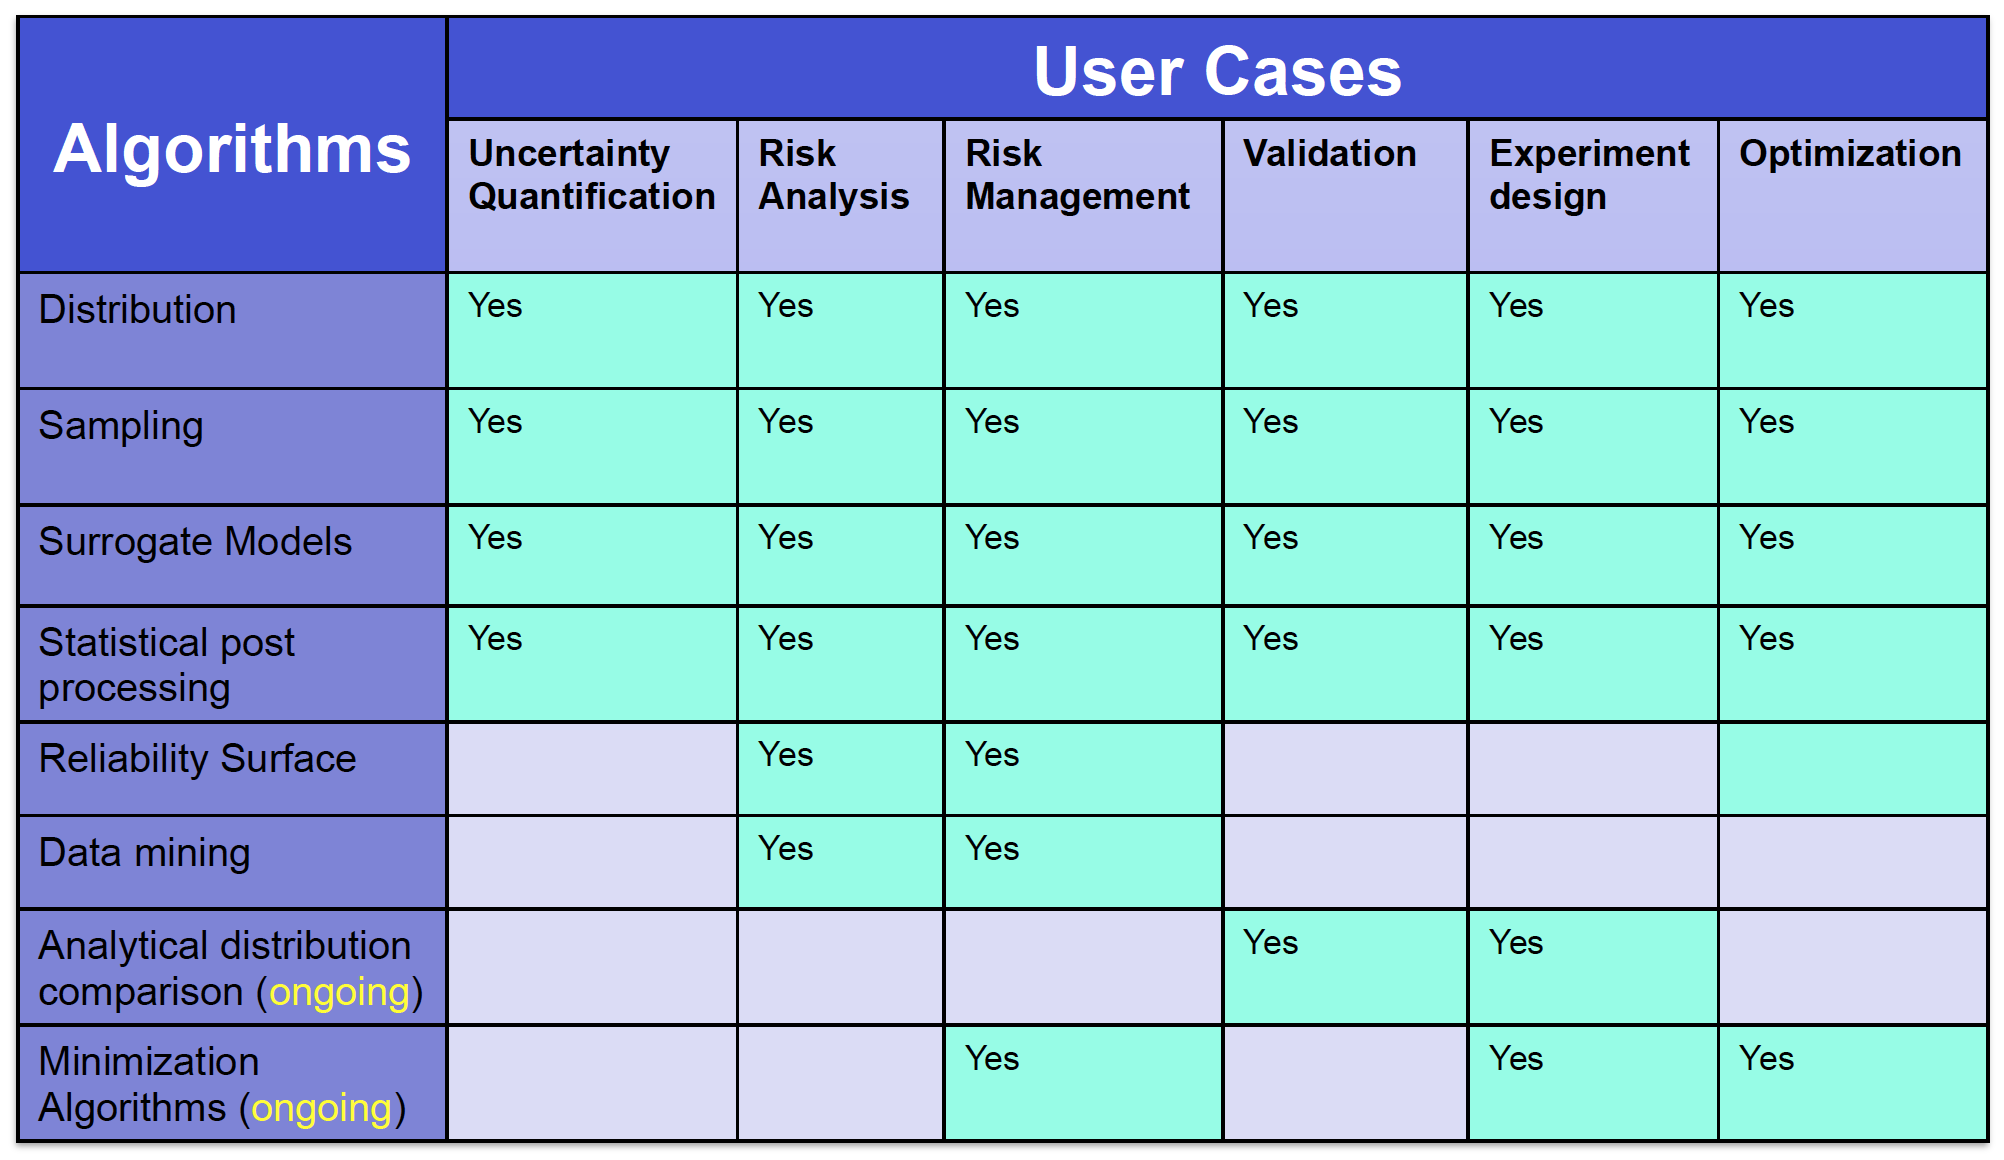
\includegraphics[width=\textwidth]{pics/raven_cap.png}
  \caption{RAVEN Capabilities vs. Needs}
  \label{fig:ravenCap}
\end{figure}

\begin{itemize}
  \item \textbf{Sensitivity Analysis and Uncertainty Quantification}: Sensitivity analysis is a mathematical tool
    that can be used to identify the key sources of uncertainties. Uncertainty quantification is a process by which
    probabilistic information about system responses can be computed according to specified input parameter probability
    distributions. Available approaches in RAVEN include \textbf{Monte Carlo}, \textbf{Grid}, \textbf{Stratified (Latin hypercube)},
    \textbf{Sparse Grid Collocation}, \textbf{Sobol}, \textbf{Adaptive Sparse Grid}, \textbf{Adaptive Sobol} and
    \textbf{BasicStatistics}.
  \item \textbf{Design of Experiments}: The design of experiments (DOE) is a powerful tool that can be used to explore the
    parameter space at a variety of experimental situations. It can be used to determine the relationship between
    input factors and the desired outputs. Available approaches in RAVEN include \textbf{Factorial Design}
    (i.e. General full factorial, 2-level fractional-factorial and Plackett-Burman) and \textbf{Response Surface Design}
    (i.e. Box-Behnken and Central composite algorithms).
  \item \textbf{Risk Mitigation or Model Optimization}: RAVEN uses the \textbf{Optimizer}, a powerful sampler-like entity that searches
    the input space to find minimum or maximum values of a reponse. Currently available optimizers include
    \textbf{Simultaneous Perturbation Stochastic Approximation (SPSA)}.
  \item \textbf{Risk Analysis}: Available approaches in RAVEN include \textbf{Dynamic Event Tree}, \textbf{Limit Surface Search},
    \textbf{Hybrid Dynamic Event Tree}, \textbf{Adaptive Dynamic Event Tree}, \textbf{Adaptive Hybrid Dynamic Event Tree},
    \textbf{Data Mining}, \textbf{Importance Rank}, \textbf{Safest Point}, and \textbf{Basic Statistics}.
  \item \textbf{Risk Management}: Available approaches in RAVEN include \textbf{Reduced order models},
    approaches used for sensitivity and uncertainty analysis, and \textbf{Dynamic Event Tree} methods.
  \item \textbf{Validation}: Available approaches in RAVEN include \textbf{ROMs}, \textbf{Comparison Statistics} and \textbf{Validation Metrics} 
\end{itemize}

In addition, RAVEN includes a number of related advanced capabilities. \textbf{Surrogate or Reduced order models (ROMs)} are mathematical
model trained to predict a response of interest of a physical system. Typically, ROMs trade speed for accuracy representing
a faster, rough estimate of the underlying systems. They can be used to explore the input parameter space for optimization
or sensitivity and uncertainty studies. \textbf{Ensemble Model} is able to combine \textbf{Codes}, \textbf{External Models}
and \textbf{ROMs}. It is intended to create a chain of models whose execution order is determined by the input/output
relationships among them. If the relationships among the models evolve in a non-linear system, a Picard's iteration scheme is
employed.

\subsection{Components of RAVEN}
\label{sub:InputComponents}
The RAVEN code does not have a fixed calculation flow, since all of its basic
objects can be combined in order to create a user-defined calculation flow.
%
Thus, its input, eXtensible Markup Language (XML) format, is organized in different XML blocks, each with a
different functionality. For more information about XML, please click on the link:
\href{https://www.w3schools.com/xml/default.asp}{\textbf{XML tutorial}}.
%
\\The main input blocks are as follows:
\begin{itemize}
  \item \xmlNode{Simulation}: The root node containing the
  entire input, all of
  the following blocks fit inside the \emph{Simulation} block.
  %
  \item \xmlNode{RunInfo}: Specifies the calculation
  settings (number of parallel simulations, etc.).
  %
  \item \xmlNode{Files}: Specifies the files to be
  used in the calculation.
  %
  \item \xmlNode{Distributions}: Defines distributions
  needed for describing parameters, etc.
  %
  \item \xmlNode{Samplers}: Sets up the strategies used for
  exploring an uncertain domain.
  %
  \item \xmlNode{DataObjects}: Specifies internal data objects
  used by RAVEN.
  %
  \item \xmlNode{Databases}: Lists the HDF5 databases used
  as input/output to a
  RAVEN run.
  %
  \item \xmlNode{OutStreams}: Visualization and
  Printing system block.
  %
  \item \xmlNode{Models}: Specifies codes, ROMs,
  post-processing analysis, etc.
  %
  \item \xmlNode{Functions}: Details interfaces to external
  user-defined functions and modules the user will be building and/or running.
  %
  \item \xmlNode{VariableGroups}: Creates a collection of variables.
  %
  \item \xmlNode{Optimizers}: Performs the driving of a specific goal function over
  the model for value optimization.
  %
  \item \xmlNode{Metrics}: Calculate the distance values among points and histories.
  %
  \item \xmlNode{Steps}: Combines other blocks to detail a
  step in the RAVEN workflow including I/O and computations to be performed.
  %
\end{itemize}

Each of these components are explained in dedicated sections of the user manual ~\cite{RAVENuserManual}, and can
be used as building blocks to construct certain calculation flow, as shown in Figure.~\ref{fig:ravenStructure}.
In this guide, we will only show how to use these components to build the analysis flow, and we recommend the user
to check the user manual ~\cite{RAVENuserManual} for the detailed descriptions.

\begin{figure}[h!]
  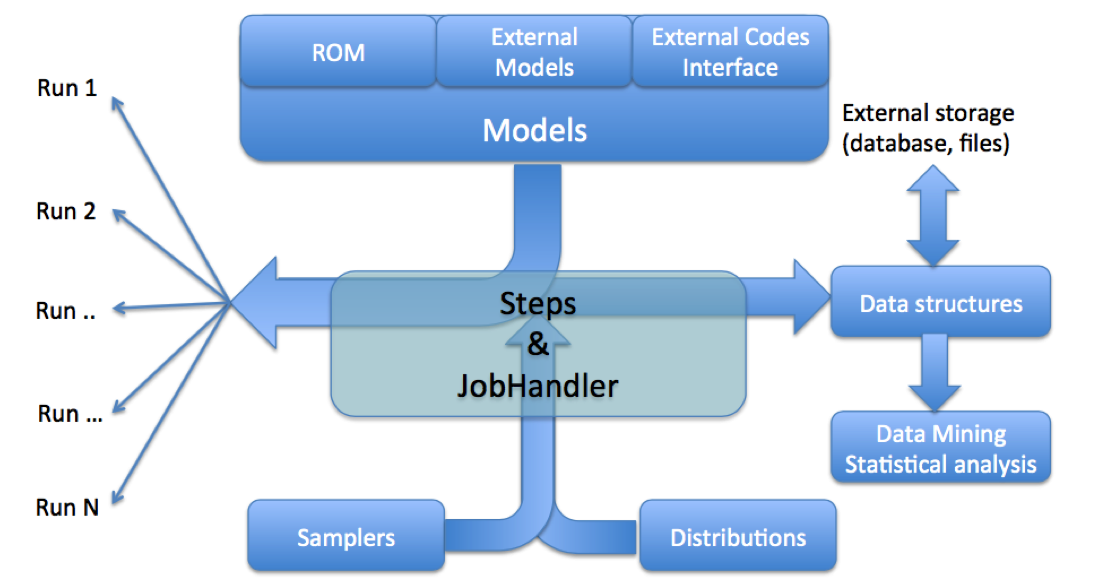
\includegraphics[width=\textwidth]{pics/ravenStructure.png}
  \caption{RAVEN structures}
  \label{fig:ravenStructure}
\end{figure}

In addition, RAVEN allows the user to load any external input file that contains the required XML nodes into the RAVEN main input
file, and provide the standard XML comments, using\verb|<!--| and \verb|-->|. For example, one can use the following template to load
the \xmlNode{Distributions} from file `Distributions.xml'.
%
\begin{lstlisting}[style=XML,morekeywords={node,xmlToLoad}]
<Simulation verbosity='all'>
  ...
  <!-- An Example Comment -->
  <Steps verbosity='debug'>
    ...
  </Steps>
  ...
  <ExternalXML node='Distributions' xmlToLoad='path_to_folder/Distributions.xml'/>
  ...
</Simulation>
\end{lstlisting}
%
RAVEN also allows the user to control the level of output to the user interface by using \xmlAttr{verbosity} system. These settings can be
declared globally as attributes in the \xmlNode{Simulation} node, or locally in each block node as shown in above template.
The verbosity levels are
\begin{itemize}
\item \xmlString{silent} - Only simulation-breaking errors are displayed.
\item \xmlString{quiet} - Errors as well as warnings are displayed.
\item \xmlString{all} (default) - Errors, warnings, and messages are displayed.
\item \xmlString{debug} - For developers. All errors, warnings, messages, and debug messages are displayed.
\end{itemize}



\subsection{Code Interfaces of RAVEN}
The procedure of coupling a new code/application with RAVEN is a straightforward process. The provided Application
Programming Interfaces (APIs) allow RAVEN to interact with any code as long as all the parameters that need to be
perturbed are accessible by input files or via python interfaces. For example, for all the codes currently
supported by RAVEN (e.g. RELAP-7, RELAP-5D, BISON, MAMMOTH, etc.), the coupling is performed through a Python interface
that interprets the information coming from RAVEN and translates them into the input of the driven code. The couping procedure
does not require modifying RAVEN itself. Instread, the developer creates a new Python interface that is going to
be embedded in RAVEN at run-time (no need to introduce hard-coded coupling statements). In addition, RAVEN will
manage concurrent executions of your simulations in parallel, whether on a local desktop or remote high-performance cluster.

Figure.~\ref{fig:modelAPIs} depicts the different APIs between RAVEN and the computational models, i.e. the
\textbf{ROM}, \textbf{External Models} and \textbf{External Code} APIs. 

\begin{figure}[h!]
  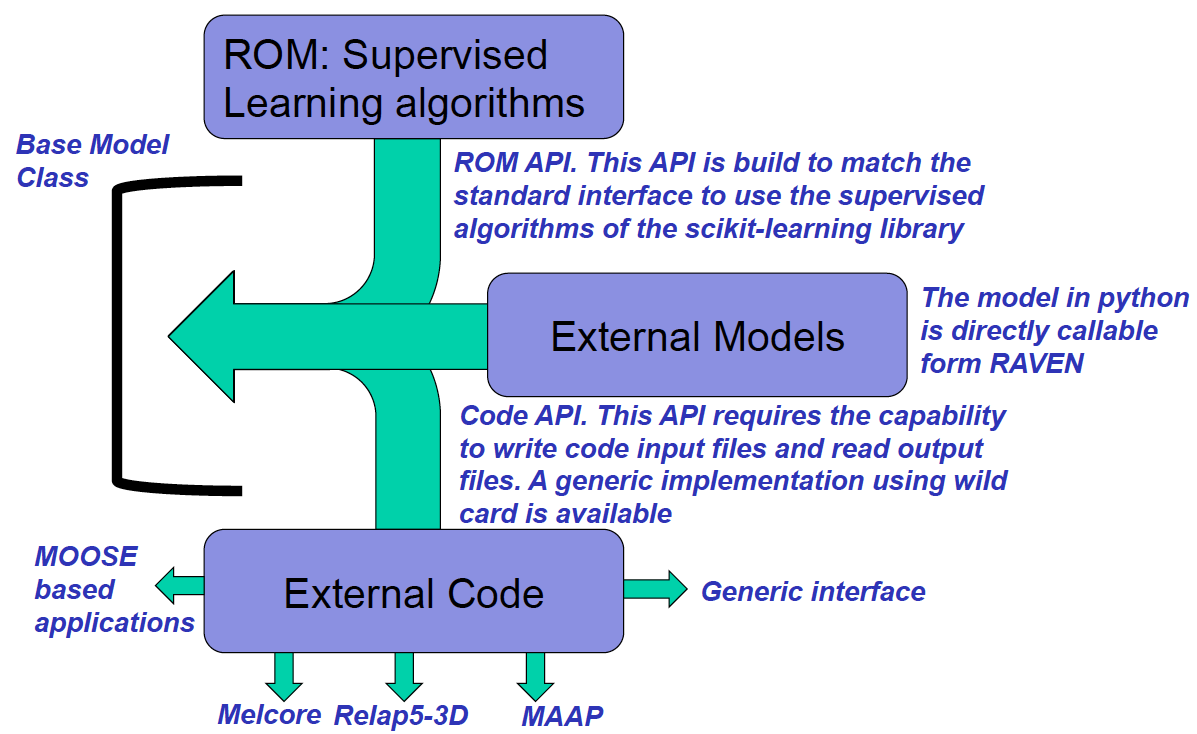
\includegraphics[width=\textwidth]{pics/modelAPIs.png}
  \caption{RAVEN Application Programming Interfaces}
  \label{fig:modelAPIs}
\end{figure}

\clearpage

\subsection{User Guide Organization}
The goal of this document is to provide a set of detailed examples that can help the user to become familiar with
the RAVEN code. RAVEN is capable of investigating system response and explore input space using various
sampling schemes such as Monte Carlo, grid, or Latin Hypercube. However, RAVEN strength lies in its system feature
discovery capabilities such as: constructing limit surfaces, separating regions of the input space leading to
system failure, and using dynamic supervised learning techniques. New users should consult the \textbf{RAVEN Tutorial}
to get started.

\begin{itemize}
  \item \textbf{RAVEN Tutorial}: section~\ref{sec:ravenTutorial}
  \item \textbf{Sampling Strategies}: section~\ref{sec:forwardSamplingStrategies} and section~\ref{sec:adaptiveSamplingStrategies}
  \item \textbf{Restart}: section~\ref{sec:samplingFromRestart}
  \item \textbf{Reduced Order Modeling}: section~\ref{sec:ROMraven}
  \item \textbf{Risk Analysis}: section~\ref{sec:SAraven}
  \item \textbf{Data Mining}: section~\ref{sec:DMraven}
  \item \textbf{Model Optimization}: section~\ref{sec:optimizerStrategies}
  %%%% We may need to add the following sections
  %\item \textbf{Sensitivity Analysis and Uncertainty Quantification}:
  %\item \textbf{Design of Experiments}:
  %\item \textbf{Validation}:
  %\item \textbf{Code Interface}:
  %\item \textbf{Advanced Topics}:
  %  \begin{itemize}
  %    \item Ensemble Forward Sampler:
  %    \item Ensemble Model:
  %  \end{itemize}
\end{itemize}




\section{Manual Formats}
In order to highlight some parts of the Manual having a particular meaning (e.g., input structure, examples, terminal commands, etc.), specific formats have been used. In this sections all the formats with a specific meaning are reported:
\begin{itemize}
\item \textbf{\textit{Python Coding:}}
\begin{lstlisting}[language=python]
class AClass():
  def aMethodImplementation(self):
    pass
\end{lstlisting}
\item \textbf{\textit{XML input example:}}
\begin{lstlisting}[style=XML,morekeywords={anAttribute}]
<MainXMLBlock>
  ...
  <anXMLnode name='anObjectName' anAttribute='aValue'>
     <aSubNode>body</aSubNode>
  </anXMLnode>
  ...
</MainXMLBlock>
\end{lstlisting}
\item \textbf{\textit{Bash Commands:}}
\begin{lstlisting}[language=bash]
cd trunk/raven/
./raven_libs_script.sh
cd ../../
\end{lstlisting}
\end{itemize}


% definitions

% content
\section{Installation}
\subsection{Overview}
\label{sec:install overview}

The installation of the RAVEN code is a straightforward procedure;
depending on the usage purpose and machine architecture, the
installation process slightly differs.

In the following sections, the recommended installation procedure is outlined.  For alternatives, we encourage
checking the \wiki.  The machines on which
RAVEN is tested and developed, however, use the standard installation procedures outlined below.

The installation process will involve three steps:
\begin{itemize}
  \item Installing prerequisites, which depends on your operating system;
  \item Installing conda;
  \item Installing RAVEN.
\end{itemize}

Depending on your operating system (Windows in section \ref{sec:install windows}, MacOSX in section
\ref{sec:install mac}, Ubuntu Linux in section \ref{sec:install ubunutu}), follow the instructions for installing prerequisites, then continue with
installing conda (section \ref{sec:install conda}), and then installing RAVEN (section \ref{sec:clone raven}).


\subsection{Linux Ubuntu Installation}
\label{sec:install ubunutu}
The following instructions are for installing RAVEN on a Linux machine running Ubuntu 16.04 or greater.  Some
explanations of alternatives for other Linux distributions may be provided on the \wiki.

To install the prerequisite packages, the following terminal command should be executed (note this requires
administrative privileges):

\begin{lstlisting}[language=bash]
 sudo apt-get install libtool git python3-dev swig g++
\end{lstlisting}

\paragraph{Optional LateX installation}
Optionally, if you want to be able to edit and rebuild the manuals, you can
install \TeX~Live and its related packages:
\begin{lstlisting}[language=bash]
  sudo apt-get install texlive-latex-base \
  texlive-extra-utils texlive-latex-extra texlive-math-extra
\end{lstlisting}

Once the above are installed, proceed with installing conda (see section \ref{sec:install conda}).

\subsection{Mac OSX Installation}
\label{sec:install mac}

When using an Apple Macintosh computer, software dependencies are met
by following steps:
\begin{itemize}
  \item Install the XCode command line tools from Apple,
  \item Install the XQuartz  X-Window system server,
\end{itemize}

\subsubsection{Installing XCode Command Line Tools}

The XCode command line tools package from Apple Computer provides the C++
compilers and git source code control tools needed to obtain and build RAVEN.
It is freely available from the Apple store. In order to obtain it the following command should be launched in an open terminal:
\begin{lstlisting}[language=bash]
 xcode-select --install
\end{lstlisting}

\subsubsection{Installing XQuartz}
XQuartz is an implementation of the X Server for the Mac OSX operating system.
XQuartz is freely available on the web and can be downloaded from the link
 \url{https://dl.bintray.com/xquartz/downloads/XQuartz-2.7.9.dmg}.
\\After downloaded, install the package.

With XCode and XQuartz installed, continue on to install conda (see section \ref{sec:install conda}).

\nb While \texttt{gcc} and
\texttt{git} are also required, they are installed by default in the OSX system.

\subsection{Microsoft Windows}
\label{sec:install windows}

The process of establishing the required environment for Windows is notably more involved than the other two
systems; however, it is straightforward.  First, RAVEN has the following prerequisites on Windows:

\begin{itemize}
    \item A system running a 64-bit version of Microsoft Windows. Installation and operation
        has been verified on Windows 7, 10, and Windows Server 2012 R2 Standard.
    \item At least 9 Gigabytes of available disk space:
    \begin{itemize}
        \item 0.5 GB for GIT SCM, including supporting tools and git source code control
        \item 1.5 GB for Python language and supporting packages
        \item 1 GB for RAVEN framework
        \item 5.0 GB for the Visual Studio compiler needed to build RAVEN
    \end{itemize}
\end{itemize}

\subsubsection{A Visual Guide}
Note: An illustrated version of this procedure may be found on the \wiki.

\subsubsection{GIT SCM for Windows}
RAVEN currently works on Windows using basic tools freely available online. 
The first software to be downloaded and installed is \textbf{Git SCM} available at \url{https://gitforwindows.org/}.
\begin{enumerate}
    \item Obtain the latest Git SCM for Windows installer from  \url{https://gitforwindows.org/} and install it. 
    Install Git Bash and have 
    the installer add Git Bash to your Windows \textit{PATH} environment variables. 
    The \textit{PATH} can be updated either automatically (allowing the Git SCM installer to update it for you) or manually 
    (Systems Properties - Environment Variables - Edit Environment Variables).
\end{enumerate}

\subsubsection{Install Python Language and Package Support}
\begin{enumerate} 
	\item Download the latest 64-bit installer for Windows Python 3 from
		\url{https://conda.io/miniconda.html} and install it.  \item The installer
		will ask whether Python should be installed for only the logged in user or
		for all users.  Either option will work for RAVEN.
	\item 	have  the installer add \textit{conda} to your Windows \textit{PATH} environment variables.   
	The \textit{PATH} can be updated either automatically (allowing the  \textit{conda} installer to update it for you) 
	or manually (Systems Properties - Environment Variables - Edit Environment Variables).
	\item Check the installation of Python and coda locating and testing the Python installation.   
	Open a Windows command prompt and enter the
		command "{\it where python}", which attempts to locate a the Python language interpreter
		in the current system path.  This looks like:

    \begin{lstlisting}[language=bash, basicstyle=\small]
    C:\Users\USERID> where python
    C:\Users\USERID\AppData\Local\Continuum\Miniconda3\python.exe
    \end{lstlisting}

\end{enumerate}


\subsubsection{Compiler Installation and Configuration}
\begin{enumerate}
	\item Download and install Visual Studio.  A C++ language compiler that supports C++11 features
		is needed to perform this step. Microsoft's Visual Studio Community Edition is free and
		available from \url{https://www.visualstudio.com/downloads/}.

		The current version (as of this writing) is 2017. The 2015 and 2017 versions have been
		successfully used to build RAVEN. Professional and Enterprise versions of these will
		also work. If one of these is already present on your system, it is not necessary to
		obtain another one. Note that because C++11 language features are required, the
		"Microsoft Visual C++ Compiler for Python 2.7 or 3.x" often used for building Python
		add-ons will {\bf not} work.

		After downloading and running the Visual Studio installer, it will ask what features
		to install. For building RAVEN, "Desktop development with C++" is needed at a minimum.
		Installation of other Visual Studio features should be fine.
\end{enumerate}

Once the compiler installation and configuration is complete, you are prepared to install the RAVEN libraries
(see section \ref{sec:install conda}).




\subsection{Conda: Python Dependencies}
\label{sec:install conda}

The standard installation procedure for RAVEN includes using Miniconda (often simply referred to as
\emph{conda}) to install the Python libraries required to run RAVEN.  If conda cannot be made available on an
operating system, refer to the wiki (listed above) for alternatives.  To install miniconda, follow the
instructions for your operating system at \url{https://conda.io/miniconda.html}.

\nb RAVEN currently works with Python 2.7, but it is recommended that Python 3 be used, so unless you have a reason to use 2.7, we recommend installing the 64 bit Python 3 version of miniconda.

Once conda is installed, proceed to installing RAVEN itself (section \ref{sec:clone raven}).


\subsection{Installing RAVEN}
\label{sec:clone raven}

Once the RAVEN dependencies have been installed  and conda is present
(see section \ref{sec:install overview}), the rest of RAVEN can be installed.

The installation of RAVEN involves the following steps:
\begin{itemize}
  \item Obtain the source code,
  \item Install the prerequisite Python libraries using conda,
  \item Compile
\end{itemize}




\subsubsection{Obtaining RAVEN Source Code}
RAVEN is hosted publicly as a \texttt{Git} repo on \texttt{GitHub}
and can be viewed at \url{https://github.com/idaholab/raven/wiki}.
In the event that access to \texttt{GitHub} is impossible, contact the user list and other arrangements may be
possible.  In general, however, using the git repository assures the most consistent usage and update process.

To clone RAVEN, navigate in a terminal to the desired destination, for example \texttt{~/projects}.  Then run
the commands
\begin{lstlisting}[language=bash]
git clone https://github.com/idaholab/raven.git
cd raven
git submodule update --init
\end{lstlisting}
This will obtain RAVEN as well as other submodules that RAVEN uses.  In the future, whenever we declare a path
starting with \texttt{raven/}, we refer to the cloned directory.




\subsubsection{Installing Python Libraries}
RAVEN depends heavily on Python, and uses conda to maintain a separate environment to prevent conflicts with
other Python library installations.  This separate environment is called \texttt{raven\_libraries}.

In order to establish this environment, navigate to \texttt{raven}, then
\begin{itemize}

  \item \textbf{Any unix-based systems (e.g. Macintosh, Linux, etc.)}:
\begin{lstlisting}[language=bash]
cd scripts
./establish_conda_env.sh --install
\end{lstlisting}
  \item \textbf{Windows}:
  \begin{lstlisting}[language=bash]
cd scripts
bash.exe establish_conda_env.sh --install
\end{lstlisting}
  
\end{itemize}
Assure that there are no errors in this process, then continue to compiling RAVEN.

\nb If \texttt{conda} is not installed in the default location, then the path to the conda definitions
needs to be provided, for example

\begin{itemize}

  \item \textbf{Any unix-based systems (e.g. Macintosh, Linux, etc.)}:
\begin{lstlisting}[language=bash]
cd scripts
./establish_conda_env.sh --install
   --conda-defs /path/to/miniconda3/etc/profile.d/conda.sh
\end{lstlisting}
  \item \textbf{Windows}:
  \begin{lstlisting}[language=bash]
cd scripts
bash.exe establish_conda_env.sh --install
  --conda-defs \path/\to\miniconda3\etc\profile.d\conda.sh
\end{lstlisting}
  
\end{itemize}

replacing \texttt{/path/to} with the install path for \texttt{conda}.

\nb Various options exist for \texttt{establish\_conda\_env.sh}, which
can be found by using the \texttt{--help} option.  These options
include \texttt{--mamba} which uses the mamba instead of conda for
resolving dependencies, \texttt{--load} which can be used with
\verb'source ./scripts/establish_conda_env.sh --load' to switch to the
raven environment in a shell, \texttt{--installation-manager PIP} which
uses pip instead of conda.

\subsubsection{Compiling RAVEN}
Once Python libraries are established and the source code present, navigate to \texttt{raven} and run


\begin{itemize}

  \item \textbf{Any unix-based systems (e.g. Macintosh, Linux, etc.)}:
\begin{lstlisting}[language=bash]
./build_raven
\end{lstlisting}
  \item \textbf{Windows}:
  \begin{lstlisting}[language=bash]
bash.exe build_raven
\end{lstlisting}
  
\end{itemize}

This will compile several dependent libraries.  This step has the highest potential for revealing problems in
the operating system setup, particularly for Windows.  See troubleshooting on the \wiki for help sorting out
difficulties.


\subsubsection{Testing RAVEN}
\label{sec:testing raven}
To test the installation of RAVEN, navigate to \texttt{raven}, then run the command

\begin{itemize}

  \item \textbf{Any unix-based systems (e.g. Macintosh, Linux, etc.)}:
\begin{lstlisting}[language=bash]
../run_tests -j2
\end{lstlisting}
  \item \textbf{Windows}:
  \begin{lstlisting}[language=bash]
bash.exe ./run_tests -j2
\end{lstlisting}
  
\end{itemize}

where \texttt{-j2} signifies running with 2 processors.  If more processors are available, this can be
increased, but using all or more than all of the available processes can slow down the testing dramatically.
This command runs RAVEN's regression tests, analytic tests, and unit tests.  The number of tests changes
frequently as the code's needs change, and the time taken to run the tests depends strongly on the number of
processors and processor speed.

At the end of the tests, a number passed, skipped, and failing will be reported.  Having some skipped tests is
expected; RAVEN has many tests that apply only to particular configurations or codes that are not present on
all machines.  However, no tests should fail; if there are problems, consult the troubleshooting section on
the \wiki.


\subsubsection{Updating RAVEN}
RAVEN updates frequently, and new features are added while bugs are fixed on a regular basis.  To update
RAVEN, navigate to \texttt{raven}, then run the commands
\begin{itemize}

  \item \textbf{Any unix-based systems (e.g. Macintosh, Linux, etc.)}:
\begin{lstlisting}[language=bash]
git pull
./scripts/establish_conda_env.sh --install
./build_raven
\end{lstlisting}
  \item \textbf{Windows}:
  \begin{lstlisting}[language=bash]
git pull
bash.exe scripts/establish_conda_env.sh --install
bash.exe build_raven
\end{lstlisting}
  
\end{itemize}

\subsubsection{In-use Testing}
Whenever RAVEN is installed on a new computer or whenever there is a significant change to the operating system, 
in-use tests shall be conducted.
Acceptable performance of RAVEN shall be confirmed by running the installation tests as described in  \ref{sec:testing raven}.


\section{Running RAVEN}
\label{HowToRun}

% I don't think this is mentioned earlier? Andrea answers :D It mentioned in the Introduction
%As already mentioned,
The RAVEN code is a blend of C++, C, and Python software. The entry point
resides on the Python side and is accessible via a command line interface.
%
After following the instructions in the previous Section, RAVEN is ready to be
used.
%
The \texttt{raven\_framework} script is in the raven folder.
%
To run RAVEN, open a terminal and use the following command (replace \texttt{<inputFileName.xml>} with your RAVEN input file):

\begin{itemize}

  \item \textbf{Any unix-based systems (e.g. Macintosh, Linux, etc.)}:
\begin{lstlisting}[language=bash]
raven_framework <inputFileName.xml>
\end{lstlisting}
  \item \textbf{Windows}:
  \begin{lstlisting}[language=bash]
bash.exe raven_framework <inputFileName.xml>
\end{lstlisting}
  
\end{itemize}

Using \texttt{raven\_framework} is the recommended way to run RAVEN.  In the event bypassing the typical
environment loading and checks is desired, it can also be run via
the \texttt{raven\_framework.py} script using python, with the input file as argument.  However, this is not
recommended, as it will use whatever default versions of Python and other libraries are discovered, rather
than the matching libraries set up during installation.

\nb For Windows systems, we provided a convenient Batch script ( \texttt{raven\_framework.bat} ) for running RAVEN 
avoiding to interact with the Windows command line terminal. More info on how to use it can be found in the RAVEN
\wiki , section \textit{Running RAVEN} (\url{https://github.com/idaholab/raven/wiki/runningRAVEN}).


\section{RAVEN Mathematical Background}
\label{sec:mathBackground}
\subsection{System and Control Model}
\label{sub:controlAndSystem}
The first step is the derivation of the mathematical model representing, with a high
level of abstraction, the plant and control system model. Let $\overline{\theta}\left ( t
\right )$ be a vector describing the system status in the phase space, characterized
by the following governing equation:
\begin{equation}
\label{eq:dThetaOverDT}
\frac{\partial \overline{\theta} }{\partial t}=\overline{H}\left (  \overline{\theta}\left ( t \right ),t \right )
\end{equation}
In Equation above, the assumption of time differentiability of the trajectory equation $\overline{H}\left (  \overline{\theta}\left ( t \right ),t \right )$ in the phase space has been taken. This assumption is not fully correct and generally required and it is used here, without missing of generality, for compactness of the notation.
\\It can now be performed an arbitrary decomposition of the phase space:
\begin{equation}
\label{eq:thetaDecomposition}
  \overline{\theta} = \left (\frac{\overline{x}}{\overline{v}}  \right )
\end{equation}
The decomposition is made in such a way that $\overline{x}$ represent the unknowns
solved by a system code (such as RELAP5-3D~\cite{RELAP5userManual},
RELAP7~\cite{relap7FY12}, etc.) while $\overline{v}$ are the variables directly
controlled by the control system (e.g., automatic mitigation systems, operator actions,
etc.).
\\The governing equation can be now cast in the following system of equations:
\begin{equation}
\label{eq:governingEquations}
\left\{\begin{matrix}
\frac{\partial \overline{x} }{\partial t} = \overline{F}\left (  \overline{x}, \overline{v}, t \right )  \\
\frac{\partial \overline{v} }{\partial t} = \overline{V}\left (  \overline{x}, \overline{v}, t \right )
\end{matrix}\right.
\end{equation}
Consequentially to this splitting, $\overline{x}$ contains the state variables of the
phase space that are continuous while $\overline{v}$ contains discrete state
variables that are usually handled by the control system (consequentially, named
\textbf{control variables}). It can be noticed that the
function  $ \overline{V}\left (  \overline{x}, \overline{v}, t \right )$, representing the
control system, does not depend on the  knowledge of the complete status of the
system but on a restricted subset that can be named \textbf{monitored variables} $\overline{C}$:

\begin{equation}
\label{eq:controlVars}
\left\{\begin{matrix}
\frac{\partial \overline{x} }{\partial t} = \overline{F}\left (  \overline{x}, \overline{v}, t \right )  \\
 \overline{C} =  \overline{G}(\overline{x},t)     \\
\frac{\partial \overline{v} }{\partial t} = \overline{V}\left (  \overline{x}, \overline{v}, t \right )
\end{matrix}\right.
\end{equation}
where $\overline{C}$ is a vector of smaller dimensionality than $\overline{x}$ and,
therefore, more convenient to handle.
\\As it can be noticed, the standard nomenclature of \textit{signals} (monitored variables) and \textit{status} (control variables) is not adopted. Two principal reasons
justify this decision:
\begin{itemize}
  \item The definition of signals is tight to the definition of the
  control logic for each component and, therefore, relative rather than absolute in the
  overall system analysis. For example, it is possible the the \textit{signals} for a
  component represent \textit{status} of another one, determining an in-unique
  definition.
  \item The standard nomenclature becomes meaningless when this derivation is
  applied to Uncertainty Quantification (UQ).
\end{itemize}

\subsubsection{Splitting Approach for the Simulation of the Control System}
Equation~\ref{eq:controlVars} represents a fully coupled system of Partial Differential
Equations (PDEs). To solve this system, an  \textit{operator splitting} approach
is employed. This method is preferable in this context for several reasons, among which the following:
\begin{itemize}
  \item In reality, the control system (automatic mitigation systems, operator actions,
  etc.) is always characterized by an intrinsic delay
  \item The reaction of the control system might make the system ``move'' among
  different discrete states; therefore, numerical errors will be always of first order
  unless the discontinuity is explicitly treated.
\end{itemize}
Employing the \textit{operator splitting} approach, Equation ~\ref{eq:controlVars}  can be
cast as follows:
\begin{equation}
\label{eq:operatorSplitting}
\left\{\begin{matrix}
\frac{\partial \overline{x} }{\partial t} = \overline{F}\left (  \overline{x},\overline{v}_{t_{i-1}}, t \right )  & \\
\overline{C} =  \overline{G}(\overline{x},t)  & t_{i-1} \leq t \leq  t_{i} =  t_{i-1} + \Delta  t_{i}\\
\frac{\partial \overline{v} }{\partial t} = \overline{V}\left (  \overline{x}, \overline{v}_{t_{i-1}}, t \right ) &
\end{matrix}\right.
\end{equation}
Hence, the system of equations in solved decomposing it into simpler sub-problems that are treated individually
using specialized numerical algorithms.

\subsubsection{Definition of the Monitored Variable Space}
The contraction of the information from the $\overline{x}$ space to the $\overline{C}$ space is a crucial step.
Since $\overline{C}$ represents an arbitrary middle step, it is needed to define a set of rules that make this
choice unique. $\overline{C}$ is chosen such that:
\begin{itemize}
  \item The solution of  $ \left.\begin{matrix} \frac{\partial \overline{v} }{\partial t}
  \end{matrix}\right| =\overline{V}\left (  \overline{x},\overline{v}_{t_{i-1}}, t \right )$
  can be carried along without any knowledge of the solution algorithm of
   $ \left.\begin{matrix}
  \frac{\partial \overline{x} }{\partial t} =  \end{matrix}\right| \overline{F}\left (
  \overline{x},\overline{v}_{t_{i-1}}, t \right )
  $. This requirement determines the minimum information contraction from  $\overline{x}$ to
  $\overline{C}$.
  \item All actions represented by $\overline{C} = \overline{G}(\overline{x},t)$ require knowledge of the
  solution algorithm of
  $ \left.\begin{matrix}
  \frac{\partial \overline{x} }{\partial t} =  \end{matrix}\right| \overline{F}\left (
  \overline{x},\overline{v}_{t_{i-1}}, t \right )  $. This requirement determines  the maximum  information contraction from  $\overline{x}$ to  $\overline{C}$.
\end{itemize}
The intersection of the two sub-spaces defined above create a minimal unique set.
\subsubsection{Definition of the Auxiliary Variable Space}
In the previous sections, it has been determined that the needed information to model the dynamic system
is contained in the solution vectors $\overline{x}$ and $\overline{v}$. Even if $\overline{x}$ and $\overline{v}$
are sufficient to assess the system status at every point in time, it can result in an unpractical way to model
the eventual control system.
Let's suppose to model a component of a particular system that presents different behavior depending on
other systems or operation behaviors. In order to define the status of this component in every point in time, the
whole history of the system needs to be tracked. In order to remove these inefficiency, a set of auxiliary variables
$\overline{a}$ can be introduced. These variables are the ones that in the analysis of stochastic dynamics
are artificially added into the phase space to a non-Markovian system to obtain back a Markovian behavior. In this
way only the previous time-step information is needed to determine the status of the system.
\\ Adding this additional system of variables, Equation ~\ref{eq:operatorSplitting} can be casted as follows:

\begin{equation}
\label{eq:auxiliaryVariables}
\left\{\begin{matrix}
\frac{\partial \overline{x} }{\partial t} = \overline{F}\left (  \overline{x},\overline{v}_{t_{i-1}}, t \right )  & \\
\overline{C} =  \overline{G}(\overline{x},t)  & t_{i-1} \leq t \leq  t_{i} =  t_{i-1} + \Delta  t_{i}\: \\
\frac{\partial \overline{a} }{\partial t} = \overline{A}\left (  \overline{x},\overline{C},\overline{a},\overline{v}_{t_{i-1}}, t \right ) \\
\frac{\partial \overline{v} }{\partial t} = \overline{V}\left (  \overline{C},\overline{a}, \overline{v}_{t_{i-1}}, t \right )  &
\end{matrix}\right.
\end{equation}

\subsection{Dynamic Systems Stochastic Modeling}
%
\subsubsection{General system of equations and variable classification}
\label{subsub:generalSystemOfEqAndVarsClassification}
In Section ~\ref{sub:controlAndSystem}, the derivation of the governing equations for a controllable system
have been reported. In this section, the mathematical framework of the modeling of dynamic stochastic systems,
under uncertainties, is derived.
\\ Dynamic stochastic systems are the ones whose dynamic is characterized by intrinsic randomness. Random
behaviors, although present in nature, are often artificially introduced into physical models to account for the
incapability of fully modeling part of the nature of the system behavior and/or of the phenomena bounding the
physical problem.
\\The distinction between variables that are artificially considered aleatory and the ones intrinsically aleatory
corresponds with the classical definition of epistemic and aleatory uncertainties. From a
system simulation point of view it is more relevant how these variables, the sources of aleatory behavior, change
in time.
Possible examples of random elements are:
\begin{itemize}
 \item random variability of parameters (e.g., uncertainty in physical parameters)
 \item presence of noise (background noise due to intrinsically stochastic behaviors or lack of detail in the
 simulation)
 \item Uncertainty in the initial and boundary conditions
 \item Random failure of components
 \item aging effects.
\end{itemize}
Before introducing the mathematical models for uncertainty,  it can beneficial to recall
Equation ~\ref{eq:dThetaOverDT}, adding the initial conditions:
\begin{equation}
\label{eq:dThetaOverDTWithBoundary}
\left\{\begin{matrix}
\frac{\partial  \overline{\theta}\left ( t \right )}{\partial t}=\overline{H}\left (  \overline{\theta}\left ( t \right ),t \right ) \\
 \overline{\theta}\left ( t_{0} \right ) = \overline{\theta}_{0}
\end{matrix}\right.
\end{equation}
At this point, each source of uncertainty or stochastic behavior is considered and progressively added in
Equation ~\ref{eq:dThetaOverDTWithBoundary}.
For the scope of this derivation, it is convenient to split the phase space into \textit{continuous} (e.g.,temperature,
pressure, hentalpy, etc.) and discrete (e.g.,status of components, such as operational and failure states) variables
as follows:
\begin{itemize}
 \item $ \overline{\theta}^{c} \in \Phi \subseteq \mathbb{R}^{C}$, the set of continuous variables
 \item $ \overline{\theta}^{d} \in \Psi \subseteq \mathbb{N}^{D}$, the set of discrete variables
 \item $\overline{\theta}(t) = \overline{\theta}^{c} \oplus \overline{\theta}^{d}$.
\end{itemize}
Consequentially, Equation ~\ref{eq:dThetaOverDTWithBoundary} assumes the following form:
\begin{equation}
\label{eq:systemThetaContAndDescrete}
\left\{\begin{matrix}
\frac{\partial  \overline{\theta}^{c}\left ( t \right )}{\partial t}=f\left ( \overline{\theta}^{c},\overline{\theta}^{d},t \right ) \\
\frac{\partial  \overline{\theta}^{d}\left ( t \right )}{\partial t}=g\left ( \overline{\theta}^{c},\overline{\theta}^{d},t \right )\\
 \overline{\theta}^{c}\left ( t_{0} \right ) = \overline{\theta}^{c}_{0}\\
 \overline{\theta}^{d}\left ( t_{0} \right ) = \overline{\theta}^{d}_{0}
\end{matrix}\right.
\end{equation}
Note that the time derivative operator has been also used for the time discontinuous variables, even
if this is allowed only introducing complex extension of the time derivative operator. In this context, the $\frac{\partial  }{\partial t}$ on the discontinuous space is employed for simplifying the notation only.

\subsubsection{Probabilistic Nature of the Parameters Characterizing the Equation}
As shown in Equation ~\ref{eq:systemThetaContAndDescreteStaz}, The first stochastic behaviors to be introduced are the
uncertainties associated with the:
\begin{itemize}
  \item initial conditions (i.e. $\overline{\theta}^{c}$ and $\overline{\theta}^{d}$ at time $t_{0}$), and
  \item parameters characteristic of  $f\left ( \overline{\theta}^{c},\overline{\theta}^{d},t \right )$ and $g\left ( \overline{\theta}^{c},\overline{\theta}^{d},t \right )$.
\end{itemize}

\begin{equation}
\label{eq:systemThetaContAndDescreteStaz}
\left\{\begin{matrix}
\frac{\partial  \overline{\theta}^{c}\left ( t \right )}{\partial t}=f\left ( \overline{\theta}^{c},\overline{\theta}^{d}, \overline{\alpha}_{staz} ,      t \right ) \\
\frac{\partial  \overline{\theta}^{d}\left ( t \right )}{\partial t}=g\left ( \overline{\theta}^{c},\overline{\theta}^{d},\overline{\alpha}_{staz},t \right )\\
\Pi \left ( \overline{\theta}^{c},t_{0} \right ) \sim pdf\left ( \overline{\theta}^{c}_{0}|,\sigma_{c}^{2} \right )\\
\Pi \left ( \overline{\theta}^{d},t_{0} \right ) \sim pdf\left ( \overline{\theta}^{d}_{0}|,\sigma_{d}^{2} \right ) \\
\overline{\alpha}_{staz}\left ( t \right )=\overline{\alpha}_{staz}\left ( t_{0} \right ) \sim pdf\left ( \overline{\alpha}_{staz}^{0}|, \sigma_{staz}^{2} \right )
\end{matrix}\right.
\end{equation}
In Equation ~\ref{eq:systemThetaContAndDescreteStaz}, $\Pi \left ( \overline{\theta}^{c},t_{0} \right )$ indicates the
probability distribution of $\overline{\theta}^{c}$ at the initial time $t=t_{0}$ while
$pdf\left ( \mu|, \sigma^{2} \right )$ represents a generic probability distribution function having mean value
$\mu$ and sigma $\sigma$.The term $\overline{\alpha}_{staz}$ is the vector of parameters affected by
uncertainty but not varying over time.
\\As already mentioned, Equation ~\ref{eq:systemThetaContAndDescreteStaz} considers uncertainties whose values
do not change during the dynamic evolution of the system. This set of uncertainties accounts for most of the
common source of aleatory behaviors. Examples of this kind of uncertainties are:
\begin{itemize}
  \item \textit{Uncertainty associated with the heat conduction coefficient}:  This value is known (but uncertain) and has no physical reason to change during the simulation;
  \item \textit{Uncertainty on failure temperature for a pipe}: This value is usually characterized by a probability distribution function but once the value has been set (like through random sampling) it will not change during the simulation.
\end{itemize}
From a modeling perspective, all the probabilistic behaviors connected to $\Pi \left ( \overline{\theta}^{c},t_{0}
\right ) $, $\Pi \left ( \overline{\theta}^{d},t_{0} \right )$ and $\overline{\alpha}_{staz}(t)$ can be modeled without
changing the dimensionality of the phase space (hence, no alteration of the solution algorithm is required), simply performing sampling of the input space. In addition, the Markovian assumption is still preserved.

\subsubsection{Variables Subject to Random Motion}
The next aleatory component to be accounted for is the set of parameters that continuously change over time (i.e. $\overline{\alpha}_{brow}$).
In other words,  these parameters are referred as if they behave like a \textit{Brownian motion}.
While what commonly is indicated as \textit{Brownian motion} has not impact at the character
the space and time scales (characteristic of a physical system), there are parameters that have (or \textbf{appear}
to have) such behavior. The  \textit{Brownian motion} characteristic of some variables can be completely
synthetic, due to the lack of modeling details in the simulation model.
\\For instance, two examples of these randomly varying variables are:
\begin{itemize}
  \item \textit{Cumulative damage growth in material}. Experimental data and models representing this
  phenomenon show large uncertainties. There is also an intrinsic natural stochasticity driving
  the accumulation of the damage (natural Brownian motion);
  \item \textit{Heat conductivity in the fuel gap during heating of fuel}. During some transients there are
  situations where the fuel is in contact with the clad while in others where there is the presence of a gap. While in
  nature this is a discontinuous transition, it is not usually possible to model in such a way, especially if vibrations
  of the fuel lead to high frequency oscillations. In this case, it would be helpful to introduce directly into the
  simulation a random noise characterizing the thermal conductivity when these transitions occur (synthetic
  Brownian motion).
\end{itemize}
The system of Equations~\ref{eq:systemThetaContAndDescreteStaz} can be rewritten in the following form:

\begin{equation}
\label{eq:systemThetaContAndDescreteStazAndBrow}
\left\{\begin{matrix}
\frac{\partial  \overline{\theta}^{c}\left ( t \right )}{\partial t}=f\left ( \overline{\theta}^{c},\overline{\theta}^{d}, \overline{\alpha}_{staz} ,\overline{\alpha}_{brow},      t \right ) \\
\frac{\partial  \overline{\theta}^{d}\left ( t \right )}{\partial t}=g\left ( \overline{\theta}^{c},\overline{\theta}^{d},\overline{\alpha}_{staz},\overline{\alpha}_{brow},t \right )\\
\frac{\partial \overline{\alpha}_{brow} }{\partial t}=b\left ( \overline{\theta}^{c},\overline{\theta}^{d},\overline{\alpha}_{staz},\overline{\alpha}_{brow},t \right )\Gamma \left ( t \right )
\\
\Pi \left ( \overline{\theta}^{c},t_{0} \right ) \sim pdf\left ( \overline{\theta}^{c}_{0}|,\sigma_{c}^{2} \right )\\
\Pi \left ( \overline{\theta}^{d},t_{0} \right ) \sim pdf\left ( \overline{\theta}^{d}_{0}|,\sigma_{d}^{2} \right ) \\
\overline{\alpha}_{staz}\left ( t \right )=\overline{\alpha}_{staz}\left ( t_{0} \right ) \sim pdf\left ( \overline{\alpha}_{staz}^{0}|, \sigma_{staz}^{2} \right ) \\
\overline{\alpha}_{brow}\left ( t_{0} \right ) \sim  \overline{\alpha}_{brow}^{0} \Gamma \left ( t_{0} \right )
\end{matrix}\right.
\end{equation}
where $\Gamma \left ( t \right )$ is 0-mean random noise and $\overline{\alpha}_{brow}$ is the set of parameters subject to \textit{Brownian motion}.
\\Clearly, the equation referring to the time change of the parameters subject to the \textit{Brownian motion} should be interpreted in the \textbf{Ito} sense [C. Gardiner, Stochastic Methods, Springer (2009)].

\subsubsection{Discontinuously and Stochastically varying variables}
The last and probably most difficult step is the introduction of parameters that are neither constant during the simulation nor continuously vary over time. As an example, consider a valve that, provided set of operating conditions, opens or closes. If this set of conditions is reached n times during the simulation, the probability of the valve correctly operating should be sampled n times. It is also foreseeable that the history of failure/success of the valve will impact future probability of failure/success.  In this case the time evolution of such parameters (discontinuously stochastic changing parameters  $\overline{\alpha}_{DS}$) is governed by the following equation:

\begin{equation}
\label{eq:systemDiscAndStochVaryVars}
\frac{\partial  \overline{\alpha }_{DS}\left ( t \right )}{\partial t}=  \overline{\delta}\left ( \overline{\alpha }_{DS}, \overline{\theta}^{c},\overline{\theta}^{d},\overline{\alpha}_{staz},\overline{\alpha}_{brow},t \right ) \times \overline{V}\left ( \overline{\alpha }_{DS}, \overline{\theta}^{c},\overline{\theta}^{d},\overline{\alpha}_{staz},\overline{\alpha}_{brow},t \right ) \times \overline{p}\left ( \int_{t_{0}}^{t}  S\left ( \overline{\theta}\left ( t^{'} \right ),t^{'} \right )dt^{'} \right )
\end{equation}
where:
\begin{itemize}
  \item The function $\overline{\delta}\left ( \overline{\alpha }_{DS}, \overline{\theta}^{c},\overline{\theta}^{d},
  \overline{\alpha}_{staz},\overline{\alpha}_{brow},t \right )$ is the delta of Dirac of the instant on which the
  transition need to be evaluated (control logic signaling to the valve to open/close).
  \item The term $\overline{p}\left ( \int_{t_{0}}^{t}  S\left ( \overline{\theta}\left ( t^{'} \right ),t^{'} \right )\right )
  = \overline{p}\left ( \int_{t_{0}}^{t}  \overline{\alpha }_{DS}, \overline{\theta}^{c},\overline{\theta}^{d},
  \overline{\alpha}_{staz},\overline{\alpha}_{brow},t dt\right )$ represents the transition probability
  between different states (in case of the valve: open/close). Note that the time integral of the
  parameter history accounts for the memory of the component via the kernel $S\left ( \overline{\theta}\left ( t^{'}
  \right ),t^{'} \right )$.
  \item The term $\overline{V}\left ( \overline{\alpha }_{DS}, \overline{\theta}^{c},\overline{\theta}^{d},
  \overline{\alpha}_{staz},\overline{\alpha}_{brow},t \right )$ is the rate of change of $\overline{\alpha }_{DS}$.
  For a discrete parameter, it is defined as the value of the instantaneous $\overline{\alpha }_{DS}$ change.
\end{itemize}
The introduction of the history dependency introduced in the term $\overline{p}$ determines that the system cannot be considered
Markovian if ``countermeasures'' are not taken. In order to make the system return to be Markovian, the phase space needs to be
expanded (i.e., increase its dimensionality): the time at which the
parameters changed status and their corresponding values $\left \{  \left (\overline{\alpha}_{DS}, t \right )_{i} \right \} = \left \{  \overline{\alpha}_{DS}, t_{i} \right \} = \overline{\overline{\alpha}}_{DS}, \overline{t}\, \left ( for\, i=1,...,n \right )$.
\\Equation~\ref{eq:systemDiscAndStochVaryVars} now assumes the form:
\begin{equation}
\label{eq:systemDiscAndStochVaryVarsExpanded}
\begin{matrix}
\frac{\partial  \overline{\alpha }_{DS}\left ( t \right )}{\partial t}=  \overline{\delta}\left ( \overline{\alpha }_{DS}, \overline{\theta}^{c},\overline{\theta}^{d},\overline{\alpha}_{staz},\overline{\alpha}_{brow},t \right ) \times \overline{V}\left ( \overline{\alpha }_{DS}, \overline{\theta}^{c},\overline{\theta}^{d},\overline{\alpha}_{staz},\overline{\alpha}_{brow},t \right ) \times \overline{p}\left ( \overline{\overline{\alpha}}_{DS},\overline{t},\overline{\theta}^{c},\overline{\theta}^{d},\overline{\alpha}_{staz},\overline{\alpha}_{brow},t  \right ) \\ \! \! \! \! \! \! \! \! \! \! \! \! \! \! \! \! \! \! \! \! \! \! \! \! \! \! \! \! \! \! \! \! \! \! \! \! \! \! \! \! \! \! \! \! \! \! \! \! \! \! \! \! \! \! \! \! \! \! \! \! \! \! \! \! \! \! \! \! \! \! \! \! \! \! \! \! \! \! \! \! \! \! \! \! \! \! \! \! \! \! \! \! \! \! \! \! \! \! \! \! \! \! \! \! \! \! \! \! \! \! \! \! \! \! \! \! \! \! \! \! \! \! \! \! \! \! \! \! \! \! \! \! \! \! \! \! \! \! \! \! \! \! \! \! \! \! \! \! \! \! \! \! \! \! \! \! \! \! \! \! \! \! \! \! \! \! \! \!
for \, t\geq t_{n}
\end{matrix}
\end{equation}
This formulation introduces a phase space that is continuously growing over time $n \rightarrow \infty$. In this respect, it is useful to introduce and discuss possible assumptions:
\begin{enumerate}
  \item The memory of the past is not affected by the time distance; in this case:
  \begin{equation}
   \overline{p}\left ( \overline{\overline{\alpha}}_{DS},\overline{t},\overline{\theta}^{c},\overline{\theta}^{d},\overline{\alpha}_{staz},\overline{\alpha}_{brow},t  \right ) =  \overline{p}\left ( \overline{\overline{\alpha}}_{DS},\overline{\theta}^{c},\overline{\theta}^{d},\overline{\alpha}_{staz},\overline{\alpha}_{brow},t  \right )
  \end{equation}
  The dimensionality of the phase space is still growing during the simulation since more and more sampling is
  performed, but the time integral is removed from the transition probability. A simple example of this situation is
  a component activated on demand in which failure is a function of all previous sampling, but not of when the
  component was sampled or in which sequence the outcome occurred.
  \item  The number of samples is determined before the simulation itself takes place (e.g.,$n$ times) In this case
  the different $\overline{\alpha}_{DS_{i}}$ could be treated explicitly as $\overline{\alpha}_{staz}$   while
  $\overline{t}$ would still remain a variable to be added to the phase space (if simplification 1 is not valid) but of
  fixed dimension. In this case $\overline{t}$ still needs to be computed and its expression is:
  \begin{equation}
   \overline{t} \left ( t \right ) = \int_{t_{0}}^{t} \overline{t}  \, \overline{\delta }\left ( \overline{\alpha }_{DS},
   \overline{\theta}^{c},\overline{\theta}^{d},\overline{\alpha}_{staz},\overline{\alpha}_{brow},t \right )  dt
  \end{equation}
  The transition probability becomes:
  \begin{equation}
     \overline{p}\left ( \int_{t_{0}}^{t} dt\, S\left ( \overline{t} \right ), \overline{\alpha}_{DS}, \overline{\theta}^{c},
     \overline{\theta}^{d},\overline{\alpha}_{staz},\overline{\alpha}_{brow},t \right )
  \end{equation}
  For example, this is the case of a component that is sampled a fixed number of times for a given simulation
  while the contribution of the history to the transition probability might decay exponentially over time. This
  approximation might eliminate the memory from the system by adding n variables to the phase space $t_{i} \, \,
  (for \, \, i=1,...,n)$ thus restoring the Markovian characteristic.
  \item Another possible approximation alternative to the previous one is that the memory of the system (here
  explicitly represented by $ \int_{t_{0}}^{t}  \overline{\alpha }_{DS} dt$) is limited
  only to a fixed number of steps back in the past. In this case $n$ is always bounded. Therefore, adding  $\left \{
  \overline{\alpha}_{DS_{i}},t_{i} \right \}, \left ( for\: i=1,...,n \right )$ would possibly preserve the system
  Markovian properties of the system. This approximation allows for eliminating the memory from the system by
  expanding the phase space $2n$ variables. From a software implementation point of view, this is the most
  complex  situation since without any simplification we would have to deal with a system that is never reducible
  to a Markovian one and therefore forced to use the whole history of the system to forecast its evolution at each
  time step.
\end{enumerate}
Assumption 1 limits this cost by restraining it to the set of values assumed by the
variable but would still lead to very difficult to deal with situation. Assumption 2 would
require an expansion of phase space to introduce the time at which the transitions
happens but the value that the parameter will assume at each sampling could be
treated as initial condition. Assumption 3 would instead require the expansion of the
phase space for both the time and the values of the
transitioning variables.
\\Based on the this simplifications, the system of
Equations~\ref{eq:systemThetaContAndDescreteStazAndBrow}, accounting also for $ \overline{\alpha}_{DS}$ can be cast into the form:
\begin{equation}
\label{eq:fullSystem}
\begin{split}
\left\{\begin{matrix}
\frac{\partial  \overline{\theta}^{c}\left ( t \right )}{\partial t}=f\left ( \overline{\theta}^{c},\overline{\theta}^{d}, \overline{\alpha}_{staz} ,\overline{\alpha}_{brow},      t \right ) \\
\frac{\partial  \overline{\theta}^{d}\left ( t \right )}{\partial t}=g\left ( \overline{\theta}^{c},\overline{\theta}^{d},\overline{\alpha}_{staz},\overline{\alpha}_{brow},t \right )\\
\frac{\partial \overline{\alpha}_{brow} }{\partial t}=b\left ( \overline{\theta}^{c},\overline{\theta}^{d},\overline{\alpha}_{staz},\overline{\alpha}_{brow},t \right )\Gamma \left ( t \right ) \\
\frac{\partial  \overline{\alpha }_{DS}\left ( t \right )}{\partial t}=  \overline{\delta}\left ( \overline{\alpha }_{DS}, \overline{\theta}^{c},\overline{\theta}^{d},\overline{\alpha}_{staz},\overline{\alpha}_{brow},t \right ) \times \overline{V}\left ( \overline{\alpha }_{DS}, \overline{\theta}^{c},\overline{\theta}^{d},\overline{\alpha}_{staz},\overline{\alpha}_{brow},t \right ) \times
\\ \times  \overline{p}\left ( \int_{t_{0}}^{t}  dt\;   \overline{\alpha }_{DS}, \overline{\theta}^{c},\overline{\theta}^{d},
  \overline{ \alpha}_{staz},\overline{\alpha}_{brow},t \right )
\\
\Pi \left ( \overline{\theta}^{c},t_{0} \right ) \sim pdf\left ( \overline{\theta}^{c}_{0}|,\sigma_{c}^{2} \right )\\
\Pi \left ( \overline{\theta}^{d},t_{0} \right ) \sim pdf\left ( \overline{\theta}^{d}_{0}|,\sigma_{d}^{2} \right ) \\
\overline{\alpha}_{staz}\left ( t \right )=\overline{\alpha}_{staz}\left ( t_{0} \right ) \sim pdf\left ( \overline{\alpha}_{staz}^{0}|, \sigma_{staz}^{2} \right ) \\
\overline{\alpha}_{brow}\left ( t_{0} \right ) \sim  \overline{\alpha}_{brow}^{0} \Gamma \left ( t_{0} \right ) \\
\overline{\alpha}_{DS} \left ( t_{0} \right ) = \overline{\alpha}_{DS} ^{0}
\end{matrix}\right.
\end{split}
\end{equation}
Introducing the Simplifications \textbf{1} and \textbf{3} ( the most
appropriated in this context), Equation ~\ref{eq:fullSystem} becomes:
\begin{equation}
\label{eq:fullSystemApprox1-3}
\begin{split}
\left\{\begin{matrix}
\frac{\partial  \overline{\theta}^{c}\left ( t \right )}{\partial t}=f\left ( \overline{\theta}^{c},\overline{\theta}^{d}, \overline{\alpha}_{staz} ,\overline{\alpha}_{brow},      t \right ) \\
\frac{\partial  \overline{\theta}^{d}\left ( t \right )}{\partial t}=g\left ( \overline{\theta}^{c},\overline{\theta}^{d},\overline{\alpha}_{staz},\overline{\alpha}_{brow},t \right )\\
\frac{\partial \overline{\alpha}_{brow} }{\partial t}=b\left ( \overline{\theta}^{c},\overline{\theta}^{d},\overline{\alpha}_{staz},\overline{\alpha}_{brow},t \right )\Gamma \left ( t \right ) \\
\frac{\partial  \overline{\alpha }_{DS}\left ( t \right )}{\partial t}=  \overline{\delta}\left ( \overline{\alpha }_{DS}, \overline{\theta}^{c},\overline{\theta}^{d},\overline{\alpha}_{staz},\overline{\alpha}_{brow},t \right ) \times \overline{V}\left ( \overline{\alpha }_{DS}, \overline{\theta}^{c},\overline{\theta}^{d},\overline{\alpha}_{staz},\overline{\alpha}_{brow},t \right ) \times
\\ \times  \overline{p}\left ( \overline{\alpha }_{DS}, \overline{\theta}^{c},\overline{\theta}^{d},\overline{\alpha}_{staz},\overline{\alpha}_{brow},t \right )
\\
\Pi \left ( \overline{\theta}^{c},t_{0} \right ) \sim pdf\left ( \overline{\theta}^{c}_{0}|,\sigma_{c}^{2} \right )\\
\Pi \left ( \overline{\theta}^{d},t_{0} \right ) \sim pdf\left ( \overline{\theta}^{d}_{0}|,\sigma_{d}^{2} \right ) \\
\overline{\alpha}_{staz}\left ( t \right )=\overline{\alpha}_{staz}\left ( t_{0} \right ) \sim pdf\left ( \overline{\alpha}_{staz}^{0}|, \sigma_{staz}^{2} \right ) \\
\overline{\alpha}_{brow}\left ( t_{0} \right ) \sim  \overline{\alpha}_{brow}^{0} \Gamma \left ( t_{0} \right ) \\
\overline{\alpha}_{DS} \left ( t_{0} \right ) = \overline{\alpha}_{DS} ^{0}
\end{matrix}\right.
\end{split}
\end{equation}
This dissertation does not cover all the possible phenomena, but it
provides a sufficient mathematical framework for extrapolating toward cases that are not explicitly treated.
\\ Given the presence of all these sources of stochastic behaviors, every
exploration of the uncertainties (through sampling strategies) only
represents a possible trajectory of the system in the phase space. Hence,
it is much more informative the assessment of the probability of a
particular response, rather than the response itself.
\\The explanation of these concepts is demanded to next section.
%
%
% Formulation of the equation set in a statistical framework
%
%
\subsection{Formulation of the equation set in a statistical framework}
Based on the premises reported in the previous sections and assuming
that at least one of the simplifications mentioned in
Section~\ref{subsub:generalSystemOfEqAndVarsClassification} is applicable (i.e. the system can be
casted as Markovian), it is needed to investigate the system evolution
in terms of its probability density function in the global phase space
$\overline{\theta}$ via the Chapman-Kolmogorov
equation~\cite{ProbReactoDynamicsDevooght}.
\\The integral form of the Chapman-Kolmogorov is the following:
\begin{equation}
\label{eq:chapKolmogIntegralForm}
\begin{matrix}
\Pi \left (\overline{\theta}_{3},t_{3}|\overline{\theta}_{1},t_{1}  \right ) = \int
d\overline{\theta}_{2} \Pi\left (\overline{\theta}_{2},t_{2}|
\overline{\theta}_{1},t_{1}  \right )   \Pi\left (\overline{\theta}_{3},t_{3}|
\overline{\theta}_{2},t_{2}  \right )   &
where \: \:   t_{1} < t_{2} < t_{3}
\end{matrix}
\end{equation}
while its differential form is:
\begin{equation}
\label{eq:chapKolmogDiffForm}
\frac{\partial \Pi \left (\overline{\theta},t|\overline{\theta}_{0},t_{0}  \right )  }{\partial t} =
\mathcal{L}_{CK}\left (   \Pi \left (\overline{\theta},t|\overline{\theta}_{0},t_{0}  \right ) \right )
\end{equation}
The transition from the integral to the differential form is possible under the following assumptions:
\begin{equation}
\label{eq:chapKolmogAssump1}
\lim_{\Delta t \to 0} \frac{1}{\Delta t}  \int_{|
\overline{\theta}_{2}-\overline{\theta}_{1}|<\varepsilon }   \Pi \left
(\overline{\theta}_{2},t+\Delta t|\overline{\theta}_{1},t  \right )
d\overline{\theta}_{2} = 0
\end{equation}

\begin{equation}
\label{eq:chapKolmogAssump2}
\lim_{\Delta t \to 0} \frac{1}{\Delta t} \Pi \left (\overline{\theta}_{2},t+\Delta t|
\overline{\theta}_{1},t  \right ) = W\left ( \overline{\theta}_{2}|
\overline{\theta}_{1},t \right )
\end{equation}

\begin{equation}
\label{eq:chapKolmogAssump3}
\lim_{\Delta t \to 0} \frac{1}{\Delta t}  \int_{|
\overline{\theta}_{2}-\overline{\theta}_{1}|<\varepsilon }
\left ( \overline{\theta}_{2,i} - \overline{\theta}_{1,i} \right )
\Pi \left (\overline{\theta}_{2},t+\Delta t|\overline{\theta}_{1},t  \right )
d\overline{\theta}_{2} = A_{i}\left ( \overline{\theta}_{1},t \right ) +
\mathcal{O}\left ( \varepsilon \right )
\end{equation}

\begin{equation}
\label{eq:chapKolmogAssump4}
\lim_{\Delta t \to 0} \frac{1}{\Delta t}  \int_{|
\overline{\theta}_{2}-\overline{\theta}_{1}|<\varepsilon }
\left ( \overline{\theta}_{2,i} - \overline{\theta}_{1,i} \right ) \left (
\overline{\theta}_{2,j} - \overline{\theta}_{1,j} \right )
\Pi \left (\overline{\theta}_{2},t+\Delta t|\overline{\theta}_{1},t  \right )
d\overline{\theta}_{2} = B_{i,j}\left ( \overline{\theta}_{1},t \right ) +
\mathcal{O}\left ( \varepsilon \right )
\end{equation}

The first condition guarantees the continuity of $\Pi \left (\overline{\theta},t|\overline{\theta}_{0},t_{0}  \right )$, while the other three force the finite existence of three parameters.
Equation 25 can be furthermore decomposed into the continuous and discrete components:

\begin{equation}
\label{eq:chapKolmogIntegralFormContDisct}
\left\{\begin{matrix}
\Pi \left (\overline{\theta}_{3}^{c},t_{3}|\overline{\theta}_{1}^{c},t_{1}  \right )
= \int \Pi \left (\overline{\theta}_{2}^{c},t_{2}|\overline{\theta}_{1}^{c},t_{1}
\right ) \Pi \left (\overline{\theta}_{3}^{c},t_{3}|\overline{\theta}_{2}^{c},t_{2}
\right ) d\overline{\theta}_{2}^{c}
\\
\Pi \left (\overline{\theta}_{3}^{d},t_{3}|\overline{\theta}_{1}^{d},t_{1}  \right )
= \int \Pi \left (\overline{\theta}_{2}^{d},t_{2}|\overline{\theta}_{1}^{d},t_{1}
\right ) \Pi \left (\overline{\theta}_{3}^{d},t_{3}|\overline{\theta}_{2}^{d},t_{2}
\right ) d\overline{\theta}_{2}^{d}
\end{matrix}\right.
\: \: \: where \:\:   t_{1}<t_{2}<t_{3}
\end{equation}

and its differential form is as follows:
\begin{equation}
\label{eq:chapKolmogDiffFormContDisct}
\left\{\begin{matrix}
\frac{\partial \Pi \left (\overline{\theta}^{c},t|\overline{\theta}_{0}^{c},t_{0}
\right ) }{\partial t} = \mathcal{L}_{CK}^{c}  \left (     \Pi \left
(\overline{\theta}^{c},t|\overline{\theta}_{0}^{c},t_{0} \right ),
\overline{\theta}^{d},\overline{\alpha}_{brow},\overline{\alpha}_{staz},
\overline{\alpha}_{DS},t  \right )
\\
\frac{\partial \Pi \left (\overline{\theta}^{d},t|\overline{\theta}_{0}^{d},t_{0}
\right ) }{\partial t} = \mathcal{L}_{CK}^{d}  \left (     \Pi \left
(\overline{\theta}^{d},t|\overline{\theta}_{0}^{d},t_{0} \right ),
\overline{\theta}^{c},t  \right )
\end{matrix}\right.
\end{equation}
where:
\begin{itemize}
 \item  $\Pi \left (\overline{\theta}^{c},t|\overline{\theta}_{0}^{c},t_{0} \right
 )$ of the system to be in state $\overline{\theta}^{c}$ at time $t$ given that
 the system was in $\overline{\theta}^{c}_{0}$ at time $t_{0}$;
 \item $\Pi \left (\overline{\theta}^{d},t|\overline{\theta}_{0}^{d},t_{0} \right
 )$ of the system to be in state $\overline{\theta}^{d}$ at time $t$ given
 that the system was in $\overline{\theta}^{d}_{0}$ at time $t_{0}$;
 \item $\mathcal{L}_{CK}^{c} \left ( \cdot  \right )$ and
 $\mathcal{L}_{CK}^{d} \left ( \cdot  \right )$  are specific Chapman-
 Kolmogorov operators that will be described in the following section.
\end{itemize}
%
%
% The Chapman-Kolmogorov Equation
%
%
% COPY FROM HERE
%
\subsection{The Chapman-Kolmogorov Equation}
\label{sec:ChapmanKolmogorov }
The system of equations~\ref{eq:thetaDecomposition}, written in integral
form, can be solved in a differential form through the Chapman-Kolmogorov (C-K)
operator~\cite{ProbReactoDynamicsDevooght}:

\begin{equation}
\label{eq:CK}
\begin{matrix}
\frac{\partial \Pi \left (\overline{\theta}^{c},t|\overline{\theta}_{0}^{c},t_{0}
\right ) }{\partial t} = - \sum_i \frac{\partial }{\partial \overline{\theta}_{i}^{c}} \left ( A_{i}\left (  \overline{\theta}^{c}, \overline{\theta}^{d}, t\right ) \Pi \left (\overline{\theta}^{c},t|\overline{\theta}_{0}^{c},t_{0}
\right )  \right ) +
\\
+ \frac{1}{2}\sum_{i,j} \frac{\partial^2 }{\partial \overline{\theta}^{c}_{i} \partial \overline{\theta}^{c}_{j}}\left ( B_{i,j}\left (  \overline{\theta}^{c}, \overline{\theta}^{d}, t\right ) \Pi \left (\overline{\theta}^{c},t|\overline{\theta}_{0}^{c},t_{0}
\right )  \right ) +
\\
+ \int \left (  W\left ( \overline{\theta}^{c}|
\overline{\theta}^{'c},\overline{\theta}^{d},t \right )\Pi \left (\overline{\theta}^{'c},t|\overline{\theta}_{0}^{c},t_{0}
\right ) - W\left ( \overline{\theta}^{'c}|
\overline{\theta}^{c},\overline{\theta}^{d},t \right )\Pi \left (\overline{\theta}^{c},t|\overline{\theta}_{0}^{c},t_{0}
\right )  \right )d\overline{\theta}^{'c}
\end{matrix}
\end{equation}

\begin{equation}
\frac{\partial \Pi \left (\overline{\theta}^{d},t|\overline{\theta}_{0}^{d},t_{0}
\right ) }{\partial t} =
\sum_{i} W\left ( \overline{\theta}^{d}|
\overline{\theta}^{d}_{i},\overline{\theta}^{c},t \right ) \Pi \left (\overline{\theta}^{d}_{i},t|\overline{\theta}^{d},t_{0}
\right ) - W\left ( \overline{\theta}^{d}_{i}|
\overline{\theta}^{d},\overline{\theta}^{c},t \right ) \Pi \left (\overline{\theta}^{d},t|\overline{\theta}^{d}_{0},t_{0}
\right )
\end{equation}
where:
\begin{equation}
\begin{matrix}
A_{i}\left ( \overline{\theta}, t \right ) = \left\{\begin{matrix}
0 & \: \: if  \: \: \overline{\theta}_{i} \in \overline{\theta}^{d}
\\
f\left ( \overline{\theta}^{c},\overline{\theta}^{d},\alpha_{staz},\alpha_{brow},t \right ) +\frac{1}{2}\frac{\partial b\left ( \overline{\theta}^{c},t \right )}{\partial \overline{\theta}^{c}}Qb\left ( \overline{\theta}^{c},t \right ) \: \: & if  \: \: \overline{\theta}_{i} \notin \overline{\theta}^{d}
\end{matrix}\right.
\\
B_{i,j}\left ( \overline{\theta}, t \right ) = \left\{\begin{matrix}
0 & \: \: if  \: \: \overline{\theta}_{i} \: \: or \: \: \overline{\theta}_{j}  \in \overline{\theta}^{d}
\\
b\left ( \overline{\theta}^{c},t \right )Qb^{T}\left (  \overline{\theta}^{c},t \right ) \: \: & \: \: if  \: \: \overline{\theta}_{i} \: \: or \: \: \overline{\theta}_{j}  \notin \overline{\theta}^{d}
\end{matrix}\right.
\end{matrix}
\end{equation}
This system of equations is composed of four main terms that identify four different types of processes:
\begin{itemize}
  \item Drift process
  \item Diffusion process
  \item Jumps in continuous space
  \item Jumps in discrete space (component state transitions).
\end{itemize}
 These four processes are described in the following sub-sections.
%
%
% Drift process
%
%
\subsubsection{Drift Process}
\label{sec:CKDrift}
The drift process is defined by the Lioville’s equation:
\begin{equation}
\label{eq:lioville}
  \frac{\partial \, \Pi \left (\overline{\theta}^{c},t|\overline{\theta}^{c}_{0},t_{0}  \right ) }{\partial t} = \sum_{i}\frac{\partial }{\partial \overline{\theta}^{c}_{i}}\left ( A_{i}\left ( \overline{\theta}^{c},\overline{\theta}^{d},t \right ) \Pi \left (\overline{\theta}^{c},t|\overline{\theta}^{c}_{0},t_{0}  \right ) \right )
\end{equation}
It is important to note that this equation describes a completely deterministic motion, indicated by the equation:
\begin{equation}
\label{eq:determLioville}
   \frac{\partial \, \overline{\theta}^{c}\left ( t \right ) }{\partial t} = A_{i}\left ( \overline{\theta}^{c},\overline{\theta}^{d},t \right )
\end{equation}
If $\overline{\theta}^{c} \left (\overline{\theta}^{c}_{0},\overline{\theta}^{d},t  \right )$ is the solution of Equation ~\ref{eq:determLioville}, then then the solution of the Lioville's equation is:
\begin{equation}
\label{eq:solLioville}
\Pi \left (\overline{\theta}^{c},t|\overline{\theta}^{c}_{0},t_{0}  \right ) = \delta\left ( \overline{\theta}^{c} - \overline{\theta}^{c}\left ( \overline{\theta}^{c}_{0},\overline{\theta}^{d},t \right ) \right )
\end{equation}
provided the initial condition:
\begin{equation}
\label{eq:solLiovilleInitCond}
\Pi \left (\overline{\theta}^{c},t|\overline{\theta}^{c}_{0},t_{0}  \right ) = \delta\left ( \overline{\theta}^{c} - \overline{\theta}^{c}_{0} \right )
\end{equation}
%
%
% Diffusion process
%
%
\subsubsection{Diffusion Process}
\label{subsec:CKDiffusion}
This process is described by the Fokker-Plank equation:
\begin{equation}
\begin{matrix}
\frac{\partial \, \Pi \left (\overline{\theta}^{c},t|\overline{\theta}^{c}_{0},t_{0}  \right ) }{\partial t} =
\sum_{i}\frac{\partial }{\partial \overline{\theta}^{c}_{i}}\left ( A_{i}\left ( \overline{\theta}^{c},\overline{\theta}^{d},t \right ) \Pi \left (\overline{\theta}^{c},t|\overline{\theta}^{c}_{0},t_{0}  \right ) \right ) +
\\
+ \frac{1}{2}\sum_{i,j} \frac{\partial^2 }{\partial \overline{\theta}^{c}_{i} \partial \overline{\theta}^{c}_{j}}\left ( B_{i,j}\left (  \overline{\theta}^{c}, \overline{\theta}^{d}, t\right ) \Pi \left (\overline{\theta}^{c},t|\overline{\theta}_{0}^{c},t_{0}
\right )  \right )
\end{matrix}
\end{equation}
where $A_{i}\left ( \overline{\theta}^{c},\overline{\theta}^{d},t \right )$ is the drift vector and $B_{i,j}\left (  \overline{\theta}^{c}, \overline{\theta}^{d}, t\right ) $  is the diffusion matrix.
\\Provided the initial condition in Equation ~\ref{eq:solLiovilleInitCond}, the Fokker-Plank equation describes a system moving with drift whose velocity is
 $A\left ( \overline{\theta}^{c},\overline{\theta}^{d},t \right )$ on which is imposed a Gaussian fluctuation with covariance matrix $B\left (  \overline{\theta}^{c}, \overline{\theta}^{d}, t\right ) $.
%
%
% Jumps in continuous space
%
%
\subsubsection{Jumps in Continuous Space }
\label{subsec:CKJumpsCont}
This process is described by the Master equation:
\begin{equation}
\frac{\partial \, \Pi \left (\overline{\theta}^{c},t|\overline{\theta}^{c}_{0},t_{0}  \right ) }{\partial t} =  \int \left (  W\left ( \overline{\theta}^{c}|
\overline{\theta}^{'c},\overline{\theta}^{d},t \right )\Pi \left (\overline{\theta}^{'c},t|\overline{\theta}_{0}^{c},t_{0}
\right ) - W\left ( \overline{\theta}^{'c}|
\overline{\theta}^{c},\overline{\theta}^{d},t \right )\Pi \left (\overline{\theta}^{c},t|\overline{\theta}_{0}^{c},t_{0}
\right )  \right )d\overline{\theta}^{'c}
\end{equation}
Provided the initial condition  in Equation ~\ref{eq:solLiovilleInitCond}, it describes a process characterized by
straight lines interspersed with discontinuous jumps whose distribution is given by $W\left ( \overline{\theta}^{c}|
\overline{\theta}^{'c},\overline{\theta}^{d},t \right )$

%
%
% Jumps in discrete space
%
%
\subsubsection{Jumps in Discrete Space}
\label{subsec:CKJumpsDiscrete}
Transitions in the discrete space can occur in terms of jumps, then the formulation of
\begin{equation}
\frac{\partial \, \Pi \left (\overline{\theta}^{d},t|\overline{\theta}^{d}_{0},t_{0}  \right ) }{\partial t} =
\mathcal{L}_{CK}^{d}\left ( \Pi \left (\overline{\theta}^{d},t|\overline{\theta}_{0}^{d},t_{0}
\right )  \right )
\end{equation}
is similar to the Master equation, recasted for a discrete phase space:
\begin{equation}
\frac{\partial \, \Pi \left (\overline{\theta}^{d},t|\overline{\theta}^{d}_{0},t_{0}  \right ) }{\partial t} =  \sum_{i} \left (  W\left ( \overline{\theta}^{d}|
\overline{\theta}^{d}_{i},\overline{\theta}^{c},t \right )\Pi \left (\overline{\theta}^{d}_{i},t|\overline{\theta}^{d}_{0},t_{0}
\right ) - W\left ( \overline{\theta}^{d}_{i}|
\overline{\theta}^{d},\overline{\theta}^{c},t \right )\Pi \left (\overline{\theta}^{d},t|\overline{\theta}_{0}^{d},t_{0}
\right )  \right )
\end{equation}


\section{RunInfo}
\label{sec:RunInfo}
In the \textbf{RunInfo} block, the user specifies how the overall computation
should be run.
%
%There are several settings which can be inputted, in order to define how to
%drive the calculation and set up, when needed, particular settings for the
%machine the code needs to run on (queue system if not PBS, etc.).
This block accepts several input settings that define how to drive the
calculation and set up, when needed, particular settings for the machine the
code needs to run on (e.g. queueing system, if not PBS, etc.).
%
In the following subsections, we explain all the keywords and how to use them in
detail.
%%%%%%%%%%%%%%%%%%%%%%%%%%%%%%%%%%%
%%%%%% RUN INFO CALCULATION FLOW %%%%%%
%%%%%%%%%%%%%%%%%%%%%%%%%%%%%%%%%%%
\subsection{RunInfo: Input of Calculation Flow}
\label{subsec:runinfoCalcFlow}
This sub-section contains the information regarding the XML nodes used to define
the settings of the calculation flow that is being performed through RAVEN:

\begin{itemize}
%%%%%% WORKING DIR
\item \xmlNode{WorkingDir}, \xmlDesc{string, required field},
  specifies the absolute or relative (with respect to the location
  where the xml file is located) path to a directory that will store
  all the results of the calculations and where RAVEN looks for the
  files specified in the block \xmlNode{Files}.  If
  \texttt{runRelative='True'} is used as an attribute, then it will be
  relative to where raven is run.
%
\default{None}

%%%%%% Files -> moved to own node
%\item \xmlNode{Files}, \xmlDesc{comma separated string, optional field}, lists
%the paths to any files required by the code. If no file is needed (either as input or output),
%this node could be omitted.
%string from the \emph{WorkingDir}.

%%%%%% REMOTE RUN COMMAND
\item \xmlNode{RemoteRunCommand}, \xmlDesc{string, optional field},
  specifies the absolute or relative (with respect to the framework
  directory) path to a command that can be used on a remote machine to
  execute a command.  The command is passed in as the environmental
  variable COMMAND.
%
  \default{raven\_qsub\_command.sh}

  %%%%%% NODE PARAMETER

\item \xmlNode{NodeParameter}, \xmlDesc{string, optional field},
  specifies the flag used to specify a node file for the MPIExec command.  This will be followed by a file with the nodes that a single batch will run on.
  %
  \default{-f}

  %%%%%% MPI EXEC
\item \xmlNode{MPIExec}, \xmlDesc{string, optional field}, specifies the command used to run mpi.  This will be followed by the \xmlNode{NodeParameter} and then the node file and then the code command.
  %
  \default{mpiexec}

%%%%%% BATCH SIZE
\item \xmlNode{batchSize}, \xmlDesc{integer, optional field},
  specifies the number of parallel runs executed simultaneously (e.g.,
  the number of driven code instances, e.g. RELAP5-3D, that RAVEN will
  spawn at the same time).  Each parallel run will use
  \texttt{NumThreads} $*$ \texttt{NumMPI} cores.
%
\default{1}

%%%%%% Sequence
\item \xmlNode{Sequence}, \xmlDesc{comma separated string, required field}, is
an ordered list of the step names that RAVEN will run (see
Section~\ref{sec:steps}).

%%%%%% JOBNAME
\item \xmlNode{JobName}, \xmlDesc{string, optional field}, specifies
the name to use for the job when submitting to a pbs queue.  Acceptable characters
include alphanumerics as well as ``-'' and ``\_''.  If more than 15
characters are provided, RAVEN will truncate it using a hyphen between the first
10 and last 4 character, i.e., ``1234567890abcdefgh'' will be truncated to
``1234567890-efgh''.
%
\default{raven\_qsub}

%%%%%% printInput
\item \xmlNode{printInput}, \xmlDesc{string, optional field}, if provided, indicates RAVEN should print out a
  duplicate of the input file.  If the provided text is \xmlString{false}, or the node is not provided, then
  no duplicate will be printed.  If the node is provided but no name specified, it will use the default name.
  Otherwise, the file will be written in the working directory as \texttt{name\_provided.xml}.
  \default{duplicated\_input.xml}
%

%%%%%% NumThreads
\item \xmlNode{NumThreads}, \xmlDesc{integer, optional field}, can be used to
specify the number of threads RAVEN should associate when running the driven
software.
%
For example, if RAVEN is driving a code named ``FOO,'' and this code has
multi-threading support, this block is used to specify how many threads each
instance of FOO should use (e.g. ``\texttt{FOO --n-threads=N}'' where \texttt{N}
 is the number of threads).
%
\default{1 (or None when the driven code does not have multi-threading
support)}

%%%%%% NumMPI
\item \xmlNode{NumMPI}, \xmlDesc{integer, optional field}, can be used to
specify the number of MPI CPUs RAVEN should associate when running the driven
software.
%
For example, if RAVEN is driving a code named ``FOO,'' and this code has MPI
support, this block specifies how many MPI CPUs each instance of FOO should use
(e.g. ``\texttt{mpiexec FOO -np N}'' where \texttt{N} is the number of CPUs).
%
\default{1 (or None when the driven code does not have MPI support)}

%%%%%% totalNumCoresUsed
\item \xmlNode{totalNumCoresUsed}, \xmlDesc{integer, optional field}, is the
global number of CPUs RAVEN is going to use for performing the calculation.
%
When the driven code has MPI and/or multi-threading support and the user
specifies \texttt{NumThreads} $> 1$  and \texttt{NumMPI} $> 1$, then
\texttt{totalNumCoresUsed} is set according to the following formula:\\
\texttt{totalNumCoresUsed} = \texttt{NumThreads} $*$ \texttt{NumMPI} $*$
\texttt{batchSize}.
%
\default{1}

%%%%%% internalParallel
\item \xmlNode{internalParallel}, \xmlDesc{boolean, optional field}, is a boolean
flag that controls the type of parallel implementation needs to be used for Internal
Objects (e.g. ROMs, External Models, PostProcessors, etc.).
If this flag is set to:
\begin{itemize}
 \item  \textbf{\texttt{False}}, the internal parallelism is employed using multi-threading (i.e. 1 processor, multiple threads equal to the \xmlNode{batchSize}).
\\\nb This ``parallelism mode'' runs multiple instances of the Model in a single processor. If the evaluation of the model is memory intensive (i.e. it uses a lot of memory) or computational intensive (i.e. a lot of computation operations evolving in a $CPUt  \approx >  0.1\frac{sec}{evaluation}$) the single processor might get over-loaded determining a degradation of performance. In such cases, the internal parallelism needs to be used (see the following);
 \item  \textbf{\texttt{True}}, the internal parallelism is employed using a internally-developed multi-processor approach (i.e. \xmlNode{batchSize} processors, 1 single thread). This approach works for both Shared Memory Systems (e.g. PC, laptops, workstations, etc.) and Distributed Memory Machines (e.g. High Performance Computing Systems, etc.). 
 \\\nb This ``parallelism mode'' runs multiple instances of the Model in multiple processors. Since the parallelism is employed
 in Python, some overhead is present. This ``mode'' needs to be used when: 
 \begin{itemize}
  \item the Model evaluation is memory intensive (i.e. the multi-threading approach will cause the over-load of a single processor);
  \item the Model evaluation is computation intensive (i.e. $CPUt  \approx >  0.1\frac{sec}{evaluation}$).
 \end{itemize}
\end{itemize}
%
\default{False}



%%%%%% precommand
\item \xmlNode{precommand}, \xmlDesc{string, optional field}, specifies
a command that needs to be inserted before the actual command that is used to
run the external model (e.g., \texttt{mpiexec -n 8 precommand
./externalModel.exe (...)}).
Note that the precommand as well as the postcommand are ONLY applied to
execution commands flagged as ``parallel'' within the code interface.
%
\default{None}

%%%%%% postcommand
\item \xmlNode{postcommand}, \xmlDesc{string, optional field},
specifies a command that needs to be appended after the actual command that is
used to run the external model (e.g., \texttt{mpiexec -n 8  ./externalModel.exe
(...) postcommand}).
Note that the postcommand as well as the precommand are ONLY applied to
execution commands flagged as ``parallel'' within the code interface.
%
\default{None}

%%%%%% clusterParameters
\item \xmlNode{clusterParameters}, \xmlDesc{string, optional field},
  specifies extra parameters to be used with the cluster submission
  command.  For example, if qsub is used to submit a command, then these
  parameters will be used as extra parameters with the qsub command.
  This can be repeated multiple times as needed and they will all be passed
  to the cluster submission command.
%
\default{None}

%%%%%% MaxLogFileSize
\item \xmlNode{MaxLogFileSize}, \xmlDesc{integer, optional field}.
specifies the maximum size of the log file in bytes. Every time RAVEN drives a
code/software, it creates a logfile of the code's screen output.
%
\default{$\infty$}

\TODO{\nb This flag is not implemtend yet.}

%%%%%% deleteOutExtension
\item \xmlNode{deleteOutExtension}, \xmlDesc{comma separated string, optional
field}, specifies, if a run of an external model has not failed, which output
files should be deleted by their extension (e.g.,
\xmlNode{deleteOutExtension}\texttt{txt,pdf}\xmlNode{/deleteOutExtension} will
delete all generated txt and pdf files).
\nb This flag is only active for Models of type ``Code''.
%
\default{None}

%%%%%% delSucLogFiles
\item \xmlNode{delSucLogFiles}, \xmlDesc{boolean, optional field}, when True and
the run of an external model has not failed (return code = 0), deletes
the associated log files.
\nb This flag is only active for Models of type ``Code''.
%
\default{False}
\end{itemize}

%%%%%%%%%%%%%%%%%%%%%%%%%%%%%%%%%%%
%%%%%%%% RUN INFO QUEUE MODES %%%%%%%%
%%%%%%%%%%%%%%%%%%%%%%%%%%%%%%%%%%%
\subsection{RunInfo: Input of Queue Modes}
\label{subsec:runinfoModes}
In this sub-section, all of the keywords (XML nodes) for setting the queue
system are reported.
\begin{itemize}
%%%%%% MODE
\item \xmlNode{mode}, \xmlDesc{string, optional field}, can specify which kind
of protocol the parallel enviroment should use.
%
RAVEN currently supports one pre-defined ``mode'':
  \begin{itemize}
    \item \textbf{mpi}: this ``mode'' uses \texttt{mpiexec} to distribute the
      running program; more information regarding this protocol can be found
      in~\cite{MPI}.
      Mode ``MPI''  can either generate a \texttt{qsub} command or can execute
      on selected nodes.
      In order to make the ``mpi'' mode generate a \texttt{qsub} command, an
      additional keyword (xml sub-node) needs to be specified:
         \begin{itemize}
         \item If RAVEN is executed in the HEAD node of an HPC system using
           \cite{PBS}, the user needs to input a sub-node, \xmlNode{runQSUB},
           right after the specification of the mpi mode (i.e.\\
             \xmlNode{mode}\texttt{mpi}\xmlNode{runQSUB/}\xmlNode{/mode}).
             If the keyword is provided, RAVEN generates a \texttt{qsub}
             command, instantiates itself, and submits itself to the queue
             system.
           \item If the user decides to execute RAVEN from an ``interactive
             node'' (a certain number of nodes that have been reserved in
             interactive PBS mode), RAVEN, using the ``mpi'' system, is going to
             utilize the reserved resources (CPUs and nodes) to distribute the
             jobs, but, will not generate a \texttt{qsub} command.
         \end{itemize}
     When the user decides to run in ``mpi'' mode without making RAVEN generate
     a \texttt{qsub} command, different options are available:
      \begin{itemize}
           \item If the user decides to run on the local machine (either in
             local desktop/workstation or a remote machine), no additional
             keywords are needed (i.e.\\
             \xmlNode{mode}\texttt{mpi}\xmlNode{/mode}).
           \item If the user is running on multiple nodes, the node ids have
             to be specified:
           \begin{itemize}
              \item the node ids can be specified in an external text file
                (node ids separated by blank space).
                This file needs to be provided in the XML node \xmlNode{mode},
                introducing a sub-node named \xmlNode{nodefile} (e.g.\\
\xmlNode{mode}\texttt{mpi}\xmlNode{nodefile}\texttt{/tmp/nodes}\xmlNode{/nodefile}\xmlNode{/mode}).
              \item the node ids can be contained in an enviromental variable
                (node ids separated by blank space).
                This variable needs to be provided in the \xmlNode{mode} XML
                node, introducing a sub-node named \xmlNode{nodefileenv} (e.g.\\
\xmlNode{mode}\texttt{mpi}\xmlNode{nodefileenv}\texttt{NODEFILE}\xmlNode{/nodefileenv}\xmlNode{/mode>}).
                \item If none of the above options are used, RAVEN will attempt
                  to find the nodes' information in the enviroment variable
                  \texttt{PBS\_NODEFILE}.
           \end{itemize}
         \item The cores needed can be specified manually with the
           \xmlNode{coresneeded}.  This is directly used in the
           \texttt{qsub} command select statement.
         \item The max memory needed can be specified with the
           \xmlNode{memory} XML node.  This will be used in the
           \texttt{qsub} command select statement.
         \item The placement can be specified with the \xmlNode{place}
           XML node.  This will be used in the \texttt{qsub} place
           statement.
         \item There is a ``mpilegacy'' mode.  This probably will be removed in the future.  In this mode exec can be forced to run on one shared memory node with the \xmlNode{NoSplitNode}.  If this is present, the splitting apart of the batches will put each batch on one shared memory node.  Without \xmlNode{NoSplitNode}, they can be split across nodes.  There is an option \xmlAttr{maxOnNode} which puts at most \xmlAttr{maxOnNode} number of mpi processes on one node.  \xmlNode{NoSplitNode} can cause processes to not be placed, so \xmlNode{NoSplitNode} should not be used unless needed.  If limiting the number of mpi processes on one node is desired without forcing them to only run on one node, \xmlNode{LimitNode} can be used.  Both \xmlNode{NoSplitNode} and  \xmlNode{LimitNode} can have a \xmlAttr{noOverlap} which prevents multiple batches from running on a single node.
         \end{itemize}
         In addition, this flag activates the remote (PBS) execution of internal Models (e.g. ROMs,
         ExternalModels, PostProcessors, etc.). If this node is not present, the internal Models
           are run using a multi-threading approach (i.e. master processor, multiple parallel threads)
   \end{itemize}

%Both methods can submit a qsub command or can be run from an already submitted interactive qsub command:
%     \begin{itemize}
%          \item Mode ``MPI'' needs an additional keyword (XML sub-node) in order to understand when it needs to generate the ``qsub'' commnad:
%         \begin{itemize}
%           \item If RAVEN is executed in the HEAD node of an HPC system, the user needs to input a sub-node, $<runQSUB/>$, right after the specification of the mpi mode (i.e. $<mode>mpi<runQSUB/></mode>$). If the keyword is provided, RAVEN generates the ``qsub'' command, instantiates and submits itself to the queue system;
%           \item If the user decides to execute RAVEN from an ``interactive node'' (a certain number of nodes that have been reserved in interactive PBS mode), RAVEN, using the ``mpi'' system, is going to utilize the reserved resources (cpus and nodes) to distribute the jobs, but, obviously, it's not going to generate the ``qsub'' command.
%         \end{itemize}
%     \end{itemize}
%     In the mode ``mpi''  Mode ``MPI'' can be used without any PBS support.

%%%%%% CUSTOM MODE
\item \xmlNode{CustomMode}, \xmlDesc{xml node, optional field}, is an
xml node where ``advanced'' users can implement newer ``modes.''
%
Please refer to sub-section~\ref{subsec:runinfoadvanced} for advanced users.

%%%%%% QUEUE SOFTWARE
\item \xmlNode{queueingSoftware}, \xmlDesc{string, optional field}.
RAVEN has support for the PBS queueing system. If the platform provides a
different queueing system, the user can specify its name here (e.g., PBS
PROFESSIONAL, etc.).
%
\default{PBS PROFESSIONAL}

%%%%%% EXPECTED TIME
\item \xmlNode{expectedTime}, \xmlDesc{colum separated string, optional field
(mpi or custom mode)}, specifies the time the whole calculation is expected to
last.
%
The syntax of this node is \textit{hours:minutes:seconds} (e.g.
\texttt{40:10:30} equals $40$ hours, $10$ minutes, $30$ seconds). After this
period of time, the HPC system will automatically stop the simulation (even if
the simulation is not completed). It is preferable to rationally overestimate
the needed time.
%
\default{10:00:00} (10 hours.)
\end{itemize}

\subsection{RunInfo: Example Cluster Usage}
\label{subsec:runinfoclusterexample}

For this example, we have a PBSPro cluster, and there are thousands of
node, and each node has 4 processors that share memory.  There are a
couple different ways this can be used.  One way is to use interactive
mode and have a RunInfo block:

\begin{lstlisting}[style=XML]
<RunInfo>
    <WorkingDir>.</WorkingDir>
    <Sequence>FirstMRun</Sequence>
    <batchSize>3</batchSize>
    <NumThreads>4</NumThreads>
    <mode>mpi</mode>
    <NumMPI>2</NumMPI>
</RunInfo>
\end{lstlisting}

Then the commands can be used:

\begin{lstlisting}[language=bash]
#Note: select=NumMPI*batchSize, ncpus=NumThreads
qsub -l select=6:ncpus=4:mpiprocs=1 -l walltime=10:00:00 -I
#wait for processes to be allocated and interactive shell to start

#Switch to the correct directory
cd $PBS_O_WORKDIR

#Load the module with the raven libraries
module load raven-devel-gcc

#Start Raven
python  ../../framework/Driver.py test_mpi.xml
\end{lstlisting}

Alternatively, RAVEN can be asked to submit the qsub directory.  With
this, the RunInfo is:

\begin{lstlisting}[style=XML]
<RunInfo>
    <WorkingDir>.</WorkingDir>
    <Sequence>FirstMQRun</Sequence>
    <batchSize>3</batchSize>
    <NumThreads>4</NumThreads>
    <mode>
      mpi
      <runQSUB/>
    </mode>
    <NumMPI>2</NumMPI>
    <expectedTime>10:00:00</expectedTime>
</RunInfo>
\end{lstlisting}

In this case, the command run from the cluster submit node:

\begin{lstlisting}[language=bash]
python ../../framework/Driver.py test_mpiqsub_local.xml
\end{lstlisting}

%\begin{itemize}
%\item $<WorkingDir>$\textbf{\textit{, string, required field.}} in this block the user needs to specify the absolute or relative (with respect to the location where RAVEN is run from) path to a directory that is going to be used to store all the results of the calculations and where RAVEN looks for the files specified in the block $<Files>$. \textit{Default = None};
%
%
%
%\item $<CustomMode>$\textbf{\textit{, XML node, optional field.}} In this XML node, the ``advanced'' users can implement a newer ``mode''. Please refer to sub-section~\ref{subsec:runinfoadvanced} for advanced users.
%
%
%
%\item $<NumNode>$\textbf{\textit{, integer, optional field.}}  this XML node is used to specify the number of nodes RAVEN should request when running in High Performance Computing (HPC) systems. \textit{Default = None};
%
%\item $<batchSize>$\textbf{\textit{, integer, required field.}}. This parameter specifies the number of parallel runs need to be run simultaneously (e.g., the number of driven code instances, e.g. RELAP5-3D, that RAVEN will spoon at the same time). \textit{Default = 1};
%
%\item $<NumThreads>$\textbf{\textit{, integer, optional field.}} this section can be used to specify the number of threads RAVEN should associate when running the driven software. For example, if RAVEN is driving a code named "FOO", and this code has multi-threading support, in here the user specify how many threads each instance of FOO should use (e.g. FOO --n-threads=$NumThreads$). \textit{Default = 1 (or None when the driven code does not have multi-threading support)};
%
%\item $<totalNumCoresUsed>$\textbf{\textit{, integer, optional field.}}  global number of cpus RAVEN is going to use for performing the calculation. When the driven code has MPI and/or  Multi-threading support and the user decides to input $NumThreads > 1$  and $NumMPI > 1$, the totalNumCoresUsed = NumThreads*NumMPI*batchSize. \textit{Default = 1};
%
%\item $<NumMPI>$\textbf{\textit{, integer, optional field.}}  this section can be used to specify the number of MPI cpus RAVEN should associate when running the driven software. For example, if RAVEN is driving a code named "FOO", and this code has MPI support, in here the user specifies how many mpi cpus each instance of FOO should use (e.g. mpiexec FOO -np $NumMPI$). \textit{Default = 1 (or None when the driven code does not have MPI support)};
%
%\item $<precommand>$\textbf{\textit{, string, optional field.}} in here the user can specifies a command that needs to be inserted before the actual command that is used to run the external model (e.g., mpiexec -n 8 $precommand$ ./externalModel.exe (...)). \textit{Default = None};
%
%\item $<postcommand>$\textbf{\textit{, string, optional field.}} in here the user can specifies a command that needs to be appended after the actual command that is used to run the external model (e.g., mpiexec -n 8  ./externalModel.exe (...) $postcommand$). \textit{Default = None};
%
%\item $<MaxLogFileSize>$\textbf{\textit{, integer, optional field.}}  every time RAVEN drives a code/software, it creates a logfile of the code screen output. In this block, the user can input the maximum size of log file in bytes. \textit{Defautl = Inf}. NB. This flag is not implemtend yet;
%
%\item $<deleteOutExtension>$\textbf{\textit{, comma separated string, optional field.}} if a run of an external model has not failed delete the outut files with the listed extension (e.g., $<deleteOutExtension>txt,pdf</deleteOutExtension>$). \textit{Default = None}.
%
%\item $<delSucLogFiles>$\textbf{\textit{, boolean, optional field.}} if a run of an external model has not failed (return code = 0), delete the associated log files. \textit{Default = False};
%
%\item $<Files>$\textbf{\textit{, comma separated string, required field.}} these are the paths to the files required by the code, string from the $WorkingDir$;
%
%\item $<Sequence>$\textbf{\textit{, comma separated string, required field.}} ordered list of the step names that RAVEN will run (see Section~\ref{sec:steps});
%
%\item $<DefaultInputFile>$\textbf{\textit{, string, optional field.}} In this block the user can change the default XML input file RAVEN is going to look for if none has been provided as command-line argument. \textit{Default = ``test.XML''}.
%
%\end{itemize}
% source: Simulation.py

%%%%%%%%%%%%%%%%%%%%%%%%%%%%%%%%%%%%%
%%%%%%%% RUN INFO ADVANCED USERS %%%%%%%%
%%%%%%%%%%%%%%%%%%%%%%%%%%%%%%%%%%%%%
\subsection{RunInfo: Advanced Users}
\label{subsec:runinfoadvanced}
This sub-section addresses some customizations of the running environment that
are possible in RAVEN.
%
Firstly, all the keywords reported in the previous sections can be pre-defined
by the user in an auxiliary XML input file.
%
Every time RAVEN gets instantiated (i.e. the code is run), it looks for an
optional file, named ``\texttt{default\_runinfo.XML}'' contained in the
``\texttt{\textbackslash home\textbackslash
username\textbackslash.raven\textbackslash}'' directory (i.e.
``\texttt{\textbackslash home\textbackslash
username\textbackslash.raven\textbackslash default\_runinfo.XML}'').
%
This file (same syntax as the RunInfo block defined in the general input file)
will be used for defining default values for the data in the RunInfo block. In
addition to the keywords defined in the previous sections, in the
\xmlNode{RunInfo} node, an additional keyword can be defined:
\begin{itemize}
%%%%%% DefaultInputFile
\item \xmlNode{DefaultInputFile}, \xmlDesc{string, optional field}. In
this block, the user can change the default xml input file RAVEN is going to
look for if none have been provided as a command-line argument.
%
\default{``test.xml''}.
\end{itemize}
As already mentioned, this file is read to define default data for the RunInfo
block.
%
This means that all the keywords defined here will be overridden by any values
specified in the actual RAVEN input file.
%
\\ In section ~\ref{subsec:runinfoModes}, it is explained how RAVEN can
handle the queue and parallel systems.
%
If the currently available ``modes'' are not suitable for the user's system
(workstation, HPC system, etc.), it is possible to define a custom ``mode''
modifying the \xmlNode{RunInfo} block as follows:
\begin{lstlisting}[style=XML]
<RunInfo>
    ...
    <CustomMode file="newMode.py" class="NewMode">
       aNewMode
    </CustomMode>
    <mode>aNewMode</mode>
    ...
</RunInfo>
\end{lstlisting}

The file field can use \%BASE\_WORKING\_DIR\% and \%FRAMEWORK\_DIR\%
to specify the location of the file with respect to the base working
directory or the framework directory.

The python file should define a class that inherits from
\texttt{Simulation.SimulationMode} of the RAVEN framework and overrides the
necessary functions. Generally, \texttt{modifySimulation} will be overridden to
change the precommand or postcommand parts which will be added before and after
the executable command.
%
An example Python class is given below with the functions that can and should be
overridden:

\begin{lstlisting}[language=python]
import Simulation
class NewMode(Simulation.SimulationMode):
  def remoteRunCommand(self, runInfoDict):
    # If it returns a dictionary, then run the command in args
    # Example: {"args":["ssh","remotehost","raven_framework"]}
    # Note that this command needs to be able to tell when it
    # is running remotely, and then return None at that point
    return None

  def modifyInfo(self, runInfoDict):
    # modifyInfo is called after the runInfoDict has been
    # setup and allows the mode to change any parameters that
    # need changing. This typically modifies the precommand and
    # the postcommand that are put before/after the command.
    # In order to change them, return a dictionary with new values.
    # Those new values will be used.
    return {}

  def XMLread(self,XMLNode):
    # XMLread is called with the mode node, and can be used to
    # get extra parameters needed for the simulation mode.
    pass
\end{lstlisting}

RAVEN's Job Handler module controls the creation and execution of
individual code runs. Essentially, the SimulationMode class may be
used when it is necessary to customize that behavior. First, it allows
providing a remote command for running RAVEN. This first method can be
used if for example RAVEN needs to be run on a different machine such
as a head node of a computer cluster. In such a case, a
remoteRunCommand function can be created that causes RAVEN to be
instantiated on the cluster head node (in cases where that is
different than the computer where the user is currently working).
Secondly, (and usually easier when this is sufficient) the
SimulationMode class allows modifying the various run info parameters
before the code is run.

For modification of the run info parameters, generally the two most
important are precommand and postcommand. They are placed in front and
back before running the code.  So for example if precommand is
`mpiexec -n 3' and postcommand is `--number-threads=4' and the code
command is `runIt' then the full command would be: `mpiexec -n 3 runIt
--number-threads=4' The precommand and postcommand are used for any
run type that is `parallel', but not for `serial' codes.  They can be
modified by overriding the \verb'modifyInfo' method and returning a
new dictionary with new values.  The \verb'runInfoDict' in the
simulation is passed in.

To help with these commands, there are several variables that are
substituted in before running the command.  These are:

\begin{description}
\item[\%INDEX\%]  Contains the zero-based index in list of running jobs.  Note that this is stable for the life of the job.  After the job finishes, this is reused.  An example use would be if there were four cpus and the batch size was four, the \%INDEX\% could be used to determine which cpu to run on.
\item[\%INDEX1\%] Contains the one-based index in the list of running jobs, same as \%INDEX\%+1
\item[\%CURRENT\_ID\%]  zero-based id for the job handler.  This starts as 0, and increases for each job the job handler starts.
\item[\%CURRENT\_ID1\%] one-based id for the job handler, same as \%CURRENT\_ID\%+1
\item[\%SCRIPT\_DIR\%] Expands to the full path of the script directory (raven/scripts)
\item[\%FRAMEWORK\_DIR\%]  Expands to the full path of the framework directory (raven/framework)
\item[\%WORKING\_DIR\%]  Expands to the working directory where the input is
\item[\%BASE\_WORKING\_DIR\%]  Expands to the base working directory given in RunInfo.  This will likely be a parent of WORKING\_DIR
\item[\%METHOD\%]  Expands to the environmental variable \$METHOD
\item[\%NUM\_CPUS\%]  Expands to the number of cpus to use per single batch.  This is NumThreads in the XML file.

\end{description}

The final joining of the commands and substituting the variables is
done in the JobHandler class.

%%%%%%%%%%%%%%%%%%%%%%%%%%%%%%%%%%%%%
%%%%%%%%%%% RUN INFO EXAMPLES %%%%%%%%%%%
%%%%%%%%%%%%%%%%%%%%%%%%%%%%%%%%%%%%%
\subsection{RunInfo: Examples}
\label{subsec:runinfoexamples}
Here we present a few examples using different components of the RunInfo node:
\begin{lstlisting}[style=XML]
<RunInfo>
    <WorkingDir>externalModel</WorkingDir>
    <Sequence>MonteCarlo</Sequence>
    <batchSize>100</batchSize>
    <NumThreads>4</NumThreads>
    <mode>mpi</mode>
    <NumMPI>2</NumMPI>
</RunInfo>

<Files>
    <Input name='lorentzAttractor.py' type=''>lorentzAttractor.py</Input>
</Files>
\end{lstlisting}
This examples specifies the working directory (\texttt{WorkingDir}) where the
necessary file (\texttt{Files}) is located and to run a series of 100
(\texttt{batchSize}) Monte-Carlo calculations (\texttt{Sequence}).
%
MPI mode (\texttt{mode}) is used along with 4 threads (\texttt{NumThreads}) and
2 MPI processes per run (\texttt{NumMPI}).

\section{Files}
\label{sec:files}

The \xmlNode{Files} block defines any files that might be needed within
the RAVEN run.  This could include inputs to the Model, pickled ROM files,
or CSV files for postprocessors, to name a few.
%
Each entry in the \xmlNode{Files} block is a tag with the file type.  Files
given through the input XML at this point are all \xmlNode{Input} type.
Each \xmlNode{Input} node has the following attributes:
\vspace{-5mm}
\begin{itemize}
  \itemsep0em
  \item \xmlAttr{name}, \xmlDesc{required string attribute}, user-defined name
  of the file.  This does not need to be the actual filename; this is the name
  by which RAVEN will identify the file.
  %
  \nb As with other objects, this name can be used to refer to this
  specific entity from other input blocks in the XML.
  %
  \item \xmlAttr{type}, \xmlDesc{optional string attribute}, a type label
  for this file.  While RAVEN does not directly make use of file types,
  they are available in the CodeInterface as identifiers.  If not provided,
  the type will be stored as python \texttt{None} type.
  %

  \item \xmlAttr{perturbable}, \xmlDesc{optional boolean attribute}, flag
  to indicate whether a file can be perturbed or not. RAVEN does not
  directly use this attribute, but it is availabe in the CodeInterface.
  If not provided, defaults to True.
  %
  
  \item \xmlAttr{subDirectory}, \xmlDesc{optional string attribute}, sub-directory
  that should be created in the perturbation process. The file specified in the body of the 
  XML node should be located in the  \xmlAttr{subDirectory} under the  \xmlAttr{workingDir} specified
  in the \xmlNode{RunInfo} XML block (i.e. $workingDir/subDirectory$).
  If specified, the file will be
  placed in the sub-directory. For example, in a \textit{MultiRun} step, 
  the file will be copied into \\$workingDir/stepName/\%counter\%/subDirectory$, where $workingDir$
  is the working directory specified in the \textit{RunInfo} XML block, $stepName$ is the name of the step, 
  $/\%counter\%$ is the realization identifier (e.g. $1$,$2$, etc.) and $subDirectory$ is the sub-directory here
  specified.
  If not provided, defaults to an empty string.
  %
\end{itemize}
\vspace{-5mm}
For example, if the files \texttt{templateInput.i, materials.i, history.i, mesh.e}
 are required to run a Model, the \xmlNode{Files} block might appear as:
\begin{lstlisting}[style=XML,morekeywords={name,file}] %moreemph={name,file}]
<Simulation>
  ...
  <Files>
    <Input name='main' type='maininput'>templateInput.i</Input>
    <Input name='mat'  type='mtlinput' >materials.i</Input>
    <Input name='hist' type='histinput'>history.i</Input>
    <Input name='mesh' type='mesh' perturbable='false'>mesh.e</Input>
    <Input name='fileInSubDir' type='' subDirectory="theSubDirectory">theFileInTheSubDir.inp</Input>
  </Files>
   ...
</Simulation>
\end{lstlisting}

\section{VariableGroups}
\label{sec:VariableGroups}

The \xmlNode{VariableGroups} block is an optional input for the convenience of the user.  It allows the
possibility of creating a collection of variables instead of re-listing all the variables in places throughout
the input file, such as DataObjects, ROMs, and ExternalModels.
%
Each entry in the \xmlNode{VariableGroups} block has a distinct name and list of each constituent variable in
the group.
%
Additionally, set operations can be used to construct variable groups from other variable groups, by listing
them in node text along with the operation to perform.
The following types of
set operations are included in RAVEN:
\begin{itemize}
  \item \texttt{+}, Union, the combination of all variables in the \xmlString{base} set and listed set,
  \item \texttt{-}, Complement, the relative complement of the listed set in the \xmlString{base} set,
  \item \texttt{\^}, Intersection, the variables common to both the \xmlString{base} and listed set,
  \item \texttt{\%}, Symmetric Difference, the variables in only either the \xmlString{base} or listed set,
    but not both.
\end{itemize}
Multiple set operations can be performed by separating them with commas in the text of the group node, whether
they be variable groups or single variables. In the event a circular dependency loop is detected, an error will be
raised. VariableGroups are evaluated in the order of entries listed in their node text.

When using the variable groups in a node, they can be listed alone or as part of a comma-separated list.  The
variable group name will only be substituted in the text of nodes, not attributes or tags.

Each \xmlNode{Group} node has the following attributes:
\vspace{-5mm}
\begin{itemize}
  \itemsep0em
  \item \xmlAttr{name}, \xmlDesc{required string attribute}, user-defined name
  of the group. This is the identifier that will be used elsewhere in the RAVEN input.
  %
\end{itemize}
\vspace{-5mm}

An example of constructing and using variable groups is listed here.  The variable groups \xmlString{x\_odd},
\xmlString{x\_even}, \xmlString{x\_first},  and  \xmlString{y\_group} are constructed independently, and the
remainder are examples of other operations.
\begin{lstlisting}[style=XML,morekeywords={name,file}] %moreemph={name,file}]
<Simulation>
  ...
  <VariableGroups>
    <Group name="x_odd"     >x1,x3,x5</Group>
    <Group name="x_even"    >x2,x4,x6</Group>
    <Group name="x_first"   >x1,x2,x3</Group>
    <Group name="y_group"   >y1,y2</Group>
    <Group name="add_remove">x_first,-x1,+ x4,+x5</Group>
    <Group name="union"     >x_odd,+x_even</Group>
    <Group name="complement">x_odd,-x_first</Group>
    <Group name="intersect" >x_even,^x_first</Group>
    <Group name="sym_diff"  >x_odd,% x_first</Group>
  </VariableGroups>
  ...
  <DataObjects>
    <PointSet name="dataset">
      <Input>union</Input>
      <Output>y_group</Output>
    </PointSet>
  </DataObjects>
  ...
</Simulation>
\end{lstlisting}

\section{Distributions}
\label{sec:distributions}
\newcommand{\distname}[1]{\textbf{#1}}
\newcommand{\distattrib}[1]{\textit{#1}}

%%%%%%%%%%%%%%%%%%%%%%%%%%%%%%%%%%%%%%%%%%%%%%%%%%%%%%%%%%%%%%%%%%%%%%%%%%%%%%%%
% If you are confused by the input of this document, please make sure you see
% these defined commands first. There is no point writing the same thing over
% and over and over and over and over again, so these will help us reduce typos,
% by just editing a template sentence.
\newcommand{\nameDescription}{\xmlAttr{name},
  \xmlDesc{required string attribute}, user-defined name of this distribution.
  %
  \nb As with other objects, this identifier can be used to reference this
  specific entity from other input blocks in the XML.}
\newcommand{\specBlock}[2]{The specifications of this distribution must be
  defined within #1 \xmlNode{#2} XML block.}
\newcommand{\attrIntro}{This XML node accepts one attribute:}
\newcommand{\attrsIntro}{This XML node accepts the following attributes:}
\newcommand{\subnodeIntro}{This distribution can be initialized with the
  following child node:}
\newcommand{\subnodesIntro}{This distribution can be initialized with the
  following children nodes:}
%%%%%%%%%%%%%%%%%%%%%%%%%%%%%%%%%%%%%%%%%%%%%%%%%%%%%%%%%%%%%%%%%%%%%%%%%%%%%%%%

%\maljdan{Do we want to provide the equations of each distribution?}
%\alfoa{TBH I do not think so. It is not a theory manual... I put few equations in the ROM section just to explain better the meaning of some parameters.}

RAVEN provides support for several probability distributions.
%
Currently, the user can choose among several 1-dimensional distributions and
$N$-dimensional ones, either custom or multidimensional normal.

The user will specify the probability distributions, that need to be used during
the simulation, within the \xmlNode{Distributions} XML block:
\begin{lstlisting}[style=XML]
<Simulation>
   ...
  <Distributions>
    <!-- All the necessary distributions will be listed here -->
  </Distributions>
  ...
</Simulation>
\end{lstlisting}

In the next two sub-sections, the input requirements for all of the
distributions are reported.

%%%%%% 1-Dimensional Probability distributions
\subsection{1-Dimensional Probability Distributions}
\label{subsec:1dDist}
This sub-section is organized in two different parts: 1) continuous 1-D
distributions and 2) discrete 1-D distributions.
%
These two paragraphs cover all the requirements for using the different
distribution entities.
%
%%%%%% paragraph 1-Dimensional Continuous Distributions.
\subsubsection{1-Dimensional Continuous Distributions}
\label{subsubsec:1DContinuous}
In this paragraph all the 1-D distributions currently available in RAVEN are
reported.

Firstly, all the probability distributions functions in the code can be
truncated by using the following keywords:
\begin{lstlisting}[style=XML]
<Distributions>
   ...
   <aDistributionType>
      ...
      <lowerBound>aFloatValue</lowerBound>
      <upperBound>aFloatValue</upperBound>
      ...
   </aDistributionType>
</Distributions>
\end{lstlisting}
Each distribution has a pre-defined, default support (domain) based on its
definition, however these domains can be shifted/stretched using the appropriate
\xmlNode{low} and \xmlNode{high} parameters where applicable, and/or truncated
using the nodes in the example above, namely \xmlNode{lowerBound} and
\xmlNode{upperBound}.
For example, the Normal distribution domain is $[-\infty,+\infty]$, and thus
cannot be shifted or stretched, as it is already unbounded, but can be
truncated.
%
RAVEN currently provides support for 13 1-Dimensional distributions.
%
In the following paragraphs, all the input requirements are reported and
commented.

%%%%%% Beta
\paragraph{Beta Distribution}
\label{Beta}
The \distname{Beta} distribution is parameterized by two positive shape parameters, denoted by
$\alpha$ and $\beta$, that appear as exponents of the random variable. Its default support
(domain) is $x \in [0, 1]$.
%
The distribution domain can be changed, specifying new boundaries, to fit the user's needs.
%
The user can specify a \distname{Beta} distribution in two ways.  The standard
is to provide the parameters \xmlNode{low}, \xmlNode{high}, \xmlNode{alpha},
and \xmlNode{beta}.  Alternatively, to approximate a normal
distribution that falls to 0 at the endpoints, the user may provide
the parameters \xmlNode{low}, \xmlNode{high}, and \xmlNode{peakFactor}. The
peak factor is a value between 0 and 1 that determines the peakedness of the
distribution.  At 0 it is dome-like ($\alpha=\beta=4$) and at 1 it is very
strongly peaked around the mean ($\alpha=\beta=100$).  A reasonable approximation
to a Gaussian normal is a peak factor of 0.5.

\specBlock{a}{Beta}
%
\attrIntro
\vspace{-5mm}
\begin{itemize}
  \itemsep0em
  \item \nameDescription
\end{itemize}
\vspace{-5mm}
\subnodesIntro
\begin{itemize}
  \item Standard initialization:
    \begin{itemize}
    \item \xmlNode{alpha}, \xmlDesc{float, conditional required parameter}, first shape
     parameter.  If specified, \xmlNode{beta} must also be inputted and
     \xmlNode{peakFactor} can not be specified.
%
     \item \xmlNode{beta}, \xmlDesc{float, conditional required parameter}, second shape
      parameter.  If specified, \xmlNode{alpha} must also be inputted and
      \xmlNode{peakFactor} can not be specified.
%
       \item \xmlNode{low}, \xmlDesc{float, optional parameter}, lower domain
       boundary. \default{0.0}
 %
       \item \xmlNode{high}, \xmlDesc{float, optional parameter}, upper domain,
         boundary. \default{1.0}
      \end{itemize}
 %
     \item Alternative initialization:
     \begin{itemize}
        \item \xmlNode{peakFactor}, \xmlDesc{float, optional parameter}, alternative
         to specifying \xmlNode{alpha} and \xmlNode{beta}.  Acceptable values range from
        0 to 1.
%
       \item \xmlNode{low}, \xmlDesc{float, optional parameter}, lower domain
       boundary. \default{0.0}
 %
       \item \xmlNode{high}, \xmlDesc{float, optional parameter}, upper domain,
         boundary. \default{1.0}
      \end{itemize}
  %
\end{itemize}

Example:
\begin{lstlisting}[style=XML]
<Distributions>
  ...
  <Beta name='aUserDefinedName'>
     <low>aFloatValue</low>
     <high>aFloatValue</high>
     <alpha>aFloatValue</alpha>
     <beta>aFloatValue</beta>
  </Beta>
  <Beta name='aUserDefinedName2'>
     <low>aFloatValue</low>
     <high>aFloatValue</high>
     <peakFactor>aFloatValue</peakFactor>
  </Beta>
  ...
</Distributions>
\end{lstlisting}

%%%%%% Exponential
\paragraph{Exponential Distribution}
\label{Exponential}
The \distname{Exponential} distribution has a default support of
$x \in [0, +\infty)$.

\specBlock{an}{Exponential}
%
\attrIntro
\vspace{-5mm}
\begin{itemize}
  \itemsep0em
  \item \nameDescription
\end{itemize}
\vspace{-5mm}
\subnodeIntro
\begin{itemize}
  \item \xmlNode{lambda}, \xmlDesc{float, required parameter}, rate parameter.
  \item \xmlNode{low}, \xmlDesc{float, optional parameter}, lower domain
     boundary. \default{0.0}
  %
\end{itemize}

Example:
\begin{lstlisting}[style=XML]
<Distributions>
  ...
  <Exponential name='aUserDefinedName'>
    <lambda>aFloatValue</lambda>
    <low>aFloatValue</low>
  </Exponential>
  ...
</Distributions>
\end{lstlisting}

%%%%%% Gamma
\paragraph{Gamma Distribution}
\label{Gamma}
The \distname{Gamma} distribution is a two-parameter family of continuous
probability distributions.
%
The common exponential distribution and $\chi$-squared distribution are special
cases of the gamma distribution.
%
Its default support is $x \in [0,+\infty]$.

\specBlock{a}{Gamma}
%
\attrIntro
\vspace{-5mm}
\begin{itemize}
  \itemsep0em
  \item \nameDescription
\end{itemize}
\vspace{-5mm}
\subnodesIntro
\begin{itemize}
  \item \xmlNode{alpha}, \xmlDesc{float, required parameter}, shape parameter.
  %
  \item \xmlNode{beta}, \xmlDesc{float, optional parameter}, 1/scale or the
  inverse scale parameter. \default{1.0}
  \item \xmlNode{low}, \xmlDesc{float, optional parameter}, lower domain
  boundary. \default{0.0}
  %
\end{itemize}

Example:
\begin{lstlisting}[style=XML]
<Distributions>
  ...
  <Gamma name='aUserDefinedName'>
    <alpha>aFloatValue</alpha>
    <beta>aFloatValue</beta>
    <low>aFloatValue</low>
  </Gamma>
  ...
</Distributions>
\end{lstlisting}

%%%%%% Logistic
\paragraph{Logistic Distribution}
\label{Logistic}
The \distname{Logistic} distribution is similar to the
normal distribution with a CDF that is an instance of a logistic function ($Cdf(x) = \frac{1}{1+e^{-\frac{(x-location)}{scale})}}$).
%
It resembles the normal distribution in shape but has heavier tails (higher
kurtosis).
%
Its default support is $x \in [-\infty,+\infty]$.

\specBlock{a}{Logistic}
%
\attrIntro
\vspace{-5mm}
\begin{itemize}
  \itemsep0em
  \item \nameDescription
\end{itemize}
\vspace{-5mm}
\subnodesIntro
\begin{itemize}
  \item \xmlNode{location}, \xmlDesc{float, required parameter}, the
  distribution
  mean.
  %
  \item \xmlNode{scale}, \xmlDesc{float, required parameter}, scale parameter
  that
  is proportional to the standard deviation ($\sigma ^{2}=\frac{1}{3}\pi^{2}scale^{2} $).
  %
\end{itemize}

Example:
\begin{lstlisting}[style=XML]
<Distributions>
  ...
  <Logistic name='aUserDefinedName'>
    <location>aFloatValue</location>
    <scale>aFloatValue</scale>
  </Logistic>
  ...
</Distributions>
\end{lstlisting}

%%%%%% LogNormal
\paragraph{LogNormal Distribution}
\label{LogNormal}
The \distname{LogNormal} distribution is a distribution with the
logarithm of the random variable being normally distributed.
%
Its default support is $x \in [0, +\infty]$.

\specBlock{a}{LogNormal}
%
\attrIntro
\vspace{-5mm}
\begin{itemize}
  \itemsep0em
  \item \nameDescription
\end{itemize}
\vspace{-5mm}
\subnodesIntro
\begin{itemize}
  \item \xmlNode{mean}, \xmlDesc{float, required parameter}, the log of the distribution
  mean or expected value.
  %
  \item \xmlNode{sigma}, \xmlDesc{float, required parameter}, standard
  deviation.
  \item \xmlNode{low}, \xmlDesc{float, optional parameter}, lower domain
  boundary. \default{0.0}
  %
\end{itemize}
\nb The \xmlNode{mean} and \xmlNode{sigma} listed above are NOT the mean and standard deviation of the
distribution; they are the mean and standard deviation of the log of the distribution.  Using the following
notation:
\begin{itemize}
  \item $\mu_\ell$: the $\mu$ parameter of the lognormal distribution, which RAVEN expects in the
    \xmlNode{mean} node;
  \item $\sigma_\ell$: the $\sigma$ parameter of the lognormal distribution, which RAVEN expects in the
    \xmlNode{sigma} node;
  \item $M$: the user-desired mean value of the distribution;
  \item $S$: the user-desired standard deviation of the distribution;
\end{itemize}
a conversion is defined to translate from mean $M$ and standard deviation $S$ into the parameters RAVEN
expects:
\begin{equation}
  \mu_\ell = \log\left(\frac{M}{\sqrt{1+\frac{S^2}{M^2}}}\right),
\end{equation}
\begin{equation}
  \sigma_\ell = \sqrt{\log{1+\frac{S^2}{M^2} }}.
\end{equation}

Example:
\begin{lstlisting}[style=XML]
<Distributions>
  ...
  <LogNormal name='aUserDefinedName'>
    <mean>aFloatValue</mean>
    <sigma>aFloatValue</sigma>
    <low>aFloatValue</low>
  </LogNormal>
  ...
</Distributions>
\end{lstlisting}

%%%%%% Normal
\paragraph{Normal Distribution}
\label{Normal}
The \distname{Normal} distribution is an extremely
useful continuous distribution.
%
Its utility is due to the central limit theorem, which states that, under mild
conditions, the mean of many random variables independently drawn from the same
distribution is distributed approximately normally, irrespective of the form of
the original distribution.
%
Its default support is $x \in [-\infty, +\infty]$.

\specBlock{a}{Normal}
%
\attrIntro
\vspace{-5mm}
\begin{itemize}
  \itemsep0em
  \item \nameDescription
\end{itemize}
\vspace{-5mm}
\subnodesIntro
\begin{itemize}
  \item \xmlNode{mean}, \xmlDesc{float, required parameter}, the distribution
  mean
  or expected value.
  %
  \item \xmlNode{sigma}, \xmlDesc{float, required parameter}, the standard
  deviation.
  %
\end{itemize}

Example:
\begin{lstlisting}[style=XML]
<Distributions>
  ...
  <Normal name='aUserDefinedName'>
    <mean>aFloatValue</mean>
    <sigma>aFloatValue</sigma>
  </Normal>
  ...
</Distributions>
\end{lstlisting}

%%%%%% Triangular
\paragraph{Triangular Distribution}
\label{Triangular}
The \distname{Triangular} distribution is a continuous distribution that has a
triangular shape for its PDF.
%
%It is often used where the distribution is only vaguely known.
%
Like the uniform distribution, upper and lower limits are ``known,'' but a
``best guess,'' of the mode or center point is also added.
%
It has been recommended as a ``proxy'' for the beta distribution.
%
Its default support is $x \in [min,max]$.

\specBlock{a}{Triangular}
%
\attrIntro
\vspace{-5mm}
\begin{itemize}
  \itemsep0em
  \item \nameDescription
\end{itemize}
\vspace{-5mm}
\subnodesIntro
\begin{itemize}
  \item \xmlNode{apex}, \xmlDesc{float, required parameter}, peak location
  %``best guess'', also called, peak factor.
  %
  \item \xmlNode{min}, \xmlDesc{float, required parameter}, domain lower
  boundary.
  %
  \item \xmlNode{max}, \xmlDesc{float, required parameter}, domain upper
  boundary.
  %
\end{itemize}

Example:
\begin{lstlisting}[style=XML]
<Distributions>
  ...
  <Triangular name='aUserDefinedName'>
    <apex>aFloatValue</apex>
    <min>aFloatValue</min>
    <max>aFloatValue</max>
  </Triangular>
  ...
</Distributions>
\end{lstlisting}

%%%%%% Uniform
\paragraph{Uniform Distribution}
\label{Uniform}
The \distname{Uniform} distribution is a continuous distribution with a
rectangular-shaped PDF.
%
It is often used where the distribution is only vaguely known, but upper and
lower limits are known.
%
Its default support is $x \in [lower,upper]$.

\specBlock{a}{Uniform}
%
\attrIntro
\vspace{-5mm}
\begin{itemize}
  \itemsep0em
  \item \nameDescription
\end{itemize}
\vspace{-5mm}
\subnodesIntro
\begin{itemize}
  \item \xmlNode{lowerBound}, \xmlDesc{float, required parameter}, domain lower
  boundary.
  %
  \item \xmlNode{upperBound}, \xmlDesc{float, required parameter}, domain upper
  boundary.
  %
\end{itemize}
\nb Since the Uniform distribution is a rectangular-shaped PDF, the truncation does not have any effect;
 this is the reason why the children nodes are the ones generally used for truncated distributions.
Example:
\begin{lstlisting}[style=XML]
<Distributions>
  ...
  <Uniform name='aUserDefinedName'>
    <lowerBound>aFloatValue</lowerBound>
    <upperBound>aFloatValue</upperBound>
  </Uniform>
  ...
</Distributions>
\end{lstlisting}

%%%%%% Weibull
\paragraph{Weibull Distribution}
\label{Weibull}
The \distname{Weibull} distribution is a continuous distribution that is often
used in the field of failure analysis; in particular, it can mimic distributions
where the failure rate varies over time.
%
If the failure rate is:
\vspace{-5mm}
\begin{itemize}
  \itemsep0em
  \item constant over time, then $k = 1$, suggests that items are failing from
  random events;
  \item decreases over time, then $k < 1$, suggesting ``infant mortality'';
  \item increases over time, then $k > 1$, suggesting ``wear out'' - more likely
  to fail as time goes by.
  %
\end{itemize}
\vspace{-5mm}
Its default support is $x \in [0, +\infty)$.

\specBlock{a}{Weibull}
%
\attrIntro
\vspace{-5mm}
\begin{itemize}
  \itemsep0em
  \item \nameDescription
\end{itemize}
\vspace{-5mm}
\subnodesIntro
\begin{itemize}
  \item \xmlNode{k}, \xmlDesc{float, required parameter}, shape parameter.
  %
  \item \xmlNode{lambda}, \xmlDesc{float, required parameter}, scale parameter.
  \item \xmlNode{low}, \xmlDesc{float, optional parameter}, lower domain
  boundary. \default{0.0}
  %
\end{itemize}

Example:
\begin{lstlisting}[style=XML]
<Distributions>
  ...
  <Weibull name='aUserDefinedName'>
    <lambda>aFloatValue</lambda>
    <k>aFloatValue</k>
    <low>aFloatValue</low>
  </Weibull>
  ...
</Distributions>
\end{lstlisting}

%%%%%% Custom1D
\paragraph{Custom1D Distribution}
\label{Custom1D}
The \distname{Custom1D} distribution is a custom continuous distribution that can be initialized from a dataObject
generated by RAVEN.
This distribution cannot be initialized from a dataObject directly but through a .csv file.
This file must contain the values of either cdf or pdf of the random variable sampled along the range of the desired 
random variable.
In the distribution block of the RAVEN input file, the user needs to specify which file (including its working directory)
needs to be used to initialize the distribution. In addition, the user is required to specify which type (cdf or pdf) or values
are contained in the file and also the IDs of both the random variable and cdf/pdf.
Thus the csv file contains a set of points that samples the function $pdf(x)$ or $cdf(x)$ for several values of the stochastic variable $x$. 
The user needs to specify which variable IDs correspond to $x$ and $pdf(x)$ (or $cdf(x)$).
The distribution create a fourth order spline interpolation from the provided input points.
%
Note that the support of this distribution is set between the minimum and maximum values of the random variable which are 
specified in the distribution input file.

Refer to the test example ($tests/framework/test_distributionCustom1D.xml$) for more clarification.

\specBlock{a}{Custom1D}
%
\attrIntro
\vspace{-5mm}
\begin{itemize}
  \itemsep0em
  \item \nameDescription
\end{itemize}
\vspace{-5mm}
\subnodesIntro
\begin{itemize}
  \item \xmlNode{dataFilename}, \xmlDesc{string, required parameter}, file name to be used to initialize the distribution.
  \item \xmlNode{workingDir}, \xmlDesc{string, optional parameter}, relative working directory that contains the input file.
  \item \xmlNode{functionType}, \xmlDesc{string, required parameter}, type of initialization values specified in the input file (pdf or cdf).
  \item \xmlNode{variableID}, \xmlDesc{string, required parameter}, ID of the variable contained in the input file.
  \item \xmlNode{functionID}, \xmlDesc{string, required parameter}, ID of the function associated to the variableID contained in the input file.
\end{itemize}

Example:
\begin{lstlisting}[style=XML]
<Distributions>
  ...
    <Custom1D name="pdf_custom">
      <dataFilename>PointSetFile2_dump.csv</dataFilename>
      <functionID>pdf_values</functionID>
      <variableID>x</variableID>
      <functionType>pdf</functionType>
      <workingDir>custom1D/</workingDir>
    </Custom1D>
    <Custom1D name="cdf_custom">
      <dataFilename>PointSetFile3_dump.csv</dataFilename>
      <functionID>cdf_values</functionID>
      <variableID>x</variableID>
      <functionType>cdf</functionType>
      <workingDir>custom1D/</workingDir>
    </Custom1D>
  ...
</Distributions>
\end{lstlisting}


The example above initializes two distributions from two .csv files. 
For example, the first distribution retrieves the pdf values, located in the column with label $pdf_values$, for several locations of the variable located in the column 
with label $x$ in the file $PointSetFile2_dump.csv$.


%%%%%% paragraph 1-Dimensional Discrete Distributions.
\subsubsection{1-Dimensional Discrete Distributions.}
\label{subsubsec:1DDiscrete}
RAVEN currently supports 3 discrete distributions.
%
In the following paragraphs, the input requirements are reported.

%%%%%% Bernoulli
\paragraph{Bernoulli Distribution}
\label{Bernoulli}
The \distname{Bernoulli} distribution is a discrete distribution of the outcome
of a single trial with only two results, 0 (failure) or 1 (success), with a
probability of success \distattrib{p}.
%
It is the simplest building block on which other discrete distributions of
sequences of independent Bernoulli trials can be based.
%
Basically, it is the binomial distribution (k = 1, \distattrib{p}) with only
one trial.
%
Its default support is $k \in {0, 1}$.

\specBlock{a}{Bernoulli}
%
\attrIntro
\vspace{-5mm}
\begin{itemize}
  \itemsep0em
  \item \nameDescription
\end{itemize}
\vspace{-5mm}
\subnodeIntro
\begin{itemize}
  \item \xmlNode{p}, \xmlDesc{float, required parameter}, probability of
  success.
  %
 \end{itemize}
Example:
\begin{lstlisting}[style=XML]
<Distributions>
  ...
  <Bernoulli name='aUserDefinedName'>
    <p>aFloatValue</p>
  </Bernoulli>
  ...
</Distributions>
\end{lstlisting}

%%%%%% Binomial
\paragraph{Binomial Distribution}
\label{Binomial}
The \distname{Binomial} distribution is the discrete probability distribution of
the number of successes in a sequence of \distattrib{n} independent yes/no
experiments, each of which yields success with probability \distattrib{p}.
%
Its default support is $k \in {0, 1, 2, ..., n}$.

\specBlock{a}{Binomial}
%
\attrIntro
\vspace{-5mm}
\begin{itemize}
  \itemsep0em
  \item \nameDescription
\end{itemize}
\vspace{-5mm}
\subnodesIntro
\begin{itemize}
  \item \xmlNode{p}, \xmlDesc{float, required parameter}, probability of
  success.
  %
  \item \xmlNode{n}, \xmlDesc{integer, required parameter}, number of
  experiments.
  %
\end{itemize}

Example:
\begin{lstlisting}[style=XML]
<Distributions>
  ...
  <Binomial name='aUserDefinedName'>
    <n>aIntegerValue</n>
    <p>aFloatValue</p>
  </Binomial>
  ...
</Distributions>
\end{lstlisting}

%%%%%% Poisson
\paragraph{Poisson Distribution}
\label{Poisson}
The \distname{Poisson} distribution is a discrete probability distribution that
expresses the probability of a given number of events occurring in a fixed
interval of time and/or space if these events occur with a known average rate
and independently of the time since the last event.
%
Its default support is $k \in {1, 2, 3, 4, ...}$.

\specBlock{a}{Poisson}
%
\attrIntro
\vspace{-5mm}
\begin{itemize}
  \itemsep0em
  \item \nameDescription
\end{itemize}
\vspace{-5mm}
\subnodeIntro
\begin{itemize}
  \item \xmlNode{mu}, \xmlDesc{float, required parameter}, mean rate of
  events/time.
  %
\end{itemize}

Example:
\begin{lstlisting}[style=XML]
<Distributions>
  ...
  <Poisson name='aUserDefinedName'>
    <mu>aFloatValue</mu>
  </Poisson>
  ...
</Distributions>
\end{lstlisting}


%%%%%% Categorical
\paragraph{Categorical Distribution}
\label{Categorical}
The \distname{Categorical} distribution is a discrete distribution that describes the result of a random variable that can have $K$ possible outcomes. 
The probability of each outcome is separately specified.
The possible outcomes must be only numerical values (either integer or float numbers). No string can be assigned to any outcome.
%
There is not necessarily an underlying ordering of these outcomes, but labels are assigned in describing the distribution (in the range $1$ to $K$).
%
\specBlock{a}{Categorical}
%
\attrIntro
\vspace{-5mm}
\begin{itemize}
  \itemsep0em
  \item \nameDescription
\end{itemize}
\vspace{-5mm}
\subnodeIntro
\begin{itemize}
  \item \xmlNode{state}, \xmlDesc{float, required parameter}, probability for outcome 1
  \begin{itemize}
          \item \xmlAttr{outcome}, \xmlDesc{float, required parameter}, outcome value.
  \end{itemize}
  \item \xmlNode{state}, \xmlDesc{float, required parameter}, probability for outcome 2
  \begin{itemize}
          \item \xmlAttr{outcome}, \xmlDesc{float, required parameter}, outcome value.
  \end{itemize}
  \item ...
  \item \xmlNode{state}, \xmlDesc{float, required parameter}, probability for outcome K
  \begin{itemize}
          \item \xmlAttr{outcome}, \xmlDesc{float, required parameter}, outcome value.
  \end{itemize}
 \end{itemize}
Example:
\begin{lstlisting}[style=XML]
<Distributions>
  ...
    <Categorical name='testCategorical'>
        <state outcome="10">0.1</state>
        <state outcome="20">0.2</state>
        <state outcome="50">0.15</state>
        <state outcome="60">0.4</state>
        <state outcome="90">0.15</state>
    </Categorical>
  ...
</Distributions>
\end{lstlisting}


%%%%%% N-Dimensional Probability distributions
\subsection{N-Dimensional Probability Distributions}
\label{subsec:NdDist}
The group of $N$-Dimensional distributions allow the user to model stochastic dependences between parameters. Thus instead of using $N$ distributions for $N$ parameters, the user can define a single distribution lying in a $N$-Dimensional space.
The following $N$-Dimensional Probability Distributions are available within RAVEN:
\begin{itemize}
\item MultivariateNormal: Multivariate normal distribution (see Section~\ref{MultivariateNormal})
\item NDInverseWeight: ND Inverse Weight interpolation distribution (see Section~\ref{NDInverseWeight})
\item NDCartesianSpline: ND spline interpolation distribution (see Section~\ref{NDCartesianSpline})
\end{itemize}
For NDInverseWeight and NDCartesianSpline distributions, the user provides the sampled values of either CDF or PDF of the distribution. The sampled values can be scattered distributed (for NDInverseWeight) or over a cartesian grid (for NDCartesianSpline).

The user could specify, for each $N$-Dimensional distribution, the parameters of the random number generator function:
\begin{itemize}
\item \xmlNode{initialGridDisc}, \xmlDesc{positive integer, optional field}, user-defined initial grid discretization. This parameter specifies the number of discretizations that need to be performed, initially, for each Dimension in
order to find N-Dimensional coordinate that corresponds to the CDF represented by a random number (0-1);
\item \xmlNode{tolerance}, \xmlDesc{float, optional field}, user-defined tolerance in order to find the N-D coordinates corresponding to a random number. This tolerance is expressed in terms of CDF.
\end{itemize}
in the \xmlNode{samplerInit} block defined in sampler block \xmlNode{samplerInit} (see Section~\ref{sec:Samplers}).

\subsubsection{MultivariateNormal Distribution}
\label{MultivariateNormal}
the multivariate normal distribution or multivariate Gaussian distribution, is a generalization of the one-dimensional (univariate) normal distribution to higher dimensions.
The multivariate normal distribution is often used to describe, at least approximately, any set of (possibly) correlated real-valued random variables each of which clusters around a mean value.
The multivariate normal distribution of a $k$-dimensional random vector $\mathbf{x} = [x_1, x_2, …, x_k]$  can be written in the following notation:
$ \mathbf{x}\ \sim\ \mathcal{N}(\boldsymbol\mu,\, \boldsymbol\Sigma)$
with with $k$-dimensional mean vector

$\boldsymbol\mu= [E[x_1], E[x_2], …, E[x_k]]$

and $k \times k$ covariance matrix

$\boldsymbol\Sigma = [Cov[x_i,x_j]] , i=1,2,\ldots,k ; j=1,2,\ldots,k$

The probability distribution function for this distribution is the following:

$
f_{\mathbf x}(x_1,\ldots,x_k) =
\frac{1}{\sqrt{(2\pi)^k|\boldsymbol\Sigma|}}
\exp\left(-\frac{1}{2}({\mathbf x}-{\boldsymbol\mu})^\mathrm{T}{\boldsymbol\Sigma}^{-1}({\mathbf x}-{\boldsymbol\mu})
\right),
$

The specifications of this distribution must be defined within the xml block \xmlNode{MultivariateNormal}.
This XML node needs to contain the attributes:
\vspace{-5mm}
\begin{itemize}
\itemsep0em
\item \xmlAttr{name}, \xmlDesc{required string attribute}, user-defined identifier of this multivariate normal distribution.
%
\nb As with other objects, this is the name that can be used to refer to this specific entity from other input XML blocks.
\item \xmlAttr{method}, \xmlDesc{required string attribute}, defines which method is used to generate the multivariate normal distribution.
The only allowable methods are \xmlString{spline} and \xmlString{pca}.
%
\end{itemize}
\vspace{-5mm}

In RAVEN the MultivariateNormal distribution can be initialized through the following keywords:
\begin{itemize}
  \item \xmlNode{mu}, list of mean values of each dimension
  \item \xmlNode{covariance}, list of element values in the covariance matrix. There are two types of \xmlNode{covariance}, based on the \xmlAttr{type}:
  \begin{itemize}
    \item \xmlAttr{type}, \xmlDesc{string, optional field}, specifies the type of covariance, the default \xmlAttr{type} is \xmlString{abs}. Possible values for \xmlAttr{type} are \xmlString{abs} and \xmlString{rel}. \nb \xmlString{abs} indicates the covariance is a normal covariance matrix, while \xmlString{rel} indicates the covariance is a relative covariance matrix. In addition, method \xmlString{pca} can be combined with both types, and method \xmlString{spline} only accept the type \xmlString{abs}
  \end{itemize}
  \item \xmlNode{transformation}, \xmlDesc{XML node, optional field}, option to enable input parameter transformation using principal component analysis (PCA) approach. If this node is provided, PCA will be used to compute the principal components of input covariance matrix. The subnode \xmlNode{rank} is used to indicate the number of principal components that will be used for the input transformation. The content will specify one attribute:
  \begin{itemize}
    \item \xmlNode{rank}, \xmlDesc{positive integer, required field}, user-defined dimensionality reduction.
  \end{itemize}
\end{itemize}

Example:
\begin{lstlisting}[style=XML]
<Distributions>
  ...
    <MultivariateNormal name='MultivariateNormal_test' method='spline'>
        <mu>0.0 60.0</mu>
        <covariance>
	1.0 0.7
	0.7 1.0
        </covariance>
    </MultivariateNormal>
    <MultivariateNormal name='MultivariateNormal_abs' method='pca'>
        <mu>0.0 60.0</mu>
        <covariance type='abs'>
	1.0 0.7
	0.7 1.0
        </covariance>
    </MultivariateNormal>
    <MultivariateNormal name='MultivariateNormal_rel' method='pca'>
        <mu>0.0 60.0</mu>
        <covariance type='rel'>
	1.0 0.7
	0.7 1.0
        </covariance>
    </MultivariateNormal>
  ...
</Distributions>
\end{lstlisting}

In the following, we defined a distribution with a transformation node using PCA method. The number of principal components is
defined in \xmlNode{rank}. In this distribution, PCA is employed to restruct the multivariate normal distribution. In addition,
the size of uncorrelated variables is also determined by \xmlNode{rank}.

\begin{lstlisting}[style=XML]
<Distributions>
  ...
    <MultivariateNormal name='MultivariateNormal_test' method='pca'>
        <mu>0.0 10.0 20.0</mu>
        <covariance type="abs">
           1.0   0.7   -0.2
           0.7   1.0   0.4
           -0.2  0.4   1.0
        </covariance>
        <transformation>
          <rank>2</rank>
        </transformation>
    </MultivariateNormal>
  ...
</Distributions>
\end{lstlisting}

\subsubsection{NDInverseWeight Distribution}
\label{NDInverseWeight}
The NDInverseWeight distribution creates a $N$-Dimensional distribution given a set of points
scattered distributed. These points sample the PDF of the original distribution.
Distribution values (PDF or CDF) are calculated using the inverse weight
interpolation scheme.

\specBlock{a}{NDInverseWeight}
%
\attrsIntro
\vspace{-5mm}
\begin{itemize}
\itemsep0em
\item \nameDescription
\end{itemize}
\vspace{-5mm}


In RAVEN the NDInverseWeight distribution can be initialized through the following nodes:
\begin{itemize}
\item \xmlNode{p}, \xmlDesc{float, required parameter}, power parameter. Greater values of p assign greater influence to values closest to the interpolated point.
\item \xmlNode{data\textunderscore filename}, \xmlDesc{string, required parameter},  name of the data file containing scattered values (file type '.txt').
\begin{itemize}
\item \xmlAttr{type}, \xmlDesc{required string attribute},  indicates if the data in indicated file is PDF or CDF.
\end{itemize}
\item \xmlNode{working\textunderscore dir}, \xmlDesc{string, required parameter}, folder location of the data file
\end{itemize}

Example:
\begin{lstlisting}[style=XML]
<Distributions>
  ...
  <NDInverseWeight name='...'>
        <p>...</p>
        <dataFilename type='...'>...</dataFilename>
        <workingDir>...</workingDir>
  </NDInverseWeight>
  ...
</Distributions>
\end{lstlisting}

Each data entry contained in data\textunderscore filename is listed row by row and must be listed as follows:
\begin{itemize}
\item number of dimensions
\item number of sampled points
\item ND coordinate of each sampled point
\item value of each sampled point
\end{itemize}

As an example, the following shows the data entries contained in data\textunderscore filename for a 3-dimensional data set that contained two sampled CDF values: ([0.0,0.0,0.0], 0.1) and ([1.0, 1.0,0.0], 0.8)

Example scattered data file:
\begin{lstlisting}
3
2
0.0
0.0
0.0
1.0
1.0
0.0
0.1
0.8
\end{lstlisting}

\subsubsection{NDCartesianSpline Distribution}
\label{NDCartesianSpline}

The NDCartesianSpline distribution creates a $N$-Dimensional distribution given a set of points
regularly distributed on a cartesian grid. These points sample the PDF of the original distribution.
Distribution values (PDF or CDF) are calculated using the ND spline
interpolation scheme.


\specBlock{a}{NDCartesianSpline}
%
\attrsIntro
\vspace{-5mm}
\begin{itemize}
\itemsep0em
\item \nameDescription
\end{itemize}
\vspace{-5mm}


In RAVEN the NDCartesianSpline distribution can be initialized through the following nodes:
\begin{itemize}
\item \xmlNode{data\textunderscore filename}, \xmlDesc{string, required parameter},  name of the data file containing scattered values (file type '.txt').
\begin{itemize}
\item \xmlAttr{type}, \xmlDesc{required string attribute}, indicates if the data in indicated file is PDF or CDF.
\end{itemize}
\item \xmlNode{working\textunderscore dir}, \xmlDesc{string, required parameter}, folder location of the data file
\end{itemize}

Example:
\begin{lstlisting}[style=XML]
<Distributions>
  ...
  <NDCartesianSpline name='...'>
        <dataFilename type='...'>...</dataFilename>
        <workingDir></workingDir>
  </NDCartesianSpline>
  ...
</Distributions>
\end{lstlisting}

Each data entry contained in data \textunderscore filename is listed row by row and must be listed as follows:
\begin{itemize}
\item number of dimensions
\item number of discretization for each dimension
\item discretization values for each dimension
\item value of each sampled point
\end{itemize}

As an example, the following shows the data entries contained in data \textunderscore filename for a 2-dimensional CDF data set on the following grid $(x,y)$:
\begin{itemize}
\item first dimension (x): -0.5, 0.5
\item first dimension (y): 1.0 2.0 3.0
\end{itemize}

Example scattered data file:
\begin{lstlisting}
2
2
3
-0.5
0.5
1.0
2.0
3.0
CDF value of (-0.5,1.0)
CDF value of (+0.5,1.0)
CDF value of (-0.5,2.0)
CDF value of (+0.5,2.0)
CDF value of (-0.5,3.0)
CDF value of (+0.5,3.0)
\end{lstlisting}

\section{Samplers}
\label{sec:Samplers}

%%%%%%%%%%%%%%%%%%%%%%%%%%%%%%%%%%%%%%%%%%%%%%%%%%%%%%%%%%%%%%%%%%%%%%%%%%%%%%%%
% If you are confused by the input of this document, please make sure you see
% these defined commands first. There is no point writing the same thing over
% and over and over and over and over again, so these will help us reduce typos,
% by just editing a template sentence or paragraph.
\renewcommand{\nameDescription}
{
  \xmlAttr{name},
  \xmlDesc{required string attribute}, user-defined name of this sampler.
  \nb As with other objects, this identifier can be used to reference this
  specific entity from other input blocks in the XML.
}
\renewcommand{\specBlock}[2]
{
  The specifications of this sampler must be defined within #1 \xmlNode{#2} XML
  block.
}
\newcommand{\variableChildIntro}
{
 This \xmlNode{variable} recognizes the following child node:
}

\newcommand{\variableChildrenIntro}
{
  This \xmlNode{variable} recognizes the following child nodes:
}

\newcommand{\variableIntro}[1]
{
  In the \xmlNode{#1} input block, the user
  needs to specify the variables to sample.
  %
  As already mentioned, these variables are specified within consecutive
  \xmlNode{variable} XML blocks:
}

\newcommand{\constructionGridDescriptionOnlyCustom}
{
Based on the \xmlAttr{construction} type, the content of the \xmlNode{grid}
XML node and the requirements for other attributes change. In this case, only the following is available:
\begin{itemize}
  \item \xmlAttr{construction}\textbf{\texttt{=}}\xmlString{custom}.
    The grid will be directly specified by the user.
    This construction type requires that the \xmlNode{grid} node contains
    the actual mesh bins.
    For example, if the grid \xmlAttr{type} is \xmlString{CDF}, in the body
    of \xmlNode{grid}, the user will specify the CDF probability thresholds
    (nodalization in probability).
      All the bins are checked against the associated
      \xmlNode{distribution} bounds.
      If one or more of them falls outside the distribution's bounds, the
      code will raise an error.
      No additional attributes are needed.
\end{itemize}
}

\newcommand{\constructionGridDescription}
{
Based on the \xmlAttr{construction} type, the content of the \xmlNode{grid}
XML node and the requirements for other attributes change:
\begin{itemize}
  \item \xmlAttr{construction}\textbf{\texttt{=}}\xmlString{equal}.
    The grid is going to be constructed equally-spaced
    (\xmlAttr{type}\textbf{\texttt{=}}\xmlString{value}) or equally probable
    (\xmlAttr{type}\textbf{\texttt{=}}\xmlString{CDF}).
    This construction type requires the definition of additional attributes:
      \begin{itemize}
         \item \xmlAttr{steps}, \xmlDesc{required integer attribute}, number
           of equally spaced/probable discretization steps.
      \end{itemize}
      This construction type requires that the content of the \xmlNode{grid}
      node represents the lower and upper bounds (either
      in probability or value). Two values need to be specified; the lowest one
     will be considered as the $lowerBound$, the largest, the $upperBound$.
      The lower and upper bounds are checked against the associated
      \xmlNode{distribution} bounds.
      If one or both of them falls outside the distribution's bounds, the
      code will raise an error.
      The $stepSize$ is determined as follows:
      \\ $stepSize=(upperBound - lowerBound)/steps$
  \item \xmlAttr{construction}\textbf{\texttt{=}}\xmlString{custom}.
    The grid will be directly specified by the user.
    No additional attributes are needed.
    This construction type requires that the \xmlNode{grid} node contains
    the actual mesh bins.
    For example, if the grid \xmlAttr{type} is \xmlString{CDF}, in the body
    of \xmlNode{grid}, the user will specify the CDF probability thresholds
    (nodalization in probability).
      All the bins are checked against the associated
      \xmlNode{distribution} bounds.
      If one or more of them falls outside the distribution's bounds, the
      code will raise an error.
\end{itemize}
}
\newcommand{\variableDescription}
{
  \xmlNode{variable}, \xmlDesc{XML node,
  required parameter} will specify one attribute:
  \begin{itemize}
    \item \xmlAttr{name}, \xmlDesc{required string attribute}, user-defined name
      of this variable.
  \end{itemize}
}

\newcommand{\constantVariablesDescription}
{
  \xmlNode{constant}, \xmlDesc{XML node,
  optional parameter} the user is able to input variables that need to be
  kept constant.
  For doing this, as many \xmlNode{constant} nodes as needed can be
  input, where the body of the node contains the constant value that is
  going to be injected as an additional variable
}

\newcommand{\distributionDescription}
{
  \xmlNode{distribution}, \xmlDesc{string,
  required field}, name of the distribution that is associated to this variable.
  Its name needs to be contained in the \xmlNode{Distributions} block explained
  in Section \ref{sec:distributions}. In addition, if NDDistribution is used,
  the attribute \xmlAttr{dim} is required. \nb{Alternatively, this node must be omitted
  if the \xmlNode{function} node is supplied.}
}
\newcommand{\functionDescription}
{
  \xmlNode{function}, \xmlDesc{string, required field}, name of the function that
  defines the calculation of this variable from other distributed variables.  Its name
  needs to be contained in the \xmlNode{Functions} block explained in Section
  \ref{sec:functions}. This function must implement a method named ``evaluate''.
 \nb{Alternatively, this node must be ommitted
  if the \xmlNode{distribution} node is supplied.}
}




\newcommand{\gridDescriptionOnlyCustom}
{
  \xmlNode{grid}, \xmlDesc{space separated floats, required
  field}, the content of this XML node depends on the definition of the
  associated attributes:
  \begin{itemize}
  \itemsep0em
    \item \xmlAttr{type}, \xmlDesc{required string attribute}, user-defined
      discretization metric type: 1) \xmlString{CDF}, the grid will be
      specified based on cumulative distribution function probability
      thresholds, and 2) \xmlString{value}, the grid will be provided
      using variable values.
    \item \xmlAttr{construction}, \xmlDesc{required string attribute}, how
      the grid needs to be constructed, independent of its type (i.e.
      \xmlString{CDF} or \xmlString{value}).
  \end{itemize}
  \constructionGridDescriptionOnlyCustom
  \nb{The \xmlNode{grid} node is only required if a \xmlNode{distribution}
  node is supplied.  In the case of a \xmlNode{function} node, no grid
  information is requested.}
}



\newcommand{\gridDescription}
{
  \xmlNode{grid}, \xmlDesc{space separated floats, required
  field}, the content of this XML node depends on the definition of the
  associated attributes:
  \begin{itemize}
  \itemsep0em
    \item \xmlAttr{type}, \xmlDesc{required string attribute}, user-defined
      discretization metric type: 1) \xmlString{CDF}, the grid will be
      specified based on cumulative distribution function probability
      thresholds, and 2) \xmlString{value}, the grid will be provided
      using variable values.
    \item \xmlAttr{construction}, \xmlDesc{required string attribute}, how
      the grid needs to be constructed, independent of its type (i.e.
      \xmlString{CDF} or \xmlString{value}).
  \end{itemize}
  \constructionGridDescription
  \nb{The \xmlNode{grid} node is only required if a \xmlNode{distribution}
  node is supplied.  In the case of a \xmlNode{function} node, no grid
  information is requested.}
}

\newcommand{\convergenceDescription}
{
\xmlNode{Convergence}, \xmlDesc{float, required field}, Convergence
    tolerance.
    %
    The meaning of this tolerance depends on the definition of other attributes
    that might be defined in this XML node:
    \begin{itemize}
      \item \xmlAttr{limit}, \xmlDesc{optional integer attribute}, the
        maximum number of adaptive samples (iterations).
        %
        \default{infinite}.
      \item \xmlAttr{forceIteration}, \xmlDesc{optional boolean attribute},
        this attribute controls if at least a number of iterations equal to
        \textbf{limit} must be performed.
        %
        \default{False}.
      \item \xmlAttr{weight}, \xmlDesc{optional string attribute (case insensitive)}, defines on
        what the convergence check needs to be performed.
        \begin{itemize}
          \item \xmlString{CDF}, the convergence is checked in terms
            of probability (Cumulative Distribution Function). From a practical point of view,
            this means that full uncertain domain
            is discretized in a way that the probability volume of each cell is going to be equal to
           the tolerance specified in the body of the node \xmlNode{Convergence}
          \item \xmlString{value}, the convergence is checked on the
            hyper-volume in terms of variable values.From a practical point of view,
            this means that full uncertain domain
            is discretized in a way that the ``volume'' fraction of each cell is going to be equal to
           the tolerance specified in the body of the node \xmlNode{Convergence}. In other words,
           each cell volume is going to be equal to the total volume times the tolerance.
        \end{itemize}
        \default{CDF}.
      \item \xmlAttr{persistence}, \xmlDesc{optional integer attribute},
        offers an additional convergence check.
        %
        It represents the number of times the computed error needs to be
        below the inputted tolerance before convergence is reported.
        %
        \default{5}.
        \item \xmlAttr{subGridTol}, \xmlDesc{optional float attribute},
            this attribute is used to activate the multi-grid approach (adaptive meshing)
            of the constructed evaluation grid (see attribute \xmlAttr{weight}).
            In case this attribute is specified, the final grid discretization (cell's ``volume content''
             aka convergence confidence) is represented by the
            value here specified. The sampler converges on the initial coarse grid, defined by
            the tolerance specified in the body of the node \xmlNode{Convergence}.
            When the Limit Surface has been identified on the coarse grid, the sampler starts
            refining the grid until the ``volume content'' of each cell is equal to the value
            specified in this attribute (Multi-grid approach).
           \default{None}.
    \end{itemize}
    In summary, this XML node contains the information that is needed in order
    to control this sampler's convergence criterion.
}

\newcommand{\assemblerDescription}[1] %%NOTE this only applies to the adaptive sampler.  Why is it a newcommand? %%
{
  \textbf{Assembler Objects} These objects are either required or optional
    depending on the functionality of the #1 Sampler.
    %
    The objects must be listed with a rigorous syntax that, except for the XML
    node tag, is common among all the objects.
    %
    Each of these nodes must contain 2 attributes that are used to identify them
    within the simulation framework:
    \begin{itemize}
      \item \xmlAttr{class}, \xmlDesc{required string attribute}, the main
        ``class'' of the listed object.
        %
        For example, it can be \xmlString{Models}, \xmlString{Functions}, etc.
      \item \xmlAttr{type},  \xmlDesc{required string attribute}, the object
        identifier or sub-type.
        %
        For example, it can be \xmlString{ROM}, \xmlString{External}, etc.
    \end{itemize}
    The \textbf{#1} approach requires or optionally accepts the
    following object types:

}
\newcommand{\ROMDescription}[1]
{
    \begin{itemize}
      \item \xmlNode{ROM}, \xmlDesc{string, required field}, the
        body of this XML node must contain the name of an appropriate ROM defined in the
        \xmlNode{Models} block (see Section~\ref{subsec:models_ROM}).
    \end{itemize}
}

\newcommand{\restartDescription}[1]
{
    \begin{itemize}
      \item \xmlNode{Restart}, \xmlDesc{string, optional field}, the
        body of this XML node must contain the name of an appropriate \textbf{PointSet} defined in the
        \xmlNode{DataObjects} block (see Section~\ref{sec:DataObjects}).  It is used as a
        ``restart'' tool, where it accepts pre-existing solutions in the PointSet instead
        of recalculating solutions.
    \end{itemize}

    The following node is an additional option when a restart DataObject is
    provided:

    \begin{itemize}
      \item \xmlNode{restartTolerance}, \xmlDesc{float, optional field}, the
        body of this XML node must contain a valid floating point value.  If a \xmlNode{Restart} node is
        supplied for this \xmlNode{Sampler}, this node offers a way to determine how strictly matching points
        are determined.  Given a point in the input space, if that point is within a relative Euclidean
        distance (equal to the tolerance) of a restart point, the nearest restart point will be used instead.
        \default{1e-15}
    \end{itemize}
}

\newcommand{\variablesTransformationDescription}[1]
{
    \begin{itemize}
      \item \xmlNode{variablesTransformation}, \xmlDesc{optional field}. this XML node accepts one attribute:
      \begin{itemize}
        \item \xmlAttr{distribution}, \xmlDesc{required string attribute}, the name for the distribution defined in the XML node \xmlNode{Distributions}.
        This attribute indicates the values of \xmlNode{manifestVariables} are drawn from \xmlAttr{distribution}.
      \end{itemize}
      In addition, this XML node also accepts three childen nodes:
      \begin{itemize}
        \item \xmlNode{latentVariables}, \xmlDesc{comma separated string, required field}, user-defined latent variables that
        are used for the variables transformation. All the variables listed under this node should be also mentioned in \xmlNode{variable}.
        \item \xmlNode{manifestVariables}, \xmlDesc{comma separated string, required field}, user-defined manifest variables
        that can be used by the \xmlAttr{model}.
        \item \xmlNode{manifestVariablesIndex}, \xmlDesc{comma separated string, optional field}, user-defined manifest variables indices paired with \xmlNode{manifestVariables}.
        These indices indicate the position of manifest variables associated with multivariate normal distribution defined in the XML node \xmlNode{Distributions}.
        The indices should be postive integer. If not provided, the code will use the positions of manifest variables listed in \xmlNode{manifestVariables} as the indices.
        \item \xmlNode{method}, \xmlDesc{string, required field}, the method that is used for the variables transformation. The currently available method is '\textbf{pca}'.
      \end{itemize}
    \end{itemize}
}

\newcommand{\convergenceStudyDescription}
{
    \xmlNode{convergenceStudy}, \xmlDesc{optional node},
    if included, triggers writing state points at particular numbers of model solves for the purpose of
    a convergence study.  The study is performed by writing XML output files as described in the
    OutStreams for ROMs at the state points requested, using \xmlString{all} as the requested
    \xmlNode{what} values.
    The state points are identified when a certain
    number of model runs is passed, as specified by the \xmlNode{runStatePoints} node.
    This node has the following sub-nodes to define its parameters:
    \begin{itemize}
      \item \xmlNode{runStatePoints}, \xmlDesc{list of integers, required node},
        lists the number of model runs at which state points should be written. Note that these will be
        written when the requested number of runs is met or passed, so the actual value is often somewhat more
        than the requested value, and the exact value will be listed in the XML output.
      \item \xmlNode{baseFilename}, \xmlDesc{string, optional node},
        if specified determines the base file name for the state point outputs.  If not specified, defaults to
        \xmlString{out\_}.
      \item \xmlNode{pickle}, \xmlDesc{no text, optional node},
        if this node is included, serialized (pickled) versions of the ROM at each of the run states is also
        created in the working directory, with the format \texttt{<baseFilename><numRuns>.pk}, such as
        \texttt{out\_100.pk}.
    \end{itemize}
}
%%%%%%%%%%%%%%%%%%%%%%%%%%%%%%%%%%%%%%%%%%%%%%%%%%%%%%%%%%%%%%%%%%%%%%%%%%%%%%%%

The sampler is probably the most important entity in the RAVEN framework.
%
It performs the driving of the specific sampling strategy and, hence, determines
the effectiveness of the analysis, from both an accuracy and computational point
of view.
%
The samplers, that are available in RAVEN, can be categorized into three main
classes:
\begin{itemize}
\item \textbf{Forward} (see Section~\ref{subsec:onceThroughSamplers})
\item \textbf{Dynamic Event Tree (DET)} (see Section~\ref{subsec:DETSamplers})
\item \textbf{Adaptive} (see Section~\ref{subsec:AdaptSamplers})
\end{itemize}
Before analyzing each sampler in detail, it is important to mention that each
type has a similar syntax to input the variables to be ``sampled''.
%
In the example below, the variable \xmlString{variableName} is going to be
sampled by the Sampler \xmlString{whatever} using the distribution named\\
\xmlString{aDistribution}.
\begin{lstlisting}[style=XML]
<Simulation>
  ...
  <Samplers>
    ...
    <WhatEverSampler name='whatever'>
      ...
     <variable name='variableName'>
       ...
       <distribution>aDistribution</distribution>
       ...
     </variable>
      ...
    </WhatEverSampler>
    ...
  </Samplers>
  ...
</Simulation>
\end{lstlisting}

As reported in section \ref{sec:existingInterface}, the variable naming syntax,
for external driven codes, depends on the way the ``code interface'' has been
implemented.
%
For example, if the code has an input structure like the one reported below (YAML), the
variable name might be\xmlString{I-Level|II-Level|variable}.
%
In this way, the relative code interface (and input parser) will know which
variable needs to be perturbed and the ``recipe'' to access it.
%
As reported in \ref{sec:existingInterface}, its syntax is chosen by the
developer of the ``code interface'' and is implemented in the interface only
(no modifications are needed in the RAVEN code).

%\maljdan{Where does this type of input come from? Should the user care?}
%\alfoa{Dan, this is an example (in this case, a YAML structure)}

Example YAML based Input:
\begin{lstlisting}
[I-Level]
  [./II-Level]
    variable = xxx
  [../]
[]
\end{lstlisting}

Example XML block to define the variables and associated distributions:
\begin{lstlisting}[style=XML]
<variable name='I-Level|II-Level|variable'>
  <distribution>exampleDistribution</distribution>
</variable>
\end{lstlisting}

If the variable is associated to a multi-dimensional ND distribution, it is needed to specify which dimension of the ND distribution is associated to such variable. An example is shown below: the variable  ``variableX'' is associated to the third dimension of the ND distribution ``NDdistribution''.

\begin{lstlisting}[style=XML]
<variable name='variableX'>
     <distribution dim='3'>NDdistribution</distribution>
</variable>
\end{lstlisting}

For most codes, it is prudent that there are no redundant inputs; however there are
cases where this is not reality.  For example, if there is a variable \xmlString{inner\_radius} and
a variable \xmlString{outer\_radius}, there may be a third variable \xmlString{thickness} that
is actually derived from the previous two, as \xmlString{thickness} = \xmlString{outer\_radius} - \xmlString{inner\_radius}.
RAVEN supports this type of redundant input through a Function entity.  In this case,
instead of a \xmlNode{distribution} node in the \xmlNode{variable} block, there is a
\xmlNode{function} node, specifying the name of the function (defined in the \xmlNode{Functions} block).
In order to work properly, this function must have a method named ``evaluate''
that returns a single python float object. In this way, multiple variables can be associated with the same function.  For example,
\begin{lstlisting}[style=XML]
...
<Functions>
  <External name='torus_calcs' file='torus_calcs.py'>
    <variable>outer_radius</variable>
    <variable>inner_radius</variable>
  </External>
<Functions>
...
<Samplers>
  <WhatEverSampler name='myExampleSampler'>
    <variable name='inner_radius'>
      <distribution>inner_dist</distribution>
    </variable>
    <variable name='outer_radius'>
      <distribution>outer_dist</distribution>
    </variable>
    <variable name='thickness'>
      <function>torus_calcs</function>
    </variable>
  </WhatEverSampler>
</Samplers>
\end{lstlisting}
The corresponding function file \xmlString{torus\_calcs.py} needs the following method:
\begin{lstlisting}
def evaluate(self):
  return self.outer_radius - self.inner_radius
\end{lstlisting}
The \xmlString{thickness} parameter will still be treated as an input for the sake of csv
printing and DataObjects storage.
\\\nb It is important to notice that if the user use variables with no-Python compatible names (e.g. parenthesis, etc.),
the \xmlNode{alias} system needs to be used to alias the variables.

In the sampler class a special node exists: the \xmlNode{sampler\textunderscore init} node.
This node contains specific parameters that characterize each particular sampler.
In addition, \xmlNode{sampler\textunderscore init} might contain the information regarding the random generator function for each $N$-Dimensional distribution (specified in the \xmlNode{dist\textunderscore init} node):
\begin{itemize}
\item initial\textunderscore grid\textunderscore disc
\item tolerance
\end{itemize}

An example of \xmlNode{dist\textunderscore init} node is provided below:

\begin{lstlisting}[style=XML]
<distInit>
    <distribution name= 'ND_dist_name'>
         <initialGridDisc>5</initialGridDisc>
          <tolerance>0.2</tolerance>
     </distribution>
  </distInit>
\end{lstlisting}

In the \xmlNode{sampler\textunderscore init}  node it is possible to add also the subnode \xmlNode{globalGrid}.
The \xmlNode{globalGrid} can be used in two cases:
\begin{itemize}
\item 1D distributions: an identical grid that is associated to several distributions
\item ND distribution: a grid associated to a single ND distribution. This is the case when a stratified sampling is performed on the CDF of an ND distribution: the  \xmlNode{globalGrid} is  shared among the variables associated to the Nd distribution
\end{itemize}

%%%%%%%%%%%%%%%%%%%%%%%%%
%%%      Forward Samplers      %%%
%%%%%%%%%%%%%%%%%%%%%%%%%
\subsection{Forward Samplers}
\label{subsec:onceThroughSamplers}
The Forward sampler category collects all the strategies that perform the
sampling of the input space without exploiting, through dynamic learning
approaches, the information made available from the outcomes of calculations
previously performed (adaptive sampling) and the common system evolution
(patterns) that different sampled calculations can generate in the phase space
(dynamic event tree).
%
In the RAVEN framework, several different ``Forward'' samplers
are available:
\begin{itemize}
\item \textbf{Monte Carlo (MC)}
\item \textbf{Stratified}
\item \textbf{Grid Based}
\item \textbf{Sparse Grid Collocation}
\item \textbf{Sobol Decomposition}
\item \textbf{Response Surface Design of Experiment}
\item \textbf{Factorial Design of Experiment}
\item \textbf{Ensemble Forward Sampling strategy}
\item \textbf{Custom Sampling strategy}
\end{itemize}

From a practical point of view, these sampling strategies represent different
ways to explore the input space.
%
In the following paragraphs, the input requirements and a small explanation of
the different sampling methodologies are reported.


%%% Forward Samplers: MonteCarlo
\subsubsection{Monte Carlo}
\label{subsubsubsec:MC}
The \textbf{Monte-Carlo} sampling approach is one of the most well-known and
widely used approaches to perform exploration of the input space.
%
The main idea behind MonteCarlo sampling is to  randomly perturb the input space according
to uniform or parameter-based probability density functions.
%

\specBlock{a}{MonteCarlo}
%
\attrsIntro
\vspace{-5mm}
\begin{itemize}
\itemsep0em
\item \textbf{name}, \textit{required string attribute}, user-defined name of this Sampler. N.B. As for the other objects, this is the name that can be used to refer to this specific entity from other input blocks (xml);
%\item \textbf{limit}, \textit{required integer attribute}, number of MonteCarlo samples needs to be generated;
%\item \textbf{initial\_seed}, \textit{optional integer attribute}, initial seeding of random number generator. \textit{Default = random seed};
%\item \textbf{reseedEachIteration}, \textit{optional boolean/string attribute}, perform a re-seeding for each sample generated (True values = True, yes, y, t). \textit{Default = False};
\end{itemize}
\vspace{-5mm}

In the \textbf{MonteCarlo} input block, the user needs to specify the variables need to be sampled. As already mentioned, these variables are inputted within consecutive xml blocks called \xmlNode{variable}. In addition, the settings for this sampler need to be specified in the \xmlNode{samplerInit} XML block:
\begin{itemize}
\item \xmlNode{samplerInit},  \textit{\textbf{XML node, required parameter}}. In this xml-node,the following xml sub-nodes need to be specified:
  \begin{itemize}
    \item \xmlNode{limit}, \textit{\textbf{integer,required field}}, number of MonteCarlo samples needs to be generated;
    \item \xmlNode{initialSeed}, \textit{\textbf{integer, optional field}}, initial seeding of random number generator
    \item \xmlNode{reseedEachIteration},  \textit{\textbf{boolean/string(case insensitive), optional field}}, perform a re-seeding for each sample generated (True values = True, yes, y, t). \default{False};
    \item \xmlNode{distInit},  \textit{\textbf{integer, optional field}}, in this node the user specifies the initialization of the random number generator function for each N-Dimensional Probability Distributions (see Section~\ref{subsec:NdDist}).
    \item \xmlNode{samplingType}, \textit{\textbf{string, optional field}}, sub-type of sampling \default{None}. the user can choose to perform a Monte-Carlo sampling where the location of the samples in
the input space is uniformly distributed and not generated accordingly to the specific set of distributions. This can be specificed
in the \xmlNode{samplingType} with the kewyword ``uniform''. This option works only if all the distributions have an upper and lower
bound specified (i.e., \xmlNode{lowerBound} and \xmlNode{upperBound}). Allowed fields for this node are ``None'' and ``uniform''.
  \end{itemize}
\end{itemize}
\begin{itemize}
\item \variableDescription
 \variableChildrenIntro
 \begin{itemize}
    \item \distributionDescription
    \item \functionDescription
 \end{itemize}
 \item \constantVariablesDescription
\end{itemize}
%\end{itemize}

If the input parameters are correlated, the \textbf{MonteCarlo} sampling approach can be also used if the user specified a
multivariate distributions inside the \xmlNode{Distributions} (see Section \ref{subsec:NdDist}). Furthermore, if the
covariance matrix is provided and the input parameters is assumed to have the multivariate normal distribution, one can also use
\textbf{MonteCarlo} approach to sample the input parameters in the transformed space (aka subspace, reduced space). If this is
the case, the user needs to provide additional information, i.e. the \xmlNode{transformation} under \xmlNode{MultivariateNormal} of
\xmlNode{Distributions} (more information can be found in Section \ref{subsec:NdDist}). In addition, the node
\xmlNode{variablesTransformation} is also required for \textbf{MonteCarlo} sampling. This node is used to tranform the variables
specified by \xmlNode{latentVariables} in the transformed space of input into variables spefified by \xmlNode{manifestVariables}
in the input space. The variables listed in \xmlNode{latentVariables} should be predefined in \xmlNode{variable}, and the variables
listed in \xmlNode{manifestVariables} are used by the \xmlNode{Models}.

\variablesTransformationDescription{MonteCarlo}
\assemblerDescription{MonteCarlo}
\restartDescription{MonteCarlo}

Example:
\begin{lstlisting}[style=XML]
<Samplers>
  ...
  <MonteCarlo name='MCname'>
    <samplerInit>
      <limit>10</limit>
      <initialSeed>200286</initialSeed>
      <reseedEachIteration>false</reseedEachIteration>
      <distInit>
        <distribution name= 'ND_InverseWeight_P'>
          <initialGridDisc>10</initialGridDisc>
          <tolerance>0.2</tolerance>
        </distribution>
      </distInit>
    </samplerInit>
    <variable name='var1'>
      <distribution>aDistributionNameDefinedInDistributionBlock
      </distribution>
    </variable>
    <Restart class='DataObject' type='PointSet'>data</Restart>
  </MonteCarlo>
  ...
</Samplers>
  ...
  <PointSet name="data">
    <Input>var1</Input>
    <Output>ans</Output>
  </PointSet>
  ...
\end{lstlisting}

%%% Forward Samplers: Grid
\subsubsection{Grid}
\label{subsubsubsec:Grid}
The \textbf{Grid} sampling approach is probably the simplest exploration
approach that can be employed to explore an uncertain domain.
%
The idea is to construct an $N$-dimensional grid where each dimension is
represented by one uncertain variable.
%
This approach performs the sampling at each node of the grid.
%
The sampling of the grid consists in evaluating the answer of the system under
all possible combinations among the different variables' values with respect to
a predefined discretization metric.
%
In RAVEN two discretization metrics are available: 1) cumulative distribution
function, and 2) value.
%
Thus, the grid meshing can be input via probability or variable values.
%
Regarding the N-dimensional distributions, the user can specify for each dimension the type of grid to be used (i.e., value or CDF). Note the discretization of the CDF, only for the grid sampler, is performed on the marginal distribution for the specific variable considered.

\specBlock{a}{Grid}
%
\attrIntro
\begin{itemize}
\itemsep0em
\item \nameDescription
\end{itemize}
\variableIntro{Grid}
\begin{itemize}
\item \variableDescription
 \variableChildrenIntro
 \begin{itemize}
    \item \distributionDescription
    \item \functionDescription
    \item \gridDescription
  \end{itemize}
\item \constantVariablesDescription
\end{itemize}

If the input parameters are correlated, the \textbf{Grid} sampling approach can be also used if the user specified a
multivariate distributions inside the \xmlNode{Distributions} (see Section \ref{subsec:NdDist}). Furthermore, if the
covariance matrix is provided and the input parameters is assumed to have the multivariate normal distribution, one can also use
\textbf{Grid} approach to sample the input parameters in the transformed space (aka subspace, reduced space). This means one creates
the grids of variables listed by \xmlNode{latentVariables} in the transformed space. If this is the case, the user needs to
provide additional information, i.e. the \xmlNode{transformation} under \xmlNode{MultivariateNormal} of \xmlNode{Distributions}
(more information can be found in Section \ref{subsec:NdDist}). In addition, the node \xmlNode{variablesTransformation} is also
required for \textbf{Grid} sampling. This node is used to tranform the variables specified by \xmlNode{latentVariables} in the
transformed space of input into variables spefified by \xmlNode{manifestVariables} in the input space. The variables listed
in \xmlNode{latentVariables} should be predefined in \xmlNode{variable}, and the variables listed in \xmlNode{manifestVariables}
are used by the \xmlNode{Models}.

\variablesTransformationDescription{Grid}

\assemblerDescription{Grid}
\restartDescription{Grid}

Example:
\begin{lstlisting}[style=XML,morekeywords={construction,steps,lowerBound,upperBound}]
<Samplers>
  ...
  <Grid name='Gridname'>
    <variable name='var1'>
      <distribution>aDistributionNameDefinedInDistributionBlock1
      </distribution>
      <grid type='value' construction='equal' steps='100' >0.2 10</grid>
    </variable>
    <variable name='var2'>
      <distribution>aDistributionNameDefinedInDistributionBlock2
      </distribution>
      <grid type='CDF' construction='equal' steps='5' >0.2 0.8</grid>
    </variable>
    <variable name='var3'>
      <distribution>aDistributionNameDefinedInDistributionBlock3
      </distribution>
      <grid type='value' construction='equal' steps='100' >0.2 21.0</grid>
    </variable>
    <variable name='var4'>
      <distribution>aDistributionNameDefinedInDistributionBlock4
      </distribution>
      <grid type='CDF' construction='equal' steps='5' >0.2 1.0</grid>
    </variable>
    <variable name='var5'>
      <distribution>aDistributionNameDefinedInDistributionBlock5
      </distribution>
      <grid type='value' construction='custom'>0.2 0.5 10.0</grid>
    </variable>
    <variable name='var6'>
      <distribution>aDistributionNameDefinedInDistributionBlock6
      </distribution>
      <grid type='CDF' construction='custom'>0.2 0.5 1.0</grid>
    </variable>
    <Restart class='DataObject' type='PointSet'>data</Restart>
    <restartTolerance>1e-6</restartTolerance>
  </Grid>
  ...
</Samplers>
  ...
  <PointSet name="data">
    <Input>var1,var2,var3,var4,var5,var6</Input>
    <Output>ans</Output>
  </PointSet>
  ...
\end{lstlisting}
\nb A restart example is included here but is not necessary in general.

%%% Forward Samplers: Sparse Grid Collocation
\subsubsection{Sparse Grid Collocation}
%\talbpaul{Work in progress.}
%\senrs{Assembler section updated}
\label{subsubsubsec:SparseGridCollocation}
\textbf{Sparse Grid Collocation} builds on generic \textbf{Grid} sampling by selecting evaluation points based on characteristic quadratures as part of
stochastic collocation for generalized polynomial chaos uncertainty quantification.  In collocation you construct an N-dimensional grid, with each uncertain
variable providing an axis.  Along each axis, the points of evaluation correspond to quadrature points necessary to integrate polynomials
(see \ref{subsubsec:GaussPolynomialRom}).  In the simplest (and most  naive) case, a N-Dimensional tensor product of all possible combinations of points from
each dimension's quadrature is constructed as sampling points.  The number of necessary samples can be reduced by employing Smolyak-like sparse grid algorithms,
which use reduced combinations of polynomial orders to reduce the necessary sampling space.  \specBlock{a}{SparseGridCollocation}.

\begin{itemize}
\itemsep0em
\item \nameDescription
\item \xmlAttr{parallel}, \xmlDesc{optional string attribute}, option to disable parallel construction of the sparse grid.  Because of increasing computational expense with increasing input space dimension, RAVEN will default to parallel construction of the sparse grid. %\talbpaul{Is this what we want?}
\item \xmlAttr{outfile}, \xmlDesc{optional string attribute}, option to allow the generated sparse grid points and weights to be printed to a file with the given name.
\default{True}
\end{itemize}
\variableIntro{SparseGridCollocation}
\begin{itemize}
\item \variableDescription
 In the variable node, the following xml-node needs to be specified:
 \begin{itemize}
    \item \distributionDescription
    \item \functionDescription
 \end{itemize}
 \item \constantVariablesDescription
\end{itemize}
Because of the tight coupling between the Sampler and the ROM in stochastic collocation for generalized polynomial chaos, the Sampler needs access to the ROM via the assembler do determine the polynomials, quadratures, and importance weights to use in each dimension (see \ref{subsubsec:GaussPolynomialRom}).

  % Assembler Objects
  \assemblerDescription{SparseGridCollocation}
  \ROMDescription{SparseGridCollocation}
  \restartDescription{SparseGridCollocation}

\footnotesize
\begin{lstlisting}[style=XML]
Example:
<Samplers>
  ...
  <SparseGridCollocation name="mySG" parallel="0">
    <variable name="x1">
      <distribution>myDist1</distribution>
    </variable>
    <variable name="x2">
      <distribution>myDist2</distribution>
    </variable>
    <ROM class = 'Models' type = 'ROM' >SCROM</ROM>
    <Restart class = 'DataObjects' type = 'PointSet' >solns</Restart>
  </SparseGridCollocation>
  ...
</Samplers>
  ...
  <PointSet name="solns">
    <Input>x1,x2</Input>
    <Output>y</Output>
  </PointSet>
  ...
\end{lstlisting}
 \normalsize

In general, \textbf{SparseGridCollocation} requires uncorrelated input parameters. If the input parameters are correlated, one can transform the
correlated parameters into uncorrelated parameters; the \textbf{SparseGridCollocation} can also be used with the uncorrelated parameters
in the transformed space. Like in the \textbf{Grid} sampler, if the covariance matrix is provided
and the input parameters are assumed to have the multivariate normal distribution, the \textbf{SparseGridCollocation} can be used.
This means one creates the sparse grids of variables listed by \xmlNode{latentVariables} in the transformed space. If this is
the case, the user needs to provide additional information, i.e. the \xmlNode{transformation} under \xmlNode{MultivariateNormal}
of \xmlNode{Distributions} (more information can be found in Section \ref{subsec:NdDist}). In addition, the node
\xmlNode{variablesTransformation} is also required for \textbf{SparseGridCollocation} sampler. This node is used to tranform
the variables specified by \xmlNode{latentVariables} in the transformed space of input into variables spefified by
\xmlNode{manifestVariables} in the input space. The variables listed in \xmlNode{latentVariables} should be predefined
in \xmlNode{variable}, and the variables listed in \xmlNode{manifestVariables}
are used by the \xmlNode{Models}.

\variablesTransformationDescription{SparseGridCollocation}


\begin{lstlisting}[style=XML,morekeywords={ND,grid}]
...
<Models>
    ...
    <ExternalModel ModuleToLoad="lorentzAttractor_noK" name="PythonModule" subType="">
        <variables>sigma,rho,beta,x,y,z,time,z0,y0,z0</variables>
    </ExternalModel>
    <ROM name="SCROM" subType="GaussPolynomialRom">
        <Target>and</Target>
        <Features>x1,y1,z1</Features>
        <IndexSet>TensorProduct</IndexSet>
        <PolynomialOrder>1</PolynomialOrder>
    </ROM>
    ...
</Models>

<Distributions>
    ...
    <MultivariateNormal name='MVNDist' method='pca'>
        <transformation>
            <rank>3</rank>
        </transformation>
        <mu>0.0 1.0 2.0</mu>
        <covariance type="abs">
            1.0       0.6      -0.4
            0.6       1.0      0.2
            -0.4      0.2      0.8
        </covariance>
    </MultivariateNormal>
    ...
</Distributions>

<Samplers>
  ...
  <SparseGridCollocation name='SC'>
        <variable name='x0'>
            <distribution dim='1'>MVNDist</distribution>
        </variable>
        <variable name='y0'>
            <distribution dim='2'>MVNDist</distribution>
        </variable>
        <variable name='z0'>
            <distribution dim='3'>MVNDist</distribution>
        </variable>
        <variablesTransformation model="PythonModule">
            <latentVariables>x1,y1,z1</latentVariables>
            <manifestVariables>x0,y0,z0</manifestVariables>
            <method>pca</method>
        </variablesTransformation>
        <ROM class = 'Models' type = 'ROM' >SCROM</ROM>
        <Restart class="DataObjects" type="PointSet">solns</Restart>
  </SparseGridCollocation>
  ...
</Samplers>
  ...
  <PointSet name="solns">
    <Input>x0,y0,z0</Input>
    <Output>ans</Output>
  </PointSet>
  ...
\end{lstlisting}

 %%% Forward Samplers: Sobol
\subsubsection{Sobol}
%\senrs{Assembler section updated}
\label{subsubsubsec:SobolSampler}
The \textbf{Sobol} sampler uses high-density model reduction (HDMR) a.k.a. Sobol decomposition to approximate a function as the sum of increasing-complexity
interactions.  At its lowest level (order 1), it treats the function as a sum of the reference case plus a functional of each input dimesion separately.  At
order 2, it adds functionals to consider the pairing of each dimension with each other dimension.  The benefit to this approach is considering several functions
of small input cardinality instead of a single function with large input cardinality.  This allows reduced order models like generalized polynomial chaos
(see \ref{subsubsec:GaussPolynomialRom}) to approximate the functionals accurately with few computations runs.  This Sobol sampler uses the associated HDMRRom
(see \ref{subsubsec:HDMRRom}) to determine at what points the input space need be evaluated. Since Sobol sampler relies on SparseGridCollocation, it is also compatible with
multivariate normal distribution objects. The \xmlNode{Sobol} node supports the following attributes:

\begin{itemize}
\itemsep0em
\item \nameDescription
\item \xmlAttr{parallel}, \xmlDesc{optional string attribute}, option to disable parallel construction of the sparse grid.  Because of increasing computational expense with increasing input space dimension, RAVEN will default to parallel construction of the sparse grid.
\default{True}
\end{itemize}
\variableIntro{Sobol}
\begin{itemize}
\item \variableDescription
 In the variable node, the following xml-node needs to be specified:
 \begin{itemize}
    \item \distributionDescription
    \item \functionDescription
 \end{itemize}
\item \constantVariablesDescription
\end{itemize}

Like the \textbf{SparseGridCollocation}, if multivariate normal distribution is provided, the following node need to be specified:
\variablesTransformationDescription{Sobol}

Because of the tight coupling between the Sobol sampler and the HDMRRom, the Sampler needs access to the ROM via the assembler do determine the polynomials, quadratures, Sobol order, and importance weights to use in each dimension (see \ref{subsubsec:HDMRRom}).

  % Assembler Objects
  \assemblerDescription{Sobol}
  \ROMDescription{Sobol}
  \restartDescription{Sobol}

\footnotesize
\begin{lstlisting}[style=XML]
Example:
<Samplers>
  ...
  <Sobol name="mySobol" parallel="0">
    <variable name="x1">
      <distribution>myDist1</distribution>
    </variable>
    <variable name="x2">
      <distribution>myDist2</distribution>
    </variable>
    <ROM class = 'Models' type = 'ROM' >myHDMR</ROM>
    <Restart class="DataObjects" type="PointSet">solns</Restart>
  </Sobol>
  ...
</Samplers>
  ...
  <PointSet name="solns">
    <Input>x1,y2</Input>
    <Output>ans</Output>
  </PointSet>
  ...
\end{lstlisting}
 \normalsize

%%% Forward Samplers: Stratified
\subsubsection{Stratified}
\label{subsubsubsec:Stratified}
The \textbf{Stratified} sampling approach is a method for the exploration of the
input space that consists of dividing the uncertain domain into subgroups before
sampling.
%
In the ``stratified'' sampling, these subgroups must be:
\begin{itemize}
 \item mutually exclusive: every element in the population must be assigned to
   only one stratum (subgroup);
 \item collectively exhaustive: no population element can be excluded.
\end{itemize}

Then simple random sampling or systematic sampling is applied within each
stratum.
%
It is worthwhile to note that the well-known Latin hypercube sampling represents
a specialized version of the stratified approach, when the domain strata are
constructed in equally-probable CDF bins.

\specBlock{a}{Stratified}
%
\attrIntro
\begin{itemize}
\itemsep0em
\item \nameDescription
\end{itemize}
\variableIntro{Stratified}
\begin{itemize}
\item \variableDescription
 \variableChildrenIntro
 \begin{itemize}
    \item \distributionDescription
    \item \functionDescription
    \item \gridDescription
  \end{itemize}
\item \constantVariablesDescription
\end{itemize}
In addition, the settings for this sampler need to be specified in the \xmlNode{samplerInit} XML block:
\begin{itemize}
\item \xmlNode{samplerInit},  \textit{\textbf{XML node, required parameter}}. In this xml-node,the following xml sub-nodes need to be specified:
  \begin{itemize}
    \item \xmlNode{initialSeed}, \textit{\textbf{integer, optional field}}, initial seeding of random number generator
    \item \xmlNode{distInit},  \textit{\textbf{integer, optional field}}, in this node the user specifies the initialization of the random number generator function for each N-Dimensional Probability Distributions (see Section~\ref{subsec:NdDist}).
  \end{itemize}
\end{itemize}

As one can see, the input specifications for the \textbf{Stratified} sampler are
similar to that of the \textbf{Grid} sampler.
%
It is important to mention again that for each zone (grid mesh) only a point,
randomly selected, is picked and not all the nodal combinations (like in the
\textbf{Grid} sampling).

\assemblerDescription{Stratified}
\restartDescription{Stratified}

Example:
\begin{lstlisting}[style=XML,morekeywords={construction,steps,lowerBound,upperBound}]
<Samplers>
  ...
  <Stratified name='StratifiedName'>
    <variable name='var1'>
      <distribution>aDistributionNameDefinedInDistributionBlock1
      </distribution>
      <grid type='CDF' construction='equal' steps='5' >0.2 0.8</grid>
    </variable>
    <variable name='var2'>
      <distribution>aDistributionNameDefinedInDistributionBlock2
      </distribution>
      <grid type='value' construction='equal' steps='100' >0.2 21.0</grid>
    </variable>
    <variable name='var3'>
      <distribution>aDistributionNameDefinedInDistributionBlock3
      </distribution>
      <grid type='CDF' construction='custom'>0.2 0.5 1.0</grid>
    </variable>
  </Stratified>
  ...
</Samplers>
\end{lstlisting}

For N-dimensional  (ND) distributions, there are two different approahes to perform the stratified sampling. In the first approach,
the subgroups is determined by the joint CDF of given multivariate distributions. If this approach is used, the sampling is performed
on a grid on a CDF, while the user is required to specify the same CDF grid for all the dimensions of the ND distribution.
This is possible by defining a \xmlNode{globalGrid} node and associate such \xmlNode{globalGrid} to each variable belonging to the
ND distribution as follows.

\begin{lstlisting}[style=XML,morekeywords={ND,grid}]
<Samplers>
  ...
  <Stratified name='StratifiedName'>
        <variable name='x0'>
            <distribution dim='1'>ND_InverseWeight_P</distribution>
            <grid type='globalGrid'>name_grid1</grid>
        </variable>
        <variable name='y0,z0'>
            <distribution dim='2'>ND_InverseWeight_P</distribution>
            <grid type='globalGrid'>name_grid1</grid>
        </variable>
        <globalGrid>
            <grid name='name_grid1' type='CDF' construction='custom'>0.1 1.0 0.2</grid>
        </globalGrid>
  </Stratified>
  ...
</Samplers>
...
\end{lstlisting}

The second approach is different than the first approach. Like in the \textbf{Grid} sampling, if the covariance matrix is provided
and the input parameters is assumed to have the multivariate normal distribution, one can also use \textbf{Stratified} approach to
sample the input parameters in the transformed space (aka subspace, reduced space). This means one creates
the grids of variables listed by \xmlNode{latentVariables} in the transformed space. If this is the case, the user needs to
provide additional information, i.e. the \xmlNode{transformation} under \xmlNode{MultivariateNormal} of \xmlNode{Distributions}
(more information can be found in Section \ref{subsec:NdDist}). In addition, the node \xmlNode{variablesTransformation} is also
required for \textbf{Stratified} sampler. This node is used to tranform the variables specified by \xmlNode{latentVariables} in the
transformed space of input into variables spefified by \xmlNode{manifestVariables} in the input space. The variables listed
in \xmlNode{latentVariables} should be predefined in \xmlNode{variable}, and the variables listed in \xmlNode{manifestVariables}
are used by the \xmlNode{Models}. In addition, \xmlNode{globalGrid} will be not used for approach.

\variablesTransformationDescription{Stratified}


\begin{lstlisting}[style=XML,morekeywords={ND,grid}]
...
<Models>
    ...
    <ExternalModel ModuleToLoad="lorentzAttractor_noK" name="PythonModule" subType="">
        <variables>sigma,rho,beta,x,y,z,time,z0,y0,z0</variables>
    </ExternalModel>
    ...
</Models>

<Distributions>
    ...
    <MultivariateNormal name='MVNDist' method='pca'>
        <transformation>
            <rank>3</rank>
        </transformation>
        <mu>0.0 1.0 2.0</mu>
        <covariance type="abs">
            1.0       0.6      -0.4
            0.6       1.0      0.2
            -0.4      0.2      0.8
        </covariance>
    </MultivariateNormal>
    ...
</Distributions>

<Samplers>
  ...
  <Stratified name='StratifiedName'>
        <variable name='x0'>
            <distribution dim='1'>MVNDist</distribution>
            <grid type='CDF' construction='equal' steps='3'>0.1 0.9</grid>
        </variable>
        <variable name='y0'>
            <distribution dim='2'>MVNDist</distribution>
            <grid type='value' construction='equal' steps='3'>0.1 0.9</grid>
        </variable>
        <variable name='z0'>
            <distribution dim='3'>MVNDist</distribution>
            <grid type='CDF' construction='equal' steps='3'>0.2 0.8</grid>
        </variable>
        <variablesTransformation model="PythonModule">
            <latentVariables>x1,y1,z1</latentVariables>
            <manifestVariables>x0,y0,z0</manifestVariables>
            <method>pca</method>
        </variablesTransformation>
  </Stratified>
  ...
</Samplers>
...
\end{lstlisting}

%%% Forward Samplers: Response Surface Design
\subsubsection{Response Surface Design}
\label{subsubsubsec:RespSurfDOE}
The \textbf{Response Surface Design}, or Response Surface Modeling (RSM),
approach is one of the most common Design of Experiment (DOE) methodologies
currently in use.
%
It explores the relationships between several explanatory variables and one or
more response variables.
%
The main idea of RSM is to use a sequence of designed experiments to obtain an
optimal response.
%
RAVEN currently employs two different algorithms that can be classified within
this family of methods:
\begin{itemize}
 \item \textbf{Box-Behnken}: This methodology aims to achieve the following
  goals:
  \begin{itemize}
    \item Each factor, or independent variable, is placed at one of three
      equally spaced values, usually coded as -1, 0, +1. (At least three levels
      are needed for the following goal);
    \item The design should be sufficient to fit a quadratic model, that is, one
      squared term per factor and the products of any two factors;
    \item The ratio of the number of experimental points to the number of
      coefficients in the quadratic model should be reasonable (in fact, their
      designs keep it in the range of 1.5 to 2.6);
    \item The estimation variance should more or less depend only on the
      distance from the center (this is achieved exactly for the designs with 4
      and 7 factors), and should not vary too much inside the smallest
      (hyper)cube containing the experimental points.
  \end{itemize}
  Each design can be thought of as a combination of a two-level (full or
  fractional) factorial design with an incomplete block design.
  In each block, a certain number of factors are put through all combinations
  for the factorial design, while the other factors are kept at the central
  values.
 \item \textbf{Central Composite}: This design consists of three distinct sets
  of experimental runs:
  \begin{itemize}
    \item A factorial (perhaps fractional) design in the factors are studied,
      each having two levels;
    \item A set of center points, experimental runs whose values of each factor
      are the medians of the values used in the factorial portion.
      This point is often replicated in order to improve the precision of the
      experiment;
    \item A set of axial points, experimental runs identical to the centre
      points except for one factor, which will take on values both below and
      above the median of the two factorial levels, and typically both outside
      their range.
      All factors are varied in this way.
  \end{itemize}
  This methodology is useful for building a second order (quadratic) model for
  the response variable without needing to use a complete three-level factorial
  experiment.
\end{itemize}
All the parameters, needed for setting up the algorithms reported above, must be
defined within a \xmlNode{ResponseSurfaceDesign} block.
%
\attrIntro
\begin{itemize}
\itemsep0em
\item \nameDescription
\end{itemize}

\variableIntro{ResponseSurfaceDesign}
\begin{itemize}
\item \variableDescription
 \variableChildrenIntro
 \begin{itemize}
    \item \distributionDescription
    \item \functionDescription
     \item \gridDescriptionOnlyCustom
     \nb{Only the construction ``custom'' is available. In the \xmlNode{grid} body only the lower and upper bounds can be inputted (2 numbers only).}
 \end{itemize}
 \item \constantVariablesDescription
\item \xmlNode{ResponseSurfaceDesignSettings}, \xmlDesc{required},
In this sub-node, the user needs to specify different settings depending on the
algorithm being used:
 \begin{itemize}
  \item \xmlNode{algorithmType}, \xmlDesc{string, required field}, this XML node
    will contain the name of the algorithm to be used.
    Based on the chosen algorithm, other nodes need to be defined:
    \begin{itemize}
      \item \xmlNode{algorithmType}\texttt{BoxBehnken}\xmlNode{algorithmType/}. If Box-Behnken
        is specified, the following additional node is recognized:
     \begin{itemize}
      \item \xmlNode{ncenters}, \xmlDesc{integer, optional field}, the
        number of center points to include in the box.
        If this parameter is not specified, then a pre-determined number of
        points are automatically included.
        \default{Automatic Generation}.
     \end{itemize}
     \nb In order to employ the ``Box-Behnken'' design, at least 3 variables
     must be used.
     \item \xmlNode{algorithmType}\texttt{CentralComposite}\xmlNode{algorithmType/}. If
       Central Composite is specified, the following additional nodes will
       be recognized:
     \begin{itemize}
      \item \xmlNode{centers}, \xmlDesc{comma separated integers, optional
        field}, the number of center points to be included.
        This block needs to contain 2 integers values separated by a comma.
        The first entry represents the number of centers to be added for the
        factorial block; the second one is the one for the star block.
        \default{4,4}.
      \item \xmlNode{alpha}, \xmlDesc{string, optional field}, in this node,
        the user decides how an $\alpha$ factor needs to be determined.
        Two options are available:
        \begin{description}
          \item[\texttt{orthogonal}] for orthogonal design.
          \item[\texttt{rotatable}] for rotatable design.
        \end{description}
        \default{orthogonal}.
      \item \xmlNode{face}, \xmlDesc{string, optional field}, in this node,
        the user defines how faces should be constructed.
        Three options are available:
        \begin{description}
          \item[\texttt{circumscribed}] for circumscribed facing
          \item[\texttt{inscribed}] for inscribed facing
          \item[\texttt{faced}] for faced facing.
        \end{description}
        \default{circumscribed}.
     \end{itemize}
  \end{itemize}
  \nb In order to employ the ``Central Composite'' design, at least 2
  variables must be used.
\end{itemize}
\end{itemize}

Furthermore, if the covariance matrix is provided and the input parameters are assumed to have a multivariate normal distribution, one can use
\textbf{ResponseSurfaceDesign} approach to sample the input parameters in the transformed space (aka subspace, reduced space).
In this case, the user needs to provide additional information, i.e. the \xmlNode{transformation} under \xmlNode{MultivariateNormal} of \xmlNode{Distributions}
(more information can be found in Section \ref{subsec:NdDist}). In addition, the node \xmlNode{variablesTransformation} is also
required for \textbf{ResponseSurfaceDesign} sampling. This node is used to tranform the variables specified by \xmlNode{latentVariables} in the
transformed space of input into variables spefified by \xmlNode{manifestVariables} in the input space. The variables listed
in \xmlNode{latentVariables} should be predefined in \xmlNode{variable}, and the variables listed in \xmlNode{manifestVariables}
are used by the \xmlNode{Models}.

\variablesTransformationDescription{ResponseSurfaceDesign}
%\maljdan{Is it weird that one of these uses ncenters and the other uses centers?}
%\alfoa{The names of those parameters are different in order to avoid confusion, since the meaning (and the way ) to input them is different}

%\maljdan{This is the first example where type is an attribute and a node...This
%is confusing.}
%\alfoa{Changed.}

Example:
\begin{lstlisting}[style=XML,morekeywords={}]
<Samplers>
  ...
    <ResponseSurfaceDesign name='BoxBehnkenRespDesign'>
        <ResponseSurfaceDesignSettings>
            <algorithmType>BoxBehnken</algorithmType>
            <ncenters>1</ncenters>
        </ResponseSurfaceDesignSettings>
        <variable name='var1' >
            <distribution >Gauss1</distribution>
           <grid type='CDF' construction='custom'  >0.2 0.8</grid>
        </variable>
        <!-- N.B. at least 3 variables need to inputted
                in order to employ this algorithm
         -->
    </ResponseSurfaceDesign>
    <ResponseSurfaceDesign name='CentralCompositeRespDesign'>
        <ResponseSurfaceDesignSettings>
            <algorithmType>CentralComposite</algorithmType>
            <centers>1, 2</centers>
            <alpha>orthogonal</alpha>
            <face>circumscribed</face>
        </ResponseSurfaceDesignSettings>
        <variable name='var4' >
            <distribution >Gauss1</distribution>
            <grid type='CDF' construction='custom'  >0.2 0.8</grid>
        </variable>
        <!-- N.B. at least 2 variables need to inputted
                in order to employ this algorithm
         -->
    </ResponseSurfaceDesign>
    <ResponseSurfaceDesign name='transformedSpaceSampling'>
        <ResponseSurfaceDesignSettings>
            <algorithmType>BoxBehnken</algorithmType>
            <ncenters>1</ncenters>
        </ResponseSurfaceDesignSettings>
        <variable name='var1' >
            <distribution >Gauss1</distribution>
           <grid type='CDF' construction='custom'  >0.2 0.8</grid>
        </variable>
        ...
        <variablesTransformation model="givenModel">
          <latentVariables>var1,...</latentVariables>
          <manifestVariables>...</manifestVariables>
          <method>pca</method>
        </variablesTransformation>
    </ResponseSurfaceDesign>
  ...
</Samplers>
\end{lstlisting}

%%% Forward Samplers: Factorial Design
\subsubsection{Factorial Design}
\label{subsubsubsec:FactorialDOE}
The \textbf{Factorial Design} method is an important method to determine the
effects of multiple variables on a response.
%
A factorial design can reduce the number of samples one has to perform by
studying multiple factors simultaneously.
%
Additionally, it can be used to find both main effects (from each independent
factor) and interaction effects (when both factors must be used to explain the
outcome).
%
A factorial design tests all possible conditions.
%
Because factorial designs can lead to a large number of trials, which can
become expensive and time-consuming, they are best used for small numbers of
variables with only a few domain discretizations (1 to 3).
%
Factorial designs work well when interactions between variables are strong and
important and where every variable contributes significantly.
%
RAVEN currently employs three different algorithms that can be classified within
this family of techniques:
\begin{itemize}
  \item \textbf{General Full Factorial} explores the input space by
    investigating all possible combinations of a set of factors (variables).
  \item \textbf{2-Level Fractional-Factorial} consists of a carefully chosen
    subset (fraction) of the experimental runs of a full factorial design.
    %
    The subset is chosen so as to exploit the sparsity-of-effects principle
    exposing information about the most important features of the problem
    studied, while using a fraction of the effort of a full factorial design in
    terms of experimental runs and resources.
  \item \textbf{Plackett-Burman} identifies the most important factors early in
    the experimentation phase when complete knowledge about the system is
    usually unavailable.
    %
    It is an efficient screening method for identifying the active factors
    (variables) using as few samples as possible.
    %
    In Plackett-Burman designs, main effects have a complicated confounding
    relationship with two-factor interactions.
    %
    Therefore, these designs should be used to study main effects when it can be
    assumed that two-way interactions are negligible.
\end{itemize}
All the parameters needed for setting up the algorithms reported above must be
defined within a \xmlNode{FactorialDesign} block.
%
\attrIntro
\begin{itemize}
\itemsep0em
\item \nameDescription
\end{itemize}
\variableIntro{FactorialDesign}
\begin{itemize}
  \item \variableDescription
    \variableChildrenIntro
    \begin{itemize}
      \item \distributionDescription
      \item \functionDescription
      \item \gridDescription
    \end{itemize}
  \item \constantVariablesDescription
\end{itemize}

The main \xmlNode{FactorialDesign} block needs to contain an additional sub-node
called\\\xmlNode{FactorialSettings}.
%
In this sub-node, the user needs to specify different settings depending on the
algorithm being used:
   \begin{itemize}
    \item \xmlNode{algorithmType}, \xmlDesc{string, required field}, specifies the
      algorithm to be used.
      %
      Based on the chosen algorithm, other nodes may be defined:
      \begin{itemize}
        \item \xmlNode{algorithmType}\texttt{full}\xmlNode{algorithmType/}. Full factorial design.
          If \texttt{full} is specified, no additional nodes are necessary.
          \\
          \nb The full factorial design does not have any limitations on the
          number of discretization bins that can be used in the \xmlNode{grid}
          XML node for each \xmlNode{variable} specified.
        \item \xmlNode{algorithmType}\texttt{2levelFract}\xmlNode{algorithmType/}. Two-level
          Fractional-Factorial design.
          %
          If \\\texttt{2levelFract}  is specified, the following additional
          nodes must be specified:
          \begin{itemize}
            \item \xmlNode{gen}, \xmlDesc{space separated strings, required
              field}, specifies the confounding mapping.
              %
              For instance, in this block the user defines the decisions on a
              fraction of the full-factorial by allowing some of the factor main
              effects to be compounded with other factor interaction effects.
              %\maljdan{compounded?} \alfoa{Right Dan.}
              %
              This is done by defining an alias structure that defines,
              symbolically, these interactions.
              %
              These alias structures are written like “C = AB” or “I = ABC”, or
              “AB = CD”, etc.
              %
              These define how a column is related to the others.
            \item \xmlNode{genMap}, \xmlDesc{space separated strings, required
              field}, defines the mapping between the \xmlNode{gen} symbolic
              aliases and the variables that have been inputted in the
              \xmlNode{FactorialDesign} main block.
          \end{itemize}
          \nb The Two-levels Fractional-Factorial design is limited to 2
          discretization bins in the \xmlNode{grid} node for each
          \xmlNode{variable}.
       \item \xmlNode{algorithmType}\texttt{pb}\xmlNode{algorithmType/}. Plackett-Burman design.
         If \texttt{pb} is specified, no additional nodes are necessary.
         \\
         \nb The Plackett-Burman design does not have any limitations on the
         number of discretization bins allowed in the \xmlNode{grid} node for
         each \xmlNode{variable}.
      \end{itemize}

  \end{itemize}
Example:
\begin{lstlisting}[style=XML,morekeywords={construction,upperBound,steps}]
<Samplers>
  ...
  <FactorialDesign name='fullFactorial'>
    <FactorialSettings>
      <algorithmType>full</algorithmType>
    </FactorialSettings>
    <variable name='var1' >
      <distribution>aDistributionNameDefinedInDistributionBlock1
      </distribution>
      <grid type='value' construction='custom' >0.02 0.03 0.5</grid>
    </variable>
    <variable name='var2' >
      <distribution>aDistributionNameDefinedInDistributionBlock2
      </distribution>
      <grid type='CDF' construction='custom'>0.5 0.7 1.0</grid>
    </variable>
  </FactorialDesign>
  <FactorialDesign name='2levelFractFactorial'>
    <FactorialSettings>
      <algorithmType>2levelFract</algorithmType>
      <gen>a,b,ab</gen>
      <genMap>var1,var2,var3</genMap>
    </FactorialSettings>
    <variable name='var1' >
      <distribution>aDistributionNameDefinedInDistributionBlock3
      </distribution>
      <grid type='value' construction='custom' >0.02 0.5</grid>
    </variable>
    <variable name='var2' >
      <distribution>aDistributionNameDefinedInDistributionBlock
      </distribution>
      <grid type='CDF' construction='custom'>0.5 1.0</grid>
    </variable>
    <variable name='var3'>
      <distribution>aDistributionNameDefinedInDistributionBlock5
      </distribution>
      <grid type='value' upperBound='4' construction='equal' steps='1'>0.5</grid>
    </variable>
  </FactorialDesign>
  <FactorialDesign name='pbFactorial'>
    <FactorialSettings>
      <algorithmType>pb</algorithmType>
    </FactorialSettings>
    <variable name='var1' >
      <distribution>aDistributionNameDefinedInDistributionBlock6
      </distribution>
      <grid type='value' construction='custom' >0.02 0.5</grid>
    </variable>
    <variable name='VarGauss2' >
      <distribution>aDistributionNameDefinedInDistributionBlock7
      </distribution>
      <grid type='CDF' construction='custom'>0.5 1.0</grid>
    </variable>
  </FactorialDesign>
  ...
</Samplers>
\end{lstlisting}

%%% Forward Samplers: EnsembleForward
\subsubsection{Ensemble Forward Sampling strategy}
\label{subsubsubsec:EnsembleSampler}
The \textbf{Ensemble Forward} sampling approach allows the user to combine multiple Forward sampling strategies
into one single strategy. For example, it can happen that a variable is more suitable for a particular sampling strategy (e.g. a
stochastic event
modeled with a Monte Carlo approach) and a second variable is more suitable for another sampling method (e.g. because part of a parametric space modeled with a Grid-based approach).
\specBlock{a}{EnsembleForward}
%
\attrsIntro
\vspace{-5mm}
\begin{itemize}
\itemsep0em
\item \textbf{name}, \textit{required string attribute}, user-defined name of this Sampler. N.B. As for the other objects, this is the name that can be used to refer to this specific entity from other input blocks (xml);
\end{itemize}
\vspace{-5mm}

In the \textbf{EnsembleForward} input block, the user needs to specify the sampling strategies that he wants to combine together.
\\Currently, only the following strategies can be combined:
\begin{itemize}
  \item \xmlNode{MonteCarlo}
  \item \xmlNode{Grid}
  \item \xmlNode{Stratiefied}
  \item \xmlNode{FactorialDesign}
  \item \xmlNode{ResponseSurfaceDesign}
  \item \xmlNode{CustomSampler}
\end{itemize}
For each of the above samplers, the input specifications can be found in the relative sections.

Example:
\begin{lstlisting}[style=XML]
<Samplers>
  ...
    <EnsembleForward name="testEnsembleForward">
        <MonteCarlo name = "theMC">
            <samplerInit> <limit>4</limit> </samplerInit>
            <variable name="sigma">
                <distribution>norm</distribution>
            </variable>
        </MonteCarlo>
        <Grid name = "theGrid">
            <variable name="x0">
                <distribution>unif</distribution>
                <grid construction="custom" type="value">0.02 0.5 0.6</grid>
            </variable>
        </Grid>
        <Stratified name = "theStratified">
            <variable name="z0">
                <distribution>tri</distribution>
                <grid construction="equal" steps="2" type="CDF">0.2 0.8</grid>
            </variable>
            <variable name="y0">
                <distribution>unif</distribution>
                <grid construction="equal" steps="2" type="value">0.5 0.8</grid>
            </variable>
        </Stratified>
        <ResponseSurfaceDesign name = "theRSD">
            <ResponseSurfaceDesignSettings>
                <algorithmType>CentralComposite</algorithmType>
                <centers>1,2</centers>
                <alpha>orthogonal</alpha>
                <face>circumscribed</face>
            </ResponseSurfaceDesignSettings>
            <variable name="rho">
                <distribution>unif</distribution>
                <grid construction="custom" type="CDF">0.0 1.0</grid>
            </variable>
            <variable name="beta">
                <distribution>tri</distribution>
                <grid construction="custom" type="value">0.1 1.5</grid>
            </variable>
        </ResponseSurfaceDesign>
    </EnsembleForward>
  ...
</Samplers>
\end{lstlisting}

Note that variables that are defined from functions, as well as constants, need to be defined outside the
samplers of the ensemble sampler. An example is shown below.

Example:
\begin{lstlisting}[style=XML]
  <Samplers>
    <EnsembleForward name='testEnsembleForward'>
      <variable name='x3'>
          <function>funct1</function>
      </variable>
      <variable name='x4,x5'>
          <function>funct2</function>
      </variable>
      <constant name='pi'>3.14159</constant>
      <MonteCarlo name='notNeeded'>
        <samplerInit>
          <limit>3</limit>
        </samplerInit>
        <variable name='x1'>
          <distribution>norm</distribution>
        </variable>
      </MonteCarlo>
      <Grid name='notNeeded'>
        <variable name='x2'>
          <distribution>unif</distribution>
          <grid construction='custom' type='value'>0.02 0.6</grid>
        </variable>
      </Grid>
     </EnsembleForward>
  </Samplers>
\end{lstlisting}

In this example note that:
\begin{itemize}
  \item variables $x1$ and $x2$ are generated by the two samplers (Monte-Carlo and Grid respectively)
  \item variable $x3$ is generated from the function $funct1$
  \item variables $x4$ and $x5$ are generated from the function $funct2$
  \item variables $x3$, $x4$ and $x5$ are defined outside the Monte-Carlo and Grid
\end{itemize}

%%% Forward Samplers: Custom Sampler
\subsubsection{Custom Sampling strategy}
\label{subsubsubsec:CustomSampler}
The \textbf{Custom} sampling approach allows the user to specify a predefined set of coordinates (in the input space) that RAVEN should use to inquire the model. For example, the user can provide a CSV file containing a list of samples that RAVEN should use.
\specBlock{a}{CustomSampler}
%
\attrsIntro
\vspace{-5mm}
\begin{itemize}
\itemsep0em
\item \textbf{name}, \textit{required string attribute}, user-defined name of this Sampler. N.B. As for the other objects, this is the name that can be used to refer to this specific entity from other input blocks (xml);
\end{itemize}
\vspace{-5mm}

In the \textbf{CustomSampler} input block, the user needs to specify the variables need to be sampled. As already mentioned, these variables are inputted within consecutive XML blocks called \xmlNode{variable}.  In addition, the \xmlNode{Source} from which the samples need to be retrieved needs to be specified as well:
\begin{itemize}
\item \variableDescription
 \item \xmlNode{Source}, \xmlDesc{XML node,
  required parameter} will specify the following attributes:
  \begin{itemize}
    \item \xmlAttr{class}, \xmlDesc{required string attribute}, class entity of the source where the samples need to be retrieved from.
     It can be either \textbf{Files} or \textbf{DataObjects}.
     \item \xmlAttr{type}, \xmlDesc{required string attribute}, type of the source withing the previously explained ``class''.
      If \xmlAttr{class} is  \textbf{Files}, this attribute needs to be kept empty; otherwise it must be  \textbf{PointSet} (the only allowed
      DataObjects usable as source in this sampler).
      \\ \nb If the \xmlNode{Source} \xmlAttr{class} is  \textbf{Files}, the File needs to be a standard CSV file, specified in the
      \xmlNode{Files} XML block in the RAVEN input.
      \\ In addition, it is important to notice that if in the \xmlNode{Source}  the \textbf{PointProbability} and
      \textbf{ProbabilityWeight} quantities are not found, the samples are assumed to come from a MonteCarlo (from a  statistical
      post-processing prospective).
  \end{itemize}
 \item \constantVariablesDescription
\end{itemize}

Example:
\begin{table}[h!]
\centering
\caption{samples.csv}
\begin{tabular}{ccccc}
\textbf{y}  & \textbf{x}  & \textbf{z}  & \textbf{PointProbability} & \textbf{ProbabilityWeight} \\
0.725675246 & 0.031099304 & 0.984988317 & 0.1                       & 0.2                        \\
0.565949127 & 0.028589754 & 1.13186372  & 0.1                       & 0.2                        \\
0.72567754  & 0.031099304 & 0.967209238 & 0.1                       & 0.2                        \\
0.565951633 & 0.028589754 & 1.111431662 & 0.1                       & 0.2                        \\
0.725968307 & 0.031100307 & 0.98498835  & 0.1                       & 0.2
\end{tabular}
\end{table}
\begin{lstlisting}[style=XML]
<Samplers>
  ...
  <Samplers>
    <CustomSampler name="customSamplerDataObject">
      <Source   class="DataObjects"  type="PointSet">outCustomSamplerFromFile</Source>
      <variable name="x"/>
      <variable name="y"/>
      <variable name="z"/>
    </CustomSampler>
  </Samplers>
  <Samplers>
    <CustomSampler name="customSamplerFile">
      <Source   class="Files"  type="">samples.csv</Source>
      <variable name="x"/>
      <variable name="y"/>
      <variable name="z"/>
    </CustomSampler>
  </Samplers>
  ...
</Samplers>
\end{lstlisting}

%%%%%%%%%%%%%%%%%%%%%%%%%%%%
%%% Dynamic Event Tree Samplers %%%
%%%%%%%%%%%%%%%%%%%%%%%%%%%%
\subsection{Dynamic Event Tree (DET) Samplers}
\label{subsec:DETSamplers}
The \textbf{Dynamic Event Tree} methodologies are designed to take the timing of
events explicitly into account, which can become very important especially when
uncertainties in complex phenomena are considered.
%
Hence, the main idea of this methodology is to let a system code determine the
pathway of an accident scenario within a probabilistic environment.
%
In this family of methods, a continuous monitoring of the system evolution in
the phase space is needed.
%
In order to use the DET-based methods, the generic driven code needs to have, at
least, an internal trigger system and, consequently, a ``restart'' capability.
%
In the RAVEN framework, 4 different DET samplers are available:
\begin{itemize}
\item \textbf{Dynamic Event Tree (DET)}
\item \textbf{Hybrid Dynamic Event Tree (HDET)}
\item \textbf{Adaptive Dynamic Event Tree (ADET)}
\item \textbf{Adaptive Hybrid Dynamic Event Tree (AHDET)}
\end{itemize}

The ADET and the AHDET methodologies represent a hybrid between the DET/HDET and adaptive sampling
approaches.
%
For this reason, its input requirements are reported in the Adaptive Samplers'
section (\ref{subsec:AdaptSamplers}).

%%%%%%%%% Dynamic Event Tree Samplers: Dynamic Event Tree
\subsubsection{Dynamic Event Tree}
\label{subsubsubsec:DET}
The \textbf{Dynamic Event Tree} sampling approach is a sampling strategy that is
designed to take the timing of events, in transient/accident scenarios,
explicitly into account.
%
From an application point of view, an $N$-Dimensional grid is built on the CDF
space.
%
A single simulation is spawned and a set of triggers is added to the system code
control logic.
%
Every time a trigger is activated (one of the CDF thresholds in the grid is
exceeded), a new set of simulations (branches) is spawned.
%
Each branch carries its conditional probability.
%
In the RAVEN code, the triggers are defined by specifying a grid using a
predefined discretization metric in the mode input space.
%
RAVEN provides two discretization metrics: 1) CDF, and 2) value.
%
Thus, the trigger thresholds can be entered either in probability or value
space.
%

\specBlock{a}{DynamicEventTree}
%
\attrsIntro
\begin{itemize}
  \itemsep0em
  \item \nameDescription
  \item \xmlAttr{printEndXmlSummary}, \xmlDesc{optional string/boolean attribute},
    controls the dumping of a ``summary'' of the DET performed into an external
    XML.
    %
    \default{False}.
  \item \xmlAttr{maxSimulationTime}, \xmlDesc{optional float attribute}, this
    attribute controls the maximum ``mission'' time of the simulation
    underneath.
    %
    \default{None}.
\end{itemize}
\variableIntro{DynamicEventTree}
\begin{itemize}
\item \variableDescription
  \variableChildrenIntro
  \begin{itemize}
    \item \distributionDescription
    \item \functionDescription
    \item \gridDescription
  \end{itemize}
  \item \constantVariablesDescription
\end{itemize}

Example:
\begin{lstlisting}[style=XML]
<Samplers>
  ...
  <DynamicEventTree name='DETname'>
    <variable name='var1'>
      <distribution>aDistributionNameDefinedInDistributionBlock1 </distribution>
      <grid type='value' construction='equal' steps='100' >1.0 201.0</grid>
    </variable>
    <variable name='var2'>
      <distribution>aDistributionNameDefinedInDistributionBlock2 </distribution>
      <grid type='CDF' construction='equal' steps='5'>0 1</grid>
    </variable>
    <variable name='var3'>
      <distribution>aDistributionNameDefinedInDistributionBlock3 </distribution>
      <grid type='value' construction='equal' steps='10' >11.0 21.0</grid>
    </variable>
    <variable name='var4'>
      <distribution>aDistributionNameDefinedInDistributionBlock4 </distribution>
      <grid type='CDF' construction='equal' steps='5' >0.0 1.0</grid>
    </variable>
    <variable name='var5'>
      <distribution>aDistributionNameDefinedInDistributionBlock5 </distribution>
      <grid type='value' construction='custom'>0.2 0.5 10.0</grid>
    </variable>
    <variable name='var6'>
      <distribution>aDistributionNameDefinedInDistributionBlock6 </distribution>
      <grid type='CDF' construction='custom'>0.2 0.5 1.0</grid>
    </variable>
  </DynamicEventTree>
  ...
</Samplers>
\end{lstlisting}

%%%%%%%%% Dynamic Event Tree Samplers: Hybrid Dynamic Event Tree
\subsubsection{Hybrid Dynamic Event Tree}
\label{subsubsubsec:HDET}
The \textbf{Hybrid Dynamic Event Tree} sampling approach is a sampling strategy
that represents an evolution of the Dynamic Event Tree method for the
simultaneous exploration of the epistemic and aleatory uncertain space.
%
In similar approaches, the uncertainties are generally treated by employing a
Monte-Carlo sampling approach (epistemic) and DET methodology (aleatory).
%
The HDET methodology, developed within the RAVEN code, can reproduce the
capabilities employed by this approach, but provides additional sampling
strategies to the user.
%
The epistemic or epistemic-like uncertainties can be sampled through the
following strategies:

\begin{itemize}
  \item Monte-Carlo;
  \item Grid sampling;
  \item Stratified (e.g., Latin Hyper Cube).
\end{itemize}

From a practical point of view, the user defines the parameters that need to be
sampled by one or more different approaches.
%
The HDET module samples those parameters creating an $N$-dimensional grid
characterized by all the possible combinations of the input space coordinates
coming from the different sampling strategies.
%
Each coordinate in the input space represents a separate and parallel standard
DET exploration of the uncertain domain.
%
The HDET methodology allows the user to explore the uncertain domain
employing the best approach for each variable kind.
%
The addition of a grid sampling strategy among the usable approaches allows the
user to perform a discrete parametric study under aleatory and epistemic
uncertainties.

Regarding the input requirements, the HDET sampler is a ``sub-type'' of the\\
\xmlNode{DynamicEventTree} sampler.
%
For this reason, its specifications must be defined within a
\xmlNode{DynamicEventTree} block.
%
\attrsIntro

\begin{itemize}
  \itemsep0em
  \item \nameDescription
  \item \xmlAttr{printEndXmlSummary}, \xmlDesc{optional string/boolean attribute},
    controls the dumping of a ``summary'' of the DET performed into an external
    XML.
    %
    \default{False}.
  \item \xmlAttr{maxSimulationTime}, \xmlDesc{optional float attribute}, this
    attribute controls the maximum ``mission'' time of the simulation
    underneath.
    %
    \default{None}.
\end{itemize}

\variableIntro{DynamicEventTree}

\begin{itemize}
  \item \variableDescription
  \variableChildrenIntro
  \begin{itemize}
    \item \distributionDescription
    \item \functionDescription
    \item \gridDescription
  \end{itemize}
 \item \constantVariablesDescription
\end{itemize}

In order to activate the \textbf{Hybrid Dynamic Event Tree}  sampler, the main
\xmlNode{DynamicEventTree} block needs to contain, at least, an additional
sub-node called \xmlNode{HybridSampler}.
%
As already mentioned, the user can combine the Monte-Carlo, Stratified, and Grid
approaches in order to create a ``pre-sampling'' $N$-dimensional grid, from
whose nodes a standard DET method is employed.
%
For this reason, the user can specify a maximum of three
\xmlNode{HybridSampler} sub-nodes (i.e. one for each of the available
Forward samplers).
%
This sub-node needs to contain the following attribute:
\begin{itemize}
  \item \xmlAttr{type}, \xmlDesc{required string attribute}, type of
    pre-sampling strategy to be used.
    %
    Available options are \xmlString{MonteCarlo}, \xmlString{Grid}, and
    \xmlString{Stratified}.
 \end{itemize}

Independent of the type of ``pre-sampler'' that has been specified, the
\xmlNode{HybridSampler} must contain the variables that need to be sampled.
%
As already mentioned, these variables are specified within consecutive
\xmlNode{variable} XML blocks:

\begin{itemize}
  \item \variableDescription
    \variableChildrenIntro
    \begin{itemize}
      \item \distributionDescription
      \item \functionDescription
    \end{itemize}
  \item \constantVariablesDescription
 \end{itemize}

If a pre-sampling strategy \xmlAttr{type} is either \xmlString{Grid} or
\xmlString{Stratified}, within the \xmlNode{variable} blocks, the user needs to
specify the sub-node \xmlNode{grid}.
%
As with the standard DET, the content of this XML node depends on the definition
of the associated attributes:
\begin{itemize}
\itemsep0em
\item \xmlAttr{type}, \xmlDesc{required string attribute}, user-defined
  discretization metric type:
  \begin{itemize}
    \item \xmlString{CDF}, the grid is going to be specified based on the
      cumulative distribution function probability thresholds
    \item \xmlString{value}, the grid is going to be provided using variable
      values.
  \end{itemize}
  \item \xmlAttr{construction}, \xmlDesc{required string attribute}, how the
    grid needs to be constructed, independent of its type (i.e. \xmlString{CDF}
    or \xmlString{value}).
\end{itemize}
\constructionGridDescription

Example:
\begin{lstlisting}[style=XML]
<Samplers>
  ...
  <DynamicEventTree name='HybridDETname' print_end_XML="True">
    <HybridSampler type='MonteCarlo' limit='2'>
      <variable name='var1' >
        <distribution>aDistributionNameDefinedInDistributionBlock1 </distribution>
      </variable>
      <variable name='var2' >
        <distribution>aDistributionNameDefinedInDistributionBlock2 </distribution>
        <grid type='CDF' construction='equal' steps='1' lowerBound='0.1'>0.1</grid>
      </variable>
    </HybridSampler>
    <HybridSampler type='Grid'>
      <!-- Point sampler way (directly sampling the variable) -->
      <variable name='var3' >
        <distribution>aDistributionNameDefinedInDistributionBlock3 </distribution>
        <grid type='CDF' construction='equal' steps='1' lowerBound='0.1'>0.1</grid>
      </variable>
      <variable name='var4' >
        <distribution>aDistributionNameDefinedInDistributionBlock4 </distribution>
        <grid type='CDF' construction='equal' steps='1' lowerBound='0.1'>0.1</grid>
      </variable>
    </HybridSampler>
    <HybridSampler type='Stratified'>
      <!-- Point sampler way (directly sampling the variable ) -->
      <variable name='var5' >
        <distribution>aDistributionNameDefinedInDistributionBlock5 </distribution>
        <grid type='CDF' construction='equal' steps='1' lowerBound='0.1'>0.1</grid>
      </variable>
      <variable name='var6' >
        <distribution>aDistributionNameDefinedInDistributionBlock6 </distribution>
        <grid type='CDF' construction='equal' steps='1' lowerBound='0.1'>0.1</grid>
      </variable>
    </HybridSampler>
    <!-- DYNAMIC EVENT TREE INPUT (it goes outside an inner block like HybridSamplerSettings) -->
      <Distribution name='dist7'>
        <distribution>aDistributionNameDefinedInDistributionBlock7 </distribution>
        <grid type='CDF' construction='custom'>0.1 0.8</grid>
      </Distribution>
  </DynamicEventTree>
  ...
</Samplers>
\end{lstlisting}

%%%%%%%%%%%%%%%%%%%%%%%%%
%%% Adaptive Samplers %%%
%%%%%%%%%%%%%%%%%%%%%%%%%
\subsection{Adaptive Samplers}
\label{subsec:AdaptSamplers}
The Adaptive Samplers' family provides the possibility to perform smart sampling
(also known as adaptive sampling) as an alternative to classical “Forward”
techniques.
%
The motivation is that system simulations are often computationally expensive,
time-consuming, and high dimensional with respect to the number of input
parameters.
%
Thus, exploring the space of all possible simulation outcomes is infeasible
using finite computing resources.
%
During simulation-based probabilistic risk analysis, it is important to discover
the relationship between a potentially large number of input parameters and the
output of a simulation using as few simulation trials as possible.

The description above characterizes a typical context for performing adaptive
sampling where a few observations are obtained from the simulation, a reduced
order model (ROM) is built to represent the simulation space, and new samples
are selected based on the model constructed.
%
The reduced order model (see section \ref{subsec:models_ROM}) is then updated
based on the simulation results of the sampled points.
%
In this way, an attempt is made to gain the most information possible with a
small number of carefully selected sample points, limiting the number of
expensive trials needed to understand features of the system space.
%

Currently, RAVEN provides support for the following adaptive algorithms:

\begin{itemize}
  \item Limit Surface Search
  \item Adaptive Dynamic Event Tree
  \item Adaptive Hybrid Dynamic Event Tree
  \item Adaptive Sparse Grid
  \item Adaptive Sobol Decomposition
\end{itemize}

In the following paragraphs, the input requirements and a small explanation of
the different sampling methods are reported.

%%% Adaptive Samplers: Adaptive Sampling for Limit Surface search
\subsubsection{Limit Surface Search}
\label{subsubsubsec:LimitSurfaceSearch}
The \textbf{Limit Surface Search} approach is an advanced methodology that employs
a smart sampling around transition zones that determine a change in the status
of the system (limit surface).
%
To perform such sampling, RAVEN uses ROMs for predicting, in the input space,
the location(s) of these transitions, in order to accelerate the exploration of
the input space in proximity of the limit surface.
%

\specBlock{an}{LimitSurfaceSearch}
%
\attrIntro

\begin{itemize}
  \itemsep0em
  \item \nameDescription
\end{itemize}

\variableIntro{LimitSurfaceSearch}

\begin{itemize}
    \item \variableChildrenIntro
    \begin{itemize}
      \item \distributionDescription
      \item \functionDescription
    \end{itemize}
\end{itemize}

In addition to the \xmlNode{variable} nodes, the main XML node
\xmlNode{Adaptive} needs to contain two supplementary sub-nodes:

\begin{itemize}
  \item \convergenceDescription
  \item \xmlNode{batchStrategy}, \xmlDesc{string, optional field}, defines how
    points should be selected within a batch of size $n$ where $n$ is given by
    the \xmlNode{maxBatchSize} parameter below.
    Four options are available:
    \begin{itemize}
       \item \xmlString{none} If this is specified then the
       \xmlNode{maxBatchSize} parameter below will be ignored and the
       functionality will replicate the LimitSurfaceSearch, in that the limit
       surface will be rebuilt and the points will be re-scored after each trial
       is completed.
       \item \xmlString{naive} The top $n$ candidates will be queued for
       adaptive sampling before retraining the limit surface and re-scoring the
       new candidate set.
       \item \xmlString{maxP} The topology of the limit surface given the
       scoring function values will be decomposed and the top $n$ highest
       topologically persistent features (local maxima) will be queued for
       adaptive sampling before retraining and re-scoring the new candidate set.
       \item \xmlString{maxV} The topology of the limit surface given the
       scoring function values will be decomposed and the top $n$ highest
       topological features (local maxima) will be queued for adaptive sampling
       before retraining and re-scoring the new candidate set.
    \end{itemize}
  \default{none}.
  \item \xmlNode{maxBatchSize}, \xmlDesc{integer, optional field}, specifies
  the number of points to select for adaptive sampling before retraining the
  limit surface and re-scoring the candidates. This is the equivalent of the
  $n$ parameter used in the \xmlNode{batchStrategy} description.
  \default{1}.
  \item \xmlNode{scoring}, \xmlDesc{string, optional field}, defines the scoring
    function to use on the candidate limit surface points in order to select the
    next adaptive point.
    Two options are available:
    \begin{itemize}
       \item \xmlString{distance} will scoring the candidate points by their
       distance to the closest realized point, in this way preference is given
       to unexplored regions of the limit surface.
       \item \xmlString{distancePersistence} augments the distance above by
       multiplying it with the inverse persistence of a candidate point which
       measures how many times the label of the candidate point has changed
       throughout the lifespan of the algorithm.
    \end{itemize}
  \default{distancePersistence}.
  \item \xmlNode{simplification}, \xmlDesc{float in the range [0,1], optional
  field}, specifies the percent of the scoring function range (on the candidate
  set) as the amount of topological simplification to do before extracting the
  topological features from the candidate set (local maxima). This only applies
  when the \xmlNode{batchStrategy} is set to \xmlString{maxP} or
  \xmlString{maxV}. Thus, one may end up with a batch size less than that
  specified by \xmlNode{maxBatchSize}.
  \default{0}.
  \item \xmlNode{thickness}, \xmlDesc{positive integer, optional field},
  specifies how much the limit surface should be expanded (in terms of grid
  distance) when constructing a candidate set. A value of 1 implies only the
  points bounding the limit surface.
  \default{1}.
  \item \xmlNode{threshold}, \xmlDesc{float in the range [0,1], optional field},
  once the candidates have been ranked and selected, before queueing them for
  adaptive sampling, this value is used to threshold any points whose score is
  less than this percentage of the scoring function range (on the candidate
  set). Thus, one may end up with a batch size less than that specified by
  \xmlNode{maxBatchSize}.
  \default{0}
  % Limit Surface Search Objects
  \item \assemblerDescription{LimitSurfaceSearch}
    \begin{itemize}
      \item \xmlNode{Function}, \xmlDesc{string, required field},  the
        body of this XML block needs to contain the name of an external
        function object defined within the \xmlNode{Functions} main block (see
        Section~\ref{sec:functions}).
        %
        This object represents the boolean function that defines the transition
        boundaries.
        %
        This function must implement a method called
        \texttt{\_\_residuumSign(self)}, that returns either -1 or 1, depending
        on the system conditions (see Section \ref{sec:functions}.
      \item \xmlNode{ROM}, \xmlDesc{, string, optional  field}, if used, the
        body of this XML node must contain the name of a ROM defined in the
        \xmlNode{Models} block (see Section~\ref{subsec:models_ROM}). The ROM
        here specified is going to be used as ``acceleration model'' to speed up the
        convergence of the sampling strategy. The \xmlNode{Target} XML node in the ROM
        input block (within the \xmlNode{Models} section) needs to match the name of the goal
        \xmlNode{Function} (e.g. if the goal function is named ``transitionIdentifier'', the \xmlNode{Target} of the
        ROM needs to report the same name: \xmlNode{Target}\textbf{transitionIdentifier}\xmlNode{Target}).
      \item \xmlNode{TargetEvaluation}, \xmlDesc{string, required field},
        represents the container where the system evaluations are stored.
        %
        From a practical point of view, this XML node must contain the name of
        a data object defined in the \xmlNode{DataObjects} block (see
        Section~\ref{sec:DataObjects}). The object here specified must be
        input as  \xmlNode{Output} in the Steps that employ this sampling strategy.
        %
        The Limit Surface Search sampling accepts ``DataObjects'' of type
        ``PointSet'' only.
    \end{itemize}
\end{itemize}

Example:
\begin{lstlisting}[style=XML,morekeywords={class,limit,subGridTol,weight,persistence}]
<Samplers>
  ...
  <LimitSurfaceSearch name='LSSName'>
    <ROM class='Models' type='ROM'>ROMname</ROM>
    <Function class='Functions' type='External' >FunctionName</Function>
    <TargetEvaluation class='DataObjects' type='PointSet'>DataName</TargetEvaluation>
    <Convergence limit='3000'  forceIteration='False' weight='CDF'  subGridTol='1e-4' persistence='5'>
      1e-2
    </Convergence>
    <variable name='var1'>
      <distribution>aDistributionNameDefinedInDistributionBlock1 </distribution>
    </variable>
    <variable name='var2'>
      <distribution>aDistributionNameDefinedInDistributionBlock2 </distribution>
    </variable>
    <variable name='var3'>
      <distribution>aDistributionNameDefinedInDistributionBlock3 </distribution>
    </variable>
  </LimitSurfaceSearch>
  ...
</Samplers>
\end{lstlisting}

Batch sampling Example:
\begin{lstlisting}[style=XML,morekeywords={class,limit,subGridTol,weight,persistence}]
<Samplers>
  ...
  <LimitSurfaceSearch name='LSBSName'>
    <ROM class='Models' type='ROM'>ROMname</ROM>
    <Function class='Functions' type='External' >FunctionName</Function>
    <TargetEvaluation class='DataObjects' type='PointSet'>DataName</TargetEvaluation>
    <Convergence limit='3000'  forceIteration='False' weight='CDF'  subGridTol='1e-4' persistence='5'>
      1e-2
    </Convergence>
    <scoring>distancePersistence</scoring>
    <batchStrategy>maxP</batchStrategy>
    <thickness>1</thickness>
    <maxBatchSize>4</maxBatchSize>
    <variable name='var1'>
      <distribution>aDistributionNameDefinedInDistributionBlock1 </distribution>
    </variable>
    <variable name='var2'>
      <distribution>aDistributionNameDefinedInDistributionBlock2 </distribution>
    </variable>
    <variable name='var3'>
      <distribution>aDistributionNameDefinedInDistributionBlock3 </distribution>
    </variable>
  </LimitSurfaceSearch>
  ...
</Samplers>
\end{lstlisting}

Associated External Python Module:
\begin{lstlisting}[language=python]
def __residuumSign(self):
  if self.whatEverValue < self.OtherValue :
    return  1
  else:
    return -1
\end{lstlisting}

%%% Adaptive Samplers: ADET
\subsubsection{Adaptive Dynamic Event Tree}
\label{subsubsubsec:ADET}
The \textbf{Adaptive Dynamic Event Tree} approach is an advanced methodology
employing a smart sampling around transition zones that determine a change in
the status of the system (limit surface), using the support of a Dynamic Event
Tree methodology.
%
The main idea of the application of the previously explained adaptive sampling
approach to the DET comes from the observation that the DET, when evaluated from
a limit surface perspective, is intrinsically adaptive.
%
For this reason, it appears natural to use the DET approach to perform a
goal-function oriented pre-sampling of the input space.

RAVEN uses ROMs for predicting, in the input space,
the location(s) of these transitions, in order to accelerate the exploration of
the input space in proximity of the limit surface.

\specBlock{an}{AdaptiveDynamicEventTree}
%
\attrIntro

\begin{itemize}
  \itemsep0em
  \item \nameDescription
  \item \xmlAttr{printEndXmlSummary}, \xmlDesc{optional string/boolean attribute},
    this attribute controls the dumping of a ``summary'' of the DET performed in
    to an external XML.
    %
    \default{False}.
  \item \xmlAttr{maxSimulationTime}, \xmlDesc{optional float attribute}, this
    attribute controls the maximum ``mission'' time of the simulation
    underneath.
    %
    \default{None}.
  \item \xmlAttr{mode}, \xmlDesc{optional string attribute}, controls when the
    adaptive search needs to begin.
    %
    Two options are available:
    \begin{itemize}
       \item \xmlString{post}, if this option is activated, the sampler first
         performs a standard Dynamic Event Tree analysis. At end of it, it uses
         the outcomes to start the adaptive search in conjunction with the DET
         support.
       \item \xmlString{online}, if this option is activated, the adaptive
         search starts at the beginning, during the initial standard Dynamic
         Event Tree analysis.
         %
         Whenever a transition is detected, the
         \textbf{Adaptive Dynamic Event Tree} starts its goal-oriented search
         using the DET as support;
    \end{itemize}
      \default{post}.
  \item \xmlAttr{updateGrid}, \xmlDesc{optional boolean attribute}, if true,
    each adaptive request is going to update the meshing of the initial DET
    grid.
    %
    \default{True}.
\end{itemize}
\variableIntro{AdaptiveDynamicEventTree}
\begin{itemize}
\item \variableDescription
  \variableChildrenIntro
 \begin{itemize}
    \item \distributionDescription
    \item \functionDescription
    \item \gridDescription
  \end{itemize}
  \item \constantVariablesDescription
\end{itemize}

 In addition to the \xmlNode{variable} nodes, the main
\xmlNode{AdaptiveDynamicEventTree} node needs to contain two supplementary
sub-nodes:

\begin{itemize}
  \item \convergenceDescription
  % Assembler Objects
  \item \assemblerDescription{AdaptiveDynamicEventTree}
    \begin{itemize}
      \item \xmlNode{Function}, \xmlDesc{string, required field},  the
        body of this XML block needs to contain the name of an external
        function object defined within the \xmlNode{Functions} main block (see
        Section~\ref{sec:functions}).
        %
        This object represents the boolean function that defines the transition
        boundaries.
        %
        This function must implement a method called
        \texttt{\_\_residuumSign(self)}, that returns either -1 or 1, depending
        on the system conditions (see Section \ref{sec:functions}.
      \item \xmlNode{ROM}, \xmlDesc{, string, optional  field}, if used, the
        body of this XML node must contain the name of a ROM defined in the
        \xmlNode{Models} block (see Section~\ref{subsec:models_ROM}). The ROM
        here specified is going to be used as ``acceleration model'' to speed up the
        convergence of the sampling strategy. The \xmlNode{Target} XML node in the ROM
        input block (within the \xmlNode{Models} section) needs to match the name of the goal
        \xmlNode{Function} (e.g. if the goal function is named ``transitionIdentifier'', the \xmlNode{Target} of the
        ROM needs to report the same name: \xmlNode{Target}\textbf{transitionIdentifier}\xmlNode{Target}).
      \item \xmlNode{TargetEvaluation}, \xmlDesc{string, required field},
        represents the container where the system evaluations are stored.
        %
        From a practical point of view, this XML node must contain the name of
        a data object defined in the \xmlNode{DataObjects} block (see
        Section~\ref{sec:DataObjects}).
        %
        The adaptive sampling accepts ``DataObjects'' of type
        ``PointSet'' only.
    \end{itemize}
\end{itemize}


Example:
\begin{lstlisting}[style=XML]
<Samplers>
  ...
  <AdaptiveDynamicEventTree name = 'AdaptiveName'>
    <ROM class = 'Models' type = 'ROM'ROMname</ROM>
    <Function class = 'Functions' type = 'External'>FunctionName</Function>
    <TargetEvaluation class = 'DataObjects' type = 'PointSet'>DataName</TargetEvaluation>
    <Convergence limit = '3000' subGridTol= '0.001' forceIteration = 'False' weight = 'CDF' subGriTol='''1e-5' persistence = '5'>
      1e-2
    </Convergence>
    <variable name = 'var1'>
        <distribution>
         aDistributionNameDefinedInDistributionBlock1
        </distribution>
        <grid type='CDF' construction='custom'>0.1 0.8</grid>
    </variable>
    <variable name = 'var2'>
        <distribution>
          aDistributionNameDefinedInDistributionBlock2
        </distribution>
        <grid type='CDF' construction='custom'>0.1 0.8</grid>
    </variable>
    <variable name = 'var3'>
        <distribution>
          aDistributionNameDefinedInDistributionBlock3
        </distribution>
        <grid type='CDF' construction='custom'>0.1 0.8</grid>
    </variable>
  </AdaptiveDynamicEventTree>
  ...
</Samplers>
\end{lstlisting}

Associated External Python Module:
\begin{lstlisting}[language=python]
def __residuumSign(self):
  if self.whatEverValue < self.OtherValue:
    return  1
  else:
    return -1
\end{lstlisting}


%%% Adaptive Samplers: AHDET
\subsubsection{Adaptive Hybrid Dynamic Event Tree}
\label{subsubsubsec:AHDET}
The \textbf{Adaptive Hybrid Dynamic Event Tree} approach is an advanced methodology
employing a smart sampling around transition zones that determine a change in
the status of the system (limit surface), using the support of the Hybrid Dynamic Event
Tree methodology. Practically, this methodology represents a conjunction between the previously
described Adaptive DET and the Hybrid DET method for the treatment of the epistemic variables.

Regarding the input requirements, the AHDET sampler is a ``sub-type'' of the\\
\xmlNode{AdaptiveDynamicEventTree} sampler.
%
For this reason, its specifications must be defined within a
\xmlNode{AdaptiveDynamicEventTree} block.

\specBlock{an}{AdaptiveDynamicEventTree}
%
\attrIntro

\begin{itemize}
  \itemsep0em
  \item \nameDescription
  \item \xmlAttr{printEndXmlSummary}, \xmlDesc{optional string/boolean attribute},
    this attribute controls the dumping of a ``summary'' of the DET performed in
    to an external XML.
    %
    \default{False}.
  \item \xmlAttr{maxSimulationTime}, \xmlDesc{optional float attribute}, this
    attribute controls the maximum ``mission'' time of the simulation
    underneath.
    %
    \default{None}.
  \item \xmlAttr{mode}, \xmlDesc{optional string attribute}, controls when the
    adaptive search needs to begin.
    %
    Two options are available:
    \begin{itemize}
       \item \xmlString{post}, if this option is activated, the sampler first
         performs a standard Dynamic Event Tree analysis. At end of it, it uses
         the outcomes to start the adaptive search in conjunction with the DET
         support.
       \item \xmlString{online}, if this option is activated, the adaptive
         search starts at the beginning, during the initial standard Dynamic
         Event Tree analysis.
         %
         Whenever a transition is detected, the
         \textbf{Adaptive Dynamic Event Tree} starts its goal-oriented search
         using the DET as support;
    \end{itemize}
      \default{post}.
  \item \xmlAttr{updateGrid}, \xmlDesc{optional boolean attribute}, if true,
    each adaptive request is going to update the meshing of the initial DET
    grid.
    %
    \default{True}.
\end{itemize}

\variableIntro{AdaptiveDynamicEventTree}
\begin{itemize}
\item \variableDescription
  \variableChildrenIntro
 \begin{itemize}
    \item \distributionDescription
    \item \functionDescription
    \item \gridDescription
  \end{itemize}
  \item \constantVariablesDescription
\end{itemize}

In addition to the \xmlNode{variable} nodes, the main
\xmlNode{AdaptiveDynamicEventTree} node needs to contain two supplementary
sub-nodes:

\begin{itemize}
  \item \convergenceDescription
  % Assembler Objects
  \item \assemblerDescription{AdaptiveDynamicEventTree}
    \begin{itemize}
      \item \xmlNode{Function}, \xmlDesc{string, required field},  the
        body of this XML block needs to contain the name of an external
        function object defined within the \xmlNode{Functions} main block (see
        Section~\ref{sec:functions}).
        %
        This object represents the boolean function that defines the transition
        boundaries.
        %
        This function must implement a method called
        \texttt{\_\_residuumSign(self)}, that returns either -1 or 1, depending
        on the system conditions (see Section \ref{sec:functions}.
      \item \xmlNode{ROM}, \xmlDesc{, string, optional  field}, if used, the
        body of this XML node must contain the name of a ROM defined in the
        \xmlNode{Models} block (see Section~\ref{subsec:models_ROM}). The ROM
        here specified is going to be used as ``acceleration model'' to speed up the
        convergence of the sampling strategy. The \xmlNode{Target} XML node in the ROM
        input block (within the \xmlNode{Models} section) needs to match the name of the goal
        \xmlNode{Function} (e.g. if the goal function is named ``transitionIdentifier'', the \xmlNode{Target} of the
        ROM needs to report the same name: \xmlNode{Target}\textbf{transitionIdentifier}\xmlNode{Target}).
      \item \xmlNode{TargetEvaluation}, \xmlDesc{string, required field},
        represents the container where the system evaluations are stored.
        %
        From a practical point of view, this XML node must contain the name of
        a data object defined in the \xmlNode{DataObjects} block (see
        Section~\ref{sec:DataObjects}).
        %
        The adaptive sampling accepts ``DataObjects'' of type
        ``PointSet'' only.
    \end{itemize}
\end{itemize}

As it can be noticed, the basic specifications of the Adaptive Hybrid Dynamic Event Tree
method are consistent with the ones for the ADET methodology.
In order to activate the \textbf{Adaptive Hybrid Dynamic Event Tree}  sampler, the main
\xmlNode{AdaptiveDynamicEventTree} block needs to contain an additional
sub-node called \xmlNode{HybridSampler}.
This sub-node needs to contain the following attribute:
\begin{itemize}
  \item \xmlAttr{type}, \xmlDesc{required string attribute}, type of
    pre-sampling strategy to be used.
    %
    Up to now only one option is available:
    \begin{itemize}
      \item \xmlString{LimitSurface}. With this option, the epistemic variables here listed are going to be part of the LS search.
                                                        This means that the discretization of the domain of these variables is determined by the
                                                        \xmlNode{Convergece} node.
    \end{itemize}
 \end{itemize}
Independent of the type of HybridSampler that has been specified, the
\xmlNode{HybridSampler} must contain the variables that need to be sampled.
%
As already mentioned, these variables are specified within consecutive
\xmlNode{variable} XML blocks:
\begin{itemize}
  \item \variableDescription
    \variableChildrenIntro
    \begin{itemize}
      \item \distributionDescription
      \item \functionDescription
    \end{itemize}
  \item \constantVariablesDescription
 \end{itemize}


Example:
\begin{lstlisting}[style=XML]
<Samplers>
  ...
  <AdaptiveDynamicEventTree name = 'AdaptiveName'>
    <ROM class = 'Models' type = 'ROM'ROMname</ROM>
    <Function class = 'Functions' type = 'External'>FunctionName</Function>
    <TargetEvaluation class = 'DataObjects' type = 'PointSet'>DataName</TargetEvaluation>
    <Convergence limit = '3000' subGridTol= '0.001' forceIteration = 'False' weight = 'CDF' subGriTol='''1e-5' persistence = '5'>
      1e-2
    </Convergence>
    <HybridSampler type='LimitSurface'>
       <variable name = 'epistemicVar1'>
          <distribution>
            aDistributionNameDefinedInDistributionBlock1
          </distribution>
      </variable>
       <variable name = 'epistemicVar2'>
          <distribution>
            aDistributionNameDefinedInDistributionBlock2
          </distribution>
      </variable>
    </HybridSampler>
    <variable name = 'var1'>
        <distribution>
         aDistributionNameDefinedInDistributionBlock3
        </distribution>
        <grid type='CDF' construction='custom'>0.1 0.8</grid>
    </variable>
    <variable name = 'var2'>
        <distribution>
          aDistributionNameDefinedInDistributionBlock4
        </distribution>
        <grid type='CDF' construction='custom'>0.1 0.8</grid>
    </variable>
    <variable name = 'var3'>
        <distribution>
          aDistributionNameDefinedInDistributionBlock5
        </distribution>
        <grid type='CDF' construction='custom'>0.1 0.8</grid>
    </variable>

  </AdaptiveDynamicEventTree>
  ...
</Samplers>
\end{lstlisting}

Associated External Python Module:
\begin{lstlisting}[language=python]
def __residuumSign(self):
  if self.whatEverValue < self.OtherValue:
    return  1
  else:
    return -1
\end{lstlisting}


%%% Adaptive Samplers: Adaptive Sparse Grid Collocation
\subsubsection{Adaptive Sparse Grid}
\label{subsubsubsec:AdaptiveSparseGrid}
The \textbf{Adaptive Sparse Grid} approach is an advanced methodology that employs
an intelligent search for the most suitable sparse grid quadrature to characterize a model.
%
To perform such sampling, RAVEN adaptively builds an index set and generates sparse grids
in a similar manner to Sparse Grid Collocation samplers.  In each iterative step, the adaptive
index set determines the next possible quadrature orders to add in each dimension, and
determines the index set point that would offer the largest impact to one of the convergence
metrics.  This process continues until the total impact of all the potential index set points is
less than tolerance.  For many models, this function converges after fewer runs than a traditional
Sparse Grid Collocation sampling.  However, it should be noted that this algorithm fails
in the event that the partial derivative of the response surface with respect to any single
input dimension is zero at the origin of the input domain.  For example, the adaptive
algorithm fails for the model $f(x)=x\cdot y$.
%

\specBlock{an}{Adaptive Sparse Grid}
%
\attrIntro

\begin{itemize}
  \itemsep0em
  \item \nameDescription
\end{itemize}

\variableIntro{Adaptive Sparse Grid}

\begin{itemize}
  \item \variableDescription
    \variableChildrenIntro
    \begin{itemize}
      \item \distributionDescription
    \item \functionDescription
    \end{itemize}
    \item \constantVariablesDescription
\end{itemize}

In addition to the \xmlNode{variable} nodes, the main XML node
\xmlNode{AdaptiveSparseGrid} needs to contain the following supplementary sub-nodes:

\begin{itemize}
  \item \xmlNode{Convergence}, \xmlDesc{float, required field}, Convergence
    tolerance.
    %
    The meaning of this tolerance depends on the \xmlAttr{target} attribute of this node.
    \begin{itemize}
      \item \xmlAttr{target}, \xmlDesc{required string attribute}, the metric for convergence.
        The following metrics are available: \xmlString{variance}, which
        converges the sparse quadrature integration of the second moment of the model.%; and
        %\xmlString{coeffs}, which integrates the L2 norm of the coefficients of the polynomial
        %moments from a GaussPolynomialRom construction using the sparse grid.
        %
      \item \xmlAttr{maxPolyOrder}, \xmlDesc{optional integer attribute},
        limits the maximum size equivalent polynomial for any one dimension.
        %
        \default{10}.
      \item \xmlAttr{persistence}, \xmlDesc{optional integer attribute}, defines the number of
        index set points that are required to be found before calculation can exit.  Setting this to a higher
        value can help if the adaptive process is not finding significant indices on its own.
        %
        \default{2}.
    \end{itemize}
    In summary, this XML node contains the information that is needed in order
    to control this sampler's convergence criterion.
  \item \convergenceStudyDescription
  \item \xmlNode{logFile}, \xmlDesc{optional node},
    if included, the log file onto which the adaptive step progress can be printed.  The log includes the
    values of included polynomial coefficients as well as the expected impacts of polynomial coefficients not
    yet included.  This is different from
    the convergenceStudy print, which will give statistical moments at certain steps.
  \item \xmlNode{maxRuns}, \xmlDesc{optional node},
    if included, the adaptive sampler will track the number of computational solves necessary to construct the
    associated GaussPolynomialROM.  If at any point the number of solves exceeds the value given, it will not
    initiate any additional solves, and will exit when existing solves finish.
\end{itemize}
  % Adaptive Sparse Grid Objects
  %\assemblerDescription{Adaptive Sparse Grid}
  %\ROMDescription{Adaptive Sparse Grid}
  \assemblerDescription{Adaptive Sparse Grid}
       \ROMDescription{Adaptive Sparse Grid}
        %
        \begin{itemize}
      \item \xmlNode{TargetEvaluation}, \xmlDesc{string, required field},
        represents the container where the system evaluations are stored.
        %
        From a practical point of view, this XML node must contain the name of
        a data object defined in the \xmlNode{DataObjects} block (see
        Section~\ref{sec:DataObjects}).
        %
        The Adaptive Sparse Grid sampling accepts ``DataObjects'' of type
        ``PointSet'' only.
   % \end{itemize}
\end{itemize}

Example:
\begin{lstlisting}[style=XML,morekeywords={class,limit,subGridTol,weight,persistence}]
<Samplers>
  ...
  <AdaptiveSparseGrid name="ASG" verbosity='debug'>
    <Convergence target='coeffs'>1e-2</Convergence>
    <variable name="x1">
      <distribution>UniDist</distribution>
    </variable>
    <variable name="x2">
      <distribution>UniDist</distribution>
    </variable>
    <ROM class = 'Models' type = 'ROM'>gausspolyrom</ROM>
    <TargetEvaluation class = 'DataObjects' type = 'PointSet'>solns</TargetEvaluation>
  </AdaptiveSparseGrid>
  ...
</Samplers>
\end{lstlisting}

Like in the \textbf{SparseGridCollocation} sampler, if the covariance matrix is provided
and the input parameters are assumed to have the multivariate normal distribution, the \textbf{AdaptiveSparseGrid} can be also used.
This means one creates the sparse grids of variables listed by \xmlNode{latentVariables} in the transformed space. If this is
the case, the user needs to provide additional information, i.e. the \xmlNode{transformation} under \xmlNode{MultivariateNormal}
of \xmlNode{Distributions} (more information can be found in Section \ref{subsec:NdDist}). In addition, the node
\xmlNode{variablesTransformation} is also required for \textbf{AdaptiveSparseGrid} sampler. This node is used to tranform
the variables specified by \xmlNode{latentVariables} in the transformed space of input into variables spefified by
\xmlNode{manifestVariables} in the input space. The variables listed in \xmlNode{latentVariables} should be predefined
in \xmlNode{variable}, and the variables listed in \xmlNode{manifestVariables}
are used by the \xmlNode{Models}.

\variablesTransformationDescription{AdaptiveSparseGrid}


\begin{lstlisting}[style=XML,morekeywords={ND,grid}]
...
<Models>
    ...
    <ExternalModel ModuleToLoad="lorentzAttractor_noK" name="PythonModule" subType="">
        <variables>sigma,rho,beta,x,y,z,time,x0,y0,z0</variables>
    </ExternalModel>
    <ROM name="gausspolyrom" subType="GaussPolynomialRom">
        <Target>ans</Target>
        <Features>x1,y1,z1</Features>
        <IndexSet>TensorProduct</IndexSet>
        <PolynomialOrder>1</PolynomialOrder>
    </ROM>
    ...
</Models>

<Distributions>
    ...
    <MultivariateNormal name='MVNDist' method='pca'>
        <transformation>
            <rank>3</rank>
        </transformation>
        <mu>0.0 1.0 2.0</mu>
        <covariance type="abs">
            1.0       0.6      -0.4
            0.6       1.0      0.2
            -0.4      0.2      0.8
        </covariance>
    </MultivariateNormal>
    ...
</Distributions>

<Samplers>
  ...
  <AdaptiveSparseGrid name='ASC'>
        <variable name='x0'>
            <distribution dim='1'>MVNDist</distribution>
        </variable>
        <variable name='y0'>
            <distribution dim='2'>MVNDist</distribution>
        </variable>
        <variable name='z0'>
            <distribution dim='3'>MVNDist</distribution>
        </variable>
        <variablesTransformation model="PythonModule">
            <latentVariables>x1,y1,z1</latentVariables>
            <manifestVariables>x0,y0,z0</manifestVariables>
            <method>pca</method>
        </variablesTransformation>
        <ROM class = 'Models' type = 'ROM'>gausspolyrom</ROM>
        <TargetEvaluation class = 'DataObjects' type = 'PointSet'>solns</TargetEvaluation>
  </AdaptiveSparseGrid>
  ...
</Samplers>
...
\end{lstlisting}

\subsubsection{Adaptive Sobol Decomposition}
\label{subsubsubsec:AdaptiveSobol}
The \textbf{Adaptive Sobol Decomposition} approach is an advanced methodology that decomposes an uncertainty
space into subsets and adaptively includes the most influential ones.  For example, for a response function
$f(a,b,c)$, the full list of subsets include $(a), (b), (c), (a,b), (a,c), (b,c), (a,b,c)$.  A Gauss Polynomial ROM is
constructed for each included subset using the Adaptive Sparse Grid sampler.  The importance of each subset is
estimated based on the importance of preceding subsets; that is, the impact of $(a,b)$ on the representation
of $f$ is estimated using the impact of $(a)$ and $(b)$.  Because of the excellent performance of Gauss
Polynomial ROMs for small-dimension spaces, this sampler used to construct an HDMR ROM can be very efficient.
Note that the ROM specified for this sampler \emph{must} be an HDMRRom specified in the Models block.
%

\specBlock{an}{Adaptive Sobol}
%
\attrIntro

\begin{itemize}
  \itemsep0em
  \item \nameDescription
\end{itemize}

\variableIntro{Adaptive Sobol}

\begin{itemize}
  \item \variableDescription
    \variableChildrenIntro
    \begin{itemize}
      \item \distributionDescription
    \item \functionDescription
    \end{itemize}
    \item \constantVariablesDescription
\end{itemize}

In addition to the \xmlNode{variable} nodes, the main XML node
\xmlNode{AdaptiveSobol} needs to contain the following supplementary sub-nodes:

\begin{itemize}
  \item \xmlNode{Convergence}, \xmlDesc{required node}, Convergence
    properties.
    This node contains the following properties that can be set by sub-nodes:
    %
    \begin{itemize}
      \item \xmlNode{relTolerance}, \xmlDesc{required float}, the relative tolerance to converge.
        This will compare to the estimate of subset polynomial errors and additional subset polynomials over
        the variance of the expansion so far to determine convergence.
      \item \xmlNode{maxRuns}, \xmlDesc{optional integer field},
        a limit for the number of model calls.  Once this limit is reached, no additional subsets
        will be generated or considered; however, existing subsets will continue to be trained.  If not
        specified, no limit on solves is imposed.
      \item \xmlNode{maxSobolOrder}, \xmlDesc{optional integer field},
        the largest polynomials orders to use in subset GaussPolynomialRom objects.  If specified, polynomial
        indices with a value larger than the value given will be rejected during adaptive construction.
      \item \xmlNode{progressParam}, \xmlDesc{optional float field}, a favoritism parameter ranging between
        0 and 2.  At 0, the algorithm will always prefer adding polynomials to adding new subsets in the HDMR
        expansion.  At 2, the opposite is true.  Default is 1.
      \item \xmlNode{logFile}, \xmlDesc{optional string field},
        a file to which adaptive progress is recorded.  If specified, each adaptive step will trigger printing
        progress to the file given, including the estimated error at the step, the next adaptive step to take,
        the coefficient of each polynomial within each gPC expansion, and the actual and expected Sobol
        sensitivities of each HDMR subset. Default is no printing.
      \item \xmlNode{subsetVerbosity}, \xmlDesc{optional string field}, the verbosity for components
        constructed during the adaptive HDMR process.  Options are \emph{silent}, \emph{quiet}, \emph{all}, or
        \emph{debug}, in order of
        verbosity.  If an invalid entry is provided, will resort to default.  Default is \emph{quiet}.
        %
    \end{itemize}
    In summary, this XML node contains the information that is needed in order
    to control this sampler's convergence criterion.
  \item \convergenceStudyDescription
  Like the \textbf{Sobol}, if multivariate normal distribution is provided, the following node need to be specified:
  \item \variablesTransformationDescription{AdaptiveSobol}

\end{itemize}
  % Adaptive Sobol
  \assemblerDescription{AdaptiveSobol}
       \ROMDescription{AdaptiveSobol}
        %
        \begin{itemize}
      \item \xmlNode{TargetEvaluation}, \xmlDesc{string, required field},
        represents the container where the system evaluations are stored.
        %
        From a practical point of view, this XML node must contain the name of
        a data object defined in the \xmlNode{DataObjects} block (see
        Section~\ref{sec:DataObjects}).
        %
        The Adaptive Sobol sampling accepts ``DataObjects'' of type
        ``PointSet'' only.
   % \end{itemize}
\end{itemize}

Example:
\begin{lstlisting}[style=XML,morekeywords={class,limit,subGridTol,weight,persistence}]
<Samplers>
  ...
  <AdaptiveSobol name="AS" verbosity='debug'>
    <Convergence>
      <relTolerance>1e-5</relTolerance>
      <maxRuns>150</maxRuns>
      <maxSobolOrder>3</maxSobolOrder>
      <progressParam>1</progressParam>
      <logFile>progress.txt</logFile>
      <subsetVerbosity>silent</subsetVerbosity>
    </Convergence>
    <variable name="x1">
      <distribution>UniDist</distribution>
    </variable>
    <variable name="x2">
      <distribution>UniDist</distribution>
    </variable>
    <ROM class = 'Models' type = 'ROM'>hdmrrom</ROM>
    <TargetEvaluation class = 'DataObjects' type = 'PointSet'>solns</TargetEvaluation>
  </AdaptiveSobol>
  ...
</Samplers>
\end{lstlisting}

   \section{Optimizers} \label{sec:Optimizers} The optimizer is another important entity in the
  RAVEN framework. It performs the driving of a specific ``goal function'' or ``objective function''
  over the model for value optimization. The Optimizer can be used almost anywhere a Sampler can be
  used, and is only distinguished from other AdaptiveSampler strategies for clarity.

\subsection{GradientDescent}
  The \xmlNode{GradientDescent} optimizer represents an a la carte option
  for performing gradient-based optimization with a variety of gradient
  estimation techniques, stepping strategies, and acceptance criteria. \hspace{12pt}
  Gradient descent optimization generally behaves as a ball rolling down a hill;
  the algorithm estimates the local gradient at a point, and attempts to move
  ``downhill'' in the opposite direction of the gradient (if minimizing; the
  opposite if maximizing). Once the lowest point along the iterative gradient search
  is discovered, the algorithm is considered converged. \hspace{12pt}
  Note that gradient descent algorithms are particularly prone to being trapped
  in local minima; for this reason, depending on the model, multiple trajectories
  may be needed to obtain the global solution.
\vspace{7pt} \\When used as part of a \xmlNode{MultiRun} step, this entity provides
        additional information through the \xmlNode{SolutionExport} DataObject. The
        following variables can be requested within the \xmlNode{SolutionExport}:
        \begin{itemize}
          \item \texttt{trajID}: integer identifier for different optimization starting locations and paths
             \item \texttt{iteration}: integer identifying which iteration (or step, or generation) a trajectory is on
             \item \texttt{accepted}: string acceptance status of the potential optimal point (algorithm dependent)
             \item \texttt{rejectReason}: discription of reject reason, 'noImprovement' means rejected the new optimization point for no improvement from last point, 'implicitConstraintsViolation' means rejected by implicit constraints violation, return None if the point is accepted
             \item \texttt{\{VAR\}}: any variable from the \xmlNode{TargetEvaluation} input or output; gives the value of that variable at the optimal candidate for this iteration.
             \item \texttt{stepSize}: the size of step taken in the normalized input space to arrive at each optimal point
             \item \texttt{conv\_\{CONV\}}: status of each given convergence criteria
             \item \texttt{CG\_task}: for ConjugateGradient, current task of line search. FD suggests continuing the search, and CONV indicates the line search converged and will pivot.
           
         \end{itemize}

  The \xmlNode{GradientDescent} node recognizes the following parameters:
    \begin{itemize}
      \item \xmlAttr{verbosity}: \xmlDesc{[silent, quiet, all, debug], optional}, 
        Desired verbosity of messages coming from this entity
      \item \xmlAttr{name}: \xmlDesc{string, required}, 
        User-defined name to designate this entity in the RAVEN input file.
  \end{itemize}

  The \xmlNode{GradientDescent} node recognizes the following subnodes:
  \begin{itemize}
    \item \xmlNode{objective}: \xmlDesc{string}, 
      Name of the response variable (or ``objective function'') that should be optimized
      (minimized or maximized).

    \item \xmlNode{variable}:
      defines the input space variables to be sampled through various means.
      The \xmlNode{variable} node recognizes the following parameters:
        \begin{itemize}
          \item \xmlAttr{name}: \xmlDesc{string, optional}, 
            user-defined name of this Sampler. \nb As for the other objects,               this is
            the name that can be used to refer to this specific entity from other input blocks
          \item \xmlAttr{shape}: \xmlDesc{comma-separated integers, optional}, 
            determines the number of samples and shape of samples               to be taken.  For
            example, \xmlAttr{shape}=``2,3'' will provide a 2 by 3               matrix of values,
            while \xmlAttr{shape}=``10'' will produce a vector of 10 values.               Omitting
            this optional attribute will result in a single scalar value instead.               Each
            of the values in the matrix or vector will be the same as the single sampled value.
            \nb A model interface must be prepared to handle non-scalar inputs to use this option.
      \end{itemize}

      The \xmlNode{variable} node recognizes the following subnodes:
      \begin{itemize}
        \item \xmlNode{distribution}: \xmlDesc{string}, 
          name of the distribution that is associated to this variable.               Its name needs
          to be contained in the \xmlNode{Distributions} block explained               in Section
          \ref{sec:distributions}. In addition, if NDDistribution is used,               the
          attribute \xmlAttr{dim} is required. \nb{Alternatively, this node must be omitted
          if the \xmlNode{function} node is supplied.}
          The \xmlNode{distribution} node recognizes the following parameters:
            \begin{itemize}
              \item \xmlAttr{dim}: \xmlDesc{integer, optional}, 
                for an NDDistribution, indicates the dimension within the NDDistribution that
                corresponds               to this variable.
          \end{itemize}

        \item \xmlNode{grid}: \xmlDesc{string}, 
          -- no description yet --
          The \xmlNode{grid} node recognizes the following parameters:
            \begin{itemize}
              \item \xmlAttr{type}: \xmlDesc{string, optional}, 
                -- no description yet --
              \item \xmlAttr{construction}: \xmlDesc{string, optional}, 
                -- no description yet --
              \item \xmlAttr{steps}: \xmlDesc{integer, optional}, 
                -- no description yet --
          \end{itemize}

        \item \xmlNode{function}: \xmlDesc{string}, 
          name of the function that               defines the calculation of this variable from
          other distributed variables.  Its name               needs to be contained in the
          \xmlNode{Functions} block explained in Section               \ref{sec:functions}. This
          function must implement a method named ``evaluate''.               \nb{Each
          \xmlNode{variable} must contain only one \xmlNode{Function} or
          \xmlNode{Distribution}, but not both.}

        \item \xmlNode{initial}: \xmlDesc{comma-separated floats}, 
          indicates the initial values where independent trajectories for this optimization
          effort should begin. The number of entries should be the same for all variables, unless
          a variable is initialized with a sampler (see \xmlNode{samplerInit} below). Note these
          entries are ordered; that is, if the optimization variables are $x$ and $y$, and the
          initial               values for $x$ are \xmlString{1, 2, 3, 4} and initial values for $y$
          are \xmlString{5, 6, 7, 8},               then there will be four starting trajectories
          beginning at the locations (1, 5), (2, 6),               (3, 7), and (4, 8).
      \end{itemize}

    \item \xmlNode{TargetEvaluation}: \xmlDesc{string}, 
      name of the DataObject where the sampled outputs of the Model will be collected.
      This DataObject is the means by which the sampling entity obtains the results of requested
      samples, and so should require all the input and output variables needed for adaptive
      sampling.
      The \xmlNode{TargetEvaluation} node recognizes the following parameters:
        \begin{itemize}
          \item \xmlAttr{class}: \xmlDesc{string, required}, 
            RAVEN class for this entity (e.g. Samplers, Models, DataObjects)
          \item \xmlAttr{type}: \xmlDesc{string, required}, 
            RAVEN type for this entity; a subtype of the class (e.g. MonteCarlo, Code, PointSet)
      \end{itemize}

    \item \xmlNode{samplerInit}:
      collection of nodes that describe the initialization of the optimization algorithm.

      The \xmlNode{samplerInit} node recognizes the following subnodes:
      \begin{itemize}
        \item \xmlNode{limit}: \xmlDesc{integer}, 
          limits the number of Model evaluations that may be performed as part of this optimization.
          For example, a limit of 100 means at most 100 total Model evaluations may be performed.

        \item \xmlNode{writeSteps}: \xmlDesc{[final, every]}, 
          delineates when the \xmlNode{SolutionExport} DataObject should be written to. In case
          of \xmlString{final}, only the final optimal solution for each trajectory will be written.
          In case of \xmlString{every}, the \xmlNode{SolutionExport} will be updated with each
          iteration               of the Optimizer.

        \item \xmlNode{initialSeed}: \xmlDesc{integer}, 
          seed for random number generation. Note that by default RAVEN uses an internal seed,
          so this seed must be changed to observe changed behavior. \default{RAVEN-determined}

        \item \xmlNode{type}: \xmlDesc{[min, max]}, 
          the type of optimization to perform. \xmlString{min} will search for the lowest
          \xmlNode{objective} value, while \xmlString{max} will search for the highest value.
      \end{itemize}

    \item \xmlNode{gradient}:
      a required node containing the information about which gradient approximation algorithm to
      use, and its settings if applicable. Exactly one of the gradient approximation algorithms
      below may be selected for this Optimizer.

      The \xmlNode{gradient} node recognizes the following subnodes:
      \begin{itemize}
        \item \xmlNode{FiniteDifference}:
          if node is present, indicates that gradient approximation should be performed
          using Finite Difference approximation. Finite difference makes use of orthogonal
          perturbations         in each dimension of the input space to estimate the local gradient,
          requiring a total of $N$         perturbations, where $N$ is dimensionality of the input
          space. For example, if the input space         $\mathbf{i} = (x, y, z)$ for objective
          function $f(\mathbf{i})$, then FiniteDifference chooses         three perturbations
          $(\alpha, \beta, \gamma)$ and evaluates the following perturbation points:
          \begin{itemize}           \item $f(x+\alpha, y, z)$,           \item $f(x, y+\beta, z)$,
          \item $f(x, y, z+\gamma)$         \end{itemize}         and evaluates the gradient $\nabla
          f = (\nabla^{(x)} f, \nabla^{(y)} f, \nabla^{(z)} f)$ as         \begin{equation*}
          \nabla^{(x)}f \approx \frac{f(x+\alpha, y, z) - f(x, y, z)}{\alpha},
          \end{equation*}         and so on for $ \nabla^{(y)}f$ and $\nabla^{(z)}f$.

        \item \xmlNode{CentralDifference}:
          if node is present, indicates that gradient approximation should be performed
          using Central Difference approximation. Central difference makes use of pairs of
          orthogonal perturbations         in each dimension of the input space to estimate the
          local gradient, requiring a total of $2N$         perturbations, where $N$ is
          dimensionality of the input space. For example, if the input space         $\mathbf{i} =
          (x, y, z)$ for objective function $f(\mathbf{i})$, then CentralDifference chooses
          three perturbations $(\alpha, \beta, \gamma)$ and evaluates the following perturbation
          points:         \begin{itemize}           \item $f(x\pm\alpha, y, z)$,           \item
          $f(x, y\pm\beta, z)$,           \item $f(x, y, z\pm\gamma)$         \end{itemize}
          and evaluates the gradient $\nabla f = (\nabla^{(x)} f, \nabla^{(y)} f, \nabla^{(z)} f)$
          as         \begin{equation*}           \nabla^{(x)}f \approx \frac{f(x+\alpha, y, z) -
          f(x-\alpha, y, z)}{2\alpha},         \end{equation*}         and so on for $
          \nabla^{(y)}f$ and $\nabla^{(z)}f$.

        \item \xmlNode{SPSA}:
          if node is present, indicates that gradient approximation should be performed
          using the Simultaneous Perturbation Stochastic Approximation (SPSA).         SPSA makes
          use of a single perturbation as a zeroth-order gradient approximation,         requiring
          exactly $1$         perturbation regardless of the dimensionality of the input space. For
          example, if the input space         $\mathbf{i} = (x, y, z)$ for objective function
          $f(\mathbf{i})$, then SPSA chooses         a single perturbation point $(\epsilon^{(x)},
          \epsilon^{(y)}, \epsilon^{(z)})$ and evaluates         the following perturbation point:
          \begin{itemize}           \item $f(x+\epsilon^{(x)}, y+\epsilon^{(y)}, z+\epsilon^{(z)})$
          \end{itemize}         and evaluates the gradient $\nabla f = (\nabla^{(x)} f, \nabla^{(y)}
          f, \nabla^{(z)} f)$ as         \begin{equation*}           \nabla^{(x)}f \approx
          \frac{f(x+\epsilon^{(x)}, y+\epsilon^{(y)}, z+\epsilon^{(z)})) -               f(x, y,
          z)}{\epsilon^{(x)}},         \end{equation*}         and so on for $ \nabla^{(y)}f$ and
          $\nabla^{(z)}f$. This approximation is much less robust         than FiniteDifference or
          CentralDifference, but has the benefit of being dimension agnostic.
      \end{itemize}

    \item \xmlNode{stepSize}:
      a required node containing the information about which iterative stepping algorithm to
      use, and its settings if applicable. Exactly one of the stepping algorithms
      below may be selected for this Optimizer.

      The \xmlNode{stepSize} node recognizes the following subnodes:
      \begin{itemize}
        \item \xmlNode{GradientHistory}:
          if this node is present, indicates that the iterative steps in the gradient
          descent algorithm should be determined by the sequential change in gradient. In
          particular, rather         than using the magnitude of the gradient to determine step
          size, the directional change of the         gradient versor determines whether to take
          larger or smaller steps. If the gradient in two successive         steps changes
          direction, the step size shrinks. If the gradient instead continues in the same
          direction, the step size grows. The rate of shrink and growth are controlled by the
          \xmlNode{shrinkFactor}         and \xmlNode{growthFactor}. Note these values have a large
          impact on the optimization path taken.         Large growth factors converge slowly but
          explore more of the input space; large shrink factors         converge quickly but might
          converge before arriving at a local minimum.

          The \xmlNode{GradientHistory} node recognizes the following subnodes:
          \begin{itemize}
            \item \xmlNode{growthFactor}: \xmlDesc{float}, 
              specifies the rate at which the step size should grow if the gradient continues in
              same direction through multiple iterative steps. For example, a growth factor of 2
              means               that if the gradient is identical twice, the step size is doubled.
              \default{1.25}

            \item \xmlNode{shrinkFactor}: \xmlDesc{float}, 
              specifies the rate at which the step size should shrink if the gradient changes
              direction through multiple iterative steps. For example, a shrink factor of 2 means
              that if the gradient completely flips direction, the step size is halved. Note that
              for               stochastic surfaces or low-order gradient approximations such as
              SPSA, a small value               for the shrink factor is recommended. If an
              optimization path appears to be converging               early, increasing the shrink
              factor might improve the search. \default{1.15}
          \end{itemize}

        \item \xmlNode{ConjugateGradient}:
          Base class for Step Manipulation algorithms in the GradientDescent Optimizer.
      \end{itemize}

    \item \xmlNode{acceptance}:
      a required node containing the information about the acceptability criterion for iterative
      optimization steps, i.e. when a potential new optimal point should be rejected and when
      it can be accepted. Exactly one of the acceptance criteria               below may be selected
      for this Optimizer.

      The \xmlNode{acceptance} node recognizes the following subnodes:
      \begin{itemize}
        \item \xmlNode{Strict}:
          if this node is present, indicates that a Strict acceptance policy for         potential
          new optimal points should be enforced; that is, for a potential optimal point to
          become the new point from which to take another iterative optimizer step, the new response
          value         must be improved over the old response value. Otherwise, the potential opt
          point is rejected         and the search continues with the previously-discovered optimal
          point.
      \end{itemize}

    \item \xmlNode{convergence}:
      a node containing the desired convergence criteria for the optimization algorithm.
      Note that convergence is met when any one of the convergence criteria is met. If no
      convergence               criteria are given, then nominal convergence on gradient value is
      used.

      The \xmlNode{convergence} node recognizes the following subnodes:
      \begin{itemize}
        \item \xmlNode{gradient}: \xmlDesc{float}, 
          provides the desired value for the local estimated of the gradient
          for convergence. \default{1e-6, if no criteria specified}

        \item \xmlNode{objective}: \xmlDesc{float}, 
          provides the maximum relative change in the objective function for convergence.

        \item \xmlNode{stepSize}: \xmlDesc{float}, 
          provides the maximum size in relative step size for convergence.

        \item \xmlNode{terminateFollowers}: \xmlDesc{[True, Yes, 1, False, No, 0, t, y, 1, f, n, 0]}, 
          indicates whether a trajectory should be terminated when it begins following the path
          of another trajectory.
          The \xmlNode{terminateFollowers} node recognizes the following parameters:
            \begin{itemize}
              \item \xmlAttr{proximity}: \xmlDesc{float, optional}, 
                provides the normalized distance at which a trajectory's head should be proximal to
                another trajectory's path before terminating the following trajectory.
          \end{itemize}

        \item \xmlNode{persistence}: \xmlDesc{integer}, 
          provides the number of consecutive times convergence should be reached before a trajectory
          is considered fully converged. This helps in preventing early false convergence.

        \item \xmlNode{constraintExplorationLimit}: \xmlDesc{integer}, 
          provides the number of consecutive times a functional constraint boundary can be explored
          for an acceptable sampling point before aborting search. Only apples if using a
          \xmlNode{Constraint}. \default{500}
      \end{itemize}

    \item \xmlNode{constant}: \xmlDesc{comma-separated strings, integers, and floats}, 
      allows variables that do not change value to be part of the input space.
      The \xmlNode{constant} node recognizes the following parameters:
        \begin{itemize}
          \item \xmlAttr{name}: \xmlDesc{string, required}, 
            variable name for this constant, which will be provided to the Model.
          \item \xmlAttr{shape}: \xmlDesc{comma-separated integers, optional}, 
            determines the shape of samples of the constant value.               For example,
            \xmlAttr{shape}=``2,3'' will shape the values into a 2 by 3               matrix, while
            \xmlAttr{shape}=``10'' will shape into a vector of 10 values.               Unlike the
            \xmlNode{variable}, the constant requires each value be entered; the number
            of required values is equal to the product of the \xmlAttr{shape} values, e.g. 6 entries
            for shape ``2,3'').               \nb A model interface must be prepared to handle non-
            scalar inputs to use this option.
          \item \xmlAttr{source}: \xmlDesc{string, optional}, 
            the name of the DataObject containing the value to be used for this constant.
            Requires \xmlNode{ConstantSource} node with a \xmlNode{DataObject} identified for this
            Sampler/Optimizer.
          \item \xmlAttr{index}: \xmlDesc{integer, optional}, 
            the index of the realization in the \xmlNode{ConstantSource} \xmlNode{DataObject}
            containing the value for this constant. Requires \xmlNode{ConstantSource} node with
            a \xmlNode{DataObject} identified for this Sampler/Optimizer.
      \end{itemize}

    \item \xmlNode{ConstantSource}: \xmlDesc{string}, 
      identifies a \xmlNode{DataObject} to provide \xmlNode{constant} values to the input
      space of this entity while sampling. As an alternative to providing predefined values
      for constants, the \xmlNode{ConstantSource} provides a dynamic means of always providing
      the same value for a constant. This is often used as part of a larger multi-workflow
      calculation.
      The \xmlNode{ConstantSource} node recognizes the following parameters:
        \begin{itemize}
          \item \xmlAttr{class}: \xmlDesc{string, optional}, 
            The RAVEN class for this source. Options include \xmlString{DataObject}.
          \item \xmlAttr{type}: \xmlDesc{string, optional}, 
            The RAVEN type for this source. Options include any valid \xmlNode{DataObject} type,
            such as HistorySet or PointSet.
      \end{itemize}

    \item \xmlNode{Constraint}: \xmlDesc{string}, 
      name of \xmlNode{Function} which contains explicit constraints for the sampling of
      the input space of the Model. From a practical point of view, this XML node must contain
      the name of a function defined in the \xmlNode{Functions} block (see
      Section~\ref{sec:functions}).               This external function must contain a method
      called ``constrain'', which returns True for               inputs satisfying the explicit
      constraints and False otherwise.
      The \xmlNode{Constraint} node recognizes the following parameters:
        \begin{itemize}
          \item \xmlAttr{class}: \xmlDesc{string, required}, 
            RAVEN class for this source. Options include \xmlString{Functions}.
          \item \xmlAttr{type}: \xmlDesc{string, required}, 
            RAVEN type for this source. Options include \xmlNode{External}.
      \end{itemize}

    \item \xmlNode{ImplicitConstraint}: \xmlDesc{string}, 
      name of \xmlNode{Function} which contains implicit constraints of the Model. From a practical
      point of view, this XML node must contain the name of a function defined in the
      \xmlNode{Functions}               block (see Section~\ref{sec:functions}). This external
      function must contain a method called               ``implicitConstrain'', which returns True
      for outputs satisfying the implicit constraints and False otherwise.
      The \xmlNode{ImplicitConstraint} node recognizes the following parameters:
        \begin{itemize}
          \item \xmlAttr{class}: \xmlDesc{string, required}, 
            RAVEN class for this source. Options include \xmlString{Functions}.
          \item \xmlAttr{type}: \xmlDesc{string, required}, 
            RAVEN type for this source. Options include \xmlNode{External}.
      \end{itemize}

    \item \xmlNode{Sampler}: \xmlDesc{string}, 
      name of a Sampler that can be used to initialize the starting points for the trajectories
      of some of the variables. From a practical point of view, this XML node must contain the
      name of a Sampler defined in the \xmlNode{Samplers} block (see
      Section~\ref{subsec:onceThroughSamplers}).               The Sampler will be used to
      initialize the trajectories' initial points for some or all               of the variables.
      For example, if the Sampler selected samples only 2 of the 5 optimization
      variables, the \xmlNode{initial} XML node is required only for the remaining 3 variables.
      The \xmlNode{Sampler} node recognizes the following parameters:
        \begin{itemize}
          \item \xmlAttr{class}: \xmlDesc{string, required}, 
            RAVEN class for this entity (e.g. Samplers, Models, DataObjects)
          \item \xmlAttr{type}: \xmlDesc{string, required}, 
            RAVEN type for this entity; a subtype of the class (e.g. MonteCarlo, Code, PointSet)
      \end{itemize}

    \item \xmlNode{Restart}: \xmlDesc{string}, 
      name of a DataObject. Used to leverage existing data when sampling a model. For
      example, if a Model has               already been sampled, but some samples were not
      collected, the successful samples can               be stored and used instead of rerunning
      the model for those specific samples. This RAVEN               entity definition must be a
      DataObject with contents including the input and output spaces               of the Model
      being sampled.
      The \xmlNode{Restart} node recognizes the following parameters:
        \begin{itemize}
          \item \xmlAttr{class}: \xmlDesc{string, optional}, 
            The RAVEN class for this source. Options include \xmlString{DataObject}.
          \item \xmlAttr{type}: \xmlDesc{string, optional}, 
            The RAVEN type for this source. Options include any valid \xmlNode{DataObject} type,
            such as HistorySet or PointSet.
      \end{itemize}

    \item \xmlNode{restartTolerance}: \xmlDesc{float}, 
      specifies how strictly a matching point from a \xmlNode{Restart} DataObject must match
      the desired sample point in order to be used. If a potential restart point is within a
      relative Euclidean distance (as specified by the value in this node) of a desired sample
      point,               the restart point will be used instead of sampling the Model.
      \default{1e-15}

    \item \xmlNode{variablesTransformation}:
      Allows transformation of variables via translation matrices. This defines two spaces,
      a ``latent'' transformed space sampled by RAVEN and a ``manifest'' original space understood
      by the Model.
      The \xmlNode{variablesTransformation} node recognizes the following parameters:
        \begin{itemize}
          \item \xmlAttr{distribution}: \xmlDesc{string, optional}, 
            the name for the distribution defined in the XML node \xmlNode{Distributions}.
            This attribute indicates the values of \xmlNode{manifestVariables} are drawn from
            \xmlAttr{distribution}.
      \end{itemize}

      The \xmlNode{variablesTransformation} node recognizes the following subnodes:
      \begin{itemize}
        \item \xmlNode{latentVariables}: \xmlDesc{comma-separated strings}, 
          user-defined latent variables that are used for the variables transformation.
          All the variables listed under this node should be also mentioned in \xmlNode{variable}.

        \item \xmlNode{manifestVariables}: \xmlDesc{comma-separated strings}, 
          user-defined manifest variables that can be used by the \xmlNode{Model}.

        \item \xmlNode{manifestVariablesIndex}: \xmlDesc{comma-separated strings}, 
          user-defined manifest variables indices paired with \xmlNode{manifestVariables}.
          These indices indicate the position of manifest variables associated with multivariate
          normal               distribution defined in the XML node \xmlNode{Distributions}.
          The indices should be postive integer. If not provided, the code will use the positions
          of manifest variables listed in \xmlNode{manifestVariables} as the indices.

        \item \xmlNode{method}: \xmlDesc{string}, 
          the method that is used for the variables transformation. The currently available method
          is \xmlString{pca}.
      \end{itemize}
  \end{itemize}

\hspace{24pt}
Gradient Descent Example:
\begin{lstlisting}[style=XML]
<Optimizers>
  ...
  <GradientDescent name="opter">
    <objective>ans</objective>
    <variable name="x">
      <distribution>x_dist</distribution>
      <initial>-2</initial>
    </variable>
    <variable name="y">
      <distribution>y_dist</distribution>
      <initial>2</initial>
    </variable>
    <samplerInit>
      <limit>100</limit>
    </samplerInit>
    <gradient>
      <FiniteDifference/>
    </gradient>
    <stepSize>
      <GradientHistory/>
    </stepSize>
    <acceptance>
      <Strict/>
    </acceptance>
    <TargetEvaluation class="DataObjects" type="PointSet">optOut</TargetEvaluation>
  </GradientDescent>
  ...
</Optimizers>
\end{lstlisting}



\subsection{SimulatedAnnealing}
  The \xmlNode{SimulatedAnnealing} optimizer is a metaheuristic approach
  to perform a global search in large design spaces. The methodology rose
  from statistical physics and was inspitred by metallurgy where                             it was
  found that fast cooling might lead to smaller and defected crystals,
  and that reheating and slowly controling cooling will lead to better states.
  This allows climbing to avoid being stuck in local minima and hence facilitates
  finding the global minima for non-convex probloems.                             More information
  can be found in: Kirkpatrick, S.; Gelatt Jr, C. D.; Vecchi, M. P. (1983).
  ``Optimization by Simulated Annealing". Science. 220 (4598): 671–680.
\vspace{7pt} \\When used as part of a \xmlNode{MultiRun} step, this entity provides
        additional information through the \xmlNode{SolutionExport} DataObject. The
        following variables can be requested within the \xmlNode{SolutionExport}:
        \begin{itemize}
          \item \texttt{trajID}: integer identifier for different optimization starting locations and paths
             \item \texttt{iteration}: integer identifying which iteration (or step, or generation) a trajectory is on
             \item \texttt{accepted}: string acceptance status of the potential optimal point (algorithm dependent)
             \item \texttt{rejectReason}: discription of reject reason, 'noImprovement' means rejected the new optimization point for no improvement from last point, 'implicitConstraintsViolation' means rejected by implicit constraints violation, return None if the point is accepted
             \item \texttt{\{VAR\}}: any variable from the \xmlNode{TargetEvaluation} input or output; gives the value of that variable at the optimal candidate for this iteration.
             \item \texttt{conv\_\{CONV\}}: status of each given convergence criteria
             \item \texttt{amp\_\{VAR\}}: amplitued associated to each variable used to compute step size based on cooling method and the corresponding next neighbour
             \item \texttt{delta\_\{VAR\}}: step size associated to each variable
             \item \texttt{Temp}: temperature at current state
             \item \texttt{fraction}: current fraction of the max iteration limit
           
         \end{itemize}

  The \xmlNode{SimulatedAnnealing} node recognizes the following parameters:
    \begin{itemize}
      \item \xmlAttr{verbosity}: \xmlDesc{[silent, quiet, all, debug], optional}, 
        Desired verbosity of messages coming from this entity
      \item \xmlAttr{name}: \xmlDesc{string, required}, 
        User-defined name to designate this entity in the RAVEN input file.
  \end{itemize}

  The \xmlNode{SimulatedAnnealing} node recognizes the following subnodes:
  \begin{itemize}
    \item \xmlNode{objective}: \xmlDesc{string}, 
      Name of the response variable (or ``objective function'') that should be optimized
      (minimized or maximized).

    \item \xmlNode{variable}:
      defines the input space variables to be sampled through various means.
      The \xmlNode{variable} node recognizes the following parameters:
        \begin{itemize}
          \item \xmlAttr{name}: \xmlDesc{string, optional}, 
            user-defined name of this Sampler. \nb As for the other objects,               this is
            the name that can be used to refer to this specific entity from other input blocks
          \item \xmlAttr{shape}: \xmlDesc{comma-separated integers, optional}, 
            determines the number of samples and shape of samples               to be taken.  For
            example, \xmlAttr{shape}=``2,3'' will provide a 2 by 3               matrix of values,
            while \xmlAttr{shape}=``10'' will produce a vector of 10 values.               Omitting
            this optional attribute will result in a single scalar value instead.               Each
            of the values in the matrix or vector will be the same as the single sampled value.
            \nb A model interface must be prepared to handle non-scalar inputs to use this option.
      \end{itemize}

      The \xmlNode{variable} node recognizes the following subnodes:
      \begin{itemize}
        \item \xmlNode{distribution}: \xmlDesc{string}, 
          name of the distribution that is associated to this variable.               Its name needs
          to be contained in the \xmlNode{Distributions} block explained               in Section
          \ref{sec:distributions}. In addition, if NDDistribution is used,               the
          attribute \xmlAttr{dim} is required. \nb{Alternatively, this node must be omitted
          if the \xmlNode{function} node is supplied.}
          The \xmlNode{distribution} node recognizes the following parameters:
            \begin{itemize}
              \item \xmlAttr{dim}: \xmlDesc{integer, optional}, 
                for an NDDistribution, indicates the dimension within the NDDistribution that
                corresponds               to this variable.
          \end{itemize}

        \item \xmlNode{grid}: \xmlDesc{string}, 
          -- no description yet --
          The \xmlNode{grid} node recognizes the following parameters:
            \begin{itemize}
              \item \xmlAttr{type}: \xmlDesc{string, optional}, 
                -- no description yet --
              \item \xmlAttr{construction}: \xmlDesc{string, optional}, 
                -- no description yet --
              \item \xmlAttr{steps}: \xmlDesc{integer, optional}, 
                -- no description yet --
          \end{itemize}

        \item \xmlNode{function}: \xmlDesc{string}, 
          name of the function that               defines the calculation of this variable from
          other distributed variables.  Its name               needs to be contained in the
          \xmlNode{Functions} block explained in Section               \ref{sec:functions}. This
          function must implement a method named ``evaluate''.               \nb{Each
          \xmlNode{variable} must contain only one \xmlNode{Function} or
          \xmlNode{Distribution}, but not both.}

        \item \xmlNode{initial}: \xmlDesc{comma-separated floats}, 
          indicates the initial values where independent trajectories for this optimization
          effort should begin. The number of entries should be the same for all variables, unless
          a variable is initialized with a sampler (see \xmlNode{samplerInit} below). Note these
          entries are ordered; that is, if the optimization variables are $x$ and $y$, and the
          initial               values for $x$ are \xmlString{1, 2, 3, 4} and initial values for $y$
          are \xmlString{5, 6, 7, 8},               then there will be four starting trajectories
          beginning at the locations (1, 5), (2, 6),               (3, 7), and (4, 8).
      \end{itemize}

    \item \xmlNode{TargetEvaluation}: \xmlDesc{string}, 
      name of the DataObject where the sampled outputs of the Model will be collected.
      This DataObject is the means by which the sampling entity obtains the results of requested
      samples, and so should require all the input and output variables needed for adaptive
      sampling.
      The \xmlNode{TargetEvaluation} node recognizes the following parameters:
        \begin{itemize}
          \item \xmlAttr{class}: \xmlDesc{string, required}, 
            RAVEN class for this entity (e.g. Samplers, Models, DataObjects)
          \item \xmlAttr{type}: \xmlDesc{string, required}, 
            RAVEN type for this entity; a subtype of the class (e.g. MonteCarlo, Code, PointSet)
      \end{itemize}

    \item \xmlNode{samplerInit}:
      collection of nodes that describe the initialization of the optimization algorithm.

      The \xmlNode{samplerInit} node recognizes the following subnodes:
      \begin{itemize}
        \item \xmlNode{limit}: \xmlDesc{integer}, 
          limits the number of Model evaluations that may be performed as part of this optimization.
          For example, a limit of 100 means at most 100 total Model evaluations may be performed.

        \item \xmlNode{writeSteps}: \xmlDesc{[final, every]}, 
          delineates when the \xmlNode{SolutionExport} DataObject should be written to. In case
          of \xmlString{final}, only the final optimal solution for each trajectory will be written.
          In case of \xmlString{every}, the \xmlNode{SolutionExport} will be updated with each
          iteration               of the Optimizer.

        \item \xmlNode{initialSeed}: \xmlDesc{integer}, 
          seed for random number generation. Note that by default RAVEN uses an internal seed,
          so this seed must be changed to observe changed behavior. \default{RAVEN-determined}

        \item \xmlNode{type}: \xmlDesc{[min, max]}, 
          the type of optimization to perform. \xmlString{min} will search for the lowest
          \xmlNode{objective} value, while \xmlString{max} will search for the highest value.
      \end{itemize}

    \item \xmlNode{convergence}:
      a node containing the desired convergence criteria for the optimization algorithm.
      Note that convergence is met when any one of the convergence criteria is met. If no
      convergence               criteria are given, then the defaults are used.

      The \xmlNode{convergence} node recognizes the following subnodes:
      \begin{itemize}
        \item \xmlNode{objective}: \xmlDesc{float}, 
          provides the desired value for the convergence criterion of the objective function
          ($\epsilon^{obj}$), i.e., convergence is reached when: $$ |newObjevtive - oldObjective|
          \le \epsilon^{obj}$$.                        \default{1e-6}, if no criteria specified

        \item \xmlNode{temperature}: \xmlDesc{float}, 
          provides the desired value for the convergence creiteron of the system temperature,
          ($\epsilon^{temp}$), i.e., convergence is reached when: $$T \le \epsilon^{temp}$$.
          \default{1e-10}, if no criteria specified

        \item \xmlNode{persistence}: \xmlDesc{integer}, 
          provides the number of consecutive times convergence should be reached before a trajectory
          is considered fully converged. This helps in preventing early false convergence.
      \end{itemize}

    \item \xmlNode{coolingSchedule}:
      The function governing the cooling process. Currently, user can select
      between,\xmlString{exponential},                  \xmlString{cauchy},
      \xmlString{boltzmann},or \xmlString{veryfast}.\\ \\In case of \xmlString{exponential} is
      provided, The cooling process will be governed by: $$ T^{k} = T^0 * \alpha^k$$
      In case of \xmlString{boltzmann} is provided, The cooling process will be governed by: $$
      T^{k} = \frac{T^0}{log(k + d)}$$                  In case of \xmlString{cauchy} is provided,
      The cooling process will be governed by: $$ T^{k} = \frac{T^0}{k + d}$$In case of
      \xmlString{veryfast} is provided, The cooling process will be governed by: $$ T^{k} =  T^0 *
      \exp(-ck^{1/D}),$$                  where $D$ is the dimentionality of the problem (i.e.,
      number of optimized variables), $k$ is the number of the current iteration
      $T^{0} = \max{(0.01,1-\frac{k}{\xmlNode{limit}})}$ is the initial temperature, and $T^{k}$ is
      the current temperature                  according to the specified cooling schedule.
      \default{exponential}.

      The \xmlNode{coolingSchedule} node recognizes the following subnodes:
      \begin{itemize}
        \item \xmlNode{exponential}: \xmlDesc{string}, 
          exponential cooling schedule

          The \xmlNode{exponential} node recognizes the following subnodes:
          \begin{itemize}
            \item \xmlNode{alpha}: \xmlDesc{float}, 
              slowing down constant, should be between 0,1 and preferable very close to 1.
              \default{0.94}
          \end{itemize}

        \item \xmlNode{veryfast}: \xmlDesc{string}, 
          veryfast cooling schedule

          The \xmlNode{veryfast} node recognizes the following subnodes:
          \begin{itemize}
            \item \xmlNode{c}: \xmlDesc{float}, 
              decay constant, \default{1.0}
          \end{itemize}

        \item \xmlNode{cauchy}: \xmlDesc{string}, 
          cauchy cooling schedule

          The \xmlNode{cauchy} node recognizes the following subnodes:
          \begin{itemize}
            \item \xmlNode{d}: \xmlDesc{float}, 
              bias, \default{1.0}
          \end{itemize}

        \item \xmlNode{boltzmann}: \xmlDesc{string}, 
          boltzmann cooling schedule

          The \xmlNode{boltzmann} node recognizes the following subnodes:
          \begin{itemize}
            \item \xmlNode{d}: \xmlDesc{float}, 
              bias, \default{1.0}
          \end{itemize}
      \end{itemize}

    \item \xmlNode{constant}: \xmlDesc{comma-separated strings, integers, and floats}, 
      allows variables that do not change value to be part of the input space.
      The \xmlNode{constant} node recognizes the following parameters:
        \begin{itemize}
          \item \xmlAttr{name}: \xmlDesc{string, required}, 
            variable name for this constant, which will be provided to the Model.
          \item \xmlAttr{shape}: \xmlDesc{comma-separated integers, optional}, 
            determines the shape of samples of the constant value.               For example,
            \xmlAttr{shape}=``2,3'' will shape the values into a 2 by 3               matrix, while
            \xmlAttr{shape}=``10'' will shape into a vector of 10 values.               Unlike the
            \xmlNode{variable}, the constant requires each value be entered; the number
            of required values is equal to the product of the \xmlAttr{shape} values, e.g. 6 entries
            for shape ``2,3'').               \nb A model interface must be prepared to handle non-
            scalar inputs to use this option.
          \item \xmlAttr{source}: \xmlDesc{string, optional}, 
            the name of the DataObject containing the value to be used for this constant.
            Requires \xmlNode{ConstantSource} node with a \xmlNode{DataObject} identified for this
            Sampler/Optimizer.
          \item \xmlAttr{index}: \xmlDesc{integer, optional}, 
            the index of the realization in the \xmlNode{ConstantSource} \xmlNode{DataObject}
            containing the value for this constant. Requires \xmlNode{ConstantSource} node with
            a \xmlNode{DataObject} identified for this Sampler/Optimizer.
      \end{itemize}

    \item \xmlNode{ConstantSource}: \xmlDesc{string}, 
      identifies a \xmlNode{DataObject} to provide \xmlNode{constant} values to the input
      space of this entity while sampling. As an alternative to providing predefined values
      for constants, the \xmlNode{ConstantSource} provides a dynamic means of always providing
      the same value for a constant. This is often used as part of a larger multi-workflow
      calculation.
      The \xmlNode{ConstantSource} node recognizes the following parameters:
        \begin{itemize}
          \item \xmlAttr{class}: \xmlDesc{string, optional}, 
            The RAVEN class for this source. Options include \xmlString{DataObject}.
          \item \xmlAttr{type}: \xmlDesc{string, optional}, 
            The RAVEN type for this source. Options include any valid \xmlNode{DataObject} type,
            such as HistorySet or PointSet.
      \end{itemize}

    \item \xmlNode{Constraint}: \xmlDesc{string}, 
      name of \xmlNode{Function} which contains explicit constraints for the sampling of
      the input space of the Model. From a practical point of view, this XML node must contain
      the name of a function defined in the \xmlNode{Functions} block (see
      Section~\ref{sec:functions}).               This external function must contain a method
      called ``constrain'', which returns True for               inputs satisfying the explicit
      constraints and False otherwise.
      The \xmlNode{Constraint} node recognizes the following parameters:
        \begin{itemize}
          \item \xmlAttr{class}: \xmlDesc{string, required}, 
            RAVEN class for this source. Options include \xmlString{Functions}.
          \item \xmlAttr{type}: \xmlDesc{string, required}, 
            RAVEN type for this source. Options include \xmlNode{External}.
      \end{itemize}

    \item \xmlNode{ImplicitConstraint}: \xmlDesc{string}, 
      name of \xmlNode{Function} which contains implicit constraints of the Model. From a practical
      point of view, this XML node must contain the name of a function defined in the
      \xmlNode{Functions}               block (see Section~\ref{sec:functions}). This external
      function must contain a method called               ``implicitConstrain'', which returns True
      for outputs satisfying the implicit constraints and False otherwise.
      The \xmlNode{ImplicitConstraint} node recognizes the following parameters:
        \begin{itemize}
          \item \xmlAttr{class}: \xmlDesc{string, required}, 
            RAVEN class for this source. Options include \xmlString{Functions}.
          \item \xmlAttr{type}: \xmlDesc{string, required}, 
            RAVEN type for this source. Options include \xmlNode{External}.
      \end{itemize}

    \item \xmlNode{Sampler}: \xmlDesc{string}, 
      name of a Sampler that can be used to initialize the starting points for the trajectories
      of some of the variables. From a practical point of view, this XML node must contain the
      name of a Sampler defined in the \xmlNode{Samplers} block (see
      Section~\ref{subsec:onceThroughSamplers}).               The Sampler will be used to
      initialize the trajectories' initial points for some or all               of the variables.
      For example, if the Sampler selected samples only 2 of the 5 optimization
      variables, the \xmlNode{initial} XML node is required only for the remaining 3 variables.
      The \xmlNode{Sampler} node recognizes the following parameters:
        \begin{itemize}
          \item \xmlAttr{class}: \xmlDesc{string, required}, 
            RAVEN class for this entity (e.g. Samplers, Models, DataObjects)
          \item \xmlAttr{type}: \xmlDesc{string, required}, 
            RAVEN type for this entity; a subtype of the class (e.g. MonteCarlo, Code, PointSet)
      \end{itemize}

    \item \xmlNode{Restart}: \xmlDesc{string}, 
      name of a DataObject. Used to leverage existing data when sampling a model. For
      example, if a Model has               already been sampled, but some samples were not
      collected, the successful samples can               be stored and used instead of rerunning
      the model for those specific samples. This RAVEN               entity definition must be a
      DataObject with contents including the input and output spaces               of the Model
      being sampled.
      The \xmlNode{Restart} node recognizes the following parameters:
        \begin{itemize}
          \item \xmlAttr{class}: \xmlDesc{string, optional}, 
            The RAVEN class for this source. Options include \xmlString{DataObject}.
          \item \xmlAttr{type}: \xmlDesc{string, optional}, 
            The RAVEN type for this source. Options include any valid \xmlNode{DataObject} type,
            such as HistorySet or PointSet.
      \end{itemize}

    \item \xmlNode{restartTolerance}: \xmlDesc{float}, 
      specifies how strictly a matching point from a \xmlNode{Restart} DataObject must match
      the desired sample point in order to be used. If a potential restart point is within a
      relative Euclidean distance (as specified by the value in this node) of a desired sample
      point,               the restart point will be used instead of sampling the Model.
      \default{1e-15}

    \item \xmlNode{variablesTransformation}:
      Allows transformation of variables via translation matrices. This defines two spaces,
      a ``latent'' transformed space sampled by RAVEN and a ``manifest'' original space understood
      by the Model.
      The \xmlNode{variablesTransformation} node recognizes the following parameters:
        \begin{itemize}
          \item \xmlAttr{distribution}: \xmlDesc{string, optional}, 
            the name for the distribution defined in the XML node \xmlNode{Distributions}.
            This attribute indicates the values of \xmlNode{manifestVariables} are drawn from
            \xmlAttr{distribution}.
      \end{itemize}

      The \xmlNode{variablesTransformation} node recognizes the following subnodes:
      \begin{itemize}
        \item \xmlNode{latentVariables}: \xmlDesc{comma-separated strings}, 
          user-defined latent variables that are used for the variables transformation.
          All the variables listed under this node should be also mentioned in \xmlNode{variable}.

        \item \xmlNode{manifestVariables}: \xmlDesc{comma-separated strings}, 
          user-defined manifest variables that can be used by the \xmlNode{Model}.

        \item \xmlNode{manifestVariablesIndex}: \xmlDesc{comma-separated strings}, 
          user-defined manifest variables indices paired with \xmlNode{manifestVariables}.
          These indices indicate the position of manifest variables associated with multivariate
          normal               distribution defined in the XML node \xmlNode{Distributions}.
          The indices should be postive integer. If not provided, the code will use the positions
          of manifest variables listed in \xmlNode{manifestVariables} as the indices.

        \item \xmlNode{method}: \xmlDesc{string}, 
          the method that is used for the variables transformation. The currently available method
          is \xmlString{pca}.
      \end{itemize}
  \end{itemize}

\hspace{24pt}
Simulated Annealing Example:
\begin{lstlisting}[style=XML]
  <Optimizers>
    ...
    <SimulatedAnnealing name="simOpt">
      <samplerInit>
        <limit>2000</limit>
        <initialSeed>42</initialSeed>
        <writeSteps>every</writeSteps>
        <type>min</type>
      </samplerInit>
      <convergence>
        <objective>1e-6</objective>
        <temperature>1e-20</temperature>
        <persistence>1</persistence>
      </convergence>
      <coolingSchedule>
        <exponential>
          <alpha>0.94</alpha>
        </exponential>
      </coolingSchedule>
      <variable name="x">
        <distribution>beale_dist</distribution>
        <initial>-2.5</initial>
      </variable>
      <variable name="y">
        <distribution>beale_dist</distribution>
        <initial>3.5</initial>
      </variable>
      <objective>ans</objective>
      <TargetEvaluation class="DataObjects" type="PointSet">optOut</TargetEvaluation>
    </SimulatedAnnealing>
    ...
  </Optimizers>
\end{lstlisting}



\subsection{GeneticAlgorithm}
  The \xmlNode{GeneticAlgorithm} optimizer is a metaheuristic approach
  to perform a global search in large design spaces. The methodology rose
  from the process of natural selection, and like others in the large class of the evolutionary
  algorithms, it utilizes genetic operations such as selection, crossover, and mutations to avoid
  being stuck in local minima and hence facilitates                             finding the global
  minima. More information can be found in:                             Holland, John H. "Genetic
  algorithms." Scientific american 267.1 (1992): 66-73.
\vspace{7pt} \\When used as part of a \xmlNode{MultiRun} step, this entity provides
        additional information through the \xmlNode{SolutionExport} DataObject. The
        following variables can be requested within the \xmlNode{SolutionExport}:
        \begin{itemize}
          \item \texttt{trajID}: integer identifier for different optimization starting locations and paths
             \item \texttt{iteration}: integer identifying which iteration (or step, or generation) a trajectory is on
             \item \texttt{accepted}: string acceptance status of the potential optimal point (algorithm dependent)
             \item \texttt{rejectReason}: discription of reject reason, `noImprovement' means rejected the new optimization point for no improvement from last point, `implicitConstraintsViolation' means rejected by implicit constraints violation, return None if the point is accepted
             \item \texttt{\{VAR\}}: any variable from the \xmlNode{TargetEvaluation} input or output; gives the value of that variable at the optimal candidate for this iteration.
             \item \texttt{conv\_\{CONV\}}: status of each given convergence criteria
             \item \texttt{fitness}: fitness of the current chromosome
             \item \texttt{age}: age of current chromosome
             \item \texttt{batchId}: Id of the batch to whom the chromosome belongs
           
         \end{itemize}

  The \xmlNode{GeneticAlgorithm} node recognizes the following parameters:
    \begin{itemize}
      \item \xmlAttr{verbosity}: \xmlDesc{[silent, quiet, all, debug], optional}, 
        Desired verbosity of messages coming from this entity
      \item \xmlAttr{name}: \xmlDesc{string, required}, 
        User-defined name to designate this entity in the RAVEN input file.
  \end{itemize}

  The \xmlNode{GeneticAlgorithm} node recognizes the following subnodes:
  \begin{itemize}
    \item \xmlNode{objective}: \xmlDesc{string}, 
      Name of the response variable (or ``objective function'') that should be optimized
      (minimized or maximized).

    \item \xmlNode{variable}:
      defines the input space variables to be sampled through various means.
      The \xmlNode{variable} node recognizes the following parameters:
        \begin{itemize}
          \item \xmlAttr{name}: \xmlDesc{string, optional}, 
            user-defined name of this Sampler. \nb As for the other objects,               this is
            the name that can be used to refer to this specific entity from other input blocks
          \item \xmlAttr{shape}: \xmlDesc{comma-separated integers, optional}, 
            determines the number of samples and shape of samples               to be taken.  For
            example, \xmlAttr{shape}=``2,3'' will provide a 2 by 3               matrix of values,
            while \xmlAttr{shape}=``10'' will produce a vector of 10 values.               Omitting
            this optional attribute will result in a single scalar value instead.               Each
            of the values in the matrix or vector will be the same as the single sampled value.
            \nb A model interface must be prepared to handle non-scalar inputs to use this option.
      \end{itemize}

      The \xmlNode{variable} node recognizes the following subnodes:
      \begin{itemize}
        \item \xmlNode{distribution}: \xmlDesc{string}, 
          name of the distribution that is associated to this variable.               Its name needs
          to be contained in the \xmlNode{Distributions} block explained               in Section
          \ref{sec:distributions}. In addition, if NDDistribution is used,               the
          attribute \xmlAttr{dim} is required. \nb{Alternatively, this node must be omitted
          if the \xmlNode{function} node is supplied.}
          The \xmlNode{distribution} node recognizes the following parameters:
            \begin{itemize}
              \item \xmlAttr{dim}: \xmlDesc{integer, optional}, 
                for an NDDistribution, indicates the dimension within the NDDistribution that
                corresponds               to this variable.
          \end{itemize}

        \item \xmlNode{grid}: \xmlDesc{string}, 
          -- no description yet --
          The \xmlNode{grid} node recognizes the following parameters:
            \begin{itemize}
              \item \xmlAttr{type}: \xmlDesc{string, optional}, 
                -- no description yet --
              \item \xmlAttr{construction}: \xmlDesc{string, optional}, 
                -- no description yet --
              \item \xmlAttr{steps}: \xmlDesc{integer, optional}, 
                -- no description yet --
          \end{itemize}

        \item \xmlNode{function}: \xmlDesc{string}, 
          name of the function that               defines the calculation of this variable from
          other distributed variables.  Its name               needs to be contained in the
          \xmlNode{Functions} block explained in Section               \ref{sec:functions}. This
          function must implement a method named ``evaluate''.               \nb{Each
          \xmlNode{variable} must contain only one \xmlNode{Function} or
          \xmlNode{Distribution}, but not both.}

        \item \xmlNode{initial}: \xmlDesc{comma-separated floats}, 
          indicates the initial values where independent trajectories for this optimization
          effort should begin. The number of entries should be the same for all variables, unless
          a variable is initialized with a sampler (see \xmlNode{samplerInit} below). Note these
          entries are ordered; that is, if the optimization variables are $x$ and $y$, and the
          initial               values for $x$ are \xmlString{1, 2, 3, 4} and initial values for $y$
          are \xmlString{5, 6, 7, 8},               then there will be four starting trajectories
          beginning at the locations (1, 5), (2, 6),               (3, 7), and (4, 8).
      \end{itemize}

    \item \xmlNode{TargetEvaluation}: \xmlDesc{string}, 
      name of the DataObject where the sampled outputs of the Model will be collected.
      This DataObject is the means by which the sampling entity obtains the results of requested
      samples, and so should require all the input and output variables needed for adaptive
      sampling.
      The \xmlNode{TargetEvaluation} node recognizes the following parameters:
        \begin{itemize}
          \item \xmlAttr{class}: \xmlDesc{string, required}, 
            RAVEN class for this entity (e.g. Samplers, Models, DataObjects)
          \item \xmlAttr{type}: \xmlDesc{string, required}, 
            RAVEN type for this entity; a subtype of the class (e.g. MonteCarlo, Code, PointSet)
      \end{itemize}

    \item \xmlNode{samplerInit}:
      collection of nodes that describe the initialization of the optimization algorithm.

      The \xmlNode{samplerInit} node recognizes the following subnodes:
      \begin{itemize}
        \item \xmlNode{limit}: \xmlDesc{integer}, 
          limits the number of Model evaluations that may be performed as part of this optimization.
          For example, a limit of 100 means at most 100 total Model evaluations may be performed.

        \item \xmlNode{writeSteps}: \xmlDesc{[final, every]}, 
          delineates when the \xmlNode{SolutionExport} DataObject should be written to. In case
          of \xmlString{final}, only the final optimal solution for each trajectory will be written.
          In case of \xmlString{every}, the \xmlNode{SolutionExport} will be updated with each
          iteration               of the Optimizer.

        \item \xmlNode{initialSeed}: \xmlDesc{integer}, 
          seed for random number generation. Note that by default RAVEN uses an internal seed,
          so this seed must be changed to observe changed behavior. \default{RAVEN-determined}

        \item \xmlNode{type}: \xmlDesc{[min, max]}, 
          the type of optimization to perform. \xmlString{min} will search for the lowest
          \xmlNode{objective} value, while \xmlString{max} will search for the highest value.
      \end{itemize}

    \item \xmlNode{GAparams}:
      Genetic Algorithm Parameters:\begin{itemize}
      \item populationSize.                                                  \item parentSelectors:
      \begin{itemize}                                                                      \item
      rouletteWheel.                                                                      \item
      tournamentSelection.
      \item rankSelection.
      \end{itemize}                                                 \item Reproduction:
      \begin{itemize}                                                                    \item
      crossover:
      \begin{itemize}                                                                        \item
      onePointCrossover.
      \item twoPointsCrossover.
      \item uniformCrossover
      \end{itemize}                                                                    \item
      mutators:                                                                      \begin{itemize}
      \item swapMutator.
      \item scrambleMutator.
      \item inversionMutator.
      \item bitFlipMutator.
      \end{itemize}                                                                    \end{itemize}
      \item survivorSelectors:
      \begin{itemize}                                                                        \item
      ageBased.                                                                        \item
      fitnessBased.
      \end{itemize}                                                \end{itemize}

      The \xmlNode{GAparams} node recognizes the following subnodes:
      \begin{itemize}
        \item \xmlNode{populationSize}: \xmlDesc{integer}, 
          The number of chromosomes in each population.

        \item \xmlNode{parentSelection}: \xmlDesc{string}, 
          A node containing the criterion based on which the parents are selected. This can be
          a fitness proportionate selection such as:                   a.
          \textbf{\textit{rouletteWheel}},                   b.
          \textbf{\textit{stochasticUniversalSampling}},                   c.
          \textbf{\textit{Tournament}},                   d. \textbf{\textit{Rank}}, or
          e. \textbf{\textit{randomSelection}}

        \item \xmlNode{reproduction}:
          a node containing the reproduction methods.                   This accepts subnodes that
          specifies the types of crossover and mutation.
          The \xmlNode{reproduction} node recognizes the following parameters:
            \begin{itemize}
              \item \xmlAttr{nParents}: \xmlDesc{integer, required}, 
                -- no description yet --
          \end{itemize}

          The \xmlNode{reproduction} node recognizes the following subnodes:
          \begin{itemize}
            \item \xmlNode{crossover}: \xmlDesc{string}, 
              a subnode containing the implemented crossover mechanisms.                   This
              includes: a.    One Point Crossover,                                  b.    MultiPoint
              Crossover,                                  c.    Uniform Crossover,
              d.    Whole Arithmetic Recombination, or                                  e.    Davis’
              Order Crossover.
              The \xmlNode{crossover} node recognizes the following parameters:
                \begin{itemize}
                  \item \xmlAttr{type}: \xmlDesc{string, required}, 
                    -- no description yet --
              \end{itemize}

              The \xmlNode{crossover} node recognizes the following subnodes:
              \begin{itemize}
                \item \xmlNode{points}: \xmlDesc{comma-separated integers}, 
                  point/gene(s) at which crossover will occur.

                \item \xmlNode{crossoverProb}: \xmlDesc{float}, 
                  The probability governing the crossover occurance, i.e., the probability that if
                  exceeded crossover will ocur.
              \end{itemize}

            \item \xmlNode{mutation}: \xmlDesc{string}, 
              a subnode containing the implemented mutation mechanisms.                   This
              includes: a.    Bit Flip,                                  b.    Random Resetting,
              c.    Swap,                                  d.    Scramble, or
              e.    Inversion.
              The \xmlNode{mutation} node recognizes the following parameters:
                \begin{itemize}
                  \item \xmlAttr{type}: \xmlDesc{string, required}, 
                    -- no description yet --
              \end{itemize}

              The \xmlNode{mutation} node recognizes the following subnodes:
              \begin{itemize}
                \item \xmlNode{locs}: \xmlDesc{comma-separated integers}, 
                  locations at which mutation will occur.

                \item \xmlNode{mutationProb}: \xmlDesc{float}, 
                  The probability governing the mutation occurance, i.e., the probability that if
                  exceeded mutation will ocur.
              \end{itemize}
          \end{itemize}

        \item \xmlNode{survivorSelection}: \xmlDesc{string}, 
          a subnode containing the implemented servivor selection mechanisms.                   This
          includes: a.    ageBased, or                                  b.    fitnessBased.

        \item \xmlNode{fitness}: \xmlDesc{string}, 
          a subnode containing the implemented fitness functions.                   This includes:
          a.    invLinear: $fitness = \frac{1}{a \times obj + b \times penalty}$.
          b.    logistic: $fitness = \frac{1}{1+e^{a \times (obj-b)}}$
          The \xmlNode{fitness} node recognizes the following parameters:
            \begin{itemize}
              \item \xmlAttr{type}: \xmlDesc{string, required}, 
                [invLin, logistic]
          \end{itemize}

          The \xmlNode{fitness} node recognizes the following subnodes:
          \begin{itemize}
            \item \xmlNode{a}: \xmlDesc{float}, 
              a: coefficient of objective function.

            \item \xmlNode{b}: \xmlDesc{float}, 
              b: coefficient of constraint penalty.
          \end{itemize}
      \end{itemize}

    \item \xmlNode{convergence}:
      a node containing the desired convergence criteria for the optimization algorithm.
      Note that convergence is met when any one of the convergence criteria is met. If no
      convergence               criteria are given, then the defaults are used.

      The \xmlNode{convergence} node recognizes the following subnodes:
      \begin{itemize}
        \item \xmlNode{objective}: \xmlDesc{float}, 
          provides the desired value for the convergence criterion of the objective function
          ($\epsilon^{obj}$). In essence this is solving the inverse problem of finding the design
          variable at a given objective value, i.e., convergence is reached when: $$ Objevtive =
          \epsilon^{obj}$$.                        \default{1e-6}, if no criteria specified

        \item \xmlNode{persistence}: \xmlDesc{integer}, 
          provides the number of consecutive times convergence should be reached before a trajectory
          is considered fully converged. This helps in preventing early false convergence.
      \end{itemize}

    \item \xmlNode{constant}: \xmlDesc{comma-separated strings, integers, and floats}, 
      allows variables that do not change value to be part of the input space.
      The \xmlNode{constant} node recognizes the following parameters:
        \begin{itemize}
          \item \xmlAttr{name}: \xmlDesc{string, required}, 
            variable name for this constant, which will be provided to the Model.
          \item \xmlAttr{shape}: \xmlDesc{comma-separated integers, optional}, 
            determines the shape of samples of the constant value.               For example,
            \xmlAttr{shape}=``2,3'' will shape the values into a 2 by 3               matrix, while
            \xmlAttr{shape}=``10'' will shape into a vector of 10 values.               Unlike the
            \xmlNode{variable}, the constant requires each value be entered; the number
            of required values is equal to the product of the \xmlAttr{shape} values, e.g. 6 entries
            for shape ``2,3'').               \nb A model interface must be prepared to handle non-
            scalar inputs to use this option.
          \item \xmlAttr{source}: \xmlDesc{string, optional}, 
            the name of the DataObject containing the value to be used for this constant.
            Requires \xmlNode{ConstantSource} node with a \xmlNode{DataObject} identified for this
            Sampler/Optimizer.
          \item \xmlAttr{index}: \xmlDesc{integer, optional}, 
            the index of the realization in the \xmlNode{ConstantSource} \xmlNode{DataObject}
            containing the value for this constant. Requires \xmlNode{ConstantSource} node with
            a \xmlNode{DataObject} identified for this Sampler/Optimizer.
      \end{itemize}

    \item \xmlNode{ConstantSource}: \xmlDesc{string}, 
      identifies a \xmlNode{DataObject} to provide \xmlNode{constant} values to the input
      space of this entity while sampling. As an alternative to providing predefined values
      for constants, the \xmlNode{ConstantSource} provides a dynamic means of always providing
      the same value for a constant. This is often used as part of a larger multi-workflow
      calculation.
      The \xmlNode{ConstantSource} node recognizes the following parameters:
        \begin{itemize}
          \item \xmlAttr{class}: \xmlDesc{string, optional}, 
            The RAVEN class for this source. Options include \xmlString{DataObject}.
          \item \xmlAttr{type}: \xmlDesc{string, optional}, 
            The RAVEN type for this source. Options include any valid \xmlNode{DataObject} type,
            such as HistorySet or PointSet.
      \end{itemize}

    \item \xmlNode{Constraint}: \xmlDesc{string}, 
      name of \xmlNode{Function} which contains explicit constraints for the sampling of
      the input space of the Model. From a practical point of view, this XML node must contain
      the name of a function defined in the \xmlNode{Functions} block (see
      Section~\ref{sec:functions}).               This external function must contain a method
      called ``constrain'', which returns True for               inputs satisfying the explicit
      constraints and False otherwise.
      The \xmlNode{Constraint} node recognizes the following parameters:
        \begin{itemize}
          \item \xmlAttr{class}: \xmlDesc{string, required}, 
            RAVEN class for this source. Options include \xmlString{Functions}.
          \item \xmlAttr{type}: \xmlDesc{string, required}, 
            RAVEN type for this source. Options include \xmlNode{External}.
      \end{itemize}

    \item \xmlNode{ImplicitConstraint}: \xmlDesc{string}, 
      name of \xmlNode{Function} which contains implicit constraints of the Model. From a practical
      point of view, this XML node must contain the name of a function defined in the
      \xmlNode{Functions}               block (see Section~\ref{sec:functions}). This external
      function must contain a method called               ``implicitConstrain'', which returns True
      for outputs satisfying the implicit constraints and False otherwise.
      The \xmlNode{ImplicitConstraint} node recognizes the following parameters:
        \begin{itemize}
          \item \xmlAttr{class}: \xmlDesc{string, required}, 
            RAVEN class for this source. Options include \xmlString{Functions}.
          \item \xmlAttr{type}: \xmlDesc{string, required}, 
            RAVEN type for this source. Options include \xmlNode{External}.
      \end{itemize}

    \item \xmlNode{Sampler}: \xmlDesc{string}, 
      name of a Sampler that can be used to initialize the starting points for the trajectories
      of some of the variables. From a practical point of view, this XML node must contain the
      name of a Sampler defined in the \xmlNode{Samplers} block (see
      Section~\ref{subsec:onceThroughSamplers}).               The Sampler will be used to
      initialize the trajectories' initial points for some or all               of the variables.
      For example, if the Sampler selected samples only 2 of the 5 optimization
      variables, the \xmlNode{initial} XML node is required only for the remaining 3 variables.
      The \xmlNode{Sampler} node recognizes the following parameters:
        \begin{itemize}
          \item \xmlAttr{class}: \xmlDesc{string, required}, 
            RAVEN class for this entity (e.g. Samplers, Models, DataObjects)
          \item \xmlAttr{type}: \xmlDesc{string, required}, 
            RAVEN type for this entity; a subtype of the class (e.g. MonteCarlo, Code, PointSet)
      \end{itemize}

    \item \xmlNode{Restart}: \xmlDesc{string}, 
      name of a DataObject. Used to leverage existing data when sampling a model. For
      example, if a Model has               already been sampled, but some samples were not
      collected, the successful samples can               be stored and used instead of rerunning
      the model for those specific samples. This RAVEN               entity definition must be a
      DataObject with contents including the input and output spaces               of the Model
      being sampled.
      The \xmlNode{Restart} node recognizes the following parameters:
        \begin{itemize}
          \item \xmlAttr{class}: \xmlDesc{string, optional}, 
            The RAVEN class for this source. Options include \xmlString{DataObject}.
          \item \xmlAttr{type}: \xmlDesc{string, optional}, 
            The RAVEN type for this source. Options include any valid \xmlNode{DataObject} type,
            such as HistorySet or PointSet.
      \end{itemize}

    \item \xmlNode{restartTolerance}: \xmlDesc{float}, 
      specifies how strictly a matching point from a \xmlNode{Restart} DataObject must match
      the desired sample point in order to be used. If a potential restart point is within a
      relative Euclidean distance (as specified by the value in this node) of a desired sample
      point,               the restart point will be used instead of sampling the Model.
      \default{1e-15}

    \item \xmlNode{variablesTransformation}:
      Allows transformation of variables via translation matrices. This defines two spaces,
      a ``latent'' transformed space sampled by RAVEN and a ``manifest'' original space understood
      by the Model.
      The \xmlNode{variablesTransformation} node recognizes the following parameters:
        \begin{itemize}
          \item \xmlAttr{distribution}: \xmlDesc{string, optional}, 
            the name for the distribution defined in the XML node \xmlNode{Distributions}.
            This attribute indicates the values of \xmlNode{manifestVariables} are drawn from
            \xmlAttr{distribution}.
      \end{itemize}

      The \xmlNode{variablesTransformation} node recognizes the following subnodes:
      \begin{itemize}
        \item \xmlNode{latentVariables}: \xmlDesc{comma-separated strings}, 
          user-defined latent variables that are used for the variables transformation.
          All the variables listed under this node should be also mentioned in \xmlNode{variable}.

        \item \xmlNode{manifestVariables}: \xmlDesc{comma-separated strings}, 
          user-defined manifest variables that can be used by the \xmlNode{Model}.

        \item \xmlNode{manifestVariablesIndex}: \xmlDesc{comma-separated strings}, 
          user-defined manifest variables indices paired with \xmlNode{manifestVariables}.
          These indices indicate the position of manifest variables associated with multivariate
          normal               distribution defined in the XML node \xmlNode{Distributions}.
          The indices should be postive integer. If not provided, the code will use the positions
          of manifest variables listed in \xmlNode{manifestVariables} as the indices.

        \item \xmlNode{method}: \xmlDesc{string}, 
          the method that is used for the variables transformation. The currently available method
          is \xmlString{pca}.
      \end{itemize}
  \end{itemize}

\hspace{24pt}
Genetic Algorithm Example:
\begin{lstlisting}[style=XML]
  <Optimizers>
    ...
    <GeneticAlgorithm name="GAopt">
      <samplerInit>
        <limit>50</limit>
        <initialSeed>42</initialSeed>
        <writeSteps>every</writeSteps>
      </samplerInit>

      <GAparams>
        <populationSize>20</populationSize>
        <parentSelection>rouletteWheel</parentSelection>
        <reproduction nParents="4">
          <crossover type="onePointCrossover">
            <points>3</points>
            <crossoverProb>0.8</crossoverProb>
          </crossover>
          <mutation type="swapMutator">
            <locs>2,5</locs>
            <mutationProb>0.9</mutationProb>
          </mutation>
        </reproduction>
        <fitness type="invLinear">
          <a>2.0</a>
          <b>1.0</b>
        </fitness>
        <survivorSelection>fitnessBased</survivorSelection>
      </GAparams>

      <convergence>
        <objective>56</objective>
      </convergence>

      <variable name="x1">
        <distribution>uniform_dist_woRepl_1</distribution>
        <initial>1,2,3,4,5,6,7,8,9,10,11,12,13,14,15,16,17,18,19,20</initial>
      </variable>

      <variable name="x2">
        <distribution>uniform_dist_woRepl_1</distribution>
        <initial>2,3,4,5,6,7,8,9,10,11,12,13,14,15,16,17,18,19,20,1</initial>
      </variable>

      <variable name="x3">
        <distribution>uniform_dist_woRepl_1</distribution>
        <initial>3,4,5,6,7,8,9,10,11,12,13,14,15,16,17,18,19,20,1,2</initial>
      </variable>

      <variable name="x4">
        <distribution>uniform_dist_woRepl_1</distribution>
        <initial>4,5,6,7,8,9,10,11,12,13,14,15,16,17,18,19,20,1,2,3</initial>
      </variable>

      <variable name="x5">
        <distribution>uniform_dist_woRepl_1</distribution>
        <initial>5,6,7,8,9,10,11,12,13,14,15,16,17,18,19,20,1,2,3,4</initial>
      </variable>

      <variable name="x6">
        <distribution>uniform_dist_woRepl_1</distribution>
        <initial>6,7,8,9,10,11,12,13,14,15,16,17,18,19,20,1,2,3,4,5</initial>
      </variable>

      <objective>ans</objective>
      <TargetEvaluation class="DataObjects" type="PointSet">optOut</TargetEvaluation>
    </GeneticAlgorithm>
    ...
  </Optimizers>
\end{lstlisting}


\section{DataObjects}
\label{sec:DataObjects}

As seen in the previous chapters, different entities in the RAVEN
code interact with each other in order to create, ideally, an infinite number of
different calculation flows.
%
These interactions are made possible through a data handling system that each
entity understands.
%
This system is called the ``DataObjects'' framework.

The \xmlNode{DataObjects} tag is a container of data objects of various types that can
be constructed during the execution of a particular calculation flow.
%
These data objects can be used as input or output for a particular
\textbf{Model} (see Roles' meaning in section \ref{sec:models}), etc.
%
Currently, RAVEN supports 3 different data types, each with a particular
conceptual meaning.
%
These data types are instantiated as sub-nodes in the \xmlNode{DataObjects} block of
an input file:
\begin{itemize}
  \item \xmlNode{PointSet} is a collection of individual objects, each
  describing the state of the system at a certain point (e.g. in time).
  %
  It can be considered a mapping between multiple sets of parameters in the
  input space and the resulting sets of outcomes in the output space at a
  particular point (e.g. in time).
  %
  \item \xmlNode{HistorySet} is a collection of individual objects each
  describing the temporal evolution of the state of the system within a certain
  input domain.
  %
  It can be considered a mapping between multiple sets of parameters in the
  input space and the resulting sets of temporal evolution in the output
  space.
  %
   \item \xmlNode{DataSet} is a generalization of the previously described DataObject,
   aimed to contain a mixture of data (scalars, arrays, etc.). The variables here stored
   can be independent (i.e. scalars) or dependent (arrays) on certain dimensions (e.g. time, coordinates, etc.).
  %
  It can be considered a mapping between multiple sets of parameters in the
  input space (both dependent and/or independent) and the resulting sets of evolution in the output
  space (both dependent and/or independent).
  %
  \nb \textcolor{red} {\textbf{The  \xmlNode{DataSet} is currently usable in the  \xmlNode{EnsembleModel} only (see \ref{subsec:models_EnsembleModel} )}}
\end{itemize}

In summary, the DataObjects accept the following data in their input/output spaces:
\begin{table}[h]
\centering
\caption{DataObjects' accepted data formats.}
\label{DataObjectDataFormatTable}
\begin{tabular}{|c|c|c|}
\hline
\textbf{DataObject}                        & \textbf{Input Space} & \textbf{Output Space} \\ \hline
{\color[HTML]{FE0000} \textit{PointSet}}   & scalars              & scalars               \\ \hline
{\color[HTML]{FE0000} \textit{HistorySet}} & scalars              & vectors               \\ \hline
{\color[HTML]{FE0000} \textit{DataSet}}    & any                  & any                   \\ \hline
\end{tabular}
\end{table}


As noted above, each data object represents a mapping between a set of
parameters and the resulting outcomes.
%
The data objects are defined within the main XML block called \xmlNode{DataObjects}:
\begin{lstlisting}[style=XML]
<Simulation>
   ...
  <DataObjects>
    <PointSet name='***'>...</PointSet>
    <HistorySet name='***'>...</HistorySet>
    <DataSet name='***'>...</DataSet>
  </DataObjects>
   ...
</Simulation>
\end{lstlisting}

Independently on the type of data, the respective XML node has the following
available attributes:
\vspace{-5mm}
\begin{itemize}
  \itemsep0em
  \item \xmlAttr{name}, \xmlDesc{required string attribute}, is a user-defined
  identifier for this data object.
    %
  \nb As with other objects, this name can be used to refer to this specific
  entity from other input blocks in the XML.
  %
%  % Regarding the time attribute, we need to take a better decision... Now it is very confusing.
%  \item \xmlAttr{time}, \xmlDesc{optional float or string attribute}, time
%    attribute.
%    %
%    Here, the user can specify either the time (value) at which the outcomes
%    need to be taken (History-like object, it represents the time from which the
%    outcomes' evolution need to be tracked) or a string  that can be either
%    ``end'', at the end of the history, or ``all'', consider.
%    %
%    \default{random seed};
%  \item \xmlAttr{inputTs}, \xmlDesc{optional integer attribute}, used to
%  specify at which ``time step'' the input space needs to be retrieved.
%  %
%  \nb If the user wants to take conditions from the end of the simulation, s/he
%  can directly input ``-1.''
%  %
%  \default{0}
%  \item \xmlAttr{operator}, \xmlDesc{optional string attribute}, is aimed at
%  performing simple operations on the data to be stored.
%  %
%  %
%  The 3 options currently available are:
%  \begin{itemize}
%    \item \xmlString{max}
%    \item \xmlString{min}
%    \item \xmlString{average}
%  \end{itemize}
%  %
%  \default{None}

  \item \xmlAttr{hierarchical}, \xmlDesc{optional boolean attribute},
  This flag is going to ``control'' the printing/plotting of the DataObject in
  case a hierarchical structure is determined (e.g.
  data coming from Dynamic Event Tree-like approaches):
  \begin{itemize}
    \item if \textbf{True} all the branches of the tree are going to be printed/plotted independently
               (i.e. all the branches are going to be exposed independently)
    \item if \textbf{False} all the branches are going to be walked back and reconstructed in order to create independent histories
  \end{itemize}
  %
  \default{False}
\end{itemize}
\vspace{-5mm}
In each XML node (e.g. \xmlNode{PointSet}, \xmlNode{HistorySet} or  \xmlNode{DataSet}), the user
specifies the following sub-nodes:
\begin{itemize}
  \item \xmlNode{Input}, \xmlDesc{comma separated string, required field}, lists
  the input parameters to which this data is connected.
  %
  \item \xmlNode{Output}, \xmlDesc{comma separated string, required field}, lists
  the output parameters to which this data is connected.
  %
  \item \xmlNode{Index}, \xmlDesc{comma separated string, required for \xmlNode{DataSet}}, lists
  the dependent variables that depend on this index (specified through the attribute  \xmlAttr{var}).
  This XML node requires the following attribute:
   \begin{itemize}
     \item \xmlAttr{var}, \xmlDesc{required string attribute}, the dimension name of this index (e.g. time)
   \end{itemize}
 \item \xmlNode{options}, \xmlDesc{optional node}, contains additional option nodes
   for data objects.  This node contains the following subnodes:
   \begin{itemize}
     \item \xmlNode{pivotParameter}, \xmlDesc{optional, string}, specifies the \textit{pivotParameter} for a
       \xmlNode{HistorySet}. The pivot parameter is the shared index of the output variables in the data
       object.  \default time
    \item \xmlNode{inputRow}, \xmlDesc{integer, optional field}, used to
         specify  the row (in a CSV file or HDF5 table) from which the input space
        needs to be retrieved (e.g. the time-step);
    %
    \item \xmlNode{outputRow}, \xmlDesc{integer, optional field}, used to
         specify  the row (in the CSV file or HDF5 table) from which the output space
        needs to be retrieved (e.g. the time-step). If this node is inputted, the nodes
         \xmlNode{operator} and  \xmlNode{outputPivotValue} can not be inputted (mutually exclusive).
       \\\nb This XML node is available for DataObjects of type \xmlNode{PointSet} only;
    %
    \item \xmlNode{operator}, \xmlDesc{string, optional field}, is aimed to perform
         simple operations on the data to be stored.
         The 3 options currently available are:
         \begin{itemize}
            \item \xmlString{max}
            \item \xmlString{min}
            \item \xmlString{average}
         \end{itemize}
         If this node is inputted, the nodes
         \xmlNode{outputRow} and  \xmlNode{outputPivotValue} can not be inputted (mutually exclusive).
         \\\nb This XML node is available for DataObjects of type \xmlNode{PointSet} only;
   \end{itemize}

  %
\end{itemize}

The  \xmlNode{PointSet} and  \xmlNode{HistorySet} objects are a specialization of the  \xmlNode{DataSet}. In
the \xmlNode{PointSet}, the input and output space are all exclusively scalar values.  These values might be
extracted from a vector of values for each entry using the \xmlNode{options} node, but the end result is a
single scalar per input or output variable.

For the \xmlNode{HistorySet}, all inputs must be scalar, and all outputs must share an index (the
\textit{pivotParameter}.  There cannot be scalars in any of the outputs. The pivotParameter can be changed
through the corresponding node in the \xmlNode{options} node.


  %
  %%%%%%%%%%%%%%%%%%%%%%%%%%%%%%%%%%%%%%%%%%%%%%%%%%%%%%%%%%%%%%%%%%%%%%%%%%%%%%
  %%%% This feature is being disabled until the DataObjects handle data in a
  %%%% more encapsulated fashion. When the data can handle this all internally
  %%%% then we can re-add this feature. As of now, determining the rows
  %%%% associated to the outputPivotValue or inputPivotValue requires knowing
  %%%% information outside of the "value" passed into
  %%%% DataObject.updateOutputValue or DataObject.updateInputValue, thus the
  %%%% caller has to do this computation, but currently the caller occurs in ~50
  %%%% different places according to my grep of "updateOutputValue"
  %%%% -- DPM 8/29/2017
  % \item \xmlNode{pivotParameter}, \xmlDesc{string, optional field} the name of
  %   the parameter whose values need to be used as reference for the values
  %   specified in the XML nodes \xmlNode{inputPivotValue},
  %   \xmlNode{outputPivotValue}, or \xmlNode{inputPivotValue} (if inputted).
  %   This field can be used, for example, if the driven code output file uses  a
  %   different name for the variable ``time'' or to specify a different reference
  %   parameter (e.g. PRESSURE). Default value is \xmlString{time}.
  %   \\\nb The variable specified here should be monotonic; the code does not
  %   check for eventual oscillation and is going to take the first occurance for
  %   the values specified in the XML nodes \xmlNode{inputPivotValue},
  %   \xmlNode{outputPivotValue}, and  \xmlNode{inputPivotValue};
  % %
  % \item \xmlNode{inputPivotValue}, \xmlDesc{float, optional field}, the value of the \xmlNode{pivotParameter} at which the input space needs to be retrieved
  %   If this node is inputted, the node  \xmlNode{inputRow} can not be inputted (mutually exclusive).
  %   %
  % \item \xmlNode{outputPivotValue}. This node can be either a float or a list of floats, depending on the type of DataObjects:
  %  \begin{itemize}
  %     \item if \xmlNode{HistorySet},\xmlNode{outputPivotValue}, \xmlDesc{list of floats, optional field},  list of values of the
  %                         \xmlNode{pivotParameter} at which the output space needs to be retrieved;
  %     \item if \xmlNode{PointSet},\xmlNode{outputPivotValue}, \xmlDesc{float, optional field},  the value of the \xmlNode{pivotParameter}
  %        at which the output space needs to be retrieved. If this node is inputted, the node  \xmlNode{outputRow} can not be inputted (mutually exclusive);
  %  \end{itemize}
  %%%%%%%%%%%%%%%%%%%%%%%%%%%%%%%%%%%%%%%%%%%%%%%%%%%%%%%%%%%%%%%%%%%%%%%%%%%%%%
  %
Note that if the optional nodes in the block \xmlNode{options} are not inputted, the following default are applied:
\begin{itemize}
   \item the Input space (scalars) is retrieved from the first row in the CSVs files or HDF5 tables (if the parameters specified are not
      among the variables sampled by RAVEN); In case of the  \xmlNode{DataSet}, if any of the input space variables depend on an \xmlNode{Index}, they
      are going to be linked to the \xmlNode{Index} variable
   \item  the output space defaults are as follows:
   \begin{itemize}
       \item if \xmlNode{PointSet}, the output space is retrieved from the last row in the CSVs files or HDF5 tables;
       \item if \xmlNode{HistorySet}, the output space is represented by all the rows found in  the CSVs or HDF5 tables.
       \item if \xmlNode{DataSet}, the output space of the variables that do not depends on any index is retrieved from the last row in the CSVs files or HDF5 tables;
       on the contrary, the output space of the variables that depends on indexes is represented by all the rows found in  the CSVs or HDF5 tables (if they match
       with the indexes' dimension)
    \end{itemize}
\end{itemize}


\begin{lstlisting}[style=XML,morekeywords={operator,hierarchical,name,var}]
  <DataObjects>
    <PointSet name='outTPS1'>
      <options>
       <inputRow>1</inputRow>
       <outputRow>-1</outputRow>
      </options>
      <Input>pipe_Area,pipe_Dh,Dummy1</Input>
      <Output>pipe_Hw,pipe_Tw,time</Output>
    </PointSet>
    <HistorySet name='stories1'>
        <options>
            <pivotParameter>TIME</pivotParameter>
            <inputRow>1</inputRow>
            <outputRow>-1</outputRow>
        </options>
      <Input>pipe_Area,pipe_Dh</Input>
      <Output>pipe_Hw,pipe_Tw,time</Output>
    </HistorySet>
    <DataSet name='aDataSet'>
      <Input>pipe_Area,pipe_Dh</Input>
      <Output>pipe_Hw,pipe_Tw</Output>
      <Index var="time">pipe_Hw,pipe_Tw</Index>
    </DataSet>
  </DataObjects>
\end{lstlisting}

\section{Databases}
\label{sec:Databases}
The RAVEN framework provides the capability to store and retrieve data to/from
an external database.
%
Currently RAVEN has support for only a database type called \textbf{HDF5}.
%
This database, depending on the data format it is receiving, will organize
itself in a ``parallel'' or ``hierarchical'' fashion.
%
The user can create as many database objects as needed.
%
The Database objects are defined within the main XML block called
\xmlNode{Databases}:
\begin{lstlisting}[style=XML]
<Simulation>
  ...
  <Databases>
    ...
    <HDF5 name="aDatabaseName1" readMode="overwrite"/>
    <HDF5 name="aDatabaseName2" readMode="overwrite"/>
    ...
  </Databases>
  ...
</Simulation>
\end{lstlisting}
The specifications of each Database of type HDF5 needs to be defined within the
XML block \xmlNode{HDF5}, that recognizes the following attributes:
\vspace{-5mm}
\begin{itemize}
  \itemsep0em
  \item \xmlAttr{name}, \xmlDesc{required string attribute}, a user-defined
  identifier of this object.
  %
  \nb As with other objects, this is name can be used to reference this specific
  entity from other input blocks in the XML.
  \item \xmlAttr{readMode}, \xmlDesc{required string attribute}, defines whether an existing database should
    be read when loaded (\xmlString{read}) or overwritten (\xmlString{overwrite}).
    \nb if in \xmlString{read} mode and the database is not found, RAVEN will read in
    the data as empty and raise a warning, NOT an error.
  %
  \item \xmlAttr{directory}, \xmlDesc{optional string attribute}, this attribute
  can be used to specify a particular directory path where the database will be
  created or read from.  If an absolute path is given, RAVEN will respect it; otherwise,
  the path will be assumed to be relative to the \xmlNode{WorkingDir} from the \xmlNode{RunInfo} block.
  RAVEN recognizes path expansion tools such as tildes (\emph{user dir}), single dots (\emph{current dir}),
  and double dots (\emph{parent dir}).
  %
  \default{workingDir/DatabaseStorage}.  The \xmlNode{workingDir} is
   the one defined within the \xmlNode{RunInfo} XML block (see Section~\ref{sec:RunInfo}).
  \item \xmlAttr{filename}, \xmlDesc{optional string attribute}, specifies the
  filename of the HDF5 that will be created in the \xmlAttr{directory}.
  %
  \nb When this attribute is not specified, the newer database filename will be
  named \texttt{name}.h5, where \textit{name} corresponds to the \xmlAttr{name}
  attribute of this object.
  %
  \default{None}
  \item \xmlAttr{compression}, \xmlDesc{optional string attribute}, compression
  algorithm to be used.
  %
  Available are:
  \begin{itemize}
    \item \xmlString{gzip}, best where portability is required.
    %
    Good compression, moderate speed.
    %
    \item \xmlString{lzf}, Low to moderate compression, very fast.
    %
  \end{itemize}
  \default{None}
\end{itemize}

In addition, the \xmlNode{HDF5} recognizes the following subnodes:
\begin{itemize}
  \itemsep0em
  \item \xmlNode{variables}, \xmlDesc{optional, comma-separated string}, allows only a pre-specified set of variables to be
    included in the HDF5 when it is written to.  If this node is not included, by default the HDF5 will
    include ALL of the input/output variables as a result of the step it is part of.  If included, only the
    comma-separated variable names will be included if found.

    \nb RAVEN will not error if one of the requested variables is not found; instead, it will silently pass.
    It is recommended that a small trial run is performed, loading the HDF5 back into a data object, to check
    that the correct variables are saved to the HDF5 before performing large-scale calculations.
\end{itemize}


Example:
\begin{lstlisting}[style=XML,morekeywords={directory,filename}]
<Databases>
  <HDF5 name="aDatabaseName1" directory=''path_to_a_dir'' compression=''lzf'' readMode='overwrite'/>
  <HDF5 name="aDatabaseName2" filename=''aDatabaseName2.h5'' readMode='read'/>
</Databases>
\end{lstlisting}

\section{OutStream system}
\label{sec:outstream}

%%%%%%%%%%%%%%%%%%%%%%%%%%%%%%%%%%%%%%%%%%%%%%%%%%%%%%%%%%%%%%%%%%%%%%%%%%%%%%%%
% If you are confused by the input of this document, please make sure you see
% these defined commands first. There is no point writing the same thing over
% and over and over and over and over again, so these will help us reduce typos,
% by just editing a template sentence or paragraph.

%% This guy doesn't work because of the lstlisting inside of the newcommand, I
%% tried a work around, but it didn't work. Poke on the internet and you can
%% probably fix this easily.
\newcommand{\kwargsDescription}
{
  \xmlNode{kwargs}, within this block the user can specify optional parameters
  with the following format:

\begin{lstlisting}[style=XML]
<kwargs>
 <param1>value1</param1>
 <param2>value2</param2>
</kwargs>
\end{lstlisting}

  The kwargs block is able to convert whatever string into a python type (for
  example \xmlNode{param1}\texttt{\{`1stKey':45\}}\xmlNode{/param1} will
  be converted into a dictionary,
  \xmlNode{param2}\texttt{[56,67]}\xmlNode{/param2} into a list, etc.).
}

\newcommand{\interpolationDescription}[1]
{
  \xmlNode{interpolationType}, \xmlDesc{string, optional field}, is the
  type of interpolation algorithm to use for the data.
  %
  Available options are ``nearest,'' ``linear,'' ``cubic,'' ``multiquadric,''
  ``inverse,'' ``gaussian,'' ``Rbflinear,'' ``Rbfcubic,'' ``quintic,'' and
  ``thin\_plate.''
  %
  \default{#1}
}

\newcommand{\plotTwoIntro}[1]
{
  In order to create a 2D ``{#1}'' plot, the user needs to write in the
  \xmlNode{type} body the keyword ``{#1}.''
  %
  In order to customize the plot, the user can define the following XML sub
  nodes:
}
\newcommand{\plotThreeIntro}[1]
{
  In order to create a 3D ``{#1}'' plot, the user needs to write in the
  \xmlNode{type} body the keyword ``{#1}.''
  %
  In order to customize the plot, the user can define the following XML sub
  nodes:
}

\newcommand{\plotIntro}[1]
{
  In order to create a ``{#1}'' plot, either 2D or 3D, the user needs to write
  in the \xmlNode{type} body the keyword ``{#1}.''
  %
  In order to customize the plot, the user can define the following XML sub
  nodes:
}
\newcommand{\interpXYDescription}[1]
{
  \xmlNode{interpPoints\uppercase{#1}}, \xmlDesc{integer, optional field}, sets
  the number of points need to be used for interpolation of the \lowercase{#1}
  axis.
}
\newcommand{\cmapDescription}[1]
{
  \xmlNode{cmap}, \xmlDesc{string, optional field}, defines the color map
  to use for this plot.
  %
  \default{#1}
}
%
%%%%%%%%%%%%%%%%%%%%%%%%%%%%%%%%%%%%%%%%%%%%%%%%%%%%%%%%%%%%%%%%%%%%%%%%%%%%%%%%

The RAVEN framework provides the capabilities to visualize and print out the
data generated, imported, and post-processed during RAVEN workflows.
%
These capabilities are contained in the ``OutStream'' system.
%
OutStream capabilities can be broadly classified into specific categories:
\vspace{-5mm}
\begin{itemize}
  \itemsep0em
  \item \xmlNode{Print}, which allows data in memory to be saved to disk;
  \item \xmlNode{Plot}, which allows plotting data according to a variety of strategies.
  %
\end{itemize}
\vspace{-5mm}
Default implementations exist for \xmlNode{Print} and \xmlNode{Plot}, described in
Sections \ref{sec:printing} and \ref{sec:plotting}. Other plotting strategies are described in section
``Specific Plots'' [\ref{sec:outstreams.subplots}] below.

\subsection{Defaults}
 %%%%%%%%%%%%%% OLD $$$$$$$$$$$$$$$$$$
Actually, two different default OutStream types are available:
\vspace{-5mm}
\begin{itemize}
  \itemsep0em
  \item \textbf{Print}, module that lets the user dump the data contained in the
  internal objects;
  \item \textbf{Plot}, module, based on MatPlotLib~\cite{MatPlotLib}, aimed to
  provide advanced plotting capabilities.
  %
\end{itemize}
\vspace{-5mm}
Both the types listed above accept as ``input'' a \textit{DataObjects} object
type.
%
This choice is due to the ``\textit{DataObjects}'' system (see
section~\ref{sec:DataObjects}) having the main advantage of ensuring a standardized
approach for exchanging the data/meta-data among the different framework
entities.
%
Every module can project its outcomes into a \textit{DataObjects} object.
%
This provides the user with the capability to visualize/dump all the modules'
results.
%
Additionally, the \textbf{Print} system can accept a ROM and inquire some of its
specialized methods.
%
As already mentioned, the RAVEN
framework input is based on the e\textbf{X}tensible \textbf{M}arkup
\textbf{L}anguage (\textbf{XML}) format.
%
Thus, in order to activate the ``\textit{OutStream}'' system, the input needs to
contain a block identified by the \xmlNode{OutStreams} tag (as shown
below).

\begin{lstlisting}[style=XML]
<OutStreams>
  <!-- "OutStream" objects that need to be created-->
</OutStreams>
\end{lstlisting}

In the ``OutStreams'' block an unlimited number of ``Plot'' and ``Print''
sub-blocks can be specified.
%
The input specifications and the main capabilities for both types are reported
in the following sections.
%
%%%%%%%%%
% PRINTING SYSTEM
%
%%%%%%%%%
\subsection{Default Printing system \label{sec:printing}}
The Printing system has been created in order to let the user dump the data,
contained in the internal data objects (see Section~\ref{sec:DataObjects}), out
at anytime during the calculation.
%
Additionally, the user can inquire special methods of a \textbf{ROM} after training it,
through a printing step.
%
Currently, the only available output is a \textbf{C}omma \textbf{S}eparated
\textbf{V}alue (\textbf{CSV}) file for \textbf{DataObjects}, and \textbf{XML}
for \textbf{ROM} objects.
%
%In the near future, an XML formatted file option will be available.
%
This will facilitate the exchanging of results and provide the possibility to
dump the solution of an analysis and ``restart'' another one constructing a
data object from scratch, as well as access advanced features of particular
reduced order models.
%
\subsubsection{\textbf{DataObjects} Printing}
The XML code, that is reported below, shows different ways to request a
\textit{Print} OutStream for \textbf{DataObjects}.
%
The user needs to provide a name for each sub-block (XML attribute).
%
These names are then used in the \textit{Step} blocks to activate the Printing
keywords at any time.
%
The XML node has the following
available attributes:
\begin{itemize}
  \itemsep0em
  \item \xmlAttr{name}, \xmlDesc{required string attribute}, is a user-defined
  identifier for this data object.
    %
  \nb As with other objects, this name can be used to refer to this specific
  entity from other input blocks in the XML.
  %
  \item \xmlAttr{dir}, \xmlDesc{optional string attribute}, is a user-defined
  directory in which the data are going to be streamed (i.e. printed). The
  directory can be either inputted with an relative (with respect the \xmlNode{workingDir} specified
  in the   \xmlNode{RunInfo} XML node)  or absolute path
  %
  \default{\xmlNode{workingDir}}
  %
 \end{itemize}
As shown in the examples below, every \xmlNode{Print} block must contain, at
least, the two required tags:
\vspace{-5mm}
\begin{itemize}
  \itemsep0em
  \item \xmlNode{type}, the output file type (csv or xml).
  %
  \nb Only \textbf{csv} is currently available for \xmlNode{DataObjects}
  \item \xmlNode{source}, the \textit{Data} name (one of the \textit{Data} items
  defined in the \xmlNode{DataObjects} block.
\end{itemize}
\vspace{-5mm}

An optional tag \xmlNode{filename} can be used to specify the filename for the
output. If this is not defined, then the default name will be the \xmlAttr{name}
identifier of the tag.

If only these two tags are provided (as in the ``first-example'' below), the
output file will be filled with the whole content of the ``d-name''
\textit{Data} object.
%
\begin{lstlisting}[style=XML]
<OutStreams>
  <Print name='first-example'>
    <type>csv</type>
    <source>d-name</source>
  </Print>
  <Print name='second-example'>
    <type>csv</type>
    <source>d-name</source>
    <what>Output</what>
  </Print>
  <Print name='third-example'>
    <type>csv</type>
    <source>d-name</source>
    <what>Input</what>
  </Print>
  <Print name='fourth-example'>
    <type>csv</type>
    <source>d-name</source>
    <what>Input|var-name-in,Output|var-name-out</what>
  </Print>
  <Print name='fifth-example'>
    <type>csv</type>
    <source>d-name</source>
    <filename>example5</filename>
  </Print>
</OutStreams>
\end{lstlisting}

If just part of the \xmlNode{source} is important for a particular analysis, the
additional XML tag \xmlNode{what} can be provided.
%
In this block, the variables that need to be dumped must be specified, in
comma separated format.
%
The available options, for the \xmlNode{what} sub-block, are listed below:
\vspace{-5mm}
\begin{itemize}
  \itemsep0em
  \item \textbf{Output}, the output space will be dumped out (see
  ``second-example'')
  \item \textbf{Input}, the input space will be dumped out (see
  ``third-example'')
  \item \textbf{Input|var-name-in/Output|var-name-out}, only the particular
  variables ``var-name-in'' and ``var-name-out'' will be reported in the output
  file (see ``fourth-example'')
\end{itemize}
\vspace{-5mm}
Note all of the XML tags are case-sensitive but not their content.

\subsubsection{\textbf{ROM} Printing}
While all \textbf{ROM}s in RAVEN are designed to be used as surrogate models,
some \textbf{ROM}s additionally offer information about the original model that
isn't accessible through another means.  For instance, \textbf{HDMRRom} objects
can calculate sensitivity coefficients for subsets of the input domain.
%
The XML code shown below demonstrates the methods to request these features
from a \textbf{ROM}.
%
The user needs to provide a \xmlNode{name} for each sub-block (XML attribute).
%
These names are then used in the \textit{Step} blocks to activate the Printing keywords
at any time.
%
As shown in the examples below, every \xmlNode{Print} block for ROMs must contain, at least, the
three required tags
\vspace{-5mm}
\begin{itemize}
  \itemsep0em
  \item \xmlNode{type}, the output file type (csv or xml).
  %
  \nb Only \textbf{xml} is currently available for ROMs
  \item \xmlNode{source}, the \textit{ROM} name (one of the \xmlNode{ROM} items
  defined in the \xmlNode{Models} block.
    %
  \item \xmlNode{what}, the comma-separated list of desired metrics.
  The list of metrics available in each ROM is listed under that ROM
  type in Section \ref{subsec:models_ROM}.  Alternatively, the
  keyword \xmlString{all} can be provided to request all available metrics, if any.
\end{itemize}
\vspace{-5mm}
Addtionally, when printing ROMs one optional node is available,
\vspace{-5mm}
\begin{itemize}
  \itemsep0em
  \item \xmlNode{target}, the ROM target for which to inquire data

\end{itemize}
\vspace{-5mm}
If the ROM is time-dependent, the printed properties will be collected by time step.
ROM printing uses the same naming conventions as DataObjects printing.
Examples:
\begin{lstlisting}[style=XML]
<OutStreams>
  <Print name='first-ROM-example'>
    <type>xml</type>
    <source>mySobolRom</source>
    <what>all</what>
  </Print>
  <Print name='second-ROM-example'>
    <type>xml</type>
    <source>myGaussPolyRom</source>
    <what>mean,variance</what>
  </Print>
</OutStreams>
\end{lstlisting}
%
%%%%%%%%%
% PLOTTING SYSTEM
%
%%%%%%%%%
\subsection{Default Plotting system \label{sec:plotting}}
The Plotting system provides all the capabilities to visualize the analysis
outcomes, in real-time or as a post-processing stage.
%
The system is based on the Python library MatPlotLib~\cite{MatPlotLib}.
%
MatPlotLib is a 2D/3D plotting library which produces publication quality
figures in a variety of hardcopy formats and interactive environments across
platforms.
%
This external tool has been wrapped in the RAVEN framework, and is available to
the user.
%
Since it was unfeasible to support, in the source code, all the interfaces for
all the available plot types, the RAVEN Plotting system directly provide a
formatted input structure for 11 different plot types (2D/3D).
%
The user may request a plot not present among the supported ones, since the
RAVEN Plotting system has the capability to construct on the fly the interface
for a Plot, based on XML instructions.
%
%This capability will be discussed in the sub-section~\ref{sec:Interpretedplotting}.
%
%%%%%%%%%%%%%
% Plot Input Strucutre sub-sub-section
%%%%%%%%%%%%%
\subsubsection{Plot input structure \label{sec:PlotInputStructure}}
In order to create a plot, the user needs to add, within the
\xmlNode{OutStreams} block, a \xmlNode{Plot} sub-block.
%
Similar to the \xmlNode{Print} OutStream, the user needs to specify a
\xmlAttr{name} as an attribute of the plot.
%
This name will then be used to request the plot in the \xmlNode{Steps} block.
%
In addition, the Plot block accepts the following attributes:

\vspace{-5mm}
\begin{itemize}
  \itemsep0em
  %\item \xmlAttr{dim}, \xmlDesc{required integer attribute}, defines the
  %dimensionality of the plot: 2 (2D) or 3 (3D).
  %
  \item \xmlAttr{interactive}, \xmlDesc{optional bool attribute}, specifies if
  the Plot needs to be interactively created (real-time screen visualization).
  %
  \default{False}
  %
  \item \xmlAttr{overwrite}, \xmlDesc{optional bool attribute}, used when the
  plot needs to be dumped into picture file/s. This attribute determines whether
  the code needs to overwrite the image files every time a new plot (with the
  same name) is requested.
  %
  \default{False}
  %
    \item \xmlAttr{dir}, \xmlDesc{optional string attribute}, is a user-defined
  directory in which the data are going to be streamed (i.e. printed). The
  directory can be either inputted with an relative (with respect the \xmlNode{workingDir} specified
  in the   \xmlNode{RunInfo} XML node)  or absolute path
  %
  \default{\xmlNode{workingDir}}
  %
\end{itemize}
\vspace{-5mm}

An optional tag \xmlNode{filename} can be used to specify the filename for
the output. If this is not defined, then the default base name will be the
\xmlAttr{name} identifier of the tag prepended and appended with extra
information that identifies the plot further.

As shown, in the XML input example below, the body of the Plot XML input
contains two main sub-nodes:
\vspace{-5mm}
\begin{itemize}
  \itemsep0em
  \item \xmlNode{actions}, where general control options for the figure layout
  are defined (see Section~\ref{sec:actionsBlock}).
  %
  \item \xmlNode{plotSettings}, where the actual plot options are provided.
  \vspace{-5mm}
\end{itemize}

These two main sub-block are discussed in the following paragraphs.
%
%%%%%%%%%%%%%
% Actions' block sub-sub-sub section
%%%%%%%%%%%%%
\paragraph{``Actions'' input block \label{sec:actionsBlock}}
The input in the \xmlNode{actions} sub-node is common to all the Plot types,
since, in it, the user specifies all the controls that need to be applied to the
figure style.
%
This block must be unique in the definition of the \xmlNode{Plot} main block.
%
In the following list, all the predefined ``actions'' are reported:
\vspace{-5mm}
\begin{itemize}
  \itemsep0em
  \item \xmlNode{how}, comma separated list of output types:
     \begin{itemize}
    \item \texttt{screen}, show the figure on the screen in interactive mode
    \item \texttt{pdf}, save the figure as a Portable Document Format file (PDF).
    \nb The pdf format does not support multiple layers that lay on the same pixel. If the
    user gets an error about this, he/she should move to another format.
    \item \texttt{png}, save the figure as a Portable Network Graphics file
    (PNG)
    \item \texttt{eps}, save the figure as an Encapsulated Postscript file (EPS)
    \item \texttt{pgf}, save the figure as a LaTeX PGF Figure file (PGF)
    \item \texttt{ps}, save the figure as a Postscript file (PS)
    \item \texttt{gif}, save the figure as a Graphics Interchange Format (GIF)
    \item \texttt{svg}, save the figure as a Scalable Vector Graphics file (SVG)
    \item \texttt{jpeg}, save the figure as a jpeg file (JPEG)
    \item \texttt{raw}, save the figure as a Raw RGBA bitmap file (RAW)
    \item \texttt{bmp}, save the figure as a Windows bitmap file (BMP)
    \item \texttt{tiff}, save the figure as a Tagged Image Format file (TIFF)
    \item \texttt{svgz}, save the figure as a Scalable Vector Graphics file
    (SVGZ)
      \end{itemize}
  \item \xmlNode{title}, as the name suggests, within this block the user can
  specify the title of the figure.
  %
  In the body of this node, a few other tags are available:

% TITLE
  \begin{itemize}
    \item \xmlNode{text}, \xmlDesc{string type}, title of the figure
    \item \xmlNode{kwargs}, within this block the user can specify optional parameters
    with the following format:

\begin{lstlisting}[style=XML]
<kwargs>
 <param1>value1</param1>
 <param2>value2</param2>
</kwargs>
\end{lstlisting}

  The kwargs block is able to convert whatever string into a python type (for
  example \xmlNode{param1}\texttt{\{`1stKey':45\}}\xmlNode{/param1} will
  be converted into a dictionary,
  \xmlNode{param2}\texttt{[56,67]}\xmlNode{/param2} into a list, etc.).
    %
    For reference regarding the available kwargs, see
    ``matplotlib.pyplot.title'' method in~\cite{MatPlotLib}.
    %
  \end{itemize}
% LABEL FORMAT
  \item \xmlNode{labelFormat}, within this block the default scale formatting
  can be modified.
  %
  In the body, a few other tags are available:
 \begin{itemize}
     %
    \item \xmlNode{axis}, \xmlDesc{string}, the axis where to apply the defined
    format, `x,' `y,' or `both'.
    %
    \default{`both'}
    %
    \nb If this action will be used in a 3-D plot, the user can input `z' as
    well and `both' will apply this format to all three axis.
    \item \xmlNode{style}, \xmlDesc{string}, the style of the number notation,
    `sci' or `scientific' for scientific, `plain' for plain notation.
    %
     \default{scientific}
    \item \xmlNode{scilimits}, \xmlDesc{tuple, (m, n), pair of integers}, if
    style is `sci', scientific notation will be used for numbers outside the
    range $10^m$ to $10^n$.
    %
    Use (0,0) to include all numbers.
    %
    \nb The value for this keyword, needs to be specified between brackets [for
    example, (5,6)].
    %
     \default{(0,0)}
    \item \xmlNode{useOffset}, \xmlDesc{bool or double}, if True, the offset
    will be calculated as needed; if False, no offset will be used; if a numeric
    offset is specified, it will be used.
    %
    \default{False}
    %
  \end{itemize}
% FIGURE PROPERTIES
  \item \xmlNode{figureProperties}, within this block the user specifies how
  to customize the figure style/quality.
  %
  Thus, through this ``action'' the user has got full control on the quality of
  the figure, its dimensions, etc.
  %
  This control is performed by the following keywords:
  \begin{itemize}
    \item \xmlNode{figsize}, \xmlDesc{tuple (optional)}, (width, hight), in
    inches.
    \item \xmlNode{dpi}, \xmlDesc{integer}, dots per inch.
    \item \xmlNode{facecolor}, \xmlDesc{string}, set the figure background color
    (please refer to ``matplotlib.figure.Figure'' in~\cite{MatPlotLib} for a
    list of all the colors available).
    \item \xmlNode{edgecolor}, \xmlDesc{string}, the figure edge background
    color (please refer to ``matplotlib.figure.Figure'' in~\cite{MatPlotLib} for
    a list of all the colors available).
    \item \xmlNode{linewidth}, \xmlDesc{float}, the width of lines drawn on the
    plot.
    \item \xmlNode{frameon}, \xmlDesc{bool}, if False, suppress drawing the
    figure frame.
  \end{itemize}
% RANGE
  \item \xmlNode{range}, the range ``action'' specifies the ranges of all the
  axis.
  %
  All the keywords in the body of this block are optional:
  \begin{itemize}
    \item \xmlNode{ymin}, \xmlDesc{double (optional)}, lower boundary for the
    y axis.
    \item \xmlNode{ymax}, \xmlDesc{double (optional)}, upper boundary for the
    y axis.
    \item \xmlNode{xmin}, \xmlDesc{double (optional)}, lower boundary for the
    x axis.
    \item \xmlNode{xmax}, \xmlDesc{double (optional)}, upper boundary for the
    x axis.
    \item \xmlNode{zmin}, \xmlDesc{double (optional)}, lower boundary for the
    z axis.
    %
    \nb This keyword is effective in 3-D plots only.
    \item \xmlNode{zmax}, \xmlDesc{double (optional)}, upper boundary for the
    z axis.
    %
    \nb This keyword is effective in 3-D plots only.
  \end{itemize}
% CAMERA
  \item \xmlNode{camera}, the camera item is available in 3-D plots only.
  %
  Through this ``action,'' it is possible to orientate the plot as one wishes.
  %
  The controls are:
  \begin{itemize}
    \item \xmlNode{elevation}, \xmlDesc{double (optional)}, stores the elevation
    angle in the z plane.
    \item \xmlNode{azimuth}, \xmlDesc{double (optional)}, stores the azimuth
    angle in the x,y plane.
  \end{itemize}
% SCALE
  \item \xmlNode{scale}, the scale block allows the specification of the axis
  scales:
  \begin{itemize}
    \item \xmlNode{xscale}, \xmlDesc{string (optional)}, scale of the x axis.
    %
    Three options are available: ``linear,''``log,'' or ``symlog.''
    %
    \default{linear}
    \item \xmlNode{yscale}, \xmlDesc{string (optional)}, scale of the y axis.
    %
    Three options are available: ``linear,'' ``log,'' or ``symlog.''
    %
    \default{linear}
    \item \xmlNode{zscale}, \xmlDesc{string (optional)}, scale of the z axis.
    %
    Three options are available: ``linear,'' ``log,'' or ``symlog.''
    %
    \default{linear}
    %
    \nb This keyword is effective in 3-D plots only.
  \end{itemize}
% ADD_TEXT
  \item \xmlNode{addText}, same as title.
% AUTOSCALE
  \item \xmlNode{autoscale}, is a convenience method for simple axis view
  autoscaling.
  %
  It turns autoscaling on or off, and then, if autoscaling for either axis is
  on, it performs the autoscaling on the specified axis or axes.
  %
  The following sub-nodes may be specified:
  \begin{itemize}
    \item \xmlNode{enable}, \xmlDesc{bool (optional)}, True turns autoscaling
    on, False turns it off.
    %
    None leaves the autoscaling state unchanged.
    %
    \default{True}
    \item \xmlNode{axis}, \xmlDesc{string (optional)}, determines which axis
    to apply the defined format, `x,' `y,' or `both.'
    %
    \default{`both'}
    %
    \nb If this action is used in a 3-D plot, the user can input `z' as well
    and `both' will apply this format to all three axis.
    %
    \item \xmlNode{tight}, \xmlDesc{bool (optional)}, if True, sets the view
    limits to the data limits; if False, let the locator and margins expand the
    view limits; if None, use tight scaling if the only output is an image file,
    otherwise treat tight as False.
    %
  \end{itemize}
%HORIZONTAL_LINE
  \item \xmlNode{horizontalLine}, this ``action'' provides the ability to draw
  a horizontal line in the current figure.
  %
  This capability might be useful, for example, if the user wants to highlight a
  trigger function of a variable.
  %
  The following sub-nodes may be specified:
  \begin{itemize}
    \item \xmlNode{y}, \xmlDesc{double (optional)}, sets the y-value for the
    line.
    %
    \default{0}
    \item \xmlNode{xmin}, \xmlDesc{double (optional)}, is the starting
    coordinate on the x axis.
    %
    \default{0}
    \item \xmlNode{xmax}, \xmlDesc{double (optional)}, is the ending coordinate
    on the x axis.
    %
    \default{1}
    \item \xmlNode{kwargs}, within this block the user can specify optional
    parameters with the following format:

\begin{lstlisting}[style=XML]
<kwargs>
 <param1>value1</param1>
 <param2>value2</param2>
</kwargs>
\end{lstlisting}

  The kwargs block is able to convert whatever string into a python type (for
  example \xmlNode{param1}\texttt{\{`1stKey':45\}}\xmlNode{/param1} will
  be converted into a dictionary,
  \xmlNode{param2}\texttt{[56,67]}\xmlNode{/param2} into a list, etc.).
    %
    For reference regarding the available kwargs, see
    ``matplotlib.pyplot.axhline'' method in~\cite{MatPlotLib}.
    %
  \end{itemize}
  \nb This capability is not available for 3-D plots.
  %
%VERTICAL_LINE
  \item \xmlNode{verticalLine}, similar to the ``horizontalLine'' action,
  this block provides the ability to draw a vertical line in the current figure.
  %
  This capability might be useful, for example, if the user wants to highlight a
  trigger function of a variable.
  %
  The following sub-nodes may be specified:
  \begin{itemize}
    \item \xmlNode{x}, \xmlDesc{double (optional)}, sets the x coordinate of the
    line.
    %
    \default{0}
    \item \xmlNode{ymin}, \xmlDesc{double (optional)}, starting coordinate on
    the y axis.
    %
    \default{0}
    \item \xmlNode{ymax}, \xmlDesc{double (optional)}, ending coordinate on the
    y axis.
    %
    \default{1}
    \item \xmlNode{kwargs}, within this block the user can specify optional
    parameters with the following format:

\begin{lstlisting}[style=XML]
<kwargs>
 <param1>value1</param1>
 <param2>value2</param2>
</kwargs>
\end{lstlisting}

  The kwargs block is able to convert whatever string into a python type (for
  example \xmlNode{param1}\texttt{\{`1stKey':45\}}\xmlNode{/param1} will
  be converted into a dictionary,
  \xmlNode{param2}\texttt{[56,67]}\xmlNode{/param2} into a list, etc.).
    %
    For reference regarding the available kwargs, see
    ``matplotlib.pyplot.axvline'' method in~\cite{MatPlotLib}.
    %
  \end{itemize}
  \nb This capability is not available for 3-D plots.
  %
%HORIZONTAL_RECTANGLE
  \item \xmlNode{horizontalRectangle}, this ``action'' provides the ability to
  draw, in the current figure, a horizontally orientated rectangle.
  %
  This capability might be useful, for example, if the user wants to highlight a
  zone in the plot.
  %
  The following sub-nodes may be specified:
  \begin{itemize}
    \item \xmlNode{ymin}, \xmlDesc{double (required)}, starting coordinate on
    the y axis.
    \item \xmlNode{ymax}, \xmlDesc{double (required)}, ending coordinate on the
    y axis.
    \item \xmlNode{xmin}, \xmlDesc{double (optional)}, starting coordinate on
    the x axis.
    %
    \default{0}
    \item \xmlNode{xmax}, \xmlDesc{double (optional)}, ending coordinate on the
    x axis.
    %
    Default = 1
    \item \xmlNode{kwargs}, within this block the user can specify optional
    parameters with the following format:

\begin{lstlisting}[style=XML]
<kwargs>
 <param1>value1</param1>
 <param2>value2</param2>
</kwargs>
\end{lstlisting}

  The kwargs block is able to convert whatever string into a python type (for
  example \xmlNode{param1}\texttt{\{`1stKey':45\}}\xmlNode{/param1} will
  be converted into a dictionary,
  \xmlNode{param2}\texttt{[56,67]}\xmlNode{/param2} into a list, etc.).
    %
    For reference regarding the available kwargs, see
    ``matplotlib.pyplot.axhspan'' method in~\cite{MatPlotLib}.
    %
      \end{itemize}
  \nb This capability is not available for 3D plots.
  %
%VERTICAL_RECTANGLE
  \item \xmlNode{verticalRectangle}, this ``action'' provides the possibility
  to draw, in the current figure, a vertically orientated rectangle.
  %
  This capability might be useful, for example, if the user wants to highlight a
  zone in the plot.
  %
  The following sub-nodes may be specified:
  \begin{itemize}
    \item \xmlNode{xmin}, \xmlDesc{double (required)}, starting coordinate on
    the x axis.
    \item \xmlNode{xmax}, \xmlDesc{double (required)}, ending coordinate on the
    x axis.
    \item \xmlNode{ymin}, \xmlDesc{double (optional)}, starting coordinate on
    the y axis.
    %
    \default{0}
    \item \xmlNode{ymax}, \xmlDesc{double (optional)}, ending coordinate on the
    y axis.
    %
    \default{1}
    \item \xmlNode{kwargs}, within this block the user can specify optional
    parameters with the following format:

\begin{lstlisting}[style=XML]
<kwargs>
 <param1>value1</param1>
 <param2>value2</param2>
</kwargs>
\end{lstlisting}

  The kwargs block is able to convert whatever string into a python type (for
  example \xmlNode{param1}\texttt{\{`1stKey':45\}}\xmlNode{/param1} will
  be converted into a dictionary,
  \xmlNode{param2}\texttt{[56,67]}\xmlNode{/param2} into a list, etc.).
    %
    For reference regarding the available kwargs, see
    ``matplotlib.pyplot.axvspan'' method in~\cite{MatPlotLib}.
    %
  \end{itemize}
  \nb This capability is not available for 3D plots.
  %
%AXES_BOX
  \item \xmlNode{axesBox}, this keyword controls the axes' box.
  %
  Its value can be `on' or `off'.
  %
  \item \xmlNode{axisProperties}, this block is used to set axis properties.
  %
  There are no fixed keywords.
  %
  If only a single property needs to be set, it can be specified as the body of
  this block, otherwise a dictionary-like string needs to be provided.
  %
  For reference regarding the available keys, refer to
  ``matplotlib.pyplot.axis'' method in~\cite{MatPlotLib}.
  %
  \item \xmlNode{grid}, this block is used to define a grid that needs to be
  added in the plot.
  %
  The following keywords can be inputted:
  \begin{itemize}
    \item \xmlNode{b}, \xmlDesc{boolean (required)}, toggles the grid lines on
    or off.
    \item \xmlNode{which}, \xmlDesc{double (required)}, ending coordinate on the
    x axis.
    \item \xmlNode{axis}, \xmlDesc{double (optional)}, starting coordinate on
    the y axis.
    %
    \default{0}
    \item \xmlNode{kwargs}, within this block the user can specify optional
    parameters with the following format:

\begin{lstlisting}[style=XML]
<kwargs>
 <param1>value1</param1>
 <param2>value2</param2>
</kwargs>
\end{lstlisting}

  The kwargs block is able to convert whatever string into a python type (for
  example \xmlNode{param1}\texttt{\{`1stKey':45\}}\xmlNode{/param1} will
  be converted into a dictionary,
  \xmlNode{param2}\texttt{[56,67]}\xmlNode{/param2} into a list, etc.).
    %
  \end{itemize}
  \vspace{-5mm}
\end{itemize}
%%%%%%%%%%%%%
%Plot block sub-sub-sub section
%%%%%%%%%%%%%
\paragraph{``plotSettings'' input block \label{sec:plotSettings}}

The sub-block identified by the keyword \xmlNode{plotSettings} is used to
define the plot characteristics.
%
Within this sub-section at least a \xmlNode{plot} block must be present.
%
the \xmlNode{plot} sub-section may not be unique within the
\xmlNode{plotSettings} definition; the number of \xmlNode{plot} sub-blocks is
equal to the number of plots that need to be placed in the same figure.
%

If sub-plots are to be defined then \xmlNode{gridSpace} needs to be present.
\xmlNode{gridSpace} specifies the geometry of the grid that a subplot will be placed.
The number of rows and number of columns of the grid need to be set.
%

For example, in the following XML cut, a ``line'' and a ``scatter'' type are
combined in the same figure.
%
\begin{lstlisting}[style=XML,morekeywords={name},deletekeywords={type}]
<OutStreams>
  <Plot name='example2PlotsCombined'>
    <actions>
      <!-- Actions -->
    </actions>
    <plotSettings>
      <gridSpace>2 2</gridSpace>
      <plot>
        <type>line</type>
        <x>d-type|Output|x1</x>
        <y>d-type|Output|y1</y>
        <xlabel>label X</xlabel>
        <ylabel>label Y</ylabel>
        <gridLocation>
          <x>0 2</x>
          <y>0</y>
        </gridLocation>
      </plot>
      <plot>
        <type>scatter</type>
        <x>d-type|Output|x2</x>
        <y>d-type|Output|y2</y>
        <xlabel>label X</xlabel>
        <ylabel>label Y</ylabel>
        <gridLocation>
          <x>0 2</x>
          <y>1</y>
        </gridLocation>
      </plot>
    </plotSettings>
  </Plot>
</OutStreams>
\end{lstlisting}

The axis labels  are conditionally optional nodes
that can be defined under the \xmlNode{plotSetting}. If the plot does not contain any sub-plots,
i.e. \xmlNode{gridSpace} is not defined then the axis labels are global parameters for the figure
which are defined under \xmlNode{plotSettings}, otherwise the axis labels can be defined under \xmlNode{plot}
for each sub-plot seperately.
\begin{itemize}
  \item \xmlNode{xlabel}, \xmlDesc{string, optional parameter}, the x axis
  label.
  \item \xmlNode{ylabel}, \xmlDesc{string, optional parameter}, the y axis
  label.
  \item \xmlNode{zlabel}, \xmlDesc{string, optional parameter (3D plots only)},
  the z axis label.
\end{itemize}
%

One may also specify a \xmlNode{legend} tag that will place a legend on the plot.
The legend accepts the following sub-nodes:

\begin{itemize}
  \item \xmlNode{loc}, \xmlDesc{string, optional parameter}, the location where the legend will be placed on the plot. Valid values are:
  \begin{itemize}
    \item \xmlString{best}
    \item \xmlString{upper right}
    \item \xmlString{upper left}
    \item \xmlString{lower left}
    \item \xmlString{lower right}
    \item \xmlString{right}
    \item \xmlString{center left}
    \item \xmlString{center right}
    \item \xmlString{lower center}
    \item \xmlString{upper center}
    \item \xmlString{center}
  \end{itemize}
  \default{\xmlString{best}}
  \item \xmlNode{ncol}, \xmlDesc{integer, optional parameter}, the number of columsn to include in the legend.
  \default{1}
  \item \xmlNode{fontsize}, \xmlDesc{string, optional parameter}, the font size of the legend. Valid values are:
  \begin{itemize}
    \item \xmlString{xx-small}
    \item x-small
    \item \xmlString{small}
    \item \xmlString{medium}
    \item \xmlString{large}
    \item \xmlString{x-large}
    \item \xmlString{xx-large}
  \end{itemize}
  \item \xmlNode{title}, \xmlDesc{string, optional parameter}, the title of the legend.
\end{itemize}

\nb The text associated to each \xmlNode{plot} tag in the legend is defined in the \xmlNode{kwargs} of that plot by specifying a \xmlNode{label} within the kwargs.
An example usage is given below:

\begin{lstlisting}[style=XML]
<Plot ...>
  ...
  <plotSettings>
    <plot>
      <type>scatter</type>
        <x>...</x>
        <y>...</y>
        <kwargs>
          <label>dots</label>
        </kwargs>
     </plot>
    <plot>
      <type>line</type>
        <x>...</x>
        <y>...</y>
        <kwargs>
          <label>line</label>
        </kwargs>
     </plot>
    <legend>
      <loc>best</loc>
      <ncol>2</ncol>
    </legend>
  </plotSettings>
</Plot>
\end{lstlisting}

This will create a plot with both scattered points and a line. The plot will also have a legend specifying the labels ``dots'' and ``line'' in two columns with the best location selected by matplotlib.

As already mentioned, within the \xmlNode{plotSettings} block, at least a
\xmlNode{plot} sub-block needs to be specified.
%
Independent of the plot type, some keywords are mandatory:
\begin{itemize}
  \item \xmlNode{type}, \xmlDesc{string, required parameter}, the plot type (for
  example, line, scatter, wireframe, etc.).
  \item \xmlNode{x}, \xmlDesc{string, required parameter}, specifies the DataObject parameter to be plotted as the x coordinate.
	This parameter must be described in a specific manner, see Section \ref{subpara:plotVariables} below for details.
  \item \xmlNode{y}, \xmlDesc{string, required parameter}, specifies the DataObject parameter to be plotted as the y coordinate.
	This parameter must be described in a specific manner, see Section \ref{subpara:plotVariables} below for details.
  \item \xmlNode{z}, \xmlDesc{string, required parameter for plots with three dimensions}, specifies the DataObject parameter to be plotted as the z coordinate.
	This parameter must be described in a specific manner, see Section \ref{subpara:plotVariables} below for details.
\end{itemize}
%
In addition, other plot-dependent keywords, reported in
Section~\ref{sec:23Dplotting}, can be provided.

Under the \xmlNode{plot} sub-block other optional keywords can be specified, such as:
\begin{itemize}
  \item \xmlNode{xlabel}, \xmlDesc{string, optional parameter}, the x axis
  label.
  \item \xmlNode{ylabel}, \xmlDesc{string, optional parameter}, the y axis
  label.
  \item \xmlNode{zlabel}, \xmlDesc{string, optional parameter (3D plots only)},
  the z axis label.
  \item \xmlNode{gridLocation}, \xmlDesc{xmlNode, optional xmlNode (depending on the
  grid geometry)}
  \begin{itemize}
	\item \xmlNode{x}, \xmlDesc{integer, required parameter}, the position of the subPlot in the grid Space.
	if this node has a single value then the subplot occupies a single node at the specified location, otherwise
        the second integer represents the number of nodes that this subplot occupies, i.e. in the example above the
        first subplot occupies 2 nodes starting from the zero node in x direction.
	\item \xmlNode{y}, \xmlDesc{integer, required parameter}, the position of the subPlot in the grid Space.
	if this node has a single value then the subplot occupies a single node at the specified location, otherwise
        the second integer represents the number of nodes that this subplot occupies, i.e. in the example above the
        first subplot occupies a single node at the zero node in y direction.
  \end{itemize}
  \item \xmlNode{colorMap}, \xmlDesc{string, optional parameter}, specifies a DataObject parameter whose value will be used
	to vary the color of plotted points.  This parameter must be described in a specific manner, see Section \ref{subpara:plotVariables}
	below for details.
 \end{itemize}

\subparagraph{Specifying What Values to Plot \label{subpara:plotVariables}}
As already mentioned, the Plot system accepts as input for the visual parameters
(i.e., x, y, z, colorMap), data only from a \textbf{DataObjects} object.
%
Considering the structure of "DataObjects", the parameters are specified as three values separated by the
vertical bar character ('\texttt{|}') as follows:
\\* \\* \centerline{\texttt{DataObject Name|Parameter Type|Parameter Name}}
\\ \\  Where:
\begin{center}
\begin{tabular}{ll}
Value & Description \\ \hline
\multicolumn{1}{|l|}{\texttt{DataObject Name}} & \multicolumn{1}{l|}{Name of the DataObject that contains the parameter} \\ \hline
\multicolumn{1}{|l|}{\texttt{Parameter Type}} & \multicolumn{1}{l|}{
	\begin{tabular}[c]{@{}l@{}}Either \texttt{Input} or \texttt{Output} depending on whether the parameter \\
		is defined in the \xmlNode{Input} or \xmlNode{Output} part of the DataObject \end{tabular}} \\ \hline

\multicolumn{1}{|l|}{\texttt{Parameter Name}} & \multicolumn{1}{l|}{The name of the parameter in the DataObject to plot} \\ \hline
\end{tabular}
\end{center}
\textbf{Note:}  If the \texttt{Parameter Name} part of the variable specification itself contains the vertical bar character (`\texttt{|}`) used to separate
the three values, it must be enclosed in parenthesis to be interpreted properly.  For example:
\\* \\* \centerline{\texttt{DataObject Name|Parameter Type|(parameter|name)}}

%%%%%%%%%%%%%
%Predefined Plotting System block sub-sub-sub section
%%%%%%%%%%%%%
\paragraph{Predefined Plotting System: 2D/3D \label{sec:23Dplotting}}
As already mentioned above, the Plotting system provides a specialized input
structure for several different kind of plots specified in the \xmlNode{type}
node:
 \begin{itemize}
  \item \textit{2 Dimensional plots}:
  \begin{itemize}
    \item \texttt{scatter} creates a scatter plot of x vs y, where x and y are
    sequences of numbers of the same length.
    \item \texttt{line} creates a line plot of x vs y, where x and y are
    sequences of numbers of the same length.
    \item \texttt{histogram} computes and draws the histogram of x.
    %
    \nb This plot accepts only the XML node \xmlNode{x} even if it
    is considered as a 2D plot type.
    \item \texttt{stem} plots vertical lines at each x location from the
    baseline to y, and places a marker there.
    \item \texttt{step} creates a 2 dimensional step plot.
    \item \texttt{pseudocolor} creates a pseudocolor plot of a two dimensional
    array.
    %
    The two dimensional array is built creating a mesh from \xmlNode{x} and
    \xmlNode{y} data, in conjunction with the data specified in the
    \xmlNode{colorMap} node.
    \item \texttt{contour} builds a contour plot creating a plot from
    \xmlNode{x} and \xmlNode{y} data, in conjunction with the data specified in
    the \xmlNode{colorMap} node.
    \item \texttt{filledContour} creates a filled contour plot from \xmlNode{x}
    and \xmlNode{y} data, in conjunction with the data specified in the
    \xmlNode{colorMap} node.
  \end{itemize}
  \item \textit{3 Dimensional plots}:
  \begin{itemize}
    \item \texttt{scatter} creates a scatter plot of (x,y) vs z, where x, y, z
    are sequences of numbers of the same length.
    \item \texttt{line} creates a line plot of (x,y) vs z, where x, y, z are
    sequences of numbers of the same length.
    \item \texttt{stem} creates a 3 Dimensional stem plot of (x,y) vs z.
    \item \texttt{surface} creates a surface plot of (x,y) vs z.
    %
    By default it will be colored in shades of a solid color, but it also
    supports color mapping.
    \item \texttt{wireframe} creates a 3D wire-frame plot.
    %
    No color mapping is supported.
    \item \texttt{tri-surface} creates a 3D tri-surface plot.
    %
    It is a surface plot with automatic triangulation.
    \item \texttt{contour3D} builds a 3D contour plot creating the plot from
    \xmlNode{x}, \xmlNode{y} and \xmlNode{z} data, in conjunction with the data
    specified in \xmlNode{colorMap}.
    \item \texttt{filledContour3D} builds a filled 3D contour plot creating the
    plot from \xmlNode{x}, \xmlNode{y} and \xmlNode{z} data, in conjunction with
    the data specified in \xmlNode{colorMap}.
    \item \texttt{histogram} computes and draws the histogram of x and y.
    %
    \nb This plot accepts only the XML nodes \xmlNode{x} and \xmlNode{y} even if
    it is considered as 3D plot type since the frequency is mapped to the third
    dimension.
  \end{itemize}
\end{itemize}

As already mentioned, the settings for each plot type are specified within the
XML block called \xmlNode{plot}.
%
The sub-nodes that are available depends on the plot type as each plot type has
its own set of parameters that can be specified.

In the following sub-sections all the options for the plot types listed above
are reported.

\subsubsection{2D \& 3D Scatter plot}
  \plotIntro{scatter}
  \begin{itemize}
    \item \xmlNode{s}, \xmlDesc{integer, optional field}, represents the size
    in points\^2. The ``points'' have the same meaning of the font size (e.g. Times New Roman, pts 10).
    In here the user specifies the area of the marker size.
    %
    \default{20}
    \item \xmlNode{c}, \xmlDesc{string, optional field}, specifies the color or
    sequence of color to use.
    %
    \xmlNode{c} can be a single color format string, a sequence of color
    specifications of length N, or a sequence of N numbers to be mapped to
    colors using the cmap and norm specified via \xmlNode{kwargs}.
    %
    \nb \xmlNode{c} should not be a single numeric RGB or RGBA sequence because
    that is indistinguishable from an array of values to be colormapped.
    %
    \xmlNode{c} can be a 2D array in which the rows are RGB or RGBA.
     %
    \nb \xmlNode{colorMap} will  overwrite \xmlNode{c}.  If \xmlNode{colorMap} is defined then the color set used can be defined by \xmlNode{cmap}.
    If no \xmlNode{cmap} is given then the default color set of  ``matplotlib.pyplot.scatter'' method in~\cite{MatPlotLib} is used.
    If \xmlNode{colorMap} is not defined then the plot is in solid color (default \textit{blue}) as defined with \xmlNode{color} in \xmlNode{kwargs}.
  %
   \item \xmlNode{marker}, \xmlDesc{string, optional field}, specifies the type
    of marker to use.
    %
    \default{o}
    \item \xmlNode{alpha}, \xmlDesc{string, optional field}, sets the alpha
    blending value, between 0 (transparent) and 1 (opaque).
    %
    \default{None}
    \item \xmlNode{linewidths}, \xmlDesc{string, optional field}, widths of
    lines used in the plot.
    %
    Note that this is a tuple, and if you set the linewidths argument you must
    set it as a sequence of floats.
    %
    \default{None};
    \item \xmlNode{kwargs}, within this block the user can specify optional parameters
    with the following format:

\begin{lstlisting}[style=XML]
<kwargs>
 <param1>value1</param1>
 <param2>value2</param2>
</kwargs>
\end{lstlisting}

  The kwargs block is able to convert whatever string into a python type (for
  example \xmlNode{param1} \texttt{\{`1stKey':45\}}\xmlNode{/param1} will
  be converted into a dictionary,
  \xmlNode{param2}\texttt{[56,67]} \xmlNode{/param2} into a list, etc.).
    %
    For reference regarding the available kwargs, see
    ``matplotlib.pyplot.scatter'' method in~\cite{MatPlotLib}.
    %
  \end{itemize}

\subsubsection{2D \& 3D Line plot}
  \plotIntro{line}
  \begin{itemize}
    \item \interpolationDescription{linear}
    \item \interpXYDescription{x}
    \item \interpXYDescription{y} (only 3D line plot).
    \nb If \xmlNode{colorMap} is used then a \textbf{scatter plot} will be plotted.
  \end{itemize}

\subsubsection{2D \& 3D Histogram plot}
\plotIntro{histogram}
\begin{itemize}
  \item \xmlNode{bins}, \xmlDesc{integer or array\_like, optional field}, sets
  the number of bins if an integer is used or a sequence of edges if a
  python list is used.
  %
  \default{10}
  \item \xmlNode{normed}, \xmlDesc{boolean, optional field}, if True then the
  the histogram will be normalized to 1.
  %
  \default{False}
  \item \xmlNode{weights}, \xmlDesc{sequence, optional field}, represents an
  array of weights, of the same shape as x.
  %
  Each value in x only contributes its associated weight towards the bin count
  (instead of 1).
  %
  If normed is True, the weights are normalized, so that the integral of the
  density over the range remains 1.
  %
  \default{None}
  \item \xmlNode{cumulative}, \xmlDesc{boolean, optional field}, if True, then a
  histogram is computed where each bin gives the counts in that bin plus all
  bins for smaller values.
  %
  The last bin gives the total number of data points.
  %
  If normed is also True then the histogram is normalized such that the last bin
  equals 1.
  %
  If cumulative evaluates to less than 0 (e.g., -1), the direction of
  accumulation is reversed.
  %
  In this case, if normed is also True, then the histogram is normalized such
  that the first bin equals 1.
  %
  \default{False}
  \item \xmlNode{histtype}, \xmlDesc{string, optional field},
  %
  The type of histogram to draw:
  \begin{itemize}
    \item \textbf{bar} is a traditional bar-type histogram.
    %
    If multiple data sets are given the bars are arranged side by side.
    \item \textbf{barstacked} is a bar-type histogram where multiple data sets
    are stacked on top of each other.
    \item \textbf{step} generates a line plot that is by default unfilled.
    \item \textbf{stepfilled} generates a line plot that is by default filled.
  \end{itemize}
  \default{bar}
  \item \xmlNode{align}, \xmlDesc{string, optional field}, controls how the
  histogram is plotted.
  %
  \begin{itemize}
    \item \textbf{left} bars are centered on the left bin edge.
    \item \textbf{mid} bars are centered between the bin edges.
    \item \textbf{right} bars are centered on the right bin edges.
  \end{itemize}
  \default{mid}
  \item \xmlNode{orientation}, \xmlDesc{string, optional field}, specifies the
  orientation of the histogram:
  \begin{itemize}
    \item \textbf{horizontal}
    \item \textbf{vertical}
  \end{itemize}
  \default{vertical}
  \item \xmlNode{rwidth}, \xmlDesc{float, optional field}, sets the relative
  width of the bars as a fraction of the bin width.
  %
  \default{None}
  \item \xmlNode{log}, \xmlDesc{boolean, optional field}, sets a log scale.
  %
  \default{False}
  \item \xmlNode{color}, \xmlDesc{string, optional field}, specifies the color
  of the histogram.
  %
  \default{blue};
  \item \xmlNode{stacked}, \xmlDesc{boolean, optional field}, if True, multiple
  data elements are stacked on top of each other. If False, multiple data sets
  are aranged side by side if histtype is `bar' or on top of each other if
  histtype is `step.'
  %
  \default{False}
  \item \xmlNode{kwargs}, within this block the user can specify optional
  parameters with the following format:

\begin{lstlisting}[style=XML]
<kwargs>
 <param1>value1</param1>
 <param2>value2</param2>
</kwargs>
\end{lstlisting}
  The kwargs block is able to convert whatever string into a python type (for
  example \xmlNode{param1} \texttt{\{`1stKey':45\}}\xmlNode{/param1} will
  be converted into a dictionary,
  \xmlNode{param2}\texttt{[56,67]} \xmlNode{/param2} into a list, etc.).
  %
  For reference regarding the available kwargs, see ``matplotlib.pyplot.hist''
  method in~\cite{MatPlotLib}.
  %
    \end{itemize}

\subsubsection{2D \& 3D Stem plot}
\plotIntro{stem}
  \begin{itemize}
  \item \xmlNode{linefmt}, \xmlDesc{string, optional field}, sets the line
  style used in the plot.
  %
  \default{b-}
  \item \xmlNode{markerfmt}, \xmlDesc{string, optional field}, sets the type of
  marker format to use in the plot.
  %
  \default{bo}
  \item \xmlNode{basefmt}, \xmlDesc{string, optional field}, sets the base
  format.
  %
  \default{r-}
  \item \xmlNode{kwargs}, within this block the user can specify optional
  parameters with the following format:

\begin{lstlisting}[style=XML]
<kwargs>
 <param1>value1</param1>
 <param2>value2</param2>
</kwargs>
\end{lstlisting}
  The kwargs block is able to convert whatever string into a python type (for
  example \xmlNode{param1} \texttt{\{`1stKey':45\}}\xmlNode{/param1} will
  be converted into a dictionary,
  \xmlNode{param2} \texttt{[56,67]} \xmlNode{/param2} into a list, etc.).
  %

  For reference regarding the available kwargs, see ``matplotlib.pyplot.stem''
  method in~\cite{MatPlotLib}.
  %
    \end{itemize}

\subsubsection{2D Step plot}
  \plotTwoIntro{step}
  \begin{itemize}
    \item \xmlNode{where}, \xmlDesc{string, optional field}, specifies the
    positioning:
    \begin{itemize}
      \item \textbf{pre}, the interval from x[i] to x[i+1] has level y[i+1]
      \item \textbf{post}, that interval has level y[i]
      \item \textbf{mid}, the jumps in y occur half-way between the x-values
    \end{itemize}
  \default{mid}
  \item \xmlNode{kwargs}, within this block the user can specify optional
  parameters with the following format:

\begin{lstlisting}[style=XML]
<kwargs>
 <param1>value1</param1>
 <param2>value2</param2>
</kwargs>
\end{lstlisting}
  The kwargs block is able to convert whatever string into a python type (for
  example \xmlNode{param1} \texttt{\{`1stKey':45\}}\xmlNode{/param1} will
  be converted into a dictionary,
  \xmlNode{param2} \texttt{[56,67]} \xmlNode{/param2} into a list, etc.).
    %
    For reference regarding the available kwargs, see ``matplotlib.pyplot.step''
    method in~\cite{MatPlotLib}.
    %
  \end{itemize}

\subsubsection{2D Pseudocolor plot}
  \plotTwoIntro{pseudocolor}
  \begin{itemize}
    \item \interpolationDescription[linear]
    \item \interpXYDescription{x}
    \item \xmlNode{kwargs}, within this block the user can specify optional
    parameters with the following format:

\begin{lstlisting}[style=XML]
<kwargs>
 <param1>value1</param1>
 <param2>value2</param2>
</kwargs>
\end{lstlisting}
  The kwargs block is able to convert whatever string into a python type (for
  example \xmlNode{param1} \texttt{\{`1stKey':45\}}\xmlNode{/param1} will
  be converted into a dictionary,
  \xmlNode{param2} \texttt{[56,67]} \xmlNode{/param2} into a list, etc.).
    %
    For reference regarding the available kwargs, see
    ``matplotlib.pyplot.pcolor'' method in~\cite{MatPlotLib}.
    %
  \end{itemize}

\subsubsection{2D Contour or filledContour plots}
In order to create a 2D ``contour'' or ``filledContour'' plot, the user needs to
write in the \xmlNode{type} body the keyword ``contour'' or ``filledContour,''
respectively.
%
In order to customize the plot, the user can define the following XML sub-nodes:
\begin{itemize}
  \item \xmlNode{numberBins}, \xmlDesc{integer, optional field}, sets the
  number of bins.
  %
  \default{5}
  \item \interpolationDescription{linear}
  \item \interpXYDescription{x}
  \item \xmlNode{colorMap} vector is the array to visualize.  If \xmlNode{colorMap} is defined then the color set used can be defined by \xmlNode{cmap}.
  If no \xmlNode{cmap} is given then the plot is in solid color (default \textit{blue}) as defined with \xmlNode{color} in \xmlNode{kwargs}.
  \item \cmapDescription{None}
  %
  \item \xmlNode{kwargs}, within this block the user can specify optional
  parameters with the following format:

\begin{lstlisting}[style=XML]
<kwargs>
 <param1>value1</param1>
 <param2>value2</param2>
</kwargs>
\end{lstlisting}
  The kwargs block is able to convert whatever string into a python type (for
  example \xmlNode{param1} \texttt{\{`1stKey':45\}}\xmlNode{/param1} will
  be converted into a dictionary,
  \xmlNode{param2} \texttt{[56,67]} \xmlNode{/param2} into a list, etc.).
  %
  For reference regarding the available kwargs, see
  ``matplotlib.pyplot.contour'' method in~\cite{MatPlotLib}.
  %
    \end{itemize}

\subsubsection{3D Surface Plot}
\plotThreeIntro{surface}
\begin{itemize}
  \item \xmlNode{rstride}, \xmlDesc{integer, optional field}, specifies the
  array row stride (step size).
  %
  \default{1}
  \item \xmlNode{cstride}, \xmlDesc{integer, optional field}, specifies the
  array column stride (step size).
  %
  \default{1}
  \item \cmapDescription{None}
  %
   \nb If \xmlNode{colorMap} is defined then the plot will always use a color set even if no \xmlNode{cmap} is given.
  In such a case, if no \xmlNode{cmap} is given, then the default color set of  ``matplotlib.pyplot.surface'' method in~\cite{MatPlotLib} is used.
  If \xmlNode{colorMap} and \xmlNode{cmap} are both not defined then the plot is in solid color (\textit{default blue}) as defined with \xmlNode{color} in \xmlNode{kwargs}.
  %
  \item \xmlNode{antialiased}, \xmlDesc{boolean, optional field}, determines
  whether or not the rendering should be antialiased.
  %
  \default{False}
  \item \xmlNode{linewidth}, \xmlDesc{integer, optional field}, defines the
  widths of lines rendered on the plot.
  %
  \default{0}
  \item \interpolationDescription{linear}
  \item \interpXYDescription{x}
  \item \interpXYDescription{y}
  \item \xmlNode{kwargs}, within this block the user can specify optional
  parameters with the following format:

\begin{lstlisting}[style=XML]
<kwargs>
 <param1>value1</param1>
 <param2>value2</param2>
</kwargs>
\end{lstlisting}

  The kwargs block is able to convert whatever string into a python type (for
  example \xmlNode{param1} \texttt{\{`1stKey':45\}}\xmlNode{/param1} will
  be converted into a dictionary,
  \xmlNode{param2} \texttt{[56,67]} \xmlNode{/param2} into a list, etc.).
  %
  For reference regarding the available kwargs, see
  ``matplotlib.pyplot.surface'' method in~\cite{MatPlotLib}.
  %
\end{itemize}

\subsubsection{3D Wireframe Plot}
\plotThreeIntro{wireframe}
\begin{itemize}
  \item \xmlNode{rstride}, \xmlDesc{integer, optional field}, sets the array row
  stride (step size).
  %
  \default{1}
  \item \xmlNode{cstride}, \xmlDesc{integer, optional field}, sets the array
  column stride (step size).
  %
  \default{1}
  \item \cmapDescription{None}
  %
  \nb \xmlNode{cmap} is not applicable in the current version of MatPlotLib  for wireframe plots.
  However, if the colorMap option is set then a surface plot is plotted with a transparency of 0.4 on top of wireframe to give a visual colormap.
  \nb If \xmlNode{colorMap} is defined then the plot will always use a color set even if no \xmlNode{cmap} is given.
  In such a case, if no \xmlNode{cmap} is given, then the default color set of  ``matplotlib.pyplot.surface'' method in~\cite{MatPlotLib} is used.
  If \xmlNode{colorMap} and \xmlNode{cmap} are both not defined then the plot is in solid color (\textit{default blue}) as defined with \xmlNode{color} in   \xmlNode{kwargs}.
  \item \interpolationDescription{linear}
  \item \interpXYDescription{x}
  \item \interpXYDescription{y}
  \item \xmlNode{kwargs}, within this block the user can specify optional
  parameters with the following format:

\begin{lstlisting}[style=XML]
<kwargs>
 <param1>value1</param1>
 <param2>value2</param2>
</kwargs>
\end{lstlisting}

  The kwargs block is able to convert whatever string into a python type (for
  example \xmlNode{param1} \texttt{\{`1stKey':45\}}\xmlNode{/param1} will
  be converted into a dictionary,
  \xmlNode{param2} \texttt{[56,67]} \xmlNode{/param2} into a list, etc.).
  %
  For reference regarding the available kwargs, see
  ``matplotlib.pyplot.wireframe'' method in~\cite{MatPlotLib}.
  %
\end{itemize}

\subsubsection{3D Tri-surface Plot}
\plotThreeIntro{tri-surface}
\begin{itemize}
  \item \xmlNode{color}, \xmlDesc{string, optional field}, sets the color of the
  surface patches.
  %
  \default{b}
  \item \xmlNode{shade}, \xmlDesc{boolean, optional field}, determines whether
  to apply shading or not.
  %
  \default{False}
  \item \cmapDescription{None}
  \nb If \xmlNode{colorMap} is defined then the plot will always use a color set even if no \xmlNode{cmap} is given.
  In such a case, if no \xmlNode{cmap} is given, then the default color set of  ``matplotlib.pyplot.trisurface'' method in~\cite{MatPlotLib} is used.
  If \xmlNode{colorMap} and \xmlNode{cmap} are both not defined then the plot is in solid color (\textit{default blue}) as defined with \xmlNode{color} in   \xmlNode{kwargs}.
  \item \xmlNode{kwargs}, within this block the user can specify optional
  parameters with the following format:

\begin{lstlisting}[style=XML]
<kwargs>
 <param1>value1</param1>
 <param2>value2</param2>
</kwargs>
\end{lstlisting}

  The kwargs block is able to convert whatever string into a python type (for
  example \xmlNode{param1} \texttt{\{`1stKey':45\}}\xmlNode{/param1} will
  be converted into a dictionary,
  \xmlNode{param2} \texttt{[56,67]} \xmlNode{/param2} into a list, etc.).
  %
  For reference regarding the available kwargs, see
  ``matplotlib.pyplot.trisurface'' method in~\cite{MatPlotLib}.
  %
\end{itemize}

\subsubsection{3D Contour or filledContour plots}
In order to create a 3D ``Contour'' or ``filledContour'' plot, the user needs
to write in the \xmlNode{type} body the keyword ``contour3D'' or ``filledContour3D,'' respectively.
%
In order to customize these plots, the user can define the following XML sub
nodes:
\begin{itemize}
  \item \xmlNode{numberBins}, \xmlDesc{integer, optional field}, sets the
  number of bins to use.
  %
  \default{5}
  \item \interpolationDescription{linear}
  \item \interpXYDescription{x}
  \item \interpXYDescription{y}
  \item \xmlNode{colorMap} vector is the array to visualize.  If \xmlNode{colorMap} is defined then the color set used can be defined by \xmlNode{cmap}.
  If no \xmlNode{cmap} is given then the plot is in solid color (default \textit{blue}) as defined with \xmlNode{color} in \xmlNode{kwargs}.
  %
  \item \xmlNode{kwargs}, within this block the user can specify optional
  parameters with the following format:

\begin{lstlisting}[style=XML]
<kwargs>
 <param1>value1</param1>
 <param2>value2</param2>
</kwargs>
\end{lstlisting}

  The kwargs block is able to convert whatever string into a python type (for
  example \xmlNode{param1} \texttt{\{`1stKey':45\}}\xmlNode{/param1} will
  be converted into a dictionary,
  \xmlNode{param2} \texttt{[56,67]} \xmlNode{/param2} into a list, etc.).
  %
  For reference regarding the available kwargs, see
  ``matplotlib.pyplot.contour3d'' method in~\cite{MatPlotLib}.
  %
\end{itemize}

\subsubsection{DataMining plots}
In order to create a ``DataMining'' plot, the user needs to write in the
\xmlNode{type} body the keyword ``dataMining''.
%
``DataMining'' plots are based on 2D or 3D Scattering plots, depending on the method/algorithm
used in the ``DataMining'' postprocessor [see  \ref{subsubsec:DataMining}]. These plots
are created to ease the color labeling the clusters, etc parameters in the data.
%
The following are the optional or required input parameters  that can be used in these plots
additional to the coordinate inputs \xmlNode{x},  \xmlNode{y}, or \xmlNode{z} depending
 on the dimension:
\begin{itemize}
  \item \xmlNode{type}, \xmlDesc{string, required field}, this block should read ``dataMining''
  in order to create a data mining plot.
  %
  \item \xmlNode{SKLtype}, \xmlDesc{string, required field}, name of the algorithm used in the
  ``dataMining'' postprocessor. It is one of:
  \begin{itemize}
	\item cluster: for clustering algorithms, such as KMeans clustering.
	\item bicluster ( \nb{not implemented yet!})
	\item mixture: for Gaussian mixture algorithms, such as GMM classifier
	\item manifold: for Manifold Learning algorithms, such as Spectral Embedding
	\item decomposition: for decomposing signals in components algorithms, such as Principal
        Component Analysis (PCA)
 \end{itemize}
 \item \xmlNode{clusterLabels}, \xmlDesc{string, optional field}, defines the place where
 the labels of the clusters are located. As in the visual parameters (i.e., x,y,z and
 colorMap) this is also from a \textbf{DataObjects} object. Considering the structure of
 ``DataObjects'', the labels inputted as follows: \texttt{DataObjectName|Output|DataMiningPPNameLabels}.
 \default{None}
 \item \xmlNode{noClusters}, \xmlDesc{integer, optional field}, defines the number of
 clusters used in the ``dataMining'' postprocessor \default{1}

 \item \xmlNode{kwargs}, within this block the user can specify optional
  parameters with the following format:

\begin{lstlisting}[style=XML]
<kwargs>
 <param1>value1</param1>
 <param2>value2</param2>
</kwargs>
\end{lstlisting}

  The kwargs block is able to convert whatever string into a python type (for
  example \xmlNode{param1} \texttt{\{`1stKey':45\}}\xmlNode{/param1} will
  be converted into a dictionary,
  \xmlNode{param2} \texttt{[56,67]} \xmlNode{/param2} into a list, etc.).
  %

  For reference regarding the other available kwargs, see
  ``matplotlib.pyplot.scatter'' method in~\cite{MatPlotLib}.
  %
\end{itemize}


%\subsubsection{Interpreted Plotting instruction \label{sec:Interpretedplotting}}

\subsubsection{Example XML input}
\begin{lstlisting}[style=XML,morekeywords={name,interactive,overwrite}]
<OutStreams>
  <Plot name='2DHistoryPlot' interactive='False' overwrite='False'>
    <actions>
      <how>pdf,png,eps</how>
      <title>
        <text>***</text>
      </title>
    </actions>
    <plotSettings>
       <plot>
        <type>line</type>
        <x>stories|Output|time</x>
        <y>stories|Output|pipe1_Hw</y>
        <kwargs>
         <color>green</color>
         <label>pipe1-Hw</label>
        </kwargs>
      </plot>
       <plot>
        <type>line</type>
        <x>stories|Output|time</x>
        <y>stories|Output|pipe1_aw</y>
        <kwargs>
         <color>blue</color>
         <label>pipe1-aw</label>
        </kwargs>
      </plot>
      <xlabel>time [s]</xlabel>
      <ylabel>evolution</ylabel>
    </plotSettings>
  </Plot>
</OutStreams>
\end{lstlisting}


%%%%%%%%%%%%%%%%%%%%%%%%%%%%%
% Specific Plotting Strategies
\subsection{Specific Plots \label{sec:outstreams.subplots}}
For convenience, RAVEN offers tailored plotting strategies that apply in specific circumstances.
They are not as flexible as the default plotting system, but may offer a quick method to view
data with minimal input required. These are described in the following subsection.

Specific plotting strategies are requested using the \xmlNode{Plot} node attribute \xmlAttr{subType}.
For example,
\begin{lstlisting}[style=XML]
<Simulation>
  ...
  <OutStreams>
    <Plot name="mySamples" subType="PlottingStrategyName">
      ...
    </Plot>
  </OutStreams>
</Simulations>
\end{lstlisting}

\subsubsection{SamplePlot}
The \xmlString{SamplePlot} \xmlAttr{subType} is a very simple plotting tool meant for quickly
viewing the results of sampling, or as a basis for adding new plotting strategies. This plotter
constructs a series of verticle plots whose x-axis is the sample ID and y-axis is a particular
variables' values.

The \xmlString{SamplePlot} \xmlAttr{subType} requires the following nodes:
\begin{itemize}
  \item \xmlNode{source}, \xmlDesc{required, string}, selects which DataObject should be used
      to take data for plotting. This DataObject must be listed in the Step in which this
      OutStream is used, and is usually the result of as \xmlNode{MultiRun} step.
  \item \xmlNode{vars}, \xmlDesc{required, comma-separated strings}, identifies which variables should
      be plotted as a function of sample number. These variables must be included in the \xmlNode{source}
      DataObject.
\end{itemize}

For example,
\begin{lstlisting}[style=XML]
<Simulation>
  ...
  <OutStreams>
    <Plot name="mySamples" subType="SamplePlot">
      <source>dataObjectFromStep</source>
      <vars>a, b, x, y</vars>
    </Plot>
  </OutStreams>
</Simulations>
\end{lstlisting}

\subsubsection{OptPath}
The \xmlString{OptPath} \xmlAttr{subType} shows the path taken during a \xmlNode{MultiRun} using
an \xmlNode{Optimizer} as the sampling strategy. It is generally used to show the progressive
choices for optimization objective and optimization variable values through successive iterations.
It reads this information from the \xmlNode{SolutionExport} DataObject in the optimization
\xmlNode{MultiRun}.

This plotter
constructs a series of verticle plots whose x-axis is the optimizer iteration and y-axis is a
particular variable's values evaluated during that iteration. It does not include neighboring points
used for, e.g., gradient evaluation, only points that were considered as potential optimal points during
the optimization search.

If the \xmlString{accepted} key value is included in the \xmlNode{SolutionExport} DataObject, this
plotter will use colors and markers to identify the main types of iterations in a
optimizer:
\begin{itemize}
  \item \xmlString{accepted}, indicates that the considered potential optimal point was deemed
        sufficiently improved over the previously accepted point;
  \item \xmlString{rejected}, indicates that the considered potential optimal point was NOT deemed
        sufficiently improved and was rejected by the sampling strategy;
  \item \xmlString{rerun}, indicates that the optimizer elected to re-run a previously-considered
        point in hopes of improving the search algorithm.
\end{itemize}
See \ref{sec:Optimizers} for more details on the optimization algorithms.


The \xmlString{SamplePlot} \xmlAttr{subType} requires the following nodes:
\begin{itemize}
  \item \xmlNode{source}, \xmlDesc{required, string}, selects which DataObject should be used
      to take data for plotting. This DataObject must be listed in the Step in which this
      OutStream is used, and is usually the result of as \xmlNode{MultiRun} step.
  \item \xmlNode{vars}, \xmlDesc{required, comma-separated strings}, identifies which variables should
      be plotted as a function of sample number. These variables must be included in the \xmlNode{source}
      DataObject.
\end{itemize}

For example,
\begin{lstlisting}[style=XML]
<Simulation>
  ...
  <OutStreams>
    <Plot name="myOpt" subType="OptPath">
      <source>solutionExportFromStep</source>
      <vars>x, y, ans, accepted</vars>
    </Plot>
  </OutStreams>
</Simulations>
\end{lstlisting}



\subsubsection{PopulationPlot}
The \xmlString{PopulationPlot} \xmlAttr{subType} shows the path taken during a \xmlNode{MultiRun} using
an \xmlNode{Optimizer} as the sampling strategy. This is in particular usefull to monitor the evolution of multiple
trajectories or a population of points.
The evoution step should be indicated in the dataObject as a variable specified in the \xmlNode{index} node.
This plotter constructs a series of plots whose x-axis is the variable specified in the \xmlNode{index} node 
and y-axis is a particular variable's values evaluated during that iteration. 

The \xmlString{SamplePlot} \xmlAttr{subType} requires the following nodes:
\begin{itemize}
  \item \xmlNode{source}, \xmlDesc{required, string}, selects which DataObject should be used
      to take data for plotting. This DataObject must be listed in the Step in which this
      OutStream is used, and is usually the result of as \xmlNode{MultiRun} step.
  \item \xmlNode{vars}, \xmlDesc{required, comma-separated strings}, identifies which variables should
      be plotted. These variables must be included in the \xmlNode{source}
      DataObject.
  \item \xmlNode{logVars}, \xmlDesc{required, comma-separated strings}, identifies which variables should
      be plotted in a log scale. These variables must be included in the \xmlNode{source}
      DataObject.
  \item \xmlNode{index}, \xmlDesc{required, string}, identifies the variable which indicates
      the evolution step. This variable must be included in the \xmlNode{source} DataObject.
  \item \xmlNode{how}, \xmlDesc{required, string}, Digital format of the generated picture (png, pdf, svg, jpeg).
\end{itemize}

For example,
\begin{lstlisting}[style=XML]
<Simulation>
  ...
  <OutStreams>
    <Plot name="plotter" subType="PopulationPlot">
      <source>samples</source>
      <vars>a,b,c,d,ans</vars>
      <logVars>ans</logVars>
      <index>batchId</index>
      <how>jpeg</how>
    </Plot>
  </OutStreams>
</Simulations>
\end{lstlisting}


\subsubsection{OptParallelCoordinatePlot}
The \xmlString{OptParallelCoordinatePlot} \xmlAttr{subType} shows the path taken during a \xmlNode{MultiRun} using
an \xmlNode{Optimizer} as the sampling strategy. This is in particular usefull to monitor the evolution of multiple
trajectories or a population of points.
The evoution step should be indicated in the dataObject as a variable specified in the \xmlNode{index} node.
This plotter constructs a gif which plots the parallel coordinate plots of particular variable's values evaluated 
during that iteration for each iteration indicated by the variable specified in the \xmlNode{index} node.

The \xmlString{SamplePlot} \xmlAttr{subType} requires the following nodes:
\begin{itemize}
  \item \xmlNode{source}, \xmlDesc{required, string}, selects which DataObject should be used
      to take data for plotting. This DataObject must be listed in the Step in which this
      OutStream is used, and is usually the result of as \xmlNode{MultiRun} step.
  \item \xmlNode{vars}, \xmlDesc{required, comma-separated strings}, identifies which variables should
      be plotted. These variables must be included in the \xmlNode{source}
      DataObject.
  \item \xmlNode{index}, \xmlDesc{required, string}, identifies the variable which indicates
      the evolution step. This variable must be included in the \xmlNode{source} DataObject.
\end{itemize}

For example,
\begin{lstlisting}[style=XML]
<Simulation>
  ...
  <OutStreams>
    <Plot name="plotter" subType="OptParallelCoordinatePlot">
      <source>samples</source>
      <vars>a,b,c,d</vars>
      <index>batchId</index>
    </Plot>
  </OutStreams>
</Simulations>
\end{lstlisting}


\section{Models}
\label{sec:models}

%%%%%%%%%%%%%%%%%%%%%%%%%%%%%%%%%%%%%%%%%%%%%%%%%%%%%%%%%%%%%%%%%%%%%%%%%%%%%%%%
% If you are confused by the input of this document, please make sure you see
% these defined commands first. There is no point writing the same thing over
% and over and over and over and over again, so these will help us reduce typos,
% by just editing a template sentence or paragraph.

% These should be organized according to whic section they are most often used
% e.g. kernelDescription should go under a heading for SVMs.
% This will take a bit of work, but if later things are added it will make
% finding the appropriate parameters easier.

\renewcommand{\nameDescription}
{
  \xmlAttr{name},
  \xmlDesc{required string attribute}, user-defined identifier of this model.
  \nb As with other objects, this identifier can be used to reference this
  specific entity from other input blocks in the XML.
}


\newcommand{\assemblerAttrDescription}[1]
{
    This XML node needs to contain the attributes:
    \begin{itemize}
      \item \xmlAttr{class}, \xmlDesc{required string attribute}, the main
        ``class'' of the #1.
        %
      \item \xmlAttr{type},  \xmlDesc{required string attribute}, the sub-type of the #1.
        %
    \end{itemize}
}


\newcommand{\aliasSystemDescription}[1]
{
  \xmlNode{alias} \xmlDesc{string, optional field} specifies alias for
  any variable of interest in the input or output space for the #1.
  %
  These aliases can be used anywhere in the RAVEN input to refer to the #1
  variables.
  %
  In the body of this node the user specifies the name of the variable that the model is going to use
  (during its execution).
  %
  The actual alias, usable throughout the RAVEN input, is instead defined in the
  \xmlAttr{variable} attribute of this tag.
  \\The user can specify aliases for both the input and the output space. As sanity check, RAVEN
  requires an additional required attribute \xmlAttr{type}. This attribute can be either ``input'' or ``output''.
  %
  \nb The user can specify as many aliases as needed.
  %
  \default{None}
}

\renewcommand{\specBlock}[2]{
  The specifications of this model must be defined within #1 \xmlNode{#2} XML
  block.
}
%
\renewcommand{\subnodeIntro}
{
  This model can be initialized with the following child:
}
\renewcommand{\subnodesIntro}
{
  This model can be initialized with the following children:
}

\newcommand{\ppType}[2]
{
  In order to use the \textit{#1} PP, the user needs to set the
  \xmlAttr{subType} of a \xmlNode{PostProcessor} node:

  \xmlNode{PostProcessor \xmlAttr{subType}=\xmlString{#2}/}.

   Several sub-nodes are available:
}

\newcommand{\skltype}[2]
{
  In order to use the \textit{#1}, the user needs to set the
  sub-node:

  \xmlNode{SKLtype}\texttt{#2}\xmlNode{/SKLtype}.

  In addition to this XML node, several others are available:
}

\newcommand{\nIterDescriptionA}[1]
{
  \xmlNode{n\_iter}, \xmlDesc{integer, optional field}, is the maximum number of
  iterations.
  %
  \ifthenelse{\equal{#1}{}}{}{\default{#1}}
}

\newcommand{\nIterDescriptionB}[1]
{
  \xmlNode{n\_iter}, \xmlDesc{int, optional field}, specifies the number of
  passes over the training data (aka epochs).
  %
  \ifthenelse{\equal{#1}{}}{}{\default{#1}}
}

\newcommand{\tolDescriptionA}[1]
{
  \xmlNode{tol}, \xmlDesc{float, optional field}, stop the algorithm if the convergence error felt below the tolerance specified here.
  %
  \ifthenelse{\equal{#1}{}}{}{\default{#1}}
}

\newcommand{\tolDescriptionB}[1]
{
  \xmlNode{tol}, \xmlDesc{float, optional field}, specifies the tolerance for
  the optimization: if the updates are smaller than tol, the optimization code
  checks the dual gap for optimality and continues until it is smaller than tol.
  %
  \ifthenelse{\equal{#1}{}}{}{\default{#1}}
}

\newcommand{\tolDescriptionC}[1]
{
  \xmlNode{tol}, \xmlDesc{float, optional field}, specifies the tolerance for
  stopping criteria.
  %
  \ifthenelse{\equal{#1}{}}{}{\default{#1}}
}

\newcommand{\fitInterceptDescription}[1]
{
  \xmlNode{fit\_intercept}, \xmlDesc{boolean, optional field}, determines
  whether to calculate the intercept for this model.
  %
  If set to False, no intercept will be used in the calculations (e.g. data is
  expected to be already centered).
  %
  \ifthenelse{\equal{#1}{}}{}{\default{#1}}
}

\newcommand{\normalizeDescription}[1]
{
  \xmlNode{normalize}, \xmlDesc{boolean, optional field}, if True, the
  regressors X will be normalized before regression.
  %
  \ifthenelse{\equal{#1}{}}{}{\default{#1}}
}

\newcommand{\verDescriptionA}[1]
{
  \xmlNode{verbose}, \xmlDesc{boolean, optional field}, use verbose mode
  when fitting the model.
  %
  \ifthenelse{\equal{#1}{}}{}{\default{#1}}
}

\newcommand{\verDescriptionB}[1]
{
  \xmlNode{verbose}, \xmlDesc{boolean or integer, optional field}, use verbose
  mode when fitting the model.
  %
  \ifthenelse{\equal{#1}{}}{}{\default{#1}}
}

\newcommand{\maxIterDescription}[1]
{
\xmlNode{max\_iter}, \xmlDesc{integer, optional field}, specifies the
  maximum number of iterations.
  %
  \ifthenelse{\equal{#1}{}}{}{\default{#1}}
}

\newcommand{\warmStartDescription}[1]
{
  \xmlNode{warm\_start}, \xmlDesc{boolean, optional field}, when set to
  True, the model will reuse the solution of the previous call to fit as
  initialization, otherwise, it will just erase the previous solution.
  %
  \ifthenelse{\equal{#1}{}}{}{\default{#1}}
}

\newcommand{\positiveDescription}[1]
{
  \xmlNode{positive}, \xmlDesc{boolean, optional field}, when set to True, this
  forces the coefficients to be positive.
  %
  \ifthenelse{\equal{#1}{}}{}{\default{#1}}
}

\newcommand{\precomputeDescription}[1]
{
  \xmlNode{precompute}, \xmlDesc{boolean or string, optional field}, determines
  whether to use a precomputed Gram matrix to speed up calculations.
  %
  If set to `auto,' RAVEN will decide.
  %
  The Gram matrix can also be passed as an argument.
  %
  Available options are [True | False | `auto' | array-like].
  %
  \ifthenelse{\equal{#1}{}}{}{\default{#1}}
}

\newcommand{\nAlphasDescription}[1]
{
  \xmlNode{max\_n\_alphas}, \xmlDesc{integer, optional field}, specifies the
  maximum number of points on the path used to compute the residuals in the
  cross-validation.
  %
  \ifthenelse{\equal{#1}{}}{}{\default{#1}}
}

\newcommand{\shuffleDescription}[1]
{
  \xmlNode{shuffle}, \xmlDesc{boolean, optional field}, specifies whether
  or not the training data should be shuffled after each epoch.
  %
  \ifthenelse{\equal{#1}{}}{}{\default{#1}}
}

\newcommand{\randomStateDescription}[1]
{
  \xmlNode{random\_state}, \xmlDesc{int seed, RandomState instance, or None},
  sets the seed of the pseudo random number generator to use when shuffling the
  data.
  %
  \ifthenelse{\equal{#1}{}}{}{\default{#1}}
}

\newcommand{\solverDescription}%[1]
{
  \xmlNode{solver}, \xmlDesc{\{`auto', `svd', `cholesky', `lsqr',
  `sparse\_cg'\}}, specifies the solver to use in the computational routines:
  \begin{itemize}
    \item `auto' chooses the solver automatically based on the type of data.
    %
    \item `svd' uses a singular value decomposition of X to compute the ridge
    coefficients.
    %
    More stable for singular matrices than `cholesky.'
    %
    \item `cholesky' uses the standard scipy.linalg.solve function to obtain a
    closed-form solution.
    %
    \item `sparse\_cg' uses the conjugate gradient solver as found in
    scipy.sparse.linalg.cg.
    %
    As an iterative algorithm, this solver is more appropriate than
    `cholesky' for large-scale data (possibility to set tol and max\_iter).
    %
    \item `lsqr' uses the dedicated regularized least-squares routine
    scipy.sparse.linalg.lsqr.
    %
    It is the fatest but may not be available in old scipy versions.
    %
    It also uses an iterative procedure.
    %
  \end{itemize}
  All three solvers support both dense and sparse data.
  %
  %\ifthenelse{\equal{#1}{}}{}{\default{#1}}
}

%%%%%%%%%%%%%%%%%%%%%%%%% Common Regression Parameters %%%%%%%%%%%%%%%%%%%%%%%%%
%%%%%%%%%%%%%%%%%%%%%%% End Common Regression Parameters %%%%%%%%%%%%%%%%%%%%%%%

%%%%%%%%%%%%%%%%%%%%%%%%%%%% Common SVM Parameters %%%%%%%%%%%%%%%%%%%%%%%%%%%%%
\newcommand{\CSVMDescription}[1]
{
  \xmlNode{C}, \xmlDesc{float, optional field}, sets the penalty parameter C
  of the error term.
  %
  \ifthenelse{\equal{#1}{}}{}{\default{#1}}
  %
}

\newcommand{\kernelDescription}[1]
{
  \xmlNode{kernel}, \xmlDesc{string, optional}, specifies the kernel type
  to be used in the algorithm.
  %
  It must be one of:
  \begin{itemize}
    \item `linear'
    \item `poly'
    \item `rbf'
    \item `sigmoid'
    \item `precomputed'
    \item a callable object
  \end{itemize}
  %
  If a callable is given it is used to pre-compute the kernel matrix.
  %
  \ifthenelse{\equal{#1}{}}{}{\default{#1}}
  %
}

\newcommand{\degreeDescription}[1]
{
  \xmlNode{degree}, \xmlDesc{int, optional field}, determines the degree
  of the polynomial kernel function (`poly').
  %
  Ignored by all other kernels.
  %
  \ifthenelse{\equal{#1}{}}{}{\default{#1}}
}

\newcommand{\gammaDescription}[1]
{
  \xmlNode{gamma}, \xmlDesc{float, optional field}, sets the
  kernel coefficient for the kernels `rbf,' `poly,' and `sigmoid.'
  %
  If gamma is `auto' then 1/n\_features will be used instead.
  %
  \ifthenelse{\equal{#1}{}}{}{\default{#1}}
}

\newcommand{\coefZeroDescription}[1]
{
  \xmlNode{coef0}, \xmlDesc{float, optional field}, is an independent term in
  kernel function.
  %
  It is only significant in `poly' and `sigmoid.'
  %
  \ifthenelse{\equal{#1}{}}{}{\default{#1}}
}

\newcommand{\probabilityDescription}[1]
{
  \xmlNode{probability}, \xmlDesc{boolean, optional field}, determines whether
  or not to enable probability estimates.
  %
  This must be enabled prior to calling fit, and will slow down that method.
  %
  \ifthenelse{\equal{#1}{}}{}{\default{#1}}
}

\newcommand{\shrinkingDescription}[1]
{
  \xmlNode{shrinking}, \xmlDesc{boolean, optional field}, determines whether or
  not to use the shrinking heuristic.
  %
  \ifthenelse{\equal{#1}{}}{}{\default{#1}}
}

\newcommand{\cacheSizeDescription}[1]
{
  \xmlNode{cache\_size}, \xmlDesc{float, optional field}, specifies the
  size of the kernel cache (in MB).
  %
  \ifthenelse{\equal{#1}{}}{}{\default{#1}}
}

\newcommand{\classWeightDescription}[1]
{
  \xmlNode{class\_weight}, \xmlDesc{{dict, `auto'}, optional}, sets the
  parameter C of class i to class\_weight[i]*C for SVC.
  %
  If not given, all classes are assumed to have weight one.
  %
  The `auto' mode uses the values of y to automatically adjust weights inversely
  proportional to class frequencies.
  %
  \ifthenelse{\equal{#1}{}}{}{\default{#1}}
}

\newcommand{\tolSVMDescription}[1]
{
  \tolDescriptionC{#1}
}

\newcommand{\verSVMDescription}[1]
{
  \verDescriptionA{False}
  %
  \nb This setting takes advantage of a per-process runtime setting in libsvm
  that, if enabled, may not work properly in a multithreaded context.
}

\newcommand{\randomStateSVMDescription}[1]
{
  \xmlNode{random\_state}, \xmlDesc{int seed, RandomState instance, or
  None}, represents the seed of the pseudo random number generator to use when
  shuffling the data for probability estimation.
  %
  \ifthenelse{\equal{#1}{}}{}{\default{#1}}
}

%%%%%%%%%%%%%%%%%%%%%%%%%% End Common SVM Parameters %%%%%%%%%%%%%%%%%%%%%%%%%%%

%%%%%%%%%%%%%%%%%%%%%%%%% Common Multi-Class Parameters %%%%%%%%%%%%%%%%%%%%%%%%
\newcommand{\estimatorDescription}[1]
{
  \xmlNode{estimator}, \xmlDesc{boolean, required field},
  %
  An estimator object implementing fit and one of decision\_function or
  predict\_proba.
  %
  This XML node needs to contain the following attribute:
  \vspace{-5mm}
  \begin{itemize}
    \itemsep0em
    \item \xmlAttr{estimatorType}, \xmlDesc{required string attribute}, this
    attribute is another reduced order mode type that needs to be used for the
    construction of the multi-class algorithms.
    %
    Each sub-sequential node depends on the chosen ROM.
  \end{itemize}
  %
  \ifthenelse{\equal{#1}{}}{}{\default{#1}}
}
%%%%%%%%%%%%%%%%%%%%%%% End Common Multi-Class Parameters %%%%%%%%%%%%%%%%%%%%%%

%%%%%%%%%%%%%%%%%%%%%%%%%% Common Bayesian Parameters %%%%%%%%%%%%%%%%%%%%%%%%%%
\newcommand{\alphaBayesDescription}[1]
{
  \xmlNode{alpha}, \xmlDesc{float, optional field}, specifies an additive
  (Laplace/Lidstone) smoothing parameter (0 for no smoothing).
  %
  \ifthenelse{\equal{#1}{}}{}{\default{#1}}
}

\newcommand{\fitPriorDescription}[1]
{
  \xmlNode{fit\_prior}, \xmlDesc{boolean, required field}, determines whether to
  learn class prior probabilities or not.
  %
  If false, a uniform prior will be used.
  %
  \ifthenelse{\equal{#1}{}}{}{\default{#1}}
}

\newcommand{\classPriorDescription}[1]
{
  \xmlNode{class\_prior}, \xmlDesc{array-like float (n\_classes), optional
  field}, specifies prior probabilities of the classes.
  %
  If specified, the priors are not adjusted according to the data.
  %
  \ifthenelse{\equal{#1}{}}{}{\default{#1}}
}

%%%%%%%%%%%%%%%%%%%%%%%% End Common Bayesian Parameters %%%%%%%%%%%%%%%%%%%%%%%%

%%%%%%%%%%%%%%%%%%%%%%%%%% Common Neighbor Parameters %%%%%%%%%%%%%%%%%%%%%%%%%%
\newcommand{\nNeighborsDescription}[1]
{
  \xmlNode{n\_neighbors}, \xmlDesc{integer, optional field}, specifies the
  number of neighbors to use by default for `k\_neighbors' queries.
  %
  \ifthenelse{\equal{#1}{}}{}{\default{#1}}
}

\newcommand{\radiusDescription}[1]
{
  \xmlNode{radius}, \xmlDesc{float, optional field}, specifies the range of
  parameter space to use by default for `radius\_neighbors' queries.
  %
  \ifthenelse{\equal{#1}{}}{}{\default{#1}}
}

\newcommand{\weightsDescription}[1]
{
  \xmlNode{weights}, \xmlDesc{string, optional field}, specifies the weight
  function used in prediction.
  %
  Possible values:
  \begin{itemize}
    \item \textit{uniform} : uniform weights.
    %
    All points in each neighborhood are weighted equally;
    \item \textit{distance} : weight points by the inverse of their distance.
    %
    In this case, closer neighbors of a query point will have a greater
    influence than neighbors which are further away.
    %
  \end{itemize}
  %
  \ifthenelse{\equal{#1}{}}{}{\default{#1}}
}

\newcommand{\metricDescription}[1]
{
  \xmlNode{metric}, \xmlDesc{string, optional field}, sets the distance metric
  to use for the tree.
  %
  The Minkowski metric with p=2 is equivalent to the standard Euclidean metric.
  %
  \ifthenelse{\equal{#1}{}}{}{\default{#1}}
}

\newcommand{\algorithmDescription}[1]
{
  \xmlNode{algorithm}, \xmlDesc{string, optional field}, specifies the algorithm
  used to compute the nearest neighbors:
  \begin{itemize}
    \item \textit{ball\_tree} will use BallTree.
    \item \textit{kd\_tree} will use KDtree.
    \item \textit{brute} will use a brute-force search.
    \item \textit{auto} will attempt to decide the most appropriate algorithm
    based on the values passed to fit method.
    %
  \end{itemize}
  \nb Fitting on sparse input will override the setting of this parameter, using
  brute force.
  %
  \ifthenelse{\equal{#1}{}}{}{\default{#1}}
}

\newcommand{\leafSizeDescription}[1]
{
  \xmlNode{leaf\_size}, \xmlDesc{integer, optional field}, sets the leaf size
  passed to the BallTree or KDTree.
  %
  This can affect the speed of the construction and query, as well as the memory
  required to store the tree.
  %
  The optimal value depends on the nature of the problem.
  %
  \ifthenelse{\equal{#1}{}}{}{\default{#1}}
}

\newcommand{\pDescription}[1]
{
  \xmlNode{p}, \xmlDesc{integer, optional field}, is a parameter for the
  Minkowski metric.
  %
  When $p = 1$, this is equivalent to using manhattan distance (L1), and
  euclidean distance (L2) for $p = 2$.
  %
  For arbitrary p, minkowski distance (L\_p) is used.
  %
  \ifthenelse{\equal{#1}{}}{}{\default{#1}}
}

\newcommand{\outlierLabelDescription}[1]
{
  \xmlNode{outlier\_label}, \xmlDesc{integer, optional field}, is a label, which
  is given for outlier samples (samples with no neighbors on a given radius).
  %
  If set to None, ValueError is raised, when an outlier is detected.
  %
  \ifthenelse{\equal{#1}{}}{}{\default{#1}}
}

%%%%%%%%%%%%%%%%%%%%%%%% End Common Neighbor Parameters %%%%%%%%%%%%%%%%%%%%%%%%

%%%%%%%%%%%%%%%%%%%%%%%%%%%% Common Tree Parameters %%%%%%%%%%%%%%%%%%%%%%%%%%%%
\newcommand{\criterionDescription}[1]
{
  \xmlNode{criterion}, \xmlDesc{string, optional field}, specifies the function
  used to measure the quality of a split.
  %
  Supported criteria are ``gini'' for the Gini impurity and ``entropy'' for the
  information gain.
  %
  \ifthenelse{\equal{#1}{}}{}{\default{#1}}
}

\newcommand{\criterionDescriptionDT}[1]
{
  \xmlNode{criterion}, \xmlDesc{string, optional field}, specifies the function
  used to measure the quality of a split.
  %
  The only supported criterion is ``mse'' for mean squared error.
  %
  \ifthenelse{\equal{#1}{}}{}{\default{#1}}
}

\newcommand{\splitterDescription}[1]
{
  \xmlNode{splitter}, \xmlDesc{string, optional field}, specifies the strategy
  used to choose the split at each node.
  %
  Supported strategies are ``best'' to choose the best split and ``random'' to
  choose the best random split.
  %
  \ifthenelse{\equal{#1}{}}{}{\default{#1}}
}

\newcommand{\maxFeaturesDescription}[1]
{
  \xmlNode{max\_features}, \xmlDesc{int, float or string, optional field}, sets
  the number of features to consider when looking for the best split:
  \begin{itemize}
    \item If int, then consider max\_features features at each split.
    %
    \item If float, then max\_features is a percentage and int(max\_features *
    n\_features) features are considered at each split.
    %
    \item If ``auto,'' then max\_features=sqrt(n\_features).
    \item If ``sqrt,'' then max\_features=sqrt(n\_features).
    \item If ``log2,'' then max\_features=log2(n\_features).
    \item If None, then max\_features=n\_features.
    %
  \end{itemize}
  \nb The search for a split does not stop until at least one valid partition of
  the node samples is found, even if it requires to effectively inspect more
  than max\_features features.
  %
  \ifthenelse{\equal{#1}{}}{}{\default{#1}}
}

\newcommand{\maxDepthDescription}[1]
{
  \xmlNode{max\_depth}, \xmlDesc{integer, optional field}, determines the
  maximum depth of the tree.
  %
  If None, then nodes are expanded until all leaves are pure or until all leaves
  contain less than min\_samples\_split samples.
  %
  Ignored if max\_samples\_leaf is not None.
  %
  \ifthenelse{\equal{#1}{}}{}{\default{#1}}
}

\newcommand{\minSamplesSplitDescription}[1]
{
  \xmlNode{min\_samples\_split}, \xmlDesc{integer, optional field}, sets the
  minimum number of samples required to split an internal node.
  %
  \ifthenelse{\equal{#1}{}}{}{\default{#1}}
}

\newcommand{\minSamplesLeafDescription}[1]
{
  \xmlNode{min\_samples\_leaf}, \xmlDesc{integer, optional field}, sets the
  minimum number of samples required to be at a leaf node.
  %
  \ifthenelse{\equal{#1}{}}{}{\default{#1}}
}

\newcommand{\maxLeafNodesDescription}[1]
{
  \xmlNode{max\_leaf\_nodes}, \xmlDesc{integer, optional field}, grow a tree
  with max\_leaf\_nodes in best-first fashion.
  %
  Best nodes are defined by relative reduction in impurity.
  %
  If None then unlimited number of leaf nodes.
  %
  If not None then max\_depth will be ignored.
  %
  \ifthenelse{\equal{#1}{}}{}{\default{#1}}
}
%%%%%%%%%%%%%%%%%%%%%%%%%% End Common Tree Parameters %%%%%%%%%%%%%%%%%%%%%%%%%%

%%%%%%%%%%%%%%%%%%%%%% Common Gaussian Process Parameters %%%%%%%%%%%%%%%%%%%%%%
\newcommand{\blankbDescription}[1]
{
  %
  \ifthenelse{\equal{#1}{}}{}{\default{#1}}
}
%%%%%%%%%%%%%%%%%%%% End Common Gaussian Process Parameters %%%%%%%%%%%%%%%%%%%%

%%%%%%%%%%%%%%%%%%%%%% Common Multi-layer Perceptron Parameters %%%%%%%%%%%%%%%%%%%%%%
\newcommand{\hiddenLayerSizesMLPDescription}[1]
{
  \xmlNode{hidden\_layer\_sizes}, \xmlDesc{tuple, length = n\_layers - 2, optional field}, the ith
  element represents the number of neurons in the ith hidden layer.
  %
  \ifthenelse{\equal{#1}{}}{}{\default{#1}}
}

\newcommand{\activationMLPDescription}[1]
{
  \xmlNode{activation}, \xmlDesc{string, optional field}, activation function for the hidden layer.
  \begin{itemize}
    \item \textit{identity}, no-op activation, useful to implement linear bottleneck, returns
      f(x) = x
    \item \textit{logistic}, the logistic sigmoid function, returns f(x) = 1/(1+exp(-x))
    \item \textit{tanh}, the hyperbolic tan function, returns f(x) = tanh(x)
    \item \textit{relu}, the rectified linear function, returns f(x) = max(0, x)
  \end{itemize}

  %
  \ifthenelse{\equal{#1}{}}{}{\default{#1}}
}

\newcommand{\solverMLPDescription}[1]
{
  \xmlNode{solver}, \xmlDesc{string, optional field}, The solver for weight optimization.
  \begin{itemize}
    \item \textit{lbfgs}, is an optimizer in the family of quasi-Newton methods
    \item \textit{sgd}, refers to stochastic gradient descent
    \item \textit{adam}, refers to a stochastic gradient-based optimizer proposed by
      Kingma, Diederik, and Jimmy Ba.
  \end{itemize}
  \nb The default solver \textit{adam} works pretty well on relatively large datasets
  (with thousands of training samples or more) in terms of both training time and validation
  score. For small datasets, however, \textit{lbfgs} can converge faster and perform better.
  %
  \ifthenelse{\equal{#1}{}}{}{\default{#1}}
}


\newcommand{\alphaMLPDescription}[1]
{
  \xmlNode{alpha}, \xmlDesc{float, optional field}, L2 penalty parameter
  %
  \ifthenelse{\equal{#1}{}}{}{\default{#1}}
}

\newcommand{\batchSizeMLPDescription}[1]
{
  \xmlNode{batch\_size}, \xmlDesc{int or `auto', optional field}, Size of minibatches for stochastic
  optimizers. If the solver is \textit{lbfgs}, the classifier will not use minibatch. When
  set to \textit{auto}, batch\_size = min(200, n\_samples)
  %
  \ifthenelse{\equal{#1}{}}{}{\default{#1}}
}


\newcommand{\learningRateMLPDescription}[1]
{
  \xmlNode{learning\_rate}, \xmlDesc{string, optional field}, Learning rate schedule for weight updates
  \begin{itemize}
    \item \textit{constant}, is a constant learning rate given by \textit{learning\_rate\_init}
    \item \textit{invscaling}, gradually decreases the learning rate at each time step `t' using an
      inverse scaling exponent of `power\_t'. effective\_learning\_rate = learning\_rate\_init / pow(t, power\_t)
    \item \textit{adaptive}, keeps the learning rate constant to `learning\_rate\_init' as long as
      training loss keeps decreasing. Each time two consecutive epochs fail to decrease training loss by at least
       tol, or fail to increase validation score by at least tol if `early\_stopping' is on, the current
       learning rate is divided by 5.
       \nb Only used when \textit{solver = `sgd'}
  \end{itemize}
  %
  \ifthenelse{\equal{#1}{}}{}{\default{#1}}
}

\newcommand{\learningRateInitMLPDescription}[1]
{
  \xmlNode{learning\_rate\_init}, \xmlDesc{float, optional field}, The initial learning rate used. It
  controls the step-size in updating the weights. Only used when solver = `sgd' or `adam'
  %
  \ifthenelse{\equal{#1}{}}{}{\default{#1}}
}


\newcommand{\powerTMLPDescription}[1]
{
  \xmlNode{power\_t}, \xmlDesc{float, optional field}, the exponent for inverse scaling learning rate.
  It is used in updating effective learning rate when the learning\_rate is set to `invscaling'. only
  used when solver = `sgd'
  %
  \ifthenelse{\equal{#1}{}}{}{\default{#1}}
}

\newcommand{\maxIterMLPDescription}[1]
{
  \xmlNode{max\_iter}, \xmlDesc{int, optional field}, maximum number of iterations. The solver iterates until
  convergence (determined by `tol') or this number of iterations. For stochastic solvers (`sgd', `adam'), note
  that this determines the number of epochs (how many times each data point will be used), not the number
  of gradient steps
  %
  \ifthenelse{\equal{#1}{}}{}{\default{#1}}
}



\newcommand{\shuffleMLPDescription}[1]
{
  \xmlNode{shuffle}, \xmlDesc{bool, optional field}, whether to shuffle samples in each iteration. Only used
  when solver = `sgd' or `adam'
  %
  \ifthenelse{\equal{#1}{}}{}{\default{#1}}
}

\newcommand{\randomStateMLPDescription}[1]
{
  \xmlNode{random\_state}, \xmlDesc{int, RandomState instance or None, optional field}
  if int, random\_state is the seed used by the random number generator; If RandomState
  instance, random\_state is the random number generator; If None, the random number
  generator is the RandomState instance used by np.random.
  %
  \ifthenelse{\equal{#1}{}}{}{\default{#1}}
}
\newcommand{\tolMLPDescription}[1]
{
  \xmlNode{tol}, \xmlDesc{float, optional field}, tolerance for optimization. When the loss or
  score is not improving by at least tol for two consecutive iterations, unless learning\_rate
  is set to `adaptive', convergence is considered to be reached and training stops.
  %
  \ifthenelse{\equal{#1}{}}{}{\default{#1}}
}
\newcommand{\verboseMLPDescription}[1]
{
  \xmlNode{verbose}, \xmlDesc{bool, optional field}, whether to print progress messages or stdout
  %
  \ifthenelse{\equal{#1}{}}{}{\default{#1}}
}
\newcommand{\warmStartMLPDescription}[1]
{
  \xmlNode{warm\_start}, \xmlDesc{bool, optional field}, when set to True, reuse the solution of 
  previous call to fit as initialization, otherise, just erase the previous solution.
  %
  \ifthenelse{\equal{#1}{}}{}{\default{#1}}
}
\newcommand{\momentumMLPDescription}[1]
{
  \xmlNode{momentum}, \xmlDesc{float, optional field}, momentum for gradient descent update.
  Should be between 0 and 1. Only used when solver = `sgd'.
  %
  \ifthenelse{\equal{#1}{}}{}{\default{#1}}
}
\newcommand{\nesterovsMomentumMLPDescription}[1]
{
  \xmlNode{nesterovs\_momentum}, \xmlDesc{bool, optional field}, whether to use Nesterov's momentum.
  Only used when solver='sgd' and momentum > 0.
  %
  \ifthenelse{\equal{#1}{}}{}{\default{#1}}
}
\newcommand{\earlyStoppingMLPDescription}[1]
{
  \xmlNode{early\_stopping}, \xmlDesc{bool, optional field}, whether to use early stopping to terminate
  training when validation score is not improving. If set to true, it will automatically set aside 10\%
  of training data as validation and terminate training when validation score is not improving by at
  least tol for two consecutive epochs. Only effective when solver=`sgd' or `adam'.
  %
  \ifthenelse{\equal{#1}{}}{}{\default{#1}}
}
\newcommand{\validationFractionMLPDescription}[1]
{
  \xmlNode{validation\_fraction}, \xmlDesc{float, optional field}, the proportion of training data to set
  aside as validation set for early stopping. Must be between 0 and 1. Only used if early\_stopping is True.
  %
  \ifthenelse{\equal{#1}{}}{}{\default{#1}}
}
\newcommand{\epsilonMLPDescription}[1]
{
  \xmlNode{epsilon}, \xmlDesc{float, optional field}, value for numerical stability in adam. Only used
  when solver = `adam'
  %
  \ifthenelse{\equal{#1}{}}{}{\default{#1}}
}

\newcommand{\betaAMLPDescription}[1]
{
  \xmlNode{beta\_1}, \xmlDesc{float, optional field}, exponential decay rate for estimates of first moment
  vector in adam. should be in [0, 1). only used when solver = `adam'
  %
  \ifthenelse{\equal{#1}{}}{}{\default{#1}}
}
\newcommand{\betaBMLPDescription}[1]
{
  \xmlNode{beta\_2}, \xmlDesc{float, optional field}, exponentail decay rate for estimates of second moment
  vector in adam. should be in [0, 1). only used when solver = `adam'
  %
  \ifthenelse{\equal{#1}{}}{}{\default{#1}}
}

%%%%%%%%%%%%%%%%%%%% End Common Multi-layer Perceptron Parameters %%%%%%%%%%%%%%%%%%%%

%%%%%%%%%%%%%%%%%%%%%%%%%%%%%%%%%%%%%%%%%%%%%%%%%%%%%%%%%%%%%%%%%%%%%%%%%%%%%%%%

In RAVEN, \textbf{Models} are important entities.
%
A model is an object that employs a mathematical representation of a
phenomenon, either of a physical or other nature (e.g. statistical operators,
etc.).
%
From a practical point of view, it can be seen, as a ``black box'' that, given
an input, returns an output.
%

RAVEN has a strict classification of the different types of models.
%
Each ``class'' of models is represented by the definition reported above, but it
can be further classified based on its particular functionalities:
\begin{itemize}
  \item \xmlNode{Code} represents an external system code that employs a high
  fidelity physical model.
  \item \xmlNode{Dummy} acts as ``transfer'' tool.
  %
  The only action it performs is transferring the the information in the input
  space (inputs) into the output space (outputs).
  %
  For example, it can be used to check the effect of a sampling strategy, since
  its outputs are the sampled parameters' values (input space) and a counter
  that keeps track of the number of times an evaluation has been requested.
  %
  \item \xmlNode{ROM}, or reduced order model, is a mathematical model trained
  to predict a response of interest of a physical system.
  %
  Typically, ROMs trade speed for accuracy representing a faster, rough estimate
  of the underlying phenomenon.
  %
  The ``training'' process is performed by sampling the response of a physical
  model with respect to variation of its parameters subject to probabilistic
  behavior.
  %
  The results (outcomes of the physical model) of the sampling are fed into
  the algorithm representing the ROM that tunes itself to replicate those
  results.
  \item \xmlNode{ExternalModel}, as its name suggests, is an entity existing
  outside the RAVEN framework that is embedded in the RAVEN code at run time.
  %
  This object allows the user to create a Python module that will be treated as
  a predefined internal model object.
  \item \xmlNode{EnsembleModel} is model that is able to combine \textbf{Code},
  \textbf{ExternalModel} and \textbf{ROM} models. It is aimed to create a chain
  of Models (whose execution order is determined by the Input/Output relationships among them).
  If the relationships among the models evolve in a non-linear system, a Picard's Iteration scheme
  is employed.
  \item \xmlNode{PostProcessor} is a container of all the actions that can
  manipulate and process a data object in order to extract key information,
  such as statistical quantities, clustering, etc.
  %
\end{itemize}
Before analyzing each model in detail, it is important to mention that each
type needs to be contained in the main XML node \xmlNode{Models}, as reported
below:

\textbf{Example:}
\begin{lstlisting}[style=XML]
<Simulation>
  ...
  <Models>
    ...
    <WhatEverModel name='whatever'>
      ...
    </WhatEverModel>
    ...
  </Models>
  ...
</Simulation>
\end{lstlisting}
In the following sub-sections each \textbf{Model} type is fully analyzed and
described.
%
%%%%%%%%%%%%%%%%%%%%%%%%
%%%%%%  Code  Model   %%%%%%
%%%%%%%%%%%%%%%%%%%%%%%%
%<Code name='MyRAVEN' subType='RAVEN'><executable>%FRAMEWORK_DIR%/../RAVEN-%METHOD%</executable></Code>
%<alias variable='internal_variable_name'>Material|Fuel|thermal_conductivity</alias>
\subsection{Code}
\label{subsec:models_code}
As already mentioned, the \textbf{Code} model represents an external system
software employing a high fidelity physical model.
%
The link between RAVEN and the driven code is performed at run-time, through
coded interfaces that are the responsible for transferring information from the
code to RAVEN and vice versa.
%
In Section~\ref{sec:existingInterface}, all of the available interfaces are
reported and, for advanced users, Section~\ref{sec:newCodeCoupling} explains how
to couple a new code.


\specBlock{a}{Code}
%
\attrsIntro
%
\vspace{-5mm}
\begin{itemize}
  \itemsep0em
  \item \nameDescription
  \item \xmlAttr{subType}, \xmlDesc{required string attribute}, specifies the
  code that needs to be associated to this Model.
  %
  \nb See Section~\ref{sec:existingInterface} for a list of currently supported
  codes.
  %
\end{itemize}
\vspace{-5mm}

\subnodesIntro
%
\begin{itemize}
  \item \xmlNode{executable} \xmlDesc{string, required field} specifies the path
  of the executable to be used.
  %
  \nb Either an absolute or relative path can be used.
  \item \aliasSystemDescription{Code}
  %
  \item \xmlNode{clargs} \xmlDesc{string, optional field} allows addition of
  command-line arguments to the execution command.  If the code interface
  specified in \xmlNode{Code} \xmlAttr{subType} does not specify how to
  determine the input file(s), this node must be used to specify them.
  There are several types of \xmlNode{clargs}, based on the \xmlAttr{type}:
  \begin{itemize}
    \item \xmlAttr{type} \xmlDesc{string, required field} specifies the type of
    command-line argument to add.  Options include \xmlString{input},
    \xmlString{output}, \xmlString{prepend}, \xmlString{postpend}, and
    \xmlString{text}.
    %
    \item \xmlAttr{arg} \xmlDesc{string, optional field} specifies the flag to
    be used before the entry.  For example, \xmlAttr{arg=}\xmlString{-i} would
    place a \texttt{-i} before the entry in the execution command.  Required for
    the \xmlString{output} \xmlAttr{type}.
    %
    \item \xmlAttr{extension} \xmlDesc{string, optional field} specifies the type
    of file extension to use (for example, \texttt{-i} or \texttt{-o}).  This links the
    \xmlNode{Input} file in the \xmlNode{Step} to this location in the execution
    command.  Required for \xmlString{input} \xmlAttr{type}.
  \end{itemize}
  The execution command is combined in the order \xmlString{prepend},
  \xmlNode{executable}, \xmlString{input}, \xmlString{output}, \xmlString{text},
  \xmlString{postpend}.
  %
  \item \xmlNode{fileargs} \xmlDesc{string, optional field} like \xmlNode{clargs},
  but allows editing of input files to specify the output filename and/or auxiliary
  file names.
  %
  The location in the input files to edit using these arguments are identified in
  the input file using the prefix-postfix notation, which defaults to
  \texttt{\$RAVEN-var\$} for variable keyword \emph{var}.  The variable keyword
  is then listed in the \xmlNode{fileargs} node in the attribute \xmlAttr{arg} to
  couple it in Raven.
  %
  If the code interface specified in \xmlNode{Code} \xmlAttr{subType}
  does not specify how to name the output file, that must be specified either through
  \xmlNode{clargs} or \xmlNode{filargs}, with \xmlAttr{type} \xmlString{output}.
  The attributes required for \xmlNode{fileargs} are as follows:
  \begin{itemize}
    \item \xmlAttr{type} \xmlDesc{string, required field} specifies the type
    of entry to replace in the file.  Possible values for \xmlNode{fileargs}
    \xmlAttr{type} are \xmlString{input} and \xmlString{output}.
    %
    \item \xmlAttr{arg} \xmlDesc{string, required field} specifies the Raven
    variable with which to replace the file of interest.  This should match
    the entry in the template input file; that is, if \texttt{\$RAVEN-auxinp\$}
    is in the input file, the arg for the corresponding input file should be
    \xmlString{auxinp}.
    %
    \item \xmlAttr{extension} \xmlDesc{string, optional field} specifies the
    extension of the input file that should replace the Raven variable in
    the input file.  This attribute is required for the \xmlString{input} \xmlAttr{type}
    and ignored for the \xmlString{output} \xmlAttr{type}.
    \nb{Currently, there can only be a one-to-one pairing between input files
    and extensions; that is, multiple Raven-editable input files cannot have the
    same extension.}
  \end{itemize}
\end{itemize}
\textbf{Example:}
\begin{lstlisting}[style=XML,morekeywords={subType,name,variable}]
<Simulation>
  ...
  <Models>
    ...
    <Code name='aUserDefinedName' subType='RAVEN_Driven_code'>
      <executable>path_to_executable</executable>
      <alias variable='internal_RAVEN_input_variable_name1' type="input">
         External_Code_input_Variable_Name_1
      </alias>
      <alias variable='internal_RAVEN_input_variable_name2' type='input'>
         External_Code_input_Variable_Name_2
      </alias>
      <alias variable='internal_RAVEN__output_variable_name' type='output'>
         External_Code_output_Variable_Name_2
      </alias>
      <clargs type='prepend' arg='python'/>
      <clargs type='input' arg='-i' extension='.i'/>
      <fileargs type='input' arg='aux' extension='.two'
      <fileargs type='output' arg='out' />
    </Code>
    ...
  </Models>
  ...
</Simulation>
\end{lstlisting}

%%%%%%%%%%%%%%%%%%%%%%%%
%%%%%% Dummy Model  %%%%%%
%%%%%%%%%%%%%%%%%%%%%%%%
\subsection{Dummy}
\label{subsec:models_dummy}
The \textbf{Dummy} model is an object that acts as a pass-through tool.
%
The only action it performs is transferring the information in the input
space (inputs) to the output space (outputs).
%
For example, it can be used to check the effect of a particular sampling
strategy, since its outputs are the sampled parameters' values (input space) and
a counter that keeps track of the number of times an evaluation has been
requested.
%

\specBlock{a}{Dummy}.
%
\attrsIntro
%
\vspace{-5mm}
\begin{itemize}
  \itemsep0em
  \item \nameDescription
  %
  \item \xmlAttr{subType}, \xmlDesc{required string attribute}, this attribute
  must be kept empty.
\end{itemize}
\vspace{-5mm}

\subnodesIntro
%
\begin{itemize}
  \item \aliasSystemDescription{Dummy}
  \\Since the \textbf{Dummy} model represents a transfer function only, the usage of the alias is relatively meaningless.
\end{itemize}

Given a particular \textit{Step} using this model, if this model is linked to
a \textit{Data} with the role of \textbf{Output}, it expects one of the output
parameters will be identified by the keyword ``OutputPlaceHolder'' (see
Section~\ref{sec:steps}).

\textbf{Example:}
\begin{lstlisting}[style=XML,morekeywords={subType}]
<Simulation>
  ...
  <Models>
    ...
    <Dummy name='aUserDefinedName1' subType=''/>

    <Dummy name='aUserDefinedName2' subType=''>
      <alias variable="a_RAVEN_input_variable" type="input">
      another_name_for_this_variable_in_the_model
      </alias>
    </Dummy>
    ...
  </Models>
  ...
</Simulation>
\end{lstlisting}



%%%%%%%%%%%%%%%%%%%%%%
%%%%% ROM Model  %%%%%%%
%%%%%%%%%%%%%%%%%%%%%%
\newcommand{\zNormalizationPerformed}[1]
{
  \textcolor{red}{\\It is important to NOTE that RAVEN uses a Z-score normalization of the training data before
  constructing the \textit{#1} ROM:
\begin{equation}
  \mathit{\mathbf{X'}} = \frac{(\mathit{\mathbf{X}}-\mu )}{\sigma }
\end{equation}
 }
}

\newcommand{\zNormalizationNotPerformed}[1]
{
  \textcolor{red}{
  \\It is important to NOTE that RAVEN does not pre-normalize the training data before
  constructing the \textit{#1} ROM.}
}

\newcommand{\romClusterOption}[0]
{
  \item \xmlNode{Segment}, \xmlDesc{node, optional}, provides an alternative way to build the ROM. When
    this mode is enabled, the subspace of the ROM (e.g. ``time'') will be divided into segments as
    requested, then a distinct ROM will be trained on each of the segments. This is especially helpful if
    during the subspace the ROM representation of the signal changes significantly. For example, if the signal
    is different during summer and winter, then a signal can be divided and a distinct ROM trained on the
    segments. By default, no segmentation occurs.

    To futher enable clustering of the segments, the \xmlNode{Segment} has the following attributes:
    \begin{itemize}
      \item \xmlAttr{grouping}, \xmlDesc{string, optional field} enables the use of ROM subspace clustering in
        addition to segmenting if set to \xmlString{cluster}. If set to \xmlString{segment}, then performs
        segmentation without clustering. If clustering, then an additional node needs to be included in the
        \xmlNode{Segment} node, as described below.
        \default{segment}
    \end{itemize}

    This node takes the following subnodes:
    \begin{itemize}
      \item \xmlNode{subspace}, \xmlDesc{string, required field} designates the subspace to divide. This
        should be the pivot parameter (often ``time'') for the ROM. This node also requires an attribute
        to determine how the subspace is divided, as well as other attributes, described below:
        \begin{itemize}
          \item \xmlAttr{pivotLength}, \xmlDesc{float, optional field}, provides the value in the subspace
            that each segment should attempt to represent, independently of how the data is stored. For
            example, if the subspace has hourly resolution, is measured in seconds, and the desired
            segmentation is daily, the \xmlAttr{pivotLength} would be 86400.
            Either this option or \xmlAttr{divisions} must be provided.
          \item \xmlAttr{divisions}, \xmlDesc{integer, optional field}, as an alternative to
            \xmlAttr{pivotLength}, this attribute can be used to specify how many data points to include in
            each subdivision, rather than use the pivot values. The algorithm will attempt to split the data
            points as equally as possible.
            Either this option or \xmlAttr{pivotLength} must be provided.
          \item \xmlAttr{shift}, \xmlDesc{string, optional field}, governs the way in which the subspace is
            treated in each segment. By default, the subspace retains its actual values for each segment; for
            example, if each segment is 4 hours long, the first segment starts at time 0, the second at 4
            hours, the third at 8 hours, and so forth. Options to change this behavior are \xmlString{zero}
            and \xmlString{first}. In the case of \xmlString{zero}, each segment restarts the pivot with the
            subspace value as 0, shifting all other values similarly. In the example above, the first segment
            would start at 0, the second at 0, and the third at 0, with each ending at 4 hours. Note that the
            pivot values are restored when the ROM is evaluated. Using \xmlString{first}, each segment
            subspace restarts at the value of the first segment. This is useful in the event subspace 0 is not
            a desirable value.
        \end{itemize}
      \item \xmlNode{Classifier}, \xmlDesc{string, optional field} associates a \xmlNode{PostProcessor}
        defined in the \xmlNode{Models} block to this segmentation. If clustering is enabled (see
        \xmlAttr{grouping} above), then this associated Classifier will be used to cluster the segmented ROM
        subspaces. The attributes \xmlAttr{class}=\xmlString{Models} and
        \xmlAttr{type}=\xmlString{PostProcessor} must be set, and the text of this node is the \xmlAttr{name}
        of the requested Classifier. Note this Classifier must be a valid Classifier; not all PostProcessors
        are suitable. For example, see the DataMining PostProcessor subtype Clustering.
      \item \xmlNode{clusterFeatures}, \xmlDesc{string, optional field}, if clustering then delineates
        the fundamental ROM features that should be considered while clustering. The available features are
        ROM-dependent, and an exception is raised if an unrecognized request is given. See individual ROMs
        for options. \default All ROM-specific options.
      \item \xmlNode{evalMode}, \xmlDesc{string, optional field}, one of \xmlString{truncated},
        \xmlString{full}, or \xmlString{clustered}, determines how the evaluations are
        represented, as follows:
        \begin{itemize}
          \item \xmlString{full}, reproduce the full signal using representative cluster segments,
          \item \xmlString{truncated}, reproduce a history containing exactly segment from each
            cluster placed back-to-back, with the \xmlNode{pivotParameter} spanning the clustered
            dimension. Note this will almost surely not be the same length as the original signal;
            information about indexing can be found in the ROM's XML metadata.
          \item \xmlString{clustered}, reproduce a N-dimensional object with the variable
            \texttt{\_ROM\_cluster} as one of the indexes for the ROM's sampled variables. Note that
            in order to use the option, the receiving \xmlNode{DataObject} should be of type
            \xmlNode{DataSet} with one of the indices being \texttt{\_ROM\_cluster}.
        \end{itemize}
     \item \xmlNode{evaluationClusterChoice}, \xmlDesc{string, optional field}, one of \xmlString{first} or
        \xmlString{random}, determines, if \xmlAttr{grouping}$=cluster$, which
        strategy needs to be followed for the evaluation stage. If ``first'', the
        first ROM (representative segmented ROM),in each cluster, is considered to
         be representative of the full space in the cluster (i.e. the evaluation is always performed
         interrogating the first ROM in each cluster); If ``random'', a random ROM, in each cluster,
         is choosen when an evaluation is requested.
	 \nb if ``first'' is used, there is \emph{substantial} memory savings when compared to using
	 ``random''.
         %If ``centroid'', a ROM ``trained" on the centroids
         %information of each cluster is used for the evaluation (\nb ``centroid'' option is not
         %available yet).
         \default{first}
    \end{itemize}
}

\subsection{ROM}
\label{subsec:models_ROM}
A Reduced Order Model (ROM) is a mathematical model consisting of a fast
solution trained to predict a response of interest of a physical system.
%
The ``training'' process is performed by sampling the response of a physical
model with respect to variations of its parameters subject, for example, to
probabilistic behavior.
%
The results (outcomes of the physical model) of the sampling are fed into the
algorithm representing the ROM that tunes itself to replicate those results.
%
RAVEN supports several different types of ROMs, both internally developed and
imported through an external library called ``scikit-learn''~\cite{SciKitLearn}.

Currently in RAVEN, the ROMs are classified into several sub-types that, once chosen,
provide access to several different algorithms.
%
\specBlock{a}{ROM}
%
\attrsIntro
%
\vspace{-5mm}
\begin{itemize}
  \itemsep0em
  \item \nameDescription
  \item \xmlAttr{subType}, \xmlDesc{required string attribute}, defines which of
  the sub-types should be used, choosing among the previously reported
  types.
  %
  This choice conditions the subsequent the required and/or optional
  \xmlNode{ROM} sub-nodes.
  %
\end{itemize}
\vspace{-5mm}

In the \xmlNode{ROM} input block, the following XML sub-nodes are required,
independent of the \xmlAttr{subType} specified:
%
\begin{itemize}
  %
   \item \xmlNode{Features}, \xmlDesc{comma separated string, required field},
     specifies the names of the features of this ROM.
   \nb These parameters are going to be requested for the training of this object
    (see Section~\ref{subsec:stepRomTrainer});
    \item \xmlNode{Target}, \xmlDesc{comma separated string, required field},
      contains a comma separated list of the targets of this ROM. These parameters
      are the Figures of Merit (FOMs) this ROM is supposed to predict.
    \nb These parameters are going to be requested for the training of this
    object (see Section \ref{subsec:stepRomTrainer}).
\end{itemize}

If a time-dependent ROM is requested, a \textbf{HistorySet} should be provided.
The temporal vairable specified in the \textbf{HistorySet} should be also listed
as sub-nodes inside \xmlNode{ROM}
%
\begin{itemize}
  \item \xmlNode{pivotParameter}, \xmlDesc{string, optional parameter}, specifies the pivot
    variable (e.g. time, etc) used in the input HistorySet.
    \default{time}
\end{itemize}
%
In addition, if the user wants to use the alias system, the following XML block can be inputted:
\begin{itemize}
  \item \aliasSystemDescription{ROM}
\end{itemize}


The types and meaning of the remaining sub-nodes depend on the sub-type
specified in the attribute \xmlAttr{subType}.

%
Note that if an HistorySet is provided in the training step then a temporal ROM is created, i.e. a ROM that generates not a single value prediction of each element indicated in the  \xmlNode{Target} block but its full temporal profile.
\\
\textcolor{red}{\\\textbf{It is important to NOTE that RAVEN uses a Z-score normalization of the training data before constructing most of the
Reduced Order Models (e.g. most of the SciKitLearn-based ROMs):}}
\begin{equation}
  \mathit{\mathbf{X'}} = \frac{(\mathit{\mathbf{X}}-\mu )}{\sigma }
\end{equation}
\\In the following sections the specifications of each ROM type are reported, highlighting when a \textbf{Z-score normalization} is performed by RAVEN before constructing the ROM or when it is not performed.




\subsubsection{NDspline}
  \xmlNode{NDspline} is a ROM based on an $N$-dimensional                             spline
  interpolation/extrapolation scheme.                             In spline interpolation, the
  regressor is a special type of piece-wise                             polynomial called tensor
  spline.                             The interpolation error can be made small even when using low
  degree polynomials                             for the spline.                             Spline
  interpolation avoids the problem of Runge's phenomenon, in which
  oscillation can occur between points when interpolating using higher degree
  polynomials.                             In order to use this ROM, the \xmlNode{ROM} attribute
  \xmlAttr{subType} needs to                             be \xmlString{NDspline}
  No further XML sub-nodes are required.                             \nb This ROM type must be
  trained from a regular Cartesian grid.                             Thus, it can only be trained
  from the outcomes of a grid sampling strategy.
  \zNormalizationPerformed{NDspline}

  The \xmlNode{NDspline} node recognizes the following parameters:
    \begin{itemize}
      \item \xmlAttr{name}: \xmlDesc{string, required}, 
        User-defined name to designate this entity in the RAVEN input file.
      \item \xmlAttr{verbosity}: \xmlDesc{[silent, quiet, all, debug], optional}, 
        Desired verbosity of messages coming from this entity
      \item \xmlAttr{subType}: \xmlDesc{string, required}, 
        specify the type of ROM that will be used
  \end{itemize}

  The \xmlNode{NDspline} node recognizes the following subnodes:
  \begin{itemize}
    \item \xmlNode{Features}: \xmlDesc{comma-separated strings}, 
      specifies the names of the features of this ROM.         \nb These parameters are going to be
      requested for the training of this object         (see Section~\ref{subsec:stepRomTrainer})

    \item \xmlNode{Target}: \xmlDesc{comma-separated strings}, 
      contains a comma separated list of the targets of this ROM. These parameters         are the
      Figures of Merit (FOMs) this ROM is supposed to predict.         \nb These parameters are
      going to be requested for the training of this         object (see Section
      \ref{subsec:stepRomTrainer}).

    \item \xmlNode{pivotParameter}: \xmlDesc{string}, 
      If a time-dependent ROM is requested, please specifies the pivot         variable (e.g. time,
      etc) used in the input HistorySet.
  \default{time}

    \item \xmlNode{featureSelection}:
      Apply feature selection algorithm

      The \xmlNode{featureSelection} node recognizes the following subnodes:
      \begin{itemize}
        \item \xmlNode{RFE}:
          The \xmlString{RFE} (Recursive Feature Elimination) is a feature selection algorithm.
          Feature selection refers to techniques that select a subset of the most relevant features
          for a model (ROM).         Fewer features can allow ROMs to run more efficiently (less
          space or time complexity) and be more effective.         Indeed, some ROMs (machine
          learning algorithms) can be misled by irrelevant input features, resulting in worse
          predictive performance.         RFE is a wrapper-type feature selection algorithm. This
          means that a different ROM is given and used in the core of the         method,         is
          wrapped by RFE, and used to help select features.         \\RFE works by searching for a
          subset of features by starting with all features in the training dataset and successfully
          removing         features until the desired number remains.         This is achieved by
          fitting the given ROM used in the core of the model, ranking features by importance,
          discarding the least important features, and re-fitting the model. This process is
          repeated until a specified number of         features remains.         When the full model
          is created, a measure of variable importance is computed that ranks the predictors from
          most         important to least.         At each stage of the search, the least important
          predictors are iteratively eliminated prior to rebuilding the model.         Features are
          scored either using the ROM model (if the model provides a mean to compute feature
          importances) or by         using a statistical method.         \\In RAVEN the
          \xmlString{RFE} class refers to an augmentation of the basic algorithm, since it allows,
          optionally,         to perform the search on multiple groups of targets (separately) and
          then combine the results of the search in a         single set. In addition, when the RFE
          search is concluded, the user can request to identify the set of features         that
          bring to a minimization of the score (i.e. maximimization of the accuracy).         In
          addition, using the ``applyClusteringFiltering'' option, the algorithm can, using an
          hierarchal clustering algorithm,         identify highly correlated features to speed up
          the subsequential search.
          The \xmlNode{RFE} node recognizes the following parameters:
            \begin{itemize}
              \item \xmlAttr{name}: \xmlDesc{string, required}, 
                User-defined name to designate this entity in the RAVEN input file.
              \item \xmlAttr{verbosity}: \xmlDesc{[silent, quiet, all, debug], optional}, 
                Desired verbosity of messages coming from this entity
          \end{itemize}

          The \xmlNode{RFE} node recognizes the following subnodes:
          \begin{itemize}
            \item \xmlNode{parametersToInclude}: \xmlDesc{comma-separated strings}, 
              List of IDs of features/variables to include in the search.
  \default{None}

            \item \xmlNode{whichSpace}: \xmlDesc{[Feature, feature, Target, target]}, 
              Which space to search? Target or Feature (this is temporary till DataSet training is
              implemented)
  \default{feature}

            \item \xmlNode{nFeaturesToSelect}: \xmlDesc{integer}, 
              Exact Number of features to select. If not inputted, ``nFeaturesToSelect'' will be set
              to $1/2$ of the features in the training dataset.
  \default{None}

            \item \xmlNode{maxNumberFeatures}: \xmlDesc{integer}, 
              Maximum Number of features to select, the algorithm will automatically determine the
              feature list to minimize a total score.
  \default{None}

            \item \xmlNode{onlyOutputScore}: \xmlDesc{[True, Yes, 1, False, No, 0, t, y, 1, f, n, 0]}, 
              If maxNumberFeatures is on, only output score should beconsidered? Or, in case of
              particular models (e.g. DMDC), state variable space score should be considered as
              well.
  \default{False}

            \item \xmlNode{applyClusteringFiltering}: \xmlDesc{[True, Yes, 1, False, No, 0, t, y, 1, f, n, 0]}, 
              Applying clustering correlation before RFE search? If true, an hierarchal clustering
              is applied on the feature         space aimed to remove features that are correlated
              before the actual RFE search is performed. This approach can stabilize and
              accelerate the process in case of large feature spaces (e.g > 500 features).
  \default{False}

            \item \xmlNode{applyCrossCorrelation}: \xmlDesc{[True, Yes, 1, False, No, 0, t, y, 1, f, n, 0]}, 
              In case of subgroupping, should a cross correleation analysis should be performed
              cross sub-groups?         If it is activated, a cross correleation analysis is used to
              additionally filter the features selected for each         sub-groupping search.
  \default{False}

            \item \xmlNode{step}: \xmlDesc{float}, 
              If greater than or equal to 1, then step corresponds to the (integer) number
              of features to remove at each iteration. If within (0.0, 1.0), then step
              corresponds to the percentage (rounded down) of features to remove at         each
              iteration.
  \default{1}

            \item \xmlNode{subGroup}: \xmlDesc{comma-separated strings, integers, and floats}, 
              Subgroup of output variables on which to perform the search. Multiple nodes of this
              type can be inputted. The RFE search will be then performed in each ``subgroup''
              separately and then the the union of the different feature sets are used for the final
              ROM.
          \end{itemize}

        \item \xmlNode{VarianceThreshold}:
          The \xmlString{VarianceThreshold} is a feature selector that removes     all low-variance
          features. This feature selection algorithm looks only at the features and not     the
          desired outputs. The variance threshold can be set by the user.
          The \xmlNode{VarianceThreshold} node recognizes the following parameters:
            \begin{itemize}
              \item \xmlAttr{name}: \xmlDesc{string, required}, 
                User-defined name to designate this entity in the RAVEN input file.
              \item \xmlAttr{verbosity}: \xmlDesc{[silent, quiet, all, debug], optional}, 
                Desired verbosity of messages coming from this entity
          \end{itemize}

          The \xmlNode{VarianceThreshold} node recognizes the following subnodes:
          \begin{itemize}
            \item \xmlNode{parametersToInclude}: \xmlDesc{comma-separated strings}, 
              List of IDs of features/variables to include in the search.
  \default{None}

            \item \xmlNode{whichSpace}: \xmlDesc{[Feature, feature, Target, target]}, 
              Which space to search? Target or Feature (this is temporary till DataSet training is
              implemented)
  \default{feature}

            \item \xmlNode{threshold}: \xmlDesc{float}, 
              Features with a training-set variance lower than this threshold                   will
              be removed. The default is to keep all features with non-zero
              variance, i.e. remove the features that have the same value in all
              samples.
  \default{0.0}
          \end{itemize}
      \end{itemize}

    \item \xmlNode{featureSpaceTransformation}:
      Use dimensionality reduction technique to perform a trasformation of the training dataset
      into an uncorrelated one. The dimensionality of the problem will not be reduced but
      the data will be transformed in the transformed space. E.g if the number of features
      are 5, the method projects such features into a new uncorrelated space (still 5-dimensional).
      In case of time-dependent ROMs, all the samples are concatenated in a global 2D matrix
      (n\_samples*n\_timesteps,n\_features) before applying the transformation and then reconstructed
      back into the original shape (before fitting the model).

      The \xmlNode{featureSpaceTransformation} node recognizes the following subnodes:
      \begin{itemize}
        \item \xmlNode{transformationMethod}: \xmlDesc{[PCA, KernelLinearPCA, KernelPolyPCA, KernelRbfPCA, KernelSigmoidPCA, KernelCosinePCA, ICA]}, 
          Transformation method to use. Eight options (5 Kernel PCAs) are available:
          \begin{itemize}                     \item \textit{PCA}, Principal Component Analysis;
          \item \textit{KernelLinearPCA}, Kernel (Linear) Principal component analysis;
          \item \textit{KernelPolyPCA}, Kernel (Poly) Principal component analysis;
          \item \textit{KernelRbfPCA}, Kernel(Rbf) Principal component analysis;
          \item \textit{KernelSigmoidPCA}, Kernel (Sigmoid) Principal component analysis;
          \item \textit{KernelCosinePCA}, Kernel (Cosine) Principal component analysis;
          \item \textit{ICA}, Independent component analysis;                    \end{itemize}
  \default{PCA}

        \item \xmlNode{parametersToInclude}: \xmlDesc{comma-separated strings}, 
          List of IDs of features/variables to include in the transformation process.
  \default{None}

        \item \xmlNode{whichSpace}: \xmlDesc{[Feature, feature, Target, target]}, 
          Which space to search? Target or Feature?
  \default{Feature}
      \end{itemize}

    \item \xmlNode{CV}: \xmlDesc{string}, 
      The text portion of this node needs to contain the name of the \xmlNode{PostProcessor} with
      \xmlAttr{subType}         ``CrossValidation``.
      The \xmlNode{CV} node recognizes the following parameters:
        \begin{itemize}
          \item \xmlAttr{class}: \xmlDesc{string, optional}, 
            should be set to \xmlString{Model}
          \item \xmlAttr{type}: \xmlDesc{string, optional}, 
            should be set to \xmlString{PostProcessor}
      \end{itemize}

    \item \xmlNode{alias}: \xmlDesc{string}, 
      specifies alias for         any variable of interest in the input or output space. These
      aliases can be used anywhere in the RAVEN input to         refer to the variables. In the body
      of this node the user specifies the name of the variable that the model is going to use
      (during its execution).
      The \xmlNode{alias} node recognizes the following parameters:
        \begin{itemize}
          \item \xmlAttr{variable}: \xmlDesc{string, required}, 
            define the actual alias, usable throughout the RAVEN input
          \item \xmlAttr{type}: \xmlDesc{[input, output], required}, 
            either ``input'' or ``output''.
      \end{itemize}
  \end{itemize}

\hspace{24pt}
Example:
\begin{lstlisting}[style=XML]
<Simulation>
  ...
  <Models>
    ...
    <ROM name='aUserDefinedName' subType='NDspline'>
       <Features>var1,var2,var3</Features>
       <Target>result1,result2</Target>
     </ROM>
    ...
  </Models>
  ...
</Simulation>
\end{lstlisting}


\subsubsection{pickledROM}
  It is not uncommon for a reduced-order model (ROM) to be created and trained in one RAVEN run,
  then     serialized to file (\emph{pickled}), then loaded into another RAVEN run to be used as a
  model.  When this is     the case, a \xmlNode{ROM} with subtype \xmlString{pickledROM} is used to
  hold the place of the ROM that will     be loaded from file.  The notation for this ROM is much
  less than a typical ROM; it usually only requires a name and     its subtype.     \\     Note that
  when loading ROMs from file, RAVEN will not perform any checks on the expected inputs or outputs
  of     a ROM; it is expected that a user know at least the I/O of a ROM before trying to use it as
  a model.     However, RAVEN does require that pickled ROMs be trained before pickling in the first
  place.     \\     Initially, a pickledROM is not usable.  It cannot be trained or sampled;
  attempting to do so will raise an     error.  An \xmlNode{IOStep} is used to load the ROM from
  file, at which point the ROM will have all the same     characteristics as when it was pickled in
  a previous RAVEN run.

  The \xmlNode{pickledROM} node recognizes the following parameters:
    \begin{itemize}
      \item \xmlAttr{name}: \xmlDesc{string, required}, 
        User-defined name to designate this entity in the RAVEN input file.
      \item \xmlAttr{verbosity}: \xmlDesc{[silent, quiet, all, debug], optional}, 
        Desired verbosity of messages coming from this entity
      \item \xmlAttr{subType}: \xmlDesc{string, required}, 
        specify the type of ROM that will be used
  \end{itemize}

  The \xmlNode{pickledROM} node recognizes the following subnodes:
  \begin{itemize}
    \item \xmlNode{Features}: \xmlDesc{comma-separated strings}, 
      specifies the names of the features of this ROM.         \nb These parameters are going to be
      requested for the training of this object         (see Section~\ref{subsec:stepRomTrainer})

    \item \xmlNode{Target}: \xmlDesc{comma-separated strings}, 
      contains a comma separated list of the targets of this ROM. These parameters         are the
      Figures of Merit (FOMs) this ROM is supposed to predict.         \nb These parameters are
      going to be requested for the training of this         object (see Section
      \ref{subsec:stepRomTrainer}).

    \item \xmlNode{pivotParameter}: \xmlDesc{string}, 
      If a time-dependent ROM is requested, please specifies the pivot         variable (e.g. time,
      etc) used in the input HistorySet.
  \default{time}

    \item \xmlNode{featureSelection}:
      Apply feature selection algorithm

      The \xmlNode{featureSelection} node recognizes the following subnodes:
      \begin{itemize}
        \item \xmlNode{RFE}:
          The \xmlString{RFE} (Recursive Feature Elimination) is a feature selection algorithm.
          Feature selection refers to techniques that select a subset of the most relevant features
          for a model (ROM).         Fewer features can allow ROMs to run more efficiently (less
          space or time complexity) and be more effective.         Indeed, some ROMs (machine
          learning algorithms) can be misled by irrelevant input features, resulting in worse
          predictive performance.         RFE is a wrapper-type feature selection algorithm. This
          means that a different ROM is given and used in the core of the         method,         is
          wrapped by RFE, and used to help select features.         \\RFE works by searching for a
          subset of features by starting with all features in the training dataset and successfully
          removing         features until the desired number remains.         This is achieved by
          fitting the given ROM used in the core of the model, ranking features by importance,
          discarding the least important features, and re-fitting the model. This process is
          repeated until a specified number of         features remains.         When the full model
          is created, a measure of variable importance is computed that ranks the predictors from
          most         important to least.         At each stage of the search, the least important
          predictors are iteratively eliminated prior to rebuilding the model.         Features are
          scored either using the ROM model (if the model provides a mean to compute feature
          importances) or by         using a statistical method.         \\In RAVEN the
          \xmlString{RFE} class refers to an augmentation of the basic algorithm, since it allows,
          optionally,         to perform the search on multiple groups of targets (separately) and
          then combine the results of the search in a         single set. In addition, when the RFE
          search is concluded, the user can request to identify the set of features         that
          bring to a minimization of the score (i.e. maximimization of the accuracy).         In
          addition, using the ``applyClusteringFiltering'' option, the algorithm can, using an
          hierarchal clustering algorithm,         identify highly correlated features to speed up
          the subsequential search.
          The \xmlNode{RFE} node recognizes the following parameters:
            \begin{itemize}
              \item \xmlAttr{name}: \xmlDesc{string, required}, 
                User-defined name to designate this entity in the RAVEN input file.
              \item \xmlAttr{verbosity}: \xmlDesc{[silent, quiet, all, debug], optional}, 
                Desired verbosity of messages coming from this entity
          \end{itemize}

          The \xmlNode{RFE} node recognizes the following subnodes:
          \begin{itemize}
            \item \xmlNode{parametersToInclude}: \xmlDesc{comma-separated strings}, 
              List of IDs of features/variables to include in the search.
  \default{None}

            \item \xmlNode{whichSpace}: \xmlDesc{[Feature, feature, Target, target]}, 
              Which space to search? Target or Feature (this is temporary till DataSet training is
              implemented)
  \default{feature}

            \item \xmlNode{nFeaturesToSelect}: \xmlDesc{integer}, 
              Exact Number of features to select. If not inputted, ``nFeaturesToSelect'' will be set
              to $1/2$ of the features in the training dataset.
  \default{None}

            \item \xmlNode{maxNumberFeatures}: \xmlDesc{integer}, 
              Maximum Number of features to select, the algorithm will automatically determine the
              feature list to minimize a total score.
  \default{None}

            \item \xmlNode{onlyOutputScore}: \xmlDesc{[True, Yes, 1, False, No, 0, t, y, 1, f, n, 0]}, 
              If maxNumberFeatures is on, only output score should beconsidered? Or, in case of
              particular models (e.g. DMDC), state variable space score should be considered as
              well.
  \default{False}

            \item \xmlNode{applyClusteringFiltering}: \xmlDesc{[True, Yes, 1, False, No, 0, t, y, 1, f, n, 0]}, 
              Applying clustering correlation before RFE search? If true, an hierarchal clustering
              is applied on the feature         space aimed to remove features that are correlated
              before the actual RFE search is performed. This approach can stabilize and
              accelerate the process in case of large feature spaces (e.g > 500 features).
  \default{False}

            \item \xmlNode{applyCrossCorrelation}: \xmlDesc{[True, Yes, 1, False, No, 0, t, y, 1, f, n, 0]}, 
              In case of subgroupping, should a cross correleation analysis should be performed
              cross sub-groups?         If it is activated, a cross correleation analysis is used to
              additionally filter the features selected for each         sub-groupping search.
  \default{False}

            \item \xmlNode{step}: \xmlDesc{float}, 
              If greater than or equal to 1, then step corresponds to the (integer) number
              of features to remove at each iteration. If within (0.0, 1.0), then step
              corresponds to the percentage (rounded down) of features to remove at         each
              iteration.
  \default{1}

            \item \xmlNode{subGroup}: \xmlDesc{comma-separated strings, integers, and floats}, 
              Subgroup of output variables on which to perform the search. Multiple nodes of this
              type can be inputted. The RFE search will be then performed in each ``subgroup''
              separately and then the the union of the different feature sets are used for the final
              ROM.
          \end{itemize}

        \item \xmlNode{VarianceThreshold}:
          The \xmlString{VarianceThreshold} is a feature selector that removes     all low-variance
          features. This feature selection algorithm looks only at the features and not     the
          desired outputs. The variance threshold can be set by the user.
          The \xmlNode{VarianceThreshold} node recognizes the following parameters:
            \begin{itemize}
              \item \xmlAttr{name}: \xmlDesc{string, required}, 
                User-defined name to designate this entity in the RAVEN input file.
              \item \xmlAttr{verbosity}: \xmlDesc{[silent, quiet, all, debug], optional}, 
                Desired verbosity of messages coming from this entity
          \end{itemize}

          The \xmlNode{VarianceThreshold} node recognizes the following subnodes:
          \begin{itemize}
            \item \xmlNode{parametersToInclude}: \xmlDesc{comma-separated strings}, 
              List of IDs of features/variables to include in the search.
  \default{None}

            \item \xmlNode{whichSpace}: \xmlDesc{[Feature, feature, Target, target]}, 
              Which space to search? Target or Feature (this is temporary till DataSet training is
              implemented)
  \default{feature}

            \item \xmlNode{threshold}: \xmlDesc{float}, 
              Features with a training-set variance lower than this threshold                   will
              be removed. The default is to keep all features with non-zero
              variance, i.e. remove the features that have the same value in all
              samples.
  \default{0.0}
          \end{itemize}
      \end{itemize}

    \item \xmlNode{featureSpaceTransformation}:
      Use dimensionality reduction technique to perform a trasformation of the training dataset
      into an uncorrelated one. The dimensionality of the problem will not be reduced but
      the data will be transformed in the transformed space. E.g if the number of features
      are 5, the method projects such features into a new uncorrelated space (still 5-dimensional).
      In case of time-dependent ROMs, all the samples are concatenated in a global 2D matrix
      (n\_samples*n\_timesteps,n\_features) before applying the transformation and then reconstructed
      back into the original shape (before fitting the model).

      The \xmlNode{featureSpaceTransformation} node recognizes the following subnodes:
      \begin{itemize}
        \item \xmlNode{transformationMethod}: \xmlDesc{[PCA, KernelLinearPCA, KernelPolyPCA, KernelRbfPCA, KernelSigmoidPCA, KernelCosinePCA, ICA]}, 
          Transformation method to use. Eight options (5 Kernel PCAs) are available:
          \begin{itemize}                     \item \textit{PCA}, Principal Component Analysis;
          \item \textit{KernelLinearPCA}, Kernel (Linear) Principal component analysis;
          \item \textit{KernelPolyPCA}, Kernel (Poly) Principal component analysis;
          \item \textit{KernelRbfPCA}, Kernel(Rbf) Principal component analysis;
          \item \textit{KernelSigmoidPCA}, Kernel (Sigmoid) Principal component analysis;
          \item \textit{KernelCosinePCA}, Kernel (Cosine) Principal component analysis;
          \item \textit{ICA}, Independent component analysis;                    \end{itemize}
  \default{PCA}

        \item \xmlNode{parametersToInclude}: \xmlDesc{comma-separated strings}, 
          List of IDs of features/variables to include in the transformation process.
  \default{None}

        \item \xmlNode{whichSpace}: \xmlDesc{[Feature, feature, Target, target]}, 
          Which space to search? Target or Feature?
  \default{Feature}
      \end{itemize}

    \item \xmlNode{CV}: \xmlDesc{string}, 
      The text portion of this node needs to contain the name of the \xmlNode{PostProcessor} with
      \xmlAttr{subType}         ``CrossValidation``.
      The \xmlNode{CV} node recognizes the following parameters:
        \begin{itemize}
          \item \xmlAttr{class}: \xmlDesc{string, optional}, 
            should be set to \xmlString{Model}
          \item \xmlAttr{type}: \xmlDesc{string, optional}, 
            should be set to \xmlString{PostProcessor}
      \end{itemize}

    \item \xmlNode{alias}: \xmlDesc{string}, 
      specifies alias for         any variable of interest in the input or output space. These
      aliases can be used anywhere in the RAVEN input to         refer to the variables. In the body
      of this node the user specifies the name of the variable that the model is going to use
      (during its execution).
      The \xmlNode{alias} node recognizes the following parameters:
        \begin{itemize}
          \item \xmlAttr{variable}: \xmlDesc{string, required}, 
            define the actual alias, usable throughout the RAVEN input
          \item \xmlAttr{type}: \xmlDesc{[input, output], required}, 
            either ``input'' or ``output''.
      \end{itemize}

    \item \xmlNode{seed}: \xmlDesc{integer}, 
      provides seed for VARMA and ARMA sampling.
      Must be provided before training. If no seed is assigned,
      then a random number will be used.
  \default{None}

    \item \xmlNode{Multicycle}: \xmlDesc{string}, 
      indicates that each sample of the ARMA should yield
      multiple sequential samples. For example, if an ARMA model is trained to produce a year's
      worth of data,                                                    enabling
      \xmlNode{Multicycle} causes it to produce several successive years of data. Multicycle
      sampling                                                    is independent of ROM training,
      and only changes how samples of the ARMA are created.
      \nb The output of a multicycle ARMA must be stored in a \xmlNode{DataSet}, as the targets will
      depend                                                    on both the \xmlNode{pivotParameter}
      as well as the cycle, \xmlString{Cycle}. The cycle is a second
      \xmlNode{Index} that all targets should depend on, with variable name \xmlString{Cycle}.
  \default{None}

      The \xmlNode{Multicycle} node recognizes the following subnodes:
      \begin{itemize}
        \item \xmlNode{cycles}: \xmlDesc{integer}, 
          the number of cycles the ARMA should produce
          each time it yields a sample.

        \item \xmlNode{growth}: \xmlDesc{float}, 
          if provided then the histories produced by
          the ARMA will be increased by the growth factor for successive cycles. This node can be
          added                                                    multiple times with different
          settings for different targets.                                                    The
          text of this node is the growth factor in percentage. Some examples are in
          Table~\ref{tab:arma multicycle growth}, where \emph{Growth factor} is the value used in
          the RAVEN                                                    input and \emph{Scaling
          factor} is the value by which the history will be multiplied.
          \begin{table}[h!]                                                      \centering
          \begin{tabular}{r c l}                                                        Growth
          factor & Scaling factor & Description \\ \hline
          50 & 1.5 & growing by 50\% each cycle \\
          -50 & 0.5 & shrinking by 50\% each cycle \\
          150 & 2.5 & growing by 150\% each cycle \\
          \end{tabular}                                                      \caption{ARMA Growth
          Factor Examples}                                                      \label{tab:arma
          multicycle growth}                                                    \end{table}
  \default{None}
          The \xmlNode{growth} node recognizes the following parameters:
            \begin{itemize}
              \item \xmlAttr{targets}: \xmlDesc{comma-separated strings, required}, 
                lists the targets                     in this ARMA that this growth factor should
                apply to.
              \item \xmlAttr{start\_index}: \xmlDesc{integer, optional}, 
                -- no description yet --
              \item \xmlAttr{end\_index}: \xmlDesc{integer, optional}, 
                -- no description yet --
              \item \xmlAttr{mode}: \xmlDesc{[exponential, linear], required}, 
                either \xmlString{linear} or                     \xmlString{exponential}, determines
                the manner in which the growth factor is applied.                     If
                \xmlString{linear}, then the scaling factor is $(1+y\cdot g/100)$;
                if \xmlString{exponential}, then the scaling factor is $(1+g/100)^y$;
                where $y$ is the cycle after the first and $g$ is the provided scaling factor.
          \end{itemize}
      \end{itemize}

    \item \xmlNode{clusterEvalMode}: \xmlDesc{[clustered, truncated, full]}, 
      changes the structure of the samples for Clustered
      Segmented ROMs. These are identical to the options for \xmlNode{evalMode}
      node under \xmlNode{Segmented}
  \default{None}

    \item \xmlNode{maxCycles}: \xmlDesc{integer}, 
      maximum number of cycles to run (default no limit)
  \default{None}
  \end{itemize}

\hspace{24pt}
Example:
For this example the ROM has already been created and trained in another RAVEN run, then pickled to a file
called \texttt{rom\_pickle.pk}.  In the example, the file is identified in \xmlNode{Files}, the model is
defined in \xmlNode{Models}, and the model loaded in \xmlNode{Steps}.
\begin{lstlisting}[style=XML]
<Simulation>
  ...
  <Files>
    <Input name="rompk" type="">rom_pickle.pk</Input>
  </Files>
  ...
  <Models>
    ...
    <ROM name="myRom" subType="pickledROM"/>
    ...
  </Models>
  ...
  <Steps>
    ...
    <IOStep name="loadROM">
      <Input class="Files" type="">rompk</Input>
      <Output class="Models" type="ROM">myRom</Output>
    </IOStep>
    ...
  </Steps>
  ...
</Simulation>
\end{lstlisting}


\subsubsection{GaussPolynomialRom}
  The \xmlString{GaussPolynomialRom} is based on a                         characteristic Gaussian
  polynomial fitting scheme: generalized polynomial chaos                         expansion (gPC).
  \\                         In gPC, sets of polynomials orthogonal with respect to the distribution
  of uncertainty                         are used to represent the original model.  The method
  converges moments of the original                         model faster than Monte Carlo for small-
  dimension uncertainty spaces ($N<15$).                         In order to use this ROM, the
  \xmlNode{ROM} attribute \xmlAttr{subType} needs to                         be
  \xmlString{GaussPolynomialRom}.                         \\                         The
  GaussPolynomialRom is dependent on specific sampling; thus, this ROM cannot be trained unless a
  SparseGridCollocation or similar Sampler specifies this ROM in its input and is sampled in a
  MultiRun step.                         \begin{table}[htb]                           \centering
  \begin{tabular}{c | c c}                             Unc. Distribution & Default Quadrature &
  Default Polynomials \\ \hline                             Uniform & Legendre & Legendre \\
  Normal & Hermite & Hermite \\ \hline                             Gamma & Laguerre & Laguerre \\
  Beta & Jacobi & Jacobi \\ \hline                             Other & Legendre* & Legendre*
  \end{tabular}                           \caption{GaussPolynomialRom defaults}
  \label{tab:gpcCompatible}                         \end{table}                         \nb This ROM
  type must be trained from a collocation quadrature set.                         Thus, it can only
  be trained from the outcomes of a SparseGridCollocation sampler.                         Also,
  this ROM must be referenced in the SparseGridCollocation sampler in order to
  accurately produce the necessary sparse grid points to train this ROM.
  \zNormalizationNotPerformed{GaussPolynomialRom}                         \\
  When Printing this ROM via a Print OutStream (see \ref{sec:printing}), the available metrics are:
  \begin{itemize}                           \item \xmlString{mean}, the mean value of the ROM output
  within the input space it was trained,                           \item \xmlString{variance}, the
  variance of the ROM output within the input space it was trained,                           \item
  \xmlString{samples}, the number of distinct model runs required to construct the ROM,
  \item \xmlString{indices}, the Sobol sensitivity indices (in percent), Sobol total indices, and
  partial variances,                           \item \xmlString{polyCoeffs}, the polynomial
  expansion coefficients (PCE moments) of the ROM.  These are                             listed by
  each polynomial combination, with the polynomial order tags listed in the order of the variables
  shown in the XML print.                         \end{itemize}

  The \xmlNode{GaussPolynomialRom} node recognizes the following parameters:
    \begin{itemize}
      \item \xmlAttr{name}: \xmlDesc{string, required}, 
        User-defined name to designate this entity in the RAVEN input file.
      \item \xmlAttr{verbosity}: \xmlDesc{[silent, quiet, all, debug], optional}, 
        Desired verbosity of messages coming from this entity
      \item \xmlAttr{subType}: \xmlDesc{string, required}, 
        specify the type of ROM that will be used
  \end{itemize}

  The \xmlNode{GaussPolynomialRom} node recognizes the following subnodes:
  \begin{itemize}
    \item \xmlNode{Features}: \xmlDesc{comma-separated strings}, 
      specifies the names of the features of this ROM.         \nb These parameters are going to be
      requested for the training of this object         (see Section~\ref{subsec:stepRomTrainer})

    \item \xmlNode{Target}: \xmlDesc{comma-separated strings}, 
      contains a comma separated list of the targets of this ROM. These parameters         are the
      Figures of Merit (FOMs) this ROM is supposed to predict.         \nb These parameters are
      going to be requested for the training of this         object (see Section
      \ref{subsec:stepRomTrainer}).

    \item \xmlNode{pivotParameter}: \xmlDesc{string}, 
      If a time-dependent ROM is requested, please specifies the pivot         variable (e.g. time,
      etc) used in the input HistorySet.
  \default{time}

    \item \xmlNode{featureSelection}:
      Apply feature selection algorithm

      The \xmlNode{featureSelection} node recognizes the following subnodes:
      \begin{itemize}
        \item \xmlNode{RFE}:
          The \xmlString{RFE} (Recursive Feature Elimination) is a feature selection algorithm.
          Feature selection refers to techniques that select a subset of the most relevant features
          for a model (ROM).         Fewer features can allow ROMs to run more efficiently (less
          space or time complexity) and be more effective.         Indeed, some ROMs (machine
          learning algorithms) can be misled by irrelevant input features, resulting in worse
          predictive performance.         RFE is a wrapper-type feature selection algorithm. This
          means that a different ROM is given and used in the core of the         method,         is
          wrapped by RFE, and used to help select features.         \\RFE works by searching for a
          subset of features by starting with all features in the training dataset and successfully
          removing         features until the desired number remains.         This is achieved by
          fitting the given ROM used in the core of the model, ranking features by importance,
          discarding the least important features, and re-fitting the model. This process is
          repeated until a specified number of         features remains.         When the full model
          is created, a measure of variable importance is computed that ranks the predictors from
          most         important to least.         At each stage of the search, the least important
          predictors are iteratively eliminated prior to rebuilding the model.         Features are
          scored either using the ROM model (if the model provides a mean to compute feature
          importances) or by         using a statistical method.         \\In RAVEN the
          \xmlString{RFE} class refers to an augmentation of the basic algorithm, since it allows,
          optionally,         to perform the search on multiple groups of targets (separately) and
          then combine the results of the search in a         single set. In addition, when the RFE
          search is concluded, the user can request to identify the set of features         that
          bring to a minimization of the score (i.e. maximimization of the accuracy).         In
          addition, using the ``applyClusteringFiltering'' option, the algorithm can, using an
          hierarchal clustering algorithm,         identify highly correlated features to speed up
          the subsequential search.
          The \xmlNode{RFE} node recognizes the following parameters:
            \begin{itemize}
              \item \xmlAttr{name}: \xmlDesc{string, required}, 
                User-defined name to designate this entity in the RAVEN input file.
              \item \xmlAttr{verbosity}: \xmlDesc{[silent, quiet, all, debug], optional}, 
                Desired verbosity of messages coming from this entity
          \end{itemize}

          The \xmlNode{RFE} node recognizes the following subnodes:
          \begin{itemize}
            \item \xmlNode{parametersToInclude}: \xmlDesc{comma-separated strings}, 
              List of IDs of features/variables to include in the search.
  \default{None}

            \item \xmlNode{whichSpace}: \xmlDesc{[Feature, feature, Target, target]}, 
              Which space to search? Target or Feature (this is temporary till DataSet training is
              implemented)
  \default{feature}

            \item \xmlNode{nFeaturesToSelect}: \xmlDesc{integer}, 
              Exact Number of features to select. If not inputted, ``nFeaturesToSelect'' will be set
              to $1/2$ of the features in the training dataset.
  \default{None}

            \item \xmlNode{maxNumberFeatures}: \xmlDesc{integer}, 
              Maximum Number of features to select, the algorithm will automatically determine the
              feature list to minimize a total score.
  \default{None}

            \item \xmlNode{onlyOutputScore}: \xmlDesc{[True, Yes, 1, False, No, 0, t, y, 1, f, n, 0]}, 
              If maxNumberFeatures is on, only output score should beconsidered? Or, in case of
              particular models (e.g. DMDC), state variable space score should be considered as
              well.
  \default{False}

            \item \xmlNode{applyClusteringFiltering}: \xmlDesc{[True, Yes, 1, False, No, 0, t, y, 1, f, n, 0]}, 
              Applying clustering correlation before RFE search? If true, an hierarchal clustering
              is applied on the feature         space aimed to remove features that are correlated
              before the actual RFE search is performed. This approach can stabilize and
              accelerate the process in case of large feature spaces (e.g > 500 features).
  \default{False}

            \item \xmlNode{applyCrossCorrelation}: \xmlDesc{[True, Yes, 1, False, No, 0, t, y, 1, f, n, 0]}, 
              In case of subgroupping, should a cross correleation analysis should be performed
              cross sub-groups?         If it is activated, a cross correleation analysis is used to
              additionally filter the features selected for each         sub-groupping search.
  \default{False}

            \item \xmlNode{step}: \xmlDesc{float}, 
              If greater than or equal to 1, then step corresponds to the (integer) number
              of features to remove at each iteration. If within (0.0, 1.0), then step
              corresponds to the percentage (rounded down) of features to remove at         each
              iteration.
  \default{1}

            \item \xmlNode{subGroup}: \xmlDesc{comma-separated strings, integers, and floats}, 
              Subgroup of output variables on which to perform the search. Multiple nodes of this
              type can be inputted. The RFE search will be then performed in each ``subgroup''
              separately and then the the union of the different feature sets are used for the final
              ROM.
          \end{itemize}

        \item \xmlNode{VarianceThreshold}:
          The \xmlString{VarianceThreshold} is a feature selector that removes     all low-variance
          features. This feature selection algorithm looks only at the features and not     the
          desired outputs. The variance threshold can be set by the user.
          The \xmlNode{VarianceThreshold} node recognizes the following parameters:
            \begin{itemize}
              \item \xmlAttr{name}: \xmlDesc{string, required}, 
                User-defined name to designate this entity in the RAVEN input file.
              \item \xmlAttr{verbosity}: \xmlDesc{[silent, quiet, all, debug], optional}, 
                Desired verbosity of messages coming from this entity
          \end{itemize}

          The \xmlNode{VarianceThreshold} node recognizes the following subnodes:
          \begin{itemize}
            \item \xmlNode{parametersToInclude}: \xmlDesc{comma-separated strings}, 
              List of IDs of features/variables to include in the search.
  \default{None}

            \item \xmlNode{whichSpace}: \xmlDesc{[Feature, feature, Target, target]}, 
              Which space to search? Target or Feature (this is temporary till DataSet training is
              implemented)
  \default{feature}

            \item \xmlNode{threshold}: \xmlDesc{float}, 
              Features with a training-set variance lower than this threshold                   will
              be removed. The default is to keep all features with non-zero
              variance, i.e. remove the features that have the same value in all
              samples.
  \default{0.0}
          \end{itemize}
      \end{itemize}

    \item \xmlNode{featureSpaceTransformation}:
      Use dimensionality reduction technique to perform a trasformation of the training dataset
      into an uncorrelated one. The dimensionality of the problem will not be reduced but
      the data will be transformed in the transformed space. E.g if the number of features
      are 5, the method projects such features into a new uncorrelated space (still 5-dimensional).
      In case of time-dependent ROMs, all the samples are concatenated in a global 2D matrix
      (n\_samples*n\_timesteps,n\_features) before applying the transformation and then reconstructed
      back into the original shape (before fitting the model).

      The \xmlNode{featureSpaceTransformation} node recognizes the following subnodes:
      \begin{itemize}
        \item \xmlNode{transformationMethod}: \xmlDesc{[PCA, KernelLinearPCA, KernelPolyPCA, KernelRbfPCA, KernelSigmoidPCA, KernelCosinePCA, ICA]}, 
          Transformation method to use. Eight options (5 Kernel PCAs) are available:
          \begin{itemize}                     \item \textit{PCA}, Principal Component Analysis;
          \item \textit{KernelLinearPCA}, Kernel (Linear) Principal component analysis;
          \item \textit{KernelPolyPCA}, Kernel (Poly) Principal component analysis;
          \item \textit{KernelRbfPCA}, Kernel(Rbf) Principal component analysis;
          \item \textit{KernelSigmoidPCA}, Kernel (Sigmoid) Principal component analysis;
          \item \textit{KernelCosinePCA}, Kernel (Cosine) Principal component analysis;
          \item \textit{ICA}, Independent component analysis;                    \end{itemize}
  \default{PCA}

        \item \xmlNode{parametersToInclude}: \xmlDesc{comma-separated strings}, 
          List of IDs of features/variables to include in the transformation process.
  \default{None}

        \item \xmlNode{whichSpace}: \xmlDesc{[Feature, feature, Target, target]}, 
          Which space to search? Target or Feature?
  \default{Feature}
      \end{itemize}

    \item \xmlNode{alias}: \xmlDesc{string}, 
      specifies alias for         any variable of interest in the input or output space. These
      aliases can be used anywhere in the RAVEN input to         refer to the variables. In the body
      of this node the user specifies the name of the variable that the model is going to use
      (during its execution).
      The \xmlNode{alias} node recognizes the following parameters:
        \begin{itemize}
          \item \xmlAttr{variable}: \xmlDesc{string, required}, 
            define the actual alias, usable throughout the RAVEN input
          \item \xmlAttr{type}: \xmlDesc{[input, output], required}, 
            either ``input'' or ``output''.
      \end{itemize}

    \item \xmlNode{IndexSet}: \xmlDesc{[TensorProduct, TotalDegree, HyperbolicCross, Custom]}, 
      specifies the rules by which to construct multidimensional polynomials.  The options are
      \xmlString{TensorProduct}, \xmlString{TotalDegree},\\
      \xmlString{HyperbolicCross}, and \xmlString{Custom}.
      Total degree is efficient for                                                  uncertain
      inputs with a large degree of regularity, while hyperbolic cross is more efficient
      for low-regularity input spaces.                                                  If
      \xmlString{Custom} is chosen, the \xmlNode{IndexPoints} is required.

    \item \xmlNode{PolynomialOrder}: \xmlDesc{integer}, 
      indicates the maximum polynomial order in any one dimension to use in the
      polynomial chaos expansion. \nb If non-equal importance weights are supplied in the optional
      \xmlNode{Interpolation} node, the actual polynomial order in dimensions with high
      importance might exceed this value; however, this value is still used to limit the
      relative overall order.

    \item \xmlNode{SparseGrid}: \xmlDesc{[smolyak, tensor]}, 
      allows specification of the multidimensional
      quadrature construction strategy.  Options are \xmlString{smolyak} and \xmlString{tensor}.
  \default{smolyak}

    \item \xmlNode{IndexPoints}: \xmlDesc{comma-separated list of comma separated integer tuples}, 
      used to specify the index set points in a \xmlString{Custom} index set.  The tuples are
      entered as comma-separated values between parenthesis, with each tuple separated by a comma.
      Any amount of whitespace is acceptable.  For example,
      \xmlNode{IndexPoints}\verb'(0,1),(0,2),(1,1),(4,0)'\xmlNode{/IndexPoints}
      \nb{Using custom index sets                                                  does not
      guarantee accurate convergence.}
  \default{None}

    \item \xmlNode{Interpolation}: \xmlDesc{string}, 
      offers the option to specify quadrature, polynomials, and importance weights for the given
      variable name.  The ROM accepts any number of \xmlNode{Interpolation} nodes up to the
      dimensionality of the input space.
  \default{None}
      The \xmlNode{Interpolation} node recognizes the following parameters:
        \begin{itemize}
          \item \xmlAttr{quad}: \xmlDesc{string, optional}, 
            specifies the quadrature type to use for collocation in this dimension.  The default
            options                   depend on the uncertainty distribution of the input dimension,
            as shown in Table                   \ref{tab:gpcCompatible}. Additionally, Clenshaw
            Curtis quadrature can be used for any                   distribution that doesn't
            include an infinite bound.                   \default{see Table
            \ref{tab:gpcCompatible}.}                   \nb For an uncertain distribution aside from
            the four listed on Table                   \ref{tab:gpcCompatible}, this ROM
            makes use of the uniform-like range of the distribution's CDF to apply quadrature that
            is                   suited uniform uncertainty (Legendre).  It converges more slowly
            than the four listed, but are                   viable choices.  Choosing polynomial
            type Legendre for any non-uniform distribution will                   enable this
            formulation automatically.
          \item \xmlAttr{poly}: \xmlDesc{string, optional}, 
            specifies the interpolating polynomial family to use for the polynomial expansion in
            this                   dimension.  The default options depend on the quadrature type
            chosen, as shown in Table                   \ref{tab:gpcCompatible}.  Currently, no
            polynomials are available outside the                   default. \default{see Table
            \ref{tab:gpcCompatible}.}
          \item \xmlAttr{weight}: \xmlDesc{float, optional}, 
            delineates the importance weighting of this dimension.  A larger importance weight will
            result in increased resolution for this dimension at the cost of resolution in lower-
            weighted                   dimensions.  The algorithm normalizes weights at run-time. \default{1}
      \end{itemize}
  \end{itemize}

\hspace{24pt}
Example:
\begin{lstlisting}[style=XML,morekeywords={name,subType}]
<Simulation>
  ...
  <Samplers>
    ...
    <SparseGridCollocation name="mySG" parallel="0">
      <variable name="x1">
        <distribution>myDist1</distribution>
      </variable>
      <variable name="x2">
        <distribution>myDist2</distribution>
      </variable>
      <ROM class = 'Models' type = 'ROM' >myROM</ROM>
    </SparseGridCollocation>
    ...
  </Samplers>
  ...
  <Models>
    ...
    <ROM name='myRom' subType='GaussPolynomialRom'>
      <Target>ans</Target>
      <Features>x1,x2</Features>
      <IndexSet>TotalDegree</IndexSet>
      <PolynomialOrder>4</PolynomialOrder>
      <Interpolation quad='Legendre' poly='Legendre' weight='1'>x1</Interpolation>
      <Interpolation quad='ClenshawCurtis' poly='Jacobi' weight='2'>x2</Interpolation>
    </ROM>
    ...
  </Models>
  ...
</Simulation>
\end{lstlisting}


\subsubsection{HDMRRom}
  The \xmlString{HDMRRom} is based on a Sobol decomposition scheme.                         In Sobol
  decomposition, also known as high-density model reduction (HDMR, specifically Cut-HDMR),
  a model is approximated as as the sum of increasing-complexity interactions.  At its lowest level
  (order 1), it treats the function as a sum of the reference case plus a functional of each input
  dimesion separately.  At order 2, it adds functionals to consider the pairing of each dimension
  with each other dimension.  The benefit to this approach is considering several functions of small
  input cardinality instead of a single function with large input cardinality.  This allows reduced
  order models like generalized polynomial chaos (see \ref{subsubsec:GaussPolynomialRom}) to
  approximate the functionals accurately with few computations runs.                         In
  order to use this ROM, the \xmlNode{ROM} attribute \xmlAttr{subType} needs to
  be \xmlString{HDMRRom}.                         \\                         The HDMRRom is
  dependent on specific sampling; thus, this ROM cannot be trained unless a
  Sobol or similar Sampler specifies this ROM in its input and is sampled in a MultiRun step.
  \\                         \nb This ROM type must be trained from a Sobol decomposition training
  set.                         Thus, it can only be trained from the outcomes of a Sobol sampler.
  Also, this ROM must be referenced in the Sobol sampler in order to
  accurately produce the necessary sparse grid points to train this ROM.
  Experience has shown order 2 Sobol decompositions to include the great majority of
  uncertainty in most models.                         \zNormalizationNotPerformed{HDMRRom}
  \\                         When Printing this ROM via an OutStream (see \ref{sec:printing}), the
  available metrics are:                         \begin{itemize}                           \item
  \xmlString{mean}, the mean value of the ROM output within the input space it was trained,
  \item \xmlString{variance}, the ANOVA-calculated variance of the ROM output within the input space
  it                             was trained.                           \item \xmlString{samples},
  the number of distinct model runs required to construct the ROM,                           \item
  \xmlString{indices}, the Sobol sensitivity indices (in percent), Sobol total indices, and partial
  variances.                         \end{itemize}

  The \xmlNode{HDMRRom} node recognizes the following parameters:
    \begin{itemize}
      \item \xmlAttr{name}: \xmlDesc{string, required}, 
        User-defined name to designate this entity in the RAVEN input file.
      \item \xmlAttr{verbosity}: \xmlDesc{[silent, quiet, all, debug], optional}, 
        Desired verbosity of messages coming from this entity
      \item \xmlAttr{subType}: \xmlDesc{string, required}, 
        specify the type of ROM that will be used
  \end{itemize}

  The \xmlNode{HDMRRom} node recognizes the following subnodes:
  \begin{itemize}
    \item \xmlNode{Features}: \xmlDesc{comma-separated strings}, 
      specifies the names of the features of this ROM.         \nb These parameters are going to be
      requested for the training of this object         (see Section~\ref{subsec:stepRomTrainer})

    \item \xmlNode{Target}: \xmlDesc{comma-separated strings}, 
      contains a comma separated list of the targets of this ROM. These parameters         are the
      Figures of Merit (FOMs) this ROM is supposed to predict.         \nb These parameters are
      going to be requested for the training of this         object (see Section
      \ref{subsec:stepRomTrainer}).

    \item \xmlNode{pivotParameter}: \xmlDesc{string}, 
      If a time-dependent ROM is requested, please specifies the pivot         variable (e.g. time,
      etc) used in the input HistorySet.
  \default{time}

    \item \xmlNode{featureSelection}:
      Apply feature selection algorithm

      The \xmlNode{featureSelection} node recognizes the following subnodes:
      \begin{itemize}
        \item \xmlNode{RFE}:
          The \xmlString{RFE} (Recursive Feature Elimination) is a feature selection algorithm.
          Feature selection refers to techniques that select a subset of the most relevant features
          for a model (ROM).         Fewer features can allow ROMs to run more efficiently (less
          space or time complexity) and be more effective.         Indeed, some ROMs (machine
          learning algorithms) can be misled by irrelevant input features, resulting in worse
          predictive performance.         RFE is a wrapper-type feature selection algorithm. This
          means that a different ROM is given and used in the core of the         method,         is
          wrapped by RFE, and used to help select features.         \\RFE works by searching for a
          subset of features by starting with all features in the training dataset and successfully
          removing         features until the desired number remains.         This is achieved by
          fitting the given ROM used in the core of the model, ranking features by importance,
          discarding the least important features, and re-fitting the model. This process is
          repeated until a specified number of         features remains.         When the full model
          is created, a measure of variable importance is computed that ranks the predictors from
          most         important to least.         At each stage of the search, the least important
          predictors are iteratively eliminated prior to rebuilding the model.         Features are
          scored either using the ROM model (if the model provides a mean to compute feature
          importances) or by         using a statistical method.         \\In RAVEN the
          \xmlString{RFE} class refers to an augmentation of the basic algorithm, since it allows,
          optionally,         to perform the search on multiple groups of targets (separately) and
          then combine the results of the search in a         single set. In addition, when the RFE
          search is concluded, the user can request to identify the set of features         that
          bring to a minimization of the score (i.e. maximimization of the accuracy).         In
          addition, using the ``applyClusteringFiltering'' option, the algorithm can, using an
          hierarchal clustering algorithm,         identify highly correlated features to speed up
          the subsequential search.
          The \xmlNode{RFE} node recognizes the following parameters:
            \begin{itemize}
              \item \xmlAttr{name}: \xmlDesc{string, required}, 
                User-defined name to designate this entity in the RAVEN input file.
              \item \xmlAttr{verbosity}: \xmlDesc{[silent, quiet, all, debug], optional}, 
                Desired verbosity of messages coming from this entity
          \end{itemize}

          The \xmlNode{RFE} node recognizes the following subnodes:
          \begin{itemize}
            \item \xmlNode{parametersToInclude}: \xmlDesc{comma-separated strings}, 
              List of IDs of features/variables to include in the search.
  \default{None}

            \item \xmlNode{whichSpace}: \xmlDesc{[Feature, feature, Target, target]}, 
              Which space to search? Target or Feature (this is temporary till DataSet training is
              implemented)
  \default{feature}

            \item \xmlNode{nFeaturesToSelect}: \xmlDesc{integer}, 
              Exact Number of features to select. If not inputted, ``nFeaturesToSelect'' will be set
              to $1/2$ of the features in the training dataset.
  \default{None}

            \item \xmlNode{maxNumberFeatures}: \xmlDesc{integer}, 
              Maximum Number of features to select, the algorithm will automatically determine the
              feature list to minimize a total score.
  \default{None}

            \item \xmlNode{onlyOutputScore}: \xmlDesc{[True, Yes, 1, False, No, 0, t, y, 1, f, n, 0]}, 
              If maxNumberFeatures is on, only output score should beconsidered? Or, in case of
              particular models (e.g. DMDC), state variable space score should be considered as
              well.
  \default{False}

            \item \xmlNode{applyClusteringFiltering}: \xmlDesc{[True, Yes, 1, False, No, 0, t, y, 1, f, n, 0]}, 
              Applying clustering correlation before RFE search? If true, an hierarchal clustering
              is applied on the feature         space aimed to remove features that are correlated
              before the actual RFE search is performed. This approach can stabilize and
              accelerate the process in case of large feature spaces (e.g > 500 features).
  \default{False}

            \item \xmlNode{applyCrossCorrelation}: \xmlDesc{[True, Yes, 1, False, No, 0, t, y, 1, f, n, 0]}, 
              In case of subgroupping, should a cross correleation analysis should be performed
              cross sub-groups?         If it is activated, a cross correleation analysis is used to
              additionally filter the features selected for each         sub-groupping search.
  \default{False}

            \item \xmlNode{step}: \xmlDesc{float}, 
              If greater than or equal to 1, then step corresponds to the (integer) number
              of features to remove at each iteration. If within (0.0, 1.0), then step
              corresponds to the percentage (rounded down) of features to remove at         each
              iteration.
  \default{1}

            \item \xmlNode{subGroup}: \xmlDesc{comma-separated strings, integers, and floats}, 
              Subgroup of output variables on which to perform the search. Multiple nodes of this
              type can be inputted. The RFE search will be then performed in each ``subgroup''
              separately and then the the union of the different feature sets are used for the final
              ROM.
          \end{itemize}

        \item \xmlNode{VarianceThreshold}:
          The \xmlString{VarianceThreshold} is a feature selector that removes     all low-variance
          features. This feature selection algorithm looks only at the features and not     the
          desired outputs. The variance threshold can be set by the user.
          The \xmlNode{VarianceThreshold} node recognizes the following parameters:
            \begin{itemize}
              \item \xmlAttr{name}: \xmlDesc{string, required}, 
                User-defined name to designate this entity in the RAVEN input file.
              \item \xmlAttr{verbosity}: \xmlDesc{[silent, quiet, all, debug], optional}, 
                Desired verbosity of messages coming from this entity
          \end{itemize}

          The \xmlNode{VarianceThreshold} node recognizes the following subnodes:
          \begin{itemize}
            \item \xmlNode{parametersToInclude}: \xmlDesc{comma-separated strings}, 
              List of IDs of features/variables to include in the search.
  \default{None}

            \item \xmlNode{whichSpace}: \xmlDesc{[Feature, feature, Target, target]}, 
              Which space to search? Target or Feature (this is temporary till DataSet training is
              implemented)
  \default{feature}

            \item \xmlNode{threshold}: \xmlDesc{float}, 
              Features with a training-set variance lower than this threshold                   will
              be removed. The default is to keep all features with non-zero
              variance, i.e. remove the features that have the same value in all
              samples.
  \default{0.0}
          \end{itemize}
      \end{itemize}

    \item \xmlNode{featureSpaceTransformation}:
      Use dimensionality reduction technique to perform a trasformation of the training dataset
      into an uncorrelated one. The dimensionality of the problem will not be reduced but
      the data will be transformed in the transformed space. E.g if the number of features
      are 5, the method projects such features into a new uncorrelated space (still 5-dimensional).
      In case of time-dependent ROMs, all the samples are concatenated in a global 2D matrix
      (n\_samples*n\_timesteps,n\_features) before applying the transformation and then reconstructed
      back into the original shape (before fitting the model).

      The \xmlNode{featureSpaceTransformation} node recognizes the following subnodes:
      \begin{itemize}
        \item \xmlNode{transformationMethod}: \xmlDesc{[PCA, KernelLinearPCA, KernelPolyPCA, KernelRbfPCA, KernelSigmoidPCA, KernelCosinePCA, ICA]}, 
          Transformation method to use. Eight options (5 Kernel PCAs) are available:
          \begin{itemize}                     \item \textit{PCA}, Principal Component Analysis;
          \item \textit{KernelLinearPCA}, Kernel (Linear) Principal component analysis;
          \item \textit{KernelPolyPCA}, Kernel (Poly) Principal component analysis;
          \item \textit{KernelRbfPCA}, Kernel(Rbf) Principal component analysis;
          \item \textit{KernelSigmoidPCA}, Kernel (Sigmoid) Principal component analysis;
          \item \textit{KernelCosinePCA}, Kernel (Cosine) Principal component analysis;
          \item \textit{ICA}, Independent component analysis;                    \end{itemize}
  \default{PCA}

        \item \xmlNode{parametersToInclude}: \xmlDesc{comma-separated strings}, 
          List of IDs of features/variables to include in the transformation process.
  \default{None}

        \item \xmlNode{whichSpace}: \xmlDesc{[Feature, feature, Target, target]}, 
          Which space to search? Target or Feature?
  \default{Feature}
      \end{itemize}

    \item \xmlNode{alias}: \xmlDesc{string}, 
      specifies alias for         any variable of interest in the input or output space. These
      aliases can be used anywhere in the RAVEN input to         refer to the variables. In the body
      of this node the user specifies the name of the variable that the model is going to use
      (during its execution).
      The \xmlNode{alias} node recognizes the following parameters:
        \begin{itemize}
          \item \xmlAttr{variable}: \xmlDesc{string, required}, 
            define the actual alias, usable throughout the RAVEN input
          \item \xmlAttr{type}: \xmlDesc{[input, output], required}, 
            either ``input'' or ``output''.
      \end{itemize}

    \item \xmlNode{IndexSet}: \xmlDesc{[TensorProduct, TotalDegree, HyperbolicCross, Custom]}, 
      specifies the rules by which to construct multidimensional polynomials.  The options are
      \xmlString{TensorProduct}, \xmlString{TotalDegree},\\
      \xmlString{HyperbolicCross}, and \xmlString{Custom}.
      Total degree is efficient for                                                  uncertain
      inputs with a large degree of regularity, while hyperbolic cross is more efficient
      for low-regularity input spaces.                                                  If
      \xmlString{Custom} is chosen, the \xmlNode{IndexPoints} is required.

    \item \xmlNode{PolynomialOrder}: \xmlDesc{integer}, 
      indicates the maximum polynomial order in any one dimension to use in the
      polynomial chaos expansion. \nb If non-equal importance weights are supplied in the optional
      \xmlNode{Interpolation} node, the actual polynomial order in dimensions with high
      importance might exceed this value; however, this value is still used to limit the
      relative overall order.

    \item \xmlNode{SparseGrid}: \xmlDesc{[smolyak, tensor]}, 
      allows specification of the multidimensional
      quadrature construction strategy.  Options are \xmlString{smolyak} and \xmlString{tensor}.
  \default{smolyak}

    \item \xmlNode{IndexPoints}: \xmlDesc{comma-separated list of comma separated integer tuples}, 
      used to specify the index set points in a \xmlString{Custom} index set.  The tuples are
      entered as comma-separated values between parenthesis, with each tuple separated by a comma.
      Any amount of whitespace is acceptable.  For example,
      \xmlNode{IndexPoints}\verb'(0,1),(0,2),(1,1),(4,0)'\xmlNode{/IndexPoints}
      \nb{Using custom index sets                                                  does not
      guarantee accurate convergence.}
  \default{None}

    \item \xmlNode{Interpolation}: \xmlDesc{string}, 
      offers the option to specify quadrature, polynomials, and importance weights for the given
      variable name.  The ROM accepts any number of \xmlNode{Interpolation} nodes up to the
      dimensionality of the input space.
  \default{None}
      The \xmlNode{Interpolation} node recognizes the following parameters:
        \begin{itemize}
          \item \xmlAttr{quad}: \xmlDesc{string, optional}, 
            specifies the quadrature type to use for collocation in this dimension.  The default
            options                   depend on the uncertainty distribution of the input dimension,
            as shown in Table                   \ref{tab:gpcCompatible}. Additionally, Clenshaw
            Curtis quadrature can be used for any                   distribution that doesn't
            include an infinite bound.                   \default{see Table
            \ref{tab:gpcCompatible}.}                   \nb For an uncertain distribution aside from
            the four listed on Table                   \ref{tab:gpcCompatible}, this ROM
            makes use of the uniform-like range of the distribution's CDF to apply quadrature that
            is                   suited uniform uncertainty (Legendre).  It converges more slowly
            than the four listed, but are                   viable choices.  Choosing polynomial
            type Legendre for any non-uniform distribution will                   enable this
            formulation automatically.
          \item \xmlAttr{poly}: \xmlDesc{string, optional}, 
            specifies the interpolating polynomial family to use for the polynomial expansion in
            this                   dimension.  The default options depend on the quadrature type
            chosen, as shown in Table                   \ref{tab:gpcCompatible}.  Currently, no
            polynomials are available outside the                   default. \default{see Table
            \ref{tab:gpcCompatible}.}
          \item \xmlAttr{weight}: \xmlDesc{float, optional}, 
            delineates the importance weighting of this dimension.  A larger importance weight will
            result in increased resolution for this dimension at the cost of resolution in lower-
            weighted                   dimensions.  The algorithm normalizes weights at run-time. \default{1}
      \end{itemize}

    \item \xmlNode{SobolOrder}: \xmlDesc{integer}, 
      indicates the maximum cardinality of the input space used in the subset functionals.  For
      example, order 1                                                  includes only functionals of
      each independent dimension separately, while order 2 considers pair-wise interactions.
  \end{itemize}

\hspace{24pt}
Example:
\begin{lstlisting}[style=XML,morekeywords={name,subType}]
  <Samplers>
    ...
    <Sobol name="mySobol" parallel="0">
      <variable name="x1">
        <distribution>myDist1</distribution>
      </variable>
      <variable name="x2">
        <distribution>myDist2</distribution>
      </variable>
      <ROM class = 'Models' type = 'ROM' >myHDMR</ROM>
    </Sobol>
    ...
  </Samplers>
  ...
  <Models>
    ...
    <ROM name='myHDMR' subType='HDMRRom'>
      <Target>ans</Target>
      <Features>x1,x2</Features>
      <SobolOrder>2</SobolOrder>
      <IndexSet>TotalDegree</IndexSet>
      <PolynomialOrder>4</PolynomialOrder>
      <Interpolation quad='Legendre' poly='Legendre' weight='1'>x1</Interpolation>
      <Interpolation quad='ClenshawCurtis' poly='Jacobi' weight='2'>x2</Interpolation>
    </ROM>
    ...
  </Models>
\end{lstlisting}


\subsubsection{MSR}
  The \xmlNode{MSR} contains a class of ROMs that perform a topological
  decomposition of the data into approximately monotonic regions and fits weighted
  linear patches to the identified monotonic regions of the input space. Query
  points have estimated probabilities that they belong to each cluster. These
  probabilities can eitehr be used to give a smooth, weighted prediction based on
  the associated linear models, or a hard categorization  to a particular local
  linear model which is then used for prediction. Currently, the probability
  prediction can be done using kernel density estimation (KDE) or through a
  one-versus-one support vector machine (SVM).                             \\
  \zNormalizationNotPerformed{MSR}                             \\                             In
  order to use this ROM, the \xmlNode{ROM} attribute \xmlAttr{subType} needs to
  be \xmlString{MSR}

  The \xmlNode{MSR} node recognizes the following parameters:
    \begin{itemize}
      \item \xmlAttr{name}: \xmlDesc{string, required}, 
        User-defined name to designate this entity in the RAVEN input file.
      \item \xmlAttr{verbosity}: \xmlDesc{[silent, quiet, all, debug], optional}, 
        Desired verbosity of messages coming from this entity
      \item \xmlAttr{subType}: \xmlDesc{string, required}, 
        specify the type of ROM that will be used
  \end{itemize}

  The \xmlNode{MSR} node recognizes the following subnodes:
  \begin{itemize}
    \item \xmlNode{Features}: \xmlDesc{comma-separated strings}, 
      specifies the names of the features of this ROM.         \nb These parameters are going to be
      requested for the training of this object         (see Section~\ref{subsec:stepRomTrainer})

    \item \xmlNode{Target}: \xmlDesc{comma-separated strings}, 
      contains a comma separated list of the targets of this ROM. These parameters         are the
      Figures of Merit (FOMs) this ROM is supposed to predict.         \nb These parameters are
      going to be requested for the training of this         object (see Section
      \ref{subsec:stepRomTrainer}).

    \item \xmlNode{pivotParameter}: \xmlDesc{string}, 
      If a time-dependent ROM is requested, please specifies the pivot         variable (e.g. time,
      etc) used in the input HistorySet.
  \default{time}

    \item \xmlNode{featureSelection}:
      Apply feature selection algorithm

      The \xmlNode{featureSelection} node recognizes the following subnodes:
      \begin{itemize}
        \item \xmlNode{RFE}:
          The \xmlString{RFE} (Recursive Feature Elimination) is a feature selection algorithm.
          Feature selection refers to techniques that select a subset of the most relevant features
          for a model (ROM).         Fewer features can allow ROMs to run more efficiently (less
          space or time complexity) and be more effective.         Indeed, some ROMs (machine
          learning algorithms) can be misled by irrelevant input features, resulting in worse
          predictive performance.         RFE is a wrapper-type feature selection algorithm. This
          means that a different ROM is given and used in the core of the         method,         is
          wrapped by RFE, and used to help select features.         \\RFE works by searching for a
          subset of features by starting with all features in the training dataset and successfully
          removing         features until the desired number remains.         This is achieved by
          fitting the given ROM used in the core of the model, ranking features by importance,
          discarding the least important features, and re-fitting the model. This process is
          repeated until a specified number of         features remains.         When the full model
          is created, a measure of variable importance is computed that ranks the predictors from
          most         important to least.         At each stage of the search, the least important
          predictors are iteratively eliminated prior to rebuilding the model.         Features are
          scored either using the ROM model (if the model provides a mean to compute feature
          importances) or by         using a statistical method.         \\In RAVEN the
          \xmlString{RFE} class refers to an augmentation of the basic algorithm, since it allows,
          optionally,         to perform the search on multiple groups of targets (separately) and
          then combine the results of the search in a         single set. In addition, when the RFE
          search is concluded, the user can request to identify the set of features         that
          bring to a minimization of the score (i.e. maximimization of the accuracy).         In
          addition, using the ``applyClusteringFiltering'' option, the algorithm can, using an
          hierarchal clustering algorithm,         identify highly correlated features to speed up
          the subsequential search.
          The \xmlNode{RFE} node recognizes the following parameters:
            \begin{itemize}
              \item \xmlAttr{name}: \xmlDesc{string, required}, 
                User-defined name to designate this entity in the RAVEN input file.
              \item \xmlAttr{verbosity}: \xmlDesc{[silent, quiet, all, debug], optional}, 
                Desired verbosity of messages coming from this entity
          \end{itemize}

          The \xmlNode{RFE} node recognizes the following subnodes:
          \begin{itemize}
            \item \xmlNode{parametersToInclude}: \xmlDesc{comma-separated strings}, 
              List of IDs of features/variables to include in the search.
  \default{None}

            \item \xmlNode{whichSpace}: \xmlDesc{[Feature, feature, Target, target]}, 
              Which space to search? Target or Feature (this is temporary till DataSet training is
              implemented)
  \default{feature}

            \item \xmlNode{nFeaturesToSelect}: \xmlDesc{integer}, 
              Exact Number of features to select. If not inputted, ``nFeaturesToSelect'' will be set
              to $1/2$ of the features in the training dataset.
  \default{None}

            \item \xmlNode{maxNumberFeatures}: \xmlDesc{integer}, 
              Maximum Number of features to select, the algorithm will automatically determine the
              feature list to minimize a total score.
  \default{None}

            \item \xmlNode{onlyOutputScore}: \xmlDesc{[True, Yes, 1, False, No, 0, t, y, 1, f, n, 0]}, 
              If maxNumberFeatures is on, only output score should beconsidered? Or, in case of
              particular models (e.g. DMDC), state variable space score should be considered as
              well.
  \default{False}

            \item \xmlNode{applyClusteringFiltering}: \xmlDesc{[True, Yes, 1, False, No, 0, t, y, 1, f, n, 0]}, 
              Applying clustering correlation before RFE search? If true, an hierarchal clustering
              is applied on the feature         space aimed to remove features that are correlated
              before the actual RFE search is performed. This approach can stabilize and
              accelerate the process in case of large feature spaces (e.g > 500 features).
  \default{False}

            \item \xmlNode{applyCrossCorrelation}: \xmlDesc{[True, Yes, 1, False, No, 0, t, y, 1, f, n, 0]}, 
              In case of subgroupping, should a cross correleation analysis should be performed
              cross sub-groups?         If it is activated, a cross correleation analysis is used to
              additionally filter the features selected for each         sub-groupping search.
  \default{False}

            \item \xmlNode{step}: \xmlDesc{float}, 
              If greater than or equal to 1, then step corresponds to the (integer) number
              of features to remove at each iteration. If within (0.0, 1.0), then step
              corresponds to the percentage (rounded down) of features to remove at         each
              iteration.
  \default{1}

            \item \xmlNode{subGroup}: \xmlDesc{comma-separated strings, integers, and floats}, 
              Subgroup of output variables on which to perform the search. Multiple nodes of this
              type can be inputted. The RFE search will be then performed in each ``subgroup''
              separately and then the the union of the different feature sets are used for the final
              ROM.
          \end{itemize}

        \item \xmlNode{VarianceThreshold}:
          The \xmlString{VarianceThreshold} is a feature selector that removes     all low-variance
          features. This feature selection algorithm looks only at the features and not     the
          desired outputs. The variance threshold can be set by the user.
          The \xmlNode{VarianceThreshold} node recognizes the following parameters:
            \begin{itemize}
              \item \xmlAttr{name}: \xmlDesc{string, required}, 
                User-defined name to designate this entity in the RAVEN input file.
              \item \xmlAttr{verbosity}: \xmlDesc{[silent, quiet, all, debug], optional}, 
                Desired verbosity of messages coming from this entity
          \end{itemize}

          The \xmlNode{VarianceThreshold} node recognizes the following subnodes:
          \begin{itemize}
            \item \xmlNode{parametersToInclude}: \xmlDesc{comma-separated strings}, 
              List of IDs of features/variables to include in the search.
  \default{None}

            \item \xmlNode{whichSpace}: \xmlDesc{[Feature, feature, Target, target]}, 
              Which space to search? Target or Feature (this is temporary till DataSet training is
              implemented)
  \default{feature}

            \item \xmlNode{threshold}: \xmlDesc{float}, 
              Features with a training-set variance lower than this threshold                   will
              be removed. The default is to keep all features with non-zero
              variance, i.e. remove the features that have the same value in all
              samples.
  \default{0.0}
          \end{itemize}
      \end{itemize}

    \item \xmlNode{featureSpaceTransformation}:
      Use dimensionality reduction technique to perform a trasformation of the training dataset
      into an uncorrelated one. The dimensionality of the problem will not be reduced but
      the data will be transformed in the transformed space. E.g if the number of features
      are 5, the method projects such features into a new uncorrelated space (still 5-dimensional).
      In case of time-dependent ROMs, all the samples are concatenated in a global 2D matrix
      (n\_samples*n\_timesteps,n\_features) before applying the transformation and then reconstructed
      back into the original shape (before fitting the model).

      The \xmlNode{featureSpaceTransformation} node recognizes the following subnodes:
      \begin{itemize}
        \item \xmlNode{transformationMethod}: \xmlDesc{[PCA, KernelLinearPCA, KernelPolyPCA, KernelRbfPCA, KernelSigmoidPCA, KernelCosinePCA, ICA]}, 
          Transformation method to use. Eight options (5 Kernel PCAs) are available:
          \begin{itemize}                     \item \textit{PCA}, Principal Component Analysis;
          \item \textit{KernelLinearPCA}, Kernel (Linear) Principal component analysis;
          \item \textit{KernelPolyPCA}, Kernel (Poly) Principal component analysis;
          \item \textit{KernelRbfPCA}, Kernel(Rbf) Principal component analysis;
          \item \textit{KernelSigmoidPCA}, Kernel (Sigmoid) Principal component analysis;
          \item \textit{KernelCosinePCA}, Kernel (Cosine) Principal component analysis;
          \item \textit{ICA}, Independent component analysis;                    \end{itemize}
  \default{PCA}

        \item \xmlNode{parametersToInclude}: \xmlDesc{comma-separated strings}, 
          List of IDs of features/variables to include in the transformation process.
  \default{None}

        \item \xmlNode{whichSpace}: \xmlDesc{[Feature, feature, Target, target]}, 
          Which space to search? Target or Feature?
  \default{Feature}
      \end{itemize}

    \item \xmlNode{CV}: \xmlDesc{string}, 
      The text portion of this node needs to contain the name of the \xmlNode{PostProcessor} with
      \xmlAttr{subType}         ``CrossValidation``.
      The \xmlNode{CV} node recognizes the following parameters:
        \begin{itemize}
          \item \xmlAttr{class}: \xmlDesc{string, optional}, 
            should be set to \xmlString{Model}
          \item \xmlAttr{type}: \xmlDesc{string, optional}, 
            should be set to \xmlString{PostProcessor}
      \end{itemize}

    \item \xmlNode{alias}: \xmlDesc{string}, 
      specifies alias for         any variable of interest in the input or output space. These
      aliases can be used anywhere in the RAVEN input to         refer to the variables. In the body
      of this node the user specifies the name of the variable that the model is going to use
      (during its execution).
      The \xmlNode{alias} node recognizes the following parameters:
        \begin{itemize}
          \item \xmlAttr{variable}: \xmlDesc{string, required}, 
            define the actual alias, usable throughout the RAVEN input
          \item \xmlAttr{type}: \xmlDesc{[input, output], required}, 
            either ``input'' or ``output''.
      \end{itemize}

    \item \xmlNode{persistence}: \xmlDesc{string}, 
      specifies how                                                  to define the hierarchical
      simplification by assigning a value to each local
      minimum and maximum according to the one of the strategy options below:
      \begin{itemize}                                                    \item \texttt{difference} -
      The function value difference between the
      extremum and its closest-valued neighboring saddle.
      \item \texttt{probability} - The probability integral computed as the
      sum of the probability of each point in a cluster divided by the count of
      the cluster.                                                    \item \texttt{count} - The
      count of points that flow to or from the
      extremum.                                                  \end{itemize}
  \default{difference}

    \item \xmlNode{gradient}: \xmlDesc{string}, 
      specifies the                                                  method used for estimating the
      gradient, available options are:
      \begin{itemize}                                                    \item \texttt{steepest}
      \end{itemize}
  \default{steepest}

    \item \xmlNode{simplification}: \xmlDesc{float}, 
      specifies the                                                  amount of noise reduction to
      apply before returning labels.
  \default{0}

    \item \xmlNode{graph}: \xmlDesc{string}, 
      specifies the type                                                  of neighborhood graph used
      in the algorithm, available options are:
      \begin{itemize}                                                    \item \texttt{beta
      skeleton}                                                    \item \texttt{relaxed beta
      skeleton}                                                    \item \texttt{approximate knn}
      \end{itemize}
  \default{beta skeleton}

    \item \xmlNode{beta}: \xmlDesc{float}, 
      in range: $(0, 2])$. It is                                                  only used when the
      \xmlNode{graph} is set to \texttt{beta skeleton} or
      \texttt{relaxed beta skeleton}.
  \default{1.0}

    \item \xmlNode{knn}: \xmlDesc{integer}, 
      is the number of                                                  neighbors when using the
      \texttt{approximate knn} for the \xmlNode{graph}
      sub-node and used to speed up the computation of other graphs by using the
      approximate knn graph as a starting point for pruning. -1 means use a fully
      connected graph.
  \default{-1}

    \item \xmlNode{weighted}: \xmlDesc{[True, Yes, 1, False, No, 0, t, y, 1, f, n, 0]}, 
      a flag that specifies                                                  whether the regression
      models should be probability weighted.
  \default{False}

    \item \xmlNode{partitionPredictor}: \xmlDesc{string}, 
      a flag that                                                  specifies how the predictions for
      query point categorization  should be
      performed. Available options are:
      \begin{itemize}                                                    \item \texttt{kde}
      \item \texttt{svm}                                                  \end{itemize}
  \default{kde}

    \item \xmlNode{smooth}: \xmlDesc{[True, Yes, 1, False, No, 0, t, y, 1, f, n, 0]}, 
      if this node is present, the ROM will blend the
      estimates of all of the local linear models weighted by the probability the
      query point is categorized as belonging to that partition of the input space.
  \default{False}

    \item \xmlNode{kernel}: \xmlDesc{string}, 
      this option is only                                                  used when the
      \xmlNode{partitionPredictor} is set to \texttt{kde} and
      specifies the type of kernel to use in the kernel density estimation.
      Available options are:                                                  \begin{itemize}
      \item \texttt{uniform}                                                    \item
      \texttt{triangular}                                                    \item \texttt{gaussian}
      \item \texttt{epanechnikov}                                                    \item
      \texttt{biweight} or \texttt{quartic}                                                    \item
      \texttt{triweight}                                                    \item \texttt{tricube}
      \item \texttt{cosine}                                                    \item
      \texttt{logistic}                                                    \item \texttt{silverman}
      \item \texttt{exponential}                                                  \end{itemize}
  \default{gaussian}

    \item \xmlNode{bandwidth}: \xmlDesc{float or string}, 
      this                                                  option is only used when the
      \xmlNode{partitionPredictor} is set to
      \texttt{kde} and specifies the scale of the fall-off. A higher bandwidth
      implies a smooother blending. If set to \texttt{variable}, then the bandwidth
      will be set to the distance of the $k$-nearest neighbor of the query point
      where $k$ is set by the \xmlNode{knn} parameter.
  \default{1.0}
  \end{itemize}

\hspace{24pt}
Example:
\begin{lstlisting}[style=XML,morekeywords={name,subType}]
<Simulation>
  ...
  <Models>
    ...
    </ROM>
    <ROM name='aUserDefinedName' subType='MSR'>
       <Features>var1,var2,var3</Features>
       <Target>result1,result2</Target>
       <!-- <weighted>true</weighted> -->
       <simplification>0.0</simplification>
       <persistence>difference</persistence>
       <gradient>steepest</gradient>
       <graph>beta skeleton</graph>
       <beta>1</beta>
       <knn>8</knn>
       <partitionPredictor>kde</partitionPredictor>
       <kernel>gaussian</kernel>
       <smooth/>
       <bandwidth>0.2</bandwidth>
     </ROM>
    ...
  </Models>
  ...
</Simulation>
\end{lstlisting}


\subsubsection{NDinvDistWeight}
  The \xmlNode{NDinvDistWeight} is based on an                             $N$-dimensional inverse
  distance weighting formulation.                             Inverse distance weighting (IDW) is a
  type of deterministic method for                             multivariate interpolation with a
  known scattered set of points.                             The assigned values to unknown points
  are calculated via a weighted average of                             the values available at the
  known points.                             \\
  \zNormalizationPerformed{NDinvDistWeight}                             \\
  In order to use this Reduced Order Model, the \xmlNode{ROM} attribute
  \xmlAttr{subType} needs to be \xmlString{NDinvDistWeight}.

  The \xmlNode{NDinvDistWeight} node recognizes the following parameters:
    \begin{itemize}
      \item \xmlAttr{name}: \xmlDesc{string, required}, 
        User-defined name to designate this entity in the RAVEN input file.
      \item \xmlAttr{verbosity}: \xmlDesc{[silent, quiet, all, debug], optional}, 
        Desired verbosity of messages coming from this entity
      \item \xmlAttr{subType}: \xmlDesc{string, required}, 
        specify the type of ROM that will be used
  \end{itemize}

  The \xmlNode{NDinvDistWeight} node recognizes the following subnodes:
  \begin{itemize}
    \item \xmlNode{Features}: \xmlDesc{comma-separated strings}, 
      specifies the names of the features of this ROM.         \nb These parameters are going to be
      requested for the training of this object         (see Section~\ref{subsec:stepRomTrainer})

    \item \xmlNode{Target}: \xmlDesc{comma-separated strings}, 
      contains a comma separated list of the targets of this ROM. These parameters         are the
      Figures of Merit (FOMs) this ROM is supposed to predict.         \nb These parameters are
      going to be requested for the training of this         object (see Section
      \ref{subsec:stepRomTrainer}).

    \item \xmlNode{pivotParameter}: \xmlDesc{string}, 
      If a time-dependent ROM is requested, please specifies the pivot         variable (e.g. time,
      etc) used in the input HistorySet.
  \default{time}

    \item \xmlNode{featureSelection}:
      Apply feature selection algorithm

      The \xmlNode{featureSelection} node recognizes the following subnodes:
      \begin{itemize}
        \item \xmlNode{RFE}:
          The \xmlString{RFE} (Recursive Feature Elimination) is a feature selection algorithm.
          Feature selection refers to techniques that select a subset of the most relevant features
          for a model (ROM).         Fewer features can allow ROMs to run more efficiently (less
          space or time complexity) and be more effective.         Indeed, some ROMs (machine
          learning algorithms) can be misled by irrelevant input features, resulting in worse
          predictive performance.         RFE is a wrapper-type feature selection algorithm. This
          means that a different ROM is given and used in the core of the         method,         is
          wrapped by RFE, and used to help select features.         \\RFE works by searching for a
          subset of features by starting with all features in the training dataset and successfully
          removing         features until the desired number remains.         This is achieved by
          fitting the given ROM used in the core of the model, ranking features by importance,
          discarding the least important features, and re-fitting the model. This process is
          repeated until a specified number of         features remains.         When the full model
          is created, a measure of variable importance is computed that ranks the predictors from
          most         important to least.         At each stage of the search, the least important
          predictors are iteratively eliminated prior to rebuilding the model.         Features are
          scored either using the ROM model (if the model provides a mean to compute feature
          importances) or by         using a statistical method.         \\In RAVEN the
          \xmlString{RFE} class refers to an augmentation of the basic algorithm, since it allows,
          optionally,         to perform the search on multiple groups of targets (separately) and
          then combine the results of the search in a         single set. In addition, when the RFE
          search is concluded, the user can request to identify the set of features         that
          bring to a minimization of the score (i.e. maximimization of the accuracy).         In
          addition, using the ``applyClusteringFiltering'' option, the algorithm can, using an
          hierarchal clustering algorithm,         identify highly correlated features to speed up
          the subsequential search.
          The \xmlNode{RFE} node recognizes the following parameters:
            \begin{itemize}
              \item \xmlAttr{name}: \xmlDesc{string, required}, 
                User-defined name to designate this entity in the RAVEN input file.
              \item \xmlAttr{verbosity}: \xmlDesc{[silent, quiet, all, debug], optional}, 
                Desired verbosity of messages coming from this entity
          \end{itemize}

          The \xmlNode{RFE} node recognizes the following subnodes:
          \begin{itemize}
            \item \xmlNode{parametersToInclude}: \xmlDesc{comma-separated strings}, 
              List of IDs of features/variables to include in the search.
  \default{None}

            \item \xmlNode{whichSpace}: \xmlDesc{[Feature, feature, Target, target]}, 
              Which space to search? Target or Feature (this is temporary till DataSet training is
              implemented)
  \default{feature}

            \item \xmlNode{nFeaturesToSelect}: \xmlDesc{integer}, 
              Exact Number of features to select. If not inputted, ``nFeaturesToSelect'' will be set
              to $1/2$ of the features in the training dataset.
  \default{None}

            \item \xmlNode{maxNumberFeatures}: \xmlDesc{integer}, 
              Maximum Number of features to select, the algorithm will automatically determine the
              feature list to minimize a total score.
  \default{None}

            \item \xmlNode{onlyOutputScore}: \xmlDesc{[True, Yes, 1, False, No, 0, t, y, 1, f, n, 0]}, 
              If maxNumberFeatures is on, only output score should beconsidered? Or, in case of
              particular models (e.g. DMDC), state variable space score should be considered as
              well.
  \default{False}

            \item \xmlNode{applyClusteringFiltering}: \xmlDesc{[True, Yes, 1, False, No, 0, t, y, 1, f, n, 0]}, 
              Applying clustering correlation before RFE search? If true, an hierarchal clustering
              is applied on the feature         space aimed to remove features that are correlated
              before the actual RFE search is performed. This approach can stabilize and
              accelerate the process in case of large feature spaces (e.g > 500 features).
  \default{False}

            \item \xmlNode{applyCrossCorrelation}: \xmlDesc{[True, Yes, 1, False, No, 0, t, y, 1, f, n, 0]}, 
              In case of subgroupping, should a cross correleation analysis should be performed
              cross sub-groups?         If it is activated, a cross correleation analysis is used to
              additionally filter the features selected for each         sub-groupping search.
  \default{False}

            \item \xmlNode{step}: \xmlDesc{float}, 
              If greater than or equal to 1, then step corresponds to the (integer) number
              of features to remove at each iteration. If within (0.0, 1.0), then step
              corresponds to the percentage (rounded down) of features to remove at         each
              iteration.
  \default{1}

            \item \xmlNode{subGroup}: \xmlDesc{comma-separated strings, integers, and floats}, 
              Subgroup of output variables on which to perform the search. Multiple nodes of this
              type can be inputted. The RFE search will be then performed in each ``subgroup''
              separately and then the the union of the different feature sets are used for the final
              ROM.
          \end{itemize}

        \item \xmlNode{VarianceThreshold}:
          The \xmlString{VarianceThreshold} is a feature selector that removes     all low-variance
          features. This feature selection algorithm looks only at the features and not     the
          desired outputs. The variance threshold can be set by the user.
          The \xmlNode{VarianceThreshold} node recognizes the following parameters:
            \begin{itemize}
              \item \xmlAttr{name}: \xmlDesc{string, required}, 
                User-defined name to designate this entity in the RAVEN input file.
              \item \xmlAttr{verbosity}: \xmlDesc{[silent, quiet, all, debug], optional}, 
                Desired verbosity of messages coming from this entity
          \end{itemize}

          The \xmlNode{VarianceThreshold} node recognizes the following subnodes:
          \begin{itemize}
            \item \xmlNode{parametersToInclude}: \xmlDesc{comma-separated strings}, 
              List of IDs of features/variables to include in the search.
  \default{None}

            \item \xmlNode{whichSpace}: \xmlDesc{[Feature, feature, Target, target]}, 
              Which space to search? Target or Feature (this is temporary till DataSet training is
              implemented)
  \default{feature}

            \item \xmlNode{threshold}: \xmlDesc{float}, 
              Features with a training-set variance lower than this threshold                   will
              be removed. The default is to keep all features with non-zero
              variance, i.e. remove the features that have the same value in all
              samples.
  \default{0.0}
          \end{itemize}
      \end{itemize}

    \item \xmlNode{featureSpaceTransformation}:
      Use dimensionality reduction technique to perform a trasformation of the training dataset
      into an uncorrelated one. The dimensionality of the problem will not be reduced but
      the data will be transformed in the transformed space. E.g if the number of features
      are 5, the method projects such features into a new uncorrelated space (still 5-dimensional).
      In case of time-dependent ROMs, all the samples are concatenated in a global 2D matrix
      (n\_samples*n\_timesteps,n\_features) before applying the transformation and then reconstructed
      back into the original shape (before fitting the model).

      The \xmlNode{featureSpaceTransformation} node recognizes the following subnodes:
      \begin{itemize}
        \item \xmlNode{transformationMethod}: \xmlDesc{[PCA, KernelLinearPCA, KernelPolyPCA, KernelRbfPCA, KernelSigmoidPCA, KernelCosinePCA, ICA]}, 
          Transformation method to use. Eight options (5 Kernel PCAs) are available:
          \begin{itemize}                     \item \textit{PCA}, Principal Component Analysis;
          \item \textit{KernelLinearPCA}, Kernel (Linear) Principal component analysis;
          \item \textit{KernelPolyPCA}, Kernel (Poly) Principal component analysis;
          \item \textit{KernelRbfPCA}, Kernel(Rbf) Principal component analysis;
          \item \textit{KernelSigmoidPCA}, Kernel (Sigmoid) Principal component analysis;
          \item \textit{KernelCosinePCA}, Kernel (Cosine) Principal component analysis;
          \item \textit{ICA}, Independent component analysis;                    \end{itemize}
  \default{PCA}

        \item \xmlNode{parametersToInclude}: \xmlDesc{comma-separated strings}, 
          List of IDs of features/variables to include in the transformation process.
  \default{None}

        \item \xmlNode{whichSpace}: \xmlDesc{[Feature, feature, Target, target]}, 
          Which space to search? Target or Feature?
  \default{Feature}
      \end{itemize}

    \item \xmlNode{CV}: \xmlDesc{string}, 
      The text portion of this node needs to contain the name of the \xmlNode{PostProcessor} with
      \xmlAttr{subType}         ``CrossValidation``.
      The \xmlNode{CV} node recognizes the following parameters:
        \begin{itemize}
          \item \xmlAttr{class}: \xmlDesc{string, optional}, 
            should be set to \xmlString{Model}
          \item \xmlAttr{type}: \xmlDesc{string, optional}, 
            should be set to \xmlString{PostProcessor}
      \end{itemize}

    \item \xmlNode{alias}: \xmlDesc{string}, 
      specifies alias for         any variable of interest in the input or output space. These
      aliases can be used anywhere in the RAVEN input to         refer to the variables. In the body
      of this node the user specifies the name of the variable that the model is going to use
      (during its execution).
      The \xmlNode{alias} node recognizes the following parameters:
        \begin{itemize}
          \item \xmlAttr{variable}: \xmlDesc{string, required}, 
            define the actual alias, usable throughout the RAVEN input
          \item \xmlAttr{type}: \xmlDesc{[input, output], required}, 
            either ``input'' or ``output''.
      \end{itemize}

    \item \xmlNode{p}: \xmlDesc{integer}, 
      must be greater than zero and represents the ``power parameter''.
      For the choice of value for \xmlNode{p},it is necessary to consider the degree
      of smoothing desired in the interpolation/extrapolation, the density and
      distribution of samples being interpolated, and the maximum distance over
      which an individual sample is allowed to influence the surrounding ones (lower
      $p$ means greater importance for points far away).
  \end{itemize}

\hspace{24pt}
Example:
\begin{lstlisting}[style=XML,morekeywords={name,subType}]
<Simulation>
  ...
  <Models>
    ...
    <ROM name='aUserDefinedName' subType='NDinvDistWeight'>
      <Features>var1,var2,var3</Features>
      <Target>result1,result2</Target>
      <p>3</p>
     </ROM>
    ...
  </Models>
  ...
</Simulation>
\end{lstlisting}


\subsubsection{SyntheticHistory}
  A ROM for characterizing and generating synthetic histories. This ROM makes use of         a
  variety of TimeSeriesAnalysis (TSA) algorithms to characterize and generate new         signals
  based on training signal sets. It is a more general implementation of the ARMA ROM. The available
  algorithms are discussed in more detail below. The SyntheticHistory ROM uses the TSA algorithms to
  characterize then reproduce time series in sequence; for example, if using Fourier then ARMA, the
  SyntheticHistory ROM will characterize the Fourier properties using the Fourier TSA algorithm on a
  training signal, then send the residual to the ARMA TSA algorithm for characterization. Generating
  new signals works in reverse, first generating a signal using the ARMA TSA algorithm then
  superimposing the Fourier TSA algorithm.         //         In order to use this Reduced Order
  Model, the \xmlNode{ROM} attribute         \xmlAttr{subType} needs to be
  \xmlString{SyntheticHistory}.

  The \xmlNode{SyntheticHistory} node recognizes the following parameters:
    \begin{itemize}
      \item \xmlAttr{name}: \xmlDesc{string, required}, 
        User-defined name to designate this entity in the RAVEN input file.
      \item \xmlAttr{verbosity}: \xmlDesc{[silent, quiet, all, debug], optional}, 
        Desired verbosity of messages coming from this entity
      \item \xmlAttr{subType}: \xmlDesc{string, required}, 
        specify the type of ROM that will be used
  \end{itemize}

  The \xmlNode{SyntheticHistory} node recognizes the following subnodes:
  \begin{itemize}
    \item \xmlNode{Features}: \xmlDesc{comma-separated strings}, 
      specifies the names of the features of this ROM.         \nb These parameters are going to be
      requested for the training of this object         (see Section~\ref{subsec:stepRomTrainer})

    \item \xmlNode{Target}: \xmlDesc{comma-separated strings}, 
      contains a comma separated list of the targets of this ROM. These parameters         are the
      Figures of Merit (FOMs) this ROM is supposed to predict.         \nb These parameters are
      going to be requested for the training of this         object (see Section
      \ref{subsec:stepRomTrainer}).

    \item \xmlNode{pivotParameter}: \xmlDesc{string}, 
      If a time-dependent ROM is requested, please specifies the pivot         variable (e.g. time,
      etc) used in the input HistorySet.
  \default{time}

    \item \xmlNode{featureSelection}:
      Apply feature selection algorithm

      The \xmlNode{featureSelection} node recognizes the following subnodes:
      \begin{itemize}
        \item \xmlNode{RFE}:
          The \xmlString{RFE} (Recursive Feature Elimination) is a feature selection algorithm.
          Feature selection refers to techniques that select a subset of the most relevant features
          for a model (ROM).         Fewer features can allow ROMs to run more efficiently (less
          space or time complexity) and be more effective.         Indeed, some ROMs (machine
          learning algorithms) can be misled by irrelevant input features, resulting in worse
          predictive performance.         RFE is a wrapper-type feature selection algorithm. This
          means that a different ROM is given and used in the core of the         method,         is
          wrapped by RFE, and used to help select features.         \\RFE works by searching for a
          subset of features by starting with all features in the training dataset and successfully
          removing         features until the desired number remains.         This is achieved by
          fitting the given ROM used in the core of the model, ranking features by importance,
          discarding the least important features, and re-fitting the model. This process is
          repeated until a specified number of         features remains.         When the full model
          is created, a measure of variable importance is computed that ranks the predictors from
          most         important to least.         At each stage of the search, the least important
          predictors are iteratively eliminated prior to rebuilding the model.         Features are
          scored either using the ROM model (if the model provides a mean to compute feature
          importances) or by         using a statistical method.         \\In RAVEN the
          \xmlString{RFE} class refers to an augmentation of the basic algorithm, since it allows,
          optionally,         to perform the search on multiple groups of targets (separately) and
          then combine the results of the search in a         single set. In addition, when the RFE
          search is concluded, the user can request to identify the set of features         that
          bring to a minimization of the score (i.e. maximimization of the accuracy).         In
          addition, using the ``applyClusteringFiltering'' option, the algorithm can, using an
          hierarchal clustering algorithm,         identify highly correlated features to speed up
          the subsequential search.
          The \xmlNode{RFE} node recognizes the following parameters:
            \begin{itemize}
              \item \xmlAttr{name}: \xmlDesc{string, required}, 
                User-defined name to designate this entity in the RAVEN input file.
              \item \xmlAttr{verbosity}: \xmlDesc{[silent, quiet, all, debug], optional}, 
                Desired verbosity of messages coming from this entity
          \end{itemize}

          The \xmlNode{RFE} node recognizes the following subnodes:
          \begin{itemize}
            \item \xmlNode{parametersToInclude}: \xmlDesc{comma-separated strings}, 
              List of IDs of features/variables to include in the search.
  \default{None}

            \item \xmlNode{whichSpace}: \xmlDesc{[Feature, feature, Target, target]}, 
              Which space to search? Target or Feature (this is temporary till DataSet training is
              implemented)
  \default{feature}

            \item \xmlNode{nFeaturesToSelect}: \xmlDesc{integer}, 
              Exact Number of features to select. If not inputted, ``nFeaturesToSelect'' will be set
              to $1/2$ of the features in the training dataset.
  \default{None}

            \item \xmlNode{maxNumberFeatures}: \xmlDesc{integer}, 
              Maximum Number of features to select, the algorithm will automatically determine the
              feature list to minimize a total score.
  \default{None}

            \item \xmlNode{onlyOutputScore}: \xmlDesc{[True, Yes, 1, False, No, 0, t, y, 1, f, n, 0]}, 
              If maxNumberFeatures is on, only output score should beconsidered? Or, in case of
              particular models (e.g. DMDC), state variable space score should be considered as
              well.
  \default{False}

            \item \xmlNode{applyClusteringFiltering}: \xmlDesc{[True, Yes, 1, False, No, 0, t, y, 1, f, n, 0]}, 
              Applying clustering correlation before RFE search? If true, an hierarchal clustering
              is applied on the feature         space aimed to remove features that are correlated
              before the actual RFE search is performed. This approach can stabilize and
              accelerate the process in case of large feature spaces (e.g > 500 features).
  \default{False}

            \item \xmlNode{applyCrossCorrelation}: \xmlDesc{[True, Yes, 1, False, No, 0, t, y, 1, f, n, 0]}, 
              In case of subgroupping, should a cross correleation analysis should be performed
              cross sub-groups?         If it is activated, a cross correleation analysis is used to
              additionally filter the features selected for each         sub-groupping search.
  \default{False}

            \item \xmlNode{step}: \xmlDesc{float}, 
              If greater than or equal to 1, then step corresponds to the (integer) number
              of features to remove at each iteration. If within (0.0, 1.0), then step
              corresponds to the percentage (rounded down) of features to remove at         each
              iteration.
  \default{1}

            \item \xmlNode{subGroup}: \xmlDesc{comma-separated strings, integers, and floats}, 
              Subgroup of output variables on which to perform the search. Multiple nodes of this
              type can be inputted. The RFE search will be then performed in each ``subgroup''
              separately and then the the union of the different feature sets are used for the final
              ROM.
          \end{itemize}

        \item \xmlNode{VarianceThreshold}:
          The \xmlString{VarianceThreshold} is a feature selector that removes     all low-variance
          features. This feature selection algorithm looks only at the features and not     the
          desired outputs. The variance threshold can be set by the user.
          The \xmlNode{VarianceThreshold} node recognizes the following parameters:
            \begin{itemize}
              \item \xmlAttr{name}: \xmlDesc{string, required}, 
                User-defined name to designate this entity in the RAVEN input file.
              \item \xmlAttr{verbosity}: \xmlDesc{[silent, quiet, all, debug], optional}, 
                Desired verbosity of messages coming from this entity
          \end{itemize}

          The \xmlNode{VarianceThreshold} node recognizes the following subnodes:
          \begin{itemize}
            \item \xmlNode{parametersToInclude}: \xmlDesc{comma-separated strings}, 
              List of IDs of features/variables to include in the search.
  \default{None}

            \item \xmlNode{whichSpace}: \xmlDesc{[Feature, feature, Target, target]}, 
              Which space to search? Target or Feature (this is temporary till DataSet training is
              implemented)
  \default{feature}

            \item \xmlNode{threshold}: \xmlDesc{float}, 
              Features with a training-set variance lower than this threshold                   will
              be removed. The default is to keep all features with non-zero
              variance, i.e. remove the features that have the same value in all
              samples.
  \default{0.0}
          \end{itemize}
      \end{itemize}

    \item \xmlNode{featureSpaceTransformation}:
      Use dimensionality reduction technique to perform a trasformation of the training dataset
      into an uncorrelated one. The dimensionality of the problem will not be reduced but
      the data will be transformed in the transformed space. E.g if the number of features
      are 5, the method projects such features into a new uncorrelated space (still 5-dimensional).
      In case of time-dependent ROMs, all the samples are concatenated in a global 2D matrix
      (n\_samples*n\_timesteps,n\_features) before applying the transformation and then reconstructed
      back into the original shape (before fitting the model).

      The \xmlNode{featureSpaceTransformation} node recognizes the following subnodes:
      \begin{itemize}
        \item \xmlNode{transformationMethod}: \xmlDesc{[PCA, KernelLinearPCA, KernelPolyPCA, KernelRbfPCA, KernelSigmoidPCA, KernelCosinePCA, ICA]}, 
          Transformation method to use. Eight options (5 Kernel PCAs) are available:
          \begin{itemize}                     \item \textit{PCA}, Principal Component Analysis;
          \item \textit{KernelLinearPCA}, Kernel (Linear) Principal component analysis;
          \item \textit{KernelPolyPCA}, Kernel (Poly) Principal component analysis;
          \item \textit{KernelRbfPCA}, Kernel(Rbf) Principal component analysis;
          \item \textit{KernelSigmoidPCA}, Kernel (Sigmoid) Principal component analysis;
          \item \textit{KernelCosinePCA}, Kernel (Cosine) Principal component analysis;
          \item \textit{ICA}, Independent component analysis;                    \end{itemize}
  \default{PCA}

        \item \xmlNode{parametersToInclude}: \xmlDesc{comma-separated strings}, 
          List of IDs of features/variables to include in the transformation process.
  \default{None}

        \item \xmlNode{whichSpace}: \xmlDesc{[Feature, feature, Target, target]}, 
          Which space to search? Target or Feature?
  \default{Feature}
      \end{itemize}

    \item \xmlNode{CV}: \xmlDesc{string}, 
      The text portion of this node needs to contain the name of the \xmlNode{PostProcessor} with
      \xmlAttr{subType}         ``CrossValidation``.
      The \xmlNode{CV} node recognizes the following parameters:
        \begin{itemize}
          \item \xmlAttr{class}: \xmlDesc{string, optional}, 
            should be set to \xmlString{Model}
          \item \xmlAttr{type}: \xmlDesc{string, optional}, 
            should be set to \xmlString{PostProcessor}
      \end{itemize}

    \item \xmlNode{alias}: \xmlDesc{string}, 
      specifies alias for         any variable of interest in the input or output space. These
      aliases can be used anywhere in the RAVEN input to         refer to the variables. In the body
      of this node the user specifies the name of the variable that the model is going to use
      (during its execution).
      The \xmlNode{alias} node recognizes the following parameters:
        \begin{itemize}
          \item \xmlAttr{variable}: \xmlDesc{string, required}, 
            define the actual alias, usable throughout the RAVEN input
          \item \xmlAttr{type}: \xmlDesc{[input, output], required}, 
            either ``input'' or ``output''.
      \end{itemize}

    \item \xmlNode{pivotParameter}: \xmlDesc{string}, 
      If a time-dependent ROM is requested, please specifies the pivot         variable (e.g. time,
      etc) used in the input HistorySet.
  \default{time}

    \item \xmlNode{fourier}:
      TimeSeriesAnalysis algorithm for determining the strength and phase of
      specified Fourier periods within training signals. The Fourier signals take
      the form $C\sin(\frac{2\pi}{k}+\phi)$, where $C$ is the calculated strength
      or amplitude, $k$ is the user-specified period(s) to search for, and $\phi$
      is the calculated phase shift. The resulting characterization and synthetic
      history generation is deterministic given a single training signal.
      The \xmlNode{fourier} node recognizes the following parameters:
        \begin{itemize}
          \item \xmlAttr{target}: \xmlDesc{comma-separated strings, required}, 
            indicates the variables for which this algorithm will be used for characterization.
          \item \xmlAttr{seed}: \xmlDesc{integer, optional}, 
            sets a seed for the underlying random number generator, if present.
      \end{itemize}

      The \xmlNode{fourier} node recognizes the following subnodes:
      \begin{itemize}
        \item \xmlNode{periods}: \xmlDesc{comma-separated floats}, 
          Specifies the periods (inverse of frequencies) that should be searched
          for within the training signal.
      \end{itemize}

    \item \xmlNode{arma}:
      characterizes the signal using Auto-Regressive and Moving Average         coefficients to
      stochastically fit the training signal.         The ARMA representation has the following
      form:         \begin{equation*}           A\_t = \sum\_{i=1}^P \phi\_i A\_{t-i} + \epsilon\_t +
      \sum\_{j=1}^Q \theta\_j \epsilon\_{t-j},         \end{equation*}         where $t$ indicates a
      discrete time step, $\phi$ are the signal lag (or auto-regressive)         coefficients, $P$
      is the number of signal lag terms to consider, $\epsilon$ is a random noise         term,
      $\theta$ are the noise lag (or moving average) coefficients, and $Q$ is the number of
      noise lag terms to consider. The ARMA algorithms are developed in RAVEN using the
      \texttt{statsmodels} Python library.
      The \xmlNode{arma} node recognizes the following parameters:
        \begin{itemize}
          \item \xmlAttr{target}: \xmlDesc{comma-separated strings, required}, 
            indicates the variables for which this algorithm will be used for characterization.
          \item \xmlAttr{seed}: \xmlDesc{integer, optional}, 
            sets a seed for the underlying random number generator, if present.
          \item \xmlAttr{reduce\_memory}: \xmlDesc{[True, Yes, 1, False, No, 0, t, y, 1, f, n, 0], optional}, 
            activates a lower memory usage ARMA training. This does tend to result
            in a slightly slower training time, at the benefit of lower memory usage. For
            example, in one 1000-length history test, low memory reduced memory usage by 2.3
            MiB, but increased training time by 0.4 seconds. No change in results has been
            observed switching between modes. Note that the ARMA must be
            retrained to change this property; it cannot be applied to serialized ARMAs. \default{False}
          \item \xmlAttr{gaussianize}: \xmlDesc{[True, Yes, 1, False, No, 0, t, y, 1, f, n, 0], optional}, 
            activates a transformation of the signal to a normal distribution before
            training. This is done by fitting a CDF to the data and then transforming the
            data to a normal distribution using the CDF. The CDF is saved and used during
            sampling to back-transform the data to the original distribution. This is
            recommended for non-normal data, but is not required. Note that the ARMA must be
            retrained to change this property; it cannot be applied to serialized ARMAs.
            Note: New models wishing to apply this transformation should use a
            \xmlNode{gaussianize} node preceding the \xmlNode{arma} node instead of this
            option. \default{False}
      \end{itemize}

      The \xmlNode{arma} node recognizes the following subnodes:
      \begin{itemize}
        \item \xmlNode{SignalLag}: \xmlDesc{integer}, 
          the number of terms in the AutoRegressive term to retain in the
          regression; typically represented as $P$ in literature.

        \item \xmlNode{NoiseLag}: \xmlDesc{integer}, 
          the number of terms in the Moving Average term to retain in the
          regression; typically represented as $Q$ in literature.
      \end{itemize}

    \item \xmlNode{varma}:
      characterizes the vector-valued signal using Auto-Regressive and Moving         Average
      coefficients to stochastically fit the training signal.         The VARMA representation has
      the following form:         \begin{equation*}           A\_t = \sum\_{i=1}^P \phi\_i A\_{t-i} +
      \epsilon\_t + \sum\_{j=1}^Q \theta\_j \epsilon\_{t-j},         \end{equation*}         where $t$
      indicates a discrete time step, $\phi$ are the signal lag (or auto-regressive)
      coefficients, $P$ is the number of signal lag terms to consider, $\epsilon$ is a random noise
      term, $\theta$ are the noise lag (or moving average) coefficients, and $Q$ is the number of
      noise lag terms to consider. For signal $A\_t$ which is a $k \times 1$ vector, each $\phi\_i$
      and $\theta\_j$ are $k \times k$ matrices, and $\epsilon\_t$ is characterized by the         $k
      \times k$ covariance matrix $\Sigma$. The VARMA algorithms are developed in RAVEN using the
      \texttt{statsmodels} Python library.
      The \xmlNode{varma} node recognizes the following parameters:
        \begin{itemize}
          \item \xmlAttr{target}: \xmlDesc{comma-separated strings, required}, 
            indicates the variables for which this algorithm will be used for characterization.
          \item \xmlAttr{seed}: \xmlDesc{integer, optional}, 
            sets a seed for the underlying random number generator, if present.
      \end{itemize}

      The \xmlNode{varma} node recognizes the following subnodes:
      \begin{itemize}
        \item \xmlNode{P}: \xmlDesc{integer}, 
          the number of terms in the AutoRegressive term to retain in the
          regression; typically represented as $P$ in literature.

        \item \xmlNode{Q}: \xmlDesc{integer}, 
          the number of terms in the Moving Average term to retain in the
          regression; typically represented as $Q$ in literature.
      \end{itemize}

    \item \xmlNode{MarkovAR}:
      characterizes the signal using autoregressive (AR) coefficients conditioned         on the
      state of a hidden Markov model (HMM) to stochastically fit the training signal.         The
      Markov-switching autoregressive model (MSAR) has the following form:         \begin{equation*}
      Y\_t = \mu\_{S\_t} \sum\_{i=1}^p \phi\_{i,{S\_t}} \left(Y\_{t-i} - \mu\_{S\_{t-i}}\right) +
      \varepsilon\_{t,{S\_t}},         \end{equation*}         where $t$ indicates a discrete time
      step, $\phi$ are the signal lag (or auto-regressive)         coefficients, $p$ is the number
      of signal lag terms to consider, $\varepsilon$ is a random noise         term with mean 0 and
      variance $\sigma^2\_{S\_t}$, and $S\_t$ is the HMM state at time $t$.         The HMM state is
      determined by the transition probabilities between states, which are conditioned         on
      the previous state. The transition probabilities are stored in a transition matrix $P$,
      where entry $p\_{ij}$ is the probability of transitioning from state $i$ to state $j$
      conditional         on being in state $i$. For a MSAR model with HMM state dimensionality $r$,
      the transition matrix         $P$ is of size $r \times r$. Each of the mean, autoregressive,
      and noise variance terms may be         switching or non-switching parameters.
      The \xmlNode{MarkovAR} node recognizes the following parameters:
        \begin{itemize}
          \item \xmlAttr{target}: \xmlDesc{comma-separated strings, required}, 
            indicates the variables for which this algorithm will be used for characterization.
          \item \xmlAttr{seed}: \xmlDesc{integer, optional}, 
            sets a seed for the underlying random number generator, if present.
          \item \xmlAttr{switching\_ar}: \xmlDesc{[True, Yes, 1, False, No, 0, t, y, 1, f, n, 0], optional}, 
            indicates whether the autoregressive coefficients are switching parameters. \default{True}
          \item \xmlAttr{switching\_variance}: \xmlDesc{[True, Yes, 1, False, No, 0, t, y, 1, f, n, 0], optional}, 
            indicates whether the noise variance is a switching parameter. \default{True}
          \item \xmlAttr{switching\_trend}: \xmlDesc{[True, Yes, 1, False, No, 0, t, y, 1, f, n, 0], optional}, 
            indicates whether the mean is a switching parameter. \default{True}
      \end{itemize}

      The \xmlNode{MarkovAR} node recognizes the following subnodes:
      \begin{itemize}
        \item \xmlNode{P}: \xmlDesc{integer}, 
          the number of terms in the AutoRegressive term to retain in the
          regression; typically represented as $P$ in literature.

        \item \xmlNode{MarkovStates}: \xmlDesc{integer}, 
          the number of states in the hidden Markov model.
      \end{itemize}

    \item \xmlNode{STL}:
       Decomposes the signal into trend, seasonal, and residual components using the STL method of
      Cleveland et al. (1990).
      The \xmlNode{STL} node recognizes the following parameters:
        \begin{itemize}
          \item \xmlAttr{target}: \xmlDesc{comma-separated strings, required}, 
            indicates the variables for which this algorithm will be used for characterization.
          \item \xmlAttr{seed}: \xmlDesc{integer, optional}, 
            sets a seed for the underlying random number generator, if present.
      \end{itemize}

      The \xmlNode{STL} node recognizes the following subnodes:
      \begin{itemize}
        \item \xmlNode{seasonal}: \xmlDesc{integer}, 
          the length of the seasonal smoother.

        \item \xmlNode{period}: \xmlDesc{integer}, 
          periodicity of the sequence.

        \item \xmlNode{trend}: \xmlDesc{integer}, 
          the length of the trend smoother. Must be an odd integer.
      \end{itemize}

    \item \xmlNode{wavelet}:
      Discrete Wavelet TimeSeriesAnalysis algorithm. Performs a discrete wavelet transform
      on time-dependent data. Note: This TSA module requires pywavelets to be installed within your
      python environment.
      The \xmlNode{wavelet} node recognizes the following parameters:
        \begin{itemize}
          \item \xmlAttr{target}: \xmlDesc{comma-separated strings, required}, 
            indicates the variables for which this algorithm will be used for characterization.
          \item \xmlAttr{seed}: \xmlDesc{integer, optional}, 
            sets a seed for the underlying random number generator, if present.
      \end{itemize}

      The \xmlNode{wavelet} node recognizes the following subnodes:
      \begin{itemize}
        \item \xmlNode{family}: \xmlDesc{string}, 
          The type of wavelet to use for the transformation.     There are several possible families
          to choose from, and most families contain     more than one variation. For more
          information regarding the wavelet families,     refer to the Pywavelets documentation
          located at:     https://pywavelets.readthedocs.io/en/latest/ref/wavelets.html (wavelet-
          families)     \\     Possible values are:     \begin{itemize}       \item \textbf{haar
          family}: haar       \item \textbf{db family}: db1, db2, db3, db4, db5, db6, db7, db8, db9,
          db10, db11,         db12, db13, db14, db15, db16, db17, db18, db19, db20, db21, db22,
          db23,         db24, db25, db26, db27, db28, db29, db30, db31, db32, db33, db34, db35,
          db36, db37, db38       \item \textbf{sym family}: sym2, sym3, sym4, sym5, sym6, sym7,
          sym8, sym9, sym10,         sym11, sym12, sym13, sym14, sym15, sym16, sym17, sym18, sym19,
          sym20       \item \textbf{coif family}: coif1, coif2, coif3, coif4, coif5, coif6, coif7,
          coif8,         coif9, coif10, coif11, coif12, coif13, coif14, coif15, coif16, coif17
          \item \textbf{bior family}: bior1.1, bior1.3, bior1.5, bior2.2, bior2.4, bior2.6,
          bior2.8, bior3.1, bior3.3, bior3.5, bior3.7, bior3.9, bior4.4, bior5.5,         bior6.8
          \item \textbf{rbio family}: rbio1.1, rbio1.3, rbio1.5, rbio2.2, rbio2.4, rbio2.6,
          rbio2.8, rbio3.1, rbio3.3, rbio3.5, rbio3.7, rbio3.9, rbio4.4, rbio5.5,         rbio6.8
          \item \textbf{dmey family}: dmey       \item \textbf{gaus family}: gaus1, gaus2, gaus3,
          gaus4, gaus5, gaus6, gaus7, gaus8       \item \textbf{mexh family}: mexh       \item
          \textbf{morl family}: morl       \item \textbf{cgau family}: cgau1, cgau2, cgau3, cgau4,
          cgau5, cgau6, cgau7, cgau8       \item \textbf{shan family}: shan       \item \textbf{fbsp
          family}: fbsp       \item \textbf{cmor family}: cmor     \end{itemize}
      \end{itemize}

    \item \xmlNode{PolynomialRegression}:
      fits time-series data using a polynomial function of degree one or greater.
      The \xmlNode{PolynomialRegression} node recognizes the following parameters:
        \begin{itemize}
          \item \xmlAttr{target}: \xmlDesc{comma-separated strings, required}, 
            indicates the variables for which this algorithm will be used for characterization.
          \item \xmlAttr{seed}: \xmlDesc{integer, optional}, 
            sets a seed for the underlying random number generator, if present.
      \end{itemize}

      The \xmlNode{PolynomialRegression} node recognizes the following subnodes:
      \begin{itemize}
        \item \xmlNode{degree}: \xmlDesc{integer}, 
          Specifies the degree polynomial to fit the data with.
      \end{itemize}

    \item \xmlNode{rwd}:
      TimeSeriesAnalysis algorithm for sliding window snapshots to generate features
      The \xmlNode{rwd} node recognizes the following parameters:
        \begin{itemize}
          \item \xmlAttr{target}: \xmlDesc{comma-separated strings, required}, 
            indicates the variables for which this algorithm will be used for characterization.
          \item \xmlAttr{seed}: \xmlDesc{integer, optional}, 
            sets a seed for the underlying random number generator, if present.
      \end{itemize}

      The \xmlNode{rwd} node recognizes the following subnodes:
      \begin{itemize}
        \item \xmlNode{signatureWindowLength}: \xmlDesc{integer}, 
          the size of signature window, which represents as a snapshot for a certain time step;
          typically represented as $w$ in literature, or $w\_sig$ in the code.

        \item \xmlNode{featureIndex}: \xmlDesc{integer}, 
          Index used for feature selection, which requires pre-analysis for now, will be addresses
          via other non human work required method

        \item \xmlNode{sampleType}: \xmlDesc{integer}, 
          Indicating the type of sampling.

        \item \xmlNode{seed}: \xmlDesc{integer}, 
          Indicating random seed.
      \end{itemize}

    \item \xmlNode{maxabsscaler}:
      scales the data to the interval $[-1, 1]$. This is done by dividing by     the largest
      absolute value of the data.
      The \xmlNode{maxabsscaler} node recognizes the following parameters:
        \begin{itemize}
          \item \xmlAttr{target}: \xmlDesc{comma-separated strings, required}, 
            indicates the variables for which this algorithm will be used for characterization.
          \item \xmlAttr{seed}: \xmlDesc{integer, optional}, 
            sets a seed for the underlying random number generator, if present.
      \end{itemize}

    \item \xmlNode{minmaxscaler}:
      scales the data to the interval $[0, 1]$. This is done by subtracting the
      minimum value from each point and dividing by the range.
      The \xmlNode{minmaxscaler} node recognizes the following parameters:
        \begin{itemize}
          \item \xmlAttr{target}: \xmlDesc{comma-separated strings, required}, 
            indicates the variables for which this algorithm will be used for characterization.
          \item \xmlAttr{seed}: \xmlDesc{integer, optional}, 
            sets a seed for the underlying random number generator, if present.
      \end{itemize}

    \item \xmlNode{robustscaler}:
      centers and scales the data by subtracting the median and dividing by     the interquartile
      range.
      The \xmlNode{robustscaler} node recognizes the following parameters:
        \begin{itemize}
          \item \xmlAttr{target}: \xmlDesc{comma-separated strings, required}, 
            indicates the variables for which this algorithm will be used for characterization.
          \item \xmlAttr{seed}: \xmlDesc{integer, optional}, 
            sets a seed for the underlying random number generator, if present.
      \end{itemize}

    \item \xmlNode{standardscaler}:
      centers and scales the data by subtracting the mean and dividing by     the standard
      deviation.
      The \xmlNode{standardscaler} node recognizes the following parameters:
        \begin{itemize}
          \item \xmlAttr{target}: \xmlDesc{comma-separated strings, required}, 
            indicates the variables for which this algorithm will be used for characterization.
          \item \xmlAttr{seed}: \xmlDesc{integer, optional}, 
            sets a seed for the underlying random number generator, if present.
      \end{itemize}

    \item \xmlNode{preserveCDF}:
      forces generated data provided to the inverse transformation function to
      have the same CDF as the original data through quantile mapping. If this
      transformer is used as part of a SyntheticHistory ROM, it should likely
      be used as the first transformer in the chain.
      The \xmlNode{preserveCDF} node recognizes the following parameters:
        \begin{itemize}
          \item \xmlAttr{target}: \xmlDesc{comma-separated strings, required}, 
            indicates the variables for which this algorithm will be used for characterization.
          \item \xmlAttr{seed}: \xmlDesc{integer, optional}, 
            sets a seed for the underlying random number generator, if present.
      \end{itemize}

    \item \xmlNode{differencing}:
      applies Nth order differencing to the data.
      The \xmlNode{differencing} node recognizes the following parameters:
        \begin{itemize}
          \item \xmlAttr{target}: \xmlDesc{comma-separated strings, required}, 
            indicates the variables for which this algorithm will be used for characterization.
          \item \xmlAttr{seed}: \xmlDesc{integer, optional}, 
            sets a seed for the underlying random number generator, if present.
      \end{itemize}

      The \xmlNode{differencing} node recognizes the following subnodes:
      \begin{itemize}
        \item \xmlNode{order}: \xmlDesc{integer}, 
          differencing order.
      \end{itemize}

    \item \xmlNode{zerofilter}:
      masks values that are near zero. The masked values are replaced with NaN     values. Caution
      should be used when using this algorithm because not all algorithms can handle     NaN values!
      A warning will be issued if NaN values are detected in the input of an algorithm that     does
      not support them.
      The \xmlNode{zerofilter} node recognizes the following parameters:
        \begin{itemize}
          \item \xmlAttr{target}: \xmlDesc{comma-separated strings, required}, 
            indicates the variables for which this algorithm will be used for characterization.
          \item \xmlAttr{seed}: \xmlDesc{integer, optional}, 
            sets a seed for the underlying random number generator, if present.
      \end{itemize}

    \item \xmlNode{logtransformer}:
      applies the natural logarithm to the data and inverts by applying the
      exponential function.
      The \xmlNode{logtransformer} node recognizes the following parameters:
        \begin{itemize}
          \item \xmlAttr{target}: \xmlDesc{comma-separated strings, required}, 
            indicates the variables for which this algorithm will be used for characterization.
          \item \xmlAttr{seed}: \xmlDesc{integer, optional}, 
            sets a seed for the underlying random number generator, if present.
      \end{itemize}

    \item \xmlNode{arcsinhtransformer}:
      applies the inverse hyperbolic sine to the data and inverts by applying
      the hyperbolic sine.
      The \xmlNode{arcsinhtransformer} node recognizes the following parameters:
        \begin{itemize}
          \item \xmlAttr{target}: \xmlDesc{comma-separated strings, required}, 
            indicates the variables for which this algorithm will be used for characterization.
          \item \xmlAttr{seed}: \xmlDesc{integer, optional}, 
            sets a seed for the underlying random number generator, if present.
      \end{itemize}

    \item \xmlNode{tanhtransformer}:
      applies the hyperbolic tangent to the data and inverts by applying the
      inverse hyperbolic tangent.
      The \xmlNode{tanhtransformer} node recognizes the following parameters:
        \begin{itemize}
          \item \xmlAttr{target}: \xmlDesc{comma-separated strings, required}, 
            indicates the variables for which this algorithm will be used for characterization.
          \item \xmlAttr{seed}: \xmlDesc{integer, optional}, 
            sets a seed for the underlying random number generator, if present.
      \end{itemize}

    \item \xmlNode{sigmoidtransformer}:
      applies the sigmoid (expit) function to the data and inverts by applying
      the logit function.
      The \xmlNode{sigmoidtransformer} node recognizes the following parameters:
        \begin{itemize}
          \item \xmlAttr{target}: \xmlDesc{comma-separated strings, required}, 
            indicates the variables for which this algorithm will be used for characterization.
          \item \xmlAttr{seed}: \xmlDesc{integer, optional}, 
            sets a seed for the underlying random number generator, if present.
      \end{itemize}

    \item \xmlNode{outtruncation}:
      limits the data to either positive or negative values by "reflecting" the
      out-of-range values back into the desired range.
      The \xmlNode{outtruncation} node recognizes the following parameters:
        \begin{itemize}
          \item \xmlAttr{target}: \xmlDesc{comma-separated strings, required}, 
            indicates the variables for which this algorithm will be used for characterization.
          \item \xmlAttr{seed}: \xmlDesc{integer, optional}, 
            sets a seed for the underlying random number generator, if present.
          \item \xmlAttr{domain}: \xmlDesc{[positive, negative], required}, 
            -- no description yet --
      \end{itemize}

    \item \xmlNode{gaussianize}:
      transforms the data into a normal distribution using quantile mapping.
      The \xmlNode{gaussianize} node recognizes the following parameters:
        \begin{itemize}
          \item \xmlAttr{target}: \xmlDesc{comma-separated strings, required}, 
            indicates the variables for which this algorithm will be used for characterization.
          \item \xmlAttr{seed}: \xmlDesc{integer, optional}, 
            sets a seed for the underlying random number generator, if present.
          \item \xmlAttr{nQuantiles}: \xmlDesc{integer, optional}, 
            number of quantiles to use in the transformation. If \xmlAttr{nQuantiles}
            is greater than the number of data, then the number of data is used instead. \default{1000}
      \end{itemize}

    \item \xmlNode{quantiletransformer}:
      transforms the data to fit a given distribution by mapping the data to     a uniform
      distribution and then to the desired distribution.
      The \xmlNode{quantiletransformer} node recognizes the following parameters:
        \begin{itemize}
          \item \xmlAttr{target}: \xmlDesc{comma-separated strings, required}, 
            indicates the variables for which this algorithm will be used for characterization.
          \item \xmlAttr{seed}: \xmlDesc{integer, optional}, 
            sets a seed for the underlying random number generator, if present.
          \item \xmlAttr{nQuantiles}: \xmlDesc{integer, optional}, 
            number of quantiles to use in the transformation. If \xmlAttr{nQuantiles}
            is greater than the number of data, then the number of data is used instead. \default{1000}
          \item \xmlAttr{outputDistribution}: \xmlDesc{[normal, uniform], optional}, 
            distribution to transform to. \default{normal}
      \end{itemize}
  \end{itemize}

\hspace{24pt}
Example:
\begin{lstlisting}[style=XML,morekeywords={name,subType,pivotLength,shift,target,threshold,period,width}]
<Simulation>
  ...
  <Models>
    ...
    <ROM name="synth" subType="SyntheticHistory">
      <Target>signal1, signal2, hour</Target>
      <Features>scaling</Features>
      <pivotParameter>hour</pivotParameter>
      <fourier target="signal1, signal2">
        <periods>12, 24</periods>
      </fourier>
      <arma target="signal1, signal2" seed='42'>
        <SignalLag>2</SignalLag>
        <NoiseLag>3</NoiseLag>
      </arma>
    </ROM>
    ...
  </Models>
  ...
</Simulation>
\end{lstlisting}


\subsubsection{ARMA}
  The \xmlString{ARMA} ROM is based on an autoregressive moving average time series model with
  Fourier signal processing, sometimes referred to as a FARMA.                         ARMA is a
  type of time dependent model that characterizes the autocorrelation between time series data. The
  mathematic description of ARMA is given as                         \begin{equation*}
  x\_t = \sum\_{i=1}^p\phi\_ix\_{t-i}+\alpha\_t+\sum\_{j=1}^q\theta\_j\alpha\_{t-j},
  \end{equation*}                         where $x$ is a vector of dimension $n$, and $\phi\_i$ and
  $\theta\_j$ are both $n$ by $n$ matrices. When $q=0$, the above is
  autoregressive (AR); when $p=0$, the above is moving average (MA).                         When
  training an ARMA, the input needs to be a synchronized HistorySet. For unsynchronized data, use
  PostProcessor methods to                         synchronize the data before training an ARMA.
  The ARMA model implemented allows an option to use Fourier series to detrend the time series
  before fitting to ARMA model to                         train. The Fourier trend will be stored in
  the trained ARMA model for data generation. The following equation
  describes the detrending                         process.
  \begin{equation*}                         \begin{aligned}                         x\_t &= y\_t -
  \sum\_m\left\{a\_m\sin(2\pi f\_mt)+b\_m\cos(2\pi f\_mt)\right\}  \\                         &=y\_t -
  \sum\_m\ c\_m\sin(2\pi f\_mt+\phi\_m)                         \end{aligned}
  \end{equation*}                         where $1/f\_m$ is defined by the user parameter
  \xmlNode{Fourier}. \nb $a\_m$ and $b\_m$ will be calculated then transformed to
  $c\_m$ and $\phi$. The $c\_m$ will be stored as \xmlString{amplitude}, and $\phi$ will be stored as
  \xmlString{phase}.                         By default, each target in the training will be
  considered independent and have an unique ARMA for each                         target.
  Correlated targets can be specified through the \xmlNode{correlate} node, at which point
  the correlated targets will be trained together using a vector ARMA (or VARMA). Due to limitations
  in                         the VARMA, in order to seed samples the VARMA must be trained with the
  node \xmlNode{seed}, which acts                         independently from the global random seed
  used by other RAVEN entities.                         Both the ARMA and VARMA make use of the
  \texttt{statsmodels} python package.                         In order to use this Reduced Order
  Model, the \xmlNode{ROM} attribute                         \xmlAttr{subType} needs to be
  \xmlString{ARMA}.

  The \xmlNode{ARMA} node recognizes the following parameters:
    \begin{itemize}
      \item \xmlAttr{name}: \xmlDesc{string, required}, 
        User-defined name to designate this entity in the RAVEN input file.
      \item \xmlAttr{verbosity}: \xmlDesc{[silent, quiet, all, debug], optional}, 
        Desired verbosity of messages coming from this entity
      \item \xmlAttr{subType}: \xmlDesc{string, required}, 
        specify the type of ROM that will be used
  \end{itemize}

  The \xmlNode{ARMA} node recognizes the following subnodes:
  \begin{itemize}
    \item \xmlNode{Features}: \xmlDesc{comma-separated strings}, 
      specifies the names of the features of this ROM.         \nb These parameters are going to be
      requested for the training of this object         (see Section~\ref{subsec:stepRomTrainer})

    \item \xmlNode{Target}: \xmlDesc{comma-separated strings}, 
      contains a comma separated list of the targets of this ROM. These parameters         are the
      Figures of Merit (FOMs) this ROM is supposed to predict.         \nb These parameters are
      going to be requested for the training of this         object (see Section
      \ref{subsec:stepRomTrainer}).

    \item \xmlNode{pivotParameter}: \xmlDesc{string}, 
      If a time-dependent ROM is requested, please specifies the pivot         variable (e.g. time,
      etc) used in the input HistorySet.
  \default{time}

    \item \xmlNode{featureSelection}:
      Apply feature selection algorithm

      The \xmlNode{featureSelection} node recognizes the following subnodes:
      \begin{itemize}
        \item \xmlNode{RFE}:
          The \xmlString{RFE} (Recursive Feature Elimination) is a feature selection algorithm.
          Feature selection refers to techniques that select a subset of the most relevant features
          for a model (ROM).         Fewer features can allow ROMs to run more efficiently (less
          space or time complexity) and be more effective.         Indeed, some ROMs (machine
          learning algorithms) can be misled by irrelevant input features, resulting in worse
          predictive performance.         RFE is a wrapper-type feature selection algorithm. This
          means that a different ROM is given and used in the core of the         method,         is
          wrapped by RFE, and used to help select features.         \\RFE works by searching for a
          subset of features by starting with all features in the training dataset and successfully
          removing         features until the desired number remains.         This is achieved by
          fitting the given ROM used in the core of the model, ranking features by importance,
          discarding the least important features, and re-fitting the model. This process is
          repeated until a specified number of         features remains.         When the full model
          is created, a measure of variable importance is computed that ranks the predictors from
          most         important to least.         At each stage of the search, the least important
          predictors are iteratively eliminated prior to rebuilding the model.         Features are
          scored either using the ROM model (if the model provides a mean to compute feature
          importances) or by         using a statistical method.         \\In RAVEN the
          \xmlString{RFE} class refers to an augmentation of the basic algorithm, since it allows,
          optionally,         to perform the search on multiple groups of targets (separately) and
          then combine the results of the search in a         single set. In addition, when the RFE
          search is concluded, the user can request to identify the set of features         that
          bring to a minimization of the score (i.e. maximimization of the accuracy).         In
          addition, using the ``applyClusteringFiltering'' option, the algorithm can, using an
          hierarchal clustering algorithm,         identify highly correlated features to speed up
          the subsequential search.
          The \xmlNode{RFE} node recognizes the following parameters:
            \begin{itemize}
              \item \xmlAttr{name}: \xmlDesc{string, required}, 
                User-defined name to designate this entity in the RAVEN input file.
              \item \xmlAttr{verbosity}: \xmlDesc{[silent, quiet, all, debug], optional}, 
                Desired verbosity of messages coming from this entity
          \end{itemize}

          The \xmlNode{RFE} node recognizes the following subnodes:
          \begin{itemize}
            \item \xmlNode{parametersToInclude}: \xmlDesc{comma-separated strings}, 
              List of IDs of features/variables to include in the search.
  \default{None}

            \item \xmlNode{whichSpace}: \xmlDesc{[Feature, feature, Target, target]}, 
              Which space to search? Target or Feature (this is temporary till DataSet training is
              implemented)
  \default{feature}

            \item \xmlNode{nFeaturesToSelect}: \xmlDesc{integer}, 
              Exact Number of features to select. If not inputted, ``nFeaturesToSelect'' will be set
              to $1/2$ of the features in the training dataset.
  \default{None}

            \item \xmlNode{maxNumberFeatures}: \xmlDesc{integer}, 
              Maximum Number of features to select, the algorithm will automatically determine the
              feature list to minimize a total score.
  \default{None}

            \item \xmlNode{onlyOutputScore}: \xmlDesc{[True, Yes, 1, False, No, 0, t, y, 1, f, n, 0]}, 
              If maxNumberFeatures is on, only output score should beconsidered? Or, in case of
              particular models (e.g. DMDC), state variable space score should be considered as
              well.
  \default{False}

            \item \xmlNode{applyClusteringFiltering}: \xmlDesc{[True, Yes, 1, False, No, 0, t, y, 1, f, n, 0]}, 
              Applying clustering correlation before RFE search? If true, an hierarchal clustering
              is applied on the feature         space aimed to remove features that are correlated
              before the actual RFE search is performed. This approach can stabilize and
              accelerate the process in case of large feature spaces (e.g > 500 features).
  \default{False}

            \item \xmlNode{applyCrossCorrelation}: \xmlDesc{[True, Yes, 1, False, No, 0, t, y, 1, f, n, 0]}, 
              In case of subgroupping, should a cross correleation analysis should be performed
              cross sub-groups?         If it is activated, a cross correleation analysis is used to
              additionally filter the features selected for each         sub-groupping search.
  \default{False}

            \item \xmlNode{step}: \xmlDesc{float}, 
              If greater than or equal to 1, then step corresponds to the (integer) number
              of features to remove at each iteration. If within (0.0, 1.0), then step
              corresponds to the percentage (rounded down) of features to remove at         each
              iteration.
  \default{1}

            \item \xmlNode{subGroup}: \xmlDesc{comma-separated strings, integers, and floats}, 
              Subgroup of output variables on which to perform the search. Multiple nodes of this
              type can be inputted. The RFE search will be then performed in each ``subgroup''
              separately and then the the union of the different feature sets are used for the final
              ROM.
          \end{itemize}

        \item \xmlNode{VarianceThreshold}:
          The \xmlString{VarianceThreshold} is a feature selector that removes     all low-variance
          features. This feature selection algorithm looks only at the features and not     the
          desired outputs. The variance threshold can be set by the user.
          The \xmlNode{VarianceThreshold} node recognizes the following parameters:
            \begin{itemize}
              \item \xmlAttr{name}: \xmlDesc{string, required}, 
                User-defined name to designate this entity in the RAVEN input file.
              \item \xmlAttr{verbosity}: \xmlDesc{[silent, quiet, all, debug], optional}, 
                Desired verbosity of messages coming from this entity
          \end{itemize}

          The \xmlNode{VarianceThreshold} node recognizes the following subnodes:
          \begin{itemize}
            \item \xmlNode{parametersToInclude}: \xmlDesc{comma-separated strings}, 
              List of IDs of features/variables to include in the search.
  \default{None}

            \item \xmlNode{whichSpace}: \xmlDesc{[Feature, feature, Target, target]}, 
              Which space to search? Target or Feature (this is temporary till DataSet training is
              implemented)
  \default{feature}

            \item \xmlNode{threshold}: \xmlDesc{float}, 
              Features with a training-set variance lower than this threshold                   will
              be removed. The default is to keep all features with non-zero
              variance, i.e. remove the features that have the same value in all
              samples.
  \default{0.0}
          \end{itemize}
      \end{itemize}

    \item \xmlNode{featureSpaceTransformation}:
      Use dimensionality reduction technique to perform a trasformation of the training dataset
      into an uncorrelated one. The dimensionality of the problem will not be reduced but
      the data will be transformed in the transformed space. E.g if the number of features
      are 5, the method projects such features into a new uncorrelated space (still 5-dimensional).
      In case of time-dependent ROMs, all the samples are concatenated in a global 2D matrix
      (n\_samples*n\_timesteps,n\_features) before applying the transformation and then reconstructed
      back into the original shape (before fitting the model).

      The \xmlNode{featureSpaceTransformation} node recognizes the following subnodes:
      \begin{itemize}
        \item \xmlNode{transformationMethod}: \xmlDesc{[PCA, KernelLinearPCA, KernelPolyPCA, KernelRbfPCA, KernelSigmoidPCA, KernelCosinePCA, ICA]}, 
          Transformation method to use. Eight options (5 Kernel PCAs) are available:
          \begin{itemize}                     \item \textit{PCA}, Principal Component Analysis;
          \item \textit{KernelLinearPCA}, Kernel (Linear) Principal component analysis;
          \item \textit{KernelPolyPCA}, Kernel (Poly) Principal component analysis;
          \item \textit{KernelRbfPCA}, Kernel(Rbf) Principal component analysis;
          \item \textit{KernelSigmoidPCA}, Kernel (Sigmoid) Principal component analysis;
          \item \textit{KernelCosinePCA}, Kernel (Cosine) Principal component analysis;
          \item \textit{ICA}, Independent component analysis;                    \end{itemize}
  \default{PCA}

        \item \xmlNode{parametersToInclude}: \xmlDesc{comma-separated strings}, 
          List of IDs of features/variables to include in the transformation process.
  \default{None}

        \item \xmlNode{whichSpace}: \xmlDesc{[Feature, feature, Target, target]}, 
          Which space to search? Target or Feature?
  \default{Feature}
      \end{itemize}

    \item \xmlNode{CV}: \xmlDesc{string}, 
      The text portion of this node needs to contain the name of the \xmlNode{PostProcessor} with
      \xmlAttr{subType}         ``CrossValidation``.
      The \xmlNode{CV} node recognizes the following parameters:
        \begin{itemize}
          \item \xmlAttr{class}: \xmlDesc{string, optional}, 
            should be set to \xmlString{Model}
          \item \xmlAttr{type}: \xmlDesc{string, optional}, 
            should be set to \xmlString{PostProcessor}
      \end{itemize}

    \item \xmlNode{alias}: \xmlDesc{string}, 
      specifies alias for         any variable of interest in the input or output space. These
      aliases can be used anywhere in the RAVEN input to         refer to the variables. In the body
      of this node the user specifies the name of the variable that the model is going to use
      (during its execution).
      The \xmlNode{alias} node recognizes the following parameters:
        \begin{itemize}
          \item \xmlAttr{variable}: \xmlDesc{string, required}, 
            define the actual alias, usable throughout the RAVEN input
          \item \xmlAttr{type}: \xmlDesc{[input, output], required}, 
            either ``input'' or ``output''.
      \end{itemize}

    \item \xmlNode{pivotParameter}: \xmlDesc{string}, 
      defines the pivot variable (e.g., time) that is non-decreasing in
      the input HistorySet.
  \default{time}

    \item \xmlNode{correlate}: \xmlDesc{comma-separated strings}, 
      indicates the listed variables                                                    should be
      considered as influencing each other, and trained together instead of independently.  This
      node                                                    can only be listed once, so all
      variables that are desired for correlation should be included.  \nb The
      correlated VARMA takes notably longer to train than the independent ARMAs for the same number
      of targets.
  \default{None}

    \item \xmlNode{seed}: \xmlDesc{integer}, 
      provides seed for VARMA and ARMA sampling.
      Must be provided before training. If no seed is assigned,
      then a random number will be used.
  \default{None}

    \item \xmlNode{reseedCopies}: \xmlDesc{[True, Yes, 1, False, No, 0, t, y, 1, f, n, 0]}, 
      if \xmlString{True} then whenever the ARMA is loaded from file, a
      random reseeding will be performed to ensure different histories. \nb If
      reproducible histories are desired for an ARMA loaded from file,
      \xmlNode{reseedCopies} should be set to \xmlString{False}, and in the
      \xmlNode{RunInfo} block \xmlNode{batchSize} needs to be 1
      and \xmlNode{internalParallel} should be
      \xmlString{False} for RAVEN runs sampling the trained ARMA model.
      If \xmlNode{InternalParallel} is \xmlString{True} and the ARMA has
      \xmlNode{reseedCopies} as \xmlString{False}, an identical ARMA history
      will always be provided regardless of how many samples are taken.
      If \xmlNode{InternalParallel} is \xmlString{False} and \xmlNode{batchSize}
      is more than 1, it is not possible to guarantee the order of RNG usage by
      the separate processes, so it is not possible to guarantee reproducible
      histories are generated.
  \default{True}

    \item \xmlNode{P}: \xmlDesc{integer}, 
      defines the value of $p$.
  \default{3}

    \item \xmlNode{Q}: \xmlDesc{integer}, 
      defines the value of $q$.
  \default{3}

    \item \xmlNode{Fourier}: \xmlDesc{comma-separated integers}, 
      must be positive integers. This defines the
      based period that will be used for Fourier detrending, i.e., this
      field defines $1/f\_m$ in the above equation.
      When this filed is not specified, the ARMA considers no Fourier detrend.
  \default{None}

    \item \xmlNode{Peaks}: \xmlDesc{string}, 
      designed to estimate the peaks in signals that repeat with some frequency,
      often in periodic data.
  \default{None}
      The \xmlNode{Peaks} node recognizes the following parameters:
        \begin{itemize}
          \item \xmlAttr{target}: \xmlDesc{string, required}, 
            defines the name of one target (besides the                         pivot parameter)
            expected to have periodic peaks.
          \item \xmlAttr{threshold}: \xmlDesc{float, required}, 
            user-defined minimum required                         height of peaks (absolute value).
          \item \xmlAttr{period}: \xmlDesc{float, required}, 
            user-defined expected period for target variable.
      \end{itemize}

      The \xmlNode{Peaks} node recognizes the following subnodes:
      \begin{itemize}
        \item \xmlNode{nbin}: \xmlDesc{integer}, 
          -- no description yet --
  \default{5}

        \item \xmlNode{window}: \xmlDesc{comma-separated floats}, 
          lists the window of time within each period in which a peak should be discovered.
          The text of this node is the upper and lower boundary of this
          window \emph{relative to} the start of the period, separated by a comma.
          User can define the lower bound to be a negative
          number if the window passes through one side of one period. For example, if the period is
          24                                                  hours, the window can be -2,2 which is
          equivalent to 22, 2.
          The \xmlNode{window} node recognizes the following parameters:
            \begin{itemize}
              \item \xmlAttr{width}: \xmlDesc{float, required}, 
                The user defined  width of peaks in that window. The width is in the unit of the
                signal as well.
          \end{itemize}
      \end{itemize}

    \item \xmlNode{preserveInputCDF}: \xmlDesc{[True, Yes, 1, False, No, 0, t, y, 1, f, n, 0]}, 
      enables a final transform on sampled                                                    data
      coercing it to have the same distribution as the original data. If \xmlString{True}, then
      every                                                    sample generated by this ARMA after
      training will have a distribution of values that conforms within
      numerical accuracy to the original data. This is especially useful when variance is desired
      not to stretch                                                    the most extreme events
      (high or low signal values), but instead the sequence of events throughout this
      history. For example, this transform can preserve the load duration curve for a load signal.
  \default{False}

    \item \xmlNode{SpecificFourier}: \xmlDesc{string}, 
      provides a means to specify different Fourier
      decomposition for different target variables.  Values given in the subnodes of this node will
      supercede                                                    the defaults set by the
      \xmlNode{Fourier} and \xmlNode{FourierOrder} nodes.
  \default{None}
      The \xmlNode{SpecificFourier} node recognizes the following parameters:
        \begin{itemize}
          \item \xmlAttr{variables}: \xmlDesc{comma-separated strings, required}, 
            lists the variables to whom                     the \xmlNode{SpecificFourier} parameters
            will apply.
      \end{itemize}

      The \xmlNode{SpecificFourier} node recognizes the following subnodes:
      \begin{itemize}
        \item \xmlNode{periods}: \xmlDesc{comma-separated integers}, 
          lists the (fundamental)                                                    periodic
          wavelength of the Fourier decomposition for these variables,
          as in the \xmlNode{Fourier} general node.
      \end{itemize}

    \item \xmlNode{Multicycle}: \xmlDesc{string}, 
      indicates that each sample of the ARMA should yield
      multiple sequential samples. For example, if an ARMA model is trained to produce a year's
      worth of data,                                                    enabling
      \xmlNode{Multicycle} causes it to produce several successive years of data. Multicycle
      sampling                                                    is independent of ROM training,
      and only changes how samples of the ARMA are created.
      \nb The output of a multicycle ARMA must be stored in a \xmlNode{DataSet}, as the targets will
      depend                                                    on both the \xmlNode{pivotParameter}
      as well as the cycle, \xmlString{Cycle}. The cycle is a second
      \xmlNode{Index} that all targets should depend on, with variable name \xmlString{Cycle}.
  \default{None}

      The \xmlNode{Multicycle} node recognizes the following subnodes:
      \begin{itemize}
        \item \xmlNode{cycles}: \xmlDesc{integer}, 
          the number of cycles the ARMA should produce
          each time it yields a sample.

        \item \xmlNode{growth}: \xmlDesc{float}, 
          if provided then the histories produced by
          the ARMA will be increased by the growth factor for successive cycles. This node can be
          added                                                    multiple times with different
          settings for different targets.                                                    The
          text of this node is the growth factor in percentage. Some examples are in
          Table~\ref{tab:arma multicycle growth}, where \emph{Growth factor} is the value used in
          the RAVEN                                                    input and \emph{Scaling
          factor} is the value by which the history will be multiplied.
          \begin{table}[h!]                                                      \centering
          \begin{tabular}{r c l}                                                        Growth
          factor & Scaling factor & Description \\ \hline
          50 & 1.5 & growing by 50\% each cycle \\
          -50 & 0.5 & shrinking by 50\% each cycle \\
          150 & 2.5 & growing by 150\% each cycle \\
          \end{tabular}                                                      \caption{ARMA Growth
          Factor Examples}                                                      \label{tab:arma
          multicycle growth}                                                    \end{table}
  \default{None}
          The \xmlNode{growth} node recognizes the following parameters:
            \begin{itemize}
              \item \xmlAttr{targets}: \xmlDesc{comma-separated strings, required}, 
                lists the targets                     in this ARMA that this growth factor should
                apply to.
              \item \xmlAttr{start\_index}: \xmlDesc{integer, optional}, 
                -- no description yet --
              \item \xmlAttr{end\_index}: \xmlDesc{integer, optional}, 
                -- no description yet --
              \item \xmlAttr{mode}: \xmlDesc{[exponential, linear], required}, 
                either \xmlString{linear} or                     \xmlString{exponential}, determines
                the manner in which the growth factor is applied.                     If
                \xmlString{linear}, then the scaling factor is $(1+y\cdot g/100)$;
                if \xmlString{exponential}, then the scaling factor is $(1+g/100)^y$;
                where $y$ is the cycle after the first and $g$ is the provided scaling factor.
          \end{itemize}
      \end{itemize}

    \item \xmlNode{nyquistScalar}: \xmlDesc{integer}, 
      -- no description yet --
  \default{1}

    \item \xmlNode{ZeroFilter}: \xmlDesc{string}, 
      turns on \emph{zero filtering}                                                  for the listed
      targets. Zero filtering is a very specific algorithm, and should not be used without
      understanding its application.  When zero filtering is enabled, the ARMA will remove all the
      values from                                                  the training data equal to zero
      for the target, then train on the remaining data (including Fourier detrending
      if applicable). If the target is set as correlated to another target, the second target will
      be treated as                                                  two distinct series: one
      containing times in which the original target is zero, and one in the remaining
      times. The results from separated ARMAs are recombined after sampling. This can be a
      methodology for                                                  treating histories with long
      zero-value segments punctuated periodically by peaks.
  \default{None}
      The \xmlNode{ZeroFilter} node recognizes the following parameters:
        \begin{itemize}
          \item \xmlAttr{tol}: \xmlDesc{float, optional}, 
            -- no description yet --
      \end{itemize}

    \item \xmlNode{outTruncation}: \xmlDesc{comma-separated strings}, 
      defines whether and how output                                                    time series
      are limited in domain. This node has one attribute, \xmlAttr{domain}, whose value can be
      \xmlString{positive} or \xmlString{negative}. The value of this node contains the list of
      targets to whom                                                    this domain limitation
      should be applied. In the event a negative value is discovered in a target whose
      domain is strictly positive, the absolute value of the original negative value will be used
      instead, and                                                    similarly for the negative
      domain.
  \default{None}
      The \xmlNode{outTruncation} node recognizes the following parameters:
        \begin{itemize}
          \item \xmlAttr{domain}: \xmlDesc{[positive, negative], required}, 
            -- no description yet --
      \end{itemize}
  \end{itemize}

In addition, \xmlNode{Segment} can be used to divided the ROM. In order to enable the segmentation, the
user need to specify following information for \xmlNode{Segment}:
\begin{itemize}
  \item \xmlNode{Segment}, \xmlDesc{node, optional}, provides an alternative way to build the ROM. When
    this mode is enabled, the subspace of the ROM (e.g. ``time'') will be divided into segments as
    requested, then a distinct ROM will be trained on each of the segments. This is especially helpful if
    during the subspace the ROM representation of the signal changes significantly. For example, if the signal
    is different during summer and winter, then a signal can be divided and a distinct ROM trained on the
    segments. By default, no segmentation occurs.

    To futher enable clustering of the segments, the \xmlNode{Segment} has the following attributes:
    \begin{itemize}
      \item \xmlAttr{grouping}, \xmlDesc{string, optional field} enables the use of ROM subspace clustering in
        addition to segmenting if set to \xmlString{cluster}. If set to \xmlString{segment}, then performs
        segmentation without clustering. If clustering, then an additional node needs to be included in the
        \xmlNode{Segment} node, as described below.
        \default{segment}
    \end{itemize}

    This node takes the following subnodes:
    \begin{itemize}
      \item \xmlNode{subspace}, \xmlDesc{string, required field} designates the subspace to divide. This
        should be the pivot parameter (often ``time'') for the ROM. This node also requires an attribute
        to determine how the subspace is divided, as well as other attributes, described below:
        \begin{itemize}
          \item \xmlAttr{pivotLength}, \xmlDesc{float, optional field}, provides the value in the subspace
            that each segment should attempt to represent, independently of how the data is stored. For
            example, if the subspace has hourly resolution, is measured in seconds, and the desired
            segmentation is daily, the \xmlAttr{pivotLength} would be 86400.
            Either this option or \xmlAttr{divisions} must be provided.
          \item \xmlAttr{divisions}, \xmlDesc{integer, optional field}, as an alternative to
            \xmlAttr{pivotLength}, this attribute can be used to specify how many data points to include in
            each subdivision, rather than use the pivot values. The algorithm will attempt to split the data
            points as equally as possible.
            Either this option or \xmlAttr{pivotLength} must be provided.
          \item \xmlAttr{shift}, \xmlDesc{string, optional field}, governs the way in which the subspace is
            treated in each segment. By default, the subspace retains its actual values for each segment; for
            example, if each segment is 4 hours long, the first segment starts at time 0, the second at 4
            hours, the third at 8 hours, and so forth. Options to change this behavior are \xmlString{zero}
            and \xmlString{first}. In the case of \xmlString{zero}, each segment restarts the pivot with the
            subspace value as 0, shifting all other values similarly. In the example above, the first segment
            would start at 0, the second at 0, and the third at 0, with each ending at 4 hours. Note that the
            pivot values are restored when the ROM is evaluated. Using \xmlString{first}, each segment
            subspace restarts at the value of the first segment. This is useful in the event subspace 0 is not
            a desirable value.
        \end{itemize}
      \item \xmlNode{Classifier}, \xmlDesc{string, optional field} associates a \xmlNode{PostProcessor}
        defined in the \xmlNode{Models} block to this segmentation. If clustering is enabled (see
        \xmlAttr{grouping} above), then this associated Classifier will be used to cluster the segmented ROM
        subspaces. The attributes \xmlAttr{class}=\xmlString{Models} and
        \xmlAttr{type}=\xmlString{PostProcessor} must be set, and the text of this node is the \xmlAttr{name}
        of the requested Classifier. Note this Classifier must be a valid Classifier; not all PostProcessors
        are suitable. For example, see the DataMining PostProcessor subtype Clustering.
      \item \xmlNode{clusterFeatures}, \xmlDesc{string, optional field}, if clustering then delineates
        the fundamental ROM features that should be considered while clustering. The available features are
        ROM-dependent, and an exception is raised if an unrecognized request is given. See individual ROMs
        for options. \default All ROM-specific options.
      \item \xmlNode{evalMode}, \xmlDesc{string, optional field}, one of \xmlString{truncated},
        \xmlString{full}, or \xmlString{clustered}, determines how the evaluations are
        represented, as follows:
        \begin{itemize}
          \item \xmlString{full}, reproduce the full signal using representative cluster segments,
          \item \xmlString{truncated}, reproduce a history containing exactly segment from each
            cluster placed back-to-back, with the \xmlNode{pivotParameter} spanning the clustered
            dimension. Note this will almost surely not be the same length as the original signal;
            information about indexing can be found in the ROM's XML metadata.
          \item \xmlString{clustered}, reproduce a N-dimensional object with the variable
            \texttt{\_ROM\_cluster} as one of the indexes for the ROM's sampled variables. Note that
            in order to use the option, the receiving \xmlNode{DataObject} should be of type
            \xmlNode{DataSet} with one of the indices being \texttt{\_ROM\_cluster}.
        \end{itemize}
     \item \xmlNode{evaluationClusterChoice}, \xmlDesc{string, optional field}, one of \xmlString{first} or
        \xmlString{random}, determines, if \xmlAttr{grouping}$=cluster$, which
        strategy needs to be followed for the evaluation stage. If ``first'', the
        first ROM (representative segmented ROM),in each cluster, is considered to
         be representative of the full space in the cluster (i.e. the evaluation is always performed
         interrogating the first ROM in each cluster); If ``random'', a random ROM, in each cluster,
         is choosen when an evaluation is requested.
   \nb if ``first'' is used, there is \emph{substantial} memory savings when compared to using
   ``random''.
         %If ``centroid'', a ROM ``trained" on the centroids
         %information of each cluster is used for the evaluation (\nb ``centroid'' option is not
         %available yet).
         \default{first}
    \end{itemize}
\end{itemize}

\hspace{24pt}
General ARMA Example:
\begin{lstlisting}[style=XML, morekeywords={name,subType,pivotLength,shift,target,threshold,period,width}]
<Simulation>
  ...
  <Models>
    ...
    <ROM name='aUserDefinedName' subType='ARMA'>
      <pivotParameter>Time</pivotParameter>
      <Features>scaling</Features>
      <Target>Speed1,Speed2</Target>
      <P>5</P>
      <Q>4</Q>
      <Segment>
        <subspace pivotLength="1296000" shift="first">Time</subspace>
      </Segment>
      <preserveInputCDF>True</preserveInputCDF>
      <Fourier>604800,86400</Fourier>
      <FourierOrder>2, 4</FourierOrder>
      <Peaks target='Speed1' threshold='0.1' period='86400'>
        <window width='14400' >-7200,10800</window>
        <window width='18000' >64800,75600</window>
      </Peaks>
     </ROM>
    ...
  </Models>
  ...
</Simulation>
\end{lstlisting}


\subsubsection{PolyExponential}
  The \xmlNode{PolyExponential} contains a single ROM type, aimed to construct a     time-dependent
  (or any other monotonic variable) surrogate model based on polynomial sum of exponential term.
  This surrogate have the form:     \begin{equation}       SM(X,z) = \sum\_{i=1}^{N} P\_{i}(X) \times
  \exp ( - Q\_{i}(X) \times z )     \end{equation}     where:     \begin{itemize}       \item
  $\mathbf{z}$ is the independent  monotonic variable (e.g. time)       \item $\mathbf{X}$  is the
  vector of the other independent (parametric) variables  (Features)       \item $\mathbf{P\_{i}}(X)$
  is a polynomial of rank M function of the parametric space X       \item  $\mathbf{Q\_{i}}(X)$ is a
  polynomial of rank M function of the parametric space X       \item  $\mathbf{N}$ is the number of
  requested exponential terms.     \end{itemize}     It is crucial to notice that this model is
  quite suitable for FOMs whose drivers are characterized by an exponential-like behavior.     In
  addition, it is important to notice that the exponential terms' coefficients are computed running
  a genetic-algorithm optimization     problem, which is quite slow in case of increasing number of
  ``numberExpTerms''.     In order to use this Reduced Order Model, the \xmlNode{ROM} attribute
  \xmlAttr{subType} needs to be set equal to \xmlString{PolyExponential}.     \\     Once the ROM is
  trained (\textbf{Step} \xmlNode{RomTrainer}), its coefficients can be exported into an XML file
  via an \xmlNode{OutStream} of type \xmlAttr{Print}. The following variable/parameters can be
  exported (i.e. \xmlNode{what} node     in \xmlNode{OutStream} of type \xmlAttr{Print}):
  \begin{itemize}       \item \xmlNode{expTerms}, see XML input specifications above, inquired pre-
  pending the keyword ``output|'' (e.g. output| expTerms)       \item \xmlNode{coeffRegressor}, see
  XML input specifications above       \item \xmlNode{polyOrder}, see XML input specifications above
  \item \xmlNode{features}, see XML input specifications above       \item \xmlNode{timeScale}, XML
  node containing the array of the training time steps values       \item \xmlNode{coefficients},
  XML node containing the exponential terms' coefficients for each realization     \end{itemize}

  The \xmlNode{PolyExponential} node recognizes the following parameters:
    \begin{itemize}
      \item \xmlAttr{name}: \xmlDesc{string, required}, 
        User-defined name to designate this entity in the RAVEN input file.
      \item \xmlAttr{verbosity}: \xmlDesc{[silent, quiet, all, debug], optional}, 
        Desired verbosity of messages coming from this entity
      \item \xmlAttr{subType}: \xmlDesc{string, required}, 
        specify the type of ROM that will be used
  \end{itemize}

  The \xmlNode{PolyExponential} node recognizes the following subnodes:
  \begin{itemize}
    \item \xmlNode{Features}: \xmlDesc{comma-separated strings}, 
      specifies the names of the features of this ROM.         \nb These parameters are going to be
      requested for the training of this object         (see Section~\ref{subsec:stepRomTrainer})

    \item \xmlNode{Target}: \xmlDesc{comma-separated strings}, 
      contains a comma separated list of the targets of this ROM. These parameters         are the
      Figures of Merit (FOMs) this ROM is supposed to predict.         \nb These parameters are
      going to be requested for the training of this         object (see Section
      \ref{subsec:stepRomTrainer}).

    \item \xmlNode{pivotParameter}: \xmlDesc{string}, 
      If a time-dependent ROM is requested, please specifies the pivot         variable (e.g. time,
      etc) used in the input HistorySet.
  \default{time}

    \item \xmlNode{featureSelection}:
      Apply feature selection algorithm

      The \xmlNode{featureSelection} node recognizes the following subnodes:
      \begin{itemize}
        \item \xmlNode{RFE}:
          The \xmlString{RFE} (Recursive Feature Elimination) is a feature selection algorithm.
          Feature selection refers to techniques that select a subset of the most relevant features
          for a model (ROM).         Fewer features can allow ROMs to run more efficiently (less
          space or time complexity) and be more effective.         Indeed, some ROMs (machine
          learning algorithms) can be misled by irrelevant input features, resulting in worse
          predictive performance.         RFE is a wrapper-type feature selection algorithm. This
          means that a different ROM is given and used in the core of the         method,         is
          wrapped by RFE, and used to help select features.         \\RFE works by searching for a
          subset of features by starting with all features in the training dataset and successfully
          removing         features until the desired number remains.         This is achieved by
          fitting the given ROM used in the core of the model, ranking features by importance,
          discarding the least important features, and re-fitting the model. This process is
          repeated until a specified number of         features remains.         When the full model
          is created, a measure of variable importance is computed that ranks the predictors from
          most         important to least.         At each stage of the search, the least important
          predictors are iteratively eliminated prior to rebuilding the model.         Features are
          scored either using the ROM model (if the model provides a mean to compute feature
          importances) or by         using a statistical method.         \\In RAVEN the
          \xmlString{RFE} class refers to an augmentation of the basic algorithm, since it allows,
          optionally,         to perform the search on multiple groups of targets (separately) and
          then combine the results of the search in a         single set. In addition, when the RFE
          search is concluded, the user can request to identify the set of features         that
          bring to a minimization of the score (i.e. maximimization of the accuracy).         In
          addition, using the ``applyClusteringFiltering'' option, the algorithm can, using an
          hierarchal clustering algorithm,         identify highly correlated features to speed up
          the subsequential search.
          The \xmlNode{RFE} node recognizes the following parameters:
            \begin{itemize}
              \item \xmlAttr{name}: \xmlDesc{string, required}, 
                User-defined name to designate this entity in the RAVEN input file.
              \item \xmlAttr{verbosity}: \xmlDesc{[silent, quiet, all, debug], optional}, 
                Desired verbosity of messages coming from this entity
          \end{itemize}

          The \xmlNode{RFE} node recognizes the following subnodes:
          \begin{itemize}
            \item \xmlNode{parametersToInclude}: \xmlDesc{comma-separated strings}, 
              List of IDs of features/variables to include in the search.
  \default{None}

            \item \xmlNode{whichSpace}: \xmlDesc{[Feature, feature, Target, target]}, 
              Which space to search? Target or Feature (this is temporary till DataSet training is
              implemented)
  \default{feature}

            \item \xmlNode{nFeaturesToSelect}: \xmlDesc{integer}, 
              Exact Number of features to select. If not inputted, ``nFeaturesToSelect'' will be set
              to $1/2$ of the features in the training dataset.
  \default{None}

            \item \xmlNode{maxNumberFeatures}: \xmlDesc{integer}, 
              Maximum Number of features to select, the algorithm will automatically determine the
              feature list to minimize a total score.
  \default{None}

            \item \xmlNode{onlyOutputScore}: \xmlDesc{[True, Yes, 1, False, No, 0, t, y, 1, f, n, 0]}, 
              If maxNumberFeatures is on, only output score should beconsidered? Or, in case of
              particular models (e.g. DMDC), state variable space score should be considered as
              well.
  \default{False}

            \item \xmlNode{applyClusteringFiltering}: \xmlDesc{[True, Yes, 1, False, No, 0, t, y, 1, f, n, 0]}, 
              Applying clustering correlation before RFE search? If true, an hierarchal clustering
              is applied on the feature         space aimed to remove features that are correlated
              before the actual RFE search is performed. This approach can stabilize and
              accelerate the process in case of large feature spaces (e.g > 500 features).
  \default{False}

            \item \xmlNode{applyCrossCorrelation}: \xmlDesc{[True, Yes, 1, False, No, 0, t, y, 1, f, n, 0]}, 
              In case of subgroupping, should a cross correleation analysis should be performed
              cross sub-groups?         If it is activated, a cross correleation analysis is used to
              additionally filter the features selected for each         sub-groupping search.
  \default{False}

            \item \xmlNode{step}: \xmlDesc{float}, 
              If greater than or equal to 1, then step corresponds to the (integer) number
              of features to remove at each iteration. If within (0.0, 1.0), then step
              corresponds to the percentage (rounded down) of features to remove at         each
              iteration.
  \default{1}

            \item \xmlNode{subGroup}: \xmlDesc{comma-separated strings, integers, and floats}, 
              Subgroup of output variables on which to perform the search. Multiple nodes of this
              type can be inputted. The RFE search will be then performed in each ``subgroup''
              separately and then the the union of the different feature sets are used for the final
              ROM.
          \end{itemize}

        \item \xmlNode{VarianceThreshold}:
          The \xmlString{VarianceThreshold} is a feature selector that removes     all low-variance
          features. This feature selection algorithm looks only at the features and not     the
          desired outputs. The variance threshold can be set by the user.
          The \xmlNode{VarianceThreshold} node recognizes the following parameters:
            \begin{itemize}
              \item \xmlAttr{name}: \xmlDesc{string, required}, 
                User-defined name to designate this entity in the RAVEN input file.
              \item \xmlAttr{verbosity}: \xmlDesc{[silent, quiet, all, debug], optional}, 
                Desired verbosity of messages coming from this entity
          \end{itemize}

          The \xmlNode{VarianceThreshold} node recognizes the following subnodes:
          \begin{itemize}
            \item \xmlNode{parametersToInclude}: \xmlDesc{comma-separated strings}, 
              List of IDs of features/variables to include in the search.
  \default{None}

            \item \xmlNode{whichSpace}: \xmlDesc{[Feature, feature, Target, target]}, 
              Which space to search? Target or Feature (this is temporary till DataSet training is
              implemented)
  \default{feature}

            \item \xmlNode{threshold}: \xmlDesc{float}, 
              Features with a training-set variance lower than this threshold                   will
              be removed. The default is to keep all features with non-zero
              variance, i.e. remove the features that have the same value in all
              samples.
  \default{0.0}
          \end{itemize}
      \end{itemize}

    \item \xmlNode{featureSpaceTransformation}:
      Use dimensionality reduction technique to perform a trasformation of the training dataset
      into an uncorrelated one. The dimensionality of the problem will not be reduced but
      the data will be transformed in the transformed space. E.g if the number of features
      are 5, the method projects such features into a new uncorrelated space (still 5-dimensional).
      In case of time-dependent ROMs, all the samples are concatenated in a global 2D matrix
      (n\_samples*n\_timesteps,n\_features) before applying the transformation and then reconstructed
      back into the original shape (before fitting the model).

      The \xmlNode{featureSpaceTransformation} node recognizes the following subnodes:
      \begin{itemize}
        \item \xmlNode{transformationMethod}: \xmlDesc{[PCA, KernelLinearPCA, KernelPolyPCA, KernelRbfPCA, KernelSigmoidPCA, KernelCosinePCA, ICA]}, 
          Transformation method to use. Eight options (5 Kernel PCAs) are available:
          \begin{itemize}                     \item \textit{PCA}, Principal Component Analysis;
          \item \textit{KernelLinearPCA}, Kernel (Linear) Principal component analysis;
          \item \textit{KernelPolyPCA}, Kernel (Poly) Principal component analysis;
          \item \textit{KernelRbfPCA}, Kernel(Rbf) Principal component analysis;
          \item \textit{KernelSigmoidPCA}, Kernel (Sigmoid) Principal component analysis;
          \item \textit{KernelCosinePCA}, Kernel (Cosine) Principal component analysis;
          \item \textit{ICA}, Independent component analysis;                    \end{itemize}
  \default{PCA}

        \item \xmlNode{parametersToInclude}: \xmlDesc{comma-separated strings}, 
          List of IDs of features/variables to include in the transformation process.
  \default{None}

        \item \xmlNode{whichSpace}: \xmlDesc{[Feature, feature, Target, target]}, 
          Which space to search? Target or Feature?
  \default{Feature}
      \end{itemize}

    \item \xmlNode{CV}: \xmlDesc{string}, 
      The text portion of this node needs to contain the name of the \xmlNode{PostProcessor} with
      \xmlAttr{subType}         ``CrossValidation``.
      The \xmlNode{CV} node recognizes the following parameters:
        \begin{itemize}
          \item \xmlAttr{class}: \xmlDesc{string, optional}, 
            should be set to \xmlString{Model}
          \item \xmlAttr{type}: \xmlDesc{string, optional}, 
            should be set to \xmlString{PostProcessor}
      \end{itemize}

    \item \xmlNode{alias}: \xmlDesc{string}, 
      specifies alias for         any variable of interest in the input or output space. These
      aliases can be used anywhere in the RAVEN input to         refer to the variables. In the body
      of this node the user specifies the name of the variable that the model is going to use
      (during its execution).
      The \xmlNode{alias} node recognizes the following parameters:
        \begin{itemize}
          \item \xmlAttr{variable}: \xmlDesc{string, required}, 
            define the actual alias, usable throughout the RAVEN input
          \item \xmlAttr{type}: \xmlDesc{[input, output], required}, 
            either ``input'' or ``output''.
      \end{itemize}

    \item \xmlNode{pivotParameter}: \xmlDesc{string}, 
      defines the pivot variable (e.g., time) that represents the
      independent monotonic variable
  \default{time}

    \item \xmlNode{numberExpTerms}: \xmlDesc{integer}, 
      the number of exponential terms to be used ($N$ above)
  \default{3}

    \item \xmlNode{coeffRegressor}: \xmlDesc{[poly, spline, nearest]}, 
      defines which regressor to use for interpolating the
      exponential coefficient. Available are ``spline'',``poly'' and ``nearest''.
  \default{spline}

    \item \xmlNode{polyOrder}: \xmlDesc{integer}, 
      the polynomial order to be used for interpolating the exponential
      coefficients. Only valid in case of  \xmlNode{coeffRegressor} set to ``poly''.
  \default{3}

    \item \xmlNode{tol}: \xmlDesc{float}, 
      relative tolerance of the optimization problem (differential evolution optimizer)
  \default{0.001}

    \item \xmlNode{max\_iter}: \xmlDesc{integer}, 
      maximum number of iterations (generations) for the
      optimization problem  (differential evolution optimizer)
  \default{5000}
  \end{itemize}

\hspace{24pt}
Example:
\begin{lstlisting}[style=XML,morekeywords={name,subType}]
<Simulation>
  ...
  <Models>
    ...
   <ROM name='PolyExp' subType='PolyExponential'>
     <Target>time,decay_heat, xe135_dens</Target>
     <Features>enrichment,bu</Features>
     <pivotParameter>time</pivotParameter>
     <numberExpTerms>5</numberExpTerms>
     <max_iter>1000000</max_iter>
     <tol>0.000001</tol>
  </ROM>
    ...
  </Models>
  ...
</Simulation>
\end{lstlisting}

Example to export the coefficients of trained PolyExponential ROM:
\begin{lstlisting}[style=XML,morekeywords={name,subType}]
<Simulation>
  ...
  <OutStreams>
    ...
    <Print name = 'dumpAllCoefficients'>
      <type>xml</type>
      <source>PolyExp</source>
      <!--
        here the <what> node is omitted. All the available params/coefficients
        are going to be printed out
      -->
    </Print>
    <Print name = 'dumpSomeCoefficients'>
      <type>xml</type>
      <source>PolyExp</source>
      <what>coefficients,timeScale</what>
    </Print>
    ...
  </OutStreams>
  ...
</Simulation>
\end{lstlisting}


\subsubsection{DMD}
  The \xmlString{DMD} ROM aimed to construct a time-dependent (or any other monotonic
  variable) surrogate model based on Dynamic Mode Decomposition         This surrogate is aimed to
  perform a ``dimensionality reduction regression'', where, given time         series (or any
  monotonic-dependent variable) of data, a set of modes each of which is associated         with a
  fixed oscillation frequency and decay/growth rate is computed         in order to represent the
  data-set.         In order to use this Reduced Order Model, the \xmlNode{ROM} attribute
  \xmlAttr{subType} needs to be set equal to \xmlString{DMD}.         \\         Once the ROM  is
  trained (\textbf{Step} \xmlNode{RomTrainer}), its parameters/coefficients can be exported into an
  XML file         via an \xmlNode{OutStream} of type \xmlAttr{Print}. The following
  variable/parameters can be exported (i.e. \xmlNode{what} node         in \xmlNode{OutStream} of
  type \xmlAttr{Print}):         \begin{itemize}           \item \xmlNode{rankSVD}, see XML input
  specifications below           \item \xmlNode{energyRankSVD}, see XML input specifications below
  \item \xmlNode{rankTLSQ}, see XML input specifications below           \item \xmlNode{exactModes},
  see XML input specifications below           \item \xmlNode{optimized}, see XML input
  specifications below           \item \xmlNode{features}, see XML input specifications below
  \item \xmlNode{timeScale}, XML node containing the array of the training time steps values
  \item \xmlNode{dmdTimeScale}, XML node containing the array of time scale in the DMD space (can be
  used as mapping           between the  \xmlNode{timeScale} and \xmlNode{dmdTimeScale})
  \item \xmlNode{eigs}, XML node containing the eigenvalues (imaginary and real part)
  \item \xmlNode{amplitudes}, XML node containing the amplitudes (imaginary and real part)
  \item \xmlNode{modes}, XML node containing the dynamic modes (imaginary and real part)
  \end{itemize}

  The \xmlNode{DMD} node recognizes the following parameters:
    \begin{itemize}
      \item \xmlAttr{name}: \xmlDesc{string, required}, 
        User-defined name to designate this entity in the RAVEN input file.
      \item \xmlAttr{verbosity}: \xmlDesc{[silent, quiet, all, debug], optional}, 
        Desired verbosity of messages coming from this entity
      \item \xmlAttr{subType}: \xmlDesc{string, required}, 
        specify the type of ROM that will be used
  \end{itemize}

  The \xmlNode{DMD} node recognizes the following subnodes:
  \begin{itemize}
    \item \xmlNode{Features}: \xmlDesc{comma-separated strings}, 
      specifies the names of the features of this ROM.         \nb These parameters are going to be
      requested for the training of this object         (see Section~\ref{subsec:stepRomTrainer})

    \item \xmlNode{Target}: \xmlDesc{comma-separated strings}, 
      contains a comma separated list of the targets of this ROM. These parameters         are the
      Figures of Merit (FOMs) this ROM is supposed to predict.         \nb These parameters are
      going to be requested for the training of this         object (see Section
      \ref{subsec:stepRomTrainer}).

    \item \xmlNode{pivotParameter}: \xmlDesc{string}, 
      If a time-dependent ROM is requested, please specifies the pivot         variable (e.g. time,
      etc) used in the input HistorySet.
  \default{time}

    \item \xmlNode{featureSelection}:
      Apply feature selection algorithm

      The \xmlNode{featureSelection} node recognizes the following subnodes:
      \begin{itemize}
        \item \xmlNode{RFE}:
          The \xmlString{RFE} (Recursive Feature Elimination) is a feature selection algorithm.
          Feature selection refers to techniques that select a subset of the most relevant features
          for a model (ROM).         Fewer features can allow ROMs to run more efficiently (less
          space or time complexity) and be more effective.         Indeed, some ROMs (machine
          learning algorithms) can be misled by irrelevant input features, resulting in worse
          predictive performance.         RFE is a wrapper-type feature selection algorithm. This
          means that a different ROM is given and used in the core of the         method,         is
          wrapped by RFE, and used to help select features.         \\RFE works by searching for a
          subset of features by starting with all features in the training dataset and successfully
          removing         features until the desired number remains.         This is achieved by
          fitting the given ROM used in the core of the model, ranking features by importance,
          discarding the least important features, and re-fitting the model. This process is
          repeated until a specified number of         features remains.         When the full model
          is created, a measure of variable importance is computed that ranks the predictors from
          most         important to least.         At each stage of the search, the least important
          predictors are iteratively eliminated prior to rebuilding the model.         Features are
          scored either using the ROM model (if the model provides a mean to compute feature
          importances) or by         using a statistical method.         \\In RAVEN the
          \xmlString{RFE} class refers to an augmentation of the basic algorithm, since it allows,
          optionally,         to perform the search on multiple groups of targets (separately) and
          then combine the results of the search in a         single set. In addition, when the RFE
          search is concluded, the user can request to identify the set of features         that
          bring to a minimization of the score (i.e. maximimization of the accuracy).         In
          addition, using the ``applyClusteringFiltering'' option, the algorithm can, using an
          hierarchal clustering algorithm,         identify highly correlated features to speed up
          the subsequential search.
          The \xmlNode{RFE} node recognizes the following parameters:
            \begin{itemize}
              \item \xmlAttr{name}: \xmlDesc{string, required}, 
                User-defined name to designate this entity in the RAVEN input file.
              \item \xmlAttr{verbosity}: \xmlDesc{[silent, quiet, all, debug], optional}, 
                Desired verbosity of messages coming from this entity
          \end{itemize}

          The \xmlNode{RFE} node recognizes the following subnodes:
          \begin{itemize}
            \item \xmlNode{parametersToInclude}: \xmlDesc{comma-separated strings}, 
              List of IDs of features/variables to include in the search.
  \default{None}

            \item \xmlNode{whichSpace}: \xmlDesc{[Feature, feature, Target, target]}, 
              Which space to search? Target or Feature (this is temporary till DataSet training is
              implemented)
  \default{feature}

            \item \xmlNode{nFeaturesToSelect}: \xmlDesc{integer}, 
              Exact Number of features to select. If not inputted, ``nFeaturesToSelect'' will be set
              to $1/2$ of the features in the training dataset.
  \default{None}

            \item \xmlNode{maxNumberFeatures}: \xmlDesc{integer}, 
              Maximum Number of features to select, the algorithm will automatically determine the
              feature list to minimize a total score.
  \default{None}

            \item \xmlNode{onlyOutputScore}: \xmlDesc{[True, Yes, 1, False, No, 0, t, y, 1, f, n, 0]}, 
              If maxNumberFeatures is on, only output score should beconsidered? Or, in case of
              particular models (e.g. DMDC), state variable space score should be considered as
              well.
  \default{False}

            \item \xmlNode{applyClusteringFiltering}: \xmlDesc{[True, Yes, 1, False, No, 0, t, y, 1, f, n, 0]}, 
              Applying clustering correlation before RFE search? If true, an hierarchal clustering
              is applied on the feature         space aimed to remove features that are correlated
              before the actual RFE search is performed. This approach can stabilize and
              accelerate the process in case of large feature spaces (e.g > 500 features).
  \default{False}

            \item \xmlNode{applyCrossCorrelation}: \xmlDesc{[True, Yes, 1, False, No, 0, t, y, 1, f, n, 0]}, 
              In case of subgroupping, should a cross correleation analysis should be performed
              cross sub-groups?         If it is activated, a cross correleation analysis is used to
              additionally filter the features selected for each         sub-groupping search.
  \default{False}

            \item \xmlNode{step}: \xmlDesc{float}, 
              If greater than or equal to 1, then step corresponds to the (integer) number
              of features to remove at each iteration. If within (0.0, 1.0), then step
              corresponds to the percentage (rounded down) of features to remove at         each
              iteration.
  \default{1}

            \item \xmlNode{subGroup}: \xmlDesc{comma-separated strings, integers, and floats}, 
              Subgroup of output variables on which to perform the search. Multiple nodes of this
              type can be inputted. The RFE search will be then performed in each ``subgroup''
              separately and then the the union of the different feature sets are used for the final
              ROM.
          \end{itemize}

        \item \xmlNode{VarianceThreshold}:
          The \xmlString{VarianceThreshold} is a feature selector that removes     all low-variance
          features. This feature selection algorithm looks only at the features and not     the
          desired outputs. The variance threshold can be set by the user.
          The \xmlNode{VarianceThreshold} node recognizes the following parameters:
            \begin{itemize}
              \item \xmlAttr{name}: \xmlDesc{string, required}, 
                User-defined name to designate this entity in the RAVEN input file.
              \item \xmlAttr{verbosity}: \xmlDesc{[silent, quiet, all, debug], optional}, 
                Desired verbosity of messages coming from this entity
          \end{itemize}

          The \xmlNode{VarianceThreshold} node recognizes the following subnodes:
          \begin{itemize}
            \item \xmlNode{parametersToInclude}: \xmlDesc{comma-separated strings}, 
              List of IDs of features/variables to include in the search.
  \default{None}

            \item \xmlNode{whichSpace}: \xmlDesc{[Feature, feature, Target, target]}, 
              Which space to search? Target or Feature (this is temporary till DataSet training is
              implemented)
  \default{feature}

            \item \xmlNode{threshold}: \xmlDesc{float}, 
              Features with a training-set variance lower than this threshold                   will
              be removed. The default is to keep all features with non-zero
              variance, i.e. remove the features that have the same value in all
              samples.
  \default{0.0}
          \end{itemize}
      \end{itemize}

    \item \xmlNode{featureSpaceTransformation}:
      Use dimensionality reduction technique to perform a trasformation of the training dataset
      into an uncorrelated one. The dimensionality of the problem will not be reduced but
      the data will be transformed in the transformed space. E.g if the number of features
      are 5, the method projects such features into a new uncorrelated space (still 5-dimensional).
      In case of time-dependent ROMs, all the samples are concatenated in a global 2D matrix
      (n\_samples*n\_timesteps,n\_features) before applying the transformation and then reconstructed
      back into the original shape (before fitting the model).

      The \xmlNode{featureSpaceTransformation} node recognizes the following subnodes:
      \begin{itemize}
        \item \xmlNode{transformationMethod}: \xmlDesc{[PCA, KernelLinearPCA, KernelPolyPCA, KernelRbfPCA, KernelSigmoidPCA, KernelCosinePCA, ICA]}, 
          Transformation method to use. Eight options (5 Kernel PCAs) are available:
          \begin{itemize}                     \item \textit{PCA}, Principal Component Analysis;
          \item \textit{KernelLinearPCA}, Kernel (Linear) Principal component analysis;
          \item \textit{KernelPolyPCA}, Kernel (Poly) Principal component analysis;
          \item \textit{KernelRbfPCA}, Kernel(Rbf) Principal component analysis;
          \item \textit{KernelSigmoidPCA}, Kernel (Sigmoid) Principal component analysis;
          \item \textit{KernelCosinePCA}, Kernel (Cosine) Principal component analysis;
          \item \textit{ICA}, Independent component analysis;                    \end{itemize}
  \default{PCA}

        \item \xmlNode{parametersToInclude}: \xmlDesc{comma-separated strings}, 
          List of IDs of features/variables to include in the transformation process.
  \default{None}

        \item \xmlNode{whichSpace}: \xmlDesc{[Feature, feature, Target, target]}, 
          Which space to search? Target or Feature?
  \default{Feature}
      \end{itemize}

    \item \xmlNode{CV}: \xmlDesc{string}, 
      The text portion of this node needs to contain the name of the \xmlNode{PostProcessor} with
      \xmlAttr{subType}         ``CrossValidation``.
      The \xmlNode{CV} node recognizes the following parameters:
        \begin{itemize}
          \item \xmlAttr{class}: \xmlDesc{string, optional}, 
            should be set to \xmlString{Model}
          \item \xmlAttr{type}: \xmlDesc{string, optional}, 
            should be set to \xmlString{PostProcessor}
      \end{itemize}

    \item \xmlNode{alias}: \xmlDesc{string}, 
      specifies alias for         any variable of interest in the input or output space. These
      aliases can be used anywhere in the RAVEN input to         refer to the variables. In the body
      of this node the user specifies the name of the variable that the model is going to use
      (during its execution).
      The \xmlNode{alias} node recognizes the following parameters:
        \begin{itemize}
          \item \xmlAttr{variable}: \xmlDesc{string, required}, 
            define the actual alias, usable throughout the RAVEN input
          \item \xmlAttr{type}: \xmlDesc{[input, output], required}, 
            either ``input'' or ``output''.
      \end{itemize}

    \item \xmlNode{dmdType}: \xmlDesc{[dmd, hodmd]}, 
      the type of Dynamic Mode Decomposition to apply.Available are:
      \begin{itemize}                                                     \item \textit{dmd}, for
      classical DMD                                                     \item \textit{hodmd}, for
      high order DMD.                                                   \end{itemize}
  \default{dmd}

    \item \xmlNode{pivotParameter}: \xmlDesc{string}, 
      defines the pivot variable (e.g., time) that represents the
      independent monotonic variable
  \default{time}

    \item \xmlNode{rankSVD}: \xmlDesc{integer}, 
      defines the truncation rank to be used for the SVD.
      Available options are:                                                  \begin{itemize}
      \item \textit{-1}, no truncation is performed
      \item \textit{0}, optimal rank is internally computed
      \item \textit{>1}, this rank is going to be used for the truncation
      \end{itemize}
  \default{None}

    \item \xmlNode{energyRankSVD}: \xmlDesc{float}, 
      energy level ($0.0 < float < 1.0$) used to compute the rank such
      as computed rank is the number of the biggest singular values needed to reach the energy
      identified by                                                    \xmlNode{energyRankSVD}. This
      node has always priority over  \xmlNode{rankSVD}
  \default{None}

    \item \xmlNode{rankTLSQ}: \xmlDesc{integer}, 
      $int > 0$ that defines the truncation rank to be used for the total
      least square problem. If not inputted, no truncation is applied
  \default{None}

    \item \xmlNode{exactModes}: \xmlDesc{[True, Yes, 1, False, No, 0, t, y, 1, f, n, 0]}, 
      True if the exact modes need to be computed (eigenvalues and
      eigenvectors),   otherwise the projected ones (using the left-singular matrix after SVD).
  \default{True}

    \item \xmlNode{optimized}: \xmlDesc{float}, 
      True if the amplitudes need to be computed minimizing the error
      between the modes and all the time-steps or False, if only the 1st timestep only needs to be
      considered
  \default{False}
  \end{itemize}

\hspace{24pt}
Example:
\textbf{Example:}
\begin{lstlisting}[style=XML,morekeywords={name,subType}]
<Simulation>
  ...
  <Models>
    ...
   <ROM name='DMD' subType='DMD'>
      <Target>time,totals_watts, xe135_dens</Target>
      <Features>enrichment,bu</Features>
      <dmdType>dmd</dmdType>
      <pivotParameter>time</pivotParameter>
      <rankSVD>0</rankSVD>
      <rankTLSQ>5</rankTLSQ>
      <exactModes>False</exactModes>
      <optimized>True</optimized>
    </ROM
    ...
  </Models>
  ...
</Simulation>
\end{lstlisting}

Example to export the coefficients of trained DMD ROM:
\begin{lstlisting}[style=XML,morekeywords={name,subType}]
<Simulation>
  ...
  <OutStreams>
    ...
    <Print name = 'dumpAllCoefficients'>
      <type>xml</type>
      <source>DMD</source>
      <!--
        here the <what> node is omitted. All the available params/coefficients
        are going to be printed out
      -->
    </Print>
    <Print name = 'dumpSomeCoefficients'>
      <type>xml</type>
      <source>DMD</source>
      <what>eigs,amplitudes,modes</what>
    </Print>
    ...
  </OutStreams>
  ...
</Simulation>
\end{lstlisting}


\subsubsection{DMDC}
  The \xmlString{DMDC} contains a single ROM type similar to DMD, aimed to         construct a time-
  dependent surrogate model based on Dynamic         Mode Decomposition with Control (ref.
  \cite{proctor2016dynamic}).         In addition to perform a ``dimensionality reduction
  regression'' like DMD, this surrogate will         calculate the state-space representation
  matrices A, B and  C in a discrete time domain:         \begin{itemize}           \item
  $x[k+1]=A*x[k]+B*u[k]$           \item $y[k+1]=C*x[k+1]$         \end{itemize}          In order
  to use this Reduced Order Model, the \xmlNode{ROM} attribute         \xmlAttr{subType} needs to be
  set equal to \xmlString{DMDC}.         \\         Once the ROM  is trained (\textbf{Step}
  \xmlNode{RomTrainer}), its         parameters/coefficients can be exported into an XML file
  via an \xmlNode{OutStream} of type \xmlAttr{Print}. The following variable/parameters can be
  exported (i.e.         \xmlNode{what} node         in \xmlNode{OutStream} of type
  \xmlAttr{Print}):         \begin{itemize}           \item \xmlNode{rankSVD}, see XML input
  specifications below           \item \xmlNode{actuators}, XML node containing the list of actuator
  variables (u),                 see XML input specifications below           \item
  \xmlNode{stateVariables}, XML node containing the list of system state variables (x),
  see XML input specifications below           \item \xmlNode{initStateVariables}, XML node
  containing the list of system state variables                 (x\_init) that are used for
  initializing the model in ``evaluation'' mode,                 see XML input specifications below
  \item \xmlNode{outputs}, XML node containing the list of system output variables (y)
  \item \xmlNode{dmdTimeScale}, XML node containing the the array of time scale in the DMD space,
  which is time axis in traning data (Time)           \item \xmlNode{UNorm}, XML node containing the
  norminal values of actuators,                 which are the initial actuator values in the
  training data           \item \xmlNode{XNorm}, XML node containing the norminal values of state
  variables,                 which are the initial state values in the training data           \item
  \xmlNode{XLast}, XML node containing the last value of state variables,                 which are
  the final state values in the training data (before nominal value subtraction)           \item
  \xmlNode{YNorm}, XML node containing the norminal values of output variables,
  which are the initial output values in the training data           \item \xmlNode{Atilde},  XML
  node containing the A matrix in discrete time domain                 (imaginary part, matrix
  shape, and real part)           \item \xmlNode{Btilde}, XML node containing the B matrix in
  discrete time domain                 (imaginary part, matrix shape, and real part)           \item
  \xmlNode{Ctilde}, XML node containing the C matrix in discrete time domain
  (imaginary part, matrix shape, and real part)         \end{itemize}

  The \xmlNode{DMDC} node recognizes the following parameters:
    \begin{itemize}
      \item \xmlAttr{name}: \xmlDesc{string, required}, 
        User-defined name to designate this entity in the RAVEN input file.
      \item \xmlAttr{verbosity}: \xmlDesc{[silent, quiet, all, debug], optional}, 
        Desired verbosity of messages coming from this entity
      \item \xmlAttr{subType}: \xmlDesc{string, required}, 
        specify the type of ROM that will be used
  \end{itemize}

  The \xmlNode{DMDC} node recognizes the following subnodes:
  \begin{itemize}
    \item \xmlNode{Features}: \xmlDesc{comma-separated strings}, 
      specifies the names of the features of this ROM.         \nb These parameters are going to be
      requested for the training of this object         (see Section~\ref{subsec:stepRomTrainer})

    \item \xmlNode{Target}: \xmlDesc{comma-separated strings}, 
      contains a comma separated list of the targets of this ROM. These parameters         are the
      Figures of Merit (FOMs) this ROM is supposed to predict.         \nb These parameters are
      going to be requested for the training of this         object (see Section
      \ref{subsec:stepRomTrainer}).

    \item \xmlNode{pivotParameter}: \xmlDesc{string}, 
      If a time-dependent ROM is requested, please specifies the pivot         variable (e.g. time,
      etc) used in the input HistorySet.
  \default{time}

    \item \xmlNode{featureSelection}:
      Apply feature selection algorithm

      The \xmlNode{featureSelection} node recognizes the following subnodes:
      \begin{itemize}
        \item \xmlNode{RFE}:
          The \xmlString{RFE} (Recursive Feature Elimination) is a feature selection algorithm.
          Feature selection refers to techniques that select a subset of the most relevant features
          for a model (ROM).         Fewer features can allow ROMs to run more efficiently (less
          space or time complexity) and be more effective.         Indeed, some ROMs (machine
          learning algorithms) can be misled by irrelevant input features, resulting in worse
          predictive performance.         RFE is a wrapper-type feature selection algorithm. This
          means that a different ROM is given and used in the core of the         method,         is
          wrapped by RFE, and used to help select features.         \\RFE works by searching for a
          subset of features by starting with all features in the training dataset and successfully
          removing         features until the desired number remains.         This is achieved by
          fitting the given ROM used in the core of the model, ranking features by importance,
          discarding the least important features, and re-fitting the model. This process is
          repeated until a specified number of         features remains.         When the full model
          is created, a measure of variable importance is computed that ranks the predictors from
          most         important to least.         At each stage of the search, the least important
          predictors are iteratively eliminated prior to rebuilding the model.         Features are
          scored either using the ROM model (if the model provides a mean to compute feature
          importances) or by         using a statistical method.         \\In RAVEN the
          \xmlString{RFE} class refers to an augmentation of the basic algorithm, since it allows,
          optionally,         to perform the search on multiple groups of targets (separately) and
          then combine the results of the search in a         single set. In addition, when the RFE
          search is concluded, the user can request to identify the set of features         that
          bring to a minimization of the score (i.e. maximimization of the accuracy).         In
          addition, using the ``applyClusteringFiltering'' option, the algorithm can, using an
          hierarchal clustering algorithm,         identify highly correlated features to speed up
          the subsequential search.
          The \xmlNode{RFE} node recognizes the following parameters:
            \begin{itemize}
              \item \xmlAttr{name}: \xmlDesc{string, required}, 
                User-defined name to designate this entity in the RAVEN input file.
              \item \xmlAttr{verbosity}: \xmlDesc{[silent, quiet, all, debug], optional}, 
                Desired verbosity of messages coming from this entity
          \end{itemize}

          The \xmlNode{RFE} node recognizes the following subnodes:
          \begin{itemize}
            \item \xmlNode{parametersToInclude}: \xmlDesc{comma-separated strings}, 
              List of IDs of features/variables to include in the search.
  \default{None}

            \item \xmlNode{whichSpace}: \xmlDesc{[Feature, feature, Target, target]}, 
              Which space to search? Target or Feature (this is temporary till DataSet training is
              implemented)
  \default{feature}

            \item \xmlNode{nFeaturesToSelect}: \xmlDesc{integer}, 
              Exact Number of features to select. If not inputted, ``nFeaturesToSelect'' will be set
              to $1/2$ of the features in the training dataset.
  \default{None}

            \item \xmlNode{maxNumberFeatures}: \xmlDesc{integer}, 
              Maximum Number of features to select, the algorithm will automatically determine the
              feature list to minimize a total score.
  \default{None}

            \item \xmlNode{onlyOutputScore}: \xmlDesc{[True, Yes, 1, False, No, 0, t, y, 1, f, n, 0]}, 
              If maxNumberFeatures is on, only output score should beconsidered? Or, in case of
              particular models (e.g. DMDC), state variable space score should be considered as
              well.
  \default{False}

            \item \xmlNode{applyClusteringFiltering}: \xmlDesc{[True, Yes, 1, False, No, 0, t, y, 1, f, n, 0]}, 
              Applying clustering correlation before RFE search? If true, an hierarchal clustering
              is applied on the feature         space aimed to remove features that are correlated
              before the actual RFE search is performed. This approach can stabilize and
              accelerate the process in case of large feature spaces (e.g > 500 features).
  \default{False}

            \item \xmlNode{applyCrossCorrelation}: \xmlDesc{[True, Yes, 1, False, No, 0, t, y, 1, f, n, 0]}, 
              In case of subgroupping, should a cross correleation analysis should be performed
              cross sub-groups?         If it is activated, a cross correleation analysis is used to
              additionally filter the features selected for each         sub-groupping search.
  \default{False}

            \item \xmlNode{step}: \xmlDesc{float}, 
              If greater than or equal to 1, then step corresponds to the (integer) number
              of features to remove at each iteration. If within (0.0, 1.0), then step
              corresponds to the percentage (rounded down) of features to remove at         each
              iteration.
  \default{1}

            \item \xmlNode{subGroup}: \xmlDesc{comma-separated strings, integers, and floats}, 
              Subgroup of output variables on which to perform the search. Multiple nodes of this
              type can be inputted. The RFE search will be then performed in each ``subgroup''
              separately and then the the union of the different feature sets are used for the final
              ROM.
          \end{itemize}

        \item \xmlNode{VarianceThreshold}:
          The \xmlString{VarianceThreshold} is a feature selector that removes     all low-variance
          features. This feature selection algorithm looks only at the features and not     the
          desired outputs. The variance threshold can be set by the user.
          The \xmlNode{VarianceThreshold} node recognizes the following parameters:
            \begin{itemize}
              \item \xmlAttr{name}: \xmlDesc{string, required}, 
                User-defined name to designate this entity in the RAVEN input file.
              \item \xmlAttr{verbosity}: \xmlDesc{[silent, quiet, all, debug], optional}, 
                Desired verbosity of messages coming from this entity
          \end{itemize}

          The \xmlNode{VarianceThreshold} node recognizes the following subnodes:
          \begin{itemize}
            \item \xmlNode{parametersToInclude}: \xmlDesc{comma-separated strings}, 
              List of IDs of features/variables to include in the search.
  \default{None}

            \item \xmlNode{whichSpace}: \xmlDesc{[Feature, feature, Target, target]}, 
              Which space to search? Target or Feature (this is temporary till DataSet training is
              implemented)
  \default{feature}

            \item \xmlNode{threshold}: \xmlDesc{float}, 
              Features with a training-set variance lower than this threshold                   will
              be removed. The default is to keep all features with non-zero
              variance, i.e. remove the features that have the same value in all
              samples.
  \default{0.0}
          \end{itemize}
      \end{itemize}

    \item \xmlNode{featureSpaceTransformation}:
      Use dimensionality reduction technique to perform a trasformation of the training dataset
      into an uncorrelated one. The dimensionality of the problem will not be reduced but
      the data will be transformed in the transformed space. E.g if the number of features
      are 5, the method projects such features into a new uncorrelated space (still 5-dimensional).
      In case of time-dependent ROMs, all the samples are concatenated in a global 2D matrix
      (n\_samples*n\_timesteps,n\_features) before applying the transformation and then reconstructed
      back into the original shape (before fitting the model).

      The \xmlNode{featureSpaceTransformation} node recognizes the following subnodes:
      \begin{itemize}
        \item \xmlNode{transformationMethod}: \xmlDesc{[PCA, KernelLinearPCA, KernelPolyPCA, KernelRbfPCA, KernelSigmoidPCA, KernelCosinePCA, ICA]}, 
          Transformation method to use. Eight options (5 Kernel PCAs) are available:
          \begin{itemize}                     \item \textit{PCA}, Principal Component Analysis;
          \item \textit{KernelLinearPCA}, Kernel (Linear) Principal component analysis;
          \item \textit{KernelPolyPCA}, Kernel (Poly) Principal component analysis;
          \item \textit{KernelRbfPCA}, Kernel(Rbf) Principal component analysis;
          \item \textit{KernelSigmoidPCA}, Kernel (Sigmoid) Principal component analysis;
          \item \textit{KernelCosinePCA}, Kernel (Cosine) Principal component analysis;
          \item \textit{ICA}, Independent component analysis;                    \end{itemize}
  \default{PCA}

        \item \xmlNode{parametersToInclude}: \xmlDesc{comma-separated strings}, 
          List of IDs of features/variables to include in the transformation process.
  \default{None}

        \item \xmlNode{whichSpace}: \xmlDesc{[Feature, feature, Target, target]}, 
          Which space to search? Target or Feature?
  \default{Feature}
      \end{itemize}

    \item \xmlNode{CV}: \xmlDesc{string}, 
      The text portion of this node needs to contain the name of the \xmlNode{PostProcessor} with
      \xmlAttr{subType}         ``CrossValidation``.
      The \xmlNode{CV} node recognizes the following parameters:
        \begin{itemize}
          \item \xmlAttr{class}: \xmlDesc{string, optional}, 
            should be set to \xmlString{Model}
          \item \xmlAttr{type}: \xmlDesc{string, optional}, 
            should be set to \xmlString{PostProcessor}
      \end{itemize}

    \item \xmlNode{alias}: \xmlDesc{string}, 
      specifies alias for         any variable of interest in the input or output space. These
      aliases can be used anywhere in the RAVEN input to         refer to the variables. In the body
      of this node the user specifies the name of the variable that the model is going to use
      (during its execution).
      The \xmlNode{alias} node recognizes the following parameters:
        \begin{itemize}
          \item \xmlAttr{variable}: \xmlDesc{string, required}, 
            define the actual alias, usable throughout the RAVEN input
          \item \xmlAttr{type}: \xmlDesc{[input, output], required}, 
            either ``input'' or ``output''.
      \end{itemize}

    \item \xmlNode{pivotParameter}: \xmlDesc{string}, 
      defines the pivot variable (e.g., time) that represents the
      independent monotonic variable
  \default{time}

    \item \xmlNode{rankSVD}: \xmlDesc{integer}, 
      defines the truncation rank to be used for the SVD.
      Available options are:                                                  \begin{itemize}
      \item \textit{-1}, no truncation is performed
      \item \textit{0}, optimal rank is internally computed
      \item \textit{>1}, this rank is going to be used for the truncation
      \end{itemize}
  \default{None}

    \item \xmlNode{energyRankSVD}: \xmlDesc{float}, 
      energy level ($0.0 < float < 1.0$) used to compute the rank such
      as computed rank is the number of the biggest singular values needed to reach the energy
      identified by                                                    \xmlNode{energyRankSVD}. This
      node has always priority over  \xmlNode{rankSVD}
  \default{None}

    \item \xmlNode{rankTLSQ}: \xmlDesc{integer}, 
      $int > 0$ that defines the truncation rank to be used for the total
      least square problem. If not inputted, no truncation is applied
  \default{None}

    \item \xmlNode{exactModes}: \xmlDesc{[True, Yes, 1, False, No, 0, t, y, 1, f, n, 0]}, 
      True if the exact modes need to be computed (eigenvalues and
      eigenvectors),   otherwise the projected ones (using the left-singular matrix after SVD).
  \default{True}

    \item \xmlNode{optimized}: \xmlDesc{float}, 
      True if the amplitudes need to be computed minimizing the error
      between the modes and all the time-steps or False, if only the 1st timestep only needs to be
      considered
  \default{False}

    \item \xmlNode{actuators}: \xmlDesc{comma-separated strings}, 
      defines the actuators (i.e. system input parameters)
      of this model. Each actuator variable (u1, u2, etc.) needs to
      be listed here.

    \item \xmlNode{stateVariables}: \xmlDesc{comma-separated strings}, 
      defines the state variables (i.e. system variable vectors)
      of this model. Each state variable (x1, x2, etc.) needs to be listed
      here. The variables indicated in \xmlNode{stateVariables} must be
      listed in the \xmlNode{Target} node too.

    \item \xmlNode{initStateVariables}: \xmlDesc{comma-separated strings}, 
      defines the state variables' ids  that should be used as
      initialization variable                                                   in the evaluation
      stage (for the evaluation of the model).
      These variables are used for the first time step to initiate
      the rolling time-step prediction of the state variables, ``exited''
      by the \xmlNode{actuators} signal. The variables listed in
      \xmlNode{initStateVariables} must be listed in the  \xmlNode{Features}
      node too.                                                   \nb The
      \xmlNode{initStateVariables} MUST be named appending ``\_init'' to
      the stateVariables listed in \xmlNode{stateVariables} XML node
  \default{[]}

    \item \xmlNode{subtractNormUXY}: \xmlDesc{[True, Yes, 1, False, No, 0, t, y, 1, f, n, 0]}, 
      True if the initial values need to be subtracted from the
      actuators (u), state (x) and outputs (y) if any. False if the subtraction
      is not needed.
  \default{False}

    \item \xmlNode{singleValuesTruncationTol}: \xmlDesc{float}, 
      Truncation threshold to apply to singular values vector
  \default{1e-09}
  \end{itemize}

\hspace{24pt}
Example of DMDc ROM definition, with 1 actuator variable (u1), 3 state variables (x1, x2, x3), 2 output variables (y1, y2), and 2 scheduling parameters (mod, flow):
\begin{lstlisting}[style=XML,morekeywords={name,subType}]
<Simulation>
   ...
   <Models>
     ...
    <ROM name="DMDrom" subType="DMDC">
      <!-- Target contains Time, StateVariable Names (x) and OutputVariable Names (y) in training data -->
      <Target>Time,x1,x2,x3,y1,y2</Target>
      <!-- Actuator Variable Names (u) -->
      <actuators>u1</actuators>
      <!-- StateVariables Names (x) -->
      <stateVariables>x1,x2,x3</stateVariables>
      <!-- Pivot variable (e.g. Time) -->
      <pivotParameter>Time</pivotParameter>
      <!-- rankSVD: -1 = No truncation; 0 = optimized truncation; pos. int = truncation level -->
      <rankSVD>1</rankSVD>
      <!-- SubtractNormUXY: True = will subtract the initial values from U,X,Y -->
      <subtractNormUXY>True</subtractNormUXY>

      <!-- Features are the variable names for predictions: Actuator "u", scheduling parameters, and initial states -->
      <Features>u1,mod,flow,x1_init,x2_init,x3_init</Features>
      <!-- Initialization Variables-->
      <initStateVariables>
        x1_init,x2_init,x3_init
      </initStateVariables>
    </ROM>
     ...
   </Models>
   ...
 </Simulation>

\end{lstlisting}

Example to export the coefficients of trained DMDC ROM:
\begin{lstlisting}[style=XML,morekeywords={name,subType}]
<Simulation>
  ...
  <OutStreams>
    ...
    <Print name = 'dumpAllCoefficients'>
      <type>xml</type>
      <source>DMDc</source>
      <!--
        here the <what> node is omitted. All the available params/coefficients
        are going to be printed out
      -->
    </Print>
    <Print name = 'dumpSomeCoefficients'>
      <type>xml</type>
      <source>DMDc</source>
      <what>rankSVD,UNorm,XNorm,XLast,Atilde,Btilde</what>
    </Print>
    ...
  </OutStreams>
  ...
</Simulation>
\end{lstlisting}




\subsubsection{LinearDiscriminantAnalysisClassifier}
  The \xmlNode{LinearDiscriminantAnalysisClassifier} is a classifier with a linear decision
  boundary,     generated by fitting class conditional densities to the data and using Bayes' rule.
  The model fits a Gaussian density to each class, assuming that all classes share the same
  covariance matrix.     The fitted model can also be used to reduce the dimensionality of the input
  by projecting it to the most discriminative     directions, using the transform method.
  \zNormalizationNotPerformed{LinearDiscriminantAnalysisClassifier}

  The \xmlNode{LinearDiscriminantAnalysisClassifier} node recognizes the following parameters:
    \begin{itemize}
      \item \xmlAttr{name}: \xmlDesc{string, required}, 
        User-defined name to designate this entity in the RAVEN input file.
      \item \xmlAttr{verbosity}: \xmlDesc{[silent, quiet, all, debug], optional}, 
        Desired verbosity of messages coming from this entity
      \item \xmlAttr{subType}: \xmlDesc{string, required}, 
        specify the type of ROM that will be used
  \end{itemize}

  The \xmlNode{LinearDiscriminantAnalysisClassifier} node recognizes the following subnodes:
  \begin{itemize}
    \item \xmlNode{Features}: \xmlDesc{comma-separated strings}, 
      specifies the names of the features of this ROM.         \nb These parameters are going to be
      requested for the training of this object         (see Section~\ref{subsec:stepRomTrainer})

    \item \xmlNode{Target}: \xmlDesc{comma-separated strings}, 
      contains a comma separated list of the targets of this ROM. These parameters         are the
      Figures of Merit (FOMs) this ROM is supposed to predict.         \nb These parameters are
      going to be requested for the training of this         object (see Section
      \ref{subsec:stepRomTrainer}).

    \item \xmlNode{pivotParameter}: \xmlDesc{string}, 
      If a time-dependent ROM is requested, please specifies the pivot         variable (e.g. time,
      etc) used in the input HistorySet.

    \item \xmlNode{CV}: \xmlDesc{string}, 
      The text portion of this node needs to contain the name of the \xmlNode{PostProcessor} with
      \xmlAttr{subType}         ``CrossValidation``.
      The \xmlNode{CV} node recognizes the following parameters:
        \begin{itemize}
          \item \xmlAttr{class}: \xmlDesc{string, optional}, 
            should be set to \xmlString{Model}
          \item \xmlAttr{type}: \xmlDesc{string, optional}, 
            should be set to \xmlString{PostProcessor}
      \end{itemize}

    \item \xmlNode{alias}: \xmlDesc{string}, 
      specifies alias for         any variable of interest in the input or output space. These
      aliases can be used anywhere in the RAVEN input to         refer to the variables. In the body
      of this node the user specifies the name of the variable that the model is going to use
      (during its execution).
      The \xmlNode{alias} node recognizes the following parameters:
        \begin{itemize}
          \item \xmlAttr{variable}: \xmlDesc{string, required}, 
            define the actual alias, usable throughout the RAVEN input
          \item \xmlAttr{type}: \xmlDesc{[input, output], required}, 
            either ``input'' or ``output''.
      \end{itemize}

    \item \xmlNode{solver}: \xmlDesc{string}, 
      Solver to use, possible values:
      \begin{itemize}                                                    \item svd: Singular value
      decomposition (default). Does not compute the covariance matrix,
      therefore this solver is recommended for data with a large number of features.
      \item lsqr: Least squares solution. Can be combined with shrinkage or custom covariance
      estimator.                                                    \item eigen: Eigenvalue
      decomposition. Can be combined with shrinkage or custom covariance estimator.
      \end{itemize}

    \item \xmlNode{Shrinkage}: \xmlDesc{float or string}, 
      Shrinkage parameter, possible values: 1) None: no shrinkage (default),
      2) `auto': automatic shrinkage using the Ledoit-Wolf lemma,
      3) float between 0 an d1: fixed shrinkage parameter.
      This should be left to None if covariance\_estimator is used. Note that shrinkage works
      only with `lsqr' and `eigen' solvers.

    \item \xmlNode{priors}: \xmlDesc{comma-separated floats}, 
      The class prior probabilities. By default, the class proportions are inferred from the
      training data.

    \item \xmlNode{n\_components}: \xmlDesc{integer}, 
      Number of components (<= min(n\_classes - 1, n\_features)) for dimensionality reduction.
      If None, will be set to min(n\_classes - 1, n\_features). This parameter only affects the
      transform                                                  method.

    \item \xmlNode{store\_covariance}: \xmlDesc{[True, Yes, 1, False, No, 0, t, y, 1, f, n, 0]}, 
      If True, explicitely compute the weighted within-class covariance matrix when solver
      is `svd'. The matrix is always computed and stored for the other solvers.

    \item \xmlNode{tol}: \xmlDesc{float}, 
      Absolute threshold for a singular value of X to be considered significant, used to estimate
      the rank of X.                                                  Dimensions whose singular
      values are non-significant are discarded. Only used if solver is `svd'.

    \item \xmlNode{covariance\_estimator}: \xmlDesc{integer}, 
      covariance estimator (not supported)
  \end{itemize}


\subsubsection{QuadraticDiscriminantAnalysisClassifier}
  The \xmlNode{QuadraticDiscriminantAnalysisClassifier} is a classifier with a quadratic decision
  boundary,     generated by fitting class conditional densities to the data and using Bayes' rule.
  The model fits a Gaussian density to each class
  \zNormalizationNotPerformed{QuadraticDiscriminantAnalysisClassifier}

  The \xmlNode{QuadraticDiscriminantAnalysisClassifier} node recognizes the following parameters:
    \begin{itemize}
      \item \xmlAttr{name}: \xmlDesc{string, required}, 
        User-defined name to designate this entity in the RAVEN input file.
      \item \xmlAttr{verbosity}: \xmlDesc{[silent, quiet, all, debug], optional}, 
        Desired verbosity of messages coming from this entity
      \item \xmlAttr{subType}: \xmlDesc{string, required}, 
        specify the type of ROM that will be used
  \end{itemize}

  The \xmlNode{QuadraticDiscriminantAnalysisClassifier} node recognizes the following subnodes:
  \begin{itemize}
    \item \xmlNode{Features}: \xmlDesc{comma-separated strings}, 
      specifies the names of the features of this ROM.         \nb These parameters are going to be
      requested for the training of this object         (see Section~\ref{subsec:stepRomTrainer})

    \item \xmlNode{Target}: \xmlDesc{comma-separated strings}, 
      contains a comma separated list of the targets of this ROM. These parameters         are the
      Figures of Merit (FOMs) this ROM is supposed to predict.         \nb These parameters are
      going to be requested for the training of this         object (see Section
      \ref{subsec:stepRomTrainer}).

    \item \xmlNode{pivotParameter}: \xmlDesc{string}, 
      If a time-dependent ROM is requested, please specifies the pivot         variable (e.g. time,
      etc) used in the input HistorySet.

    \item \xmlNode{CV}: \xmlDesc{string}, 
      The text portion of this node needs to contain the name of the \xmlNode{PostProcessor} with
      \xmlAttr{subType}         ``CrossValidation``.
      The \xmlNode{CV} node recognizes the following parameters:
        \begin{itemize}
          \item \xmlAttr{class}: \xmlDesc{string, optional}, 
            should be set to \xmlString{Model}
          \item \xmlAttr{type}: \xmlDesc{string, optional}, 
            should be set to \xmlString{PostProcessor}
      \end{itemize}

    \item \xmlNode{alias}: \xmlDesc{string}, 
      specifies alias for         any variable of interest in the input or output space. These
      aliases can be used anywhere in the RAVEN input to         refer to the variables. In the body
      of this node the user specifies the name of the variable that the model is going to use
      (during its execution).
      The \xmlNode{alias} node recognizes the following parameters:
        \begin{itemize}
          \item \xmlAttr{variable}: \xmlDesc{string, required}, 
            define the actual alias, usable throughout the RAVEN input
          \item \xmlAttr{type}: \xmlDesc{[input, output], required}, 
            either ``input'' or ``output''.
      \end{itemize}

    \item \xmlNode{priors}: \xmlDesc{comma-separated floats}, 
      The class prior probabilities. By default, the class
      proportions are inferred from the training data.

    \item \xmlNode{reg\_param}: \xmlDesc{float}, 
      Regularizes the per-class covariance estimates by transforming
      S2 as S2 = (1 - reg\_param) * S2 + reg\_param * np.eye(n\_features),
      where S2 corresponds to the                                                  scaling\_
      attribute of a given class.

    \item \xmlNode{store\_covariance}: \xmlDesc{[True, Yes, 1, False, No, 0, t, y, 1, f, n, 0]}, 
      If True, the class covariance matrices are explicitely
      computed and stored in the self.covariance\_ attribute.

    \item \xmlNode{tol}: \xmlDesc{float}, 
      Absolute threshold for a singular value to be considered
      significant, used to estimate the rank of Xk where Xk is the centered
      matrix of samples in class k. This parameter does not affect
      the predictions. It only controls a warning that is raised when
      features are considered to be colinear.
  \end{itemize}


\subsubsection{ARDRegression}
  The \xmlNode{ARDRegression} is Bayesian ARD regression.                             Fit the
  weights of a regression model, using an ARD prior. The weights of the
  regression model are assumed to be in Gaussian distributions. Also estimate the
  parameters lambda (precisions of the distributions of the weights) and
  alpha (precision of the distribution of the noise).                             The estimation is
  done by an iterative procedures (Evidence Maximization).
  \zNormalizationNotPerformed{ARDRegression}

  The \xmlNode{ARDRegression} node recognizes the following parameters:
    \begin{itemize}
      \item \xmlAttr{name}: \xmlDesc{string, required}, 
        User-defined name to designate this entity in the RAVEN input file.
      \item \xmlAttr{verbosity}: \xmlDesc{[silent, quiet, all, debug], optional}, 
        Desired verbosity of messages coming from this entity
      \item \xmlAttr{subType}: \xmlDesc{string, required}, 
        specify the type of ROM that will be used
  \end{itemize}

  The \xmlNode{ARDRegression} node recognizes the following subnodes:
  \begin{itemize}
    \item \xmlNode{Features}: \xmlDesc{comma-separated strings}, 
      specifies the names of the features of this ROM.         \nb These parameters are going to be
      requested for the training of this object         (see Section~\ref{subsec:stepRomTrainer})

    \item \xmlNode{Target}: \xmlDesc{comma-separated strings}, 
      contains a comma separated list of the targets of this ROM. These parameters         are the
      Figures of Merit (FOMs) this ROM is supposed to predict.         \nb These parameters are
      going to be requested for the training of this         object (see Section
      \ref{subsec:stepRomTrainer}).

    \item \xmlNode{pivotParameter}: \xmlDesc{string}, 
      If a time-dependent ROM is requested, please specifies the pivot         variable (e.g. time,
      etc) used in the input HistorySet.

    \item \xmlNode{CV}: \xmlDesc{string}, 
      The text portion of this node needs to contain the name of the \xmlNode{PostProcessor} with
      \xmlAttr{subType}         ``CrossValidation``.
      The \xmlNode{CV} node recognizes the following parameters:
        \begin{itemize}
          \item \xmlAttr{class}: \xmlDesc{string, optional}, 
            should be set to \xmlString{Model}
          \item \xmlAttr{type}: \xmlDesc{string, optional}, 
            should be set to \xmlString{PostProcessor}
      \end{itemize}

    \item \xmlNode{alias}: \xmlDesc{string}, 
      specifies alias for         any variable of interest in the input or output space. These
      aliases can be used anywhere in the RAVEN input to         refer to the variables. In the body
      of this node the user specifies the name of the variable that the model is going to use
      (during its execution).
      The \xmlNode{alias} node recognizes the following parameters:
        \begin{itemize}
          \item \xmlAttr{variable}: \xmlDesc{string, required}, 
            define the actual alias, usable throughout the RAVEN input
          \item \xmlAttr{type}: \xmlDesc{[input, output], required}, 
            either ``input'' or ``output''.
      \end{itemize}

    \item \xmlNode{n\_iter}: \xmlDesc{integer}, 
      Maximum number of iterations.

    \item \xmlNode{tol}: \xmlDesc{float}, 
      Tolerance for stopping criterion

    \item \xmlNode{alpha\_1}: \xmlDesc{float}, 
      Hyper-parameter : shape parameter for the Gamma
      distribution prior over the alpha parameter.

    \item \xmlNode{alpha\_2}: \xmlDesc{float}, 
      Hyper-parameter : inverse scale parameter (rate parameter)
      for the Gamma distribution prior over the alpha parameter.

    \item \xmlNode{lambda\_1}: \xmlDesc{float}, 
      Hyper-parameter : shape parameter for the Gamma distribution
      prior over the lambda parameter.

    \item \xmlNode{lambda\_2}: \xmlDesc{float}, 
      Hyper-parameter : inverse scale parameter (rate parameter) for
      the Gamma distribution prior over the lambda parameter.

    \item \xmlNode{compute\_score}: \xmlDesc{[True, Yes, 1, False, No, 0, t, y, 1, f, n, 0]}, 
      If True, compute the objective function at each step of the
      model.

    \item \xmlNode{threshold\_lambda}: \xmlDesc{float}, 
      threshold for removing (pruning) weights with
      shigh precision from the computation..

    \item \xmlNode{fit\_intercept}: \xmlDesc{[True, Yes, 1, False, No, 0, t, y, 1, f, n, 0]}, 
      Whether to calculate the intercept for this model. Specifies if a constant (a.k.a. bias or
      intercept)                                                   should be added to the decision
      function.

    \item \xmlNode{normalize}: \xmlDesc{[True, Yes, 1, False, No, 0, t, y, 1, f, n, 0]}, 
      This parameter is ignored when fit\_intercept is set to False. If True,
      the regressors X will be normalized before regression by subtracting the mean and
      dividing by the l2-norm.

    \item \xmlNode{verbose}: \xmlDesc{[True, Yes, 1, False, No, 0, t, y, 1, f, n, 0]}, 
      Verbose mode when fitting the model.
  \end{itemize}


\subsubsection{BayesianRidge}
  The \xmlNode{BayesianRidge} is Bayesian Ridge regression.                         It estimates a
  probabilistic model of the regression problem as                         described above. The
  prior for the coefficient is given by a                         spherical Gaussian:
  $p(w|\lambda) = \mathcal{N}(w|0,\lambda^{-1}\mathbf{I}\_{p})$                         The
  parameters $w$, $\alpha$ and $\lambda$ are estimated jointly during                         the
  fit of the model, the regularization parameters $\alpha$ and $\lambda$
  being estimated by maximizing the log marginal likelihood.
  \zNormalizationNotPerformed{BayesianRidge}

  The \xmlNode{BayesianRidge} node recognizes the following parameters:
    \begin{itemize}
      \item \xmlAttr{name}: \xmlDesc{string, required}, 
        User-defined name to designate this entity in the RAVEN input file.
      \item \xmlAttr{verbosity}: \xmlDesc{[silent, quiet, all, debug], optional}, 
        Desired verbosity of messages coming from this entity
      \item \xmlAttr{subType}: \xmlDesc{string, required}, 
        specify the type of ROM that will be used
  \end{itemize}

  The \xmlNode{BayesianRidge} node recognizes the following subnodes:
  \begin{itemize}
    \item \xmlNode{Features}: \xmlDesc{comma-separated strings}, 
      specifies the names of the features of this ROM.         \nb These parameters are going to be
      requested for the training of this object         (see Section~\ref{subsec:stepRomTrainer})

    \item \xmlNode{Target}: \xmlDesc{comma-separated strings}, 
      contains a comma separated list of the targets of this ROM. These parameters         are the
      Figures of Merit (FOMs) this ROM is supposed to predict.         \nb These parameters are
      going to be requested for the training of this         object (see Section
      \ref{subsec:stepRomTrainer}).

    \item \xmlNode{pivotParameter}: \xmlDesc{string}, 
      If a time-dependent ROM is requested, please specifies the pivot         variable (e.g. time,
      etc) used in the input HistorySet.

    \item \xmlNode{CV}: \xmlDesc{string}, 
      The text portion of this node needs to contain the name of the \xmlNode{PostProcessor} with
      \xmlAttr{subType}         ``CrossValidation``.
      The \xmlNode{CV} node recognizes the following parameters:
        \begin{itemize}
          \item \xmlAttr{class}: \xmlDesc{string, optional}, 
            should be set to \xmlString{Model}
          \item \xmlAttr{type}: \xmlDesc{string, optional}, 
            should be set to \xmlString{PostProcessor}
      \end{itemize}

    \item \xmlNode{alias}: \xmlDesc{string}, 
      specifies alias for         any variable of interest in the input or output space. These
      aliases can be used anywhere in the RAVEN input to         refer to the variables. In the body
      of this node the user specifies the name of the variable that the model is going to use
      (during its execution).
      The \xmlNode{alias} node recognizes the following parameters:
        \begin{itemize}
          \item \xmlAttr{variable}: \xmlDesc{string, required}, 
            define the actual alias, usable throughout the RAVEN input
          \item \xmlAttr{type}: \xmlDesc{[input, output], required}, 
            either ``input'' or ``output''.
      \end{itemize}

    \item \xmlNode{n\_iter}: \xmlDesc{integer}, 
      Maximum number of iterations.

    \item \xmlNode{tol}: \xmlDesc{float}, 
      Tolerance for stopping criterion

    \item \xmlNode{alpha\_1}: \xmlDesc{float}, 
      Hyper-parameter : shape parameter for the Gamma
      distribution prior over the alpha parameter.

    \item \xmlNode{alpha\_2}: \xmlDesc{float}, 
      Hyper-parameter : inverse scale parameter (rate parameter)
      for the Gamma distribution prior over the alpha parameter.

    \item \xmlNode{lambda\_1}: \xmlDesc{float}, 
      Hyper-parameter : shape parameter for the Gamma distribution
      prior over the lambda parameter.

    \item \xmlNode{lambda\_2}: \xmlDesc{float}, 
      Hyper-parameter : inverse scale parameter (rate parameter) for
      the Gamma distribution prior over the lambda parameter.

    \item \xmlNode{alpha\_init}: \xmlDesc{float}, 
      Initial value for alpha (precision of the noise).
      If not set, alpha\_init is $1/Var(y)$.

    \item \xmlNode{lambda\_init}: \xmlDesc{float}, 
      Initial value for lambda (precision of the weights).

    \item \xmlNode{compute\_score}: \xmlDesc{[True, Yes, 1, False, No, 0, t, y, 1, f, n, 0]}, 
      If True, compute the objective function at each step of the
      model.

    \item \xmlNode{fit\_intercept}: \xmlDesc{[True, Yes, 1, False, No, 0, t, y, 1, f, n, 0]}, 
      Whether to calculate the intercept for this model. Specifies if a constant (a.k.a. bias or
      intercept)                                                   should be added to the decision
      function.

    \item \xmlNode{normalize}: \xmlDesc{[True, Yes, 1, False, No, 0, t, y, 1, f, n, 0]}, 
      This parameter is ignored when fit\_intercept is set to False. If True,
      the regressors X will be normalized before regression by subtracting the mean and
      dividing by the l2-norm.

    \item \xmlNode{verbose}: \xmlDesc{[True, Yes, 1, False, No, 0, t, y, 1, f, n, 0]}, 
      Verbose mode when fitting the model.
  \end{itemize}


\subsubsection{ElasticNet}
  The \xmlNode{ElasticNet} employs                         Linear regression with combined L1 and L2
  priors as regularizer.                         It minimizes the objective function:
  \begin{equation}                         1/(2*n\_{samples}) *||y - Xw||^2\_2+alpha*l1\_ratio*||w||\_1
  + 0.5 *alpha*(1 - l1\_ratio)*||w||^2\_2                         \end{equation}
  \zNormalizationNotPerformed{ElasticNet}

  The \xmlNode{ElasticNet} node recognizes the following parameters:
    \begin{itemize}
      \item \xmlAttr{name}: \xmlDesc{string, required}, 
        User-defined name to designate this entity in the RAVEN input file.
      \item \xmlAttr{verbosity}: \xmlDesc{[silent, quiet, all, debug], optional}, 
        Desired verbosity of messages coming from this entity
      \item \xmlAttr{subType}: \xmlDesc{string, required}, 
        specify the type of ROM that will be used
  \end{itemize}

  The \xmlNode{ElasticNet} node recognizes the following subnodes:
  \begin{itemize}
    \item \xmlNode{Features}: \xmlDesc{comma-separated strings}, 
      specifies the names of the features of this ROM.         \nb These parameters are going to be
      requested for the training of this object         (see Section~\ref{subsec:stepRomTrainer})

    \item \xmlNode{Target}: \xmlDesc{comma-separated strings}, 
      contains a comma separated list of the targets of this ROM. These parameters         are the
      Figures of Merit (FOMs) this ROM is supposed to predict.         \nb These parameters are
      going to be requested for the training of this         object (see Section
      \ref{subsec:stepRomTrainer}).

    \item \xmlNode{pivotParameter}: \xmlDesc{string}, 
      If a time-dependent ROM is requested, please specifies the pivot         variable (e.g. time,
      etc) used in the input HistorySet.

    \item \xmlNode{CV}: \xmlDesc{string}, 
      The text portion of this node needs to contain the name of the \xmlNode{PostProcessor} with
      \xmlAttr{subType}         ``CrossValidation``.
      The \xmlNode{CV} node recognizes the following parameters:
        \begin{itemize}
          \item \xmlAttr{class}: \xmlDesc{string, optional}, 
            should be set to \xmlString{Model}
          \item \xmlAttr{type}: \xmlDesc{string, optional}, 
            should be set to \xmlString{PostProcessor}
      \end{itemize}

    \item \xmlNode{alias}: \xmlDesc{string}, 
      specifies alias for         any variable of interest in the input or output space. These
      aliases can be used anywhere in the RAVEN input to         refer to the variables. In the body
      of this node the user specifies the name of the variable that the model is going to use
      (during its execution).
      The \xmlNode{alias} node recognizes the following parameters:
        \begin{itemize}
          \item \xmlAttr{variable}: \xmlDesc{string, required}, 
            define the actual alias, usable throughout the RAVEN input
          \item \xmlAttr{type}: \xmlDesc{[input, output], required}, 
            either ``input'' or ``output''.
      \end{itemize}

    \item \xmlNode{tol}: \xmlDesc{float}, 
      Tolerance for stopping criterion

    \item \xmlNode{alpha}: \xmlDesc{float}, 
      specifies a constant                                                  that multiplies the
      penalty terms.                                                  $alpha = 0$ is equivalent to
      an ordinary least square, solved by the
      \textbf{LinearRegression} object.

    \item \xmlNode{l1\_ratio}: \xmlDesc{float}, 
      specifies the                                                  ElasticNet mixing parameter,
      with $0 <= l1\_ratio <= 1$.                                                  For $l1\_ratio =
      0$ the penalty is an L2 penalty.                                                  For
      $l1\_ratio = 1$ it is an L1 penalty.                                                  For $0 <
      l1\_ratio < 1$, the penalty is a combination of L1 and L2.

    \item \xmlNode{fit\_intercept}: \xmlDesc{[True, Yes, 1, False, No, 0, t, y, 1, f, n, 0]}, 
      Whether the intercept should be estimated or not. If False,
      the data is assumed to be already centered.

    \item \xmlNode{precompute}: \xmlDesc{[True, Yes, 1, False, No, 0, t, y, 1, f, n, 0]}, 
      Whether to use a precomputed Gram matrix to speed up calculations.
      For sparse input this option is always True to preserve sparsity.

    \item \xmlNode{max\_iter}: \xmlDesc{integer}, 
      The maximum number of iterations.

    \item \xmlNode{positive}: \xmlDesc{[True, Yes, 1, False, No, 0, t, y, 1, f, n, 0]}, 
      When set to True, forces the coefficients to be positive.

    \item \xmlNode{selection}: \xmlDesc{[cyclic, random]}, 
      If set to ``random'', a random coefficient is updated every iteration
      rather than looping over features sequentially by default. This (setting to `random'')
      often leads to significantly faster convergence especially when tol is higher than $1e-4$

    \item \xmlNode{normalize}: \xmlDesc{[True, Yes, 1, False, No, 0, t, y, 1, f, n, 0]}, 
      This parameter is ignored when fit\_intercept is set to False. If True,
      the regressors X will be normalized before regression by subtracting the mean and
      dividing by the l2-norm.

    \item \xmlNode{warm\_start}: \xmlDesc{[True, Yes, 1, False, No, 0, t, y, 1, f, n, 0]}, 
      When set to True, reuse the solution of the previous call
      to fit as initialization, otherwise, just erase the previous solution.
  \end{itemize}


\subsubsection{ElasticNetCV}
  The \xmlNode{ElasticNetCV} employs                         Linear regression with combined L1 and
  L2 priors as regularizer.                         This model is similar to the
  \xmlNode{ElasticNet}                         with the addition of an iterative fitting along a
  regularization path (via cross-validation).
  \zNormalizationNotPerformed{ElasticNetCV}

  The \xmlNode{ElasticNetCV} node recognizes the following parameters:
    \begin{itemize}
      \item \xmlAttr{name}: \xmlDesc{string, required}, 
        User-defined name to designate this entity in the RAVEN input file.
      \item \xmlAttr{verbosity}: \xmlDesc{[silent, quiet, all, debug], optional}, 
        Desired verbosity of messages coming from this entity
      \item \xmlAttr{subType}: \xmlDesc{string, required}, 
        specify the type of ROM that will be used
  \end{itemize}

  The \xmlNode{ElasticNetCV} node recognizes the following subnodes:
  \begin{itemize}
    \item \xmlNode{Features}: \xmlDesc{comma-separated strings}, 
      specifies the names of the features of this ROM.         \nb These parameters are going to be
      requested for the training of this object         (see Section~\ref{subsec:stepRomTrainer})

    \item \xmlNode{Target}: \xmlDesc{comma-separated strings}, 
      contains a comma separated list of the targets of this ROM. These parameters         are the
      Figures of Merit (FOMs) this ROM is supposed to predict.         \nb These parameters are
      going to be requested for the training of this         object (see Section
      \ref{subsec:stepRomTrainer}).

    \item \xmlNode{pivotParameter}: \xmlDesc{string}, 
      If a time-dependent ROM is requested, please specifies the pivot         variable (e.g. time,
      etc) used in the input HistorySet.

    \item \xmlNode{CV}: \xmlDesc{string}, 
      The text portion of this node needs to contain the name of the \xmlNode{PostProcessor} with
      \xmlAttr{subType}         ``CrossValidation``.
      The \xmlNode{CV} node recognizes the following parameters:
        \begin{itemize}
          \item \xmlAttr{class}: \xmlDesc{string, optional}, 
            should be set to \xmlString{Model}
          \item \xmlAttr{type}: \xmlDesc{string, optional}, 
            should be set to \xmlString{PostProcessor}
      \end{itemize}

    \item \xmlNode{alias}: \xmlDesc{string}, 
      specifies alias for         any variable of interest in the input or output space. These
      aliases can be used anywhere in the RAVEN input to         refer to the variables. In the body
      of this node the user specifies the name of the variable that the model is going to use
      (during its execution).
      The \xmlNode{alias} node recognizes the following parameters:
        \begin{itemize}
          \item \xmlAttr{variable}: \xmlDesc{string, required}, 
            define the actual alias, usable throughout the RAVEN input
          \item \xmlAttr{type}: \xmlDesc{[input, output], required}, 
            either ``input'' or ``output''.
      \end{itemize}

    \item \xmlNode{tol}: \xmlDesc{float}, 
      Tolerance for stopping criterion

    \item \xmlNode{eps}: \xmlDesc{float}, 
      Length of the path. $eps=1e-3$ means that
      $alpha\_min / alpha\_max = 1e-3$.

    \item \xmlNode{l1\_ratio}: \xmlDesc{float}, 
      specifies the                                                  float between 0 and 1 passed to
      ElasticNet (scaling between l1 and l2 penalties).
      For $l1\_ratio = 0$ the penalty is an L2 penalty. For $l1\_ratio = 1$ it is
      an L1 penalty. For $0 < l1\_ratio < 1$, the penalty is a combination of L1
      and L2 This parameter can be a list, in which case the different values
      are tested by cross-validation and the one giving the best prediction score
      is used. Note that a good choice of list of values for l1\_ratio is often to
      put more values close to 1 (i.e. Lasso) and less close to 0 (i.e. Ridge),
      as in $[.1, .5, .7, .9, .95, .99, 1]$.

    \item \xmlNode{fit\_intercept}: \xmlDesc{[True, Yes, 1, False, No, 0, t, y, 1, f, n, 0]}, 
      Whether the intercept should be estimated or not. If False,
      the data is assumed to be already centered.

    \item \xmlNode{precompute}: \xmlDesc{string}, 
      Whether to use a precomputed Gram matrix to speed up calculations.
      For sparse input this option is always True to preserve sparsity.

    \item \xmlNode{max\_iter}: \xmlDesc{integer}, 
      The maximum number of iterations.

    \item \xmlNode{cv}: \xmlDesc{integer}, 
      Determines the cross-validation splitting strategy.
      It specifies the number of folds.

    \item \xmlNode{positive}: \xmlDesc{[True, Yes, 1, False, No, 0, t, y, 1, f, n, 0]}, 
      When set to True, forces the coefficients to be positive.

    \item \xmlNode{selection}: \xmlDesc{[cyclic, random]}, 
      If set to ``random'', a random coefficient is updated every iteration
      rather than looping over features sequentially by default. This (setting to `random'')
      often leads to significantly faster convergence especially when tol is higher than $1e-4$

    \item \xmlNode{normalize}: \xmlDesc{[True, Yes, 1, False, No, 0, t, y, 1, f, n, 0]}, 
      This parameter is ignored when fit\_intercept is set to False. If True,
      the regressors X will be normalized before regression by subtracting the mean and
      dividing by the l2-norm.

    \item \xmlNode{n\_alphas}: \xmlDesc{integer}, 
      Number of alphas along the regularization path,
      used for each l1\_ratio.
  \end{itemize}


\subsubsection{Lars}
  The \xmlNode{Lars} (\textit{Least Angle Regression model})                         is a regression
  algorithm for high-dimensional data.                         The LARS algorithm provides a means
  of producing an estimate of which variables                         to include, as well as their
  coefficients, when a response variable is                         determined by a linear
  combination of a subset of potential covariates.
  \zNormalizationNotPerformed{Lars}

  The \xmlNode{Lars} node recognizes the following parameters:
    \begin{itemize}
      \item \xmlAttr{name}: \xmlDesc{string, required}, 
        User-defined name to designate this entity in the RAVEN input file.
      \item \xmlAttr{verbosity}: \xmlDesc{[silent, quiet, all, debug], optional}, 
        Desired verbosity of messages coming from this entity
      \item \xmlAttr{subType}: \xmlDesc{string, required}, 
        specify the type of ROM that will be used
  \end{itemize}

  The \xmlNode{Lars} node recognizes the following subnodes:
  \begin{itemize}
    \item \xmlNode{Features}: \xmlDesc{comma-separated strings}, 
      specifies the names of the features of this ROM.         \nb These parameters are going to be
      requested for the training of this object         (see Section~\ref{subsec:stepRomTrainer})

    \item \xmlNode{Target}: \xmlDesc{comma-separated strings}, 
      contains a comma separated list of the targets of this ROM. These parameters         are the
      Figures of Merit (FOMs) this ROM is supposed to predict.         \nb These parameters are
      going to be requested for the training of this         object (see Section
      \ref{subsec:stepRomTrainer}).

    \item \xmlNode{pivotParameter}: \xmlDesc{string}, 
      If a time-dependent ROM is requested, please specifies the pivot         variable (e.g. time,
      etc) used in the input HistorySet.

    \item \xmlNode{CV}: \xmlDesc{string}, 
      The text portion of this node needs to contain the name of the \xmlNode{PostProcessor} with
      \xmlAttr{subType}         ``CrossValidation``.
      The \xmlNode{CV} node recognizes the following parameters:
        \begin{itemize}
          \item \xmlAttr{class}: \xmlDesc{string, optional}, 
            should be set to \xmlString{Model}
          \item \xmlAttr{type}: \xmlDesc{string, optional}, 
            should be set to \xmlString{PostProcessor}
      \end{itemize}

    \item \xmlNode{alias}: \xmlDesc{string}, 
      specifies alias for         any variable of interest in the input or output space. These
      aliases can be used anywhere in the RAVEN input to         refer to the variables. In the body
      of this node the user specifies the name of the variable that the model is going to use
      (during its execution).
      The \xmlNode{alias} node recognizes the following parameters:
        \begin{itemize}
          \item \xmlAttr{variable}: \xmlDesc{string, required}, 
            define the actual alias, usable throughout the RAVEN input
          \item \xmlAttr{type}: \xmlDesc{[input, output], required}, 
            either ``input'' or ``output''.
      \end{itemize}

    \item \xmlNode{eps}: \xmlDesc{float}, 
      The machine-precision regularization in the computation of the Cholesky
      diagonal factors. Increase this for very ill-conditioned systems. Unlike the tol
      parameter in some iterative optimization-based algorithms, this parameter does not
      control the tolerance of the optimization.

    \item \xmlNode{fit\_intercept}: \xmlDesc{[True, Yes, 1, False, No, 0, t, y, 1, f, n, 0]}, 
      Whether the intercept should be estimated or not. If False,
      the data is assumed to be already centered.

    \item \xmlNode{precompute}: \xmlDesc{string}, 
      Whether to use a precomputed Gram matrix to speed up calculations.
      For sparse input this option is always True to preserve sparsity.

    \item \xmlNode{normalize}: \xmlDesc{[True, Yes, 1, False, No, 0, t, y, 1, f, n, 0]}, 
      This parameter is ignored when fit\_intercept is set to False. If True,
      the regressors X will be normalized before regression by subtracting the mean and
      dividing by the l2-norm.

    \item \xmlNode{n\_nonzero\_coefs}: \xmlDesc{integer}, 
      Target number of non-zero coefficients.

    \item \xmlNode{verbose}: \xmlDesc{[True, Yes, 1, False, No, 0, t, y, 1, f, n, 0]}, 
      Sets the verbosity amount.

    \item \xmlNode{fit\_path}: \xmlDesc{[True, Yes, 1, False, No, 0, t, y, 1, f, n, 0]}, 
      If True the full path is stored in the coef\_path\_ attribute.
      If you compute the solution for a large problem or many targets,
      setting fit\_path to False will lead to a speedup, especially with a
      small alpha.
  \end{itemize}


\subsubsection{LarsCV}
  The \xmlNode{LarsCV} is Cross-validated \textit{Least Angle Regression model} model
  is a regression algorithm for high-dimensional data.                         The LARS algorithm
  provides a means of producing an estimate of which variables                         to include,
  as well as their coefficients, when a response variable is                         determined by a
  linear combination of a subset of potential covariates.                         This method is an
  augmentation of the Lars method with the addition of cross-validation
  embedded tecniques.                         \zNormalizationNotPerformed{LarsCV}

  The \xmlNode{LarsCV} node recognizes the following parameters:
    \begin{itemize}
      \item \xmlAttr{name}: \xmlDesc{string, required}, 
        User-defined name to designate this entity in the RAVEN input file.
      \item \xmlAttr{verbosity}: \xmlDesc{[silent, quiet, all, debug], optional}, 
        Desired verbosity of messages coming from this entity
      \item \xmlAttr{subType}: \xmlDesc{string, required}, 
        specify the type of ROM that will be used
  \end{itemize}

  The \xmlNode{LarsCV} node recognizes the following subnodes:
  \begin{itemize}
    \item \xmlNode{Features}: \xmlDesc{comma-separated strings}, 
      specifies the names of the features of this ROM.         \nb These parameters are going to be
      requested for the training of this object         (see Section~\ref{subsec:stepRomTrainer})

    \item \xmlNode{Target}: \xmlDesc{comma-separated strings}, 
      contains a comma separated list of the targets of this ROM. These parameters         are the
      Figures of Merit (FOMs) this ROM is supposed to predict.         \nb These parameters are
      going to be requested for the training of this         object (see Section
      \ref{subsec:stepRomTrainer}).

    \item \xmlNode{pivotParameter}: \xmlDesc{string}, 
      If a time-dependent ROM is requested, please specifies the pivot         variable (e.g. time,
      etc) used in the input HistorySet.

    \item \xmlNode{CV}: \xmlDesc{string}, 
      The text portion of this node needs to contain the name of the \xmlNode{PostProcessor} with
      \xmlAttr{subType}         ``CrossValidation``.
      The \xmlNode{CV} node recognizes the following parameters:
        \begin{itemize}
          \item \xmlAttr{class}: \xmlDesc{string, optional}, 
            should be set to \xmlString{Model}
          \item \xmlAttr{type}: \xmlDesc{string, optional}, 
            should be set to \xmlString{PostProcessor}
      \end{itemize}

    \item \xmlNode{alias}: \xmlDesc{string}, 
      specifies alias for         any variable of interest in the input or output space. These
      aliases can be used anywhere in the RAVEN input to         refer to the variables. In the body
      of this node the user specifies the name of the variable that the model is going to use
      (during its execution).
      The \xmlNode{alias} node recognizes the following parameters:
        \begin{itemize}
          \item \xmlAttr{variable}: \xmlDesc{string, required}, 
            define the actual alias, usable throughout the RAVEN input
          \item \xmlAttr{type}: \xmlDesc{[input, output], required}, 
            either ``input'' or ``output''.
      \end{itemize}

    \item \xmlNode{eps}: \xmlDesc{float}, 
      The machine-precision regularization in the computation of the Cholesky
      diagonal factors. Increase this for very ill-conditioned systems. Unlike the tol
      parameter in some iterative optimization-based algorithms, this parameter does not
      control the tolerance of the optimization.

    \item \xmlNode{fit\_intercept}: \xmlDesc{[True, Yes, 1, False, No, 0, t, y, 1, f, n, 0]}, 
      Whether the intercept should be estimated or not. If False,
      the data is assumed to be already centered.

    \item \xmlNode{precompute}: \xmlDesc{string}, 
      Whether to use a precomputed Gram matrix to speed up calculations.
      For sparse input this option is always True to preserve sparsity.

    \item \xmlNode{normalize}: \xmlDesc{[True, Yes, 1, False, No, 0, t, y, 1, f, n, 0]}, 
      This parameter is ignored when fit\_intercept is set to False. If True,
      the regressors X will be normalized before regression by subtracting the mean and
      dividing by the l2-norm.

    \item \xmlNode{max\_n\_alphas}: \xmlDesc{integer}, 
      The maximum number of points on the path used to compute the
      residuals in the cross-validation.

    \item \xmlNode{cv}: \xmlDesc{integer}, 
      Determines the cross-validation splitting strategy.
      It specifies the number of folds..

    \item \xmlNode{verbose}: \xmlDesc{[True, Yes, 1, False, No, 0, t, y, 1, f, n, 0]}, 
      Sets the verbosity amount.

    \item \xmlNode{max\_iter}: \xmlDesc{integer}, 
      Maximum number of iterations to perform.
  \end{itemize}


\subsubsection{Lasso}
  The \xmlNode{Lasso} (\textit{Linear Model trained with L1 prior as regularizer})
  is an algorithm for regression problem                         It minimizes the usual sum of
  squared errors, with a bound on the sum of the                         absolute values of the
  coefficients:                         \begin{equation}                          (1 / (2 *
  n\_samples)) * ||y - Xw||^2\_2 + alpha * ||w||\_1                         \end{equation}
  \zNormalizationNotPerformed{Lasso}

  The \xmlNode{Lasso} node recognizes the following parameters:
    \begin{itemize}
      \item \xmlAttr{name}: \xmlDesc{string, required}, 
        User-defined name to designate this entity in the RAVEN input file.
      \item \xmlAttr{verbosity}: \xmlDesc{[silent, quiet, all, debug], optional}, 
        Desired verbosity of messages coming from this entity
      \item \xmlAttr{subType}: \xmlDesc{string, required}, 
        specify the type of ROM that will be used
  \end{itemize}

  The \xmlNode{Lasso} node recognizes the following subnodes:
  \begin{itemize}
    \item \xmlNode{Features}: \xmlDesc{comma-separated strings}, 
      specifies the names of the features of this ROM.         \nb These parameters are going to be
      requested for the training of this object         (see Section~\ref{subsec:stepRomTrainer})

    \item \xmlNode{Target}: \xmlDesc{comma-separated strings}, 
      contains a comma separated list of the targets of this ROM. These parameters         are the
      Figures of Merit (FOMs) this ROM is supposed to predict.         \nb These parameters are
      going to be requested for the training of this         object (see Section
      \ref{subsec:stepRomTrainer}).

    \item \xmlNode{pivotParameter}: \xmlDesc{string}, 
      If a time-dependent ROM is requested, please specifies the pivot         variable (e.g. time,
      etc) used in the input HistorySet.

    \item \xmlNode{CV}: \xmlDesc{string}, 
      The text portion of this node needs to contain the name of the \xmlNode{PostProcessor} with
      \xmlAttr{subType}         ``CrossValidation``.
      The \xmlNode{CV} node recognizes the following parameters:
        \begin{itemize}
          \item \xmlAttr{class}: \xmlDesc{string, optional}, 
            should be set to \xmlString{Model}
          \item \xmlAttr{type}: \xmlDesc{string, optional}, 
            should be set to \xmlString{PostProcessor}
      \end{itemize}

    \item \xmlNode{alias}: \xmlDesc{string}, 
      specifies alias for         any variable of interest in the input or output space. These
      aliases can be used anywhere in the RAVEN input to         refer to the variables. In the body
      of this node the user specifies the name of the variable that the model is going to use
      (during its execution).
      The \xmlNode{alias} node recognizes the following parameters:
        \begin{itemize}
          \item \xmlAttr{variable}: \xmlDesc{string, required}, 
            define the actual alias, usable throughout the RAVEN input
          \item \xmlAttr{type}: \xmlDesc{[input, output], required}, 
            either ``input'' or ``output''.
      \end{itemize}

    \item \xmlNode{alpha}: \xmlDesc{float}, 
      Constant that multiplies the L1 term. Defaults to 1.0.
      $alpha = 0$ is equivalent to an ordinary least square, solved by
      the LinearRegression object. For numerical reasons, using $alpha = 0$
      with the Lasso object is not advised.

    \item \xmlNode{tol}: \xmlDesc{float}, 
      The tolerance for the optimization: if the updates are smaller
      than tol, the optimization code checks the dual gap for optimality and
      continues until it is smaller than tol..

    \item \xmlNode{fit\_intercept}: \xmlDesc{[True, Yes, 1, False, No, 0, t, y, 1, f, n, 0]}, 
      Whether the intercept should be estimated or not. If False,
      the data is assumed to be already centered.

    \item \xmlNode{precompute}: \xmlDesc{[True, Yes, 1, False, No, 0, t, y, 1, f, n, 0]}, 
      Whether to use a precomputed Gram matrix to speed up calculations.
      For sparse input this option is always True to preserve sparsity.

    \item \xmlNode{normalize}: \xmlDesc{[True, Yes, 1, False, No, 0, t, y, 1, f, n, 0]}, 
      This parameter is ignored when fit\_intercept is set to False. If True,
      the regressors X will be normalized before regression by subtracting the mean and
      dividing by the l2-norm.

    \item \xmlNode{max\_iter}: \xmlDesc{integer}, 
      The maximum number of iterations.

    \item \xmlNode{positive}: \xmlDesc{[True, Yes, 1, False, No, 0, t, y, 1, f, n, 0]}, 
      When set to True, forces the coefficients to be positive.

    \item \xmlNode{selection}: \xmlDesc{[cyclic, random]}, 
      If set to ``random'', a random coefficient is updated every iteration
      rather than looping over features sequentially by default. This (setting to `random'')
      often leads to significantly faster convergence especially when tol is higher than $1e-4$

    \item \xmlNode{warm\_start}: \xmlDesc{[True, Yes, 1, False, No, 0, t, y, 1, f, n, 0]}, 
      When set to True, reuse the solution of the previous call
      to fit as initialization, otherwise, just erase the previous solution.
  \end{itemize}


\subsubsection{LassoCV}
  The \xmlNode{LassoCV} (\textit{Lasso linear model with iterative fitting along a regularization
  path})                         is an algorithm for regression problem. The best model is selected
  by cross-validation.                         It minimizes the usual sum of squared errors, with a
  bound on the sum of the                         absolute values of the coefficients:
  \begin{equation}                          (1 / (2 * n\_samples)) * ||y - Xw||^2\_2 + alpha *
  ||w||\_1                         \end{equation}
  \zNormalizationNotPerformed{LassoCV}

  The \xmlNode{LassoCV} node recognizes the following parameters:
    \begin{itemize}
      \item \xmlAttr{name}: \xmlDesc{string, required}, 
        User-defined name to designate this entity in the RAVEN input file.
      \item \xmlAttr{verbosity}: \xmlDesc{[silent, quiet, all, debug], optional}, 
        Desired verbosity of messages coming from this entity
      \item \xmlAttr{subType}: \xmlDesc{string, required}, 
        specify the type of ROM that will be used
  \end{itemize}

  The \xmlNode{LassoCV} node recognizes the following subnodes:
  \begin{itemize}
    \item \xmlNode{Features}: \xmlDesc{comma-separated strings}, 
      specifies the names of the features of this ROM.         \nb These parameters are going to be
      requested for the training of this object         (see Section~\ref{subsec:stepRomTrainer})

    \item \xmlNode{Target}: \xmlDesc{comma-separated strings}, 
      contains a comma separated list of the targets of this ROM. These parameters         are the
      Figures of Merit (FOMs) this ROM is supposed to predict.         \nb These parameters are
      going to be requested for the training of this         object (see Section
      \ref{subsec:stepRomTrainer}).

    \item \xmlNode{pivotParameter}: \xmlDesc{string}, 
      If a time-dependent ROM is requested, please specifies the pivot         variable (e.g. time,
      etc) used in the input HistorySet.

    \item \xmlNode{CV}: \xmlDesc{string}, 
      The text portion of this node needs to contain the name of the \xmlNode{PostProcessor} with
      \xmlAttr{subType}         ``CrossValidation``.
      The \xmlNode{CV} node recognizes the following parameters:
        \begin{itemize}
          \item \xmlAttr{class}: \xmlDesc{string, optional}, 
            should be set to \xmlString{Model}
          \item \xmlAttr{type}: \xmlDesc{string, optional}, 
            should be set to \xmlString{PostProcessor}
      \end{itemize}

    \item \xmlNode{alias}: \xmlDesc{string}, 
      specifies alias for         any variable of interest in the input or output space. These
      aliases can be used anywhere in the RAVEN input to         refer to the variables. In the body
      of this node the user specifies the name of the variable that the model is going to use
      (during its execution).
      The \xmlNode{alias} node recognizes the following parameters:
        \begin{itemize}
          \item \xmlAttr{variable}: \xmlDesc{string, required}, 
            define the actual alias, usable throughout the RAVEN input
          \item \xmlAttr{type}: \xmlDesc{[input, output], required}, 
            either ``input'' or ``output''.
      \end{itemize}

    \item \xmlNode{tol}: \xmlDesc{float}, 
      Tolerance for stopping criterion

    \item \xmlNode{eps}: \xmlDesc{float}, 
      Length of the path. $eps=1e-3$ means that
      $alpha\_min / alpha\_max = 1e-3$.

    \item \xmlNode{n\_alphas}: \xmlDesc{integer}, 
      The maximum number of iterations.

    \item \xmlNode{fit\_intercept}: \xmlDesc{[True, Yes, 1, False, No, 0, t, y, 1, f, n, 0]}, 
      Whether the intercept should be estimated or not. If False,
      the data is assumed to be already centered.

    \item \xmlNode{normalize}: \xmlDesc{[True, Yes, 1, False, No, 0, t, y, 1, f, n, 0]}, 
      This parameter is ignored when fit\_intercept is set to False. If True,
      the regressors X will be normalized before regression by subtracting the mean and
      dividing by the l2-norm.

    \item \xmlNode{precompute}: \xmlDesc{string}, 
      Whether to use a precomputed Gram matrix to speed up calculations.
      For sparse input this option is always True to preserve sparsity.

    \item \xmlNode{max\_iter}: \xmlDesc{integer}, 
      The maximum number of iterations.

    \item \xmlNode{positive}: \xmlDesc{[True, Yes, 1, False, No, 0, t, y, 1, f, n, 0]}, 
      When set to True, forces the coefficients to be positive.

    \item \xmlNode{selection}: \xmlDesc{[cyclic, random]}, 
      If set to ``random'', a random coefficient is updated every iteration
      rather than looping over features sequentially by default. This (setting to `random'')
      often leads to significantly faster convergence especially when tol is higher than $1e-4$

    \item \xmlNode{cv}: \xmlDesc{integer}, 
      Determines the cross-validation splitting strategy.
      It specifies the number of folds..

    \item \xmlNode{alphas}: \xmlDesc{comma-separated floats}, 
      List of alphas where to compute the models. If None alphas
      are set automatically.

    \item \xmlNode{verbose}: \xmlDesc{[True, Yes, 1, False, No, 0, t, y, 1, f, n, 0]}, 
      Amount of verbosity.
  \end{itemize}


\subsubsection{LassoLars}
  The \xmlNode{LassoLars} (\textit{Lasso model fit with Least Angle Regression})
  It is a Linear Model trained with an L1 prior as regularizer.                         The
  optimization objective for Lasso is:                         \begin{equation}
  (1 / (2 * n\_samples)) * ||y - Xw||^2\_2 + alpha * ||w||\_1                         \end{equation}
  \zNormalizationNotPerformed{LassoLars}

  The \xmlNode{LassoLars} node recognizes the following parameters:
    \begin{itemize}
      \item \xmlAttr{name}: \xmlDesc{string, required}, 
        User-defined name to designate this entity in the RAVEN input file.
      \item \xmlAttr{verbosity}: \xmlDesc{[silent, quiet, all, debug], optional}, 
        Desired verbosity of messages coming from this entity
      \item \xmlAttr{subType}: \xmlDesc{string, required}, 
        specify the type of ROM that will be used
  \end{itemize}

  The \xmlNode{LassoLars} node recognizes the following subnodes:
  \begin{itemize}
    \item \xmlNode{Features}: \xmlDesc{comma-separated strings}, 
      specifies the names of the features of this ROM.         \nb These parameters are going to be
      requested for the training of this object         (see Section~\ref{subsec:stepRomTrainer})

    \item \xmlNode{Target}: \xmlDesc{comma-separated strings}, 
      contains a comma separated list of the targets of this ROM. These parameters         are the
      Figures of Merit (FOMs) this ROM is supposed to predict.         \nb These parameters are
      going to be requested for the training of this         object (see Section
      \ref{subsec:stepRomTrainer}).

    \item \xmlNode{pivotParameter}: \xmlDesc{string}, 
      If a time-dependent ROM is requested, please specifies the pivot         variable (e.g. time,
      etc) used in the input HistorySet.

    \item \xmlNode{CV}: \xmlDesc{string}, 
      The text portion of this node needs to contain the name of the \xmlNode{PostProcessor} with
      \xmlAttr{subType}         ``CrossValidation``.
      The \xmlNode{CV} node recognizes the following parameters:
        \begin{itemize}
          \item \xmlAttr{class}: \xmlDesc{string, optional}, 
            should be set to \xmlString{Model}
          \item \xmlAttr{type}: \xmlDesc{string, optional}, 
            should be set to \xmlString{PostProcessor}
      \end{itemize}

    \item \xmlNode{alias}: \xmlDesc{string}, 
      specifies alias for         any variable of interest in the input or output space. These
      aliases can be used anywhere in the RAVEN input to         refer to the variables. In the body
      of this node the user specifies the name of the variable that the model is going to use
      (during its execution).
      The \xmlNode{alias} node recognizes the following parameters:
        \begin{itemize}
          \item \xmlAttr{variable}: \xmlDesc{string, required}, 
            define the actual alias, usable throughout the RAVEN input
          \item \xmlAttr{type}: \xmlDesc{[input, output], required}, 
            either ``input'' or ``output''.
      \end{itemize}

    \item \xmlNode{alpha}: \xmlDesc{float}, 
      Constant that multiplies the L1 term. Defaults to 1.0.
      $alpha = 0$ is equivalent to an ordinary least square, solved by
      the LinearRegression object. For numerical reasons, using $alpha = 0$
      with the Lasso object is not advised.

    \item \xmlNode{fit\_intercept}: \xmlDesc{[True, Yes, 1, False, No, 0, t, y, 1, f, n, 0]}, 
      Whether the intercept should be estimated or not. If False,
      the data is assumed to be already centered.

    \item \xmlNode{normalize}: \xmlDesc{[True, Yes, 1, False, No, 0, t, y, 1, f, n, 0]}, 
      This parameter is ignored when fit\_intercept is set to False. If True,
      the regressors X will be normalized before regression by subtracting the mean and
      dividing by the l2-norm.

    \item \xmlNode{precompute}: \xmlDesc{string}, 
      Whether to use a precomputed Gram matrix to speed up calculations.
      For sparse input this option is always True to preserve sparsity.

    \item \xmlNode{max\_iter}: \xmlDesc{integer}, 
      The maximum number of iterations.

    \item \xmlNode{eps}: \xmlDesc{float}, 
      The machine-precision regularization in the computation of the Cholesky
      diagonal factors. Increase this for very ill-conditioned systems. Unlike the tol
      parameter in some iterative optimization-based algorithms, this parameter does not
      control the tolerance of the optimization.

    \item \xmlNode{positive}: \xmlDesc{[True, Yes, 1, False, No, 0, t, y, 1, f, n, 0]}, 
      When set to True, forces the coefficients to be positive.

    \item \xmlNode{verbose}: \xmlDesc{[True, Yes, 1, False, No, 0, t, y, 1, f, n, 0]}, 
      Amount of verbosity.
  \end{itemize}


\subsubsection{LassoLarsCV}
  The \xmlNode{LassoLarsCV} (\textit{Cross-validated Lasso model fit with Least Angle Regression})
  This model is an augomentation of the LassoLars model with the addition of
  cross validation tecniques.                         The optimization objective for Lasso is:
  \begin{equation}                          (1 / (2 * n\_samples)) * ||y - Xw||^2\_2 + alpha *
  ||w||\_1                         \end{equation}
  \zNormalizationNotPerformed{LassoLarsCV}

  The \xmlNode{LassoLarsCV} node recognizes the following parameters:
    \begin{itemize}
      \item \xmlAttr{name}: \xmlDesc{string, required}, 
        User-defined name to designate this entity in the RAVEN input file.
      \item \xmlAttr{verbosity}: \xmlDesc{[silent, quiet, all, debug], optional}, 
        Desired verbosity of messages coming from this entity
      \item \xmlAttr{subType}: \xmlDesc{string, required}, 
        specify the type of ROM that will be used
  \end{itemize}

  The \xmlNode{LassoLarsCV} node recognizes the following subnodes:
  \begin{itemize}
    \item \xmlNode{Features}: \xmlDesc{comma-separated strings}, 
      specifies the names of the features of this ROM.         \nb These parameters are going to be
      requested for the training of this object         (see Section~\ref{subsec:stepRomTrainer})

    \item \xmlNode{Target}: \xmlDesc{comma-separated strings}, 
      contains a comma separated list of the targets of this ROM. These parameters         are the
      Figures of Merit (FOMs) this ROM is supposed to predict.         \nb These parameters are
      going to be requested for the training of this         object (see Section
      \ref{subsec:stepRomTrainer}).

    \item \xmlNode{pivotParameter}: \xmlDesc{string}, 
      If a time-dependent ROM is requested, please specifies the pivot         variable (e.g. time,
      etc) used in the input HistorySet.

    \item \xmlNode{CV}: \xmlDesc{string}, 
      The text portion of this node needs to contain the name of the \xmlNode{PostProcessor} with
      \xmlAttr{subType}         ``CrossValidation``.
      The \xmlNode{CV} node recognizes the following parameters:
        \begin{itemize}
          \item \xmlAttr{class}: \xmlDesc{string, optional}, 
            should be set to \xmlString{Model}
          \item \xmlAttr{type}: \xmlDesc{string, optional}, 
            should be set to \xmlString{PostProcessor}
      \end{itemize}

    \item \xmlNode{alias}: \xmlDesc{string}, 
      specifies alias for         any variable of interest in the input or output space. These
      aliases can be used anywhere in the RAVEN input to         refer to the variables. In the body
      of this node the user specifies the name of the variable that the model is going to use
      (during its execution).
      The \xmlNode{alias} node recognizes the following parameters:
        \begin{itemize}
          \item \xmlAttr{variable}: \xmlDesc{string, required}, 
            define the actual alias, usable throughout the RAVEN input
          \item \xmlAttr{type}: \xmlDesc{[input, output], required}, 
            either ``input'' or ``output''.
      \end{itemize}

    \item \xmlNode{fit\_intercept}: \xmlDesc{[True, Yes, 1, False, No, 0, t, y, 1, f, n, 0]}, 
      Whether the intercept should be estimated or not. If False,
      the data is assumed to be already centered.

    \item \xmlNode{max\_iter}: \xmlDesc{integer}, 
      The maximum number of iterations.

    \item \xmlNode{normalize}: \xmlDesc{[True, Yes, 1, False, No, 0, t, y, 1, f, n, 0]}, 
      This parameter is ignored when fit\_intercept is set to False. If True,
      the regressors X will be normalized before regression by subtracting the mean and
      dividing by the l2-norm.

    \item \xmlNode{precompute}: \xmlDesc{string}, 
      Whether to use a precomputed Gram matrix to speed up calculations.
      For sparse input this option is always True to preserve sparsity.

    \item \xmlNode{max\_n\_alphas}: \xmlDesc{integer}, 
      The maximum number of points on the path used to compute the residuals in
      the cross-validation

    \item \xmlNode{eps}: \xmlDesc{float}, 
      The machine-precision regularization in the computation of the Cholesky
      diagonal factors. Increase this for very ill-conditioned systems. Unlike the tol
      parameter in some iterative optimization-based algorithms, this parameter does not
      control the tolerance of the optimization.

    \item \xmlNode{positive}: \xmlDesc{[True, Yes, 1, False, No, 0, t, y, 1, f, n, 0]}, 
      When set to True, forces the coefficients to be positive.

    \item \xmlNode{cv}: \xmlDesc{integer}, 
      Determines the cross-validation splitting strategy.
      It specifies the number of folds..

    \item \xmlNode{verbose}: \xmlDesc{[True, Yes, 1, False, No, 0, t, y, 1, f, n, 0]}, 
      Amount of verbosity.
  \end{itemize}


\subsubsection{LassoLarsIC}
  The \xmlNode{LassoLarsIC} (\textit{Lasso model fit with Lars using BIC or AIC for model
  selection})                         is a Lasso model fit with Lars using BIC or AIC for model
  selection.                         The optimization objective for Lasso is:
  $(1 / (2 * n\_samples)) * ||y - Xw||^2\_2 + alpha * ||w||\_1$                         AIC is the
  Akaike information criterion and BIC is the Bayes Information criterion. Such criteria
  are useful to select the value of the regularization parameter by making a trade-off between the
  goodness of fit and the complexity of the model. A good model should explain well the data
  while being simple.                         \zNormalizationNotPerformed{LassoLarsIC}

  The \xmlNode{LassoLarsIC} node recognizes the following parameters:
    \begin{itemize}
      \item \xmlAttr{name}: \xmlDesc{string, required}, 
        User-defined name to designate this entity in the RAVEN input file.
      \item \xmlAttr{verbosity}: \xmlDesc{[silent, quiet, all, debug], optional}, 
        Desired verbosity of messages coming from this entity
      \item \xmlAttr{subType}: \xmlDesc{string, required}, 
        specify the type of ROM that will be used
  \end{itemize}

  The \xmlNode{LassoLarsIC} node recognizes the following subnodes:
  \begin{itemize}
    \item \xmlNode{Features}: \xmlDesc{comma-separated strings}, 
      specifies the names of the features of this ROM.         \nb These parameters are going to be
      requested for the training of this object         (see Section~\ref{subsec:stepRomTrainer})

    \item \xmlNode{Target}: \xmlDesc{comma-separated strings}, 
      contains a comma separated list of the targets of this ROM. These parameters         are the
      Figures of Merit (FOMs) this ROM is supposed to predict.         \nb These parameters are
      going to be requested for the training of this         object (see Section
      \ref{subsec:stepRomTrainer}).

    \item \xmlNode{pivotParameter}: \xmlDesc{string}, 
      If a time-dependent ROM is requested, please specifies the pivot         variable (e.g. time,
      etc) used in the input HistorySet.

    \item \xmlNode{CV}: \xmlDesc{string}, 
      The text portion of this node needs to contain the name of the \xmlNode{PostProcessor} with
      \xmlAttr{subType}         ``CrossValidation``.
      The \xmlNode{CV} node recognizes the following parameters:
        \begin{itemize}
          \item \xmlAttr{class}: \xmlDesc{string, optional}, 
            should be set to \xmlString{Model}
          \item \xmlAttr{type}: \xmlDesc{string, optional}, 
            should be set to \xmlString{PostProcessor}
      \end{itemize}

    \item \xmlNode{alias}: \xmlDesc{string}, 
      specifies alias for         any variable of interest in the input or output space. These
      aliases can be used anywhere in the RAVEN input to         refer to the variables. In the body
      of this node the user specifies the name of the variable that the model is going to use
      (during its execution).
      The \xmlNode{alias} node recognizes the following parameters:
        \begin{itemize}
          \item \xmlAttr{variable}: \xmlDesc{string, required}, 
            define the actual alias, usable throughout the RAVEN input
          \item \xmlAttr{type}: \xmlDesc{[input, output], required}, 
            either ``input'' or ``output''.
      \end{itemize}

    \item \xmlNode{criterion}: \xmlDesc{[bic, aic]}, 
      The type of criterion to use.

    \item \xmlNode{fit\_intercept}: \xmlDesc{[True, Yes, 1, False, No, 0, t, y, 1, f, n, 0]}, 
      Whether the intercept should be estimated or not. If False,
      the data is assumed to be already centered.

    \item \xmlNode{normalize}: \xmlDesc{[True, Yes, 1, False, No, 0, t, y, 1, f, n, 0]}, 
      This parameter is ignored when fit\_intercept is set to False. If True,
      the regressors X will be normalized before regression by subtracting the mean and
      dividing by the l2-norm.

    \item \xmlNode{max\_iter}: \xmlDesc{integer}, 
      The maximum number of iterations.

    \item \xmlNode{precompute}: \xmlDesc{string}, 
      Whether to use a precomputed Gram matrix to speed up calculations.
      For sparse input this option is always True to preserve sparsity.

    \item \xmlNode{eps}: \xmlDesc{float}, 
      The machine-precision regularization in the computation of the Cholesky
      diagonal factors. Increase this for very ill-conditioned systems. Unlike the tol
      parameter in some iterative optimization-based algorithms, this parameter does not
      control the tolerance of the optimization.

    \item \xmlNode{positive}: \xmlDesc{[True, Yes, 1, False, No, 0, t, y, 1, f, n, 0]}, 
      When set to True, forces the coefficients to be positive.

    \item \xmlNode{verbose}: \xmlDesc{[True, Yes, 1, False, No, 0, t, y, 1, f, n, 0]}, 
      Amount of verbosity.
  \end{itemize}


\subsubsection{LinearRegression}
  The \xmlNode{LinearRegression}                         is an Ordinary least squares Linear
  Regression.                         LinearRegression fits a linear model with coefficients $w =
  (w1, …, wp)$ to                         minimize the residual sum of squares between the observed
  targets in the                         dataset, and the targets predicted by the linear
  approximation.                         \zNormalizationNotPerformed{LinearRegression}

  The \xmlNode{LinearRegression} node recognizes the following parameters:
    \begin{itemize}
      \item \xmlAttr{name}: \xmlDesc{string, required}, 
        User-defined name to designate this entity in the RAVEN input file.
      \item \xmlAttr{verbosity}: \xmlDesc{[silent, quiet, all, debug], optional}, 
        Desired verbosity of messages coming from this entity
      \item \xmlAttr{subType}: \xmlDesc{string, required}, 
        specify the type of ROM that will be used
  \end{itemize}

  The \xmlNode{LinearRegression} node recognizes the following subnodes:
  \begin{itemize}
    \item \xmlNode{Features}: \xmlDesc{comma-separated strings}, 
      specifies the names of the features of this ROM.         \nb These parameters are going to be
      requested for the training of this object         (see Section~\ref{subsec:stepRomTrainer})

    \item \xmlNode{Target}: \xmlDesc{comma-separated strings}, 
      contains a comma separated list of the targets of this ROM. These parameters         are the
      Figures of Merit (FOMs) this ROM is supposed to predict.         \nb These parameters are
      going to be requested for the training of this         object (see Section
      \ref{subsec:stepRomTrainer}).

    \item \xmlNode{pivotParameter}: \xmlDesc{string}, 
      If a time-dependent ROM is requested, please specifies the pivot         variable (e.g. time,
      etc) used in the input HistorySet.

    \item \xmlNode{CV}: \xmlDesc{string}, 
      The text portion of this node needs to contain the name of the \xmlNode{PostProcessor} with
      \xmlAttr{subType}         ``CrossValidation``.
      The \xmlNode{CV} node recognizes the following parameters:
        \begin{itemize}
          \item \xmlAttr{class}: \xmlDesc{string, optional}, 
            should be set to \xmlString{Model}
          \item \xmlAttr{type}: \xmlDesc{string, optional}, 
            should be set to \xmlString{PostProcessor}
      \end{itemize}

    \item \xmlNode{alias}: \xmlDesc{string}, 
      specifies alias for         any variable of interest in the input or output space. These
      aliases can be used anywhere in the RAVEN input to         refer to the variables. In the body
      of this node the user specifies the name of the variable that the model is going to use
      (during its execution).
      The \xmlNode{alias} node recognizes the following parameters:
        \begin{itemize}
          \item \xmlAttr{variable}: \xmlDesc{string, required}, 
            define the actual alias, usable throughout the RAVEN input
          \item \xmlAttr{type}: \xmlDesc{[input, output], required}, 
            either ``input'' or ``output''.
      \end{itemize}

    \item \xmlNode{fit\_intercept}: \xmlDesc{[True, Yes, 1, False, No, 0, t, y, 1, f, n, 0]}, 
      Whether the intercept should be estimated or not. If False,
      the data is assumed to be already centered.

    \item \xmlNode{normalize}: \xmlDesc{[True, Yes, 1, False, No, 0, t, y, 1, f, n, 0]}, 
      This parameter is ignored when fit\_intercept is set to False. If True,
      the regressors X will be normalized before regression by subtracting the mean and
      dividing by the l2-norm.
  \end{itemize}


\subsubsection{LogisticRegression}
  The \xmlNode{LogisticRegression}  is                             a logit, MaxEnt classifier.
  In the multiclass case, the training algorithm uses the one-vs-rest (OvR) scheme
  if the ``multi\_class'' option is set to ``ovr'', and uses the cross-entropy loss if the
  ``multi\_class'' option is set to ``multinomial''. (Currently the ``multinomial'' option
  is supported only by the ``lbfgs'', ``sag'', ``saga'' and ``newton-cg'' solvers.)
  This class implements regularized logistic regression using the ``liblinear'' library, ``newton-
  cg'',                             ``sag'', ``saga'' and ``lbfgs'' solvers. Regularization is
  applied by default. It can handle both dense and sparse input.                             The
  ``newton-cg'', ``sag'', and ``lbfgs'' solvers support only L2 regularization with primal
  formulation,                             or no regularization. The ``liblinear'' solver supports
  both L1 and L2 regularization, with a dual formulation                             only for the L2
  penalty. The Elastic-Net regularization is only supported by the ``saga'' solver.
  \zNormalizationPerformed{LogisticRegression}

  The \xmlNode{LogisticRegression} node recognizes the following parameters:
    \begin{itemize}
      \item \xmlAttr{name}: \xmlDesc{string, required}, 
        User-defined name to designate this entity in the RAVEN input file.
      \item \xmlAttr{verbosity}: \xmlDesc{[silent, quiet, all, debug], optional}, 
        Desired verbosity of messages coming from this entity
      \item \xmlAttr{subType}: \xmlDesc{string, required}, 
        specify the type of ROM that will be used
  \end{itemize}

  The \xmlNode{LogisticRegression} node recognizes the following subnodes:
  \begin{itemize}
    \item \xmlNode{Features}: \xmlDesc{comma-separated strings}, 
      specifies the names of the features of this ROM.         \nb These parameters are going to be
      requested for the training of this object         (see Section~\ref{subsec:stepRomTrainer})

    \item \xmlNode{Target}: \xmlDesc{comma-separated strings}, 
      contains a comma separated list of the targets of this ROM. These parameters         are the
      Figures of Merit (FOMs) this ROM is supposed to predict.         \nb These parameters are
      going to be requested for the training of this         object (see Section
      \ref{subsec:stepRomTrainer}).

    \item \xmlNode{pivotParameter}: \xmlDesc{string}, 
      If a time-dependent ROM is requested, please specifies the pivot         variable (e.g. time,
      etc) used in the input HistorySet.

    \item \xmlNode{CV}: \xmlDesc{string}, 
      The text portion of this node needs to contain the name of the \xmlNode{PostProcessor} with
      \xmlAttr{subType}         ``CrossValidation``.
      The \xmlNode{CV} node recognizes the following parameters:
        \begin{itemize}
          \item \xmlAttr{class}: \xmlDesc{string, optional}, 
            should be set to \xmlString{Model}
          \item \xmlAttr{type}: \xmlDesc{string, optional}, 
            should be set to \xmlString{PostProcessor}
      \end{itemize}

    \item \xmlNode{alias}: \xmlDesc{string}, 
      specifies alias for         any variable of interest in the input or output space. These
      aliases can be used anywhere in the RAVEN input to         refer to the variables. In the body
      of this node the user specifies the name of the variable that the model is going to use
      (during its execution).
      The \xmlNode{alias} node recognizes the following parameters:
        \begin{itemize}
          \item \xmlAttr{variable}: \xmlDesc{string, required}, 
            define the actual alias, usable throughout the RAVEN input
          \item \xmlAttr{type}: \xmlDesc{[input, output], required}, 
            either ``input'' or ``output''.
      \end{itemize}

    \item \xmlNode{penalty}: \xmlDesc{[l1, l2, elasticnet, none]}, 
      Used to specify the norm used in the penalization. The newton-cg, sag and lbfgs solvers
      support only l2 penalties. elasticnet is only supported by the saga solver. If none (
      not supported by the liblinear solver), no regularization is applied.

    \item \xmlNode{dual}: \xmlDesc{[True, Yes, 1, False, No, 0, t, y, 1, f, n, 0]}, 
      Select the algorithm to either solve the dual or primal optimization problem.
      Prefer dual=False when $n\_samples > n\_features$.

    \item \xmlNode{C}: \xmlDesc{float}, 
      Regularization parameter. The strength of the regularization is inversely
      proportional to C.Must be strictly positive.

    \item \xmlNode{tol}: \xmlDesc{float}, 
      Tolerance for stopping criterion

    \item \xmlNode{fit\_intercept}: \xmlDesc{[True, Yes, 1, False, No, 0, t, y, 1, f, n, 0]}, 
      Whether to calculate the intercept for this model. Specifies if a constant (a.k.a. bias or
      intercept) should be added to the decision function.

    \item \xmlNode{intercept\_scaling}: \xmlDesc{float}, 
      When fit\_intercept is True, instance vector x becomes $[x, intercept\_scaling]$,
      i.e. a “synthetic” feature with constant value equals to intercept\_scaling is appended
      to the instance vector. The intercept becomes $intercept\_scaling * synthetic\_feature\_weight$
      \nb the synthetic feature weight is subject to $l1/l2$ regularization as all other features.
      To lessen the effect of regularization on synthetic feature weight (and therefore on the
      intercept)                                                  $intercept\_scaling$ has to be
      increased.

    \item \xmlNode{solver}: \xmlDesc{[newton-cg, lbfgs, liblinear, sag, saga]}, 
      Algorithm to use in the optimization problem.
      \begin{itemize}                                                    \item For small datasets,
      ``liblinear'' is a good choice, whereas ``sag'' and ``saga'' are faster for large ones.
      \item For multiclass problems, only ``newton-cg'', ``sag'', ``saga'' and ``lbfgs'' handle
      multinomial loss; `                                                    `liblinear'' is limited
      to one-versus-rest schemes.                                                    \item ``newton-
      cg'', ``lbfgs'', ``sag'' and ``saga'' handle L2 or no penalty
      \item ``liblinear'' and ``saga'' also handle L1 penalty
      \item ``saga'' also supports ``elasticnet'' penalty
      \item ``liblinear'' does not support setting penalty=``none''
      \end{itemize}

    \item \xmlNode{max\_iter}: \xmlDesc{integer}, 
      Hard limit on iterations within solver.``-1'' for no limit

    \item \xmlNode{multi\_class}: \xmlDesc{[auto, ovr, multinomial]}, 
      If the option chosen is ``ovr'', then a binary problem is fit for each label. For
      ``multinomial''                                                  the loss minimised is the
      multinomial loss fit across the entire probability distribution, even when the
      data is binary. ``multinomial' is unavailable when solver=``liblinear''. ``auto'' selects
      ``ovr'' if the data is                                                  binary, or if
      solver=``liblinear'', and otherwise selects ``multinomial''.

    \item \xmlNode{l1\_ratio}: \xmlDesc{float}, 
      The Elastic-Net mixing parameter, with $0 <= l1\_ratio <= 1$. Only used if
      penalty=``elasticnet''.                                                  Setting $l1\_ratio=0$
      is equivalent to using penalty=``l2'', while setting $l1\_ratio=1$ is equivalent to using
      $penalty=``l1''$. For $0 < l1\_ratio <1$, the penalty is a combination of L1 and L2.

    \item \xmlNode{class\_weight}: \xmlDesc{[balanced]}, 
      If not given, all classes are supposed to have weight one.
      The “balanced” mode uses the values of y to automatically adjust weights
      inversely proportional to class frequencies in the input data

    \item \xmlNode{random\_state}: \xmlDesc{integer}, 
      Used when solver == ‘sag’, ‘saga’ or ‘liblinear’ to shuffle the data.
  \end{itemize}


\subsubsection{MultiTaskElasticNet}
  The \xmlNode{MultiTaskElasticNet} employs                         Linear regression with combined
  L1 and L2 priors as regularizer.                         The optimization objective for
  MultiTaskElasticNet is:                         $(1 / (2 * n\_samples)) * ||Y - XW||^{Fro}\_2
  + alpha * l1\_ratio * ||W||\_{21}                         + 0.5 * alpha * (1 - l1\_ratio) *
  ||W||\_{Fro}^2$                         \\Where:                         $||W||\_{21} = \sum\_i
  \sqrt{\sum\_j w\_{ij}^2}$                         i.e. the sum of norm of each row.
  \zNormalizationNotPerformed{MultiTaskElasticNet}

  The \xmlNode{MultiTaskElasticNet} node recognizes the following parameters:
    \begin{itemize}
      \item \xmlAttr{name}: \xmlDesc{string, required}, 
        User-defined name to designate this entity in the RAVEN input file.
      \item \xmlAttr{verbosity}: \xmlDesc{[silent, quiet, all, debug], optional}, 
        Desired verbosity of messages coming from this entity
      \item \xmlAttr{subType}: \xmlDesc{string, required}, 
        specify the type of ROM that will be used
  \end{itemize}

  The \xmlNode{MultiTaskElasticNet} node recognizes the following subnodes:
  \begin{itemize}
    \item \xmlNode{Features}: \xmlDesc{comma-separated strings}, 
      specifies the names of the features of this ROM.         \nb These parameters are going to be
      requested for the training of this object         (see Section~\ref{subsec:stepRomTrainer})

    \item \xmlNode{Target}: \xmlDesc{comma-separated strings}, 
      contains a comma separated list of the targets of this ROM. These parameters         are the
      Figures of Merit (FOMs) this ROM is supposed to predict.         \nb These parameters are
      going to be requested for the training of this         object (see Section
      \ref{subsec:stepRomTrainer}).

    \item \xmlNode{pivotParameter}: \xmlDesc{string}, 
      If a time-dependent ROM is requested, please specifies the pivot         variable (e.g. time,
      etc) used in the input HistorySet.

    \item \xmlNode{CV}: \xmlDesc{string}, 
      The text portion of this node needs to contain the name of the \xmlNode{PostProcessor} with
      \xmlAttr{subType}         ``CrossValidation``.
      The \xmlNode{CV} node recognizes the following parameters:
        \begin{itemize}
          \item \xmlAttr{class}: \xmlDesc{string, optional}, 
            should be set to \xmlString{Model}
          \item \xmlAttr{type}: \xmlDesc{string, optional}, 
            should be set to \xmlString{PostProcessor}
      \end{itemize}

    \item \xmlNode{alias}: \xmlDesc{string}, 
      specifies alias for         any variable of interest in the input or output space. These
      aliases can be used anywhere in the RAVEN input to         refer to the variables. In the body
      of this node the user specifies the name of the variable that the model is going to use
      (during its execution).
      The \xmlNode{alias} node recognizes the following parameters:
        \begin{itemize}
          \item \xmlAttr{variable}: \xmlDesc{string, required}, 
            define the actual alias, usable throughout the RAVEN input
          \item \xmlAttr{type}: \xmlDesc{[input, output], required}, 
            either ``input'' or ``output''.
      \end{itemize}

    \item \xmlNode{tol}: \xmlDesc{float}, 
      Tolerance for stopping criterion

    \item \xmlNode{alpha}: \xmlDesc{float}, 
      specifies a constant                                                  that multiplies the
      penalty terms.                                                  $alpha = 0$ is equivalent to
      an ordinary least square, solved by the
      \textbf{LinearRegression} object.

    \item \xmlNode{l1\_ratio}: \xmlDesc{float}, 
      specifies the                                                  ElasticNet mixing parameter,
      with $0 <= l1\_ratio <= 1$.                                                  For $l1\_ratio =
      0$ the penalty is an L2 penalty.                                                  For
      $l1\_ratio = 1$ it is an L1 penalty.                                                  For $0 <
      l1\_ratio < 1$, the penalty is a combination of L1 and L2.

    \item \xmlNode{fit\_intercept}: \xmlDesc{[True, Yes, 1, False, No, 0, t, y, 1, f, n, 0]}, 
      Whether the intercept should be estimated or not. If False,
      the data is assumed to be already centered.

    \item \xmlNode{max\_iter}: \xmlDesc{integer}, 
      The maximum number of iterations.

    \item \xmlNode{selection}: \xmlDesc{[cyclic, random]}, 
      If set to ``random'', a random coefficient is updated every iteration
      rather than looping over features sequentially by default. This (setting to `random'')
      often leads to significantly faster convergence especially when tol is higher than $1e-4$

    \item \xmlNode{normalize}: \xmlDesc{[True, Yes, 1, False, No, 0, t, y, 1, f, n, 0]}, 
      This parameter is ignored when fit\_intercept is set to False. If True,
      the regressors X will be normalized before regression by subtracting the mean and
      dividing by the l2-norm.

    \item \xmlNode{warm\_start}: \xmlDesc{[True, Yes, 1, False, No, 0, t, y, 1, f, n, 0]}, 
      When set to True, reuse the solution of the previous call
      to fit as initialization, otherwise, just erase the previous solution.
  \end{itemize}


\subsubsection{MultiTaskElasticNetCV}
  The \xmlNode{MultiTaskElasticNetCV} employs                         linear regression with
  combined L1 and L2 priors as regularizer.                         The optimization objective for
  MultiTaskElasticNet is:                         $(1 / (2 * n\_samples)) * ||Y - XW||^{Fro}\_2
  + alpha * l1\_ratio * ||W||\_{21}                         + 0.5 * alpha * (1 - l1\_ratio) *
  ||W||\_{Fro}^2$                         \\Where:                         $||W||\_{21} = \sum\_i
  \sqrt{\sum\_j w\_{ij}^2}$                         In this model, the cross-validation is embedded
  for the automatic selection                         of the best hyper-parameters.
  \zNormalizationNotPerformed{MultiTaskElasticNetCV}

  The \xmlNode{MultiTaskElasticNetCV} node recognizes the following parameters:
    \begin{itemize}
      \item \xmlAttr{name}: \xmlDesc{string, required}, 
        User-defined name to designate this entity in the RAVEN input file.
      \item \xmlAttr{verbosity}: \xmlDesc{[silent, quiet, all, debug], optional}, 
        Desired verbosity of messages coming from this entity
      \item \xmlAttr{subType}: \xmlDesc{string, required}, 
        specify the type of ROM that will be used
  \end{itemize}

  The \xmlNode{MultiTaskElasticNetCV} node recognizes the following subnodes:
  \begin{itemize}
    \item \xmlNode{Features}: \xmlDesc{comma-separated strings}, 
      specifies the names of the features of this ROM.         \nb These parameters are going to be
      requested for the training of this object         (see Section~\ref{subsec:stepRomTrainer})

    \item \xmlNode{Target}: \xmlDesc{comma-separated strings}, 
      contains a comma separated list of the targets of this ROM. These parameters         are the
      Figures of Merit (FOMs) this ROM is supposed to predict.         \nb These parameters are
      going to be requested for the training of this         object (see Section
      \ref{subsec:stepRomTrainer}).

    \item \xmlNode{pivotParameter}: \xmlDesc{string}, 
      If a time-dependent ROM is requested, please specifies the pivot         variable (e.g. time,
      etc) used in the input HistorySet.

    \item \xmlNode{CV}: \xmlDesc{string}, 
      The text portion of this node needs to contain the name of the \xmlNode{PostProcessor} with
      \xmlAttr{subType}         ``CrossValidation``.
      The \xmlNode{CV} node recognizes the following parameters:
        \begin{itemize}
          \item \xmlAttr{class}: \xmlDesc{string, optional}, 
            should be set to \xmlString{Model}
          \item \xmlAttr{type}: \xmlDesc{string, optional}, 
            should be set to \xmlString{PostProcessor}
      \end{itemize}

    \item \xmlNode{alias}: \xmlDesc{string}, 
      specifies alias for         any variable of interest in the input or output space. These
      aliases can be used anywhere in the RAVEN input to         refer to the variables. In the body
      of this node the user specifies the name of the variable that the model is going to use
      (during its execution).
      The \xmlNode{alias} node recognizes the following parameters:
        \begin{itemize}
          \item \xmlAttr{variable}: \xmlDesc{string, required}, 
            define the actual alias, usable throughout the RAVEN input
          \item \xmlAttr{type}: \xmlDesc{[input, output], required}, 
            either ``input'' or ``output''.
      \end{itemize}

    \item \xmlNode{eps}: \xmlDesc{float}, 
      Length of the path. $eps=1e-3$ means that $alpha\_min / alpha\_max = 1e-3$.

    \item \xmlNode{tol}: \xmlDesc{float}, 
      Tolerance for stopping criterion

    \item \xmlNode{n\_alpha}: \xmlDesc{integer}, 
      Number of alphas along the regularization path.

    \item \xmlNode{l1\_ratio}: \xmlDesc{float}, 
      specifies the                                                  ElasticNet mixing parameter,
      with $0 <= l1\_ratio <= 1$.                                                  For $l1\_ratio =
      0$ the penalty is an L2 penalty.                                                  For
      $l1\_ratio = 1$ it is an L1 penalty.                                                  For $0 <
      l1\_ratio < 1$, the penalty is a combination of L1 and L2.

    \item \xmlNode{fit\_intercept}: \xmlDesc{[True, Yes, 1, False, No, 0, t, y, 1, f, n, 0]}, 
      Whether the intercept should be estimated or not. If False,
      the data is assumed to be already centered.

    \item \xmlNode{max\_iter}: \xmlDesc{integer}, 
      The maximum number of iterations.

    \item \xmlNode{selection}: \xmlDesc{[cyclic, random]}, 
      If set to ``random'', a random coefficient is updated every iteration
      rather than looping over features sequentially by default. This (setting to `random'')
      often leads to significantly faster convergence especially when tol is higher than $1e-4$

    \item \xmlNode{normalize}: \xmlDesc{[True, Yes, 1, False, No, 0, t, y, 1, f, n, 0]}, 
      This parameter is ignored when fit\_intercept is set to False. If True,
      the regressors X will be normalized before regression by subtracting the mean and
      dividing by the l2-norm.

    \item \xmlNode{cv}: \xmlDesc{integer}, 
      Determines the cross-validation splitting strategy.
      It specifies the number of folds..
  \end{itemize}


\subsubsection{MultiTaskLasso}
  The \xmlNode{MultiTaskLasso} (\textit{Multi-task Lasso model trained                         with
  L1/L2 mixed-norm as regularizer}) is an algorithm for regression problem
  where the optimization objective for Lasso is:                         $(1 / (2 * n\_samples)) *
  ||Y - XW||^2\_{Fro} + alpha * ||W||\_{21}$                         \\Where:
  $||W||\_{21} = \sum\_i \sqrt{\sum\_j w\_{ij}^2}$                         i.e. the sum of norm of each
  row.                         \zNormalizationNotPerformed{MultiTaskLasso}

  The \xmlNode{MultiTaskLasso} node recognizes the following parameters:
    \begin{itemize}
      \item \xmlAttr{name}: \xmlDesc{string, required}, 
        User-defined name to designate this entity in the RAVEN input file.
      \item \xmlAttr{verbosity}: \xmlDesc{[silent, quiet, all, debug], optional}, 
        Desired verbosity of messages coming from this entity
      \item \xmlAttr{subType}: \xmlDesc{string, required}, 
        specify the type of ROM that will be used
  \end{itemize}

  The \xmlNode{MultiTaskLasso} node recognizes the following subnodes:
  \begin{itemize}
    \item \xmlNode{Features}: \xmlDesc{comma-separated strings}, 
      specifies the names of the features of this ROM.         \nb These parameters are going to be
      requested for the training of this object         (see Section~\ref{subsec:stepRomTrainer})

    \item \xmlNode{Target}: \xmlDesc{comma-separated strings}, 
      contains a comma separated list of the targets of this ROM. These parameters         are the
      Figures of Merit (FOMs) this ROM is supposed to predict.         \nb These parameters are
      going to be requested for the training of this         object (see Section
      \ref{subsec:stepRomTrainer}).

    \item \xmlNode{pivotParameter}: \xmlDesc{string}, 
      If a time-dependent ROM is requested, please specifies the pivot         variable (e.g. time,
      etc) used in the input HistorySet.

    \item \xmlNode{CV}: \xmlDesc{string}, 
      The text portion of this node needs to contain the name of the \xmlNode{PostProcessor} with
      \xmlAttr{subType}         ``CrossValidation``.
      The \xmlNode{CV} node recognizes the following parameters:
        \begin{itemize}
          \item \xmlAttr{class}: \xmlDesc{string, optional}, 
            should be set to \xmlString{Model}
          \item \xmlAttr{type}: \xmlDesc{string, optional}, 
            should be set to \xmlString{PostProcessor}
      \end{itemize}

    \item \xmlNode{alias}: \xmlDesc{string}, 
      specifies alias for         any variable of interest in the input or output space. These
      aliases can be used anywhere in the RAVEN input to         refer to the variables. In the body
      of this node the user specifies the name of the variable that the model is going to use
      (during its execution).
      The \xmlNode{alias} node recognizes the following parameters:
        \begin{itemize}
          \item \xmlAttr{variable}: \xmlDesc{string, required}, 
            define the actual alias, usable throughout the RAVEN input
          \item \xmlAttr{type}: \xmlDesc{[input, output], required}, 
            either ``input'' or ``output''.
      \end{itemize}

    \item \xmlNode{alpha}: \xmlDesc{float}, 
      Constant that multiplies the L1 term. Defaults to 1.0.
      $alpha = 0$ is equivalent to an ordinary least square, solved by
      the LinearRegression object. For numerical reasons, using $alpha = 0$
      with the Lasso object is not advised.

    \item \xmlNode{tol}: \xmlDesc{float}, 
      The tolerance for the optimization: if the updates are smaller
      than tol, the optimization code checks the dual gap for optimality and
      continues until it is smaller than tol..

    \item \xmlNode{fit\_intercept}: \xmlDesc{[True, Yes, 1, False, No, 0, t, y, 1, f, n, 0]}, 
      Whether the intercept should be estimated or not. If False,
      the data is assumed to be already centered.

    \item \xmlNode{normalize}: \xmlDesc{[True, Yes, 1, False, No, 0, t, y, 1, f, n, 0]}, 
      This parameter is ignored when fit\_intercept is set to False. If True,
      the regressors X will be normalized before regression by subtracting the mean and
      dividing by the l2-norm.

    \item \xmlNode{max\_iter}: \xmlDesc{integer}, 
      The maximum number of iterations.

    \item \xmlNode{selection}: \xmlDesc{[cyclic, random]}, 
      If set to ``random'', a random coefficient is updated every iteration
      rather than looping over features sequentially by default. This setting
      often leads to significantly faster convergence especially when tol is higher than $1e-4$

    \item \xmlNode{warm\_start}: \xmlDesc{[True, Yes, 1, False, No, 0, t, y, 1, f, n, 0]}, 
      When set to True, reuse the solution of the previous call
      to fit as initialization, otherwise, just erase the previous solution.
  \end{itemize}


\subsubsection{MultiTaskLassoCV}
  The \xmlNode{MultiTaskLassoCV} (\textit{Multi-task Lasso model trained
  with L1/L2 mixed-norm as regularizer}) is an algorithm for regression problem
  where the optimization objective for Lasso is:                         $(1 / (2 * n\_samples)) *
  ||Y - XW||^2\_{Fro} + alpha * ||W||\_{21}$                         \\Where:
  $||W||\_{21} = \sum\_i \sqrt{\sum\_j w\_{ij}^2}$                         i.e. the sum of norm of each
  row.                         In this model, the cross-validation is embedded for the automatic
  selection                         of the best hyper-parameters.
  \zNormalizationNotPerformed{MultiTaskLassoCV}

  The \xmlNode{MultiTaskLassoCV} node recognizes the following parameters:
    \begin{itemize}
      \item \xmlAttr{name}: \xmlDesc{string, required}, 
        User-defined name to designate this entity in the RAVEN input file.
      \item \xmlAttr{verbosity}: \xmlDesc{[silent, quiet, all, debug], optional}, 
        Desired verbosity of messages coming from this entity
      \item \xmlAttr{subType}: \xmlDesc{string, required}, 
        specify the type of ROM that will be used
  \end{itemize}

  The \xmlNode{MultiTaskLassoCV} node recognizes the following subnodes:
  \begin{itemize}
    \item \xmlNode{Features}: \xmlDesc{comma-separated strings}, 
      specifies the names of the features of this ROM.         \nb These parameters are going to be
      requested for the training of this object         (see Section~\ref{subsec:stepRomTrainer})

    \item \xmlNode{Target}: \xmlDesc{comma-separated strings}, 
      contains a comma separated list of the targets of this ROM. These parameters         are the
      Figures of Merit (FOMs) this ROM is supposed to predict.         \nb These parameters are
      going to be requested for the training of this         object (see Section
      \ref{subsec:stepRomTrainer}).

    \item \xmlNode{pivotParameter}: \xmlDesc{string}, 
      If a time-dependent ROM is requested, please specifies the pivot         variable (e.g. time,
      etc) used in the input HistorySet.

    \item \xmlNode{CV}: \xmlDesc{string}, 
      The text portion of this node needs to contain the name of the \xmlNode{PostProcessor} with
      \xmlAttr{subType}         ``CrossValidation``.
      The \xmlNode{CV} node recognizes the following parameters:
        \begin{itemize}
          \item \xmlAttr{class}: \xmlDesc{string, optional}, 
            should be set to \xmlString{Model}
          \item \xmlAttr{type}: \xmlDesc{string, optional}, 
            should be set to \xmlString{PostProcessor}
      \end{itemize}

    \item \xmlNode{alias}: \xmlDesc{string}, 
      specifies alias for         any variable of interest in the input or output space. These
      aliases can be used anywhere in the RAVEN input to         refer to the variables. In the body
      of this node the user specifies the name of the variable that the model is going to use
      (during its execution).
      The \xmlNode{alias} node recognizes the following parameters:
        \begin{itemize}
          \item \xmlAttr{variable}: \xmlDesc{string, required}, 
            define the actual alias, usable throughout the RAVEN input
          \item \xmlAttr{type}: \xmlDesc{[input, output], required}, 
            either ``input'' or ``output''.
      \end{itemize}

    \item \xmlNode{eps}: \xmlDesc{float}, 
      Length of the path. $eps=1e-3$ means that $alpha\_min / alpha\_max = 1e-3$.

    \item \xmlNode{n\_alpha}: \xmlDesc{integer}, 
      Number of alphas along the regularization path.

    \item \xmlNode{fit\_intercept}: \xmlDesc{[True, Yes, 1, False, No, 0, t, y, 1, f, n, 0]}, 
      Whether the intercept should be estimated or not. If False,
      the data is assumed to be already centered.

    \item \xmlNode{normalize}: \xmlDesc{[True, Yes, 1, False, No, 0, t, y, 1, f, n, 0]}, 
      This parameter is ignored when fit\_intercept is set to False. If True,
      the regressors X will be normalized before regression by subtracting the mean and
      dividing by the l2-norm.

    \item \xmlNode{max\_iter}: \xmlDesc{integer}, 
      The maximum number of iterations.

    \item \xmlNode{tol}: \xmlDesc{float}, 
      Tolerance for stopping criterion

    \item \xmlNode{selection}: \xmlDesc{[cyclic, random]}, 
      If set to ``random'', a random coefficient is updated every iteration
      rather than looping over features sequentially by default. This (setting to `random'')
      often leads to significantly faster convergence especially when tol is higher than $1e-4$

    \item \xmlNode{cv}: \xmlDesc{integer}, 
      Determines the cross-validation splitting strategy.
      It specifies the number of folds..
  \end{itemize}


\subsubsection{OrthogonalMatchingPursuit}
  The \xmlNode{OrthogonalMatchingPursuit}                         implements the OMP algorithm for
  approximating the fit of a                         linear model with constraints imposed on the
  number of non-zero                         coefficients (ie. the $\ell\_0$ pseudo-norm). OMP is
  based on a greedy                         algorithm that includes at each step the atom most
  highly correlated                         with the current residual. It is similar to the simpler
  matching                         pursuit (MP) method, but better in that at each iteration, the
  residual                         is recomputed using an orthogonal projection on the space of the
  previously chosen dictionary elements.
  \zNormalizationNotPerformed{OrthogonalMatchingPursuit}

  The \xmlNode{OrthogonalMatchingPursuit} node recognizes the following parameters:
    \begin{itemize}
      \item \xmlAttr{name}: \xmlDesc{string, required}, 
        User-defined name to designate this entity in the RAVEN input file.
      \item \xmlAttr{verbosity}: \xmlDesc{[silent, quiet, all, debug], optional}, 
        Desired verbosity of messages coming from this entity
      \item \xmlAttr{subType}: \xmlDesc{string, required}, 
        specify the type of ROM that will be used
  \end{itemize}

  The \xmlNode{OrthogonalMatchingPursuit} node recognizes the following subnodes:
  \begin{itemize}
    \item \xmlNode{Features}: \xmlDesc{comma-separated strings}, 
      specifies the names of the features of this ROM.         \nb These parameters are going to be
      requested for the training of this object         (see Section~\ref{subsec:stepRomTrainer})

    \item \xmlNode{Target}: \xmlDesc{comma-separated strings}, 
      contains a comma separated list of the targets of this ROM. These parameters         are the
      Figures of Merit (FOMs) this ROM is supposed to predict.         \nb These parameters are
      going to be requested for the training of this         object (see Section
      \ref{subsec:stepRomTrainer}).

    \item \xmlNode{pivotParameter}: \xmlDesc{string}, 
      If a time-dependent ROM is requested, please specifies the pivot         variable (e.g. time,
      etc) used in the input HistorySet.

    \item \xmlNode{CV}: \xmlDesc{string}, 
      The text portion of this node needs to contain the name of the \xmlNode{PostProcessor} with
      \xmlAttr{subType}         ``CrossValidation``.
      The \xmlNode{CV} node recognizes the following parameters:
        \begin{itemize}
          \item \xmlAttr{class}: \xmlDesc{string, optional}, 
            should be set to \xmlString{Model}
          \item \xmlAttr{type}: \xmlDesc{string, optional}, 
            should be set to \xmlString{PostProcessor}
      \end{itemize}

    \item \xmlNode{alias}: \xmlDesc{string}, 
      specifies alias for         any variable of interest in the input or output space. These
      aliases can be used anywhere in the RAVEN input to         refer to the variables. In the body
      of this node the user specifies the name of the variable that the model is going to use
      (during its execution).
      The \xmlNode{alias} node recognizes the following parameters:
        \begin{itemize}
          \item \xmlAttr{variable}: \xmlDesc{string, required}, 
            define the actual alias, usable throughout the RAVEN input
          \item \xmlAttr{type}: \xmlDesc{[input, output], required}, 
            either ``input'' or ``output''.
      \end{itemize}

    \item \xmlNode{n\_nonzero\_coefs}: \xmlDesc{integer}, 
      Desired number of non-zero entries in the solution. If None (by default)
      this value is set to ten-percent of n\_features.

    \item \xmlNode{tol}: \xmlDesc{float}, 
      Maximum norm of the residual.

    \item \xmlNode{fit\_intercept}: \xmlDesc{[True, Yes, 1, False, No, 0, t, y, 1, f, n, 0]}, 
      Whether the intercept should be estimated or not. If False,
      the data is assumed to be already centered.

    \item \xmlNode{normalize}: \xmlDesc{[True, Yes, 1, False, No, 0, t, y, 1, f, n, 0]}, 
      This parameter is ignored when fit\_intercept is set to False. If True,
      the regressors X will be normalized before regression by subtracting the mean and
      dividing by the l2-norm.

    \item \xmlNode{precompute}: \xmlDesc{string}, 
      Whether to use a precomputed Gram and Xy matrix to speed up calculations.
      Improves performance when n\_targets or n\_samples is very large.
  \end{itemize}


\subsubsection{OrthogonalMatchingPursuitCV}
  The \xmlNode{OrthogonalMatchingPursuitCV}                         implements the OMP algorithm for
  approximating the fit of a                         linear model with constraints imposed on the
  number of non-zero                         coefficients (ie. the $\ell\_0$ pseudo-norm). OMP is
  based on a greedy                         algorithm that includes at each step the atom most
  highly correlated                         with the current residual. It is similar to the simpler
  matching                         pursuit (MP) method, but better in that at each iteration, the
  residual                         is recomputed using an orthogonal projection on the space of the
  previously chosen dictionary elements.                         In this model, the cross-validation
  is embedded for the automatic selection                         of the best hyper-parameters.
  \zNormalizationNotPerformed{OrthogonalMatchingPursuitCV}

  The \xmlNode{OrthogonalMatchingPursuitCV} node recognizes the following parameters:
    \begin{itemize}
      \item \xmlAttr{name}: \xmlDesc{string, required}, 
        User-defined name to designate this entity in the RAVEN input file.
      \item \xmlAttr{verbosity}: \xmlDesc{[silent, quiet, all, debug], optional}, 
        Desired verbosity of messages coming from this entity
      \item \xmlAttr{subType}: \xmlDesc{string, required}, 
        specify the type of ROM that will be used
  \end{itemize}

  The \xmlNode{OrthogonalMatchingPursuitCV} node recognizes the following subnodes:
  \begin{itemize}
    \item \xmlNode{Features}: \xmlDesc{comma-separated strings}, 
      specifies the names of the features of this ROM.         \nb These parameters are going to be
      requested for the training of this object         (see Section~\ref{subsec:stepRomTrainer})

    \item \xmlNode{Target}: \xmlDesc{comma-separated strings}, 
      contains a comma separated list of the targets of this ROM. These parameters         are the
      Figures of Merit (FOMs) this ROM is supposed to predict.         \nb These parameters are
      going to be requested for the training of this         object (see Section
      \ref{subsec:stepRomTrainer}).

    \item \xmlNode{pivotParameter}: \xmlDesc{string}, 
      If a time-dependent ROM is requested, please specifies the pivot         variable (e.g. time,
      etc) used in the input HistorySet.

    \item \xmlNode{CV}: \xmlDesc{string}, 
      The text portion of this node needs to contain the name of the \xmlNode{PostProcessor} with
      \xmlAttr{subType}         ``CrossValidation``.
      The \xmlNode{CV} node recognizes the following parameters:
        \begin{itemize}
          \item \xmlAttr{class}: \xmlDesc{string, optional}, 
            should be set to \xmlString{Model}
          \item \xmlAttr{type}: \xmlDesc{string, optional}, 
            should be set to \xmlString{PostProcessor}
      \end{itemize}

    \item \xmlNode{alias}: \xmlDesc{string}, 
      specifies alias for         any variable of interest in the input or output space. These
      aliases can be used anywhere in the RAVEN input to         refer to the variables. In the body
      of this node the user specifies the name of the variable that the model is going to use
      (during its execution).
      The \xmlNode{alias} node recognizes the following parameters:
        \begin{itemize}
          \item \xmlAttr{variable}: \xmlDesc{string, required}, 
            define the actual alias, usable throughout the RAVEN input
          \item \xmlAttr{type}: \xmlDesc{[input, output], required}, 
            either ``input'' or ``output''.
      \end{itemize}

    \item \xmlNode{fit\_intercept}: \xmlDesc{[True, Yes, 1, False, No, 0, t, y, 1, f, n, 0]}, 
      Whether the intercept should be estimated or not. If False,
      the data is assumed to be already centered.

    \item \xmlNode{normalize}: \xmlDesc{[True, Yes, 1, False, No, 0, t, y, 1, f, n, 0]}, 
      This parameter is ignored when fit\_intercept is set to False. If True,
      the regressors X will be normalized before regression by subtracting the mean and
      dividing by the l2-norm.

    \item \xmlNode{max\_iter}: \xmlDesc{integer}, 
      Maximum numbers of iterations to perform, therefore maximum
      features to include. Ten-percent of n\_features but at least 5 if available.

    \item \xmlNode{cv}: \xmlDesc{integer}, 
      Determines the cross-validation splitting strategy.
      It specifies the number of folds..

    \item \xmlNode{verbose}: \xmlDesc{[True, Yes, 1, False, No, 0, t, y, 1, f, n, 0]}, 
      Amount of verbosity.
  \end{itemize}


\subsubsection{PassiveAggressiveClassifier}
  The \xmlNode{PassiveAggressiveClassifier}                         is a principled approach to
  linear                         classification that advocates minimal weight updates i.e., the
  least required                         to correctly classify the current training instance.
  \\The passive-aggressive algorithms are a family of algorithms for                         large-
  scale learning. They are similar to the Perceptron in that they                         do not
  require a learning rate. However, contrary to the Perceptron,                         they include
  a regularization parameter C.
  \zNormalizationPerformed{PassiveAggressiveClassifier}

  The \xmlNode{PassiveAggressiveClassifier} node recognizes the following parameters:
    \begin{itemize}
      \item \xmlAttr{name}: \xmlDesc{string, required}, 
        User-defined name to designate this entity in the RAVEN input file.
      \item \xmlAttr{verbosity}: \xmlDesc{[silent, quiet, all, debug], optional}, 
        Desired verbosity of messages coming from this entity
      \item \xmlAttr{subType}: \xmlDesc{string, required}, 
        specify the type of ROM that will be used
  \end{itemize}

  The \xmlNode{PassiveAggressiveClassifier} node recognizes the following subnodes:
  \begin{itemize}
    \item \xmlNode{Features}: \xmlDesc{comma-separated strings}, 
      specifies the names of the features of this ROM.         \nb These parameters are going to be
      requested for the training of this object         (see Section~\ref{subsec:stepRomTrainer})

    \item \xmlNode{Target}: \xmlDesc{comma-separated strings}, 
      contains a comma separated list of the targets of this ROM. These parameters         are the
      Figures of Merit (FOMs) this ROM is supposed to predict.         \nb These parameters are
      going to be requested for the training of this         object (see Section
      \ref{subsec:stepRomTrainer}).

    \item \xmlNode{pivotParameter}: \xmlDesc{string}, 
      If a time-dependent ROM is requested, please specifies the pivot         variable (e.g. time,
      etc) used in the input HistorySet.

    \item \xmlNode{CV}: \xmlDesc{string}, 
      The text portion of this node needs to contain the name of the \xmlNode{PostProcessor} with
      \xmlAttr{subType}         ``CrossValidation``.
      The \xmlNode{CV} node recognizes the following parameters:
        \begin{itemize}
          \item \xmlAttr{class}: \xmlDesc{string, optional}, 
            should be set to \xmlString{Model}
          \item \xmlAttr{type}: \xmlDesc{string, optional}, 
            should be set to \xmlString{PostProcessor}
      \end{itemize}

    \item \xmlNode{alias}: \xmlDesc{string}, 
      specifies alias for         any variable of interest in the input or output space. These
      aliases can be used anywhere in the RAVEN input to         refer to the variables. In the body
      of this node the user specifies the name of the variable that the model is going to use
      (during its execution).
      The \xmlNode{alias} node recognizes the following parameters:
        \begin{itemize}
          \item \xmlAttr{variable}: \xmlDesc{string, required}, 
            define the actual alias, usable throughout the RAVEN input
          \item \xmlAttr{type}: \xmlDesc{[input, output], required}, 
            either ``input'' or ``output''.
      \end{itemize}

    \item \xmlNode{C}: \xmlDesc{float}, 
      Maximum step size (regularization).

    \item \xmlNode{fit\_intercept}: \xmlDesc{[True, Yes, 1, False, No, 0, t, y, 1, f, n, 0]}, 
      Whether the intercept should be estimated or not. If False,
      the data is assumed to be already centered.

    \item \xmlNode{max\_iter}: \xmlDesc{integer}, 
      The maximum number of passes over the training data (aka epochs).

    \item \xmlNode{tol}: \xmlDesc{float}, 
      The stopping criterion.

    \item \xmlNode{early\_stopping}: \xmlDesc{[True, Yes, 1, False, No, 0, t, y, 1, f, n, 0]}, 
      hether to use early stopping to terminate training when validation score is not
      improving. If set to True, it will automatically set aside a stratified fraction of training
      data as validation and terminate training when validation score is not improving by at least
      tol for n\_iter\_no\_change consecutive epochs.

    \item \xmlNode{validation\_fraction}: \xmlDesc{float}, 
      The proportion of training data to set aside as validation set for early stopping.
      Must be between 0 and 1. Only used if early\_stopping is True.

    \item \xmlNode{n\_iter\_no\_change}: \xmlDesc{integer}, 
      Number of iterations with no improvement to wait before early stopping.

    \item \xmlNode{shuffle}: \xmlDesc{[True, Yes, 1, False, No, 0, t, y, 1, f, n, 0]}, 
      Whether or not the training data should be shuffled after each epoch.

    \item \xmlNode{loss}: \xmlDesc{[hinge,  squared\_hinge]}, 
      The loss function to be used: hinge: equivalent to PA-I.
      squared\_hinge: equivalent to PA-II.

    \item \xmlNode{random\_state}: \xmlDesc{integer}, 
      Used to shuffle the training data, when shuffle is set to
      True. Pass an int for reproducible output across multiple function calls.

    \item \xmlNode{verbose}: \xmlDesc{integer}, 
      The verbosity level

    \item \xmlNode{warm\_start}: \xmlDesc{[True, Yes, 1, False, No, 0, t, y, 1, f, n, 0]}, 
      When set to True, reuse the solution of the previous call
      to fit as initialization, otherwise, just erase the previous solution.
  \end{itemize}


\subsubsection{PassiveAggressiveRegressor}
  The \xmlNode{PassiveAggressiveRegressor}                         is a a regression algorithm
  similar to the Perceptron algorithm                         but with a regularization parameter C.
  \\The passive-aggressive algorithms are a family of algorithms for                         large-
  scale learning.                         \zNormalizationPerformed{PassiveAggressiveRegressor}

  The \xmlNode{PassiveAggressiveRegressor} node recognizes the following parameters:
    \begin{itemize}
      \item \xmlAttr{name}: \xmlDesc{string, required}, 
        User-defined name to designate this entity in the RAVEN input file.
      \item \xmlAttr{verbosity}: \xmlDesc{[silent, quiet, all, debug], optional}, 
        Desired verbosity of messages coming from this entity
      \item \xmlAttr{subType}: \xmlDesc{string, required}, 
        specify the type of ROM that will be used
  \end{itemize}

  The \xmlNode{PassiveAggressiveRegressor} node recognizes the following subnodes:
  \begin{itemize}
    \item \xmlNode{Features}: \xmlDesc{comma-separated strings}, 
      specifies the names of the features of this ROM.         \nb These parameters are going to be
      requested for the training of this object         (see Section~\ref{subsec:stepRomTrainer})

    \item \xmlNode{Target}: \xmlDesc{comma-separated strings}, 
      contains a comma separated list of the targets of this ROM. These parameters         are the
      Figures of Merit (FOMs) this ROM is supposed to predict.         \nb These parameters are
      going to be requested for the training of this         object (see Section
      \ref{subsec:stepRomTrainer}).

    \item \xmlNode{pivotParameter}: \xmlDesc{string}, 
      If a time-dependent ROM is requested, please specifies the pivot         variable (e.g. time,
      etc) used in the input HistorySet.

    \item \xmlNode{CV}: \xmlDesc{string}, 
      The text portion of this node needs to contain the name of the \xmlNode{PostProcessor} with
      \xmlAttr{subType}         ``CrossValidation``.
      The \xmlNode{CV} node recognizes the following parameters:
        \begin{itemize}
          \item \xmlAttr{class}: \xmlDesc{string, optional}, 
            should be set to \xmlString{Model}
          \item \xmlAttr{type}: \xmlDesc{string, optional}, 
            should be set to \xmlString{PostProcessor}
      \end{itemize}

    \item \xmlNode{alias}: \xmlDesc{string}, 
      specifies alias for         any variable of interest in the input or output space. These
      aliases can be used anywhere in the RAVEN input to         refer to the variables. In the body
      of this node the user specifies the name of the variable that the model is going to use
      (during its execution).
      The \xmlNode{alias} node recognizes the following parameters:
        \begin{itemize}
          \item \xmlAttr{variable}: \xmlDesc{string, required}, 
            define the actual alias, usable throughout the RAVEN input
          \item \xmlAttr{type}: \xmlDesc{[input, output], required}, 
            either ``input'' or ``output''.
      \end{itemize}

    \item \xmlNode{C}: \xmlDesc{float}, 
      Maximum step size (regularization).

    \item \xmlNode{fit\_intercept}: \xmlDesc{[True, Yes, 1, False, No, 0, t, y, 1, f, n, 0]}, 
      Whether the intercept should be estimated or not. If False,
      the data is assumed to be already centered.

    \item \xmlNode{max\_iter}: \xmlDesc{integer}, 
      The maximum number of passes over the training data (aka epochs).

    \item \xmlNode{tol}: \xmlDesc{float}, 
      The stopping criterion.

    \item \xmlNode{epsilon}: \xmlDesc{float}, 
      If the difference between the current prediction and the
      correct label is below this threshold, the model is not updated.

    \item \xmlNode{early\_stopping}: \xmlDesc{[True, Yes, 1, False, No, 0, t, y, 1, f, n, 0]}, 
      hether to use early stopping to terminate training when validation score is not
      improving. If set to True, it will automatically set aside a stratified fraction of training
      data as validation and terminate training when validation score is not improving by at least
      tol for n\_iter\_no\_change consecutive epochs.

    \item \xmlNode{validation\_fraction}: \xmlDesc{float}, 
      The proportion of training data to set aside as validation set for early stopping.
      Must be between 0 and 1. Only used if early\_stopping is True.

    \item \xmlNode{n\_iter\_no\_change}: \xmlDesc{integer}, 
      Number of iterations with no improvement to wait before early stopping.

    \item \xmlNode{shuffle}: \xmlDesc{[True, Yes, 1, False, No, 0, t, y, 1, f, n, 0]}, 
      Whether or not the training data should be shuffled after each epoch.

    \item \xmlNode{loss}: \xmlDesc{[epsilon\_insensitive,  squared\_epsilon\_insensitive]}, 
      The loss function to be used: epsilon\_insensitive: equivalent to PA-I.
      squared\_epsilon\_insensitive: equivalent to PA-II.

    \item \xmlNode{random\_state}: \xmlDesc{integer}, 
      Used to shuffle the training data, when shuffle is set to
      True. Pass an int for reproducible output across multiple function calls.

    \item \xmlNode{verbose}: \xmlDesc{integer}, 
      The verbosity level

    \item \xmlNode{warm\_start}: \xmlDesc{[True, Yes, 1, False, No, 0, t, y, 1, f, n, 0]}, 
      When set to True, reuse the solution of the previous call
      to fit as initialization, otherwise, just erase the previous solution.

    \item \xmlNode{average}: \xmlDesc{[True, Yes, 1, False, No, 0, t, y, 1, f, n, 0]}, 
      When set to True, computes the averaged SGD weights and
      stores the result in the coef\_ attribute.
  \end{itemize}


\subsubsection{Perceptron}
  The \xmlNode{Perceptron} classifier is based on an                         algorithm for
  supervised classification of                         an input into one of several possible non-
  binary outputs.                         It is a type of linear classifier, i.e. a classification
  algorithm that makes                         its predictions based on a linear predictor function
  combining a set of weights                         with the feature vector.
  The algorithm allows for online learning, in that it processes elements in the
  training set one at a time.                         \zNormalizationPerformed{Perceptron}

  The \xmlNode{Perceptron} node recognizes the following parameters:
    \begin{itemize}
      \item \xmlAttr{name}: \xmlDesc{string, required}, 
        User-defined name to designate this entity in the RAVEN input file.
      \item \xmlAttr{verbosity}: \xmlDesc{[silent, quiet, all, debug], optional}, 
        Desired verbosity of messages coming from this entity
      \item \xmlAttr{subType}: \xmlDesc{string, required}, 
        specify the type of ROM that will be used
  \end{itemize}

  The \xmlNode{Perceptron} node recognizes the following subnodes:
  \begin{itemize}
    \item \xmlNode{Features}: \xmlDesc{comma-separated strings}, 
      specifies the names of the features of this ROM.         \nb These parameters are going to be
      requested for the training of this object         (see Section~\ref{subsec:stepRomTrainer})

    \item \xmlNode{Target}: \xmlDesc{comma-separated strings}, 
      contains a comma separated list of the targets of this ROM. These parameters         are the
      Figures of Merit (FOMs) this ROM is supposed to predict.         \nb These parameters are
      going to be requested for the training of this         object (see Section
      \ref{subsec:stepRomTrainer}).

    \item \xmlNode{pivotParameter}: \xmlDesc{string}, 
      If a time-dependent ROM is requested, please specifies the pivot         variable (e.g. time,
      etc) used in the input HistorySet.

    \item \xmlNode{CV}: \xmlDesc{string}, 
      The text portion of this node needs to contain the name of the \xmlNode{PostProcessor} with
      \xmlAttr{subType}         ``CrossValidation``.
      The \xmlNode{CV} node recognizes the following parameters:
        \begin{itemize}
          \item \xmlAttr{class}: \xmlDesc{string, optional}, 
            should be set to \xmlString{Model}
          \item \xmlAttr{type}: \xmlDesc{string, optional}, 
            should be set to \xmlString{PostProcessor}
      \end{itemize}

    \item \xmlNode{alias}: \xmlDesc{string}, 
      specifies alias for         any variable of interest in the input or output space. These
      aliases can be used anywhere in the RAVEN input to         refer to the variables. In the body
      of this node the user specifies the name of the variable that the model is going to use
      (during its execution).
      The \xmlNode{alias} node recognizes the following parameters:
        \begin{itemize}
          \item \xmlAttr{variable}: \xmlDesc{string, required}, 
            define the actual alias, usable throughout the RAVEN input
          \item \xmlAttr{type}: \xmlDesc{[input, output], required}, 
            either ``input'' or ``output''.
      \end{itemize}

    \item \xmlNode{penalty}: \xmlDesc{[l2,  l1, elasticnet]}, 
      The penalty (aka regularization term) to be used.

    \item \xmlNode{alpha}: \xmlDesc{float}, 
      Constant that multiplies the regularization term if regularization is used.

    \item \xmlNode{fit\_intercept}: \xmlDesc{[True, Yes, 1, False, No, 0, t, y, 1, f, n, 0]}, 
      Whether the intercept should be estimated or not. If False,
      the data is assumed to be already centered.

    \item \xmlNode{max\_iter}: \xmlDesc{integer}, 
      The maximum number of passes over the training data (aka epochs).

    \item \xmlNode{tol}: \xmlDesc{float}, 
      The stopping criterion.

    \item \xmlNode{n\_iter\_no\_change}: \xmlDesc{integer}, 
      Number of iterations with no improvement to wait before early stopping.

    \item \xmlNode{shuffle}: \xmlDesc{[True, Yes, 1, False, No, 0, t, y, 1, f, n, 0]}, 
      Whether or not the training data should be shuffled after each epoch.

    \item \xmlNode{eta0}: \xmlDesc{float}, 
      The stopping criterion.

    \item \xmlNode{early\_stopping}: \xmlDesc{[True, Yes, 1, False, No, 0, t, y, 1, f, n, 0]}, 
      hether to use early stopping to terminate training when validation score is not
      improving. If set to True, it will automatically set aside a stratified fraction of training
      data as validation and terminate training when validation score is not improving by at least
      tol for n\_iter\_no\_change consecutive epochs.

    \item \xmlNode{validation\_fraction}: \xmlDesc{float}, 
      The proportion of training data to set aside as validation set for early stopping.
      Must be between 0 and 1. Only used if early\_stopping is True.

    \item \xmlNode{class\_weight}: \xmlDesc{[balanced]}, 
      If not given, all classes are supposed to have weight one.
      The “balanced” mode uses the values of y to automatically adjust weights
      inversely proportional to class frequencies in the input data

    \item \xmlNode{random\_state}: \xmlDesc{integer}, 
      Used to shuffle the training data, when shuffle is set to
      True. Pass an int for reproducible output across multiple function calls.

    \item \xmlNode{verbose}: \xmlDesc{integer}, 
      The verbosity level

    \item \xmlNode{warm\_start}: \xmlDesc{[True, Yes, 1, False, No, 0, t, y, 1, f, n, 0]}, 
      When set to True, reuse the solution of the previous call
      to fit as initialization, otherwise, just erase the previous solution.
  \end{itemize}


\subsubsection{Ridge}
  The \xmlNode{Ridge} regressor also known as                              \textit{linear least
  squares with l2 regularization} solves a regression                              model where the
  loss function is the linear least squares function and the
  regularization is given by the l2-norm.                              Also known as Ridge
  Regression or Tikhonov regularization.
  \zNormalizationNotPerformed{Ridge}

  The \xmlNode{Ridge} node recognizes the following parameters:
    \begin{itemize}
      \item \xmlAttr{name}: \xmlDesc{string, required}, 
        User-defined name to designate this entity in the RAVEN input file.
      \item \xmlAttr{verbosity}: \xmlDesc{[silent, quiet, all, debug], optional}, 
        Desired verbosity of messages coming from this entity
      \item \xmlAttr{subType}: \xmlDesc{string, required}, 
        specify the type of ROM that will be used
  \end{itemize}

  The \xmlNode{Ridge} node recognizes the following subnodes:
  \begin{itemize}
    \item \xmlNode{Features}: \xmlDesc{comma-separated strings}, 
      specifies the names of the features of this ROM.         \nb These parameters are going to be
      requested for the training of this object         (see Section~\ref{subsec:stepRomTrainer})

    \item \xmlNode{Target}: \xmlDesc{comma-separated strings}, 
      contains a comma separated list of the targets of this ROM. These parameters         are the
      Figures of Merit (FOMs) this ROM is supposed to predict.         \nb These parameters are
      going to be requested for the training of this         object (see Section
      \ref{subsec:stepRomTrainer}).

    \item \xmlNode{pivotParameter}: \xmlDesc{string}, 
      If a time-dependent ROM is requested, please specifies the pivot         variable (e.g. time,
      etc) used in the input HistorySet.

    \item \xmlNode{CV}: \xmlDesc{string}, 
      The text portion of this node needs to contain the name of the \xmlNode{PostProcessor} with
      \xmlAttr{subType}         ``CrossValidation``.
      The \xmlNode{CV} node recognizes the following parameters:
        \begin{itemize}
          \item \xmlAttr{class}: \xmlDesc{string, optional}, 
            should be set to \xmlString{Model}
          \item \xmlAttr{type}: \xmlDesc{string, optional}, 
            should be set to \xmlString{PostProcessor}
      \end{itemize}

    \item \xmlNode{alias}: \xmlDesc{string}, 
      specifies alias for         any variable of interest in the input or output space. These
      aliases can be used anywhere in the RAVEN input to         refer to the variables. In the body
      of this node the user specifies the name of the variable that the model is going to use
      (during its execution).
      The \xmlNode{alias} node recognizes the following parameters:
        \begin{itemize}
          \item \xmlAttr{variable}: \xmlDesc{string, required}, 
            define the actual alias, usable throughout the RAVEN input
          \item \xmlAttr{type}: \xmlDesc{[input, output], required}, 
            either ``input'' or ``output''.
      \end{itemize}

    \item \xmlNode{alpha}: \xmlDesc{float}, 
      Regularization strength; must be a positive float. Regularization
      improves the conditioning of the problem and reduces the variance of the estimates.
      Larger values specify stronger regularization. Alpha corresponds to $1 / (2C)$ in other
      linear models such as LogisticRegression or LinearSVC.

    \item \xmlNode{fit\_intercept}: \xmlDesc{[True, Yes, 1, False, No, 0, t, y, 1, f, n, 0]}, 
      Whether the intercept should be estimated or not. If False,
      the data is assumed to be already centered.

    \item \xmlNode{normalize}: \xmlDesc{[True, Yes, 1, False, No, 0, t, y, 1, f, n, 0]}, 
      This parameter is ignored when fit\_intercept is set to False. If True, the
      regressors X will be normalized before regression by subtracting the mean and dividing
      by the l2-norm.

    \item \xmlNode{max\_iter}: \xmlDesc{integer}, 
      Maximum number of iterations for conjugate gradient solver.

    \item \xmlNode{tol}: \xmlDesc{float}, 
      Precision of the solution

    \item \xmlNode{solver}: \xmlDesc{[auto, svd, cholesky, lsqr, sparse\_cg, sag, saga]}, 
      Solver to use in the computational routines:
      \begin{itemize}                                                    \item auto, chooses the
      solver automatically based on the type of data.
      \item svd, uses a Singular Value Decomposition of X to compute the Ridge coefficients. More
      stable for singular                                                                matrices
      than ``cholesky''.                                                    \item cholesky, uses the
      standard scipy.linalg.solve function to obtain a closed-form solution.
      \item sparse\_cg, uses the conjugate gradient solver as found in scipy.sparse.linalg.cg. As an
      iterative algorithm,                                                               this solver
      is more appropriate than ‘cholesky’ for large-scale data (possibility to set tol and
      max\_iter).                                                    \item lsqr, uses the dedicated
      regularized least-squares routine scipy.sparse.linalg.lsqr. It is the fastest and uses
      an iterative procedure.                                                    \item sag, uses a
      Stochastic Average Gradient descent, and ``saga'' uses its improved, unbiased version named
      SAGA.                                                               Both methods also use an
      iterative procedure, and are often faster than other solvers when both
      n\_samples and n\_features are large. Note that ``sag'' and ``saga'' fast convergence is only
      guaranteed on                                                               features with
      approximately the same scale. You can preprocess the data with a scaler from
      sklearn.preprocessing.                                                  \end{itemize}
  \end{itemize}


\subsubsection{RidgeCV}
  The \xmlNode{RidgeCV} regressor also known as                              \textit{linear least
  squares with l2 regularization} solves a regression                              model where the
  loss function is the linear least squares function and the
  regularization is given by the l2-norm.                              In addition, a cross-
  validation method is applied to optimize the hyper-parameter.
  \zNormalizationNotPerformed{RidgeCV}

  The \xmlNode{RidgeCV} node recognizes the following parameters:
    \begin{itemize}
      \item \xmlAttr{name}: \xmlDesc{string, required}, 
        User-defined name to designate this entity in the RAVEN input file.
      \item \xmlAttr{verbosity}: \xmlDesc{[silent, quiet, all, debug], optional}, 
        Desired verbosity of messages coming from this entity
      \item \xmlAttr{subType}: \xmlDesc{string, required}, 
        specify the type of ROM that will be used
  \end{itemize}

  The \xmlNode{RidgeCV} node recognizes the following subnodes:
  \begin{itemize}
    \item \xmlNode{Features}: \xmlDesc{comma-separated strings}, 
      specifies the names of the features of this ROM.         \nb These parameters are going to be
      requested for the training of this object         (see Section~\ref{subsec:stepRomTrainer})

    \item \xmlNode{Target}: \xmlDesc{comma-separated strings}, 
      contains a comma separated list of the targets of this ROM. These parameters         are the
      Figures of Merit (FOMs) this ROM is supposed to predict.         \nb These parameters are
      going to be requested for the training of this         object (see Section
      \ref{subsec:stepRomTrainer}).

    \item \xmlNode{pivotParameter}: \xmlDesc{string}, 
      If a time-dependent ROM is requested, please specifies the pivot         variable (e.g. time,
      etc) used in the input HistorySet.

    \item \xmlNode{CV}: \xmlDesc{string}, 
      The text portion of this node needs to contain the name of the \xmlNode{PostProcessor} with
      \xmlAttr{subType}         ``CrossValidation``.
      The \xmlNode{CV} node recognizes the following parameters:
        \begin{itemize}
          \item \xmlAttr{class}: \xmlDesc{string, optional}, 
            should be set to \xmlString{Model}
          \item \xmlAttr{type}: \xmlDesc{string, optional}, 
            should be set to \xmlString{PostProcessor}
      \end{itemize}

    \item \xmlNode{alias}: \xmlDesc{string}, 
      specifies alias for         any variable of interest in the input or output space. These
      aliases can be used anywhere in the RAVEN input to         refer to the variables. In the body
      of this node the user specifies the name of the variable that the model is going to use
      (during its execution).
      The \xmlNode{alias} node recognizes the following parameters:
        \begin{itemize}
          \item \xmlAttr{variable}: \xmlDesc{string, required}, 
            define the actual alias, usable throughout the RAVEN input
          \item \xmlAttr{type}: \xmlDesc{[input, output], required}, 
            either ``input'' or ``output''.
      \end{itemize}

    \item \xmlNode{fit\_intercept}: \xmlDesc{[True, Yes, 1, False, No, 0, t, y, 1, f, n, 0]}, 
      Whether the intercept should be estimated or not. If False,
      the data is assumed to be already centered.

    \item \xmlNode{normalize}: \xmlDesc{[True, Yes, 1, False, No, 0, t, y, 1, f, n, 0]}, 
      This parameter is ignored when fit\_intercept is set to False. If True, the
      regressors X will be normalized before regression by subtracting the mean and dividing
      by the l2-norm.

    \item \xmlNode{gcv\_mode}: \xmlDesc{[auto, svd, eigen]}, 
      Flag indicating which strategy to use when performing Leave-One-Out Cross-Validation.
      Options are:                                                  \begin{itemize}
      \item \textit{auto}, use ``svd'' if $n\_samples > n\_features$, otherwise use ``eigen''
      \item \textit{svd}, force use of singular value decomposition of X when X is
      dense, eigenvalue decomposition of $X^T.X$ when X is sparse
      \item \textit{eigen}, force computation via eigendecomposition of $X.X^T$
      \end{itemize}

    \item \xmlNode{alpha\_per\_target}: \xmlDesc{[True, Yes, 1, False, No, 0, t, y, 1, f, n, 0]}, 
      Flag indicating whether to optimize the alpha value for each target separately
      (for multi-output settings: multiple prediction targets). When set to True, after fitting,
      the alpha\_ attribute will contain a value for each target. When set to False, a single alpha
      is used for all targets. New in version 0.24. (not used)

    \item \xmlNode{cv}: \xmlDesc{integer}, 
      Determines the cross-validation splitting strategy.
      It specifies the number of folds..

    \item \xmlNode{alphas}: \xmlDesc{tuple of comma-separated float}, 
      Array of alpha values to try. Regularization strength; must be a positive float.
      Regularization                                                  improves the conditioning of
      the problem and reduces the variance of the estimates.
      Larger values specify stronger regularization. Alpha corresponds to $1 / (2C)$ in other
      linear models such as LogisticRegression or LinearSVC.

    \item \xmlNode{scoring}: \xmlDesc{string}, 
      A string (see model evaluation documentation) or a scorer
      callable object / function with signature.

    \item \xmlNode{store\_cv\_values}: \xmlDesc{[True, Yes, 1, False, No, 0, t, y, 1, f, n, 0]}, 
      Flag indicating if the cross-validation values corresponding
      to each alpha should be stored in the cv\_values\_ attribute (see below).
      This flag is only compatible with cv=None (i.e. using Leave-One-Out
      Cross-Validation).
  \end{itemize}


\subsubsection{RidgeClassifier}
  The \xmlNode{RidgeClassifier} is a classifier that uses Ridge regression.
  This classifier first converts the target values into {-1, 1} and then treats
  the problem as a regression task (multi-output regression in the multiclass case).
  \zNormalizationNotPerformed{RidgeClassifier}

  The \xmlNode{RidgeClassifier} node recognizes the following parameters:
    \begin{itemize}
      \item \xmlAttr{name}: \xmlDesc{string, required}, 
        User-defined name to designate this entity in the RAVEN input file.
      \item \xmlAttr{verbosity}: \xmlDesc{[silent, quiet, all, debug], optional}, 
        Desired verbosity of messages coming from this entity
      \item \xmlAttr{subType}: \xmlDesc{string, required}, 
        specify the type of ROM that will be used
  \end{itemize}

  The \xmlNode{RidgeClassifier} node recognizes the following subnodes:
  \begin{itemize}
    \item \xmlNode{Features}: \xmlDesc{comma-separated strings}, 
      specifies the names of the features of this ROM.         \nb These parameters are going to be
      requested for the training of this object         (see Section~\ref{subsec:stepRomTrainer})

    \item \xmlNode{Target}: \xmlDesc{comma-separated strings}, 
      contains a comma separated list of the targets of this ROM. These parameters         are the
      Figures of Merit (FOMs) this ROM is supposed to predict.         \nb These parameters are
      going to be requested for the training of this         object (see Section
      \ref{subsec:stepRomTrainer}).

    \item \xmlNode{pivotParameter}: \xmlDesc{string}, 
      If a time-dependent ROM is requested, please specifies the pivot         variable (e.g. time,
      etc) used in the input HistorySet.

    \item \xmlNode{CV}: \xmlDesc{string}, 
      The text portion of this node needs to contain the name of the \xmlNode{PostProcessor} with
      \xmlAttr{subType}         ``CrossValidation``.
      The \xmlNode{CV} node recognizes the following parameters:
        \begin{itemize}
          \item \xmlAttr{class}: \xmlDesc{string, optional}, 
            should be set to \xmlString{Model}
          \item \xmlAttr{type}: \xmlDesc{string, optional}, 
            should be set to \xmlString{PostProcessor}
      \end{itemize}

    \item \xmlNode{alias}: \xmlDesc{string}, 
      specifies alias for         any variable of interest in the input or output space. These
      aliases can be used anywhere in the RAVEN input to         refer to the variables. In the body
      of this node the user specifies the name of the variable that the model is going to use
      (during its execution).
      The \xmlNode{alias} node recognizes the following parameters:
        \begin{itemize}
          \item \xmlAttr{variable}: \xmlDesc{string, required}, 
            define the actual alias, usable throughout the RAVEN input
          \item \xmlAttr{type}: \xmlDesc{[input, output], required}, 
            either ``input'' or ``output''.
      \end{itemize}

    \item \xmlNode{alpha}: \xmlDesc{float}, 
      Regularization strength; must be a positive float. Regularization
      improves the conditioning of the problem and reduces the variance of the estimates.
      Larger values specify stronger regularization. Alpha corresponds to $1 / (2C)$ in other
      linear models such as LogisticRegression or LinearSVC.

    \item \xmlNode{fit\_intercept}: \xmlDesc{[True, Yes, 1, False, No, 0, t, y, 1, f, n, 0]}, 
      Whether the intercept should be estimated or not. If False,
      the data is assumed to be already centered.

    \item \xmlNode{normalize}: \xmlDesc{[True, Yes, 1, False, No, 0, t, y, 1, f, n, 0]}, 
      This parameter is ignored when fit\_intercept is set to False. If True, the
      regressors X will be normalized before regression by subtracting the mean and dividing
      by the l2-norm.

    \item \xmlNode{max\_iter}: \xmlDesc{integer}, 
      Maximum number of iterations for conjugate gradient solver.

    \item \xmlNode{tol}: \xmlDesc{float}, 
      Precision of the solution

    \item \xmlNode{solver}: \xmlDesc{[auto, svd, cholesky, lsqr, sparse\_cg, sag, saga]}, 
      Solver to use in the computational routines:
      \begin{itemize}                                                    \item auto, chooses the
      solver automatically based on the type of data.
      \item svd, uses a Singular Value Decomposition of X to compute the Ridge coefficients. More
      stable for singular                                                                matrices
      than ``cholesky''.                                                    \item cholesky, uses the
      standard scipy.linalg.solve function to obtain a closed-form solution.
      \item sparse\_cg, uses the conjugate gradient solver as found in scipy.sparse.linalg.cg. As an
      iterative algorithm,                                                               this solver
      is more appropriate than ‘cholesky’ for large-scale data (possibility to set tol and
      max\_iter).                                                    \item lsqr, uses the dedicated
      regularized least-squares routine scipy.sparse.linalg.lsqr. It is the fastest and uses
      an iterative procedure.                                                    \item sag, uses a
      Stochastic Average Gradient descent, and ``saga'' uses its improved, unbiased version named
      SAGA.                                                               Both methods also use an
      iterative procedure, and are often faster than other solvers when both
      n\_samples and n\_features are large. Note that ``sag'' and ``saga'' fast convergence is only
      guaranteed on                                                               features with
      approximately the same scale. You can preprocess the data with a scaler from
      sklearn.preprocessing.                                                  \end{itemize}

    \item \xmlNode{class\_weight}: \xmlDesc{[balanced]}, 
      If not given, all classes are supposed to have weight one.
      The “balanced” mode uses the values of y to automatically adjust weights
      inversely proportional to class frequencies in the input data

    \item \xmlNode{random\_state}: \xmlDesc{integer}, 
      Used to shuffle the training data, when shuffle is set to
      True. Pass an int for reproducible output across multiple function calls.
  \end{itemize}


\subsubsection{RidgeClassifierCV}
  The \xmlNode{RidgeClassifierCV} is a classifier that uses Ridge regression.
  This classifier first converts the target values into {-1, 1} and then treats
  the problem as a regression task (multi-output regression in the multiclass case).
  In addition, a cross-validation method is applied to optimize the hyper-parameter.
  By default, it performs Leave-One-Out Cross-Validation.
  \zNormalizationNotPerformed{RidgeClassifierCV}

  The \xmlNode{RidgeClassifierCV} node recognizes the following parameters:
    \begin{itemize}
      \item \xmlAttr{name}: \xmlDesc{string, required}, 
        User-defined name to designate this entity in the RAVEN input file.
      \item \xmlAttr{verbosity}: \xmlDesc{[silent, quiet, all, debug], optional}, 
        Desired verbosity of messages coming from this entity
      \item \xmlAttr{subType}: \xmlDesc{string, required}, 
        specify the type of ROM that will be used
  \end{itemize}

  The \xmlNode{RidgeClassifierCV} node recognizes the following subnodes:
  \begin{itemize}
    \item \xmlNode{Features}: \xmlDesc{comma-separated strings}, 
      specifies the names of the features of this ROM.         \nb These parameters are going to be
      requested for the training of this object         (see Section~\ref{subsec:stepRomTrainer})

    \item \xmlNode{Target}: \xmlDesc{comma-separated strings}, 
      contains a comma separated list of the targets of this ROM. These parameters         are the
      Figures of Merit (FOMs) this ROM is supposed to predict.         \nb These parameters are
      going to be requested for the training of this         object (see Section
      \ref{subsec:stepRomTrainer}).

    \item \xmlNode{pivotParameter}: \xmlDesc{string}, 
      If a time-dependent ROM is requested, please specifies the pivot         variable (e.g. time,
      etc) used in the input HistorySet.

    \item \xmlNode{CV}: \xmlDesc{string}, 
      The text portion of this node needs to contain the name of the \xmlNode{PostProcessor} with
      \xmlAttr{subType}         ``CrossValidation``.
      The \xmlNode{CV} node recognizes the following parameters:
        \begin{itemize}
          \item \xmlAttr{class}: \xmlDesc{string, optional}, 
            should be set to \xmlString{Model}
          \item \xmlAttr{type}: \xmlDesc{string, optional}, 
            should be set to \xmlString{PostProcessor}
      \end{itemize}

    \item \xmlNode{alias}: \xmlDesc{string}, 
      specifies alias for         any variable of interest in the input or output space. These
      aliases can be used anywhere in the RAVEN input to         refer to the variables. In the body
      of this node the user specifies the name of the variable that the model is going to use
      (during its execution).
      The \xmlNode{alias} node recognizes the following parameters:
        \begin{itemize}
          \item \xmlAttr{variable}: \xmlDesc{string, required}, 
            define the actual alias, usable throughout the RAVEN input
          \item \xmlAttr{type}: \xmlDesc{[input, output], required}, 
            either ``input'' or ``output''.
      \end{itemize}

    \item \xmlNode{fit\_intercept}: \xmlDesc{[True, Yes, 1, False, No, 0, t, y, 1, f, n, 0]}, 
      Whether the intercept should be estimated or not. If False,
      the data is assumed to be already centered.

    \item \xmlNode{normalize}: \xmlDesc{[True, Yes, 1, False, No, 0, t, y, 1, f, n, 0]}, 
      This parameter is ignored when fit\_intercept is set to False. If True, the
      regressors X will be normalized before regression by subtracting the mean and dividing
      by the l2-norm.

    \item \xmlNode{cv}: \xmlDesc{integer}, 
      Determines the cross-validation splitting strategy.
      It specifies the number of folds..

    \item \xmlNode{alphas}: \xmlDesc{comma-separated floats}, 
      Array of alpha values to try. Regularization strength; must be a positive float.
      Regularization                                                  improves the conditioning of
      the problem and reduces the variance of the estimates.
      Larger values specify stronger regularization. Alpha corresponds to $1 / (2C)$ in other
      linear models such as LogisticRegression or LinearSVC.

    \item \xmlNode{scoring}: \xmlDesc{string}, 
      A string (see model evaluation documentation) or a scorer
      callable object / function with signature.

    \item \xmlNode{class\_weight}: \xmlDesc{[balanced]}, 
      If not given, all classes are supposed to have weight one.
      The “balanced” mode uses the values of y to automatically adjust weights
      inversely proportional to class frequencies in the input data

    \item \xmlNode{store\_cv\_values}: \xmlDesc{[True, Yes, 1, False, No, 0, t, y, 1, f, n, 0]}, 
      Flag indicating if the cross-validation values corresponding
      to each alpha should be stored in the cv\_values\_ attribute (see below).
      This flag is only compatible with cv=None (i.e. using Leave-One-Out
      Cross-Validation).
  \end{itemize}


\subsubsection{SGDClassifier}
  The \xmlNode{SGDClassifier} implements regularized linear models with stochastic
  gradient descent (SGD) learning for classification: the gradient of the loss is estimated each
  sample at                         a time and the model is updated along the way with a decreasing
  strength schedule                         (aka learning rate). For best results using the default
  learning rate schedule, the                         data should have zero mean and unit variance.
  This implementation works with data represented as dense or sparse arrays of floating
  point values for the features. The model it fits can be controlled with the loss parameter;
  by default, it fits a linear support vector machine (SVM).                         The regularizer
  is a penalty added to the loss function that shrinks model parameters towards
  the zero vector using either the squared euclidean norm L2 or the absolute norm L1 or a
  combination of both (Elastic Net). If the parameter update crosses the 0.0 value because
  of the regularizer, the update is truncated to $0.0$ to allow for learning sparse models and
  achieve online feature selection.                         \zNormalizationPerformed{SGDClassifier}

  The \xmlNode{SGDClassifier} node recognizes the following parameters:
    \begin{itemize}
      \item \xmlAttr{name}: \xmlDesc{string, required}, 
        User-defined name to designate this entity in the RAVEN input file.
      \item \xmlAttr{verbosity}: \xmlDesc{[silent, quiet, all, debug], optional}, 
        Desired verbosity of messages coming from this entity
      \item \xmlAttr{subType}: \xmlDesc{string, required}, 
        specify the type of ROM that will be used
  \end{itemize}

  The \xmlNode{SGDClassifier} node recognizes the following subnodes:
  \begin{itemize}
    \item \xmlNode{Features}: \xmlDesc{comma-separated strings}, 
      specifies the names of the features of this ROM.         \nb These parameters are going to be
      requested for the training of this object         (see Section~\ref{subsec:stepRomTrainer})

    \item \xmlNode{Target}: \xmlDesc{comma-separated strings}, 
      contains a comma separated list of the targets of this ROM. These parameters         are the
      Figures of Merit (FOMs) this ROM is supposed to predict.         \nb These parameters are
      going to be requested for the training of this         object (see Section
      \ref{subsec:stepRomTrainer}).

    \item \xmlNode{pivotParameter}: \xmlDesc{string}, 
      If a time-dependent ROM is requested, please specifies the pivot         variable (e.g. time,
      etc) used in the input HistorySet.

    \item \xmlNode{CV}: \xmlDesc{string}, 
      The text portion of this node needs to contain the name of the \xmlNode{PostProcessor} with
      \xmlAttr{subType}         ``CrossValidation``.
      The \xmlNode{CV} node recognizes the following parameters:
        \begin{itemize}
          \item \xmlAttr{class}: \xmlDesc{string, optional}, 
            should be set to \xmlString{Model}
          \item \xmlAttr{type}: \xmlDesc{string, optional}, 
            should be set to \xmlString{PostProcessor}
      \end{itemize}

    \item \xmlNode{alias}: \xmlDesc{string}, 
      specifies alias for         any variable of interest in the input or output space. These
      aliases can be used anywhere in the RAVEN input to         refer to the variables. In the body
      of this node the user specifies the name of the variable that the model is going to use
      (during its execution).
      The \xmlNode{alias} node recognizes the following parameters:
        \begin{itemize}
          \item \xmlAttr{variable}: \xmlDesc{string, required}, 
            define the actual alias, usable throughout the RAVEN input
          \item \xmlAttr{type}: \xmlDesc{[input, output], required}, 
            either ``input'' or ``output''.
      \end{itemize}

    \item \xmlNode{loss}: \xmlDesc{[hinge, log, modified\_huber, squared\_hinge, perceptron, squared\_loss, huber, epsilon\_insensitive, squared\_epsilon\_insensitive]}, 
      The loss function to be used. Defaults to ``hinge'', which gives a linear SVM.The ``log'' loss
      gives logistic regression, a                                                  probabilistic
      classifier. ``modified\_huber'' is another smooth loss that brings tolerance to outliers as
      well as probability estimates.
      ``squared\_hinge'' is like hinge but is quadratically penalized. ``perceptron'' is the linear
      loss used by the perceptron algorithm.                                                  The
      other losses are designed for regression but can be useful in classification as well; see
      SGDRegressor for a description.

    \item \xmlNode{penalty}: \xmlDesc{[l2, l1, elasticnet]}, 
      The penalty (aka regularization term) to be used. Defaults to ``l2'' which is the standard
      regularizer for linear SVM models.                                                  ``l1'' and
      ``elasticnet'' might bring sparsity to the model (feature selection) not achievable with
      ``l2''.

    \item \xmlNode{alpha}: \xmlDesc{float}, 
      Constant that multiplies the regularization term. The higher the value, the stronger the
      regularization. Also used to compute                                                  the
      learning rate when set to learning\_rate is set to ``optimal''.

    \item \xmlNode{l1\_ratio}: \xmlDesc{float}, 
      The Elastic Net mixing parameter, with $0 <= l1\_ratio <= 1$. $l1\_ratio=0$ corresponds to L2
      penalty, $l1\_ratio=1$ to L1.                                                  Only used if
      penalty is ``elasticnet''.

    \item \xmlNode{fit\_intercept}: \xmlDesc{[True, Yes, 1, False, No, 0, t, y, 1, f, n, 0]}, 
      Whether the intercept should be estimated or not. If False,
      the data is assumed to be already centered.

    \item \xmlNode{max\_iter}: \xmlDesc{integer}, 
      The maximum number of passes over the training data (aka epochs).

    \item \xmlNode{tol}: \xmlDesc{float}, 
      The stopping criterion. If it is not None, training will stop when $(loss > best\_loss - tol)$
      for $n\_iter\_no\_change$                                                  consecutive epochs.

    \item \xmlNode{shuffle}: \xmlDesc{[True, Yes, 1, False, No, 0, t, y, 1, f, n, 0]}, 
      TWhether or not the training data should be shuffled after each epoch

    \item \xmlNode{epsilon}: \xmlDesc{float}, 
      Epsilon in the epsilon-insensitive loss functions; only if loss is ``huber'',
      ``epsilon\_insensitive'', or
      ``squared\_epsilon\_insensitive''. For ``huber'', determines the threshold at which it becomes
      less important to get the                                                  prediction exactly
      right. For epsilon-insensitive, any differences between the current prediction and the correct
      label                                                  are ignored if they are less than this
      threshold.

    \item \xmlNode{learning\_rate}: \xmlDesc{[constant, optimal, invscaling, adaptive]}, 
      The learning rate schedule:                                                  \begin{itemize}
      \item constant: $eta = eta0$                                                   \item optimal:
      $eta = 1.0 / (alpha * (t + t0))$ where t0 is chosen by a heuristic proposed by Leon Bottou.
      \item invscaling: $eta = eta0 / pow(t, power\_t)$
      \item adaptive: $eta = eta0$, as long as the training keeps decreasing. Each time
      n\_iter\_no\_change consecutive epochs fail
      to decrease the training loss by tol or fail to increase validation score by tol if
      early\_stopping is True, the current
      learning rate is divided by 5.                                                  \end{itemize}

    \item \xmlNode{eta0}: \xmlDesc{float}, 
      The initial learning rate for the ``constant'', ``invscaling'' or ``adaptive'' schedules. The
      default value is 0.0                                                  as eta0 is not used by
      the default schedule ``optimal''.

    \item \xmlNode{power\_t}: \xmlDesc{float}, 
      The exponent for inverse scaling learning rate.

    \item \xmlNode{early\_stopping}: \xmlDesc{[True, Yes, 1, False, No, 0, t, y, 1, f, n, 0]}, 
      hether to use early stopping to terminate training when validation score is not
      improving. If set to True, it will automatically set aside a stratified fraction of training
      data as validation and terminate training when validation score is not improving by at least
      tol for n\_iter\_no\_change consecutive epochs.

    \item \xmlNode{validation\_fraction}: \xmlDesc{float}, 
      The proportion of training data to set aside as validation set for early stopping.
      Must be between 0 and 1. Only used if early\_stopping is True.

    \item \xmlNode{n\_iter\_no\_change}: \xmlDesc{integer}, 
      Number of iterations with no improvement to wait before early stopping.

    \item \xmlNode{random\_state}: \xmlDesc{integer}, 
      Used to shuffle the training data, when shuffle is set to
      True. Pass an int for reproducible output across multiple function calls.

    \item \xmlNode{verbose}: \xmlDesc{integer}, 
      The verbosity level

    \item \xmlNode{class\_weight}: \xmlDesc{[balanced]}, 
      If not given, all classes are supposed to have weight one.
      The “balanced” mode uses the values of y to automatically adjust weights
      inversely proportional to class frequencies in the input data

    \item \xmlNode{warm\_start}: \xmlDesc{[True, Yes, 1, False, No, 0, t, y, 1, f, n, 0]}, 
      When set to True, reuse the solution of the previous call
      to fit as initialization, otherwise, just erase the previous solution.

    \item \xmlNode{average}: \xmlDesc{[True, Yes, 1, False, No, 0, t, y, 1, f, n, 0]}, 
      When set to True, computes the averaged SGD weights accross
      all updates and stores the result in the coef\_ attribute.
  \end{itemize}


\subsubsection{SGDRegressor}
  The \xmlNode{SGDRegressor} implements regularized linear models with stochastic
  gradient descent (SGD) learning for regression: the gradient of the loss is estimated each sample
  at                         a time and the model is updated along the way with a decreasing
  strength schedule                         (aka learning rate). For best results using the default
  learning rate schedule, the                         data should have zero mean and unit variance.
  This implementation works with data represented as dense or sparse arrays of floating
  point values for the features. The model it fits can be controlled with the loss parameter;
  by default, it fits a linear support vector machine (SVM).                         The regularizer
  is a penalty added to the loss function that shrinks model parameters towards
  the zero vector using either the squared euclidean norm L2 or the absolute norm L1 or a
  combination of both (Elastic Net). If the parameter update crosses the 0.0 value because
  of the regularizer, the update is truncated to $0.0$ to allow for learning sparse models and
  achieve online feature selection.                         This implementation works with data
  represented as dense arrays of floating point values for the features.
  \zNormalizationPerformed{SGDRegressor}

  The \xmlNode{SGDRegressor} node recognizes the following parameters:
    \begin{itemize}
      \item \xmlAttr{name}: \xmlDesc{string, required}, 
        User-defined name to designate this entity in the RAVEN input file.
      \item \xmlAttr{verbosity}: \xmlDesc{[silent, quiet, all, debug], optional}, 
        Desired verbosity of messages coming from this entity
      \item \xmlAttr{subType}: \xmlDesc{string, required}, 
        specify the type of ROM that will be used
  \end{itemize}

  The \xmlNode{SGDRegressor} node recognizes the following subnodes:
  \begin{itemize}
    \item \xmlNode{Features}: \xmlDesc{comma-separated strings}, 
      specifies the names of the features of this ROM.         \nb These parameters are going to be
      requested for the training of this object         (see Section~\ref{subsec:stepRomTrainer})

    \item \xmlNode{Target}: \xmlDesc{comma-separated strings}, 
      contains a comma separated list of the targets of this ROM. These parameters         are the
      Figures of Merit (FOMs) this ROM is supposed to predict.         \nb These parameters are
      going to be requested for the training of this         object (see Section
      \ref{subsec:stepRomTrainer}).

    \item \xmlNode{pivotParameter}: \xmlDesc{string}, 
      If a time-dependent ROM is requested, please specifies the pivot         variable (e.g. time,
      etc) used in the input HistorySet.

    \item \xmlNode{CV}: \xmlDesc{string}, 
      The text portion of this node needs to contain the name of the \xmlNode{PostProcessor} with
      \xmlAttr{subType}         ``CrossValidation``.
      The \xmlNode{CV} node recognizes the following parameters:
        \begin{itemize}
          \item \xmlAttr{class}: \xmlDesc{string, optional}, 
            should be set to \xmlString{Model}
          \item \xmlAttr{type}: \xmlDesc{string, optional}, 
            should be set to \xmlString{PostProcessor}
      \end{itemize}

    \item \xmlNode{alias}: \xmlDesc{string}, 
      specifies alias for         any variable of interest in the input or output space. These
      aliases can be used anywhere in the RAVEN input to         refer to the variables. In the body
      of this node the user specifies the name of the variable that the model is going to use
      (during its execution).
      The \xmlNode{alias} node recognizes the following parameters:
        \begin{itemize}
          \item \xmlAttr{variable}: \xmlDesc{string, required}, 
            define the actual alias, usable throughout the RAVEN input
          \item \xmlAttr{type}: \xmlDesc{[input, output], required}, 
            either ``input'' or ``output''.
      \end{itemize}

    \item \xmlNode{loss}: \xmlDesc{[squared\_loss, huber, epsilon\_insensitive, squared\_epsilon\_insensitive]}, 
      The loss function to be used.                                                  The
      ``squared\_loss'' refers to the ordinary least squares fit. ``huber'' modifies
      ``squared\_loss'' to focus less on getting outliers correct by
      switching from squared to linear loss past a distance of epsilon. ``epsilon\_insensitive''
      ignores errors less than epsilon and is linear past
      that; this is the loss function used in SVR. ``squared\_epsilon\_insensitive'' is the same but
      becomes squared loss past a tolerance of epsilon.

    \item \xmlNode{penalty}: \xmlDesc{[l2, l1, elasticnet]}, 
      The penalty (aka regularization term) to be used. Defaults to ``l2'' which is the standard
      regularizer for linear SVM models.                                                  ``l1'' and
      ``elasticnet'' might bring sparsity to the model (feature selection) not achievable with
      ``l2''.

    \item \xmlNode{alpha}: \xmlDesc{float}, 
      Constant that multiplies the regularization term. The higher the value, the stronger the
      regularization. Also used to compute                                                  the
      learning rate when set to learning\_rate is set to ``optimal''.

    \item \xmlNode{l1\_ratio}: \xmlDesc{float}, 
      The Elastic Net mixing parameter, with $0 <= l1\_ratio <= 1$. $l1\_ratio=0$ corresponds to L2
      penalty, $l1\_ratio=1$ to L1.                                                  Only used if
      penalty is ``elasticnet''.

    \item \xmlNode{fit\_intercept}: \xmlDesc{[True, Yes, 1, False, No, 0, t, y, 1, f, n, 0]}, 
      Whether the intercept should be estimated or not. If False,
      the data is assumed to be already centered.

    \item \xmlNode{max\_iter}: \xmlDesc{integer}, 
      The maximum number of passes over the training data (aka epochs).

    \item \xmlNode{tol}: \xmlDesc{float}, 
      The stopping criterion. If it is not None, training will stop when $(loss > best\_loss - tol)$
      for $n\_iter\_no\_change$                                                  consecutive epochs.

    \item \xmlNode{shuffle}: \xmlDesc{[True, Yes, 1, False, No, 0, t, y, 1, f, n, 0]}, 
      TWhether or not the training data should be shuffled after each epoch

    \item \xmlNode{epsilon}: \xmlDesc{float}, 
      Epsilon in the epsilon-insensitive loss functions; only if loss is ``huber'',
      ``epsilon\_insensitive'', or
      ``squared\_epsilon\_insensitive''. For ``huber'', determines the threshold at which it becomes
      less important to get the                                                  prediction exactly
      right. For epsilon-insensitive, any differences between the current prediction and the correct
      label                                                  are ignored if they are less than this
      threshold.

    \item \xmlNode{learning\_rate}: \xmlDesc{[constant, optimal, invscaling, adaptive]}, 
      The learning rate schedule:                                                  \begin{itemize}
      \item constant: $eta = eta0$                                                   \item optimal:
      $eta = 1.0 / (alpha * (t + t0))$ where t0 is chosen by a heuristic proposed by Leon Bottou.
      \item invscaling: $eta = eta0 / pow(t, power\_t)$
      \item adaptive: $eta = eta0$, as long as the training keeps decreasing. Each time
      n\_iter\_no\_change consecutive epochs fail
      to decrease the training loss by tol or fail to increase validation score by tol if
      early\_stopping is True, the current
      learning rate is divided by 5.                                                  \end{itemize}

    \item \xmlNode{eta0}: \xmlDesc{float}, 
      The initial learning rate for the ``constant'', ``invscaling'' or ``adaptive'' schedules. The
      default value is 0.0                                                  as eta0 is not used by
      the default schedule ``optimal''.

    \item \xmlNode{power\_t}: \xmlDesc{float}, 
      The exponent for inverse scaling learning rate.

    \item \xmlNode{early\_stopping}: \xmlDesc{[True, Yes, 1, False, No, 0, t, y, 1, f, n, 0]}, 
      hether to use early stopping to terminate training when validation score is not
      improving. If set to True, it will automatically set aside a stratified fraction of training
      data as validation and terminate training when validation score is not improving by at least
      tol for n\_iter\_no\_change consecutive epochs.

    \item \xmlNode{validation\_fraction}: \xmlDesc{float}, 
      The proportion of training data to set aside as validation set for early stopping.
      Must be between 0 and 1. Only used if early\_stopping is True.

    \item \xmlNode{n\_iter\_no\_change}: \xmlDesc{integer}, 
      Number of iterations with no improvement to wait before early stopping.

    \item \xmlNode{random\_state}: \xmlDesc{integer}, 
      Used to shuffle the training data, when shuffle is set to
      True. Pass an int for reproducible output across multiple function calls.

    \item \xmlNode{verbose}: \xmlDesc{integer}, 
      The verbosity level

    \item \xmlNode{warm\_start}: \xmlDesc{[True, Yes, 1, False, No, 0, t, y, 1, f, n, 0]}, 
      When set to True, reuse the solution of the previous call
      to fit as initialization, otherwise, just erase the previous solution.

    \item \xmlNode{average}: \xmlDesc{[True, Yes, 1, False, No, 0, t, y, 1, f, n, 0]}, 
      When set to True, computes the averaged SGD weights accross
      all updates and stores the result in the coef\_ attribute.
  \end{itemize}


\subsubsection{ComplementNB}
  The \\textit{ComplementNB} classifier (Complement Naive Bayes classifier) was designed to correct
  the ``severe assumptions'' made by the standard Multinomial Naive Bayes classifier.
  It is particularly suited for imbalanced data sets (see Rennie et al. (2003))
  \zNormalizationPerformed{ComplementNB}

  The \xmlNode{ComplementNB} node recognizes the following parameters:
    \begin{itemize}
      \item \xmlAttr{name}: \xmlDesc{string, required}, 
        User-defined name to designate this entity in the RAVEN input file.
      \item \xmlAttr{verbosity}: \xmlDesc{[silent, quiet, all, debug], optional}, 
        Desired verbosity of messages coming from this entity
      \item \xmlAttr{subType}: \xmlDesc{string, required}, 
        specify the type of ROM that will be used
  \end{itemize}

  The \xmlNode{ComplementNB} node recognizes the following subnodes:
  \begin{itemize}
    \item \xmlNode{Features}: \xmlDesc{comma-separated strings}, 
      specifies the names of the features of this ROM.         \nb These parameters are going to be
      requested for the training of this object         (see Section~\ref{subsec:stepRomTrainer})

    \item \xmlNode{Target}: \xmlDesc{comma-separated strings}, 
      contains a comma separated list of the targets of this ROM. These parameters         are the
      Figures of Merit (FOMs) this ROM is supposed to predict.         \nb These parameters are
      going to be requested for the training of this         object (see Section
      \ref{subsec:stepRomTrainer}).

    \item \xmlNode{pivotParameter}: \xmlDesc{string}, 
      If a time-dependent ROM is requested, please specifies the pivot         variable (e.g. time,
      etc) used in the input HistorySet.

    \item \xmlNode{CV}: \xmlDesc{string}, 
      The text portion of this node needs to contain the name of the \xmlNode{PostProcessor} with
      \xmlAttr{subType}         ``CrossValidation``.
      The \xmlNode{CV} node recognizes the following parameters:
        \begin{itemize}
          \item \xmlAttr{class}: \xmlDesc{string, optional}, 
            should be set to \xmlString{Model}
          \item \xmlAttr{type}: \xmlDesc{string, optional}, 
            should be set to \xmlString{PostProcessor}
      \end{itemize}

    \item \xmlNode{alias}: \xmlDesc{string}, 
      specifies alias for         any variable of interest in the input or output space. These
      aliases can be used anywhere in the RAVEN input to         refer to the variables. In the body
      of this node the user specifies the name of the variable that the model is going to use
      (during its execution).
      The \xmlNode{alias} node recognizes the following parameters:
        \begin{itemize}
          \item \xmlAttr{variable}: \xmlDesc{string, required}, 
            define the actual alias, usable throughout the RAVEN input
          \item \xmlAttr{type}: \xmlDesc{[input, output], required}, 
            either ``input'' or ``output''.
      \end{itemize}

    \item \xmlNode{alpha}: \xmlDesc{float}, 
      Additive (Laplace and Lidstone) smoothing parameter (0 for no smoothing).

    \item \xmlNode{norm}: \xmlDesc{[True, Yes, 1, False, No, 0, t, y, 1, f, n, 0]}, 
      Whether or not a second normalization of the weights is performed.

    \item \xmlNode{class\_prior}: \xmlDesc{comma-separated floats}, 
      Prior probabilities of the classes. If specified the priors are
      not adjusted according to the data. \nb the number of elements inputted here must
      match the number of classes in the data set used in the training stage.

    \item \xmlNode{fit\_prior}: \xmlDesc{[True, Yes, 1, False, No, 0, t, y, 1, f, n, 0]}, 
      Whether to learn class prior probabilities or not. If false, a uniform
      prior will be used.
  \end{itemize}


\subsubsection{CategoricalNB}
  The \\textit{CategoricalNB} classifier (Naive Bayes classifier for categorical features)
  is suitable for classification with discrete features that are categorically distributed.
  The categories of each feature are drawn from a categorical distribution.
  \zNormalizationPerformed{CategoricalNB}

  The \xmlNode{CategoricalNB} node recognizes the following parameters:
    \begin{itemize}
      \item \xmlAttr{name}: \xmlDesc{string, required}, 
        User-defined name to designate this entity in the RAVEN input file.
      \item \xmlAttr{verbosity}: \xmlDesc{[silent, quiet, all, debug], optional}, 
        Desired verbosity of messages coming from this entity
      \item \xmlAttr{subType}: \xmlDesc{string, required}, 
        specify the type of ROM that will be used
  \end{itemize}

  The \xmlNode{CategoricalNB} node recognizes the following subnodes:
  \begin{itemize}
    \item \xmlNode{Features}: \xmlDesc{comma-separated strings}, 
      specifies the names of the features of this ROM.         \nb These parameters are going to be
      requested for the training of this object         (see Section~\ref{subsec:stepRomTrainer})

    \item \xmlNode{Target}: \xmlDesc{comma-separated strings}, 
      contains a comma separated list of the targets of this ROM. These parameters         are the
      Figures of Merit (FOMs) this ROM is supposed to predict.         \nb These parameters are
      going to be requested for the training of this         object (see Section
      \ref{subsec:stepRomTrainer}).

    \item \xmlNode{pivotParameter}: \xmlDesc{string}, 
      If a time-dependent ROM is requested, please specifies the pivot         variable (e.g. time,
      etc) used in the input HistorySet.

    \item \xmlNode{CV}: \xmlDesc{string}, 
      The text portion of this node needs to contain the name of the \xmlNode{PostProcessor} with
      \xmlAttr{subType}         ``CrossValidation``.
      The \xmlNode{CV} node recognizes the following parameters:
        \begin{itemize}
          \item \xmlAttr{class}: \xmlDesc{string, optional}, 
            should be set to \xmlString{Model}
          \item \xmlAttr{type}: \xmlDesc{string, optional}, 
            should be set to \xmlString{PostProcessor}
      \end{itemize}

    \item \xmlNode{alias}: \xmlDesc{string}, 
      specifies alias for         any variable of interest in the input or output space. These
      aliases can be used anywhere in the RAVEN input to         refer to the variables. In the body
      of this node the user specifies the name of the variable that the model is going to use
      (during its execution).
      The \xmlNode{alias} node recognizes the following parameters:
        \begin{itemize}
          \item \xmlAttr{variable}: \xmlDesc{string, required}, 
            define the actual alias, usable throughout the RAVEN input
          \item \xmlAttr{type}: \xmlDesc{[input, output], required}, 
            either ``input'' or ``output''.
      \end{itemize}

    \item \xmlNode{alpha}: \xmlDesc{float}, 
      Additive (Laplace and Lidstone) smoothing parameter (0 for no smoothing).

    \item \xmlNode{class\_prior}: \xmlDesc{comma-separated floats}, 
      Prior probabilities of the classes. If specified the priors are
      not adjusted according to the data. \nb the number of elements inputted here must
      match the number of classes in the data set used in the training stage.

    \item \xmlNode{fit\_prior}: \xmlDesc{[True, Yes, 1, False, No, 0, t, y, 1, f, n, 0]}, 
      Whether to learn class prior probabilities or not. If false, a uniform
      prior will be used.
  \end{itemize}


\subsubsection{BernoulliNB}
  The \textit{BernoulliNB} classifier implements the naive Bayes training and
  classification algorithms for data that is distributed according to multivariate
  Bernoulli distributions; i.e., there may be multiple features but each one is
  assumed to be a binary-valued (Bernoulli, boolean) variable.                          Therefore,
  this class requires samples to be represented as binary-valued                          feature
  vectors; if handed any other kind of data, a \textit{Bernoulli Naive
  Bayes} instance may binarize its input (depending on the binarize parameter).
  The decision rule for Bernoulli naive Bayes is based on                          \begin{equation}
  P(x\_i \mid y) = P(i \mid y) x\_i + (1 - P(i \mid y)) (1 - x\_i)
  \end{equation}                          which differs from multinomial NB's rule in that it
  explicitly penalizes the                          non-occurrence of a feature $i$ that is an
  indicator for class $y$, where the                          multinomial variant would simply
  ignore a non-occurring feature.                          In the case of text classification, word
  occurrence vectors (rather than word                          count vectors) may be used to train
  and use this classifier.                          \textit{Bernoulli Naive Bayes} might perform
  better on some datasets, especially                          those with shorter documents.
  \zNormalizationPerformed{BernoulliNB}

  The \xmlNode{BernoulliNB} node recognizes the following parameters:
    \begin{itemize}
      \item \xmlAttr{name}: \xmlDesc{string, required}, 
        User-defined name to designate this entity in the RAVEN input file.
      \item \xmlAttr{verbosity}: \xmlDesc{[silent, quiet, all, debug], optional}, 
        Desired verbosity of messages coming from this entity
      \item \xmlAttr{subType}: \xmlDesc{string, required}, 
        specify the type of ROM that will be used
  \end{itemize}

  The \xmlNode{BernoulliNB} node recognizes the following subnodes:
  \begin{itemize}
    \item \xmlNode{Features}: \xmlDesc{comma-separated strings}, 
      specifies the names of the features of this ROM.         \nb These parameters are going to be
      requested for the training of this object         (see Section~\ref{subsec:stepRomTrainer})

    \item \xmlNode{Target}: \xmlDesc{comma-separated strings}, 
      contains a comma separated list of the targets of this ROM. These parameters         are the
      Figures of Merit (FOMs) this ROM is supposed to predict.         \nb These parameters are
      going to be requested for the training of this         object (see Section
      \ref{subsec:stepRomTrainer}).

    \item \xmlNode{pivotParameter}: \xmlDesc{string}, 
      If a time-dependent ROM is requested, please specifies the pivot         variable (e.g. time,
      etc) used in the input HistorySet.

    \item \xmlNode{CV}: \xmlDesc{string}, 
      The text portion of this node needs to contain the name of the \xmlNode{PostProcessor} with
      \xmlAttr{subType}         ``CrossValidation``.
      The \xmlNode{CV} node recognizes the following parameters:
        \begin{itemize}
          \item \xmlAttr{class}: \xmlDesc{string, optional}, 
            should be set to \xmlString{Model}
          \item \xmlAttr{type}: \xmlDesc{string, optional}, 
            should be set to \xmlString{PostProcessor}
      \end{itemize}

    \item \xmlNode{alias}: \xmlDesc{string}, 
      specifies alias for         any variable of interest in the input or output space. These
      aliases can be used anywhere in the RAVEN input to         refer to the variables. In the body
      of this node the user specifies the name of the variable that the model is going to use
      (during its execution).
      The \xmlNode{alias} node recognizes the following parameters:
        \begin{itemize}
          \item \xmlAttr{variable}: \xmlDesc{string, required}, 
            define the actual alias, usable throughout the RAVEN input
          \item \xmlAttr{type}: \xmlDesc{[input, output], required}, 
            either ``input'' or ``output''.
      \end{itemize}

    \item \xmlNode{alpha}: \xmlDesc{float}, 
      Additive (Laplace and Lidstone) smoothing parameter (0 for no smoothing).

    \item \xmlNode{binarize}: \xmlDesc{float}, 
      Threshold for binarizing (mapping to booleans) of sample features. If None,
      input is presumed to already consist of binary vectors.

    \item \xmlNode{class\_prior}: \xmlDesc{comma-separated floats}, 
      Prior probabilities of the classes. If specified the priors are
      not adjusted according to the data. \nb the number of elements inputted here must
      match the number of classes in the data set used in the training stage.

    \item \xmlNode{fit\_prior}: \xmlDesc{[True, Yes, 1, False, No, 0, t, y, 1, f, n, 0]}, 
      Whether to learn class prior probabilities or not. If false, a uniform
      prior will be used.
  \end{itemize}


\subsubsection{MultinomialNB}
  The \\textit{MultinomialNB} classifier implements the naive Bayes algorithm for
  multinomially distributed data, and is one of the two classic naive Bayes
  variants used in text classification (where the data is typically represented
  as word vector counts, although tf-idf vectors are also known to work well in
  practice).                         The distribution is parametrized by vectors $\theta\_y =
  (\theta\_{y1},\ldots,\theta\_{yn})$ for each class $y$, where $n$ is the number of
  features (in text classification, the size of the vocabulary) and $\theta\_{yi}$
  is the probability $P(x\_i \mid y)$ of feature $i$ appearing in a sample
  belonging to class $y$.                         The parameters $\theta\_y$ are estimated by a
  smoothed version of maximum                         likelihood, i.e. relative frequency counting:
  \begin{equation}                         \hat{\theta}\_{yi} = \frac{ N\_{yi} + \alpha}{N\_y + \alpha
  n}                         \end{equation}                         where $N\_{yi} = \sum\_{x \in T}
  x\_i$ is the number of times feature $i$ appears                         in a sample of class y in
  the training set T, and                         $N\_{y} = \sum\_{i=1}^{|T|} N\_{yi}$ is the total
  count of all features for class                         $y$.                         The smoothing
  priors $\alpha \ge 0$ account for features not present in the                         learning
  samples and prevents zero probabilities in further computations.                         Setting
  $\alpha = 1$ is called Laplace smoothing, while $\alpha < 1$ is called
  Lidstone smoothing.                         \zNormalizationPerformed{MultinomialNB}

  The \xmlNode{MultinomialNB} node recognizes the following parameters:
    \begin{itemize}
      \item \xmlAttr{name}: \xmlDesc{string, required}, 
        User-defined name to designate this entity in the RAVEN input file.
      \item \xmlAttr{verbosity}: \xmlDesc{[silent, quiet, all, debug], optional}, 
        Desired verbosity of messages coming from this entity
      \item \xmlAttr{subType}: \xmlDesc{string, required}, 
        specify the type of ROM that will be used
  \end{itemize}

  The \xmlNode{MultinomialNB} node recognizes the following subnodes:
  \begin{itemize}
    \item \xmlNode{Features}: \xmlDesc{comma-separated strings}, 
      specifies the names of the features of this ROM.         \nb These parameters are going to be
      requested for the training of this object         (see Section~\ref{subsec:stepRomTrainer})

    \item \xmlNode{Target}: \xmlDesc{comma-separated strings}, 
      contains a comma separated list of the targets of this ROM. These parameters         are the
      Figures of Merit (FOMs) this ROM is supposed to predict.         \nb These parameters are
      going to be requested for the training of this         object (see Section
      \ref{subsec:stepRomTrainer}).

    \item \xmlNode{pivotParameter}: \xmlDesc{string}, 
      If a time-dependent ROM is requested, please specifies the pivot         variable (e.g. time,
      etc) used in the input HistorySet.

    \item \xmlNode{CV}: \xmlDesc{string}, 
      The text portion of this node needs to contain the name of the \xmlNode{PostProcessor} with
      \xmlAttr{subType}         ``CrossValidation``.
      The \xmlNode{CV} node recognizes the following parameters:
        \begin{itemize}
          \item \xmlAttr{class}: \xmlDesc{string, optional}, 
            should be set to \xmlString{Model}
          \item \xmlAttr{type}: \xmlDesc{string, optional}, 
            should be set to \xmlString{PostProcessor}
      \end{itemize}

    \item \xmlNode{alias}: \xmlDesc{string}, 
      specifies alias for         any variable of interest in the input or output space. These
      aliases can be used anywhere in the RAVEN input to         refer to the variables. In the body
      of this node the user specifies the name of the variable that the model is going to use
      (during its execution).
      The \xmlNode{alias} node recognizes the following parameters:
        \begin{itemize}
          \item \xmlAttr{variable}: \xmlDesc{string, required}, 
            define the actual alias, usable throughout the RAVEN input
          \item \xmlAttr{type}: \xmlDesc{[input, output], required}, 
            either ``input'' or ``output''.
      \end{itemize}

    \item \xmlNode{class\_prior}: \xmlDesc{comma-separated floats}, 
      Prior probabilities of the classes. If specified the priors are
      not adjusted according to the data. \nb the number of elements inputted here must
      match the number of classes in the data set used in the training stage.

    \item \xmlNode{alpha}: \xmlDesc{float}, 
      Additive (Laplace and Lidstone) smoothing parameter (0 for no smoothing).

    \item \xmlNode{fit\_prior}: \xmlDesc{[True, Yes, 1, False, No, 0, t, y, 1, f, n, 0]}, 
      Whether to learn class prior probabilities or not. If false, a uniform
      prior will be used.
  \end{itemize}


\subsubsection{GaussianNB}
  The \\textit{GaussianNB} classifier implements the Gaussian Naive Bayes
  algorithm for classification.                          The likelihood of the features is assumed
  to be Gaussian:                          \begin{equation}                              P(x\_i \mid
  y) = \frac{1}{\sqrt{2\pi\sigma^2\_y}} \exp\left(-\frac{(x\_i -
  \mu\_y)^2}{2\sigma^2\_y}\right)                          \end{equation}                          The
  parameters $\sigma\_y$ and $\mu\_y$ are estimated using maximum likelihood.
  \zNormalizationPerformed{GaussianNB}

  The \xmlNode{GaussianNB} node recognizes the following parameters:
    \begin{itemize}
      \item \xmlAttr{name}: \xmlDesc{string, required}, 
        User-defined name to designate this entity in the RAVEN input file.
      \item \xmlAttr{verbosity}: \xmlDesc{[silent, quiet, all, debug], optional}, 
        Desired verbosity of messages coming from this entity
      \item \xmlAttr{subType}: \xmlDesc{string, required}, 
        specify the type of ROM that will be used
  \end{itemize}

  The \xmlNode{GaussianNB} node recognizes the following subnodes:
  \begin{itemize}
    \item \xmlNode{Features}: \xmlDesc{comma-separated strings}, 
      specifies the names of the features of this ROM.         \nb These parameters are going to be
      requested for the training of this object         (see Section~\ref{subsec:stepRomTrainer})

    \item \xmlNode{Target}: \xmlDesc{comma-separated strings}, 
      contains a comma separated list of the targets of this ROM. These parameters         are the
      Figures of Merit (FOMs) this ROM is supposed to predict.         \nb These parameters are
      going to be requested for the training of this         object (see Section
      \ref{subsec:stepRomTrainer}).

    \item \xmlNode{pivotParameter}: \xmlDesc{string}, 
      If a time-dependent ROM is requested, please specifies the pivot         variable (e.g. time,
      etc) used in the input HistorySet.

    \item \xmlNode{CV}: \xmlDesc{string}, 
      The text portion of this node needs to contain the name of the \xmlNode{PostProcessor} with
      \xmlAttr{subType}         ``CrossValidation``.
      The \xmlNode{CV} node recognizes the following parameters:
        \begin{itemize}
          \item \xmlAttr{class}: \xmlDesc{string, optional}, 
            should be set to \xmlString{Model}
          \item \xmlAttr{type}: \xmlDesc{string, optional}, 
            should be set to \xmlString{PostProcessor}
      \end{itemize}

    \item \xmlNode{alias}: \xmlDesc{string}, 
      specifies alias for         any variable of interest in the input or output space. These
      aliases can be used anywhere in the RAVEN input to         refer to the variables. In the body
      of this node the user specifies the name of the variable that the model is going to use
      (during its execution).
      The \xmlNode{alias} node recognizes the following parameters:
        \begin{itemize}
          \item \xmlAttr{variable}: \xmlDesc{string, required}, 
            define the actual alias, usable throughout the RAVEN input
          \item \xmlAttr{type}: \xmlDesc{[input, output], required}, 
            either ``input'' or ``output''.
      \end{itemize}

    \item \xmlNode{priors}: \xmlDesc{comma-separated floats}, 
      Prior probabilities of the classes. If specified the priors are
      not adjusted according to the data. \nb the number of elements inputted here must
      match the number of classes in the data set used in the training stage.

    \item \xmlNode{var\_smoothing}: \xmlDesc{float}, 
      Portion of the largest variance of all features that is added to variances for
      calculation stability.
  \end{itemize}


\subsubsection{MLPClassifier}
  The \xmlNode{MLPClassifier} implements a multi-layer perceptron algorithm that trains using
  \textbf{Backpropagation}                             More precisely, it trains using some form of
  gradient descent and the gradients are calculated using Backpropagation.
  For classification, it minimizes the Cross-Entropy loss function, and it supports multi-class
  classification.                             \zNormalizationPerformed{MLPClassifier}

  The \xmlNode{MLPClassifier} node recognizes the following parameters:
    \begin{itemize}
      \item \xmlAttr{name}: \xmlDesc{string, required}, 
        User-defined name to designate this entity in the RAVEN input file.
      \item \xmlAttr{verbosity}: \xmlDesc{[silent, quiet, all, debug], optional}, 
        Desired verbosity of messages coming from this entity
      \item \xmlAttr{subType}: \xmlDesc{string, required}, 
        specify the type of ROM that will be used
  \end{itemize}

  The \xmlNode{MLPClassifier} node recognizes the following subnodes:
  \begin{itemize}
    \item \xmlNode{Features}: \xmlDesc{comma-separated strings}, 
      specifies the names of the features of this ROM.         \nb These parameters are going to be
      requested for the training of this object         (see Section~\ref{subsec:stepRomTrainer})

    \item \xmlNode{Target}: \xmlDesc{comma-separated strings}, 
      contains a comma separated list of the targets of this ROM. These parameters         are the
      Figures of Merit (FOMs) this ROM is supposed to predict.         \nb These parameters are
      going to be requested for the training of this         object (see Section
      \ref{subsec:stepRomTrainer}).

    \item \xmlNode{pivotParameter}: \xmlDesc{string}, 
      If a time-dependent ROM is requested, please specifies the pivot         variable (e.g. time,
      etc) used in the input HistorySet.

    \item \xmlNode{CV}: \xmlDesc{string}, 
      The text portion of this node needs to contain the name of the \xmlNode{PostProcessor} with
      \xmlAttr{subType}         ``CrossValidation``.
      The \xmlNode{CV} node recognizes the following parameters:
        \begin{itemize}
          \item \xmlAttr{class}: \xmlDesc{string, optional}, 
            should be set to \xmlString{Model}
          \item \xmlAttr{type}: \xmlDesc{string, optional}, 
            should be set to \xmlString{PostProcessor}
      \end{itemize}

    \item \xmlNode{alias}: \xmlDesc{string}, 
      specifies alias for         any variable of interest in the input or output space. These
      aliases can be used anywhere in the RAVEN input to         refer to the variables. In the body
      of this node the user specifies the name of the variable that the model is going to use
      (during its execution).
      The \xmlNode{alias} node recognizes the following parameters:
        \begin{itemize}
          \item \xmlAttr{variable}: \xmlDesc{string, required}, 
            define the actual alias, usable throughout the RAVEN input
          \item \xmlAttr{type}: \xmlDesc{[input, output], required}, 
            either ``input'' or ``output''.
      \end{itemize}

    \item \xmlNode{hidden\_layer\_sizes}: \xmlDesc{comma-separated integers}, 
      The ith element represents the number of neurons in the ith hidden layer.
      lenght = n\_layers - 2

    \item \xmlNode{activation}: \xmlDesc{[identity, logistic, tanh, tanh]}, 
      Activation function for the hidden layer:
      \begin{itemize}                                                   \item identity:  no-op
      activation, useful to implement linear bottleneck, returns $f(x) = x$
      \item logistic: the logistic sigmoid function, returns $f(x) = 1 / (1 + exp(-x))$.
      \item tanh: the hyperbolic tan function, returns $f(x) = tanh(x)$.
      \item relu:  the rectified linear unit function, returns $f(x) = max(0, x)$
      \end{itemize}

    \item \xmlNode{solver}: \xmlDesc{[lbfgs, sgd, adam]}, 
      The solver for weight optimization:
      \begin{itemize}                                                   \item lbfgs: is an optimizer
      in the family of quasi-Newton methods.                                                   \item
      sgd: refers to stochastic gradient descent.
      \item adam: refers to a stochastic gradient-based optimizer proposed by Kingma, Diederik, and
      Jimmy Ba                                                  \end{itemize}

    \item \xmlNode{alpha}: \xmlDesc{float}, 
      L2 penalty (regularization term) parameter.

    \item \xmlNode{batch\_size}: \xmlDesc{integer or string}, 
      Size of minibatches for stochastic optimizers. If the solver is `lbfgs',
      the classifier will not use minibatch. When set to ``auto", batch\_size=min(200, n\_samples)

    \item \xmlNode{learning\_rate}: \xmlDesc{[constant, invscaling, adaptive]}, 
      Learning rate schedule for weight updates.:
      \begin{itemize}                                                   \item constant: is a
      constant learning rate given by `learning\_rate\_init'.
      \item invscaling: gradually decreases the learning rate at each time step `t' using
      an inverse scaling exponent of `power\_t'. effective\_learning\_rate = learning\_rate\_init /
      pow(t, power\_t)                                                   \item adaptive: keeps the
      learning rate constant to `learning\_rate\_init' as long as training
      loss keeps decreasing. Each time two consecutive epochs fail to decrease training loss by at
      least tol, or fail to increase validation score by at least tol if `early\_stopping' is on,
      the current learning rate is divided by 5. Only used when solver=`sgd'.
      \end{itemize}

    \item \xmlNode{learning\_rate\_init}: \xmlDesc{float}, 
      The initial learning rate used. It controls the step-size in updating the weights.
      Only used when solver=`sgd' or `adam'.

    \item \xmlNode{power\_t}: \xmlDesc{float}, 
      The exponent for inverse scaling learning rate. It is used in updating effective
      learning rate when the learning\_rate is set to `invscaling'. Only used when solver=`sgd'.

    \item \xmlNode{max\_iter}: \xmlDesc{integer}, 
      Maximum number of iterations. The solver iterates until convergence
      (determined by `tol') or this number of iterations. For stochastic solvers (`sgd', `adam'),
      note that this determines the number of epochs (how many times each data point will be used),
      not the number of gradient steps.

    \item \xmlNode{shuffle}: \xmlDesc{[True, Yes, 1, False, No, 0, t, y, 1, f, n, 0]}, 
      Whether to shuffle samples in each iteration. Only used when solver=`sgd' or `adam'.

    \item \xmlNode{random\_state}: \xmlDesc{integer}, 
      Determines random number generation for weights and bias initialization,
      train-test split if early stopping is used, and batch sampling when solver=`sgd' or `adam'.

    \item \xmlNode{tol}: \xmlDesc{float}, 
      Tolerance for the optimization.

    \item \xmlNode{verbose}: \xmlDesc{[True, Yes, 1, False, No, 0, t, y, 1, f, n, 0]}, 
      Whether to print progress messages to stdout.

    \item \xmlNode{warm\_start}: \xmlDesc{[True, Yes, 1, False, No, 0, t, y, 1, f, n, 0]}, 
      When set to True, reuse the solution of the previous call to fit as initialization, otherwise,
      just erase the previous solution.

    \item \xmlNode{momentum}: \xmlDesc{float}, 
      Momentum for gradient descent update. Should be between 0 and 1. Only used when solver=`sgd'.

    \item \xmlNode{nesterovs\_momentum}: \xmlDesc{[True, Yes, 1, False, No, 0, t, y, 1, f, n, 0]}, 
      Whether to use Nesterov's momentum. Only used when solver=`sgd' and momentum > 0.

    \item \xmlNode{early\_stopping}: \xmlDesc{[True, Yes, 1, False, No, 0, t, y, 1, f, n, 0]}, 
      Whether to use early stopping to terminate training when validation score is not improving.
      If set to true, it will automatically set aside ten-percent of training data as validation and
      terminate                                                  training when validation score is
      not improving by at least tol for n\_iter\_no\_change consecutive
      epochs. The split is stratified, except in a multilabel setting. If early stopping is False,
      then                                                  the training stops when the training
      loss does not improve by more than tol for n\_iter\_no\_change
      consecutive passes over the training set. Only effective when solver=`sgd' or `adam'.

    \item \xmlNode{validation\_fraction}: \xmlDesc{float}, 
      The proportion of training data to set aside as validation set for early stopping. Must be
      between 0 and 1.                                                  Only used if early\_stopping
      is True

    \item \xmlNode{beta\_1}: \xmlDesc{float}, 
      Exponential decay rate for estimates of first moment vector in adam, should be in $[0, 1)$.
      Only used when solver=`adam'.

    \item \xmlNode{beta\_2}: \xmlDesc{float}, 
      Exponential decay rate for estimates of second moment vector in adam, should be in $[0, 1)$.
      Only used when solver=`adam'.

    \item \xmlNode{epsilon}: \xmlDesc{float}, 
      Value for numerical stability in adam. Only used when solver=`adam'.

    \item \xmlNode{n\_iter\_no\_change}: \xmlDesc{integer}, 
      Maximum number of epochs to not meet tol improvement. Only effective when
      solver=`sgd' or `adam'
  \end{itemize}


\subsubsection{MLPRegressor}
  The \xmlNode{MLPRegressor} implements a multi-layer perceptron algorithm that trains using
  \textbf{Backpropagation}                             More precisely, it trains using some form of
  gradient descent and the gradients are calculated using Backpropagation.
  \zNormalizationPerformed{MLPRegressor}

  The \xmlNode{MLPRegressor} node recognizes the following parameters:
    \begin{itemize}
      \item \xmlAttr{name}: \xmlDesc{string, required}, 
        User-defined name to designate this entity in the RAVEN input file.
      \item \xmlAttr{verbosity}: \xmlDesc{[silent, quiet, all, debug], optional}, 
        Desired verbosity of messages coming from this entity
      \item \xmlAttr{subType}: \xmlDesc{string, required}, 
        specify the type of ROM that will be used
  \end{itemize}

  The \xmlNode{MLPRegressor} node recognizes the following subnodes:
  \begin{itemize}
    \item \xmlNode{Features}: \xmlDesc{comma-separated strings}, 
      specifies the names of the features of this ROM.         \nb These parameters are going to be
      requested for the training of this object         (see Section~\ref{subsec:stepRomTrainer})

    \item \xmlNode{Target}: \xmlDesc{comma-separated strings}, 
      contains a comma separated list of the targets of this ROM. These parameters         are the
      Figures of Merit (FOMs) this ROM is supposed to predict.         \nb These parameters are
      going to be requested for the training of this         object (see Section
      \ref{subsec:stepRomTrainer}).

    \item \xmlNode{pivotParameter}: \xmlDesc{string}, 
      If a time-dependent ROM is requested, please specifies the pivot         variable (e.g. time,
      etc) used in the input HistorySet.

    \item \xmlNode{CV}: \xmlDesc{string}, 
      The text portion of this node needs to contain the name of the \xmlNode{PostProcessor} with
      \xmlAttr{subType}         ``CrossValidation``.
      The \xmlNode{CV} node recognizes the following parameters:
        \begin{itemize}
          \item \xmlAttr{class}: \xmlDesc{string, optional}, 
            should be set to \xmlString{Model}
          \item \xmlAttr{type}: \xmlDesc{string, optional}, 
            should be set to \xmlString{PostProcessor}
      \end{itemize}

    \item \xmlNode{alias}: \xmlDesc{string}, 
      specifies alias for         any variable of interest in the input or output space. These
      aliases can be used anywhere in the RAVEN input to         refer to the variables. In the body
      of this node the user specifies the name of the variable that the model is going to use
      (during its execution).
      The \xmlNode{alias} node recognizes the following parameters:
        \begin{itemize}
          \item \xmlAttr{variable}: \xmlDesc{string, required}, 
            define the actual alias, usable throughout the RAVEN input
          \item \xmlAttr{type}: \xmlDesc{[input, output], required}, 
            either ``input'' or ``output''.
      \end{itemize}

    \item \xmlNode{hidden\_layer\_sizes}: \xmlDesc{comma-separated integers}, 
      The ith element represents the number of neurons in the ith hidden layer.
      lenght = n\_layers - 2

    \item \xmlNode{activation}: \xmlDesc{[identity, logistic, tanh, tanh]}, 
      Activation function for the hidden layer:
      \begin{itemize}                                                    \item identity:  no-op
      activation, useful to implement linear bottleneck, returns $f(x) = x$
      \item logistic: the logistic sigmoid function, returns $f(x) = 1 / (1 + exp(-x))$.
      \item tanh: the hyperbolic tan function, returns $f(x) = tanh(x)$.
      \item relu:  the rectified linear unit function, returns $f(x) = max(0, x)$
      \end{itemize}

    \item \xmlNode{solver}: \xmlDesc{[lbfgs, sgd, adam]}, 
      The solver for weight optimization:
      \begin{itemize}                                                    \item lbfgs: is an
      optimizer in the family of quasi-Newton methods.
      \item sgd: refers to stochastic gradient descent.
      \item adam: refers to a stochastic gradient-based optimizer proposed by Kingma, Diederik, and
      Jimmy Ba                                                  \end{itemize}

    \item \xmlNode{alpha}: \xmlDesc{float}, 
      L2 penalty (regularization term) parameter.

    \item \xmlNode{batch\_size}: \xmlDesc{integer or string}, 
      Size of minibatches for stochastic optimizers. If the solver is `lbfgs',
      the classifier will not use minibatch. When set to ``auto", batch\_size=min(200, n\_samples)

    \item \xmlNode{learning\_rate}: \xmlDesc{[constant, invscaling, adaptive]}, 
      Learning rate schedule for weight updates.:
      \begin{itemize}                                                   \item constant: is a
      constant learning rate given by `learning\_rate\_init'.
      \item invscaling: gradually decreases the learning rate at each time step `t' using
      an inverse scaling exponent of `power\_t'. effective\_learning\_rate = learning\_rate\_init /
      pow(t, power\_t)                                                   \item adaptive: keeps the
      learning rate constant to `learning\_rate\_init' as long as training
      loss keeps decreasing. Each time two consecutive epochs fail to decrease training loss by at
      least tol, or fail to increase validation score by at least tol if `early\_stopping' is on,
      the current learning rate is divided by 5. Only used when solver=`sgd'.
      \end{itemize}

    \item \xmlNode{learning\_rate\_init}: \xmlDesc{float}, 
      The initial learning rate used. It controls the step-size in updating the weights.
      Only used when solver=`sgd' or `adam'.

    \item \xmlNode{power\_t}: \xmlDesc{float}, 
      The exponent for inverse scaling learning rate. It is used in updating effective
      learning rate when the learning\_rate is set to `invscaling'. Only used when solver=`sgd'.

    \item \xmlNode{max\_iter}: \xmlDesc{integer}, 
      Maximum number of iterations. The solver iterates until convergence
      (determined by `tol') or this number of iterations. For stochastic solvers (`sgd', `adam'),
      note that this determines the number of epochs (how many times each data point will be used),
      not the number of gradient steps.

    \item \xmlNode{shuffle}: \xmlDesc{[True, Yes, 1, False, No, 0, t, y, 1, f, n, 0]}, 
      Whether to shuffle samples in each iteration. Only used when solver=`sgd' or `adam'.

    \item \xmlNode{random\_state}: \xmlDesc{integer}, 
      Determines random number generation for weights and bias initialization,
      train-test split if early stopping is used, and batch sampling when solver=`sgd' or `adam'.

    \item \xmlNode{tol}: \xmlDesc{float}, 
      Tolerance for the optimization.

    \item \xmlNode{verbose}: \xmlDesc{[True, Yes, 1, False, No, 0, t, y, 1, f, n, 0]}, 
      Whether to print progress messages to stdout.

    \item \xmlNode{warm\_start}: \xmlDesc{[True, Yes, 1, False, No, 0, t, y, 1, f, n, 0]}, 
      When set to True, reuse the solution of the previous call to fit as initialization, otherwise,
      just erase the previous solution.

    \item \xmlNode{momentum}: \xmlDesc{float}, 
      Momentum for gradient descent update. Should be between 0 and 1. Only used when solver=`sgd'.

    \item \xmlNode{nesterovs\_momentum}: \xmlDesc{[True, Yes, 1, False, No, 0, t, y, 1, f, n, 0]}, 
      Whether to use Nesterov's momentum. Only used when solver=`sgd' and momentum > 0.

    \item \xmlNode{early\_stopping}: \xmlDesc{[True, Yes, 1, False, No, 0, t, y, 1, f, n, 0]}, 
      Whether to use early stopping to terminate training when validation score is not improving.
      If set to true, it will automatically set aside ten-percent of training data as validation and
      terminate                                                  training when validation score is
      not improving by at least tol for n\_iter\_no\_change consecutive
      epochs. The split is stratified, except in a multilabel setting. If early stopping is False,
      then                                                  the training stops when the training
      loss does not improve by more than tol for n\_iter\_no\_change
      consecutive passes over the training set. Only effective when solver=`sgd' or `adam'.

    \item \xmlNode{validation\_fraction}: \xmlDesc{float}, 
      The proportion of training data to set aside as validation set for early stopping. Must be
      between 0 and 1.                                                  Only used if early\_stopping
      is True

    \item \xmlNode{beta\_1}: \xmlDesc{float}, 
      Exponential decay rate for estimates of first moment vector in adam, should be in $[0, 1)$.
      Only used when solver=`adam'.

    \item \xmlNode{beta\_2}: \xmlDesc{float}, 
      Exponential decay rate for estimates of second moment vector in adam, should be in $[0, 1)$.
      Only used when solver=`adam'.

    \item \xmlNode{epsilon}: \xmlDesc{float}, 
      Value for numerical stability in adam. Only used when solver=`adam'.

    \item \xmlNode{n\_iter\_no\_change}: \xmlDesc{integer}, 
      Maximum number of epochs to not meet tol improvement. Only effective when
      solver=`sgd' or `adam'
  \end{itemize}


\subsubsection{GaussianProcessClassifier}
  The \xmlNode{GaussianProcessClassifier} is based on Laplace approximation. The implementation
  is based on Algorithm 3.1, 3.2, and 5.1 of Gaussian Processes for Machine Learning (GPML) by
  Rasmussen and Williams.Internally, the Laplace approximation is used for approximating the
  non-Gaussian posterior by a Gaussian. Currently, the implementation is using the
  logistic link function.The method is a generic supervised learning                          method
  primarily designed to solve classification problems.                          The advantages of
  Gaussian Processes for Machine Learning are:                          \begin{itemize}
  \item The prediction interpolates the observations (at least for regular
  correlation models).                            \item The prediction is probabilistic (Gaussian)
  so that one can compute                            empirical confidence intervals and exceedance
  probabilities that might be used                            to refit (online fitting, adaptive
  fitting) the prediction in some region of                            interest.
  \item Versatile: different linear regression models and correlation models can
  be specified.                            Common models are provided, but it is also possible to
  specify custom models                            provided they are stationary.
  \end{itemize}                          The disadvantages of Gaussian Processes for Machine
  Learning include:                          \begin{itemize}                            \item It is
  not sparse.                            It uses the whole samples/features information to perform
  the prediction.                            \item It loses efficiency in high dimensional spaces –
  namely when the                            number of features exceeds a few dozens.
  It might indeed give poor performance and it loses computational efficiency.
  \item Classification is only a post-processing, meaning that one first needs
  to solve a regression problem by providing the complete scalar float precision
  output $y$ of the experiment one is attempting to model.                          \end{itemize}
  \zNormalizationNotPerformed{GaussianProcessClassifier}

  The \xmlNode{GaussianProcessClassifier} node recognizes the following parameters:
    \begin{itemize}
      \item \xmlAttr{name}: \xmlDesc{string, required}, 
        User-defined name to designate this entity in the RAVEN input file.
      \item \xmlAttr{verbosity}: \xmlDesc{[silent, quiet, all, debug], optional}, 
        Desired verbosity of messages coming from this entity
      \item \xmlAttr{subType}: \xmlDesc{string, required}, 
        specify the type of ROM that will be used
  \end{itemize}

  The \xmlNode{GaussianProcessClassifier} node recognizes the following subnodes:
  \begin{itemize}
    \item \xmlNode{Features}: \xmlDesc{comma-separated strings}, 
      specifies the names of the features of this ROM.         \nb These parameters are going to be
      requested for the training of this object         (see Section~\ref{subsec:stepRomTrainer})

    \item \xmlNode{Target}: \xmlDesc{comma-separated strings}, 
      contains a comma separated list of the targets of this ROM. These parameters         are the
      Figures of Merit (FOMs) this ROM is supposed to predict.         \nb These parameters are
      going to be requested for the training of this         object (see Section
      \ref{subsec:stepRomTrainer}).

    \item \xmlNode{pivotParameter}: \xmlDesc{string}, 
      If a time-dependent ROM is requested, please specifies the pivot         variable (e.g. time,
      etc) used in the input HistorySet.

    \item \xmlNode{CV}: \xmlDesc{string}, 
      The text portion of this node needs to contain the name of the \xmlNode{PostProcessor} with
      \xmlAttr{subType}         ``CrossValidation``.
      The \xmlNode{CV} node recognizes the following parameters:
        \begin{itemize}
          \item \xmlAttr{class}: \xmlDesc{string, optional}, 
            should be set to \xmlString{Model}
          \item \xmlAttr{type}: \xmlDesc{string, optional}, 
            should be set to \xmlString{PostProcessor}
      \end{itemize}

    \item \xmlNode{alias}: \xmlDesc{string}, 
      specifies alias for         any variable of interest in the input or output space. These
      aliases can be used anywhere in the RAVEN input to         refer to the variables. In the body
      of this node the user specifies the name of the variable that the model is going to use
      (during its execution).
      The \xmlNode{alias} node recognizes the following parameters:
        \begin{itemize}
          \item \xmlAttr{variable}: \xmlDesc{string, required}, 
            define the actual alias, usable throughout the RAVEN input
          \item \xmlAttr{type}: \xmlDesc{[input, output], required}, 
            either ``input'' or ``output''.
      \end{itemize}

    \item \xmlNode{kernel}: \xmlDesc{[Constant, DotProduct, ExpSineSquared, Exponentiation, Matern, Pairwise, RBF, RationalQuadratic]}, 
      The kernel specifying the covariance function of the GP. If None is passed,
      the kernel $RBF$ is used as default. The kernel hyperparameters are optimized during fitting
      and consequentially the hyperparameters are
      not inputable. The following kernels are avaialable:
      \begin{itemize}                                                    \item Constant, Constant
      kernel: $k(x\_1, x\_2) = constant\_value \;\forall\; x\_1, x\_2$.
      \item DotProduct, it is non-stationary and can be obtained from linear regression by putting
      $N(0, 1)$ priors on the coefficients of $x\_d (d = 1, . . . , D)$
      and a prior of $N(0, \sigma\_0^2)$ on the bias. The DotProduct kernel is invariant to a
      rotation of the coordinates about the origin, but not translations.
      It is parameterized by a parameter sigma\_0 $\sigma$ which controls the inhomogenity of the
      kernel.                                                    \item ExpSineSquared, it allows one
      to model functions which repeat themselves exactly. It is parameterized by a length scale
      parameter $l>0$ and a periodicity parameter $p>0$.
      The kernel is given by $k(x\_i, x\_j) = \text{exp}\left(-\frac{ 2\sin^2(\pi d(x\_i, x\_j)/p) }{ l^
      2} \right)$ where $d(\\cdot,\\cdot)$ is the Euclidean distance.
      \item Exponentiation, it takes one base kernel and a scalar parameter $p$ and combines them
      via $k\_{exp}(X, Y) = k(X, Y) ^p$.                                                    \item
      Matern, is a generalization of the RBF. It has an additional parameter $\nu$ which controls
      the smoothness of the resulting function. The smaller $\nu$,
      the less smooth the approximated function is. As $\nu\rightarrow\infty$, the kernel becomes
      equivalent to the RBF kernel. When $\nu = 1/2$, the Matérn kernel becomes
      identical to the absolute exponential kernel. Important intermediate values are $\nu = 1.5$
      (once differentiable functions) and $\nu = 2.5$ (twice differentiable functions).
      The kernel is given by $k(x\_i, x\_j) =  \frac{1}{\Gamma(\nu)2^{\nu-1}}\Bigg(
      \frac{\sqrt{2\nu}}{l} d(x\_i , x\_j ) \Bigg)^\nu K\_\nu\Bigg( \frac{\sqrt{2\nu}}{l} d(x\_i , x\_j
      )\Bigg)$                                                                  where
      $d(\cdot,\cdot)$ is the Euclidean distance, $K\_{\nu}(\cdot)$ is a modified Bessel function and
      $\Gamma(\cdot)$ is the gamma function.
      \item PairwiseLinear, it is a thin wrapper around the functionality of the pairwise kernels.
      It uses the a linear metric to calculate kernel between instances
      in a feature array. Evaluation of the gradient is not analytic but numeric and all kernels
      support only isotropic distances.                                                    \item
      PairwiseAdditiveChi2, it is a thin wrapper around the functionality of the pairwise metrics.
      It uses the an additive chi squared metric to calculate kernel between instances
      in a feature array. Evaluation of the gradient is not analytic but numeric and all kernels
      support only isotropic distances.                                                    \item
      PairwiseChi2, it is a thin wrapper around the functionality of the pairwise metrics. It uses
      the a chi squared metric to calculate kernel between instances
      in a feature array. Evaluation of the gradient is not analytic but numeric and all kernels
      support only isotropic distances.                                                    \item
      PairwisePoly, it is a thin wrapper around the functionality of the pairwise metrics. It uses
      the a poly metric to calculate kernel between instances
      in a feature array. Evaluation of the gradient is not analytic but numeric and all kernels
      support only isotropic distances.                                                    \item
      PairwisePolynomial, it is a thin wrapper around the functionality of the pairwise metrics. It
      uses the a polynomial metric to calculate kernel between instances
      in a feature array. Evaluation of the gradient is not analytic but numeric and all kernels
      support only isotropic distances.                                                    \item
      PairwiseRbf, it is a thin wrapper around the functionality of the pairwise metrics. It uses
      the a rbf metric to calculate kernel between instances
      in a feature array. Evaluation of the gradient is not analytic but numeric and all kernels
      support only isotropic distances.                                                    \item
      PairwiseLaplacian, it is a thin wrapper around the functionality of the pairwise metrics. It
      uses the a laplacian metric to calculate kernel between instances
      in a feature array. Evaluation of the gradient is not analytic but numeric and all kernels
      support only isotropic distances.                                                    \item
      PairwiseSigmoid, it is a thin wrapper around the functionality of the pairwise metrics. It
      uses the a sigmoid metric to calculate kernel between instances
      in a feature array. Evaluation of the gradient is not analytic but numeric and all kernels
      support only isotropic distances.                                                    \item
      PairwiseCosine, it is a thin wrapper around the functionality of the pairwise metrics. It uses
      the a cosine metric to calculate kernel between instances
      in a feature array. Evaluation of the gradient is not analytic but numeric and all kernels
      support only isotropic distances.                                                    \item
      RBF, it is a stationary kernel. It is also known as the ``squared exponential'' kernel. It is
      parameterized by a length scale parameter $l>0$,
      which can either be a scalar (isotropic variant of the kernel) or a vector with the same
      number of dimensions as the inputs $X$ (anisotropic variant of the kernel).
      The kernel is given by $k(x\_i, x\_j) = \exp\left(- \frac{d(x\_i, x\_j)^2}{2l^2} \right)$ where
      $l$ is the length scale of the kernel and $d(\cdot,\cdot)$ is the Euclidean distance.
      \item RationalQuadratic, it can be seen as a scale mixture (an infinite sum) of RBF kernels
      with different characteristic length scales. It is parameterized by a length scale parameter
      $l>0$ and a scale mixture parameter $\alpha>0$ . The kernel is given by $k(x\_i, x\_j) = \left(1
      + \frac{d(x\_i, x\_j)^2 }{ 2\alpha  l^2}\right)^{-\alpha}$ where
      $d(\cdot,\cdot)$ is the Euclidean distance.
      \end{itemize}

    \item \xmlNode{n\_restarts\_optimizer}: \xmlDesc{integer}, 
      The number of restarts of the optimizer for finding the kernel's parameters which maximize the
      log-marginal likelihood. The first run of the optimizer is performed
      from the kernel's initial parameters, the remaining ones (if any) from thetas sampled log-
      uniform randomly from the space of allowed theta-values. If greater than
      0, all bounds must be finite.

    \item \xmlNode{max\_iter\_predict}: \xmlDesc{integer}, 
      The maximum number of iterations in Newton’s method for approximating the posterior during
      predict. Smaller values will reduce computation time at
      the cost of worse results.

    \item \xmlNode{multi\_class}: \xmlDesc{[one\_vs\_rest, one\_vs\_one]}, 
      Specifies how multi-class classification problems are handled. Supported are ``one\_vs\_rest''
      and ``one\_vs\_one''.                                                         In
      ``one\_vs\_rest', one binary Gaussian process classifier is fitted for each class, which is
      trained to separate this class                                                         from
      the rest. In ``one\_vs\_one'', one binary Gaussian process classifier is fitted for each pair
      of classes, which is trained to
      separate these two classes. The predictions of these binary predictors are combined into
      multi-class predictions.

    \item \xmlNode{random\_state}: \xmlDesc{integer}, 
      Seed for the internal random number generator

    \item \xmlNode{optimizer}: \xmlDesc{[fmin\_l\_bfgs\_b]}, 
      Per default, the 'L-BGFS-B' algorithm from
      scipy.optimize.minimize is used. If None is passed, the kernel’s
      parameters are kept fixed.
  \end{itemize}


\subsubsection{GaussianProcessRegressor}
  The \xmlNode{GaussianProcessRegressor} is based on Algorithm 2.1 of Gaussian Processes
  for Machine Learning (GPML) by Rasmussen and Williams. The method is a generic supervised learning
  method primarily designed to solve regression problems.                          The advantages of
  Gaussian Processes for Machine Learning are:                          \begin{itemize}
  \item The prediction interpolates the observations (at least for regular
  correlation models).                            \item The prediction is probabilistic (Gaussian)
  so that one can compute                            empirical confidence intervals and exceedance
  probabilities that might be used                            to refit (online fitting, adaptive
  fitting) the prediction in some region of                            interest.
  \item Versatile: different linear regression models and correlation models can
  be specified.                            Common models are provided, but it is also possible to
  specify custom models                            provided they are stationary.
  \end{itemize}                          The disadvantages of Gaussian Processes for Machine
  Learning include:                          \begin{itemize}                            \item It is
  not sparse.                            It uses the whole samples/features information to perform
  the prediction.                            \item It loses efficiency in high dimensional spaces –
  namely when the                            number of features exceeds a few dozens.
  It might indeed give poor performance and it loses computational efficiency.
  \item Classification is only a post-processing, meaning that one first needs
  to solve a regression problem by providing the complete scalar float precision
  output $y$ of the experiment one is attempting to model.                          \end{itemize}
  \zNormalizationNotPerformed{GaussianProcessRegressor}

  The \xmlNode{GaussianProcessRegressor} node recognizes the following parameters:
    \begin{itemize}
      \item \xmlAttr{name}: \xmlDesc{string, required}, 
        User-defined name to designate this entity in the RAVEN input file.
      \item \xmlAttr{verbosity}: \xmlDesc{[silent, quiet, all, debug], optional}, 
        Desired verbosity of messages coming from this entity
      \item \xmlAttr{subType}: \xmlDesc{string, required}, 
        specify the type of ROM that will be used
  \end{itemize}

  The \xmlNode{GaussianProcessRegressor} node recognizes the following subnodes:
  \begin{itemize}
    \item \xmlNode{Features}: \xmlDesc{comma-separated strings}, 
      specifies the names of the features of this ROM.         \nb These parameters are going to be
      requested for the training of this object         (see Section~\ref{subsec:stepRomTrainer})

    \item \xmlNode{Target}: \xmlDesc{comma-separated strings}, 
      contains a comma separated list of the targets of this ROM. These parameters         are the
      Figures of Merit (FOMs) this ROM is supposed to predict.         \nb These parameters are
      going to be requested for the training of this         object (see Section
      \ref{subsec:stepRomTrainer}).

    \item \xmlNode{pivotParameter}: \xmlDesc{string}, 
      If a time-dependent ROM is requested, please specifies the pivot         variable (e.g. time,
      etc) used in the input HistorySet.

    \item \xmlNode{CV}: \xmlDesc{string}, 
      The text portion of this node needs to contain the name of the \xmlNode{PostProcessor} with
      \xmlAttr{subType}         ``CrossValidation``.
      The \xmlNode{CV} node recognizes the following parameters:
        \begin{itemize}
          \item \xmlAttr{class}: \xmlDesc{string, optional}, 
            should be set to \xmlString{Model}
          \item \xmlAttr{type}: \xmlDesc{string, optional}, 
            should be set to \xmlString{PostProcessor}
      \end{itemize}

    \item \xmlNode{alias}: \xmlDesc{string}, 
      specifies alias for         any variable of interest in the input or output space. These
      aliases can be used anywhere in the RAVEN input to         refer to the variables. In the body
      of this node the user specifies the name of the variable that the model is going to use
      (during its execution).
      The \xmlNode{alias} node recognizes the following parameters:
        \begin{itemize}
          \item \xmlAttr{variable}: \xmlDesc{string, required}, 
            define the actual alias, usable throughout the RAVEN input
          \item \xmlAttr{type}: \xmlDesc{[input, output], required}, 
            either ``input'' or ``output''.
      \end{itemize}

    \item \xmlNode{kernel}: \xmlDesc{[Constant, DotProduct, ExpSineSquared, Exponentiation, Matern, Pairwise, RBF, RationalQuadratic]}, 
      The kernel specifying the covariance function of the GP. If None is passed,
      the kernel $Constant$ is used as default. The kernel hyperparameters are optimized during
      fitting and consequentially the hyperparameters are
      not inputable. The following kernels are avaialable:
      \begin{itemize}                                                    \item Constant, Constant
      kernel: $k(x\_1, x\_2) = constant\_value \;\forall\; x\_1, x\_2$.
      \item DotProduct, it is non-stationary and can be obtained from linear regression by putting
      $N(0, 1)$ priors on the coefficients of $x\_d (d = 1, . . . , D)$
      and a prior of $N(0, \sigma\_0^2)$ on the bias. The DotProduct kernel is invariant to a
      rotation of the coordinates about the origin, but not translations.
      It is parameterized by a parameter sigma\_0 $\sigma$ which controls the inhomogenity of the
      kernel.                                                    \item ExpSineSquared, it allows one
      to model functions which repeat themselves exactly. It is parameterized by a length scale
      parameter $l>0$ and a periodicity parameter $p>0$.
      The kernel is given by $k(x\_i, x\_j) = \text{exp}\left(-\frac{ 2\sin^2(\pi d(x\_i, x\_j)/p) }{ l^
      2} \right)$ where $d(\\cdot,\\cdot)$ is the Euclidean distance.
      \item Exponentiation, it takes one base kernel and a scalar parameter $p$ and combines them
      via $k\_{exp}(X, Y) = k(X, Y) ^p$.                                                    \item
      Matern, is a generalization of the RBF. It has an additional parameter $\nu$ which controls
      the smoothness of the resulting function. The smaller $\nu$,
      the less smooth the approximated function is. As $\nu\rightarrow\infty$, the kernel becomes
      equivalent to the RBF kernel. When $\nu = 1/2$, the Matérn kernel becomes
      identical to the absolute exponential kernel. Important intermediate values are $\nu = 1.5$
      (once differentiable functions) and $\nu = 2.5$ (twice differentiable functions).
      The kernel is given by $k(x\_i, x\_j) =  \frac{1}{\Gamma(\nu)2^{\nu-1}}\Bigg(
      \frac{\sqrt{2\nu}}{l} d(x\_i , x\_j ) \Bigg)^\nu K\_\nu\Bigg( \frac{\sqrt{2\nu}}{l} d(x\_i , x\_j
      )\Bigg)$                                                                  where
      $d(\cdot,\cdot)$ is the Euclidean distance, $K\_{\nu}(\cdot)$ is a modified Bessel function and
      $\Gamma(\cdot)$ is the gamma function.
      \item PairwiseLinear, it is a thin wrapper around the functionality of the pairwise kernels.
      It uses the a linear metric to calculate kernel between instances
      in a feature array. Evaluation of the gradient is not analytic but numeric and all kernels
      support only isotropic distances.                                                    \item
      PairwiseAdditiveChi2, it is a thin wrapper around the functionality of the pairwise metrics.
      It uses the an additive chi squared metric to calculate kernel between instances
      in a feature array. Evaluation of the gradient is not analytic but numeric and all kernels
      support only isotropic distances.                                                    \item
      PairwiseChi2, it is a thin wrapper around the functionality of the pairwise metrics. It uses
      the a chi squared metric to calculate kernel between instances
      in a feature array. Evaluation of the gradient is not analytic but numeric and all kernels
      support only isotropic distances.                                                    \item
      PairwisePoly, it is a thin wrapper around the functionality of the pairwise metrics. It uses
      the a poly metric to calculate kernel between instances
      in a feature array. Evaluation of the gradient is not analytic but numeric and all kernels
      support only isotropic distances.                                                    \item
      PairwisePolynomial, it is a thin wrapper around the functionality of the pairwise metrics. It
      uses the a polynomial metric to calculate kernel between instances
      in a feature array. Evaluation of the gradient is not analytic but numeric and all kernels
      support only isotropic distances.                                                    \item
      PairwiseRbf, it is a thin wrapper around the functionality of the pairwise metrics. It uses
      the a rbf metric to calculate kernel between instances
      in a feature array. Evaluation of the gradient is not analytic but numeric and all kernels
      support only isotropic distances.                                                    \item
      PairwiseLaplacian, it is a thin wrapper around the functionality of the pairwise metrics. It
      uses the a laplacian metric to calculate kernel between instances
      in a feature array. Evaluation of the gradient is not analytic but numeric and all kernels
      support only isotropic distances.                                                    \item
      PairwiseSigmoid, it is a thin wrapper around the functionality of the pairwise metrics. It
      uses the a sigmoid metric to calculate kernel between instances
      in a feature array. Evaluation of the gradient is not analytic but numeric and all kernels
      support only isotropic distances.                                                    \item
      PairwiseCosine, it is a thin wrapper around the functionality of the pairwise metrics. It uses
      the a cosine metric to calculate kernel between instances
      in a feature array. Evaluation of the gradient is not analytic but numeric and all kernels
      support only isotropic distances.                                                    \item
      RBF, it is a stationary kernel. It is also known as the ``squared exponential'' kernel. It is
      parameterized by a length scale parameter $l>0$,
      which can either be a scalar (isotropic variant of the kernel) or a vector with the same
      number of dimensions as the inputs $X$ (anisotropic variant of the kernel).
      The kernel is given by $k(x\_i, x\_j) = \exp\left(- \frac{d(x\_i, x\_j)^2}{2l^2} \right)$ where
      $l$ is the length scale of the kernel and $d(\cdot,\cdot)$ is the Euclidean distance.
      \item RationalQuadratic, it can be seen as a scale mixture (an infinite sum) of RBF kernels
      with different characteristic length scales. It is parameterized by a length scale parameter
      $l>0$ and a scale mixture parameter $\alpha>0$ . The kernel is given by $k(x\_i, x\_j) = \left(1
      + \frac{d(x\_i, x\_j)^2 }{ 2\alpha  l^2}\right)^{-\alpha}$ where
      $d(\cdot,\cdot)$ is the Euclidean distance.
      \end{itemize}

    \item \xmlNode{alpha}: \xmlDesc{float}, 
      Value added to the diagonal of the kernel matrix during fitting. This can prevent a potential
      numerical issue during fitting, by ensuring that the calculated
      values form a positive definite matrix. It can also be interpreted as the variance of
      additional Gaussian measurement noise on the training observations.

    \item \xmlNode{n\_restarts\_optimizer}: \xmlDesc{integer}, 
      The number of restarts of the optimizer for finding the kernel's parameters which maximize the
      log-marginal likelihood. The first run of the optimizer is performed
      from the kernel's initial parameters, the remaining ones (if any) from thetas sampled log-
      uniform randomly from the space of allowed theta-values. If greater than
      0, all bounds must be finite.

    \item \xmlNode{normalize\_y}: \xmlDesc{[True, Yes, 1, False, No, 0, t, y, 1, f, n, 0]}, 
      Whether the target values y are normalized, the mean and variance of the target values are set
      equal to 0 and 1 respectively. This is recommended for cases where zero-mean,
      unit-variance priors are used.

    \item \xmlNode{random\_state}: \xmlDesc{integer}, 
      Seed for the internal random number generator

    \item \xmlNode{optimizer}: \xmlDesc{[fmin\_l\_bfgs\_b]}, 
      Per default, the 'L-BGFS-B' algorithm from
      scipy.optimize.minimize is used. If None is passed, the kernel’s
      parameters are kept fixed.
  \end{itemize}


\subsubsection{OneVsOneClassifier}
  The \xmlNode{OneVsOneClassifier} (\textit{One-vs-one multiclass strategy})
  This strategy consists in fitting one classifier per class pair. At prediction time, the class
  which received the most votes is selected.
  \zNormalizationNotPerformed{OneVsOneClassifier}

  The \xmlNode{OneVsOneClassifier} node recognizes the following parameters:
    \begin{itemize}
      \item \xmlAttr{name}: \xmlDesc{string, required}, 
        User-defined name to designate this entity in the RAVEN input file.
      \item \xmlAttr{verbosity}: \xmlDesc{[silent, quiet, all, debug], optional}, 
        Desired verbosity of messages coming from this entity
      \item \xmlAttr{subType}: \xmlDesc{string, required}, 
        specify the type of ROM that will be used
  \end{itemize}

  The \xmlNode{OneVsOneClassifier} node recognizes the following subnodes:
  \begin{itemize}
    \item \xmlNode{Features}: \xmlDesc{comma-separated strings}, 
      specifies the names of the features of this ROM.         \nb These parameters are going to be
      requested for the training of this object         (see Section~\ref{subsec:stepRomTrainer})

    \item \xmlNode{Target}: \xmlDesc{comma-separated strings}, 
      contains a comma separated list of the targets of this ROM. These parameters         are the
      Figures of Merit (FOMs) this ROM is supposed to predict.         \nb These parameters are
      going to be requested for the training of this         object (see Section
      \ref{subsec:stepRomTrainer}).

    \item \xmlNode{pivotParameter}: \xmlDesc{string}, 
      If a time-dependent ROM is requested, please specifies the pivot         variable (e.g. time,
      etc) used in the input HistorySet.

    \item \xmlNode{CV}: \xmlDesc{string}, 
      The text portion of this node needs to contain the name of the \xmlNode{PostProcessor} with
      \xmlAttr{subType}         ``CrossValidation``.
      The \xmlNode{CV} node recognizes the following parameters:
        \begin{itemize}
          \item \xmlAttr{class}: \xmlDesc{string, optional}, 
            should be set to \xmlString{Model}
          \item \xmlAttr{type}: \xmlDesc{string, optional}, 
            should be set to \xmlString{PostProcessor}
      \end{itemize}

    \item \xmlNode{alias}: \xmlDesc{string}, 
      specifies alias for         any variable of interest in the input or output space. These
      aliases can be used anywhere in the RAVEN input to         refer to the variables. In the body
      of this node the user specifies the name of the variable that the model is going to use
      (during its execution).
      The \xmlNode{alias} node recognizes the following parameters:
        \begin{itemize}
          \item \xmlAttr{variable}: \xmlDesc{string, required}, 
            define the actual alias, usable throughout the RAVEN input
          \item \xmlAttr{type}: \xmlDesc{[input, output], required}, 
            either ``input'' or ``output''.
      \end{itemize}

    \item \xmlNode{estimator}: \xmlDesc{string}, 
      name of a ROM that can be used as an estimator
      The \xmlNode{estimator} node recognizes the following parameters:
        \begin{itemize}
          \item \xmlAttr{class}: \xmlDesc{string, required}, 
            RAVEN class for this entity (e.g. Samplers, Models, DataObjects)
          \item \xmlAttr{type}: \xmlDesc{string, required}, 
            RAVEN type for this entity; a subtype of the class (e.g. MonteCarlo, Code, PointSet)
      \end{itemize}

    \item \xmlNode{n\_jobs}: \xmlDesc{integer}, 
      The number of jobs to use for the computation: the n\_classes * ( n\_classes - 1) / 2 OVO
      problems are computed in parallel. None means 1 unless in a joblib.parallel\_backend
      context. -1 means using all processors.
  \end{itemize}


\subsubsection{OneVsRestClassifier}
  The \xmlNode{OneVsRestClassifier} (\textit{One-vs-the-rest (OvR) multiclass strategy})
  Also known as one-vs-all, this strategy consists in fitting one classifier per class. For each
  classifier, the class is fitted against all the other classes. In addition to its computational
  efficiency (only n\_classes classifiers are needed), one advantage of this approach is its
  interpretability. Since each class is represented by one and one classifier only, it is
  possible to gain knowledge about the class by inspecting its corresponding classifier.
  This is the most commonly used strategy for multiclass classification and is a fair default
  choice.                         \zNormalizationNotPerformed{OneVsRestClassifier}

  The \xmlNode{OneVsRestClassifier} node recognizes the following parameters:
    \begin{itemize}
      \item \xmlAttr{name}: \xmlDesc{string, required}, 
        User-defined name to designate this entity in the RAVEN input file.
      \item \xmlAttr{verbosity}: \xmlDesc{[silent, quiet, all, debug], optional}, 
        Desired verbosity of messages coming from this entity
      \item \xmlAttr{subType}: \xmlDesc{string, required}, 
        specify the type of ROM that will be used
  \end{itemize}

  The \xmlNode{OneVsRestClassifier} node recognizes the following subnodes:
  \begin{itemize}
    \item \xmlNode{Features}: \xmlDesc{comma-separated strings}, 
      specifies the names of the features of this ROM.         \nb These parameters are going to be
      requested for the training of this object         (see Section~\ref{subsec:stepRomTrainer})

    \item \xmlNode{Target}: \xmlDesc{comma-separated strings}, 
      contains a comma separated list of the targets of this ROM. These parameters         are the
      Figures of Merit (FOMs) this ROM is supposed to predict.         \nb These parameters are
      going to be requested for the training of this         object (see Section
      \ref{subsec:stepRomTrainer}).

    \item \xmlNode{pivotParameter}: \xmlDesc{string}, 
      If a time-dependent ROM is requested, please specifies the pivot         variable (e.g. time,
      etc) used in the input HistorySet.

    \item \xmlNode{CV}: \xmlDesc{string}, 
      The text portion of this node needs to contain the name of the \xmlNode{PostProcessor} with
      \xmlAttr{subType}         ``CrossValidation``.
      The \xmlNode{CV} node recognizes the following parameters:
        \begin{itemize}
          \item \xmlAttr{class}: \xmlDesc{string, optional}, 
            should be set to \xmlString{Model}
          \item \xmlAttr{type}: \xmlDesc{string, optional}, 
            should be set to \xmlString{PostProcessor}
      \end{itemize}

    \item \xmlNode{alias}: \xmlDesc{string}, 
      specifies alias for         any variable of interest in the input or output space. These
      aliases can be used anywhere in the RAVEN input to         refer to the variables. In the body
      of this node the user specifies the name of the variable that the model is going to use
      (during its execution).
      The \xmlNode{alias} node recognizes the following parameters:
        \begin{itemize}
          \item \xmlAttr{variable}: \xmlDesc{string, required}, 
            define the actual alias, usable throughout the RAVEN input
          \item \xmlAttr{type}: \xmlDesc{[input, output], required}, 
            either ``input'' or ``output''.
      \end{itemize}

    \item \xmlNode{estimator}: \xmlDesc{string}, 
      name of a ROM that can be used as an estimator
      The \xmlNode{estimator} node recognizes the following parameters:
        \begin{itemize}
          \item \xmlAttr{class}: \xmlDesc{string, required}, 
            RAVEN class for this entity (e.g. Samplers, Models, DataObjects)
          \item \xmlAttr{type}: \xmlDesc{string, required}, 
            RAVEN type for this entity; a subtype of the class (e.g. MonteCarlo, Code, PointSet)
      \end{itemize}

    \item \xmlNode{n\_jobs}: \xmlDesc{integer}, 
      TThe number of jobs to use for the computation: the n\_classes one-vs-rest
      problems are computed in parallel. None means 1 unless in a joblib.parallel\_backend
      context. -1 means using all processors.
  \end{itemize}


\subsubsection{OutputCodeClassifier}
  The \xmlNode{OutputCodeClassifier} (\textit{(Error-Correcting) Output-Code multiclass strategy})
  Output-code based strategies consist in representing each class with a binary code (an array of
  0s and 1s). At fitting time, one binary classifier per bit in the code book is fitted. At
  prediction time, the classifiers are used to project new points in the class space and the class
  closest to the points is chosen. The main advantage of these strategies is that the number of
  classifiers used can be controlled by the user, either for compressing the model
  (0 < code\_size < 1) or for making the model more robust to errors (code\_size > 1). See the
  documentation for more details.
  \zNormalizationNotPerformed{OutputCodeClassifier}

  The \xmlNode{OutputCodeClassifier} node recognizes the following parameters:
    \begin{itemize}
      \item \xmlAttr{name}: \xmlDesc{string, required}, 
        User-defined name to designate this entity in the RAVEN input file.
      \item \xmlAttr{verbosity}: \xmlDesc{[silent, quiet, all, debug], optional}, 
        Desired verbosity of messages coming from this entity
      \item \xmlAttr{subType}: \xmlDesc{string, required}, 
        specify the type of ROM that will be used
  \end{itemize}

  The \xmlNode{OutputCodeClassifier} node recognizes the following subnodes:
  \begin{itemize}
    \item \xmlNode{Features}: \xmlDesc{comma-separated strings}, 
      specifies the names of the features of this ROM.         \nb These parameters are going to be
      requested for the training of this object         (see Section~\ref{subsec:stepRomTrainer})

    \item \xmlNode{Target}: \xmlDesc{comma-separated strings}, 
      contains a comma separated list of the targets of this ROM. These parameters         are the
      Figures of Merit (FOMs) this ROM is supposed to predict.         \nb These parameters are
      going to be requested for the training of this         object (see Section
      \ref{subsec:stepRomTrainer}).

    \item \xmlNode{pivotParameter}: \xmlDesc{string}, 
      If a time-dependent ROM is requested, please specifies the pivot         variable (e.g. time,
      etc) used in the input HistorySet.

    \item \xmlNode{CV}: \xmlDesc{string}, 
      The text portion of this node needs to contain the name of the \xmlNode{PostProcessor} with
      \xmlAttr{subType}         ``CrossValidation``.
      The \xmlNode{CV} node recognizes the following parameters:
        \begin{itemize}
          \item \xmlAttr{class}: \xmlDesc{string, optional}, 
            should be set to \xmlString{Model}
          \item \xmlAttr{type}: \xmlDesc{string, optional}, 
            should be set to \xmlString{PostProcessor}
      \end{itemize}

    \item \xmlNode{alias}: \xmlDesc{string}, 
      specifies alias for         any variable of interest in the input or output space. These
      aliases can be used anywhere in the RAVEN input to         refer to the variables. In the body
      of this node the user specifies the name of the variable that the model is going to use
      (during its execution).
      The \xmlNode{alias} node recognizes the following parameters:
        \begin{itemize}
          \item \xmlAttr{variable}: \xmlDesc{string, required}, 
            define the actual alias, usable throughout the RAVEN input
          \item \xmlAttr{type}: \xmlDesc{[input, output], required}, 
            either ``input'' or ``output''.
      \end{itemize}

    \item \xmlNode{estimator}: \xmlDesc{string}, 
      name of a ROM that can be used as an estimator
      The \xmlNode{estimator} node recognizes the following parameters:
        \begin{itemize}
          \item \xmlAttr{class}: \xmlDesc{string, required}, 
            RAVEN class for this entity (e.g. Samplers, Models, DataObjects)
          \item \xmlAttr{type}: \xmlDesc{string, required}, 
            RAVEN type for this entity; a subtype of the class (e.g. MonteCarlo, Code, PointSet)
      \end{itemize}

    \item \xmlNode{code\_size}: \xmlDesc{float}, 
      Percentage of the number of classes to be used to create
      the code book. A number between 0 and 1 will require fewer classifiers
      than one-vs-the-rest. A number greater than 1 will require more classifiers
      than one-vs-the-rest.

    \item \xmlNode{random\_state}: \xmlDesc{integer}, 
      The generator used to initialize the codebook. Pass an int
      for reproducible output across multiple function calls.

    \item \xmlNode{n\_jobs}: \xmlDesc{integer}, 
      TThe number of jobs to use for the computation: the n\_classes one-vs-rest
      problems are computed in parallel. None means 1 unless in a joblib.parallel\_backend
      context. -1 means using all processors. See Glossary for more details.
  \end{itemize}


\subsubsection{KNeighborsClassifier}
  The \xmlNode{KNeighborsClassifier} is a type of instance-based learning or
  non-generalizing learning: it does not attempt to construct a general internal
  model, but simply stores instances of the training data.                          Classification
  is computed from a simple majority vote of the nearest neighbors                          of each
  point: a query point is assigned the data class which has the most
  representatives within the nearest neighbors of the point.                          It implements
  learning based on the $k$ nearest neighbors of each query point,                          where
  $k$ is an integer value specified by the user.
  \zNormalizationPerformed{KNeighborsClassifier}

  The \xmlNode{KNeighborsClassifier} node recognizes the following parameters:
    \begin{itemize}
      \item \xmlAttr{name}: \xmlDesc{string, required}, 
        User-defined name to designate this entity in the RAVEN input file.
      \item \xmlAttr{verbosity}: \xmlDesc{[silent, quiet, all, debug], optional}, 
        Desired verbosity of messages coming from this entity
      \item \xmlAttr{subType}: \xmlDesc{string, required}, 
        specify the type of ROM that will be used
  \end{itemize}

  The \xmlNode{KNeighborsClassifier} node recognizes the following subnodes:
  \begin{itemize}
    \item \xmlNode{Features}: \xmlDesc{comma-separated strings}, 
      specifies the names of the features of this ROM.         \nb These parameters are going to be
      requested for the training of this object         (see Section~\ref{subsec:stepRomTrainer})

    \item \xmlNode{Target}: \xmlDesc{comma-separated strings}, 
      contains a comma separated list of the targets of this ROM. These parameters         are the
      Figures of Merit (FOMs) this ROM is supposed to predict.         \nb These parameters are
      going to be requested for the training of this         object (see Section
      \ref{subsec:stepRomTrainer}).

    \item \xmlNode{pivotParameter}: \xmlDesc{string}, 
      If a time-dependent ROM is requested, please specifies the pivot         variable (e.g. time,
      etc) used in the input HistorySet.

    \item \xmlNode{CV}: \xmlDesc{string}, 
      The text portion of this node needs to contain the name of the \xmlNode{PostProcessor} with
      \xmlAttr{subType}         ``CrossValidation``.
      The \xmlNode{CV} node recognizes the following parameters:
        \begin{itemize}
          \item \xmlAttr{class}: \xmlDesc{string, optional}, 
            should be set to \xmlString{Model}
          \item \xmlAttr{type}: \xmlDesc{string, optional}, 
            should be set to \xmlString{PostProcessor}
      \end{itemize}

    \item \xmlNode{alias}: \xmlDesc{string}, 
      specifies alias for         any variable of interest in the input or output space. These
      aliases can be used anywhere in the RAVEN input to         refer to the variables. In the body
      of this node the user specifies the name of the variable that the model is going to use
      (during its execution).
      The \xmlNode{alias} node recognizes the following parameters:
        \begin{itemize}
          \item \xmlAttr{variable}: \xmlDesc{string, required}, 
            define the actual alias, usable throughout the RAVEN input
          \item \xmlAttr{type}: \xmlDesc{[input, output], required}, 
            either ``input'' or ``output''.
      \end{itemize}

    \item \xmlNode{n\_neighbors}: \xmlDesc{integer}, 
      Number of neighbors to use by default for kneighbors queries.

    \item \xmlNode{weights}: \xmlDesc{[uniform, distance]}, 
      weight function used in prediction. If ``uniform'', all points in each neighborhood
      are weighted equally. If ``distance'' weight points by the inverse of their distance. in this
      case,closer neighbors of a query point will have a greater influence than neighbors which are
      further away.

    \item \xmlNode{algorithm}: \xmlDesc{[auto, ball\_tree, kd\_tree, brute]}, 
      Algorithm used to compute the nearest neighbors

    \item \xmlNode{leaf\_size}: \xmlDesc{integer}, 
      Leaf size passed to BallTree or KDTree. This can affect the speed of the construction
      and query, as well as the memory required to store the tree. The optimal value depends on the
      nature of the problem.

    \item \xmlNode{p}: \xmlDesc{integer}, 
      Power parameter for the Minkowski metric. When $p = 1$, this is equivalent to using
      manhattan\_distance (l1), and euclidean\_distance (l2) for $p = 2$. For arbitrary $p$,
      minkowski\_distance                                                  (l\_p) is used.

    \item \xmlNode{metric}: \xmlDesc{[euclidean, manhattan, minkowski, chebyshev, hamming, braycurtis]}, 
      the distance metric to use for the tree. The default metric is minkowski, and with
      $p=2$ is equivalent to the standard Euclidean metric.
      The available metrics are:                                                  \begin{itemize}
      \item minkowski: $sum(|x - y|^p)^(1/p)$
      \item euclidean: $sqrt(sum((x - y)^2))$
      \item manhattan: $sum(|x - y|)$                                                    \item
      chebyshev: $max(|x - y|)$                                                    \item hamming:
      $N\_unequal(x, y) / N\_tot$                                                    \item canberra:
      $sum(|x - y| / (|x| + |y|))$                                                    \item
      braycurtis: $sum(|x - y|) / (sum(|x|) + sum(|y|))$
      \end{itemize}
  \end{itemize}


\subsubsection{NearestCentroid}
  The \xmlNode{RadiusNeighborsClassifier} is a type of instance-based learning or
  non-generalizing learning: it does not attempt to construct a general internal
  model, but simply stores instances of the training data.                          Classification
  is computed from a simple majority vote of the nearest neighbors                          of each
  point: a query point is assigned the data class which has the most
  representatives within the nearest neighbors of the point.                          It implements
  learning based on the number of neighbors within a fixed radius                          $r$ of
  each training point, where $r$ is a floating-point value specified by the
  user.                          \zNormalizationPerformed{RadiusNeighborsClassifier}

  The \xmlNode{NearestCentroid} node recognizes the following parameters:
    \begin{itemize}
      \item \xmlAttr{name}: \xmlDesc{string, required}, 
        User-defined name to designate this entity in the RAVEN input file.
      \item \xmlAttr{verbosity}: \xmlDesc{[silent, quiet, all, debug], optional}, 
        Desired verbosity of messages coming from this entity
      \item \xmlAttr{subType}: \xmlDesc{string, required}, 
        specify the type of ROM that will be used
  \end{itemize}

  The \xmlNode{NearestCentroid} node recognizes the following subnodes:
  \begin{itemize}
    \item \xmlNode{Features}: \xmlDesc{comma-separated strings}, 
      specifies the names of the features of this ROM.         \nb These parameters are going to be
      requested for the training of this object         (see Section~\ref{subsec:stepRomTrainer})

    \item \xmlNode{Target}: \xmlDesc{comma-separated strings}, 
      contains a comma separated list of the targets of this ROM. These parameters         are the
      Figures of Merit (FOMs) this ROM is supposed to predict.         \nb These parameters are
      going to be requested for the training of this         object (see Section
      \ref{subsec:stepRomTrainer}).

    \item \xmlNode{pivotParameter}: \xmlDesc{string}, 
      If a time-dependent ROM is requested, please specifies the pivot         variable (e.g. time,
      etc) used in the input HistorySet.

    \item \xmlNode{CV}: \xmlDesc{string}, 
      The text portion of this node needs to contain the name of the \xmlNode{PostProcessor} with
      \xmlAttr{subType}         ``CrossValidation``.
      The \xmlNode{CV} node recognizes the following parameters:
        \begin{itemize}
          \item \xmlAttr{class}: \xmlDesc{string, optional}, 
            should be set to \xmlString{Model}
          \item \xmlAttr{type}: \xmlDesc{string, optional}, 
            should be set to \xmlString{PostProcessor}
      \end{itemize}

    \item \xmlNode{alias}: \xmlDesc{string}, 
      specifies alias for         any variable of interest in the input or output space. These
      aliases can be used anywhere in the RAVEN input to         refer to the variables. In the body
      of this node the user specifies the name of the variable that the model is going to use
      (during its execution).
      The \xmlNode{alias} node recognizes the following parameters:
        \begin{itemize}
          \item \xmlAttr{variable}: \xmlDesc{string, required}, 
            define the actual alias, usable throughout the RAVEN input
          \item \xmlAttr{type}: \xmlDesc{[input, output], required}, 
            either ``input'' or ``output''.
      \end{itemize}

    \item \xmlNode{shrink\_threshold}: \xmlDesc{float}, 
      Threshold for shrinking centroids to remove features.

    \item \xmlNode{metric}: \xmlDesc{[uniform, distance]}, 
      The metric to use when calculating distance between instances in a feature array.
      The available metrics are allo the ones explained in the \xmlNode{Metrics} section (pairwise).
      The centroids for the samples corresponding to each class is the point from which the sum of
      the distances (according to the metric) of all samples that belong to that particular class
      are                                                  minimized. If the ``manhattan'' metric is
      provided, this centroid is the median and for all other metrics,
      the centroid is now set to be the mean.
  \end{itemize}


\subsubsection{RadiusNeighborsRegressor}
  The \xmlNode{RadiusNeighborsRegressor} is a type of instance-based learning or
  non-generalizing learning: it does not attempt to construct a general internal
  model, but simply stores instances of the training data.                          The target is
  predicted by local interpolation of the targets associated of the                          nearest
  neighbors in the training set.                          It implements learning based on the number
  of neighbors within a fixed radius                          $r$ of each training point, where $r$
  is a floating-point value specified by the                          user.
  \zNormalizationPerformed{RadiusNeighborsRegressor}

  The \xmlNode{RadiusNeighborsRegressor} node recognizes the following parameters:
    \begin{itemize}
      \item \xmlAttr{name}: \xmlDesc{string, required}, 
        User-defined name to designate this entity in the RAVEN input file.
      \item \xmlAttr{verbosity}: \xmlDesc{[silent, quiet, all, debug], optional}, 
        Desired verbosity of messages coming from this entity
      \item \xmlAttr{subType}: \xmlDesc{string, required}, 
        specify the type of ROM that will be used
  \end{itemize}

  The \xmlNode{RadiusNeighborsRegressor} node recognizes the following subnodes:
  \begin{itemize}
    \item \xmlNode{Features}: \xmlDesc{comma-separated strings}, 
      specifies the names of the features of this ROM.         \nb These parameters are going to be
      requested for the training of this object         (see Section~\ref{subsec:stepRomTrainer})

    \item \xmlNode{Target}: \xmlDesc{comma-separated strings}, 
      contains a comma separated list of the targets of this ROM. These parameters         are the
      Figures of Merit (FOMs) this ROM is supposed to predict.         \nb These parameters are
      going to be requested for the training of this         object (see Section
      \ref{subsec:stepRomTrainer}).

    \item \xmlNode{pivotParameter}: \xmlDesc{string}, 
      If a time-dependent ROM is requested, please specifies the pivot         variable (e.g. time,
      etc) used in the input HistorySet.

    \item \xmlNode{CV}: \xmlDesc{string}, 
      The text portion of this node needs to contain the name of the \xmlNode{PostProcessor} with
      \xmlAttr{subType}         ``CrossValidation``.
      The \xmlNode{CV} node recognizes the following parameters:
        \begin{itemize}
          \item \xmlAttr{class}: \xmlDesc{string, optional}, 
            should be set to \xmlString{Model}
          \item \xmlAttr{type}: \xmlDesc{string, optional}, 
            should be set to \xmlString{PostProcessor}
      \end{itemize}

    \item \xmlNode{alias}: \xmlDesc{string}, 
      specifies alias for         any variable of interest in the input or output space. These
      aliases can be used anywhere in the RAVEN input to         refer to the variables. In the body
      of this node the user specifies the name of the variable that the model is going to use
      (during its execution).
      The \xmlNode{alias} node recognizes the following parameters:
        \begin{itemize}
          \item \xmlAttr{variable}: \xmlDesc{string, required}, 
            define the actual alias, usable throughout the RAVEN input
          \item \xmlAttr{type}: \xmlDesc{[input, output], required}, 
            either ``input'' or ``output''.
      \end{itemize}

    \item \xmlNode{radius}: \xmlDesc{float}, 
      Range of parameter space to use by default for radius neighbors queries.

    \item \xmlNode{weights}: \xmlDesc{[uniform, distance]}, 
      weight function used in prediction. If ``uniform'', all points in each neighborhood
      are weighted equally. If ``distance'' weight points by the inverse of their distance. in this
      case,closer neighbors of a query point will have a greater influence than neighbors which are
      further away.

    \item \xmlNode{algorithm}: \xmlDesc{[auto, ball\_tree, kd\_tree, brute]}, 
      Algorithm used to compute the nearest neighbors

    \item \xmlNode{leaf\_size}: \xmlDesc{integer}, 
      Leaf size passed to BallTree or KDTree. This can affect the speed of the construction
      and query, as well as the memory required to store the tree. The optimal value depends on the
      nature of the problem.

    \item \xmlNode{p}: \xmlDesc{integer}, 
      Power parameter for the Minkowski metric. When $p = 1$, this is equivalent to using
      manhattan\_distance (l1), and euclidean\_distance (l2) for $p = 2$. For arbitrary $p$,
      minkowski\_distance                                                  (l\_p) is used.

    \item \xmlNode{metric}: \xmlDesc{[minkowski, euclidean, manhattan, chebyshev, hamming, canberra, braycurtis]}, 
      the distance metric to use for the tree. The default metric is minkowski, and with
      $p=2$ is equivalent to the standard Euclidean metric.
      The available metrics are:                                                  \begin{itemize}
      \item minkowski: $sum(|x - y|^p)^(1/p)$
      \item euclidean: $sqrt(sum((x - y)^2))$
      \item manhattan: $sum(|x - y|)$                                                    \item
      chebyshev: $max(|x - y|)$                                                    \item hamming:
      $N\_unequal(x, y) / N\_tot$                                                    \item canberra:
      $sum(|x - y| / (|x| + |y|))$                                                    \item
      braycurtis: $sum(|x - y|) / (sum(|x|) + sum(|y|))$
      \end{itemize}
  \end{itemize}


\subsubsection{KNeighborsRegressor}
  The \xmlNode{KNeighborsRegressor} is a type of instance-based learning or
  non-generalizing learning: it does not attempt to construct a general internal
  model, but simply stores instances of the training data.                          The target is
  predicted by local interpolation of the targets associated                          of the nearest
  neighbors in the training set.                          It implements learning based on the $k$
  nearest neighbors of each query point,                          where $k$ is an integer value
  specified by the user.                          \zNormalizationPerformed{KNeighborsRegressor}

  The \xmlNode{KNeighborsRegressor} node recognizes the following parameters:
    \begin{itemize}
      \item \xmlAttr{name}: \xmlDesc{string, required}, 
        User-defined name to designate this entity in the RAVEN input file.
      \item \xmlAttr{verbosity}: \xmlDesc{[silent, quiet, all, debug], optional}, 
        Desired verbosity of messages coming from this entity
      \item \xmlAttr{subType}: \xmlDesc{string, required}, 
        specify the type of ROM that will be used
  \end{itemize}

  The \xmlNode{KNeighborsRegressor} node recognizes the following subnodes:
  \begin{itemize}
    \item \xmlNode{Features}: \xmlDesc{comma-separated strings}, 
      specifies the names of the features of this ROM.         \nb These parameters are going to be
      requested for the training of this object         (see Section~\ref{subsec:stepRomTrainer})

    \item \xmlNode{Target}: \xmlDesc{comma-separated strings}, 
      contains a comma separated list of the targets of this ROM. These parameters         are the
      Figures of Merit (FOMs) this ROM is supposed to predict.         \nb These parameters are
      going to be requested for the training of this         object (see Section
      \ref{subsec:stepRomTrainer}).

    \item \xmlNode{pivotParameter}: \xmlDesc{string}, 
      If a time-dependent ROM is requested, please specifies the pivot         variable (e.g. time,
      etc) used in the input HistorySet.

    \item \xmlNode{CV}: \xmlDesc{string}, 
      The text portion of this node needs to contain the name of the \xmlNode{PostProcessor} with
      \xmlAttr{subType}         ``CrossValidation``.
      The \xmlNode{CV} node recognizes the following parameters:
        \begin{itemize}
          \item \xmlAttr{class}: \xmlDesc{string, optional}, 
            should be set to \xmlString{Model}
          \item \xmlAttr{type}: \xmlDesc{string, optional}, 
            should be set to \xmlString{PostProcessor}
      \end{itemize}

    \item \xmlNode{alias}: \xmlDesc{string}, 
      specifies alias for         any variable of interest in the input or output space. These
      aliases can be used anywhere in the RAVEN input to         refer to the variables. In the body
      of this node the user specifies the name of the variable that the model is going to use
      (during its execution).
      The \xmlNode{alias} node recognizes the following parameters:
        \begin{itemize}
          \item \xmlAttr{variable}: \xmlDesc{string, required}, 
            define the actual alias, usable throughout the RAVEN input
          \item \xmlAttr{type}: \xmlDesc{[input, output], required}, 
            either ``input'' or ``output''.
      \end{itemize}

    \item \xmlNode{n\_neighbors}: \xmlDesc{integer}, 
      Number of neighbors to use by default for kneighbors queries.

    \item \xmlNode{weights}: \xmlDesc{[uniform, distance]}, 
      weight function used in prediction. If ``uniform'', all points in each neighborhood
      are weighted equally. If ``distance'' weight points by the inverse of their distance. in this
      case,closer neighbors of a query point will have a greater influence than neighbors which are
      further away.

    \item \xmlNode{algorithm}: \xmlDesc{[auto, ball\_tree, kd\_tree, brute]}, 
      Algorithm used to compute the nearest neighbors

    \item \xmlNode{leaf\_size}: \xmlDesc{integer}, 
      Leaf size passed to BallTree or KDTree. This can affect the speed of the construction
      and query, as well as the memory required to store the tree. The optimal value depends on the
      nature of the problem.

    \item \xmlNode{p}: \xmlDesc{integer}, 
      Power parameter for the Minkowski metric. When $p = 1$, this is equivalent to using
      manhattan\_distance (l1), and euclidean\_distance (l2) for $p = 2$. For arbitrary $p$,
      minkowski\_distance                                                  (l\_p) is used.

    \item \xmlNode{metric}: \xmlDesc{[euclidean, manhattan, minkowski, chebyshev, hamming, braycurtis]}, 
      the distance metric to use for the tree. The default metric is minkowski, and with
      $p=2$ is equivalent to the standard Euclidean metric.
      The available metrics are:                                                  \begin{itemize}
      \item minkowski: $sum(|x - y|^p)^(1/p)$
      \item euclidean: $sqrt(sum((x - y)^2))$
      \item manhattan: $sum(|x - y|)$                                                    \item
      chebyshev: $max(|x - y|)$                                                    \item hamming:
      $N\_unequal(x, y) / N\_tot$                                                    \item canberra:
      $sum(|x - y| / (|x| + |y|))$                                                    \item
      braycurtis: $sum(|x - y|) / (sum(|x|) + sum(|y|))$
      \end{itemize}
  \end{itemize}


\subsubsection{RadiusNeighborsClassifier}
  The \xmlNode{RadiusNeighborsClassifier} is a type of instance-based learning or
  non-generalizing learning: it does not attempt to construct a general internal
  model, but simply stores instances of the training data.                          Classification
  is computed from a simple majority vote of the nearest neighbors                          of each
  point: a query point is assigned the data class which has the most
  representatives within the nearest neighbors of the point.                          It implements
  learning based on the number of neighbors within a fixed radius                          $r$ of
  each training point, where $r$ is a floating-point value specified by the
  user.                          \zNormalizationPerformed{RadiusNeighborsClassifier}

  The \xmlNode{RadiusNeighborsClassifier} node recognizes the following parameters:
    \begin{itemize}
      \item \xmlAttr{name}: \xmlDesc{string, required}, 
        User-defined name to designate this entity in the RAVEN input file.
      \item \xmlAttr{verbosity}: \xmlDesc{[silent, quiet, all, debug], optional}, 
        Desired verbosity of messages coming from this entity
      \item \xmlAttr{subType}: \xmlDesc{string, required}, 
        specify the type of ROM that will be used
  \end{itemize}

  The \xmlNode{RadiusNeighborsClassifier} node recognizes the following subnodes:
  \begin{itemize}
    \item \xmlNode{Features}: \xmlDesc{comma-separated strings}, 
      specifies the names of the features of this ROM.         \nb These parameters are going to be
      requested for the training of this object         (see Section~\ref{subsec:stepRomTrainer})

    \item \xmlNode{Target}: \xmlDesc{comma-separated strings}, 
      contains a comma separated list of the targets of this ROM. These parameters         are the
      Figures of Merit (FOMs) this ROM is supposed to predict.         \nb These parameters are
      going to be requested for the training of this         object (see Section
      \ref{subsec:stepRomTrainer}).

    \item \xmlNode{pivotParameter}: \xmlDesc{string}, 
      If a time-dependent ROM is requested, please specifies the pivot         variable (e.g. time,
      etc) used in the input HistorySet.

    \item \xmlNode{CV}: \xmlDesc{string}, 
      The text portion of this node needs to contain the name of the \xmlNode{PostProcessor} with
      \xmlAttr{subType}         ``CrossValidation``.
      The \xmlNode{CV} node recognizes the following parameters:
        \begin{itemize}
          \item \xmlAttr{class}: \xmlDesc{string, optional}, 
            should be set to \xmlString{Model}
          \item \xmlAttr{type}: \xmlDesc{string, optional}, 
            should be set to \xmlString{PostProcessor}
      \end{itemize}

    \item \xmlNode{alias}: \xmlDesc{string}, 
      specifies alias for         any variable of interest in the input or output space. These
      aliases can be used anywhere in the RAVEN input to         refer to the variables. In the body
      of this node the user specifies the name of the variable that the model is going to use
      (during its execution).
      The \xmlNode{alias} node recognizes the following parameters:
        \begin{itemize}
          \item \xmlAttr{variable}: \xmlDesc{string, required}, 
            define the actual alias, usable throughout the RAVEN input
          \item \xmlAttr{type}: \xmlDesc{[input, output], required}, 
            either ``input'' or ``output''.
      \end{itemize}

    \item \xmlNode{radius}: \xmlDesc{float}, 
      Range of parameter space to use by default for radius neighbors queries.

    \item \xmlNode{weights}: \xmlDesc{[uniform, distance]}, 
      weight function used in prediction. If ``uniform'', all points in each neighborhood
      are weighted equally. If ``distance'' weight points by the inverse of their distance. in this
      case,closer neighbors of a query point will have a greater influence than neighbors which are
      further away.

    \item \xmlNode{algorithm}: \xmlDesc{[auto, ball\_tree, kd\_tree, brute]}, 
      Algorithm used to compute the nearest neighbors

    \item \xmlNode{leaf\_size}: \xmlDesc{integer}, 
      Leaf size passed to BallTree or KDTree. This can affect the speed of the construction
      and query, as well as the memory required to store the tree. The optimal value depends on the
      nature of the problem.

    \item \xmlNode{p}: \xmlDesc{integer}, 
      Power parameter for the Minkowski metric. When $p = 1$, this is equivalent to using
      manhattan\_distance (l1), and euclidean\_distance (l2) for $p = 2$. For arbitrary $p$,
      minkowski\_distance                                                  (l\_p) is used.

    \item \xmlNode{metric}: \xmlDesc{[minkowski, euclidean, manhattan, chebyshev, hamming, canberra, braycurtis]}, 
      the distance metric to use for the tree. The default metric is minkowski, and with
      $p=2$ is equivalent to the standard Euclidean metric.
      The available metrics are:                                                  \begin{itemize}
      \item minkowski: $sum(|x - y|^p)^(1/p)$
      \item euclidean: $sqrt(sum((x - y)^2))$
      \item manhattan: $sum(|x - y|)$                                                    \item
      chebyshev: $max(|x - y|)$                                                    \item hamming:
      $N\_unequal(x, y) / N\_tot$                                                    \item canberra:
      $sum(|x - y| / (|x| + |y|))$                                                    \item
      braycurtis: $sum(|x - y|) / (sum(|x|) + sum(|y|))$
      \end{itemize}

    \item \xmlNode{outlier\_label}: \xmlDesc{comma-separated strings}, 
      label for outlier samples (samples with no neighbors in given radius).
      The available options are:                                                  \begin{itemize}
      \item manual label: strings or int labels. list of manual labels if multi-output is used.
      \item most\_frequent: assign the most frequent label of y to outliers.
      \item None: when any outlier is detected, an error will be raised.
      \end{itemize}
  \end{itemize}


\subsubsection{LinearSVC}
  The \xmlNode{LinearSVC} \textit{Linear Support Vector Classification} is
  similar to SVC with parameter kernel=’linear’, but implemented in terms of liblinear rather than
  libsvm,                             so it has more flexibility in the choice of penalties and loss
  functions and should scale better to large numbers of samples.                             This
  class supports both dense and sparse input and the multiclass support is handled according to a
  one-vs-the-rest scheme.                             \zNormalizationPerformed{LinearSVC}

  The \xmlNode{LinearSVC} node recognizes the following parameters:
    \begin{itemize}
      \item \xmlAttr{name}: \xmlDesc{string, required}, 
        User-defined name to designate this entity in the RAVEN input file.
      \item \xmlAttr{verbosity}: \xmlDesc{[silent, quiet, all, debug], optional}, 
        Desired verbosity of messages coming from this entity
      \item \xmlAttr{subType}: \xmlDesc{string, required}, 
        specify the type of ROM that will be used
  \end{itemize}

  The \xmlNode{LinearSVC} node recognizes the following subnodes:
  \begin{itemize}
    \item \xmlNode{Features}: \xmlDesc{comma-separated strings}, 
      specifies the names of the features of this ROM.         \nb These parameters are going to be
      requested for the training of this object         (see Section~\ref{subsec:stepRomTrainer})

    \item \xmlNode{Target}: \xmlDesc{comma-separated strings}, 
      contains a comma separated list of the targets of this ROM. These parameters         are the
      Figures of Merit (FOMs) this ROM is supposed to predict.         \nb These parameters are
      going to be requested for the training of this         object (see Section
      \ref{subsec:stepRomTrainer}).

    \item \xmlNode{pivotParameter}: \xmlDesc{string}, 
      If a time-dependent ROM is requested, please specifies the pivot         variable (e.g. time,
      etc) used in the input HistorySet.

    \item \xmlNode{CV}: \xmlDesc{string}, 
      The text portion of this node needs to contain the name of the \xmlNode{PostProcessor} with
      \xmlAttr{subType}         ``CrossValidation``.
      The \xmlNode{CV} node recognizes the following parameters:
        \begin{itemize}
          \item \xmlAttr{class}: \xmlDesc{string, optional}, 
            should be set to \xmlString{Model}
          \item \xmlAttr{type}: \xmlDesc{string, optional}, 
            should be set to \xmlString{PostProcessor}
      \end{itemize}

    \item \xmlNode{alias}: \xmlDesc{string}, 
      specifies alias for         any variable of interest in the input or output space. These
      aliases can be used anywhere in the RAVEN input to         refer to the variables. In the body
      of this node the user specifies the name of the variable that the model is going to use
      (during its execution).
      The \xmlNode{alias} node recognizes the following parameters:
        \begin{itemize}
          \item \xmlAttr{variable}: \xmlDesc{string, required}, 
            define the actual alias, usable throughout the RAVEN input
          \item \xmlAttr{type}: \xmlDesc{[input, output], required}, 
            either ``input'' or ``output''.
      \end{itemize}

    \item \xmlNode{penalty}: \xmlDesc{[l1, l2]}, 
      Specifies the norm used in the penalization. The ``l2'' penalty is the standard used in SVC.
      The ``l1' leads to coefficients vectors that are sparse.

    \item \xmlNode{loss}: \xmlDesc{[hinge, squared\_hinge]}, 
      Specifies the loss function. ``hinge'' is the standard SVM loss (used e.g. by the SVC class)
      while ``squared\_hinge'' is the square of the hinge loss. The combination of penalty=``l1' and
      loss=``hinge''                                                  is not supported.

    \item \xmlNode{dual}: \xmlDesc{[True, Yes, 1, False, No, 0, t, y, 1, f, n, 0]}, 
      Select the algorithm to either solve the dual or primal optimization problem.
      Prefer dual=False when $n\_samples > n\_features$.

    \item \xmlNode{C}: \xmlDesc{float}, 
      Regularization parameter. The strength of the regularization is inversely
      proportional to C.                                                            Must be strictly
      positive. The penalty is a squared l2 penalty..

    \item \xmlNode{tol}: \xmlDesc{float}, 
      Tolerance for stopping criterion

    \item \xmlNode{multi\_class}: \xmlDesc{[crammer\_singer, ovr]}, 
      Determines the multi-class strategy if y contains more than two classes. ``ovr'' trains
      $n\_classes$ one-vs-rest classifiers, while ``crammer\_singer'' optimizes a joint objective over
      all classes.                                                  While crammer\_singer is
      interesting from a theoretical perspective as it is consistent, it is seldom used
      in practice as it rarely leads to better accuracy and is more expensive to compute. If
      ``crammer\_singer''                                                  is chosen, the options
      loss, penalty and dual will be ignored.

    \item \xmlNode{fit\_intercept}: \xmlDesc{[True, Yes, 1, False, No, 0, t, y, 1, f, n, 0]}, 
      Whether to calculate the intercept for this model. If set to false, no
      intercept will be used in calculations (i.e. data is expected to be already centered).

    \item \xmlNode{intercept\_scaling}: \xmlDesc{float}, 
      When fit\_intercept is True, instance vector x becomes $[x, intercept\_scaling]$,
      i.e. a “synthetic” feature with constant value equals to intercept\_scaling is appended
      to the instance vector. The intercept becomes $intercept\_scaling * synthetic feature weight$
      \nb the synthetic feature weight is subject to $l1/l2$ regularization as all other features.
      To lessen the effect of regularization on synthetic feature weight (and therefore on the
      intercept)                                                  $intercept\_scaling$ has to be
      increased.

    \item \xmlNode{max\_iter}: \xmlDesc{integer}, 
      Hard limit on iterations within solver.``-1'' for no limit

    \item \xmlNode{verbose}: \xmlDesc{integer}, 
      Enable verbose output. Note that this setting takes advantage
      of a per-process runtime setting in liblinear that, if enabled, may not
      work properly in a multithreaded context.

    \item \xmlNode{random\_state}: \xmlDesc{integer}, 
      Controls the pseudo random number generation for shuffling
      the data for the dual coordinate descent (if dual=True). When dual=False
      the underlying implementation of LinearSVC is not random and
      random\_state has no effect on the results. Pass an int for reproducible
      output across multiple function calls.

    \item \xmlNode{class\_weight}: \xmlDesc{[balanced]}, 
      If not given, all classes are supposed to have weight one.
      The “balanced” mode uses the values of y to automatically adjust weights
      inversely proportional to class frequencies in the input data
  \end{itemize}


\subsubsection{LinearSVR}
  The \xmlNode{LinearSVR} \textit{Linear Support Vector Regressor} is
  similar to SVR with parameter kernel=’linear’, but implemented in terms of liblinear rather than
  libsvm,                             so it has more flexibility in the choice of penalties and loss
  functions and should scale better to large numbers of samples.                             This
  class supports both dense and sparse input.
  \zNormalizationPerformed{LinearSVR}

  The \xmlNode{LinearSVR} node recognizes the following parameters:
    \begin{itemize}
      \item \xmlAttr{name}: \xmlDesc{string, required}, 
        User-defined name to designate this entity in the RAVEN input file.
      \item \xmlAttr{verbosity}: \xmlDesc{[silent, quiet, all, debug], optional}, 
        Desired verbosity of messages coming from this entity
      \item \xmlAttr{subType}: \xmlDesc{string, required}, 
        specify the type of ROM that will be used
  \end{itemize}

  The \xmlNode{LinearSVR} node recognizes the following subnodes:
  \begin{itemize}
    \item \xmlNode{Features}: \xmlDesc{comma-separated strings}, 
      specifies the names of the features of this ROM.         \nb These parameters are going to be
      requested for the training of this object         (see Section~\ref{subsec:stepRomTrainer})

    \item \xmlNode{Target}: \xmlDesc{comma-separated strings}, 
      contains a comma separated list of the targets of this ROM. These parameters         are the
      Figures of Merit (FOMs) this ROM is supposed to predict.         \nb These parameters are
      going to be requested for the training of this         object (see Section
      \ref{subsec:stepRomTrainer}).

    \item \xmlNode{pivotParameter}: \xmlDesc{string}, 
      If a time-dependent ROM is requested, please specifies the pivot         variable (e.g. time,
      etc) used in the input HistorySet.

    \item \xmlNode{CV}: \xmlDesc{string}, 
      The text portion of this node needs to contain the name of the \xmlNode{PostProcessor} with
      \xmlAttr{subType}         ``CrossValidation``.
      The \xmlNode{CV} node recognizes the following parameters:
        \begin{itemize}
          \item \xmlAttr{class}: \xmlDesc{string, optional}, 
            should be set to \xmlString{Model}
          \item \xmlAttr{type}: \xmlDesc{string, optional}, 
            should be set to \xmlString{PostProcessor}
      \end{itemize}

    \item \xmlNode{alias}: \xmlDesc{string}, 
      specifies alias for         any variable of interest in the input or output space. These
      aliases can be used anywhere in the RAVEN input to         refer to the variables. In the body
      of this node the user specifies the name of the variable that the model is going to use
      (during its execution).
      The \xmlNode{alias} node recognizes the following parameters:
        \begin{itemize}
          \item \xmlAttr{variable}: \xmlDesc{string, required}, 
            define the actual alias, usable throughout the RAVEN input
          \item \xmlAttr{type}: \xmlDesc{[input, output], required}, 
            either ``input'' or ``output''.
      \end{itemize}

    \item \xmlNode{epsilon}: \xmlDesc{float}, 
      Epsilon parameter in the epsilon-insensitive loss function. The value of
      this parameter depends on the scale of the target variable y. If unsure, set $epsilon=0.$

    \item \xmlNode{loss}: \xmlDesc{[epsilon\_insensitive’, squared\_epsilon\_insensitive]}, 
      Specifies the loss function. The epsilon-insensitive loss (standard SVR)
      is the L1 loss, while the squared epsilon-insensitive loss (``squared\_epsilon\_insensitive'')
      is the L2 loss.

    \item \xmlNode{tol}: \xmlDesc{float}, 
      Tolerance for stopping criterion

    \item \xmlNode{fit\_intercept}: \xmlDesc{[True, Yes, 1, False, No, 0, t, y, 1, f, n, 0]}, 
      Whether to calculate the intercept for this model. If set to false, no
      intercept will be used in calculations (i.e. data is expected to be already centered).

    \item \xmlNode{intercept\_scaling}: \xmlDesc{float}, 
      When fit\_intercept is True, instance vector x becomes $[x, intercept\_scaling]$,
      i.e. a “synthetic” feature with constant value equals to intercept\_scaling is appended
      to the instance vector. The intercept becomes $intercept\_scaling * synthetic feature weight$
      \nb the synthetic feature weight is subject to $l1/l2$ regularization as all other features.
      To lessen the effect of regularization on synthetic feature weight (and therefore on the
      intercept)                                                  $intercept\_scaling$ has to be
      increased.

    \item \xmlNode{dual}: \xmlDesc{[True, Yes, 1, False, No, 0, t, y, 1, f, n, 0]}, 
      Select the algorithm to either solve the dual or primal optimization problem.
      Prefer dual=False when $n\_samples > n\_features$.

    \item \xmlNode{max\_iter}: \xmlDesc{integer}, 
      Hard limit on iterations within solver.``-1'' for no limit
  \end{itemize}


\subsubsection{NuSVC}
  The \xmlNode{NuSVC} \textit{Nu-Support Vector Classification} is an Nu-Support Vector
  Classification.                             It is very similar to SVC but with the addition of the
  hyper-parameter Nu for controlling the                             number of support vectors. In
  NuSVC nu replaces C of SVC.                             The implementation is based on libsvm.
  \zNormalizationPerformed{NuSVC}

  The \xmlNode{NuSVC} node recognizes the following parameters:
    \begin{itemize}
      \item \xmlAttr{name}: \xmlDesc{string, required}, 
        User-defined name to designate this entity in the RAVEN input file.
      \item \xmlAttr{verbosity}: \xmlDesc{[silent, quiet, all, debug], optional}, 
        Desired verbosity of messages coming from this entity
      \item \xmlAttr{subType}: \xmlDesc{string, required}, 
        specify the type of ROM that will be used
  \end{itemize}

  The \xmlNode{NuSVC} node recognizes the following subnodes:
  \begin{itemize}
    \item \xmlNode{Features}: \xmlDesc{comma-separated strings}, 
      specifies the names of the features of this ROM.         \nb These parameters are going to be
      requested for the training of this object         (see Section~\ref{subsec:stepRomTrainer})

    \item \xmlNode{Target}: \xmlDesc{comma-separated strings}, 
      contains a comma separated list of the targets of this ROM. These parameters         are the
      Figures of Merit (FOMs) this ROM is supposed to predict.         \nb These parameters are
      going to be requested for the training of this         object (see Section
      \ref{subsec:stepRomTrainer}).

    \item \xmlNode{pivotParameter}: \xmlDesc{string}, 
      If a time-dependent ROM is requested, please specifies the pivot         variable (e.g. time,
      etc) used in the input HistorySet.

    \item \xmlNode{CV}: \xmlDesc{string}, 
      The text portion of this node needs to contain the name of the \xmlNode{PostProcessor} with
      \xmlAttr{subType}         ``CrossValidation``.
      The \xmlNode{CV} node recognizes the following parameters:
        \begin{itemize}
          \item \xmlAttr{class}: \xmlDesc{string, optional}, 
            should be set to \xmlString{Model}
          \item \xmlAttr{type}: \xmlDesc{string, optional}, 
            should be set to \xmlString{PostProcessor}
      \end{itemize}

    \item \xmlNode{alias}: \xmlDesc{string}, 
      specifies alias for         any variable of interest in the input or output space. These
      aliases can be used anywhere in the RAVEN input to         refer to the variables. In the body
      of this node the user specifies the name of the variable that the model is going to use
      (during its execution).
      The \xmlNode{alias} node recognizes the following parameters:
        \begin{itemize}
          \item \xmlAttr{variable}: \xmlDesc{string, required}, 
            define the actual alias, usable throughout the RAVEN input
          \item \xmlAttr{type}: \xmlDesc{[input, output], required}, 
            either ``input'' or ``output''.
      \end{itemize}

    \item \xmlNode{nu}: \xmlDesc{float}, 
      An upper bound on the fraction of margin errors and
      a lower bound of the fraction of support vectors. Should be in the interval $(0, 1]$.

    \item \xmlNode{kernel}: \xmlDesc{[linear, poly, rbf, sigmoid]}, 
      Specifies the kernel type to be used in the algorithm. It must be one of
      ``linear'', ``poly'', ``rbf'' or ``sigmoid''.

    \item \xmlNode{degree}: \xmlDesc{integer}, 
      Degree of the polynomial kernel function ('poly').Ignored by all other kernels.

    \item \xmlNode{gamma}: \xmlDesc{float}, 
      Kernel coefficient for ``poly'', ``rbf'' or ``sigmoid''. If not input, then it uses
      $1 / (n\_features * X.var())$ as value of gamma

    \item \xmlNode{coef0}: \xmlDesc{float}, 
      Independent term in kernel function

    \item \xmlNode{tol}: \xmlDesc{float}, 
      Tolerance for stopping criterion

    \item \xmlNode{cache\_size}: \xmlDesc{float}, 
      Size of the kernel cache (in MB)

    \item \xmlNode{shrinking}: \xmlDesc{[True, Yes, 1, False, No, 0, t, y, 1, f, n, 0]}, 
      Whether to use the shrinking heuristic.

    \item \xmlNode{max\_iter}: \xmlDesc{integer}, 
      Hard limit on iterations within solver.``-1'' for no limit

    \item \xmlNode{decision\_function\_shape}: \xmlDesc{[ovo, ovr]}, 
      Whether to return a one-vs-rest (``ovr'') decision function of shape $(n\_samples, n\_classes)$
      as                                                            all other classifiers, or the
      original one-vs-one (``ovo'') decision function of libsvm which has
      shape $(n\_samples, n\_classes * (n\_classes - 1) / 2)$. However, one-vs-one (``ovo'') is always
      used as                                                            multi-class strategy. The
      parameter is ignored for binary classification.

    \item \xmlNode{verbose}: \xmlDesc{[True, Yes, 1, False, No, 0, t, y, 1, f, n, 0]}, 
      Enable verbose output. Note that this setting takes advantage
      of a per-process runtime setting in libsvm that, if enabled, may not
      work properly in a multithreaded context.

    \item \xmlNode{probability}: \xmlDesc{[True, Yes, 1, False, No, 0, t, y, 1, f, n, 0]}, 
      Whether to enable probability estimates.

    \item \xmlNode{class\_weight}: \xmlDesc{[balanced]}, 
      If not given, all classes are supposed to have weight one.
      The “balanced” mode uses the values of y to automatically adjust weights
      inversely proportional to class frequencies in the input data

    \item \xmlNode{random\_state}: \xmlDesc{integer}, 
      Controls the pseudo random number generation for shuffling
      the data for probability estimates. Ignored when probability is False.
      Pass an int for reproducible output across multiple function calls.
  \end{itemize}


\subsubsection{NuSVR}
  The \xmlNode{NuSVR} \textit{Nu-Support Vector Regression} is an Nu-Support Vector Regressor.
  It is very similar to SVC but with the addition of the hyper-parameter Nu for controlling the
  number of support vectors. However, unlike NuSVC, where nu replaces C,
  here nu replaces the parameter epsilon of epsilon-SVR.
  \zNormalizationPerformed{NuSVR}

  The \xmlNode{NuSVR} node recognizes the following parameters:
    \begin{itemize}
      \item \xmlAttr{name}: \xmlDesc{string, required}, 
        User-defined name to designate this entity in the RAVEN input file.
      \item \xmlAttr{verbosity}: \xmlDesc{[silent, quiet, all, debug], optional}, 
        Desired verbosity of messages coming from this entity
      \item \xmlAttr{subType}: \xmlDesc{string, required}, 
        specify the type of ROM that will be used
  \end{itemize}

  The \xmlNode{NuSVR} node recognizes the following subnodes:
  \begin{itemize}
    \item \xmlNode{Features}: \xmlDesc{comma-separated strings}, 
      specifies the names of the features of this ROM.         \nb These parameters are going to be
      requested for the training of this object         (see Section~\ref{subsec:stepRomTrainer})

    \item \xmlNode{Target}: \xmlDesc{comma-separated strings}, 
      contains a comma separated list of the targets of this ROM. These parameters         are the
      Figures of Merit (FOMs) this ROM is supposed to predict.         \nb These parameters are
      going to be requested for the training of this         object (see Section
      \ref{subsec:stepRomTrainer}).

    \item \xmlNode{pivotParameter}: \xmlDesc{string}, 
      If a time-dependent ROM is requested, please specifies the pivot         variable (e.g. time,
      etc) used in the input HistorySet.

    \item \xmlNode{CV}: \xmlDesc{string}, 
      The text portion of this node needs to contain the name of the \xmlNode{PostProcessor} with
      \xmlAttr{subType}         ``CrossValidation``.
      The \xmlNode{CV} node recognizes the following parameters:
        \begin{itemize}
          \item \xmlAttr{class}: \xmlDesc{string, optional}, 
            should be set to \xmlString{Model}
          \item \xmlAttr{type}: \xmlDesc{string, optional}, 
            should be set to \xmlString{PostProcessor}
      \end{itemize}

    \item \xmlNode{alias}: \xmlDesc{string}, 
      specifies alias for         any variable of interest in the input or output space. These
      aliases can be used anywhere in the RAVEN input to         refer to the variables. In the body
      of this node the user specifies the name of the variable that the model is going to use
      (during its execution).
      The \xmlNode{alias} node recognizes the following parameters:
        \begin{itemize}
          \item \xmlAttr{variable}: \xmlDesc{string, required}, 
            define the actual alias, usable throughout the RAVEN input
          \item \xmlAttr{type}: \xmlDesc{[input, output], required}, 
            either ``input'' or ``output''.
      \end{itemize}

    \item \xmlNode{nu}: \xmlDesc{float}, 
      An upper bound on the fraction of margin errors and
      a lower bound of the fraction of support vectors. Should be in the interval $(0, 1]$.

    \item \xmlNode{C}: \xmlDesc{float}, 
      Regularization parameter. The strength of the regularization is inversely
      proportional to C.                                                           Must be strictly
      positive. The penalty is a squared l2 penalty.

    \item \xmlNode{kernel}: \xmlDesc{[linear, poly, rbf, sigmoid]}, 
      Specifies the kernel type to be used in the algorithm. It must be one of
      ``linear'', ``poly'', ``rbf'' or ``sigmoid''.

    \item \xmlNode{degree}: \xmlDesc{integer}, 
      Degree of the polynomial kernel function ('poly').Ignored by all other kernels.

    \item \xmlNode{gamma}: \xmlDesc{float}, 
      Kernel coefficient for ``poly'', ``rbf'' or ``sigmoid''. If not input, then it uses
      $1 / (n\_features * X.var())$ as value of gamma

    \item \xmlNode{coef0}: \xmlDesc{float}, 
      Independent term in kernel function

    \item \xmlNode{tol}: \xmlDesc{float}, 
      Tolerance for stopping criterion

    \item \xmlNode{cache\_size}: \xmlDesc{float}, 
      Size of the kernel cache (in MB)

    \item \xmlNode{shrinking}: \xmlDesc{[True, Yes, 1, False, No, 0, t, y, 1, f, n, 0]}, 
      Whether to use the shrinking heuristic.

    \item \xmlNode{max\_iter}: \xmlDesc{integer}, 
      Hard limit on iterations within solver.``-1'' for no limit
  \end{itemize}


\subsubsection{SVC}
  The \xmlNode{SVC} \textit{C-Support Vector Classification} is an epsilon-Support Vector
  Classification.                             The free parameters in this model are C and epsilon.
  The implementation is based on libsvm. The fit time scales at least
  quadratically with the number of samples and may be impractical                             beyond
  tens of thousands of samples. The multiclass support is handled according to a one-vs-one scheme.
  \zNormalizationPerformed{SVC}

  The \xmlNode{SVC} node recognizes the following parameters:
    \begin{itemize}
      \item \xmlAttr{name}: \xmlDesc{string, required}, 
        User-defined name to designate this entity in the RAVEN input file.
      \item \xmlAttr{verbosity}: \xmlDesc{[silent, quiet, all, debug], optional}, 
        Desired verbosity of messages coming from this entity
      \item \xmlAttr{subType}: \xmlDesc{string, required}, 
        specify the type of ROM that will be used
  \end{itemize}

  The \xmlNode{SVC} node recognizes the following subnodes:
  \begin{itemize}
    \item \xmlNode{Features}: \xmlDesc{comma-separated strings}, 
      specifies the names of the features of this ROM.         \nb These parameters are going to be
      requested for the training of this object         (see Section~\ref{subsec:stepRomTrainer})

    \item \xmlNode{Target}: \xmlDesc{comma-separated strings}, 
      contains a comma separated list of the targets of this ROM. These parameters         are the
      Figures of Merit (FOMs) this ROM is supposed to predict.         \nb These parameters are
      going to be requested for the training of this         object (see Section
      \ref{subsec:stepRomTrainer}).

    \item \xmlNode{pivotParameter}: \xmlDesc{string}, 
      If a time-dependent ROM is requested, please specifies the pivot         variable (e.g. time,
      etc) used in the input HistorySet.

    \item \xmlNode{CV}: \xmlDesc{string}, 
      The text portion of this node needs to contain the name of the \xmlNode{PostProcessor} with
      \xmlAttr{subType}         ``CrossValidation``.
      The \xmlNode{CV} node recognizes the following parameters:
        \begin{itemize}
          \item \xmlAttr{class}: \xmlDesc{string, optional}, 
            should be set to \xmlString{Model}
          \item \xmlAttr{type}: \xmlDesc{string, optional}, 
            should be set to \xmlString{PostProcessor}
      \end{itemize}

    \item \xmlNode{alias}: \xmlDesc{string}, 
      specifies alias for         any variable of interest in the input or output space. These
      aliases can be used anywhere in the RAVEN input to         refer to the variables. In the body
      of this node the user specifies the name of the variable that the model is going to use
      (during its execution).
      The \xmlNode{alias} node recognizes the following parameters:
        \begin{itemize}
          \item \xmlAttr{variable}: \xmlDesc{string, required}, 
            define the actual alias, usable throughout the RAVEN input
          \item \xmlAttr{type}: \xmlDesc{[input, output], required}, 
            either ``input'' or ``output''.
      \end{itemize}

    \item \xmlNode{C}: \xmlDesc{float}, 
      Regularization parameter. The strength of the regularization is inversely
      proportional to C.                                                            Must be strictly
      positive. The penalty is a squared l2 penalty..

    \item \xmlNode{kernel}: \xmlDesc{[linear, poly, rbf, sigmoid]}, 
      Specifies the kernel type to be used in the algorithm. It must be one of
      ``linear'', ``poly'', ``rbf'' or ``sigmoid''.

    \item \xmlNode{degree}: \xmlDesc{integer}, 
      Degree of the polynomial kernel function ('poly').Ignored by all other kernels.

    \item \xmlNode{gamma}: \xmlDesc{float}, 
      Kernel coefficient for ``poly'', ``rbf'' or ``sigmoid''. If not input, then it uses
      $1 / (n\_features * X.var())$ as value of gamma

    \item \xmlNode{coef0}: \xmlDesc{float}, 
      Independent term in kernel function

    \item \xmlNode{tol}: \xmlDesc{float}, 
      Tolerance for stopping criterion

    \item \xmlNode{cache\_size}: \xmlDesc{float}, 
      Size of the kernel cache (in MB)

    \item \xmlNode{shrinking}: \xmlDesc{[True, Yes, 1, False, No, 0, t, y, 1, f, n, 0]}, 
      Whether to use the shrinking heuristic.

    \item \xmlNode{max\_iter}: \xmlDesc{integer}, 
      Hard limit on iterations within solver.``-1'' for no limit

    \item \xmlNode{decision\_function\_shape}: \xmlDesc{[ovo, ovr]}, 
      Whether to return a one-vs-rest (``ovr'') decision function of shape $(n\_samples, n\_classes)$
      as                                                            all other classifiers, or the
      original one-vs-one (``ovo'') decision function of libsvm which has
      shape $(n\_samples, n\_classes * (n\_classes - 1) / 2)$. However, one-vs-one (``ovo'') is always
      used as                                                            multi-class strategy. The
      parameter is ignored for binary classification.

    \item \xmlNode{verbose}: \xmlDesc{[True, Yes, 1, False, No, 0, t, y, 1, f, n, 0]}, 
      Enable verbose output. Note that this setting takes advantage
      of a per-process runtime setting in libsvm that, if enabled, may not
      work properly in a multithreaded context.

    \item \xmlNode{probability}: \xmlDesc{[True, Yes, 1, False, No, 0, t, y, 1, f, n, 0]}, 
      Whether to enable probability estimates.

    \item \xmlNode{class\_weight}: \xmlDesc{[balanced]}, 
      If not given, all classes are supposed to have weight one.
      The “balanced” mode uses the values of y to automatically adjust weights
      inversely proportional to class frequencies in the input data

    \item \xmlNode{random\_state}: \xmlDesc{integer}, 
      Controls the pseudo random number generation for shuffling
      the data for probability estimates. Ignored when probability is False.
      Pass an int for reproducible output across multiple function calls.
  \end{itemize}


\subsubsection{SVR}
  The \xmlNode{SVR} \textit{Support Vector Regression} is an epsilon-Support Vector Regression.
  The free parameters in this model are C and epsilon. The implementations is a based on libsvm.
  The implementation is based on libsvm. The fit time complexity                             is more
  than quadratic with the number of samples which makes it hard                             to scale
  to datasets with more than a couple of 10000 samples.
  \zNormalizationPerformed{SVR}

  The \xmlNode{SVR} node recognizes the following parameters:
    \begin{itemize}
      \item \xmlAttr{name}: \xmlDesc{string, required}, 
        User-defined name to designate this entity in the RAVEN input file.
      \item \xmlAttr{verbosity}: \xmlDesc{[silent, quiet, all, debug], optional}, 
        Desired verbosity of messages coming from this entity
      \item \xmlAttr{subType}: \xmlDesc{string, required}, 
        specify the type of ROM that will be used
  \end{itemize}

  The \xmlNode{SVR} node recognizes the following subnodes:
  \begin{itemize}
    \item \xmlNode{Features}: \xmlDesc{comma-separated strings}, 
      specifies the names of the features of this ROM.         \nb These parameters are going to be
      requested for the training of this object         (see Section~\ref{subsec:stepRomTrainer})

    \item \xmlNode{Target}: \xmlDesc{comma-separated strings}, 
      contains a comma separated list of the targets of this ROM. These parameters         are the
      Figures of Merit (FOMs) this ROM is supposed to predict.         \nb These parameters are
      going to be requested for the training of this         object (see Section
      \ref{subsec:stepRomTrainer}).

    \item \xmlNode{pivotParameter}: \xmlDesc{string}, 
      If a time-dependent ROM is requested, please specifies the pivot         variable (e.g. time,
      etc) used in the input HistorySet.

    \item \xmlNode{CV}: \xmlDesc{string}, 
      The text portion of this node needs to contain the name of the \xmlNode{PostProcessor} with
      \xmlAttr{subType}         ``CrossValidation``.
      The \xmlNode{CV} node recognizes the following parameters:
        \begin{itemize}
          \item \xmlAttr{class}: \xmlDesc{string, optional}, 
            should be set to \xmlString{Model}
          \item \xmlAttr{type}: \xmlDesc{string, optional}, 
            should be set to \xmlString{PostProcessor}
      \end{itemize}

    \item \xmlNode{alias}: \xmlDesc{string}, 
      specifies alias for         any variable of interest in the input or output space. These
      aliases can be used anywhere in the RAVEN input to         refer to the variables. In the body
      of this node the user specifies the name of the variable that the model is going to use
      (during its execution).
      The \xmlNode{alias} node recognizes the following parameters:
        \begin{itemize}
          \item \xmlAttr{variable}: \xmlDesc{string, required}, 
            define the actual alias, usable throughout the RAVEN input
          \item \xmlAttr{type}: \xmlDesc{[input, output], required}, 
            either ``input'' or ``output''.
      \end{itemize}

    \item \xmlNode{C}: \xmlDesc{float}, 
      Regularization parameter. The strength of the regularization is inversely
      proportional to C.                                                            Must be strictly
      positive. The penalty is a squared l2 penalty..

    \item \xmlNode{kernel}: \xmlDesc{[linear, poly, rbf, sigmoid]}, 
      Specifies the kernel type to be used in the algorithm. It must be one of
      ``linear'', ``poly'', ``rbf'' or ``sigmoid''.

    \item \xmlNode{degree}: \xmlDesc{integer}, 
      Degree of the polynomial kernel function ('poly').Ignored by all other kernels.

    \item \xmlNode{gamma}: \xmlDesc{float}, 
      Kernel coefficient for ``poly'', ``rbf'' or ``sigmoid''. If not input, then it uses
      $1 / (n\_features * X.var())$ as value of gamma

    \item \xmlNode{coef0}: \xmlDesc{float}, 
      Independent term in kernel function

    \item \xmlNode{tol}: \xmlDesc{float}, 
      Tolerance for stopping criterion

    \item \xmlNode{cache\_size}: \xmlDesc{float}, 
      Size of the kernel cache (in MB)

    \item \xmlNode{epsilon}: \xmlDesc{float}, 
      Epsilon in the epsilon-SVR model. It specifies the epsilon-tube
      within which no penalty is associated in the training loss function
      with points predicted within a distance epsilon from the actual
      value.

    \item \xmlNode{shrinking}: \xmlDesc{[True, Yes, 1, False, No, 0, t, y, 1, f, n, 0]}, 
      Whether to use the shrinking heuristic.

    \item \xmlNode{max\_iter}: \xmlDesc{integer}, 
      Hard limit on iterations within solver.``-1'' for no limit

    \item \xmlNode{verbose}: \xmlDesc{[True, Yes, 1, False, No, 0, t, y, 1, f, n, 0]}, 
      Enable verbose output. Note that this setting takes advantage
      of a per-process runtime setting in libsvm that, if enabled, may not
      work properly in a multithreaded context.
  \end{itemize}


\subsubsection{DecisionTreeClassifier}
  The \xmlNode{DecisionTreeClassifier} is a classifier that is based on the
  decision tree logic.                          \zNormalizationPerformed{DecisionTreeClassifier}

  The \xmlNode{DecisionTreeClassifier} node recognizes the following parameters:
    \begin{itemize}
      \item \xmlAttr{name}: \xmlDesc{string, required}, 
        User-defined name to designate this entity in the RAVEN input file.
      \item \xmlAttr{verbosity}: \xmlDesc{[silent, quiet, all, debug], optional}, 
        Desired verbosity of messages coming from this entity
      \item \xmlAttr{subType}: \xmlDesc{string, required}, 
        specify the type of ROM that will be used
  \end{itemize}

  The \xmlNode{DecisionTreeClassifier} node recognizes the following subnodes:
  \begin{itemize}
    \item \xmlNode{Features}: \xmlDesc{comma-separated strings}, 
      specifies the names of the features of this ROM.         \nb These parameters are going to be
      requested for the training of this object         (see Section~\ref{subsec:stepRomTrainer})

    \item \xmlNode{Target}: \xmlDesc{comma-separated strings}, 
      contains a comma separated list of the targets of this ROM. These parameters         are the
      Figures of Merit (FOMs) this ROM is supposed to predict.         \nb These parameters are
      going to be requested for the training of this         object (see Section
      \ref{subsec:stepRomTrainer}).

    \item \xmlNode{pivotParameter}: \xmlDesc{string}, 
      If a time-dependent ROM is requested, please specifies the pivot         variable (e.g. time,
      etc) used in the input HistorySet.

    \item \xmlNode{CV}: \xmlDesc{string}, 
      The text portion of this node needs to contain the name of the \xmlNode{PostProcessor} with
      \xmlAttr{subType}         ``CrossValidation``.
      The \xmlNode{CV} node recognizes the following parameters:
        \begin{itemize}
          \item \xmlAttr{class}: \xmlDesc{string, optional}, 
            should be set to \xmlString{Model}
          \item \xmlAttr{type}: \xmlDesc{string, optional}, 
            should be set to \xmlString{PostProcessor}
      \end{itemize}

    \item \xmlNode{alias}: \xmlDesc{string}, 
      specifies alias for         any variable of interest in the input or output space. These
      aliases can be used anywhere in the RAVEN input to         refer to the variables. In the body
      of this node the user specifies the name of the variable that the model is going to use
      (during its execution).
      The \xmlNode{alias} node recognizes the following parameters:
        \begin{itemize}
          \item \xmlAttr{variable}: \xmlDesc{string, required}, 
            define the actual alias, usable throughout the RAVEN input
          \item \xmlAttr{type}: \xmlDesc{[input, output], required}, 
            either ``input'' or ``output''.
      \end{itemize}

    \item \xmlNode{criterion}: \xmlDesc{[gini, entropy]}, 
      The function to measure the quality of a split. Supported criteria are ``gini'' for the
      Gini impurity and ``entropy'' for the information gain.

    \item \xmlNode{splitter}: \xmlDesc{[best, random]}, 
      The strategy used to choose the split at each node. Supported strategies are ``best''
      to choose the best split and ``random'' to choose the best random split.

    \item \xmlNode{max\_depth}: \xmlDesc{integer}, 
      The maximum depth of the tree. If None, then nodes are expanded until all leaves are pure
      or until all leaves contain less than min\_samples\_split samples.

    \item \xmlNode{min\_samples\_split}: \xmlDesc{integer}, 
      The minimum number of samples required to split an internal node

    \item \xmlNode{min\_samples\_leaf}: \xmlDesc{integer}, 
      The minimum number of samples required to be at a leaf node. A split point at any
      depth will only be considered if it leaves at least min\_samples\_leaf training samples in
      each                                                  of the left and right branches. This may
      have the effect of smoothing the model, especially
      in regression.

    \item \xmlNode{min\_weight\_fraction\_leaf}: \xmlDesc{float}, 
      The minimum weighted fraction of the sum total of weights (of all the input samples)
      required to be at a leaf node. Samples have equal weight when sample\_weight is not provided.

    \item \xmlNode{max\_features}: \xmlDesc{[auto, sqrt, log2]}, 
      The strategy to compute the number of features to consider when looking for the best split:
      \begin{itemize}                                                     \item sqrt:
      $max\_features=sqrt(n\_features)$                                                     \item
      log2: $max\_features=log2(n\_features)$
      \item auto: automatic selection
      \end{itemize}                                                   \nb the search for a split
      does not stop until at least one valid partition of the node
      samples is found, even if it requires to effectively inspect more than max\_features features.

    \item \xmlNode{max\_leaf\_nodes}: \xmlDesc{integer}, 
      Grow a tree with max\_leaf\_nodes in best-first fashion. Best nodes are defined as relative
      reduction                                                  in impurity. If None then unlimited
      number of leaf nodes.

    \item \xmlNode{min\_impurity\_decrease}: \xmlDesc{float}, 
      A node will be split if this split induces a decrease of the impurity greater than or equal to
      this value.                                                  The weighted impurity decrease
      equation is the following:                                                  $N\_t / N *
      (impurity - N\_t\_R / N\_t * right\_impurity - N\_t\_L / N\_t * left\_impurity)$
      where $N$ is the total number of samples, $N\_t$ is the number of samples at the current node,
      $N\_t\_L$ is the number                                                  of samples in the
      left child, and $N\_t\_R$ is the number of samples in the right child.
      $N$, $N\_t$, $N\_t]\_R$ and $N\_t\_L$ all refer to the weighted sum, if sample\_weight is
      passed.

    \item \xmlNode{random\_state}: \xmlDesc{integer}, 
      Controls the randomness of the estimator. The features are
      always randomly permuted at each split, even if splitter is set to
      "best". When max\_features < n\_features, the algorithm will select
      max\_features at random at each split before finding the best split
      among them. But the best found split may vary across different runs,
      even if max\_features=n\_features. That is the case, if the improvement
      of the criterion is identical for several splits and one split has to
      be selected at random. To obtain a deterministic behaviour during
      fitting, random\_state has to be fixed to an integer.
  \end{itemize}


\subsubsection{DecisionTreeRegressor}
  The \xmlNode{DecisionTreeRegressor} is a regressor that is based on the
  decision tree logic.                          \zNormalizationPerformed{DecisionTreeRegressor}

  The \xmlNode{DecisionTreeRegressor} node recognizes the following parameters:
    \begin{itemize}
      \item \xmlAttr{name}: \xmlDesc{string, required}, 
        User-defined name to designate this entity in the RAVEN input file.
      \item \xmlAttr{verbosity}: \xmlDesc{[silent, quiet, all, debug], optional}, 
        Desired verbosity of messages coming from this entity
      \item \xmlAttr{subType}: \xmlDesc{string, required}, 
        specify the type of ROM that will be used
  \end{itemize}

  The \xmlNode{DecisionTreeRegressor} node recognizes the following subnodes:
  \begin{itemize}
    \item \xmlNode{Features}: \xmlDesc{comma-separated strings}, 
      specifies the names of the features of this ROM.         \nb These parameters are going to be
      requested for the training of this object         (see Section~\ref{subsec:stepRomTrainer})

    \item \xmlNode{Target}: \xmlDesc{comma-separated strings}, 
      contains a comma separated list of the targets of this ROM. These parameters         are the
      Figures of Merit (FOMs) this ROM is supposed to predict.         \nb These parameters are
      going to be requested for the training of this         object (see Section
      \ref{subsec:stepRomTrainer}).

    \item \xmlNode{pivotParameter}: \xmlDesc{string}, 
      If a time-dependent ROM is requested, please specifies the pivot         variable (e.g. time,
      etc) used in the input HistorySet.

    \item \xmlNode{CV}: \xmlDesc{string}, 
      The text portion of this node needs to contain the name of the \xmlNode{PostProcessor} with
      \xmlAttr{subType}         ``CrossValidation``.
      The \xmlNode{CV} node recognizes the following parameters:
        \begin{itemize}
          \item \xmlAttr{class}: \xmlDesc{string, optional}, 
            should be set to \xmlString{Model}
          \item \xmlAttr{type}: \xmlDesc{string, optional}, 
            should be set to \xmlString{PostProcessor}
      \end{itemize}

    \item \xmlNode{alias}: \xmlDesc{string}, 
      specifies alias for         any variable of interest in the input or output space. These
      aliases can be used anywhere in the RAVEN input to         refer to the variables. In the body
      of this node the user specifies the name of the variable that the model is going to use
      (during its execution).
      The \xmlNode{alias} node recognizes the following parameters:
        \begin{itemize}
          \item \xmlAttr{variable}: \xmlDesc{string, required}, 
            define the actual alias, usable throughout the RAVEN input
          \item \xmlAttr{type}: \xmlDesc{[input, output], required}, 
            either ``input'' or ``output''.
      \end{itemize}

    \item \xmlNode{criterion}: \xmlDesc{[mse, friedman\_mse, mae, poisson]}, 
      The function to measure the quality of a split. Supported criteria are ``mse'' for the mean
      squared error,                                                  which is equal to variance
      reduction as feature selection criterion and minimizes the L2 loss using the mean of each
      terminal node, ``friedman\_mse'', which uses mean squared error with Friedman's improvement
      score for potential splits,                                                  ``mae'' for the
      mean absolute error, which minimizes the L1 loss using the median of each terminal node, and
      ``poisson''                                                  which uses reduction in Poisson
      deviance to find splits.

    \item \xmlNode{splitter}: \xmlDesc{[best, random]}, 
      The strategy used to choose the split at each node. Supported strategies are ``best''
      to choose the best split and ``random'' to choose the best random split.

    \item \xmlNode{max\_depth}: \xmlDesc{integer}, 
      The maximum depth of the tree. If None, then nodes are expanded until all leaves are pure
      or until all leaves contain less than min\_samples\_split samples.

    \item \xmlNode{min\_samples\_split}: \xmlDesc{integer}, 
      The minimum number of samples required to split an internal node

    \item \xmlNode{min\_samples\_leaf}: \xmlDesc{integer}, 
      The minimum number of samples required to be at a leaf node. A split point at any
      depth will only be considered if it leaves at least min\_samples\_leaf training samples in
      each                                                  of the left and right branches. This may
      have the effect of smoothing the model, especially
      in regression.

    \item \xmlNode{min\_weight\_fraction\_leaf}: \xmlDesc{float}, 
      The minimum weighted fraction of the sum total of weights (of all the input samples)
      required to be at a leaf node. Samples have equal weight when sample\_weight is not provided.

    \item \xmlNode{max\_features}: \xmlDesc{[auto, sqrt, log2]}, 
      The strategy to compute the number of features to consider when looking for the best split:
      \begin{itemize}                                                     \item sqrt:
      $max\_features=sqrt(n\_features)$                                                     \item
      log2: $max\_features=log2(n\_features)$
      \item None: $max\_features=n\_features$
      \item auto: automatic selection
      \end{itemize}                                                   \nb the search for a split
      does not stop until at least one valid partition of the node
      samples is found, even if it requires to effectively inspect more than max\_features features.

    \item \xmlNode{max\_leaf\_nodes}: \xmlDesc{integer}, 
      Grow a tree with max\_leaf\_nodes in best-first fashion. Best nodes are defined as relative
      reduction                                                  in impurity. If None then unlimited
      number of leaf nodes.

    \item \xmlNode{min\_impurity\_decrease}: \xmlDesc{float}, 
      A node will be split if this split induces a decrease of the impurity greater than or equal to
      this value.                                                  The weighted impurity decrease
      equation is the following:                                                  $N\_t / N *
      (impurity - N\_t\_R / N\_t * right\_impurity - N\_t\_L / N\_t * left\_impurity)$
      where $N$ is the total number of samples, $N\_t$ is the number of samples at the current node,
      $N\_t\_L$ is the number                                                  of samples in the
      left child, and $N\_t\_R$ is the number of samples in the right child.
      $N$, $N\_t$, $N\_t]\_R$ and $N\_t\_L$ all refer to the weighted sum, if sample\_weight is
      passed.

    \item \xmlNode{random\_state}: \xmlDesc{integer}, 
      Controls the randomness of the estimator. The features are
      always randomly permuted at each split, even if splitter is set to
      "best". When max\_features < n\_features, the algorithm will select
      max\_features at random at each split before finding the best split
      among them. But the best found split may vary across different runs,
      even if max\_features=n\_features. That is the case, if the improvement
      of the criterion is identical for several splits and one split has to
      be selected at random. To obtain a deterministic behaviour during
      fitting, random\_state has to be fixed to an integer.
  \end{itemize}


\subsubsection{ExtraTreeClassifier}
  The \xmlNode{ExtraTreeClassifier} is an ``extremely randomized tree classifier''.
  Extra-trees differ from classic decision trees in the way they are built. When looking for the
  best                          split to separate the samples of a node into two groups, random
  splits are drawn for each of the                          max\_features randomly selected features
  and the best split among those is chosen. When max\_features                          is set 1,
  this amounts to building a totally random decision tree.
  \zNormalizationPerformed{ExtraTreeClassifier}

  The \xmlNode{ExtraTreeClassifier} node recognizes the following parameters:
    \begin{itemize}
      \item \xmlAttr{name}: \xmlDesc{string, required}, 
        User-defined name to designate this entity in the RAVEN input file.
      \item \xmlAttr{verbosity}: \xmlDesc{[silent, quiet, all, debug], optional}, 
        Desired verbosity of messages coming from this entity
      \item \xmlAttr{subType}: \xmlDesc{string, required}, 
        specify the type of ROM that will be used
  \end{itemize}

  The \xmlNode{ExtraTreeClassifier} node recognizes the following subnodes:
  \begin{itemize}
    \item \xmlNode{Features}: \xmlDesc{comma-separated strings}, 
      specifies the names of the features of this ROM.         \nb These parameters are going to be
      requested for the training of this object         (see Section~\ref{subsec:stepRomTrainer})

    \item \xmlNode{Target}: \xmlDesc{comma-separated strings}, 
      contains a comma separated list of the targets of this ROM. These parameters         are the
      Figures of Merit (FOMs) this ROM is supposed to predict.         \nb These parameters are
      going to be requested for the training of this         object (see Section
      \ref{subsec:stepRomTrainer}).

    \item \xmlNode{pivotParameter}: \xmlDesc{string}, 
      If a time-dependent ROM is requested, please specifies the pivot         variable (e.g. time,
      etc) used in the input HistorySet.

    \item \xmlNode{CV}: \xmlDesc{string}, 
      The text portion of this node needs to contain the name of the \xmlNode{PostProcessor} with
      \xmlAttr{subType}         ``CrossValidation``.
      The \xmlNode{CV} node recognizes the following parameters:
        \begin{itemize}
          \item \xmlAttr{class}: \xmlDesc{string, optional}, 
            should be set to \xmlString{Model}
          \item \xmlAttr{type}: \xmlDesc{string, optional}, 
            should be set to \xmlString{PostProcessor}
      \end{itemize}

    \item \xmlNode{alias}: \xmlDesc{string}, 
      specifies alias for         any variable of interest in the input or output space. These
      aliases can be used anywhere in the RAVEN input to         refer to the variables. In the body
      of this node the user specifies the name of the variable that the model is going to use
      (during its execution).
      The \xmlNode{alias} node recognizes the following parameters:
        \begin{itemize}
          \item \xmlAttr{variable}: \xmlDesc{string, required}, 
            define the actual alias, usable throughout the RAVEN input
          \item \xmlAttr{type}: \xmlDesc{[input, output], required}, 
            either ``input'' or ``output''.
      \end{itemize}

    \item \xmlNode{criterion}: \xmlDesc{[gini, entropy]}, 
      The function to measure the quality of a split. Supported criteria are ``gini'' for the
      Gini impurity and ``entropy'' for the information gain.

    \item \xmlNode{splitter}: \xmlDesc{[best, random]}, 
      The strategy used to choose the split at each node. Supported strategies are ``best''
      to choose the best split and ``random'' to choose the best random split.

    \item \xmlNode{max\_depth}: \xmlDesc{integer}, 
      The maximum depth of the tree. If None, then nodes are expanded until all leaves are pure
      or until all leaves contain less than min\_samples\_split samples.

    \item \xmlNode{min\_samples\_split}: \xmlDesc{integer}, 
      The minimum number of samples required to split an internal node

    \item \xmlNode{min\_samples\_leaf}: \xmlDesc{integer}, 
      The minimum number of samples required to be at a leaf node. A split point at any
      depth will only be considered if it leaves at least min\_samples\_leaf training samples in
      each                                                  of the left and right branches. This may
      have the effect of smoothing the model, especially
      in regression.

    \item \xmlNode{min\_weight\_fraction\_leaf}: \xmlDesc{float}, 
      The minimum weighted fraction of the sum total of weights (of all the input samples)
      required to be at a leaf node. Samples have equal weight when sample\_weight is not provided.

    \item \xmlNode{max\_features}: \xmlDesc{[auto, sqrt, log2]}, 
      The strategy to compute the number of features to consider when looking for the best split:
      \begin{itemize}                                                     \item sqrt:
      $max\_features=sqrt(n\_features)$                                                     \item
      log2: $max\_features=log2(n\_features)$
      \item None: $max\_features=n\_features$
      \item auto: automatic selection
      \end{itemize}                                                   \nb the search for a split
      does not stop until at least one valid partition of the node
      samples is found, even if it requires to effectively inspect more than max\_features features.

    \item \xmlNode{max\_leaf\_nodes}: \xmlDesc{integer}, 
      Grow a tree with max\_leaf\_nodes in best-first fashion. Best nodes are defined as relative
      reduction                                                  in impurity. If None then unlimited
      number of leaf nodes.

    \item \xmlNode{min\_impurity\_decrease}: \xmlDesc{float}, 
      A node will be split if this split induces a decrease of the impurity greater than or equal to
      this value.                                                  The weighted impurity decrease
      equation is the following:                                                  $N\_t / N *
      (impurity - N\_t\_R / N\_t * right\_impurity - N\_t\_L / N\_t * left\_impurity)$
      where $N$ is the total number of samples, $N\_t$ is the number of samples at the current node,
      $N\_t\_L$ is the number                                                  of samples in the
      left child, and $N\_t\_R$ is the number of samples in the right child.
      $N$, $N\_t$, $N\_t]\_R$ and $N\_t\_L$ all refer to the weighted sum, if sample\_weight is
      passed.

    \item \xmlNode{random\_state}: \xmlDesc{integer}, 
      Used to pick randomly the max\_features used at each split.
  \end{itemize}


\subsubsection{ExtraTreeRegressor}
  The \xmlNode{ExtraTreeRegressor} is extremely randomized tree regressor.
  Extra-trees differ from classic decision trees in the way they are built. When
  looking for the best split to separate the samples of a node into two groups,
  random splits are drawn for each of the max\_features randomly selected features
  and the best split among those is chosen. When max\_features is set 1, this amounts
  to building a totally random decision tree.
  \zNormalizationPerformed{ExtraTreeRegressor}

  The \xmlNode{ExtraTreeRegressor} node recognizes the following parameters:
    \begin{itemize}
      \item \xmlAttr{name}: \xmlDesc{string, required}, 
        User-defined name to designate this entity in the RAVEN input file.
      \item \xmlAttr{verbosity}: \xmlDesc{[silent, quiet, all, debug], optional}, 
        Desired verbosity of messages coming from this entity
      \item \xmlAttr{subType}: \xmlDesc{string, required}, 
        specify the type of ROM that will be used
  \end{itemize}

  The \xmlNode{ExtraTreeRegressor} node recognizes the following subnodes:
  \begin{itemize}
    \item \xmlNode{Features}: \xmlDesc{comma-separated strings}, 
      specifies the names of the features of this ROM.         \nb These parameters are going to be
      requested for the training of this object         (see Section~\ref{subsec:stepRomTrainer})

    \item \xmlNode{Target}: \xmlDesc{comma-separated strings}, 
      contains a comma separated list of the targets of this ROM. These parameters         are the
      Figures of Merit (FOMs) this ROM is supposed to predict.         \nb These parameters are
      going to be requested for the training of this         object (see Section
      \ref{subsec:stepRomTrainer}).

    \item \xmlNode{pivotParameter}: \xmlDesc{string}, 
      If a time-dependent ROM is requested, please specifies the pivot         variable (e.g. time,
      etc) used in the input HistorySet.

    \item \xmlNode{CV}: \xmlDesc{string}, 
      The text portion of this node needs to contain the name of the \xmlNode{PostProcessor} with
      \xmlAttr{subType}         ``CrossValidation``.
      The \xmlNode{CV} node recognizes the following parameters:
        \begin{itemize}
          \item \xmlAttr{class}: \xmlDesc{string, optional}, 
            should be set to \xmlString{Model}
          \item \xmlAttr{type}: \xmlDesc{string, optional}, 
            should be set to \xmlString{PostProcessor}
      \end{itemize}

    \item \xmlNode{alias}: \xmlDesc{string}, 
      specifies alias for         any variable of interest in the input or output space. These
      aliases can be used anywhere in the RAVEN input to         refer to the variables. In the body
      of this node the user specifies the name of the variable that the model is going to use
      (during its execution).
      The \xmlNode{alias} node recognizes the following parameters:
        \begin{itemize}
          \item \xmlAttr{variable}: \xmlDesc{string, required}, 
            define the actual alias, usable throughout the RAVEN input
          \item \xmlAttr{type}: \xmlDesc{[input, output], required}, 
            either ``input'' or ``output''.
      \end{itemize}

    \item \xmlNode{criterion}: \xmlDesc{[mse, friedman\_mse, mae]}, 
      The function to measure the quality of a split. Supported criteria are ``mse'' for the mean
      squared error,                                                  which is equal to variance
      reduction as feature selection criterion and minimizes the L2 loss using the mean of each
      terminal node, ``friedman\_mse'', which uses mean squared error with Friedman's improvement
      score for potential splits,                                                  ``mae'' for the
      mean absolute error, which minimizes the L1 loss using the median of each terminal node.

    \item \xmlNode{splitter}: \xmlDesc{[best, random]}, 
      The strategy used to choose the split at each node. Supported strategies are ``best''
      to choose the best split and ``random'' to choose the best random split.

    \item \xmlNode{max\_depth}: \xmlDesc{integer}, 
      The maximum depth of the tree. If None, then nodes are expanded until all leaves are pure
      or until all leaves contain less than min\_samples\_split samples.

    \item \xmlNode{min\_samples\_split}: \xmlDesc{integer}, 
      The minimum number of samples required to split an internal node

    \item \xmlNode{min\_samples\_leaf}: \xmlDesc{integer}, 
      The minimum number of samples required to be at a leaf node. A split point at any
      depth will only be considered if it leaves at least min\_samples\_leaf training samples in
      each                                                  of the left and right branches. This may
      have the effect of smoothing the model, especially
      in regression.

    \item \xmlNode{min\_weight\_fraction\_leaf}: \xmlDesc{float}, 
      The minimum weighted fraction of the sum total of weights (of all the input samples)
      required to be at a leaf node. Samples have equal weight when sample\_weight is not provided.

    \item \xmlNode{max\_features}: \xmlDesc{[auto, sqrt, log2]}, 
      The strategy to compute the number of features to consider when looking for the best split:
      \begin{itemize}                                                     \item sqrt:
      $max\_features=sqrt(n\_features)$                                                     \item
      log2: $max\_features=log2(n\_features)$
      \item auto: automatic selection
      \end{itemize}                                                   \nb the search for a split
      does not stop until at least one valid partition of the node
      samples is found, even if it requires to effectively inspect more than max\_features features.

    \item \xmlNode{max\_leaf\_nodes}: \xmlDesc{integer}, 
      Grow a tree with max\_leaf\_nodes in best-first fashion. Best nodes are defined as relative
      reduction                                                  in impurity. If None then unlimited
      number of leaf nodes.

    \item \xmlNode{min\_impurity\_decrease}: \xmlDesc{float}, 
      A node will be split if this split induces a decrease of the impurity greater than or equal to
      this value.                                                  The weighted impurity decrease
      equation is the following:                                                  $N\_t / N *
      (impurity - N\_t\_R / N\_t * right\_impurity - N\_t\_L / N\_t * left\_impurity)$
      where $N$ is the total number of samples, $N\_t$ is the number of samples at the current node,
      $N\_t\_L$ is the number                                                  of samples in the
      left child, and $N\_t\_R$ is the number of samples in the right child.
      $N$, $N\_t$, $N\_t]\_R$ and $N\_t\_L$ all refer to the weighted sum, if sample\_weight is
      passed.

    \item \xmlNode{ccp\_alpha}: \xmlDesc{float}, 
      Complexity parameter used for Minimal Cost-Complexity Pruning. The subtree with the largest
      cost                                                  complexity that is smaller than
      ccp\_alpha will be chosen. By default, no pruning is performed.

    \item \xmlNode{random\_state}: \xmlDesc{integer}, 
      Used to pick randomly the max\_features used at each split.
  \end{itemize}


\subsubsection{VotingRegressor}
  The \xmlNode{VotingRegressor} is an ensemble meta-estimator that fits several base
  regressors, each on the whole dataset. Then it averages the individual predictions to form
  a final prediction.

  The \xmlNode{VotingRegressor} node recognizes the following parameters:
    \begin{itemize}
      \item \xmlAttr{name}: \xmlDesc{string, required}, 
        User-defined name to designate this entity in the RAVEN input file.
      \item \xmlAttr{verbosity}: \xmlDesc{[silent, quiet, all, debug], optional}, 
        Desired verbosity of messages coming from this entity
      \item \xmlAttr{subType}: \xmlDesc{string, required}, 
        specify the type of ROM that will be used
  \end{itemize}

  The \xmlNode{VotingRegressor} node recognizes the following subnodes:
  \begin{itemize}
    \item \xmlNode{Features}: \xmlDesc{comma-separated strings}, 
      specifies the names of the features of this ROM.         \nb These parameters are going to be
      requested for the training of this object         (see Section~\ref{subsec:stepRomTrainer})

    \item \xmlNode{Target}: \xmlDesc{comma-separated strings}, 
      contains a comma separated list of the targets of this ROM. These parameters         are the
      Figures of Merit (FOMs) this ROM is supposed to predict.         \nb These parameters are
      going to be requested for the training of this         object (see Section
      \ref{subsec:stepRomTrainer}).

    \item \xmlNode{pivotParameter}: \xmlDesc{string}, 
      If a time-dependent ROM is requested, please specifies the pivot         variable (e.g. time,
      etc) used in the input HistorySet.

    \item \xmlNode{CV}: \xmlDesc{string}, 
      The text portion of this node needs to contain the name of the \xmlNode{PostProcessor} with
      \xmlAttr{subType}         ``CrossValidation``.
      The \xmlNode{CV} node recognizes the following parameters:
        \begin{itemize}
          \item \xmlAttr{class}: \xmlDesc{string, optional}, 
            should be set to \xmlString{Model}
          \item \xmlAttr{type}: \xmlDesc{string, optional}, 
            should be set to \xmlString{PostProcessor}
      \end{itemize}

    \item \xmlNode{alias}: \xmlDesc{string}, 
      specifies alias for         any variable of interest in the input or output space. These
      aliases can be used anywhere in the RAVEN input to         refer to the variables. In the body
      of this node the user specifies the name of the variable that the model is going to use
      (during its execution).
      The \xmlNode{alias} node recognizes the following parameters:
        \begin{itemize}
          \item \xmlAttr{variable}: \xmlDesc{string, required}, 
            define the actual alias, usable throughout the RAVEN input
          \item \xmlAttr{type}: \xmlDesc{[input, output], required}, 
            either ``input'' or ``output''.
      \end{itemize}

    \item \xmlNode{estimator}: \xmlDesc{string}, 
      name of a ROM that can be used as an estimator
      The \xmlNode{estimator} node recognizes the following parameters:
        \begin{itemize}
          \item \xmlAttr{class}: \xmlDesc{string, required}, 
            RAVEN class for this entity (e.g. Samplers, Models, DataObjects)
          \item \xmlAttr{type}: \xmlDesc{string, required}, 
            RAVEN type for this entity; a subtype of the class (e.g. MonteCarlo, Code, PointSet)
      \end{itemize}

    \item \xmlNode{weights}: \xmlDesc{comma-separated floats}, 
      Sequence of weights (float or int) to weight the occurrences of predicted
      values before averaging. Uses uniform weights if None.
  \end{itemize}


\subsubsection{BaggingRegressor}
  The \xmlNode{BaggingRegressor} is an ensemble meta-estimator that fits base regressors each on
  random subsets of the original                             dataset and then aggregate their
  individual predictions (either by voting or by averaging) to form a final
  prediction. Such a meta-estimator can typically be used as a way to reduce the variance of a
  black-box estimator                             (e.g., a decision tree), by introducing
  randomization into its construction procedure and then making an ensemble
  out of it.

  The \xmlNode{BaggingRegressor} node recognizes the following parameters:
    \begin{itemize}
      \item \xmlAttr{name}: \xmlDesc{string, required}, 
        User-defined name to designate this entity in the RAVEN input file.
      \item \xmlAttr{verbosity}: \xmlDesc{[silent, quiet, all, debug], optional}, 
        Desired verbosity of messages coming from this entity
      \item \xmlAttr{subType}: \xmlDesc{string, required}, 
        specify the type of ROM that will be used
  \end{itemize}

  The \xmlNode{BaggingRegressor} node recognizes the following subnodes:
  \begin{itemize}
    \item \xmlNode{Features}: \xmlDesc{comma-separated strings}, 
      specifies the names of the features of this ROM.         \nb These parameters are going to be
      requested for the training of this object         (see Section~\ref{subsec:stepRomTrainer})

    \item \xmlNode{Target}: \xmlDesc{comma-separated strings}, 
      contains a comma separated list of the targets of this ROM. These parameters         are the
      Figures of Merit (FOMs) this ROM is supposed to predict.         \nb These parameters are
      going to be requested for the training of this         object (see Section
      \ref{subsec:stepRomTrainer}).

    \item \xmlNode{pivotParameter}: \xmlDesc{string}, 
      If a time-dependent ROM is requested, please specifies the pivot         variable (e.g. time,
      etc) used in the input HistorySet.

    \item \xmlNode{CV}: \xmlDesc{string}, 
      The text portion of this node needs to contain the name of the \xmlNode{PostProcessor} with
      \xmlAttr{subType}         ``CrossValidation``.
      The \xmlNode{CV} node recognizes the following parameters:
        \begin{itemize}
          \item \xmlAttr{class}: \xmlDesc{string, optional}, 
            should be set to \xmlString{Model}
          \item \xmlAttr{type}: \xmlDesc{string, optional}, 
            should be set to \xmlString{PostProcessor}
      \end{itemize}

    \item \xmlNode{alias}: \xmlDesc{string}, 
      specifies alias for         any variable of interest in the input or output space. These
      aliases can be used anywhere in the RAVEN input to         refer to the variables. In the body
      of this node the user specifies the name of the variable that the model is going to use
      (during its execution).
      The \xmlNode{alias} node recognizes the following parameters:
        \begin{itemize}
          \item \xmlAttr{variable}: \xmlDesc{string, required}, 
            define the actual alias, usable throughout the RAVEN input
          \item \xmlAttr{type}: \xmlDesc{[input, output], required}, 
            either ``input'' or ``output''.
      \end{itemize}

    \item \xmlNode{estimator}: \xmlDesc{string}, 
      name of a ROM that can be used as an estimator
      The \xmlNode{estimator} node recognizes the following parameters:
        \begin{itemize}
          \item \xmlAttr{class}: \xmlDesc{string, required}, 
            RAVEN class for this entity (e.g. Samplers, Models, DataObjects)
          \item \xmlAttr{type}: \xmlDesc{string, required}, 
            RAVEN type for this entity; a subtype of the class (e.g. MonteCarlo, Code, PointSet)
      \end{itemize}

    \item \xmlNode{n\_estimators}: \xmlDesc{integer}, 
      The number of base estimators in the ensemble.

    \item \xmlNode{max\_samples}: \xmlDesc{float}, 
      The number of samples to draw from X to train each base estimator

    \item \xmlNode{max\_features}: \xmlDesc{float}, 
      The number of features to draw from X to train each base estimator

    \item \xmlNode{bootstrap}: \xmlDesc{[True, Yes, 1, False, No, 0, t, y, 1, f, n, 0]}, 
      Whether samples are drawn with replacement. If False, sampling without
      replacement is performed.

    \item \xmlNode{bootstrap\_features}: \xmlDesc{[True, Yes, 1, False, No, 0, t, y, 1, f, n, 0]}, 
      Whether features are drawn with replacement.

    \item \xmlNode{oob\_score}: \xmlDesc{[True, Yes, 1, False, No, 0, t, y, 1, f, n, 0]}, 
      Whether to use out-of-bag samples to estimate the generalization error.
      Only available if bootstrap=True.

    \item \xmlNode{warm\_start}: \xmlDesc{[True, Yes, 1, False, No, 0, t, y, 1, f, n, 0]}, 
      When set to True, reuse the solution of the previous call to fit and add more
      estimators to the ensemble, otherwise, just fit a whole new ensemble.

    \item \xmlNode{random\_state}: \xmlDesc{integer}, 
      Controls the random resampling of the original dataset (sample wise and feature wise).
  \end{itemize}


\subsubsection{AdaBoostRegressor}
  The \xmlNode{AdaBoostRegressor} is a meta-estimator that begins by fitting a regressor on
  the original dataset and then fits additional copies of the regressor on the same dataset
  but where the weights of instances are adjusted according to the error of the current
  prediction. As such, subsequent regressors focus more on difficult cases.

  The \xmlNode{AdaBoostRegressor} node recognizes the following parameters:
    \begin{itemize}
      \item \xmlAttr{name}: \xmlDesc{string, required}, 
        User-defined name to designate this entity in the RAVEN input file.
      \item \xmlAttr{verbosity}: \xmlDesc{[silent, quiet, all, debug], optional}, 
        Desired verbosity of messages coming from this entity
      \item \xmlAttr{subType}: \xmlDesc{string, required}, 
        specify the type of ROM that will be used
  \end{itemize}

  The \xmlNode{AdaBoostRegressor} node recognizes the following subnodes:
  \begin{itemize}
    \item \xmlNode{Features}: \xmlDesc{comma-separated strings}, 
      specifies the names of the features of this ROM.         \nb These parameters are going to be
      requested for the training of this object         (see Section~\ref{subsec:stepRomTrainer})

    \item \xmlNode{Target}: \xmlDesc{comma-separated strings}, 
      contains a comma separated list of the targets of this ROM. These parameters         are the
      Figures of Merit (FOMs) this ROM is supposed to predict.         \nb These parameters are
      going to be requested for the training of this         object (see Section
      \ref{subsec:stepRomTrainer}).

    \item \xmlNode{pivotParameter}: \xmlDesc{string}, 
      If a time-dependent ROM is requested, please specifies the pivot         variable (e.g. time,
      etc) used in the input HistorySet.

    \item \xmlNode{CV}: \xmlDesc{string}, 
      The text portion of this node needs to contain the name of the \xmlNode{PostProcessor} with
      \xmlAttr{subType}         ``CrossValidation``.
      The \xmlNode{CV} node recognizes the following parameters:
        \begin{itemize}
          \item \xmlAttr{class}: \xmlDesc{string, optional}, 
            should be set to \xmlString{Model}
          \item \xmlAttr{type}: \xmlDesc{string, optional}, 
            should be set to \xmlString{PostProcessor}
      \end{itemize}

    \item \xmlNode{alias}: \xmlDesc{string}, 
      specifies alias for         any variable of interest in the input or output space. These
      aliases can be used anywhere in the RAVEN input to         refer to the variables. In the body
      of this node the user specifies the name of the variable that the model is going to use
      (during its execution).
      The \xmlNode{alias} node recognizes the following parameters:
        \begin{itemize}
          \item \xmlAttr{variable}: \xmlDesc{string, required}, 
            define the actual alias, usable throughout the RAVEN input
          \item \xmlAttr{type}: \xmlDesc{[input, output], required}, 
            either ``input'' or ``output''.
      \end{itemize}

    \item \xmlNode{estimator}: \xmlDesc{string}, 
      name of a ROM that can be used as an estimator
      The \xmlNode{estimator} node recognizes the following parameters:
        \begin{itemize}
          \item \xmlAttr{class}: \xmlDesc{string, required}, 
            RAVEN class for this entity (e.g. Samplers, Models, DataObjects)
          \item \xmlAttr{type}: \xmlDesc{string, required}, 
            RAVEN type for this entity; a subtype of the class (e.g. MonteCarlo, Code, PointSet)
      \end{itemize}

    \item \xmlNode{n\_estimators}: \xmlDesc{integer}, 
      The maximum number of estimators at which boosting is
      terminated. In case of perfect fit, the learning procedure is
      stopped early.

    \item \xmlNode{learning\_rate}: \xmlDesc{float}, 
      Weight applied to each regressor at each boosting iteration.
      A higher learning rate increases the contribution of each regressor.
      There is a trade-off between the learning\_rate and n\_estimators
      parameters.

    \item \xmlNode{loss}: \xmlDesc{[linear, square, exponential]}, 
      The loss function to use when updating the weights after each
      boosting iteration.

    \item \xmlNode{random\_state}: \xmlDesc{integer}, 
      Controls the random seed given at each estimator at each
      boosting iteration.
  \end{itemize}


\subsubsection{StackingRegressor}
  The \xmlNode{StackingRegressor} consists in stacking the output of individual estimator and
  use a regressor to compute the final prediction. Stacking allows to use the strength of each
  individual estimator by using their output as input of a final estimator.

  The \xmlNode{StackingRegressor} node recognizes the following parameters:
    \begin{itemize}
      \item \xmlAttr{name}: \xmlDesc{string, required}, 
        User-defined name to designate this entity in the RAVEN input file.
      \item \xmlAttr{verbosity}: \xmlDesc{[silent, quiet, all, debug], optional}, 
        Desired verbosity of messages coming from this entity
      \item \xmlAttr{subType}: \xmlDesc{string, required}, 
        specify the type of ROM that will be used
  \end{itemize}

  The \xmlNode{StackingRegressor} node recognizes the following subnodes:
  \begin{itemize}
    \item \xmlNode{Features}: \xmlDesc{comma-separated strings}, 
      specifies the names of the features of this ROM.         \nb These parameters are going to be
      requested for the training of this object         (see Section~\ref{subsec:stepRomTrainer})

    \item \xmlNode{Target}: \xmlDesc{comma-separated strings}, 
      contains a comma separated list of the targets of this ROM. These parameters         are the
      Figures of Merit (FOMs) this ROM is supposed to predict.         \nb These parameters are
      going to be requested for the training of this         object (see Section
      \ref{subsec:stepRomTrainer}).

    \item \xmlNode{pivotParameter}: \xmlDesc{string}, 
      If a time-dependent ROM is requested, please specifies the pivot         variable (e.g. time,
      etc) used in the input HistorySet.

    \item \xmlNode{CV}: \xmlDesc{string}, 
      The text portion of this node needs to contain the name of the \xmlNode{PostProcessor} with
      \xmlAttr{subType}         ``CrossValidation``.
      The \xmlNode{CV} node recognizes the following parameters:
        \begin{itemize}
          \item \xmlAttr{class}: \xmlDesc{string, optional}, 
            should be set to \xmlString{Model}
          \item \xmlAttr{type}: \xmlDesc{string, optional}, 
            should be set to \xmlString{PostProcessor}
      \end{itemize}

    \item \xmlNode{alias}: \xmlDesc{string}, 
      specifies alias for         any variable of interest in the input or output space. These
      aliases can be used anywhere in the RAVEN input to         refer to the variables. In the body
      of this node the user specifies the name of the variable that the model is going to use
      (during its execution).
      The \xmlNode{alias} node recognizes the following parameters:
        \begin{itemize}
          \item \xmlAttr{variable}: \xmlDesc{string, required}, 
            define the actual alias, usable throughout the RAVEN input
          \item \xmlAttr{type}: \xmlDesc{[input, output], required}, 
            either ``input'' or ``output''.
      \end{itemize}

    \item \xmlNode{estimator}: \xmlDesc{string}, 
      name of a ROM that can be used as an estimator
      The \xmlNode{estimator} node recognizes the following parameters:
        \begin{itemize}
          \item \xmlAttr{class}: \xmlDesc{string, required}, 
            RAVEN class for this entity (e.g. Samplers, Models, DataObjects)
          \item \xmlAttr{type}: \xmlDesc{string, required}, 
            RAVEN type for this entity; a subtype of the class (e.g. MonteCarlo, Code, PointSet)
      \end{itemize}

    \item \xmlNode{final\_estimator}: \xmlDesc{string}, 
      The name of estimator which will be used to combine the base estimators.

    \item \xmlNode{cv}: \xmlDesc{integer}, 
      specify the number of folds in a (Stratified) KFold,

    \item \xmlNode{passthrough}: \xmlDesc{[True, Yes, 1, False, No, 0, t, y, 1, f, n, 0]}, 
      When False, only the predictions of estimators will be used as training
      data for final\_estimator. When True, the final\_estimator is trained on the predictions
      as well as the original training data.
  \end{itemize}


%%%%%%%%%%%%%%%%%%%%%%%%%%%%%%%%%%%%%%%%%%%%%%%%%%%%%
%%%%% ROM Model - TensorFlow-Keras Interface  %%%%%%%
%%%%%%%%%%%%%%%%%%%%%%%%%%%%%%%%%%%%%%%%%%%%%%%%%%%%%
%%%%%% command used for TensorFlow-Keras Deep neural networks %%%%%%%%%%%%%%%%%
\newcommand{\layerNameAttr}[0]
{
    This node require the following attribute:
    \begin{itemize}
      \item \xmlAttr{name}, \xmlDesc{string, required field}, name of this layer. The value will be
        used in \xmlNode{layer\_layout} to construct the fully connected neural network.
    \end{itemize}
}
%%% Arguments for Dense Layer %%%
\newcommand{\activation}[0]
{
      \item \xmlNode{activation}, \xmlDesc{string, optional field}, including
        {`relu', `tanh', `elu', `selu', `softplus', `softsign', `sigmoid', `hard\_sigmoid', `linear', `softmax'}.
        (see~\ref{activationsDNN})
        \default{linear}
}
\newcommand{\dimOut}[0]
{
      \item \xmlNode{dim\_out}, \xmlDesc{positive integer, required except if this layer is used as the last output layer},
        dimensionality of the output space of this layer
}
\newcommand{\useBias}[0]
{
  \item \xmlNode{use\_bias}, \xmlDesc{boolean, optional field}, whether the layer uses a bias vector.
    \default{True}
}
\newcommand{\kernelInitializer}[0]
{
  \item \xmlNode{kernel\_initializer}, \xmlDesc{string, optional field}, initializer for the kernel weights matrix
    (see~\ref{initializersDNN}).
    \default{glorot\_uniform}
}
\newcommand{\biasInitializer}[0]
{
  \item \xmlNode{bias\_initializer}, \xmlDesc{string, optional field}, initializer for the bias vector
    (see ~\ref{initializersDNN}).
    \default{zeros}
}
\newcommand{\kernelRegularizer}[0]
{
  \item \xmlNode{kernel\_regularizer}, \xmlDesc{string, optional field}, regularizer function applied to
    the kernel weights matrix (see ~\ref{regularizersDNN}).
    \default{None}
}
\newcommand{\biasRegularizer}[0]
{
  \item \xmlNode{bias\_regularizer}, \xmlDesc{string, optional field}, regularizer function applied to the bias vector
    (see~\ref{regularizersDNN}).
    \default{None}
}
\newcommand{\activityRegularizer}[0]
{
  \item \xmlNode{activity\_regularizer}, \xmlDesc{string, optional field}, regularizer function applied to the output
    of the layer (its "activation"). (see~\ref{regularizersDNN})
    \default{None}
}
\newcommand{\kernelConstraint}[0]
{
  \item \xmlNode{kernel\_constraint}, \xmlDesc{string, optional field}, constraint function applied to the kernel weights
    matrix (see~\ref{constraintsDNN}).
    \default{None}
}
\newcommand{\biasConstraint}[0]
{
  \item \xmlNode{bias\_constraint}, \xmlDesc{string, optional field}, constraint function applied to the bias vector
    (see ~\ref{constraintsDNN})
    \default{None}
}
%%% Arguments for Dropout Layer %%%
\newcommand{\rate}[0]
{
      \item \xmlNode{rate}, \xmlDesc{float between 0 and 1, optional field}, fraction of the input units to drop.
        \default{0}
}
\newcommand{\noiseShape}[0]
{
      \item \xmlNode{noise\_shape}, \xmlDesc{list of integers, optional field}, 1D integer tensor representing the shape
        of the binary dropout mask that will be multiplied with the input.
        \default{None}
}
\newcommand{\seed}[0]
{
      \item \xmlNode{seed}, \xmlDesc{integer, optional field}, a integer to use as random seed.
        \default{None}
}
%%% Arguments for LSTM Layer %%%
\newcommand{\recurrentActivation}[0]
{
      \item \xmlNode{recurrent\_activation}, \xmlDesc{string, optional field}, activation function to use for the recurrent
        step, including {`relu', `tanh', `elu', `selu', `softplus', `softsign', `sigmoid', `hard\_sigmoid', `linear', `softmax'}.
        \default{hard\_sigmoid}
}
\newcommand{\recurrentInitializer}[0]
{
      \item \xmlNode{recurrent\_initializer}, \xmlDesc{string, optional field}, used for the linear transformation of
        the recurrent state (see ~\ref{initializersDNN}).
        \default{orthogonal}
}
\newcommand{\unitForgetBias}[0]
{
      \item \xmlNode{unit\_forget\_bias}, \xmlDesc{boolean, optional field}, add 1 to the bias of the forget gate at
        initialization if True.
        \default{True}
}
\newcommand{\recurrentRegularizer}[0]
{
      \item \xmlNode{recurrent\_regularizer}, \xmlDesc{string, optional field}, regularizer function applied to the
        \textit{recurrent\_kernel} weights matrix (see ~\ref{regularizersDNN}).
        \default{None}
}
\newcommand{\recurrentConstraint}[0]
{
      \item \xmlNode{recurrent\_constraint}, \xmlDesc{string, optional field}, constraint function applied to the
        \textit{recurrent\_kernel} weights matrix (see ~\ref{constraints}).
        \default{None}
}
\newcommand{\dropout}[0]
{
      \item \xmlNode{dropout}, \xmlDesc{float between 0 and 1, optional field}, fraction of the units to drop for the linear
        transformation of the inputs
        \default{0}
}
\newcommand{\recurrentDropout}[0]
{
      \item \xmlNode{recurrent\_dropout}, \xmlDesc{float between 0 and 1, optional field}, fraction of the units to drop for the linear
        transformation of the recurrent state.
        \default{0}
}
\newcommand{\returnSequence}[0]
{
      \item \xmlNode{return\_sequence}, \xmlDesc{boolean, optional field}, whether to return the last output in the output sequence, or
        full sequence.
        \default{False}
}
\newcommand{\implementation}[0]
{
      \item \xmlNode{implementation}, \xmlDesc{integer, optional field},
        implementation mode, either 1 or 2. Mode 1 will structure its operations as a larger number of smaller dot products and additions,
        whereas mode 2 will batch them into fewer, larger operations. These modes will have different performance profiles on different
        hardware and for different applications.
        \default{1}
}
\newcommand{\returnState}[0]
{
      \item \xmlNode{return\_state}, \xmlDesc{boolean, optional field},
        whether to return the last output in the output sequence, or the full sequence.
        \default{False}
}
\newcommand{\goBackwards}[0]
{
      \item \xmlNode{go\_backwards}, \xmlDesc{boolean, optional field},
        if True, process the input sequence backwards and return the reversed sequence.
        \default{False}
}
\newcommand{\stateful}[0]
{
      \item \xmlNode{stateful}, \xmlDesc{boolean, optional field},
        if True, the last state for each sample at index i in a batch will be used as initial state for the sample
        of index i in the following batch.
        \default{False}
}
\newcommand{\unroll}[0]
{
      \item \xmlNode{unroll}, \xmlDesc{boolean, optional field},
        if True, the network will be unrolled, else a symbolic loop will be used. Unrolling can speed-up a RNN,
        although it tends to be more memory-intensive. Unrolling is only suitable for short sequences.
        \default{False}
}

%%% Arguments for Conv1D Layer %%%

\newcommand{\kernelSize}[0]
{
      \item \xmlNode{kernel\_size}, \xmlDesc{integer or list of integers, required field}, specifying the length
        of the 1D convolution window.
}
\newcommand{\strides}[0]
{
      \item \xmlNode{strides}, \xmlDesc{integer or list of integers, optional field}, pecifying the stride
        length of the convolution. Specifying any stride value not equal 1 is incompatible with specifying any
        dilation\_rate value not equal 1.
        \default{1}
}
\newcommand{\padding}[0]
{
      \item \xmlNode{padding}, \xmlDesc{string, optional field},
        one of "valid", "causal" or "same" (case-insensitive).  "valid" means "no padding".
        "same" results in padding the input such that the output has the same length as the original input.
        "causal" results in causal (dilated) convolutions, e.g. output[t] does not depend on input[t + 1:].
        A zero padding is used such that the output has the same length as the original input. Useful when
        modeling temporal data where the model should not violate the temporal order.
        \default{valid}
}
\newcommand{\dataFormat}[0]
{
      \item \xmlNode{data\_format}, \xmlDesc{string, optional field},
        A string, one of "channels\_last" (default) or "channels\_first". The ordering of the dimensions in the inputs.
        "channels\_last" corresponds to inputs with shape  (batch, steps, channels) (default format for temporal data
        in Keras) while "channels\_first" corresponds to inputs with shape (batch, channels, steps).
        \default{channels\_last}
}
\newcommand{\dilationRate}[0]
{
      \item \xmlNode{dilation\_rate}, \xmlDesc{integer or list of integers, optional field},
        specifying the dilation rate to use for dilated convolution. Currently, specifying any dilation\_rate value
        not equal 1 is incompatible with specifying any strides value not equal 1.
        \default{1}
}

%%% Arguments for Pooling Layer %%%

\newcommand{\poolSize}[0]
{
      \item \xmlNode{pool\_size}, \xmlDesc{integer, required field}, size of the max pooling windows.
        \default{2}
}

\newcommand{\DenseLayer}[0]
{
  \item \xmlNode{Dense}, \xmlDesc{required field}, regular densely-connected neural network layer.
    \layerNameAttr
    In addition, this node also accepts the following subnodes
    \begin{itemize}
        \activation
        \dimOut
        \useBias
        \kernelInitializer
        \biasInitializer
        \kernelRegularizer
        \biasRegularizer
        \activityRegularizer
        \kernelConstraint
        \biasConstraint
    \end{itemize}
}
\newcommand{\DropoutLayer}[0]
{
  \item \xmlNode{Dropout}, \xmlDesc{optional field}, applies Dropout to the input. Dropout consists in
    randomly setting a fraction \xmlNode{rate} of input units to 0 at each update during training time,
    which helps prevent overfitting.
    \layerNameAttr
    In addition, this node also accepts the following subnodes
    \begin{itemize}
        \rate
        \noiseShape
        \seed
    \end{itemize}
}

\newcommand{\PoolingLayer}[1]
{

  \item \xmlNode{#1}, \xmlDesc{optional field},
    In addition, this node also accepts the following subnodes
    \begin{itemize}
        \poolSize
        \strides
        \padding
        \dataFormat
    \end{itemize}
}
\newcommand{\GlobalPoolingLayer}[1]
{

  \item \xmlNode{#1}, \xmlDesc{optional field},
    In addition, this node also accepts the following subnodes
    \begin{itemize}
        \dataFormat
    \end{itemize}
}

%%%%%%%%%%%%%%%%%%%%%%%%%%%%%%%%%%%%%%%%%%%%%%%%%%%%%%%%%%%%%%%%%%%%%%%%%%%%%%%

%%%%% ROM Model - TensorFlow-Keras Interface  %%%%%%%
\subsubsection{TensorFlow-Keras Deep Neural Networks}
\label{subsubsec:TFK_DNNs}

\textcolor{red}{\\It is important to NOTE that Python3 is required in order to use these deep neural networks.
If python2 is installed, these ROMs will not be imported by RAVEN, and an error will be raised if the user tries
to use these capabilities.}

\textbf{TensorFlow} is an open source software library for high performance numerical computation. Its flexible architecture
allows easy deployment of computation across a variety of platforms (CPUs, GPUs, TPUs), and from desktops to clusters
of servers to mobile and edge devices. Originally developed by researchers and engineers from the Google Brain team
within Google’s AI organization, it comes with strong support for machine learning and deep learning and the flexible
numerical computation core is used across many other scientific domains.

\textbf{Keras} is a high-level API to build and train deep learning models. It's used for fast prototyping, advanced research,
and production, with three key advantages:
\begin{itemize}
  \item \textit{User friendly}: Keras has a simple, consistent interface optimized for common use cases.
    It provides clear and actionable feedback for user errors.
  \item \textit{Modular and composable}: Keras models are made by connecting configurable building blocks together,
    with few restrictions.
  \item \textit{Easy to extend}: Write custom building blocks to express new ideas for research. Create new layers,
    loss functions, and develop state-of-the-art models.
\end{itemize}

\textbf{tf.keras} is TensorFlow's implementation of the Keras API specification. This is a high-level API to build and train
models that include first-class support for TensorFlow-specific functionality, such as eager \textit{execution},
\textit{tf.data} pipelines, and \textit{Estimators}. \textbf{tf.keras} makes TensorFlow easier to use without sacrificing
flexibility and performance. RAVEN will utilize this high-level API to build and train deep neural networks (DNNs) as ROMs, and
these ROMs can be employed by other RAVEN entities to perform uncertainty quantification, model optimization and data analysis.

Before analyzing each classifier in detail, it is important to mention that each type has a similar syntax. In the
example below, the subnodes that can be included in the main XML node \xmlNode{ROM} are reported:
\textbf{Example:}
\begin{lstlisting}[style=XML,morekeywords={name,subType}]
<Simulation>
  ...
  <Models>
    ...
    <ROM name='aUserDefinedName' subType='whatever'>
      <Features>X,Y</Features>
      <Target>Z</Target>
      <loss>mean_squared_error</loss>
      <metrics>accuracy</metrics>
      <batch_size>4</batch_size>
      <epochs>4</epochs>
      <num_classes>2</num_classes>
      <validation_split>0.25</validation_split>
      <optimizerSetting>
        <optimizer>Adam</optimizer>
        ...
      </optimizerSetting>
      <WhateverLayer1 name="layerName1">
        ...
      </WhateverLayer1>
      ...
      <WhateverLayerN name="layerNameN">
        ...
      </WhateverLayerN>
      <layer_layout>layerName1, ..., layerNameN</layer_layout>
    </ROM>
    ...
  </Models>
  ...
</Simulation>
\end{lstlisting}

As shown in above example, in addition to the common subnodes \xmlNode{Target} and \xmlNode{Features}, the \xmlNode{ROM} of DNNs
can be initialized with the following children:
\begin{itemize}
  \item \xmlNode{loss}, \xmlDesc{string or comma separated string, optional field}, if the model has multiple outputs, you can use a different
    loss metric on each output by passing a list of loss metrics. The value that will be minimized by the model will then
    be the sum of all individual value from each loss metric. Available loss functions include \textit{mean\_squared\_error},
    \textit{mean\_absolute\_error}, \textit{mean\_absolute\_percentage\_error}, \textit{mean\_squared\_logarithmic\_error},
    \textit{squared\_hinge}, \textit{hinge}, \textit{categorical\_hinge}, \textit{logcosh}, \textit{categorical\_crossentropy},
    \textit{sparse\_categorical\_crossentropy}, \textit{binary\_crossentropy}, \textit{kullback\_leibler\_divergence},
    \textit{poisson}, \textit{cosine\_proximity}.
  \default{mean\_squared\_error}
  \item \xmlNode{metrics}, \xmlDesc{string or comma separated string, optional field}, list of metrics to be evaluated by
    the model during training and testing. available metrics include
    \textit{binary\_accuracy}, \textit{categorical\_accuracy}, \textit{sparse\_categorical\_accuracy},
    \textit{top\_k\_categorical\_accuracy}, \textit{sparse\_top\_k\_categorical\_accuracy}.
  \default{accuracy}
  \item \xmlNode{batch\_size}, \xmlDesc{integer, optional field}, number of samples per gradient update.
  \default{20}
  \item \xmlNode{epochs}, \xmlDesc{integer, optional field}, number of epochs to train the model. An epoch
    is an iteration over the entire training data.
  \default{20}
  \item \xmlNode{num\_classes}, \xmlDesc{positive integer, optional field}, dimensionality of the output space of given classifier.
  \default{1}
  \item \xmlNode{validation\_split}, \xmlDesc{float between 0 and 1, optional field}, fraction of the training data to
    be used as validation data.
  \default{0.25}
  \item \xmlNode{plot\_model}, \xmlDesc{boolean, optional field}, if true the DNN model constructed by RAVEN will be
    plotted and stored in the working directory. The file name will be \textit{"ROM name" + "\_" + "model.png"}.
    \nb This capability requires the following libraries, i.e. pydot-ng and graphviz to be installed.
  \default{False}
  \item \xmlNode{optimizerSetting}, \xmlDesc{optional field}, including several subnode depending on the type of
    optimizers.
    \begin{itemize}
      \item \xmlNode{optimizer}, \xmlDesc{string, optional field}, name of optimizer.
    \end{itemize}
    \default{Adam}
    \nb The users can also choose different optimizers to train the ROM. The default algorithm is \textit{Adam}.
    Other available optimizers include:
    \textit{SGD}, \textit{RMSprop}, \textit{Adagrad}, \textit{Adadelta}, \textit{Adamx}, \textit{Nadam}.
    For the detailed information, i.e. the parameters for each optimization, the user can refer to
    \url{https://keras.io/optimizers/}. In raven, the user can use \xmlNode{optimizerSetting} to set the
    parameters of the above optimizer as follows:
    \begin{itemize}
      \item \textbf{Adam}, adam optimizer
        \begin{itemize}
          \item \xmlNode{beta\_1}, \xmlDesc{float, optional field}, $0 < beta < 1$. Generally close to 1.
          \default{0.9}
          \item \xmlNode{beta\_2}, \xmlDesc{float, optional field}, $0 < beta < 1$. Generally close to 1.
          \default{0.999}
          \item \xmlNode{epsilon}, \xmlDesc{float, optional field}, fuzz factor.
          \default{None}
          \item \xmlNode{decay}, \xmlDesc{float, optional field}, learning rate decay over each update.
          \default{0.0}
          \item \xmlNode{lr}, \xmlDesc{float, optional field}, learning rate.
          \default{0.001}
        \end{itemize}
    %
      \item \textbf{SGD}, stochastic gradient descent optimizer.
        \begin{itemize}
          \item \xmlNode{momentum}, \xmlDesc{float, optional field}, $> 0$. Parameter that accelerates SGD in
            the relevant direction and dampens oscillations.
          \default{0.0}
          \item \xmlNode{nesterov}, \xmlDesc{boolean, optional field}, whether to apply Nesterov momentum
          \default{False}
          \item \xmlNode{decay}, \xmlDesc{float, optional field}, learning rate decay over each update.
          \default{0.0}
          \item \xmlNode{lr}, \xmlDesc{float, optional field}, learning rate.
          \default{0.001}
        \end{itemize}
    %
      \item \textbf{RMSprop}, RMSProp optimizer.
        \begin{itemize}
          \item \xmlNode{rho}, \xmlDesc{float, optional field}, $> 0$.
          \default{0.9}
          \item \xmlNode{decay}, \xmlDesc{float, optional field}, learning rate decay over each update.
          \default{0.0}
          \item \xmlNode{lr}, \xmlDesc{float, optional field}, learning rate.
          \default{0.001}
          \item \xmlNode{epsilon}, \xmlDesc{float, optional field}, fuzz factor.
          \default{None}
        \end{itemize}
    %
      \item \textbf{Adagrad}, Adagrad optimizer.
        \begin{itemize}
          \item \xmlNode{decay}, \xmlDesc{float, optional field}, learning rate decay over each update.
          \default{0.0}
          \item \xmlNode{lr}, \xmlDesc{float, optional field}, learning rate.
          \default{0.01}
          \item \xmlNode{epsilon}, \xmlDesc{float, optional field}, fuzz factor.
          \default{None}
        \end{itemize}
    %
      \item \textbf{Adadelta}, Adadelta optimizer.
        \begin{itemize}
          \item \xmlNode{decay}, \xmlDesc{float, optional field}, learning rate decay over each update.
          \default{0.0}
          \item \xmlNode{lr}, \xmlDesc{float, optional field}, learning rate.
          \default{1.0}
          \item \xmlNode{epsilon}, \xmlDesc{float, optional field}, fuzz factor.
          \default{None}
          \item \xmlNode{rho}, \xmlDesc{float, optional field}, $> 0$.
          \default{0.95}
        \end{itemize}
    %
      \item \textbf{Adamax}, Adamax optimizer
        \begin{itemize}
          \item \xmlNode{beta\_1}, \xmlDesc{float, optional field}, $0 < beta < 1$. Generally close to 1.
          \default{0.9}
          \item \xmlNode{beta\_2}, \xmlDesc{float, optional field}, $0 < beta < 1$. Generally close to 1.
          \default{0.999}
          \item \xmlNode{epsilon}, \xmlDesc{float, optional field}, fuzz factor.
          \default{None}
          \item \xmlNode{decay}, \xmlDesc{float, optional field}, learning rate decay over each update.
          \default{0.0}
          \item \xmlNode{lr}, \xmlDesc{float, optional field}, learning rate.
          \default{0.002}
        \end{itemize}
    %
      \item \textbf{Nadam},
        \begin{itemize}
          \item \xmlNode{beta\_1}, \xmlDesc{float, optional field}, $0 < beta < 1$. Generally close to 1.
          \default{0.9}
          \item \xmlNode{beta\_2}, \xmlDesc{float, optional field}, $0 < beta < 1$. Generally close to 1.
          \default{0.999}
          \item \xmlNode{epsilon}, \xmlDesc{float, optional field}, fuzz factor.
          \default{None}
          \item \xmlNode{lr}, \xmlDesc{float, optional field}, learning rate.
          \default{0.002}
        \end{itemize}
  \end{itemize}
  \item \xmlNode{layer\_layout}, \xmlDesc{comma separated string, required}, the layout/order of layers in the
    deep neural networks. The values in the subnode should be the name of layers defined in layer node, such as
    \xmlNode{Dense}, \xmlNode{Dropout}, and \xmlNode{Conv1D}.
\end{itemize}

\nb The descriptions regarding the \xmlNode{WhateverLayer} node will be introduced in following subsections.
Basically, different classifiers will require different layers.
In addition, most core layers will accept the \xmlNode{activation} subnode (see ~\ref{activationsDNN}).

%%%%% Activation Functions  %%%%%%%
\paragraph{Activation Functions}
\label{activationsDNN}
Activations can either be used through an \xmlNode{Activation} layer, or through the
\xmlNode{activation} argument supported by all forward layers.
Available activations include:
\begin{itemize}
  \item \textit{relu}, the rectified linear unit function, returns $f(x) = max(0, x)$.
  \item \textit{tanh}, the hyperbolic tan function, returns $f(x) = tanh(x)$.
  \item \textit{elu}, exponential linear units try to make the mean activations closer to zero which speeds
    up learning. $f(x) = x$ if $x \ge 0$, otherwise $(exp(x) - 1.)$.
  \item \textit{selu}, scaled exponential linear unit, i.e. $scale * elu(x, alpha)$, where $scale, alpha$
    are pre-defined constants.
  \item \textit{softplus}, a smooth approximation to the rectifier linear unit function, return
    $f(x) = log(1. + exp(x))$.
  \item \textit{softsign}, return $f(x) = \frac{x}{1. + |x|}$.
  \item \textit{sigmoid},return $f(x) = \frac{1.}{1. + exp(-x)}$.
  \item \textit{hard\_sigmoid}, hard sigmoid activation function.
  \item \textit{linear}, i.e. identity.
  \item \textit{softmax}, softmax activation function, return $f(x) = \frac{exp(x_i)}{\sum_i{exp(x_i)}}$
\end{itemize}

%%%%% Initializer Functions  %%%%%%%
\paragraph{Initializer Functions}
\label{initializersDNN}
Initializations define the way to set the initial random weights of TensorFlow-Keras layers. The keyword
arguments used to passing initializers to layers will depend on the layer. Usually it is simply
\xmlNode{kernel\_initializer} and \xmlNode{bias\_initializer}.
Available initializers include:
\begin{itemize}
  \item \textit{Zeros}, generates tensors initialized to 0.
  \item \textit{Ones}, generates tensors initialized to 1.
  \item \textit{Constant}, generates tensors initialized to a constant value.
  \item \textit{RandomNormal}, generates tensors with a normal distribution.
  \item \textit{RandomUniform}, generates tensors with a uniform distribution.
  \item \textit{TruncatedNormal}, generates a truncated normal distribution.
  \item \textit{VarianceScaling}, initializer capable of adapting its scale to the shape of weights.
  \item \textit{Orthogonal}, generates a random orthogonal matrix.
  \item \textit{Identity}, generates the identity matrix.
  \item \textit{lecun\_uniform}, LeCun uniform initializer.
    It draws samples from a uniform distribution within
    $[-limit, limit]$ where \textit{limit} is $sqrt(3/fanIn)$ where \textit{fanIn} is the number of input dimensions
    in the weight tensor.
  \item \textit{glorot\_normal}, Glorot normal initializer.
    It draws samples from a truncated normal distribution
    centered on 0 with $stddev = sqrt(2/(fanIn + fanOut))$ where \textit{fanIn} is the number of input dimensions
    in the weight tensor and \textit{fanOut} is the number of output dimensions in the weight tensors.
  \item \textit{glorot\_uniform}, Glorot uniform initializer.
    It draws samples from a uniform distribution within
    $[-limit, limit]$ where \textit{limit} is $sqrt(6/(fanIn+fanOut))$.
  \item \textit{he\_normal}, He normal initializer.
    It draws samples from a truncated normal distribution
    centered on 0 with $stddev = sqrt(2/fanIn)$.
  \item \textit{lecun\_normal}, LeCun normal initializer.
    It draws samples from a truncated normal distribution
    centered on 0 with $stddev = sqrt(1/fanIn)$.
  \item \textit{he\_uniform}, He uniform variance scaling initializer.
    It draws samples from a uniform distribution within
    $[-limit, limit]$ where \textit{limit} is $sqrt(6/fanIn)$ where \textit{fanIn} is the number of input dimensions
    in the weight tensor.
\end{itemize}

%%%%% Rgularizer Functions  %%%%%%%
\paragraph{Regularizer Functions}
\label{regularizersDNN}
Regularizers allow to apply penalties on layer parameters or layer activity during optimization.
These penalties are incorporated in the loss function that the network optimizes. The exact API
will depend on the layer, but the layers \xmlNode{Dense, Conv1D, Conv2D, and Conv3D} have a
unified API.
Available regularizers include:
\begin{itemize}
  \item \textit{l1}, l1 regularization
  \item \textit{l2}, l2 regularization
  \item \textit{l1\_l2}, l1 and l2 regularization
\end{itemize}

%%%%% Constraint Functions  %%%%%%%
\paragraph{Constraint Functions}
\label{constraintsDNN}
Functions from the \textit{constraint} module allow setting constraints on network parameters during optimization.
Available constraints include:
\begin{itemize}
  \item \textit{MaxNorm}, constrains the weights incident to each hidden unit to have a norm less than or equal to
    a desired value.
  \item \textit{NonNeg}, constrains the weights to be non-negative
  \item \textit{UnitNorm}, constrains the weights incident to each hidden unit to have unit norm.
  \item \textit{MinMaxNorm}, constrains the weights incident to each hidden unit to have the norm between a lower bound
    and an upper bound.
\end{itemize}

%%%%% ROM Model - KerasMLPClassifier and KerasMLPRegression  %%%%%%%
\paragraph{KerasMLPClassifier and KerasMLPRegression}
\label{KerasMLPClassifier}
\label{KerasMLPRegression}

Multi-Layer Perceptron (MLP) (or Artificial Neural Network - ANN), a class of feedforward
ANN, can be viewed as a logistic regression classifier where input is first transformed
using a non-linear transformation. This transformation projects the input data into a
space where it becomes linearly separable. This intermediate layer is referred to as a
\textbf{hidden layer}. An MLP consists of at least three layers of nodes. Except for the
input nodes, each node is a neuron that uses a nonlinear \textbf{activation function}. MLP
utilizes a supervised learning technique called \textbf{Backpropagation} for training.
Generally, a single hidden layer is sufficient to make MLPs a universal approximator.
However, many hidden layers, i.e. deep learning, can be used to model more complex nonlinear
relationships. The extra layers enable composition of features from lower layers, potentially
modeling complex data with fewer units than a similarly performing shallow network.

\zNormalizationPerformed{KerasMLPClassifier \textup{and} KerasMLPRegression}

In order to use this ROM, the \xmlNode{ROM} attribute \xmlAttr{subType} needs to
be \xmlString{KerasMLPClassifier} or \xmlString{KerasMLPRegression} (see the examples below). This model can be initialized with
the following layers:

\begin{itemize}
  \DenseLayer
  \DropoutLayer
\end{itemize}

\textbf{KerasMLPClassifier Example:}
\begin{lstlisting}[style=XML,morekeywords={name,subType}]
<Simulation>
  ...
  <Models>
    ...
    <ROM name='aUserDefinedName' subType='KerasMLPClassifier'>
      <Features>X,Y</Features>
      <Target>Z</Target>
      <loss>mean_squared_error</loss>
      <metrics>accuracy</metrics>
      <batch_size>4</batch_size>
      <epochs>4</epochs>
      <optimizerSetting>
        <beta_1>0.9</beta_1>
        <optimizer>Adam</optimizer>
        <beta_2>0.999</beta_2>
        <epsilon>1e-8</epsilon>
        <decay>0.0</decay>
        <lr>0.001</lr>
      </optimizerSetting>
      <Dense name="layer1">
          <activation>relu</activation>
          <dim_out>15</dim_out>
      </Dense>
      <Dropout name="dropout1">
          <rate>0.2</rate>
      </Dropout>
      <Dense name="layer2">
          <activation>tanh</activation>
          <dim_out>8</dim_out>
      </Dense>
      <Dropout name="dropout2">
          <rate>0.2</rate>
      </Dropout>
      <Dense name="outLayer">
          <activation>sigmoid</activation>
      </Dense>
      <layer_layout>layer1, dropout1, layer2, dropout2, outLayer</layer_layout>
    </ROM>
    ...
  </Models>
  ...
</Simulation>
\end{lstlisting}

\textbf{KerasMLPRegression Example:}
\begin{lstlisting}[style=XML,morekeywords={name,subType}]
<Simulation>
  ...
  <Models>
    <ROM name="modelUnderTest" subType="KerasMLPRegression">
      <Features>x1,x2,x3,x4,x5,x6,x7,x8</Features>
      <Target>y</Target>
      <loss>mean_squared_error</loss>
      <batch_size>10</batch_size>
      <epochs>60</epochs>
      <plot_model>False</plot_model>
      <validation_split>0.25</validation_split>
      <random_seed>1986</random_seed>
      <Dense name="layer1">
          <dim_out>30</dim_out>
      </Dense>
      <Dense name="layer2">
          <dim_out>12</dim_out>
      </Dense>
      <Dense name="outLayer">
      </Dense>
      <layer_layout>layer1, layer2, outLayer</layer_layout>
    </ROM>
  </Models>
  ...
</Simulation>
\end{lstlisting}

%%%%% ROM Model - KerasConvNetClassifier  %%%%%%%
\paragraph{KerasConvNetClassifier}
\label{KerasClassifier}

Convolutional Neural Network (CNN) is a deep learning algorithm which can take in an input image, assign
importance to various objects in the image and be able to differentiate one from the other. The
architecture of a CNN is analogous to that of the connectivity pattern of Neurons in the Human Brain
and was inspired by the organization of the Visual Cortex. Individual neurons respond to stimuli only
in a restricted region of the visual field known as the Receptive Field. A collection of such fields
overlap to cover the entire visual area. CNN is able to successfully capture the spatial and temporal
dependencies in an image through the application of relevant filters. The architecture performs
a better fitting to the image dataset due to the reduction in the number of parameters involved
and reusability of weights. In other words, the network can be trained to understand the sophistication
of the image better.

\zNormalizationPerformed{KerasConvNetClassifier}

In order to use this ROM, the \xmlNode{ROM} attribute \xmlAttr{subType} needs to
be \xmlString{KerasConvNetClassifier} (see the example below). This model can be initialized with
the following layers:

\begin{itemize}
  \DenseLayer
  \DropoutLayer
  \item \xmlNode{Conv1D}, \xmlDesc{optional field},
    \layerNameAttr
    In addition, this node also accepts the following subnodes
    \begin{itemize}
        \activation
        \dimOut
        \useBias
        \kernelSize
        \strides
        \padding
        \dataFormat
        \dilationRate
        \kernelInitializer
        \biasInitializer
        \kernelRegularizer
        \biasRegularizer
        \activityRegularizer
        \kernelConstraint
        \biasConstraint
    \end{itemize}

  \item \xmlNode{Conv2D}, \xmlDesc{optional field},
    In addition, this node also accepts the following subnodes
    \begin{itemize}
        \activation
        \dimOut
        \useBias
        \kernelSize
        \strides
        \padding
        \dataFormat
        \dilationRate
        \kernelInitializer
        \biasInitializer
        \kernelRegularizer
        \biasRegularizer
        \activityRegularizer
        \kernelConstraint
        \biasConstraint
    \end{itemize}

  \item \xmlNode{Conv3D}, \xmlDesc{optional field},
    In addition, this node also accepts the following subnodes
    \begin{itemize}
        \activation
        \dimOut
        \useBias
        \kernelSize
        \strides
        \padding
        \dataFormat
        \dilationRate
        \kernelInitializer
        \biasInitializer
        \kernelRegularizer
        \biasRegularizer
        \activityRegularizer
        \kernelConstraint
        \biasConstraint
    \end{itemize}

  \item \xmlNode{Flatten}, \xmlDesc{optional field},
    In addition, this node also accepts the following subnodes
    \begin{itemize}
        \dataFormat
    \end{itemize}

  \PoolingLayer{MaxPooling1D}
  \PoolingLayer{MaxPooling2D}
  \PoolingLayer{MaxPooling3D}
  \PoolingLayer{AveragePooling1D}
  \PoolingLayer{AveragePooling2D}
  \PoolingLayer{AveragePooling3D}
  \GlobalPoolingLayer{GlobalMaxPooling1D}
  \GlobalPoolingLayer{GlobalMaxPooling2D}
  \GlobalPoolingLayer{GlobalMaxPooling3D}
  \GlobalPoolingLayer{GlobalAveragePooling1D}
  \GlobalPoolingLayer{GlobalAveragePooling2D}
  \GlobalPoolingLayer{GlobalAveragePooling3D}
\end{itemize}

\textbf{Example:}
\begin{lstlisting}[style=XML,morekeywords={name,subType}]
<Simulation>
  ...
  <Models>
    ...
    <ROM name='aUserDefinedName' subType='KerasConvNetClassifier'>
      <Features>x1,x2</Features>
      <Target>labels</Target>
      <loss>mean_squared_error</loss>
      <metrics>accuracy</metrics>
      <batch_size>1</batch_size>
      <epochs>2</epochs>
      <plot_model>True</plot_model>
      <validation_split>0.25</validation_split>
      <num_classes>1</num_classes>
      <optimizerSetting>
        <beta_1>0.9</beta_1>
        <optimizer>Adam</optimizer>
        <beta_2>0.999</beta_2>
        <epsilon>1e-8</epsilon>
        <decay>0.0</decay>
        <lr>0.001</lr>
      </optimizerSetting>
      <Conv1D name="firstConv1D">
          <activation>relu</activation>
          <strides>1</strides>
          <kernel_size>2</kernel_size>
          <padding>valid</padding>
          <dim_out>32</dim_out>
      </Conv1D>
      <MaxPooling1D name="pooling1">
          <strides>2</strides>
          <pool_size>2</pool_size>
      </MaxPooling1D>
      <Conv1D name="SecondConv1D">
          <activation>relu</activation>
          <strides>1</strides>
          <kernel_size>2</kernel_size>
          <padding>valid</padding>
          <dim_out>32</dim_out>
      </Conv1D>
      <MaxPooling1D name="pooling2">
          <strides>2</strides>
          <pool_size>2</pool_size>
      </MaxPooling1D>
      <Flatten name="flatten">
      </Flatten>
      <Dense name="dense1">
          <activation>relu</activation>
          <dim_out>10</dim_out>
      </Dense>
      <Dropout name="dropout1">
          <rate>0.25</rate>
      </Dropout>
      <Dropout name="dropout2">
          <rate>0.25</rate>
      </Dropout>
      <Dense name="dense2">
          <activation>softmax</activation>
      </Dense>
      <layer_layout>firstConv1D, pooling1, dropout1, SecondConv1D, pooling2, dropout2, flatten, dense1, dense2</layer_layout>
    </ROM>
    ...
  </Models>
  ...
</Simulation>
\end{lstlisting}

%%%%% ROM Model - KerasLSTMClassifier  %%%%%%%
\paragraph{KerasLSTMClassifier and KerasLSTMRegression}
\label{KerasClassifier}

Long Short Term Memory networks (LSTM) are a special kind of recurrent neural network, capable
of learning long-term dependencies. They work tremendously well on a large variety of problems, and
are now widely used. LSTMs are explicitly designed to avoid the long-term dependency problem. Remembering
information for long periods of time is practically their default behavior, not something that they
struggle to learn.

LSTM's can be used for either classification (with
\xmlString{KerasLSTMClassifier}) or prediction of values (with
\xmlString{KerasLSTMRegression}).

\zNormalizationPerformed{KerasLSTMClassifier \textup{and} KerasLSTMRegression}

In order to use this ROM, the \xmlNode{ROM} attribute \xmlAttr{subType} needs to
be \xmlString{KerasLSTMClassifier} or \xmlString{KerasLSTMRegression} (see the examples below). This model can be initialized with
the following layers:

\begin{itemize}
  \DenseLayer
  \DropoutLayer
  \item \xmlNode{LSTM}, \xmlDesc{required field}, long short-term memory layer.
    \layerNameAttr
    In addition, this node also accepts the following subnodes
    \begin{itemize}
        \activation
        \dimOut
        \recurrentActivation
        \dropout
        \recurrentDropout
        \returnSequence
        \useBias
        \kernelInitializer
        \recurrentInitializer
        \biasInitializer
        \unitForgetBias
        \kernelRegularizer
        \recurrentRegularizer
        \biasRegularizer
        \activityRegularizer
        \kernelConstraint
        \recurrentConstraint
        \biasConstraint
        \implementation
        \returnState
        \goBackwards
        \stateful
        \unroll
    \end{itemize}
\end{itemize}

\textbf{KerasLSTMClassifier Example:}
\begin{lstlisting}[style=XML,morekeywords={name,subType}]
<Simulation>
  ...
  <Models>
    ...
    <ROM name='aUserDefinedName' subType='KerasLSTMClassifier'>
      <Features>x</Features>
      <Target>y</Target>
      <loss>categorical_crossentropy</loss>
      <metrics>accuracy</metrics>
      <batch_size>1</batch_size>
      <epochs>10</epochs>
      <validation_split>0.25</validation_split>
      <num_classes>26</num_classes>
      <optimizerSetting>
        <beta_1>0.9</beta_1>
        <optimizer>Adam</optimizer>
        <beta_2>0.999</beta_2>
        <epsilon>1e-8</epsilon>
        <decay>0.0</decay>
        <lr>0.001</lr>
      </optimizerSetting>
      <LSTM name="lstm1">
          <activation>tanh</activation>
          <dim_out>32</dim_out>
      </LSTM>
      <LSTM name="lstm2">
          <activation>tanh</activation>
          <dim_out>16</dim_out>
      </LSTM>
      <Dropout name="dropout">
          <rate>0.25</rate>
      </Dropout>
      <Dense name="dense">
          <activation>softmax</activation>
      </Dense>
      <layer_layout>lstm1,lstm2,dropout,dense</layer_layout>
    </ROM>
    ...
  </Models>
  ...
</Simulation>
\end{lstlisting}

\textbf{KerasLSTMRegression Example:}
\begin{lstlisting}[style=XML,morekeywords={name,subType}]
<Simulation>
  ...
  <Models>
    ...
    <ROM name="lstmROM" subType="KerasLSTMRegression">
      <Features>prev_sum, prev_square, prev_square_sum</Features>
      <Target>sum, square</Target>
      <pivotParameter>index</pivotParameter>
      <loss>mean_squared_error</loss>
      <LSTM name="lstm1">
        <dim_out>32</dim_out>
      </LSTM>
      <LSTM name="lstm2">
        <dim_out>16</dim_out>
      </LSTM>
      <Dense name="dense">
      </Dense>
      <layer_layout>lstm1, lstm2, dense</layer_layout>

    </ROM>
    ...
  </Models>
  ...
</Simulation>
\end{lstlisting}




%%%%%%%%%%%%%%%%%%%%%%%%
%%%%%%  External  Model   %%%%%%
%%%%%%%%%%%%%%%%%%%%%%%%
\subsection{External Model}
\label{subsec:models_externalModel}
As the name suggests, an external model is an entity that is embedded in the
RAVEN code at run time.
%
This object allows the user to create a python module that is going to be
treated as a predefined internal model object.
%
In other words, the \textbf{External Model} is going to be treated by RAVEN as a
normal external Code (e.g. it is going to be called in order to compute an
arbitrary quantity based on arbitrary input).
%

The specifications of an External Model must be defined within the XML block
\xmlNode{ExternalModel}.
%
This XML node needs to contain the attributes:

\vspace{-5mm}
\begin{itemize}
  \itemsep0em
  \item \xmlAttr{name}, \xmlDesc{required string attribute}, user-defined name
  of this External Model.
  %
  \nb As with the other objects, this is the name that can be used to refer to
  this specific entity from other input blocks in the XML.
  \item \xmlAttr{subType}, \xmlDesc{required string attribute}, must be kept
  empty.
  \item \xmlAttr{ModuleToLoad}, \xmlDesc{required string attribute}, file name
  with its absolute or relative path.
  %
  \nb If a relative path is specified, the code first checks relative
  to the working directory, then it checks with respect to where the
  user runs the code.  Using the relative path with respect to where the
  code is run is not recommended.
  %
\end{itemize}
\vspace{-5mm}

In order to make the RAVEN code aware of the variables the user is going to
manipulate/use in her/his own python Module, the variables need to be specified
in the \xmlNode{ExternalModel} input block.
%
The user needs to input, within this block, only the variables that RAVEN needs
to be aware of (i.e. the variables are going to directly be used by the code)
and not the local variables that the user does not want to, for example, store
in a RAVEN internal object.
%
These variables are specified within a \xmlNode{variables} block:
\begin{itemize}
  \item \xmlNode{variables}, \xmlDesc{string, required parameter}.
  %
  Comma-separated list of variable names.
  %
  Each variable name needs to match a variable used/defined in the external python
  model.
  %
\end{itemize}

In addition, if the user wants to use the alias system, the following XML block can be inputted:
\begin{itemize}
  \item \aliasSystemDescription{ExternalModel}
\end{itemize}


When the external function variables are defined, at run time, RAVEN initializes
them and tracks their values during the simulation.
%
Each variable defined in the \xmlNode{ExternalModel} block is available in the
module (each method implemented) as a python ``self.''
%

In the External Python module, the user can implement all the methods that are
needed for the functionality of the model, but only the following methods, if
present, are called by the framework:
\begin{itemize}
  \item \texttt{\textbf{def \_readMoreXML}}, \xmlDesc{OPTIONAL METHOD}, can be
  implemented by the user if the XML input that belongs to this External Model
  needs to be extended to contain other information.
  %
  The information read needs to be stored in ``self'' in order to be available
  to all the other methods (e.g. if the user needs to add a couple of newer XML
  nodes with information needed by the algorithm implemented in the ``run''
  method).
  \item \texttt{\textbf{def initialize}}, \xmlDesc{OPTIONAL METHOD}, can
  implement all the actions need to be performed at the initialization stage.
  \item \texttt{\textbf{def createNewInput}}, \xmlDesc{OPTIONAL METHOD}, creates
  a new input with the information coming from the RAVEN framework.
  %
  In this function the user can retrieve the information coming from the RAVEN
  framework, during the employment of a calculation flow, and use them to
  construct a new input that is going to be transferred to the ``run'' method.
  \item \texttt{\textbf{def run}}, \xmlDesc{REQUIRED METHOD}, is the actual
  location where the user needs to implement the model action (e.g. resolution
  of a set of equations, etc.).
  %
  This function is going to receive the Input (or Inputs) generated either by
  the External Model ``createNewInput'' method or the internal RAVEN one.
\end{itemize}

In the following sub-sections, all the methods are going to be analyzed in
detail.

\subsubsection{Method: \texttt{def \_readMoreXML}}
\label{subsubsec:externalReadMoreXML}
As already mentioned, the \textbf{readMoreXML} method can be implemented by the
user if the XML input that belongs to this External Model needs to be extended
to contain other information.
%
The information read needs to be stored in ``self'' in order to be available to
all the other methods (e.g. if the user needs to add a couple of newer XML nodes
with information needed by the algorithm implemented in the ``run'' method).
%
If this method is implemented in the \textbf{External Model}, RAVEN is going to
call it when the node \xmlNode{ExternalModel} is found parsing the XML input
file.
%
The method receives from RAVEN an attribute of type ``xml.etree.ElementTree'',
containing all the sub-nodes and attribute of the XML block \xmlNode{ExternalModel}.
%

Example XML:
\begin{lstlisting}[style=XML,morekeywords={subType,ModuleToLoad}]
<Simulation>
  ...
  <Models>
     ...
    <ExternalModel name='AnExtModule' subType='' ModuleToLoad='path_to_external_module'>
       <variables>sigma,rho,outcome</variables>
       <!--
          here we define other XML nodes RAVEN does not read automatically.
          We need to implement, in the external module 'AnExtModule' the readMoreXML method
        -->
        <newNodeWeNeedToRead>
            whatNeedsToBeRead
        </newNodeWeNeedToRead>
    </ExternalModel>
     ...
  </Models>
  ...
</Simulation>
\end{lstlisting}

Corresponding Python function:
\begin{lstlisting}[language=python]
def _readMoreXML(self,xmlNode):
  # the xmlNode is passed in by RAVEN framework
  # <newNodeWeNeedToRead> is unknown (in the RAVEN framework)
  # we have to read it on our own
  # get the node
  ourNode = xmlNode.find('newNodeWeNeedToRead')
  # get the information in the node
  self.ourNewVariable = ourNode.text
  # end function
\end{lstlisting}


\subsubsection{Method: \texttt{def initialize}}
\label{subsubsec:externalInitialize}
The \textbf{initialize} method can be implemented in the \textbf{External Model}
in order to initialize some variables needed by it.
%
For example, it can be used to compute a quantity needed by the ``run'' method
before performing the actual calculation).
%
If this method is implemented in the \textbf{External Model}, RAVEN is going to
call it at the initialization stage of each ``Step'' (see section
\ref{sec:steps}.
%
RAVEN will communicate, thorough a set of method attributes, all the information
that are generally needed to perform a initialization:
\begin{itemize}
  \item runInfo, a dictionary containing information regarding how the
  calculation is set up (e.g. number of processors, etc.).
  %
  It contains the following attributes:
  \begin{itemize}
    \item \texttt{DefaultInputFile} -- default input file to use
    \item \texttt{SimulationFiles} -- the xml input file
    \item \texttt{ScriptDir} -- the location of the pbs script interfaces
    \item \texttt{FrameworkDir} -- the directory where the framework is located
    \item \texttt{WorkingDir} -- the directory where the framework should be
    running
    \item \texttt{TempWorkingDir} -- the temporary directory where a simulation
    step is run
    \item \texttt{NumMPI} -- the number of mpi process by run
    \item \texttt{NumThreads} -- number of threads by run
    \item \texttt{numProcByRun} -- total number of core used by one run (number
    of threads by number of mpi)
    \item \texttt{batchSize} -- number of contemporaneous runs
    \item \texttt{ParallelCommand} -- the command that should be used to submit
    jobs in parallel (mpi)
    \item \texttt{numNode} -- number of nodes
    \item \texttt{procByNode} -- number of processors by node
    \item \texttt{totalNumCoresUsed} -- total number of cores used by driver
    \item \texttt{queueingSoftware} -- queueing software name
    \item \texttt{stepName} -- the name of the step currently running
    \item \texttt{precommand} -- added to the front of the command that is run
    \item \texttt{postcommand} -- added after the command that is run
    \item \texttt{delSucLogFiles} -- if a simulation (code run) has not failed,
    delete the relative log file (if True)
    \item \texttt{deleteOutExtension} -- if a simulation (code run) has not
    failed, delete the relative output files with the listed extension (comma
    separated list, for example: `e,r,txt')
    \item \texttt{mode} -- running mode, curently the only mode supported is
      mpi (but custom modes can be created)
    \item \textit{expectedTime} -- how long the complete input is expected to
    run
    \item \textit{logfileBuffer} -- logfile buffer size in bytes
  \end{itemize}
  \item inputs, a list of all the inputs that have been specified in the
  ``Step'' using this model.
  %
\end{itemize}
In the following an example is reported:
\begin{lstlisting}[language=python]
def initialize(self,runInfo,inputs):
 # Let's suppose we just need to initialize some variables
  self.sigma = 10.0
  self.rho   = 28.0
  # end function
\end{lstlisting}


\subsubsection{Method: \texttt{def createNewInput}}
\label{subsubsec:externalcreateNewInput}

The \textbf{createNewInput} method can be implemented by the user to create a
new input with the information coming from the RAVEN framework.
%
In this function, the user can retrieve the information coming from the RAVEN
framework, during the employment of a calculation flow, and use them to
construct a new input that is going to be transferred to the ``run'' method.
%
The new input created needs to be returned to RAVEN (i.e. ``return NewInput'').
\\This method expects that the new input is returned in a Python ``dictionary''.
%
RAVEN communicates, thorough a set of method attributes, all the information
that are generally needed to create a new input:
%myInput,samplerType,**Kwargs
\begin{itemize}
  \item \texttt{inputs}, \xmlDesc{python list}, a list of all the inputs that
  have been defined in the ``Step'' using this model.
  \item \texttt{samplerType}, \xmlDesc{string}, the type of Sampler, if a
  sampling strategy is employed; will be None otherwise.
  \item \texttt{Kwargs}, \xmlDesc{dictionary}, a dictionary containing several
  pieces of information (that can change based on the ``Step'' type).
  %
  If a sampling strategy is employed, this dictionary contains another
  dictionary identified by the keyword ``SampledVars'', in which the variables
  perturbed by the sampler are reported.
\end{itemize}
\nb If the ``Step'' that is using this Model has as input(s) an object of main
class type ``DataObjects'' (see Section~\ref{sec:DataObjects}), the internal ``createNewInput''
method is going to convert it in a dictionary of values.
%

Here we present an example:
\begin{lstlisting}[language=python]
def createNewInput(self,inputs,samplerType,**Kwargs):
  # in here the actual createNewInput of the
  # model is implemented
  if samplerType == 'MonteCarlo':
    avariable = inputs['something']*inputs['something2']
  else:
    avariable = inputs['something']/inputs['something2']
  return avariable*Kwargs['SampledVars']['aSampledVar']
\end{lstlisting}

\subsubsection{Method: \texttt{def run}}
\label{subsubsec:externalRun}
As stated previously, the only method that \emph{must} be present in an
External Module is the \textbf{run} function.
%
In this function, the user needs to implement the algorithm that RAVEN will
execute.
%
The \texttt{\textbf{run}} method is generally called after having inquired the
``createNewInput'' method (either the internal or the user-implemented one).
%
The only attribute this method is going to receive is a Python list of inputs
(the inputs coming from the \texttt{createNewInput} method).
%
If the user wants RAVEN to collect the results of this method, the outcomes of
interest need to be stored in ``self.''
%
\nb RAVEN is trying to collect the values of the variables listed only in the
\xmlNode{ExternalModel} XML block.
%

In the following an example is reported:
\begin{lstlisting}[language=python]
def run(self,Input):
  # in here the actual run of the
  # model is implemented
  input = Input[0]
  self.outcome = self.sigma*self.rho*input[``whatEver'']
\end{lstlisting}

%\subsection{Projector}
%\label{sec:models_projector}
%
%Description

%Summary

%Example

%%%%%%%%%%%%%%%%%%%%%%%%%%%%%%%%%%
%%%%%%         PostProcessor         %%%%%%%%%
%%%%%%%%%%%%%%%%%%%%%%%%%%%%%%%%%%
\subsection{PostProcessor}
\label{sec:models_postProcessor}
A Post-Processor (PP) can be considered as an action performed on a set of data
or other type of objects.
%
Most of the post-processors contained in RAVEN, employ a mathematical operation
on the data given as ``input''.
%
RAVEN supports several different types of PPs.

Currently, the following types are available in RAVEN:
\begin{itemize}
  \itemsep0em
  \item \textbf{BasicStatistics}
  \item \textbf{ComparisonStatistics}
  \item \textbf{ImportanceRank}
  \item \textbf{SafestPoint}
  \item \textbf{LimitSurface}
  \item \textbf{LimitSurfaceIntegral}
  \item \textbf{External}
  \item \textbf{TopologicalDecomposition}
  \item \textbf{RavenOutput}
  \item \textbf{DataMining}
  \item \textbf{Metric}
  \item \textbf{CrossValidation}
  \item \textbf{DataClassifier}
  \item \textbf{ValueDuration}
  \item \textbf{FastFourierTransform}
  \item \textbf{SampleSelector}
  %\item \textbf{PrintCSV}
  %\item \textbf{LoadCsvIntoInternalObject}
\end{itemize}

The specifications of these types must be defined within the XML block
\xmlNode{PostProcessor}.
%
This XML node needs to contain the attributes:
\vspace{-5mm}
\begin{itemize}
  \itemsep0em
  \item \xmlAttr{name}, \xmlDesc{required string attribute}, user-defined
  identifier of this post-processor.
  %
  \nb As with other objects, this is the name that can be used to refer to this
  specific entity from other input XML blocks.
  \item \xmlAttr{subType}, \xmlDesc{required string attribute}, defines which of
  the post-processors needs to be used, choosing among the previously reported
  types.
  %
  This choice conditions the subsequent required and/or optional
  \xmlNode{PostProcessor} sub nodes.
  %
\end{itemize}
\vspace{-5mm}

As already mentioned, all the types and meaning of the remaining sub-nodes
depend on the post-processor type specified in the attribute \xmlAttr{subType}.
%
In the following sections the specifications of each type are reported.

%%%%% PP BasicStatistics %%%%%%%
\subsubsection{BasicStatistics}
\label{BasicStatistics}
The \textbf{BasicStatistics} post-processor is the container of the algorithms
to compute many of the most important statistical quantities. It is important to notice that this
post-processor can accept as input both \textit{\textbf{PointSet}} and \textit{\textbf{HistorySet}}
data objects, depending on the type of statistics the user wants to compute:
\begin{itemize}
  \item \textit{\textbf{PointSet}}: Static Statistics;
  \item \textit{\textbf{HistorySet}}: Dynamic Statistics. Depending on a ``pivot parameter'' (e.g. time)
  the post-processor is going to compute the statistics for each value of it (e.g. for each time step).
  In case an \textbf{HistorySet} is provided as Input, the Histories needs to be synchronized (use
    \textit{\textbf{Interfaced}} post-processor of type  \textbf{HistorySetSync}).
\end{itemize}
%
\ppType{BasicStatistics post-processor}{BasicStatistics}
\begin{itemize}
  \item \xmlNode{"metric"}, \xmlDesc{comma separated string or node list, required field},
    specifications for the metric to be calculated.  The name of each node is the requested metric.  There are
    two forms for specifying the requested parameters of the metric.  For scalar values such as
    \xmlNode{expectedValue} and \xmlNode{variance}, the text of the node is a comma-separated list of the
    parameters for which the metric should be calculated.  For matrix values such as \xmlNode{sensitivty} and
    \xmlNode{covariance}, the matrix node requires two sub-nodes, \xmlNode{targets} and \xmlNode{features},
    each of which is a comma-separated list of the targets for which the metric should be calculated, and the
    features for which the metric should be calculated for that target.  See the example below.

    \nb When defining the metrics to use, it is possible to have multiple nodes with the same name.  For
    example, if a problem has inputs $W$, $X$, $Y$, and $Z$, and the responses are $A$, $B$, and $C$, it is possible that
    the desired metrics are the \xmlNode{sensitivity} of $A$ and $B$ to $X$ and $Y$, as well as the
    \xmlNode{sensitivity} of $C$ to $W$ and $Z$, but not the sensitivity of $A$ to $W$.   In this event, two
    copies of the \xmlNode{sensitivity} node are added to the input.  The first has targets $A,B$ and features
    $X,Y$, while the second node has target $C$ and features $W,Z$.  This could reduce some computation effort
    in problems with many responses or inputs.  An example of this is shown below.
  %
  \\ Currently the scalar quantities available for request are:
  \begin{itemize}
    \item \textbf{expectedValue}: expected value or mean
    \item \textbf{minimum}: The minimum value of the samples.
    \item \textbf{maximum}: The maximum value of the samples.
    \item \textbf{median}: median
    \item \textbf{variance}: variance
    \item \textbf{sigma}: standard deviation
    \item \textbf{percentile}: the percentile. If this quantity is inputted as \textit{percentile} the $5\%$ and $95\%$ percentile(s) are going to be computed.
                               Otherwise the user can specify this quantity with a parameter \textit{percent='X'}, where the \textit{X} represents the requested
                               percentile (a floating point value between 0.0 and 100.0)
    \item \textbf{variationCoefficient}: coefficient of variation, i.e. \textbf{sigma}/\textbf{expectedValue}. \nb If the \textbf{expectedValue} is zero,
    the \textbf{variationCoefficient} will be \textbf{INF}.
    \item \textbf{skewness}: skewness
    \item \textbf{kurtosis}: excess kurtosis (also known as Fisher's kurtosis)
    \item \textbf{samples}: the number of samples in the data set used to determine the statistics.
  \end{itemize}
  The matrix quantities available for request are:
  \begin{itemize}
    \item \textbf{sensitivity}: matrix of sensitivity coefficients, computed via linear regression method.
    \item \textbf{covariance}: covariance matrix
    \item \textbf{pearson}: matrix of correlation coefficients
    \item \textbf{NormalizedSensitivity}: matrix of normalized sensitivity
    coefficients. \nb{It is the matrix of normalized VarianceDependentSensitivity}
    \item \textbf{VarianceDependentSensitivity}: matrix of sensitivity coefficients dependent on the variance of the variables
  \end{itemize}
  This XML node needs to contain the attribute:
  \begin{itemize}
    \itemsep0em
    \item \xmlAttr{prefix}, \xmlDesc{required string attribute}, user-defined prefix for the given \textbf{metric}.
      For scalar quantifies, RAVEN will define a variable with name defined as:  ``prefix'' + ``\_'' + ``parameter name''.
      For example, if we define ``mean'' as the prefix for \textbf{expectedValue}, and parameter ``x'', then variable
      ``mean\_x'' will be defined by RAVEN.
      For matrix quantities, RAVEN will define a variable with name defined as: ``prefix'' + ``\_'' + ``target parameter name'' + ``\_'' + ``feature parameter name''.
      For example, if we define ``sen'' as the prefix for \textbf{sensitivity}, target ``y'' and feature ``x'', then
      variable ``sen\_y\_x'' will be defined by RAVEN.
      \nb These variable will be used by RAVEN for the internal calculations. It is also accessible by the user through
      \textbf{DataObjects} and \textbf{OutStreams}.
  \end{itemize}
   %
  \nb If the weights are present in the system then weighted quantities are calculated automatically. In addition, if a matrix quantity is requested (e.g. Covariance matrix, etc.), only the weights in the output space are going to be used for both input and output space (the computation of the joint probability between input and output spaces is not implemented yet).
  \\
  \nb Certain ROMs provide their own statistical information (e.g., those using
  the sparse grid collocation sampler such as: \xmlString{GaussPolynomialRom}
  and \xmlString{HDMRRom}) which can be obtained by printing the ROM to file
  (xml). For these ROMs, computing the basic statistics on data generated from
  one of these sampler/ROM combinations may not provide the information that the
  user expects.
  \\
  %
   \item \xmlNode{pivotParameter}, \xmlDesc{string, optional field}, name of the parameter that needs
   to be used for the computation of the Dynamic BasicStatistics (e.g. time). This node needs to
   be inputted just in case an \textbf{HistorySet} is used as Input. It represents the reference
   monotonic variable based on which the statistics is going to be computed (e.g. time-dependent
   statistical moments).
    \default{None}
  %
  \item \xmlNode{biased}, \xmlDesc{string (boolean), optional field}, if \textit{True} biased
  quantities are going to be calculated, if \textit{False} unbiased.
  \default{False}
  %
  \item \xmlNode{dataset}, \xmlDesc{boolean, optional field}, if \textit{True} \xmlString{DataSet}
    will be used to store the calculation results, if \textit{False} \xmlString{PointSet} or \xmlString{HistorySet}
    will be used to store the calculation results.
    \nb The optional \xmlString{DataSet} is added only to this PostProcessor, one can still use the \xmlString{OutStreams}
    to print the variables available in the \textit{DataSet}. The \xmlString{"metric"} names are used as the
    variable names, i.e. variable names listed in \xmlNode{Input} or \xmlNode{Output} in the defined \xmlString{DataSet}.
    In addition, the extra node \xmlNode{Index} is required, and the value for \xmlAttr{var} can be found in the following:
    \begin{itemize}
      \item scalar metrics, such as \xmlNode{expectedValue} and \xmlNode{variance},
        are requested, the index variable \xmlString{targets} will be required.
      \item vector metrics, such as \xmlNode{covariance} and \xmlNode{sensitivity}, are requested, the index variables
        \xmlString{targets} and \xmlString{features} will be required.
      \item If \xmlNode{percentile} is requested, an additional index variable \xmlString{percent} should be added.
      \item when dynamic BasicStatistics (e.g. time) is requested, the index variable \xmlString{time}  will be required.
    \end{itemize}
  \default{False}
  %
\item \xmlNode{multipleFeatures}, \xmlDesc(boolean, optional field), if \textbf{False}, this node can be used when
    the users want to compute sensitivities based on one target variable with respect to one feature variable,
    i.e. the sensitivity calculations are directly computed using the \textbf{Linear Regression} or
    \textbf{Best Linear Predictor} method with single feature. This method can be useful when the input features
    depend on each other. The default value is \textbf{True}, which means the sensitivity calculations are performed
    using \textbf{Linear Regression} or \textbf{Best Linear Predictor} method with multiple features. If the input
    features are not fully correlated, the default value for \xmlNode{multipleFeatures} is always recommanded.
    \nb this node only affects the calculations of metrics such as \xmlNode{sensitivity},
    \xmlNode{VarianceDependentSensitivity} and \xmlNode{NormalizedSensitivity}.
  \default{True}
\end{itemize}
\textbf{Example (Static Statistics):}  This example demonstrates how to request the expected value of
\xmlString{x01} and \xmlString{x02}, along with the sensitivity of both \xmlString{x01} and \xmlString{x02} to
\xmlString{a} and \xmlString{b}.
\begin{lstlisting}[style=XML,morekeywords={name,subType,debug}]
<Simulation>
  ...
  <Models>
    ...
    <PostProcessor name='aUserDefinedName' subType='BasicStatistics' verbosity='debug'>
      <expectedValue prefix='mean'>x01,x02</expectedValue>
      <sensitivity prefix='sen'>
        <targets>x01,x02</targets>
        <features>a,b</features>
      </sensitivity>
    </PostProcessor>
    ...
  </Models>
  ...
</Simulation>
\end{lstlisting}

In this case, the RAVEN variables ``mean\_x01, mean\_x02, sen\_x01\_a, sen\_x02\_a, sen\_x01\_b, sen\_x02\_b''
will be created and accessible for the RAVEN entities \textbf{DataObjects} and \textbf{OutStreams}.

\textbf{Example (Static, multiple matrix nodes):} This example shows how multiple nodes can specify
particular metrics multiple times to include different target/feature combinations.  This postprocessor
calculates the expected value of $A$, $B$, and $C$, as well as the sensitivity of both $A$ and $B$ to $X$ and
$Y$ as well as the sensitivity of $C$ to $W$ and $Z$.
\begin{lstlisting}[style=XML,morekeywords={name,subType,debug}]
<Simulation>
  ...
  <Models>
    ...
    <PostProcessor name='aUserDefinedName' subType='BasicStatistics' verbosity='debug'>
      <expectedValue prefix='mean'>A,B,C</expectedValue>
      <sensitivity prefix='sen1'>
        <targets>A,B</targets>
        <features>x,y</features>
      </sensitivity>
      <sensitivity prefix='sen2'>
        <targets>C</targets>
        <features>w,z</features>
      </sensitivity>
    </PostProcessor>
    ...
  </Models>
  ...
</Simulation>
\end{lstlisting}
\textbf{Example (Dynamic Statistics):}
\begin{lstlisting}[style=XML,morekeywords={name,subType,debug}]
<Simulation>
  ...
  <Models>
    ...
    <PostProcessor name='aUserDefinedNameForDynamicPP' subType='BasicStatistics' verbosity='debug'>
      <expectedValue prefix='mean'>x01,x02</expectedValue>
      <sensitivity prefix='sen'>
        <targets>x01,x02</targets>
        <features>a,b</features>
      </sensitivity>
      <pivotParameter>time</pivotParameter>
    </PostProcessor>
    ...
  </Models>
  ...
  <HistorySet name='basicStatHistorySet'>
    <Output>
      mean_x01,mean_x02,
      sen_x01_a, sen_x01_b,
      sen_x02_a, sen_x02_b
    </Output>
    <options>
      <pivotParameter>time</pivotParameter>
    </options>
  </HistorySet>
</Simulation>
\end{lstlisting}

\textbf{Example (Dumping the results into DataSet):}
\begin{lstlisting}[style=XML,morekeywords={name,subType,debug}]
<Simulation>
  ...
  <Models>
    ...
    <PostProcessor name='aUserDefinedNameForDynamicPP' subType='BasicStatistics' verbosity='debug'>
      <dataset>True</dataset>
      <expectedValue prefix='mean'>x01,x02</expectedValue>
      <sensitivity prefix='sen'>
        <targets>x01,x02</targets>
        <features>a,b</features>
      </sensitivity>
      <pivotParameter>time</pivotParameter>
    </PostProcessor>
    ...
  </Models>
  ...
  <DataObjects>
    <DataSet name='basicStatDataSet'>
      <Output>expectedValue,sensitivity</Output>
      <Index var='time'>expectedValue,sensitivity</Index>
      <Index var='targets'>expectedValue,sensitivity</Index>
      <Index var='features'>sensitivity</Index>
    </DataSet>
  </DataObjects>
</Simulation>
\end{lstlisting}
%%%%% PP ComparisonStatistics %%%%%%%
\subsubsection{ComparisonStatistics}
\label{ComparisonStatistics}
The \textbf{ComparisonStatistics} post-processor computes statistics
for comparing two different dataObjects.  This is an experimental
post-processor, and it will definitely change as it is further
developed.

There are four nodes that are used in the post-processor.

\begin{itemize}
\item \xmlNode{kind}: specifies information to use for comparing the
  data that is provided.  This takes either uniformBins which makes
  the bin width uniform or equalProbability which makes the number
  of counts in each bin equal.  It can take the following attributes:
  \begin{itemize}
  \item \xmlAttr{numBins} which takes a number that directly
    specifies the number of bins
  \item \xmlAttr{binMethod} which takes a string that specifies the
    method used to calculate the number of bins.  This can be either
    square-root or sturges.
  \end{itemize}
\item \xmlNode{compare}: specifies the data to use for comparison.
  This can either be a normal distribution or a dataObjects:
  \begin{itemize}
  \item \xmlNode{data}: This will specify the data that is used.  The
    different parts are separated by $|$'s.
  \item \xmlNode{reference}: This specifies a reference distribution
    to be used.  It takes distribution to use that is defined in the
    distributions block.  A name parameter is used to tell which
    distribution is used.
  \end{itemize}
\item \xmlNode{fz}: If the text is true, then extra comparison
  statistics for using the $f_z$ function are generated.  These take
  extra time, so are not on by default.
\item \xmlNode{interpolation}: This switches the interpolation used
  for the cdf and the pdf functions between the default of quadratic
  or linear.
\end{itemize}

The \textbf{ComparisonStatistics} post-processor generates a variety
of data.  First for each data provided, it calculates bin boundaries,
and counts the numbers of data points in each bin.  From the numbers
in each bin, it creates a cdf function numerically, and from the cdf
takes the derivative to generate a pdf.  It also calculates statistics
of the data such as mean and standard deviation. The post-processor
can generate a CSV file only.

The post-processor uses the generated pdf and cdf function to
calculate various statistics.  The first is the cdf area difference which is:
\begin{equation}
  cdf\_area\_difference = \int_{-\infty}^{\infty}{\|CDF_a(x)-CDF_b(x)\|dx}
\end{equation}
This given an idea about how far apart the two pieces of data are, and
it will have units of $x$.

The common area between the two pdfs is calculated.  If there is
perfect overlap, this will be 1.0, if there is no overlap, this will
be 0.0.  The formula used is:
\begin{equation}
  pdf\_common\_area = \int_{-\infty}^{\infty}{\min(PDF_a(x),PDF_b(x))}dx
\end{equation}

The difference pdf between the two pdfs is calculated.  This is calculated as:
\begin{equation}
  f_Z(z) = \int_{-\infty}^{\infty}f_X(x)f_Y(x-z)dx
\end{equation}
This produces a pdf that contains information about the difference
between the two pdfs.  The mean can be calculated as (and will be
calculated only if fz is true):
\begin{equation}
  \bar{z} = \int_{-\infty}^{\infty}{z f_Z(z)dz}
\end{equation}
The mean can be used to get an signed difference between the pdfs,
which shows how their means compare.

The variance of the difference pdf can be calculated as (and will be
calculated only if fz is true):
\begin{equation}
  var = \int_{-\infty}^{\infty}{(z-\bar{z})^2 f_Z(z)dz}
\end{equation}

The sum of the difference function is calculated if fz is true, and is:
\begin{equation}
  sum = \int_{-\infty}^{\infty}{f_z(z)dz}
\end{equation}
This should be 1.0, and if it is different that
points to approximations in the calculation.


\textbf{Example:}
\begin{lstlisting}[style=XML]
<Simulation>
   ...
   <Models>
      ...
      <PostProcessor name="stat_stuff" subType="ComparisonStatistics">
      <kind binMethod='sturges'>uniformBins</kind>
      <compare>
        <data>OriData|Output|tsin_TEMPERATURE</data>
        <reference name='normal_410_2' />
      </compare>
      <compare>
        <data>OriData|Output|tsin_TEMPERATURE</data>
        <data>OriData|Output|tsout_TEMPERATURE</data>
      </compare>
      </PostProcessor>
      <PostProcessor name="stat_stuff2" subType="ComparisonStatistics">
        <kind numBins="6">equalProbability</kind>
        <compare>
          <data>OriData|Output|tsin_TEMPERATURE</data>
        </compare>
        <Distribution class='Distributions' type='Normal'>normal_410_2</Distribution>
      </PostProcessor>
      ...
   </Models>
   ...
   <Distributions>
      <Normal name='normal_410_2'>
         <mean>410.0</mean>
         <sigma>2.0</sigma>
      </Normal>
   </Distributions>
</Simulation>
\end{lstlisting}

%%%%% PP ImportanceRank %%%%%%%
\subsubsection{ImportanceRank}
\label{ImportanceRank}
The \textbf{ImportanceRank} post-processor is specifically used
to compute sensitivity indices and importance indices with respect to input parameters
associated with multivariate normal distributions. In addition, the user can also request the transformation
matrix and the inverse transformation matrix when the PCA reduction is used.
%
\ppType{ImportanceRank}{ImportanceRank}
%
\begin{itemize}
  \item \xmlNode{what}, \xmlDesc{comma separated string, required field},
  %
  List of quantities to be computed.
  %
  Currently the quantities available are:
  \begin{itemize}
    \item \xmlString{SensitivityIndex}: used to measure the impact of sensitivities on the model.
    \item \xmlString{ImportanceIndex}: used to measure the impact of sensitivities and input uncertainties on the model.
    \item \xmlString{PCAIndex}: the indices of principal component directions, used to measure the impact
    of principal component directions on input covariance matrix.
    \nb \xmlString{PCAIndex} can be only requested when subnode \xmlNode{latent} is defined in \xmlNode{features}.
    \item \xmlString{transformation}: the transformation matrix used to map the latent variables to the manifest variables in the original input space.
    \item \xmlString{InverseTransformation}: the inverse transformation matrix used to map the manifest variables to the latent variables in the transformed space.
    \item \xmlString{ManifestSensitivity}: the sensitivity coefficients of \xmlNode{target} with respect to \xmlNode{manifest} variables defined in \xmlNode{features}.

    \nb In order to request \xmlString{transformation} matrix or \xmlString{InverseTransformation} matrix or \xmlString{ManifestSensitivity},
    the subnodes \xmlNode{latent} and \xmlNode{manifest} under \xmlNode{features} are required (more details can be found in the following).
    %
  \end{itemize}
  %
  \nb For each computed quantity, RAVEN will define a unique variable name so that the data can be accessible by the users
  through RAVEN entities \textbf{DataObjects} and \textbf{OutStreams}. These variable names are defined as follows:
  \begin{itemize}
    \item \xmlString{SensitivityIndex}: `sensitivityIndex' + `\_' + `targetVariableName' + `\_' + `latentFeatureVariableName'
    \item \xmlString{ImportanceIndex}: `importanceIndex' + `\_' + `targetVariableName' + `\_' + `latentFeatureVariableName'
    \item \xmlString{PCAIndex}: `pcaIndex' + `\_' + `latentFeatureVariableName'
    \item \xmlString{transformation}: `transformation' + `\_' + `manifestFeatureVariableName' + `\_' + `latentFeatureVariableName'
    \item \xmlString{InverseTransformation}: `inverseTransformation' + `\_' + `latentFeatureVariableName' + `\_' + `manifestFeatureVariableName'
    \item \xmlString{ManifestSensitivity}: `manifestSensitivity' + `\_' + `targetVariableName' + `\_' + `manifestFeatureVariableName'
  \end{itemize}
  %
  If all the quantities need to be computed, the user can input in the body of \xmlNode{what} the string \xmlString{all}.
  \nb \xmlString{all} equivalent to \xmlString {SensitivityIndex, ImportanceIndex, PCAIndex}.

  Since the transformation and InverseTransformation matrix can be very large, they are not printed with option \xmlString{all}.
  In order to request the transformation matrix (or inverse transformation matrix) from this post processor,
  the user need to specify \xmlString{transformation} or \xmlString{InverseTransformation} in \xmlNode{what}. In addition,
  both  \xmlNode{manifest} and \xmlNode{latent} subnodes are required and should be defined in node \xmlNode{features}. For example, let $\mathbf{L, P}$ represent
  the transformation and inverse transformation matrices, respectively. We will define vectors $\mathbf x$ as manifest variables and vectors $\mathbf y$
  as latent variables. If a absolute covariance matrix is used in given distribution, the following equation will be used:

  $
  \mathbf{\delta x} = \mathbf L * \mathbf y
  $

  $
  \mathbf y = \mathbf P * \mathbf \delta \mathbf x
  $

  If a relative covariance matrix is used in given distribution, the following equation will be used:

  $
  \frac{\mathbf \delta \mathbf x}{\mathbf \mu} = \mathbf L * \mathbf y
  $

  $
  \mathbf y = \mathbf P * {\frac{\mathbf \delta \mathbf x}{\mathbf \mu}}
  $

  where $\mathbf{\delta x}$ denotes the changes in the input vector $\mathbf x$, and $\mathbf \mu$ denotes the mean values of the input vector $\mathbf x$.

  %
  %
  \item \xmlNode{features}, \xmlDesc{XML node, required parameter}, used to specify the information for the input variables.
  In this xml-node, the following xml sub-nodes need to be specified:
    \begin{itemize}
      \item \xmlNode{manifest},\xmlDesc{XML node, optional parameter}, used to indicate the input variables belongs to the original input space.
      It can accept the following child node:
        \begin{itemize}
          \item \xmlNode{variables},\xmlDesc{comma separated string, required field}, lists manifest variables.
          \item \xmlNode{dimensions}, \xmlDesc{comma separated integer, optional field}, lists the dimensions corresponding to the manifest variables.
          If not provided, the dimensions are determined by the order indices of given manifest variables.
        \end{itemize}
      \item \xmlNode{latent},\xmlDesc{XML node, optional parameter}, used to indicate the input variables belongs to the transformed space.
      It can accept the following child node:
        \begin{itemize}
          \item \xmlNode{variables},\xmlDesc{comma separated string, required field}, lists latent variables.
          \item \xmlNode{dimensions}, \xmlDesc{comma separated integer, optional field}, lists the dimensions corresponding to the latent variables.
          If not provided, the dimensions are determined by the order indices of given latent variables.
        \end{itemize}
      \nb At least one of the subnodes, i.e. \xmlNode{manifest} and \xmlNode{latent} needs to be specified.
    \end{itemize}
  %
  \item \xmlNode{targets}, \xmlDesc{comma separated string, required field}, lists output responses.
  %
  \item \xmlNode{mvnDistribution}, \xmlDesc{string, required field}, specifies the
  multivariate normal distribution name. The \xmlNode{MultivariateNormal} node must be present.
\end{itemize}
  %
  %
  Here is an example to show the user how to request the transformation matrix, the inverse transformation matrix, the
  manifest sensitivities and other quantities.
  %

\textbf{Example:}
\begin{lstlisting}[style=XML,morekeywords={name,subType,debug}]
<Simulation>
  ...
  <Models>
    ...
    <PostProcessor name='aUserDefinedName' subType='ImportanceRank'>
      <what>SensitivityIndex,ImportanceIndex,Transformation, InverseTransformation,ManifestSensitivity</what>
      <features>
        <manifest>
          <variables>x1,x2</variables>
          <dimensions>1,2</dimensions>
        </manifest>
        <latent>
          <variables>latent1</variables>
          <dimensions>1</dimensions>
        </latent>
      </features>
      <targets>y</targets>
      <mvnDistribution>MVN</mvnDistribution>
    </PostProcessor>
    ...
  </Models>
  ...
</Simulation>
\end{lstlisting}

The calculation results can be accessible via variables ``sensitivityIndex\_y\_latent1, importanceIndex\_y\_latent1,
manifestSensitivity\_y\_x1, manifestSensitivity\_y\_x2, transformation\_x1\_latent1, transformation\_x2\_latent1,
inverseTransformation\_latnet1\_x1, inverseTransformation\_laent1\_x2'' through RAVEN entities \textbf{DataObjects}
and \textbf{OutStreams}.

%%%%% PP SafestPoint %%%%%%%
\subsubsection{SafestPoint}
\label{SafestPoint}
The \textbf{SafestPoint} post-processor provides the coordinates of the farthest
point from the limit surface that is given as an input.
%
The safest point coordinates are expected values of the coordinates of the
farthest points from the limit surface in the space of the ``controllable''
variables based on the probability distributions of the ``non-controllable''
variables.

The term ``controllable'' identifies those variables that are under control
during the system operation, while the ``non-controllable'' variables are
stochastic parameters affecting the system behaviour randomly.

The ``SafestPoint'' post-processor requires the set of points belonging to the
limit surface, which must be given as an input.
%
The probability distributions as ``Assembler Objects'' are required in the
``Distribution'' section for both ``controllable'' and ``non-controllable''
variables.

The sampling method used by the ``SafestPoint'' is a ``value'' or ``CDF'' grid.
%
At present only the ``equal'' grid type is available.

\ppType{Safest Point}{SafestPoint}

\begin{itemize}
  \item \xmlNode{Distribution}, \xmlDesc{Required}, represents the probability
  distributions of the ``controllable'' and ``non-controllable'' variables.
  %
  These are \textbf{Assembler Objects}, each of these nodes must contain 2
  attributes that are used to identify those within the simulation framework:
        \begin{itemize}
    \item \xmlAttr{class}, \xmlDesc{required string attribute}, is the main
    ``class'' the listed object is from.
                \item \xmlAttr{type}, \xmlDesc{required string attribute}, is the object
    identifier or sub-type.
        \end{itemize}
             \item  \xmlNode{outputName}, \xmlDesc{string, required field}, specifies the name of the output variable where the probability is going to be stored.
               \nb This variable name must be listed in the \xmlNode{Output} field of the Output DataObject
        \item \xmlNode{controllable}, \xmlDesc{XML node, required field},  lists the controllable variables.
  %
  Each variable is associated with its name and the two items below:
        \begin{itemize}
                \item \xmlNode{distribution} names the probability distribution associated
    with the controllable variable.
    %
                \item \xmlNode{grid} specifies the \xmlAttr{type}, \xmlAttr{steps}, and
    tolerance of the sampling grid.
    %
        \end{itemize}
        \item \xmlNode{non-controllable}, \xmlDesc{XML node, required field}, lists the non-controllable variables.
  %
  Each variable is associated with its name and the two items below:
        \begin{itemize}
                \item \xmlNode{distribution} names the probability distribution associated
    with the non-controllable variable.
    %
                \item \xmlNode{grid} specifies the \xmlAttr{type}, \xmlAttr{steps}, and
    tolerance of the sampling grid.
    %
                \end{itemize}
\end{itemize}

\textbf{Example:}
\begin{lstlisting}[style=XML,morekeywords={name,subType,class,type,steps}]
<Simulation>
  ...
    <Models>
    ...
    <PostProcessor name='SP' subType='SafestPoint'>
      <Distribution  class='Distributions'  type='Normal'>x1_dst</Distribution>
      <Distribution  class='Distributions'  type='Normal'>x2_dst</Distribution>
      <Distribution  class='Distributions'  type='Normal'>gammay_dst</Distribution>
      <controllable>
        <variable name='x1'>
          <distribution>x1_dst</distribution>
          <grid type='value' steps='20'>1</grid>
        </variable>
        <variable name='x2'>
          <distribution>x2_dst</distribution>
          <grid type='value' steps='20'>1</grid>
        </variable>
      </controllable>
      <non-controllable>
        <variable name='gammay'>
          <distribution>gammay_dst</distribution>
          <grid type='value' steps='20'>2</grid>
        </variable>
      </non-controllable>
    </PostProcessor>
    ...
  </Models>
  ...
</Simulation>
\end{lstlisting}
%%%%% PP LimitSurface %%%%%%%
\subsubsection{LimitSurface}
\label{LimitSurface}
The \textbf{LimitSurface} post-processor is aimed to identify the transition
zones that determine a change in the status of the system (Limit Surface).

\ppType{LimitSurface}{LimitSurface}

\begin{itemize}
  \item \xmlNode{parameters}, \xmlDesc{comma separated string, required field},
  lists the parameters that define the uncertain domain and from which the LS
  needs to be computed.
  \item \xmlNode{tolerance}, \xmlDesc{float, optional field}, sets the absolute
  value (in CDF) of the convergence tolerance.
 %
  This value defines the coarseness of the evaluation grid.
 %
 \default{1.0e-4}
  \item \xmlNode{side}, \xmlDesc{string, optional field}, in this node the user can specify
  which side of the limit surface needs to be computed. Three options are available:
  \\ \textit{negative},  Limit Surface corresponding to the goal function value of ``-1'';
  \\ \textit{positive}, Limit Surface corresponding to the goal function value of ``1'';
  \\ \textit{both}, either positive and negative Limit Surface is going to be computed.
  %
  %
\default{negative}
  % Assembler Objects
  \item \textbf{Assembler Objects} These objects are either required or optional
  depending on the functionality of the Adaptive Sampler.
  %
  The objects must be listed with a rigorous syntax that, except for the xml
  node tag, is common among all the objects.
  %
  Each of these nodes must contain 2 attributes that are used to map those
  within the simulation framework:
   \begin{itemize}
    \item \xmlAttr{class}, \xmlDesc{required string attribute}, is the main
    ``class'' of the listed object.
    %
    For example, it can be ``Models,'' ``Functions,'' etc.
    \item \xmlAttr{type}, \xmlDesc{required string attribute}, is the object
    identifier or sub-type.
    %
    For example, it can be ``ROM,'' ``External,'' etc.
    %
  \end{itemize}
  The \textbf{LimitSurface} post-processor requires or optionally accepts the
  following objects' types:
   \begin{itemize}
    \item \xmlNode{ROM}, \xmlDesc{string, optional field}, body of this xml
    node must contain the name of a ROM defined in the \xmlNode{Models} block
    (see section \ref{subsec:models_ROM}).
    \item \xmlNode{Function}, \xmlDesc{string, required field}, the body of
    this xml block needs to contain the name of an External Function defined
    within the \xmlNode{Functions} main block (see section \ref{sec:functions}).
    %
    This object represents the boolean function that defines the transition
    boundaries.
    %
    This function must implement a method called
    \textit{\_\_residuumSign(self)}, that returns either -1 or 1, depending on
    the system conditions (see section \ref{sec:functions}).
    %
    \end{itemize}
\end{itemize}

\textbf{Example:}
\begin{lstlisting}[style=XML,morekeywords={name,subType,debug,class,type}]
<Simulation>
 ...
 <Models>
  ...
    <PostProcessor name="computeLimitSurface" subType='LimitSurface' verbosity='debug'>
      <parameters>x0,y0</parameters>
      <ROM class='Models' type='ROM'>Acc</ROM>
      <!-- Here, you can add a ROM defined in Models block.
           If it is not Present, a nearest neighbor algorithm
           will be used.
       -->
      <Function class='Functions' type='External'>
        goalFunctionForLimitSurface
      </Function>
    </PostProcessor>
    ...
  </Models>
  ...
</Simulation>
\end{lstlisting}

%%%%% PP LimitSurfaceIntegral %%%%%%%

\subsubsection{LimitSurfaceIntegral}
\label{LimitSurfaceIntegral}
The \textbf{LimitSurfaceIntegral} post-processor is aimed to compute the likelihood (probability) of the event, whose boundaries are
represented by the Limit Surface (either from the LimitSurface post-processor or Adaptive sampling strategies).
The inputted Limit Surface needs to be, in the  \textbf{PostProcess} step, of type  \textbf{PointSet} and needs to contain
both boundary sides (-1.0, +1.0).
%\\ The \textbf{LimitSurfaceIntegral} post-processor accepts as outputs both files (CSV) and/or  \textbf{PointSet}s.
\\ The \textbf{LimitSurfaceIntegral} post-processor accepts as output  \textbf{PointSet}s only.

\ppType{LimitSurfaceIntegral}{LimitSurfaceIntegral}
\begin{itemize}
\item \variableDescription
 \variableChildIntro
 \begin{itemize}
     \item  \xmlNode{outputName}, \xmlDesc{string, required field}, specifies the name of the output variable where the probability is going to be stored.
               \nb This variable name must be listed in the \xmlNode{Output} field of the Output DataObject
    \item   \xmlNode{distribution}, \xmlDesc{string,
               optional field}, name of the distribution that is associated to this variable.
              Its name needs to be contained in the \xmlNode{Distributions} block explained
              in Section \ref{sec:distributions}. If this node is not present, the  \xmlNode{lowerBound}
              and  \xmlNode{upperBound} XML nodes must be inputted.
   \item   \xmlNode{lowerBound}, \xmlDesc{float,
               optional field}, lower limit of integration domain for this dimension (variable).
               If this node is not present, the  \xmlNode{distribution} XML node must be inputted.
   \item   \xmlNode{upperBound}, \xmlDesc{float,
               optional field}, upper limit of integration domain for this dimension (variable).
               If this node is not present, the  \xmlNode{distribution} XML node must be inputted.
  \end{itemize}

    \item  \xmlNode{tolerance}, \xmlDesc{float, optional field}, specifies the tolerance for
               numerical integration confidence.
                \default{1.0e-4}
     \item  \xmlNode{integralType}, \xmlDesc{string, optional field}, specifies the type of integrations that
                need to be used. Currently only MonteCarlo integration is available
                \default{MonteCarlo}
     \item  \xmlNode{seed}, \xmlDesc{integer, optional field}, specifies the random number generator seed.
                \default{20021986}
     \item  \xmlNode{target}, \xmlDesc{string, optional field}, specifies the target name that represents
                the $f\left ( \bar{x} \right )$ that needs to be integrated.
                \default{last output found in the inputted PointSet}
\end{itemize}

\textbf{Example:}
\begin{lstlisting}[style=XML,morekeywords={name,subType,debug,class,type}]
<Simulation>
 ...
 <Models>
  ...
    <PostProcessor name="LimitSurfaceIntegralDistributions" subType='LimitSurfaceIntegral'>
        <tolerance>0.0001</tolerance>
        <integralType>MonteCarlo</integralType>
        <seed>20021986</seed>
        <target>goalFunctionOutput</target>
        <outputName>EventProbability</outputName>
        <variable name='x0'>
          <distribution>x0_distrib</distribution>
        </variable>
        <variable name='y0'>
          <distribution>y0_distrib</distribution>
        </variable>
    </PostProcessor>
    <PostProcessor name="LimitSurfaceIntegralLowerUpperBounds" subType='LimitSurfaceIntegral'>
        <tolerance>0.0001</tolerance>
        <integralType>MonteCarlo</integralType>
        <seed>20021986</seed>
        <target>goalFunctionOutput</target>
        <outputName>EventProbability</outputName>
        <variable name='x0'>
          <lowerBound>-2.0</lowerBound>
          <upperBound>12.0</upperBound>
        </variable>
        <variable name='y0'>
            <lowerBound>-1.0</lowerBound>
            <upperBound>11.0</upperBound>
        </variable>
    </PostProcessor>
    ...
  </Models>
  ...
</Simulation>
\end{lstlisting}



%%%%% PP External %%%%%%%
\subsubsection{External}
\label{External}
The \textbf{External} post-processor will execute an arbitrary python function
defined externally using the \textit{Functions} interface (see
Section~\ref{sec:functions} for more details).
%

\ppType{External}{External}

\begin{itemize}
  \item \xmlNode{method}, \xmlDesc{comma separated string, required field},
  lists the method names of an external Function that will be computed (each
  returning a post-processing value). \nb New variable names will be defined as:
  ``Function Name in this post-processor'' + ``\_`` + ``variable name in XML
  node \xmlNode{method}''. These new varialbes will be used to store the computed
  values from the list of methods, and can be accessed by the users through RAVEN
  entities \textbf{DataObjects} and \textbf{OutStreams}.
  \item \xmlNode{Function}, \xmlDesc{xml node, required string field}, specifies
  the name of a Function where the \textit{methods} listed above are defined.
  %
  \nb This name should match one of the Functions defined in the
  \xmlNode{Functions} block of the input file.
  %
  The objects must be listed with a rigorous syntax that, except for the XML
  node tag, is common among all the objects.
  %
  Each of these sub-nodes must contain 2 attributes that are used to map them
  within the simulation framework:

   \begin{itemize}
     \item \xmlAttr{class}, \xmlDesc{required string attribute}, is the main
     ``class'' the listed object is from, the only acceptable class for
     this post-processor is \xmlString{Functions};
     \item \xmlAttr{type}, \xmlDesc{required string attribute}, is the object
     identifier or sub-type, the only acceptable type for this post-processor is
     \xmlString{External}.
  \end{itemize}
\end{itemize}

  This Post-Processor accepts as Input/Output both \xmlString{PointSet} and \xmlString{HistorySet}:
   \begin{itemize}
    \item If a \xmlString{PointSet}  is used as Input, the parameters are passed in the external  \xmlString{Function}
  as numpy arrays. The methods' return type must be either a new array or a scalar. In the following it is reported an example
  with two methods, one that returns a scalar and the other one that returns an array:
      \begin{lstlisting}[language=python]
import numpy as np
def sum(self):
  return np.sum(self.aParameterInPointSet)

def sumTwoArraysAndReturnAnotherone(self):
  return self.aParamInPointSet1+self.aParamInPointSet2
      \end{lstlisting}
    \item If a \xmlString{HistorySet}  is used as Input, the parameters are passed in the external  \xmlString{Function}
     as a list of numpy arrays. The methods' return type must be either a new list of arrays (if the Output is another
     \xmlString{HistorySet}), a scalar or a single array (if the  Output is  \xmlString{PointSet} . In the following it
     is reported an example
     with two methods, one that returns a new list of arrays (Output = HistorySet) and the other one that returns an array (Output =
     PointSet):
      \begin{lstlisting}[language=python]
import numpy as np
def newHistorySetParameter(self):
  x = []*len(self.time)
  for history in range(len(self.time)):
    for ts in range(len(self.time[history])):
      if self.time[history][ts] >= 0.001: break
    x[history] = self.x[history][ts:]
  return x

def aNewPointSetParameter(self):
  x = []*len(self.time)
  for history in range(len(self.time)):
    x[history] = self.x[history][-1]
  return x
      \end{lstlisting}
   \end{itemize}

\textbf{Example:}
\begin{lstlisting}[style=XML,morekeywords={subType,debug,name,class,type}]
<Simulation>
  ...
  <Models>
    ...
    <PostProcessor name="externalPP" subType='External' verbosity='debug'>
      <method>Delta,Sum</method>
      <Function class='Functions' type='External'>operators</Function>
        <!-- Here, you can add a Function defined in the
             Functions block. This should be present or
             else RAVEN will not know where to find the
             defined methods. -->
    </PostProcessor>
    ...
  </Models>
  ...
</Simulation>
\end{lstlisting}

\nb The calculation results from this post-processor are stored in the internal variables. These variables
are accessible by the users through RAVEN entities \textbf{DataObjects} and \textbf{OutStreams}. The names
of these variables are defined as: ``Function Name in this post-processor'' + ``\_`` + ``variable name in XML
node \xmlNode{method}''. For example, in previous case, variables ``operators\_Delta'' and ``operators\_Sum''
are defined by RAVEN to store the outputs of this post-processor.

%%%%% PP TopologicalDecomposition %%%%%%%
\subsubsection{TopologicalDecomposition}
\label{TopologicalDecomposition}
The \textbf{TopologicalDecomposition} post-processor will compute an
approximated hierarchical Morse-Smale complex which will add two columns to a
dataset, namely \texttt{minLabel} and \texttt{maxLabel} that can be used to
decompose a dataset.
%

The topological post-processor can also be run in `interactive' mode, that is
by passing the keyword \texttt{interactive} to the command line of RAVEN's
driver.
%
In this way, RAVEN will initiate an interactive UI that allows one to explore
the topological hierarchy in real-time and adjust the simplification setting
before adjusting a dataset. Use in interactive mode will replace the parameter
\xmlNode{simplification} described below with whatever setting is set in the UI
upon exiting it.

In order to use the \textbf{TopologicalDecomposition} post-processor, the user
needs to set the attribute \xmlAttr{subType}:
\xmlNode{PostProcessor \xmlAttr{subType}=\xmlString{TopologicalDecomposition}}.
The following is a list of acceptable sub-nodes:
\begin{itemize}
  \item \xmlNode{graph} \xmlDesc{, string, optional field}, specifies the type
  of neighborhood graph used in the algorithm, available options are:
  \begin{itemize}
    \item \texttt{beta skeleton}
    \item \texttt{relaxed beta skeleton}
    \item \texttt{approximate knn}
    %\item Delaunay \textit{(disabled)}
  \end{itemize}
  \default{\texttt{beta skeleton}}
  \item \xmlNode{gradient}, \xmlDesc{string, optional field}, specifies the
  method used for estimating the gradient, available options are:
  \begin{itemize}
    \item \texttt{steepest}
    %\item \xmlString{maxflow} \textit{(disabled)}
  \end{itemize}
  \default{\texttt{steepest}}
  \item \xmlNode{beta}, \xmlDesc{float in the range: (0,2], optional field}, is
  only used when the \xmlNode{graph} is set to \texttt{beta skeleton} or
  \texttt{relaxed beta skeleton}.
  \default{1.0}
  \item \xmlNode{knn}, \xmlDesc{integer, optional field}, is the number of
  neighbors when using the \xmlString{approximate knn} for the \xmlNode{graph}
  sub-node and used to speed up the computation of other graphs by using the
  approximate knn graph as a starting point for pruning. -1 means use a fully
  connected graph.
  \default{-1}
  \item \xmlNode{weighted}, \xmlDesc{boolean, optional}, a flag that specifies
  whether the regression models should be probability weighted.
  \default{False}
  \item \xmlNode{interactive}, if this node is present \emph{and} the user has
  specified the keyword \texttt{interactive} at the command line, then this will
  initiate a graphical interface for exploring the different simplification
  levels of the topological hierarchy. Upon exit of the graphical interface, the
  specified simplification level will be updated to use the last value of the
  graphical interface before writing any ``output'' results.
  \item \xmlNode{persistence}, \xmlDesc{string, optional field}, specifies how
  to define the hierarchical simplification by assigning a value to each local
  minimum and maximum according to the one of the strategy options below:
  \begin{itemize}
    \item \texttt{difference} - The function value difference between the
    extremum and its closest-valued neighboring saddle.
    \item \texttt{probability} - The probability integral computed as the
    sum of the probability of each point in a cluster divided by the count of
    the cluster.
    \item \texttt{count} - The count of points that flow to or from the
    extremum.
    % \item \xmlString{area} - The area enclosed by the manifold that flows to
    % or from the extremum.
  \end{itemize}
  \default{\texttt{difference}}
  \item \xmlNode{simplification}, \xmlDesc{float, optional field}, specifies the
  amount of noise reduction to apply before returning labels.
  \default{0}
  \item \xmlNode{parameters}, \xmlDesc{comma separated string, required field},
  lists the parameters defining the input space.
  \item \xmlNode{response}, \xmlDesc{string, required field}, is a single
  variable name defining the scalar output space.
\end{itemize}
\textbf{Example:}
\begin{lstlisting}[style=XML,morekeywords={subType}]
<Simulation>
  ...
  <Models>
    ...
    <PostProcessor name="***" subType='TopologicalDecomposition'>
      <graph>beta skeleton</graph>
      <gradient>steepest</gradient>
      <beta>1</beta>
      <knn>8</knn>
      <normalization>None</normalization>
      <parameters>X,Y</parameters>
      <response>Z</response>
      <weighted>true</weighted>
      <simplification>0.3</simplification>
      <persistence>difference</persistence>
    </PostProcessor>
    ...
  <Models>
  ...
<Simulation>
\end{lstlisting}

%%%%% PP DataMining %%%%%%%
\subsubsection{DataMining}
\label{subsubsec:DataMining}

Knowledge discovery in databases (KDD) is the process of discovering
 useful knowledge from a collection of data. This widely used data
mining technique is a process that includes data preparation and
selection, data cleansing, incorporating prior knowledge on data
sets and interpreting accurate solutions from the observed results.
Major KDD application areas include marketing, fraud detection,
telecommunication and manufacturing.

DataMining is the analysis step of the KDD process. The overall of
the data mining process is to extract information from a data set
and transform it into an understandable structure for further use.
The actual data mining task is the
automatic or semi-automatic analysis of large quantities of data
to extract previously unknown, interesting patterns such as groups
 of data records (cluster analysis), unusual records (anomaly
detection), and dependencies (association rule mining).
\\
%
In order to use the \textbf{DataMining} post-processor, the user
needs to set the attribute \xmlAttr{subType}: \\
\\
\xmlNode{PostProcessor \xmlAttr{subType}=
\xmlString{DataMining}}. \\
\\
The following is a list of acceptable sub-nodes:
\begin{itemize}
  \item \xmlNode{KDD} \xmlDesc{string,required field}, the subnodes specifies
  the necessary information for the algorithm to be used in the postprocessor.
  The \xmlNode{KDD} has the required attribute: \xmlAttr{lib}, the name of the
  library the algorithm belongs to. Current algorithms applied in the KDD model
  is based on SciKit-Learn library. Thus currently there is only one library:
  \begin{itemize}
    \item \xmlString{SciKitLearn}
  \end{itemize}
  The \xmlNode{KDD} has the optional attribute: \xmlAttr{labelFeature}, the name
  associated to labels or dimensions generated by the \textbf{DataMining}
  post-processor.
  The default name depends on the type of algorithm employed.
  For clustering and mixture models it is the name of the PostProcessor
  followed by ``Labels'' (e.g., if the name of a clustering PostProcessor is
  ``kMeans'' then the default name associated to the labels is ``kMeansLabels''
  if not specified in the attribute \xmlAttr{labelFeature}).
  For decomposition and manifold models, the default names are the name of the
  PostProcessor followed by ``Dimension'' and an integer identifier beginning
  with 1. (e.g., if the name of a dimensionality reduction PostProcessor is
  ``dr'' and the user specifies 3 components, then the output dataObject will
  have three new outputs named ``drDimension1,'' ``drDimension2,'' and
  ``drDimension3.'').
  \nb The ``Labels'' are automatically added to the output \textbf{DataObjects}. It
  is also accessible by the users using the variable name defined above.
\end{itemize}


\paragraph{SciKitLearn}
\xmlString{SciKitLearn} is based on algorithms in SciKit-Learn library, and it performs data mining over PointSet and HistorySet. Note that for HistorySet's \xmlString{SciKitLearn} performs the task given in \xmlNode{SKLType} (see below) for each time step, and so only synchronized HistorySet can be used as input to this model. For unsynchronized HistorySet, use \xmlString{HistorySetSync} method in \xmlString{Interfaced} post-processor to synchronize the input data before using \xmlString{SciKitLearn}. The rest of this subsection and following subsection is dedicated to the \xmlString{SciKitLearn} library.

The temporal variable for a HistorySet \xmlString{SciKitLearn} is specified in the \xmlNode{pivotParameter} node:
\begin{itemize}
  \item \xmlNode{pivotParameter}, \xmlDesc{string, optional parameter} specifies the pivot variable (e.g., time, etc) in the input HistorySet.
      \default{None}.
\end{itemize}

The algorithm for the dataMining is chosen by the subnode \xmlNode{SKLType} under the parent node
\xmlNode{KDD}. The format is same as in \ref{subsubsec:SciKitLearn}. However, for the completeness
sake, it is repeated here.

The data that are used in the training of the \textbf{DataMining}
postprocessor are suplied with subnode \xmlNode{Features} in the parent node
 \xmlNode{KDD}.


\begin{itemize}
  \item \xmlNode{SKLtype}, \xmlDesc{vertical bar (\texttt{|}) separated string,
  required field}, contains a string that represents the data mining algorithm
  to be used.
  %
  As mentioned, its format is:\\
  \xmlNode{SKLtype}\texttt{mainSKLclass|algorithm}\xmlNode{/SKLtype} where the
  first word (before the ``\texttt{|}'' symbol) represents the main class of
  algorithms, and the second word (after the ``\texttt{|}'' symbol) represents
  the specific algorithm.
  %
  \item \xmlNode{Features}, \xmlDesc{string, required field}, defines the data
  to be used for training the data mining algorithm. It can be:
  \begin{itemize}
	\item the name of the variable in the defined dataObject entity
	\item the location (i.e. input or output). In this case the data mining
        is applied to all the variables in the defined space.
  \end{itemize}
\end{itemize}

The \xmlNode{KDD} node can have either optional or required subnodes depending
 on the dataMining algorithm used. The possible subnodes will be described separately
 for each algorithm below. The time dependent clustering data mining algorithms have a \xmlNode{reOrderStep} option that will try and keep the same labels on the clusters.  The higher the number, the longer the history that the clustering algorithm will look through to maintain the same labeling between time steps.

All the available algorithms are described in the following sections.

\paragraph{Gaussian mixture models}
\label{paragraph:GMM}

A Gaussian mixture model is a probabilistic model that assumes all
 the data points are generated from a mixture of a finite number of
 Gaussian distributions with unknown parameters.
\\
Scikit-learn implements different classes to estimate Gaussian
mixture models, that correspond to different estimation strategies,
 detailed below.

\subparagraph{ GMM classifier} \hfill
\label{subparagraph:GMMClass}

The GMM object implements the expectation-maximization (EM)
algorithm for fitting mixture-of-Gaussian models. The GMM comes with different options
 to constrain the covariance of  the difference classes estimated: spherical, diagonal, tied or
 full covariance.

\skltype{Gaussian Mixture Model}{mixture|GMM}
\begin{itemize}
	\item \xmlNode{n\_components}, \xmlDesc{integer, optional
field} Number of mixture components. \default{1}
	\item \xmlNode{covariance\_type}, \xmlDesc{string, optional
field}, describes the type of covariance parameters to use.
Must be one of ‘spherical’, ‘tied’, ‘diag’, ‘full’. \default{diag}
	\item \xmlNode{random\_state}, \xmlDesc{integer seed or random
 number generator instance, optional field},  A random number
generator instance \default{0 or None}
	\item \xmlNode{min\_covar}, \xmlDesc{float, optional field},
 Floor on the diagonal of the covariance matrix to prevent overfitting.
 \default{1e-3}.
	\item \xmlNode{thresh}, \xmlDesc{float, optional field},
convergence threshold. \default{0.01}
	\item \xmlNode{n\_iter}, \xmlDesc{integer, optional field},
Number of EM iterations to perform. \default{100}
	\item \xmlNode{n\_init}, \xmlDesc{integer, optional},
Number of initializations to perform. the best results is kept.
\default{1}
	\item \xmlNode{init\_params}, \xmlDesc{string, optional
field},  The method used to initialize the weights, the means and the precision. Must be one of 
 ``kmeans'' (responsibilities are initialized using kmeans) or ``random'' (responsibilities are 
 initialized randomly)
 \default{kmeans}
\end{itemize}

\textbf{Example:}
\begin{lstlisting}[style=XML,morekeywords={subType}]
<Simulation>
  ...
  <Models>
    ...
      <PostProcessor name='PostProcessorName' subType='DataMining'>
          <KDD lib='SciKitLearn'>
              <Features>variableName</Features>
              <SKLtype>mixture|GMM</SKLtype>
              <n_components>2</n_components>
              <covariance_type>spherical</covariance_type>
          </KDD>
      </PostProcessor>
    ...
  <Models>
  ...
<Simulation>
\end{lstlisting}

\subparagraph{ Variational GMM Classifier (VBGMM)} \hfill
\label{subparagraph:VBGMM}

The VBGMM object implements a variant of the Gaussian mixture model
 with variational inference algorithms. The API is identical to GMM.

\skltype{Variational Gaussian Mixture Model}{mixture|VBGMM}
\begin{itemize}
	\item \xmlNode{n\_components}, \xmlDesc{integer, optional
field} Number of mixture components. \default{1}
	\item \xmlNode{covariance\_type}, \xmlDesc{string, optional
field}, describes the type of covariance parameters to use.
Must be one of ‘spherical’, ‘tied’, ‘diag’, ‘full’. \default{diag}
	\item \xmlNode{alpha}, \xmlDesc{float, optional field},
represents the concentration parameter of the Dirichlet process.
Intuitively, the Dirichlet Process is as likely to start a new cluster
 for a point as it is to add that point to a cluster with alpha
 elements. A higher alpha means more clusters, as the expected
number of clusters is ${\alpha*log(N)}$. \default{1}.
\end{itemize}

\paragraph{ Clustering }
\label{paragraph:Clustering}

Clustering of unlabeled data can be performed with this subType of
 the DataMining PostProcessor.

An overview of the different clustering algorithms is given in
Table\ref{tab:clustering}.

\begin{table}[!htbp]
  \centering
  \caption{Overview of Clustering Methods}
  \label{tab:clustering}
  \begin{tabular}{| L{2.5cm} | L{2.5cm} | L{2.5cm} | L{3.5cm} | L{2.75cm} |} \hline
    {\bf Method name} & {\bf Parameters} & {\bf Scalability} & {\bf
Usecase} & {\bf Geometry (metric used)} \\ \hline
    K-Means  & number of clusters & Very large n\_samples, medium
n\_clusters with MiniBatch code & General-purpose, even cluster size,
flat geometry, not too many clusters & Distances between points
 \\ \hline
    Affinity propagation & damping, sample preference & Not scalable with
n\_samples & Many clusters, uneven cluster size, non-flat geometry &
Graph distance (e.g. nearest-neighbor graph)       \\ \hline
    Mean-shift & bandwidth & Not scalable with n\_samples & Many clusters,
 uneven cluster size, non-flat geometry & Distances between points \\ \hline
    Spectral clustering & number of clusters & Medium n\_samples, small
n\_clusters & Few clusters, even cluster size, non-flat geometry &
Graph distance (e.g. nearest-neighbor graph)       \\ \hline
    Ward hierarchical clustering & number of clusters & Large n\_samples
and n\_clusters & Many clusters, possibly connectivity constraints &
Distances between points       \\ \hline
    Agglomerative clustering & number of clusters, linkage type, distance
 & Large n\_samples and n\_clusters & Many clusters, possibly
connectivity constraints, non Euclidean distances & Any pairwise
distance       \\ \hline
    DBSCAN & neighborhood size & Very large n\_samples, medium n\_clusters
 & Non-flat geometry, uneven cluster sizes & Distances between nearest
 points       \\ \hline
    Gaussian mixtures & many & Not scalable & Flat geometry, good for
 density estimation & Mahalanobis distances to centers       \\ \hline
  \end{tabular}
\end{table}

\FloatBarrier

\subparagraph{K-Means Clustering} \hfill
\label{subparagraph:KMeans}

The KMeans algorithm clusters data by trying to separate samples in n groups
of equal variance, minimizing a criterion known as the inertia or within-cluster
sum-of-squares. This algorithm requires the number of clusters to be specified.
 It scales well to large number of samples and has been used across a large
range of application areas in many different fields

\skltype{ K-Means Clustering}{cluster|KMeans}
\begin{itemize}
	\item \xmlNode{n\_clusters}, \xmlDesc{integer, optional field}
The number of clusters to form as well as the number of centroids to
generate. \default{8}
	\item \xmlNode{max\_iter}, \xmlDesc{integer, optional field},
Maximum number of iterations of the k-means algorithm for a single run.
\default{300}
	\item \xmlNode{n\_init}, \xmlDesc{integer, optional field},
Number of time the k-means algorithm will be run with different centroid
 seeds. The final results will be the best output of n\_init consecutive
 runs in terms of inertia. \default{3}
	\item \xmlNode{init}, \xmlDesc{string, optional},
Method for initialization, k-means++’, ‘random’ or an ndarray:
		\begin{itemize}
			\item ‘k-means++’ : selects initial cluster
centers for k-mean clustering in a smart way to speed up convergence.
			\item ‘random’: choose k observations (rows) at
 random from data for the initial centroids.
			\item If an ndarray is passed, it should be of
 shape (n\_clusters, n\_features) and gives the initial centers.
		\end{itemize}
	\item \xmlNode{precompute\_distances}, \xmlDesc{boolean, optional
field}, Precompute distances (if true faster but takes more memory).
\default{true}
	\item \xmlNode{tol}, \xmlDesc{float, optional field}, Relative
tolerance with regards to inertia to declare convergence. \default{1e-4}
	\item \xmlNode{n\_jobs}, \xmlDesc{integer, optional field}, The number
of jobs to use for the computation. This works by breaking down the pairwise
 matrix into n jobs even slices and computing them in parallel. If -1 all CPUs
 are used. If 1 is given, no parallel computing code is used at all, which is
useful for debugging. For n\_jobs below -1, (n\_cpus + 1 + n\_jobs) are used. Thus
 for n\_jobs = -2, all CPUs but one are used. \default{1}
	\item \xmlNode{random\_state}, \xmlDesc{integer or numpy. RandomState,
 optional field} The generator used to initialize the centers. If an integer
 is given, it fixes the seed. \default{the global numpy random number generator}.
\end{itemize}

\textbf{Example:}
\begin{lstlisting}[style=XML,morekeywords={subType}]
<Simulation>
  ...
  <Models>
    ...
      <PostProcessor name='PostProcessorName' subType='DataMining'>
          <KDD lib='SciKitLearn'>
              <Features>variableName</Features>
              <SKLtype>cluster|KMeans</SKLtype>
              <n_clusters>2</n_clusters>
              <tol>0.0001</tol>
              <init>random</init>
          </KDD>
      </PostProcessor>
    ...
  <Models>
  ...
<Simulation>
\end{lstlisting}


\subparagraph{  Mini Batch K-Means } \hfill
\label{subparagraph:MiniBatch}

The MiniBatchKMeans is a variant of the KMeans algorithm which uses
mini-batches to reduce the computation time, while still attempting
 to optimize the same objective function. Mini-batches are subsets of
 the input data, randomly sampled in each training iteration.

MiniBatchKMeans converges faster than KMeans, but the quality of the
results is reduced. In practice this difference in quality can be
 quite small.

\skltype{ Mini Batch K-Means Clustering}{cluster|MiniBatchKMeans}
\begin{itemize}
	\item \xmlNode{n\_clusters}, \xmlDesc{integer, optional field}
The number of clusters to form as well as the number of centroids to
generate. \default{8}
	\item \xmlNode{max\_iter}, \xmlDesc{integer, optional field},
Maximum number of iterations of the k-means algorithm for a single run.
\default{100}
	\item \xmlNode{max\_no\_improvement}, \xmlDesc{integer, optional
firld}, Control early stopping based on the consecutive number of mini
 batches that does not yield an improvement on the smoothed inertia.
To disable convergence detection based on inertia, set
max\_no\_improvement to None. \default{10}
	\item \xmlNode{tol}, \xmlDesc{float, optional field}, Control
 early stopping based on the relative center changes as measured by a
smoothed, variance-normalized of the mean center squared position changes.
 This early stopping heuristics is closer to the one used for the batch
 variant of the algorithms but induces a slight computational and memory
overhead over the inertia heuristic. To disable convergence detection
based on normalized center change, set tol to 0.0 (default). \default{0.0}
	\item \xmlNode{batch\_size}, \xmlDesc{integer, optional field},
Size of the mini batches. \default{100}
	\item{init\_size}, \xmlDesc{integer, optional field}, Number of
samples to randomly sample for speeding up the initialization
 (sometimes at the expense of accuracy): the only algorithm is initialized
 by running a batch KMeans on a random subset of the data.
\textit{This needs to be larger than k.}, \default{3 * \xmlNode{batch\_size}}
	\item \xmlNode{init}, \xmlDesc{string, optional},
Method for initialization, k-means++’, ‘random’ or an ndarray:
		\begin{itemize}
			\item ‘k-means++’ : selects initial cluster
centers for k-mean clustering in a smart way to speed up convergence.
			\item ‘random’: choose k observations (rows) at
 random from data for the initial centroids.
			\item If an ndarray is passed, it should be of
 shape (n\_clusters, n\_features) and gives the initial centers.
		\end{itemize}
	\item \xmlNode{precompute\_distances}, \xmlDesc{boolean, optional
field}, Precompute distances (if true faster but takes more memory).
\default{true}
	\item \xmlNode{n\_init}, \xmlDesc{integer, optional field},
Number of time the k-means algorithm will be run with different centroid
 seeds. The final results will be the best output of n\_init consecutive
 runs in terms of inertia. \default{3}
	\item \xmlNode{compute\_labels}, \xmlDesc{boolean, optional field},
Compute label assignment and inertia for the complete dataset once the
 minibatch optimization has converged in fit. \default{True}
	\item \xmlNode{random\_state}, \xmlDesc{integer or numpy.RandomState,
 optional field} The generator used to initialize the centers. If an integer
 is given, it fixes the seed. \default{the global numpy random number generator}.
	\item{reassignment\_ratio}, \xmlNode{float, optional field}, Control
the fraction of the maximum number of counts for a center to be reassigned.
A higher value means that low count centers are more easily reassigned, which
 means that the model will take longer to converge, but should converge in a
better clustering. \default{0.01}
\end{itemize}

\subparagraph{Affinity Propagation} \hfill
\label{subparagraph:Affinity}

AffinityPropagation creates clusters by sending messages between pairs of
samples until convergence. A dataset is then described using a small number
of exemplars, which are identified as those most representative of other
samples. The messages sent between pairs represent the suitability for one
sample to be the exemplar of the other, which is updated in response to the
values from other pairs. This updating happens iteratively until convergence,
 at which point the final exemplars are chosen, and hence the final clustering
 is given.

\skltype{ AffinityPropogation Clustering}{cluster|AffinityPropogation}
\begin{itemize}
	\item \xmlNode{damping}, \xmlDesc{float, optional field}, Damping factor
 between 0.5 and 1. \default{0.5}
	\item \xmlNode{convergence\_iter}, \xmlDesc{integer, optional field},
Number of iterations with no change in the number of estimated clusters that
stops the convergence. \default{15}
	\item \xmlNode{max\_iter}, \xmlDesc{integer, optional field}, Maximum
 number of iterations. \default{200}
	\item \xmlNode{copy}, \xmlDesc{boolean, optional field}, Make a copy of
input data or not. \default{True}
	\item \xmlNode{preference}, \xmlDesc{array-like, shape (n\_samples,)
or float, optional field}, Preferences for each point - points with larger
values of preferences are more likely to be chosen as exemplars. The number
of exemplars, ie of clusters, is influenced by the input preferences value.
\default{If the preferences are not passed as arguments, they will be set to the median of
 the input similarities.}
	\item \xmlNode{affinity}, \xmlDesc{string, optional field},Which affinity to use.
 At the moment precomputed and euclidean are supported. euclidean uses the negative squared
euclidean distance between points. \default{``euclidean``}
	\item \xmlNode{verbose}, \xmlDesc{boolean, optional field}, Whether to be verbose.
\default{False}
\end{itemize}

\subparagraph{ Mean Shift } \hfill
\label{subparagraph:MeanShift}

MeanShift clustering aims to discover blobs in a smooth density of samples. It is
 a centroid based algorithm, which works by updating candidates for centroids to be
the mean of the points within a given region. These candidates are then filtered in
a post-processing stage to eliminate near-duplicates to form the final set of centroids.

\skltype{ Mean Shift Clustering}{cluster|MeanShift}
\begin{itemize}
	\item \xmlNode{bandwidth}, \xmlDesc{float, optional field}, Bandwidth used
in the RBF kernel. If not given, the bandwidth is estimated using
\textit{sklearn.cluster.estimate\_bandwidth}; see the documentation for that function for
 hints on scalability.
	\item \xmlNode{seeds}, \xmlDesc{array, shape=[n\_samples, n\_features],
optional field}, Seeds used to initialize kernels. If not set, the seeds are
calculated by \textit{clustering.get\_bin\_seeds} with bandwidth as the grid size and
 default values for other parameters.
	\item \xmlNode{bin\_seeding}, \xmlDesc{boolean, optional field}, If true,
 initial kernel locations are not locations of all points, but rather the
 location of the discretized version of points, where points are binned onto
 a grid whose coarseness corresponds to the bandwidth. Setting this option
to True will speed up the algorithm because fewer seeds will be initialized.
 \default{False} Ignored if seeds argument is not None.
	\item \xmlNode{min\_bin\_freq}, \xmlDesc{integer, optional field},
To speed up the algorithm, accept only those bins with at least min\_bin\_freq
 points as seeds. \default{1}.
	\item \xmlNode{cluster\_all}, \xmlDesc{boolean, optional field}, If true,
 then all points are clustered, even those orphans that are not within any
kernel. Orphans are assigned to the nearest kernel. If false, then orphans
are given cluster label -1. \default{True}
\end{itemize}


\subparagraph{Spectral clustering} \hfill
\label{subparagraph:Spectral}

SpectralClustering does a low-dimension embedding of the affinity matrix between
 samples, followed by a \textit{KMeans} in the low dimensional space. It is
especially efficient if the affinity matrix is sparse and the pyamg module is
installed.

\skltype{Spectral Clustering}{cluster|Spectral}
\begin{itemize}
	\item \xmlNode{n\_clusters}, \xmlDesc{integer, optional field},
	The dimension of the projection subspace.\default{8}
	%
	\item \xmlNode{affinity}, \xmlDesc{string, array-like or callable, optional
	  field}, If a string, this may be one of:
	\begin{itemize}
		\item ‘nearest\_neighbors’,
		\item ‘precomputed’,
		\item ‘rbf’ or
		\item one of the kernels supported by \textit{sklearn.metrics.pairwise\_kernels}.
	\end{itemize}
	Only kernels that produce similarity scores (non-negative values that increase
	with similarity) should be used. This property is not checked by the clustering
	 algorithm. \default{‘rbf’}
	%
	\item \xmlNode{gamma}, \xmlDesc{float, optional field}, Scaling factor of RBF,
	polynomial, exponential $chi^2$ and sigmoid affinity kernel.
	Ignored for $affinity='nearest\_neighbors'$. \default{1.0}
	%
	\item \xmlNode{degree}, \xmlDesc{float, optional field}, Degree of the polynomial
	 kernel. Ignored by other kernels. \default{3}
	%
	\item \xmlNode{coef0}, \xmlDesc{float, optional field}, Zero coefficient for
	polynomial and sigmoid kernels. Ignored by other kernels. \default{1}
	%
	\item \xmlNode{n\_neighbors}, \xmlDesc{integer, optional field}, Number of neighbors
	to use when constructing the affinity matrix using the nearest neighbors method.
	Ignored for affinity='rbf'. \default{10}
	%
	\item \xmlNode{eigen\_solver} \xmlDesc{string, optional field},  The eigenvalue
	decomposition strategy to use:
	\begin{itemize}
		\item None,
		\item ‘arpack’,
		\item ‘lobpcg’, or
		\item ‘amg’
	\end{itemize}
	\nb{AMG requires pyamg to be installed. It can be faster on very large, sparse
	problems, but may also lead to instabilities}
	%
	\item \xmlNode{random\_state}, \xmlDesc{integer seed, RandomState instance,
	 or None, optional field}, A pseudo random number generator used for the
	initialization of the lobpcg eigen vectors decomposition when $eigen_solver == ‘amg’$
	 and by the K-Means initialization. \default{None}
	%
	\item \xmlNode{n\_init}, \xmlDesc{integer, optional field}, Number of time the
	 k-means algorithm will be run with different centroid seeds. The final results
	 will be the best output of n\_init consecutive runs in terms of inertia.
	\default{10}
	%
	\item \xmlNode{eigen\_tol}, \xmlDesc{float, optional field}, Stopping criterion
	 for eigendecomposition of the Laplacian matrix when using arpack eigen\_solver.
	\default{0.0}
	%
	\item \xmlNode{assign\_labels}, \xmlDesc{string, optional field}, The strategy to
	use to assign labels in the embedding space. There are two ways to assign labels
	after the laplacian embedding:
	\begin{itemize}
		\item ‘kmeans’,
		\item ‘discretize’
	\end{itemize}
	 k-means can be applied and is a popular choice. But it can also be sensitive
	to initialization. Discretization is another approach which is less sensitive
	 to random initialization. \default{‘kmeans’}
	%
	\item \xmlNode{kernel\_params}, \xmlDesc{dictionary of string to any, optional
	 field}, Parameters (keyword arguments) and values for kernel passed as
	callable object. Ignored by other kernels. \default{None}
\end{itemize}

\textbf{Notes} \\
If you have an affinity matrix, such as a distance matrix, for which 0 means identical
elements, and high values means very dissimilar elements, it can be transformed in a
similarity matrix that is well suited for the algorithm by applying the Gaussian
 (RBF, heat) kernel:
\begin{equation}
np.exp(- X ** 2 / (2. * delta ** 2))
\end{equation}
Another alternative is to take a symmetric version of the k nearest neighbors
connectivity matrix of the points.
If the \textit{pyamg} package is installed, it is used: this greatly speeds
up computation.

\subparagraph{DBSCAN Clustering} \hfill
\label{subparagraph:DBSCAN}

The Density-Based Spatial Clustering of Applications with Noise (DBSCAN)
 algorithm views clusters as areas of high density separated by
areas of low density. Due to this rather generic view, clusters found by
DBSCAN can be any shape, as opposed to k-means which assumes that clusters
 are convex shaped.

\skltype{DBSCAN Clustering}{cluster|DBSCAN}
\begin{itemize}
	\item \xmlNode{eps}, \xmlDesc{float, optional field}, The maximum
	distance between two samples for them to be considered as in the
	 same neighborhood. \default{0.5}
	%
	\item \xmlNode{min\_samples}, \xmlDesc{integer, optional field},
	The number of samples in a neighborhood for a point to be
	considered as a core point. \default{5}
	%
	\item \xmlNode{metric}, \xmlDesc{string, or callable, optional field}
	The metric to use when calculating distance between instances in
	 a feature array. If metric is a string or callable, it must be one
	of the options allowed by \textit{metrics.pairwise.calculate\_distance}
	 for its metric parameter. If metric is “precomputed”, X is assumed
	 to be a distance matrix and must be square. \default{'euclidean'}
	%
	\item \xmlNode{random\_state}, \xmlDesc{numpy.RandomState,
	 optional field}, The generator used to initialize the centers.
	\default{numpy.random}.
\end{itemize}

\subparagraph{Agglomerative Clustering } \hfill
\label{subparagraph:agglomerative}

Hierarchical clustering is a general family of clustering algorithms that build nested clusters by merging or splitting them successively.
This hierarchy of clusters is represented as a tree (or dendrogram).
The root of the tree is the unique cluster that gathers all of the samples, the leaves being the clusters with only one sample.
The AgglomerativeClustering object performs a hierarchical clustering using a bottom up approach: each observation starts in its own cluster,
and clusters are successively merged together. The linkage criteria determines the metric used for the merge strategy:
\begin{itemize}
  \item Ward: it minimizes the sum of squared differences within all clusters. It is a variance-minimizing approach and in this sense
is similar to the k-means objective function but tackled with an agglomerative hierarchical approach.
  \item Maximum or complete linkage: it minimizes the maximum distance between observations of pairs of clusters.
  \item Average linkage: it minimizes the average of the distances between all observations of pairs of clusters.
\end{itemize}

AgglomerativeClustering can also scale to large number of samples when it is used jointly with a connectivity matrix,
but is computationally expensive when no connectivity constraints are added between samples: it considers at each step all of the possible merges.

\skltype{Agglomerative Clustering}{cluster|Agglomerative}
\begin{itemize}
  \item \xmlNode{n\_clusters}, \xmlDesc{int, optional field}, The number of clusters to find. \default{2}
  \item \xmlNode{connectivity}, \xmlDesc{array like or callable, optional field}, Connectivity matrix. Defines for each sample the neighboring samples
   following a given structure of the data. This can be a connectivity matrix itself or a callable that transforms the data into a connectivity matrix,
   such as derived from kneighbors graph. Default is None, i.e, the hierarchical clustering algorithm is unstructured. \default{None}
  \item \xmlNode{affinity}, \xmlDesc{string or callable, optional field}, Metric used to compute the linkage. Can be ``euclidean'', ``$l1$'', ``$l2$'',
   ``manhattan'',``cosine'', or ``precomputed''. If linkage is ``ward'', only ``euclidean'' is accepted. \default{euclidean}
%  \item \xmlNode{memory}, \xmlDesc{Instance of joblib.Memory or string, optional field}, Used to cache the output of the computation of the tree.
%   By default, no caching is done. If a string is given, it is the path to the caching directory.
  \item \xmlNode{n\_components}, \xmlDesc{int, optional field}, Number of connected components. If None the number of connected components is estimated
  from the connectivity matrix. NOTE: This parameter is now directly determined from the connectivity matrix and will be removed in $0.18$.
%  \item \xmlNode{compute\_full\_tree}, \xmlDesc{bool or 'auto', optional field}, Stop early the construction of the tree at \xmlNode{n\_clusters}.
%  This is useful to decrease computation time if the number of clusters is not small compared to the number of samples. This option is useful only
%  when specifying a connectivity matrix. Note also that when varying the number of clusters and using caching, it may be advantageous to compute the full tree.
  \item \xmlNode{linkage}, \xmlDesc{{ward,complete,average}, optional field}, Which linkage criterion to use. The linkage criterion determines which distance
  to use between sets of observation. The algorithm will merge the pairs of cluster that minimize this criterion. Ward minimizes the variance of the clusters being merged.
  Average uses the average of the distances of each observation of the two sets. Complete or maximum linkage uses the maximum distances between all observations
  of the two sets.. \default{ward}
%  \item \xmlNode{pooling\_func}, \xmlDesc{callable, optional field}, This combines the values of agglomerated features into a single value, and
%  should accept an array of shape $[M, N]$ and the keyword argument axis=1, and reduce it to an array of size $[M]$. \default{np.mean}
\end{itemize}


\subparagraph{Clustering performance evaluation} \hfill
\label{subparagraph:ClusterPerformance}

Evaluating the performance of a clustering algorithm is not as trivial as
counting the number of errors or the precision and recall of a supervised
 classification algorithm. In particular any evaluation metric should not
 take the absolute values of the cluster labels into account but rather if
 this clustering define separations of the data similar to some ground truth
 set of classes or satisfying some assumption such that members belong to
the same class are more similar that members of different classes according
to some similarity metric.

If the ground truth labels are not known, evaluation must be performed using
 the model itself. The \textbf{Silhouette Coefficient} is an example of
such an evaluation, where a higher Silhouette Coefficient score relates to
 a model with better defined clusters. The Silhouette Coefficient is defined
 for each sample and is composed of two scores:
\begin{enumerate}
	\item The mean distance between a sample and all other points in the
	 same class.
	%
	\item The mean distance between a sample and all other points in the
	 next nearest cluster.
\end{enumerate}

The Silhoeutte Coefficient s for a single sample is then given as:
\begin{equation}
s = \frac{b - a}{max(a, b)}
\end{equation}
The Silhouette Coefficient for a set of samples is given as the mean of the
 Silhouette Coefficient for each sample. In normal usage, the Silhouette
 Coefficient is applied to the results of a cluster analysis.

\begin{description}
	\item[Advantages] \hfill \\
	\begin{itemize}
		\item The score is bounded between -1 for incorrect
		clustering and +1 for highly dense clustering. Scores around
		 zero indicate overlapping clusters.
		\item The score is higher when clusters are dense and well
		 separated, which relates to a standard concept of a cluster.
	\end{itemize}
	\item[Drawbacks] \hfill \\
	The Silhouette Coefficient is generally higher for convex clusters
	than other concepts of clusters, such as density based clusters like
	 those obtained through DBSCAN.
\end{description}

\paragraph{Decomposing signals in components (matrix factorization problems)}
\label{paragraph:Decomposing}
\subparagraph{Principal component analysis (PCA)}
\label{subparagraph:PCA}

\begin{itemize}
	\item \textbf{Exact PCA and probabilistic interpretation} \\
	Linear Dimensionality reduction using Singular Value Decomposition of
	the data and keeping only the most significant singular vectors to
	 project the data to a lower dimensional space.
	\skltype{Exact PCA}{decomposition|PCA}
	\begin{itemize}
		\item \xmlNode{n\_components}, \xmlDesc{integer, None or String,
		optional field}, Number of components to keep. if
		\item \xmlNode{n\_components} is not set all components are kept,
		\default{all components}
		\item \xmlNode{copy}, \xmlDesc{boolean, optional field}, If False,
		 data passed to fit are overwritten and running fit(X).transform(X)
 		will not yield the expected results, use fit\_transform(X) instead.
		\default{True}
		\item \xmlNode{whiten}, \xmlDesc{boolean, optional field}, When True
		the components\_ vectors are divided by n\_samples times singular
		 values to ensure uncorrelated outputs with unit component-wise
		variances. Whitening will remove some information from the transformed
		 signal (the relative variance scales of the components) but can
		sometime improve the predictive accuracy of the downstream estimators
		 by making there data respect some hard-wired assumptions. \default{False}
	\end{itemize}
\textbf{Example:}
\begin{lstlisting}[style=XML,morekeywords={subType}]
<Simulation>
  ...
  <Models>
    ...
      <PostProcessor name='PostProcessorName' subType='DataMining'>
          <KDD lib='SciKitLearn'>
              <Features>variable1,variable2,variable3, variable4,variable5</Features>
              <SKLtype>decomposition|PCA</SKLtype>
              <n_components>2</n_components>
          </KDD>
      </PostProcessor>
    ...
  <Models>
  ...
<Simulation>
\end{lstlisting}


	\item \textbf{Randomized {(Approximate)} PCA} \\
	Linear Dimensionality reduction using Singular Value Decomposition of the data
	and keeping only the most significant singular vectors to project the data to a
	 lower dimensional space.
	\skltype{Randomized PCA}{decomposition|RandomizedPCA}
	\begin{itemize}
		\item \xmlNode{n\_components}, \xmlDesc{interger, None or String,
		optional field}, Number of components to keep. if n\_components is
		not set all components are kept.\default{all components}
		\item \xmlNode{copy}, \xmlDesc{boolean, optional field}, If False,
		 data passed to fit are overwritten and running fit(X).transform(X)
 		will not yield the expected results, use fit\_transform(X) instead.
		\default{True}
		\item \xmlNode{iterated\_power}, \xmlDesc{integer, optional field},
		Number of iterations for the power method. \default{3}
		\item \xmlNode{whiten}, \xmlDesc{boolean, optional field}, When True
		the components\_ vectors are divided by n\_samples times singular
		 values to ensure uncorrelated outputs with unit component-wise
		variances. Whitening will remove some information from the transformed
		 signal (the relative variance scales of the components) but can
		sometime improve the predictive accuracy of the downstream estimators
		 by making there data respect some hard-wired assumptions. \default{False}
		\item \xmlNode{random\_state}, \xmlDesc{int, or Random State instance
		or None, optional field}, Pseudo Random Number generator seed control.
		 If None, use the numpy.random singleton. \default{None}
	\end{itemize}
	\item \textbf{Kernel PCA} \\
	Non-linear dimensionality reduction through the use of kernels.
	\skltype{Kernel PCA}{decomposition|KernelPCA}
	\begin{itemize}
		\item \xmlNode{n\_components}, \xmlDesc{interger, None or String,
		optional field}, Number of components to keep. if n\_components is
		not set all components are kept.\default{all components}
		\item \xmlNode{kernel}, \xmlDesc{string, optional field}, name of
		the kernel to be used, options are:
		\begin{itemize}
			\item linear
			\item poly
			\item rbf
			\item sigmoid
			\item cosine
			\item precomputed
		\end{itemize}
		\default{linear}
		\xmlNode{degree}, \xmlDesc{integer, optional field}, Degree for poly
		 kernels, ignored by other kernels. \default{3}
		\xmlNode{gamma}, \xmlDesc{float, optional field}, Kernel coefficient
		 for rbf and poly kernels, ignored by other kernels. \default{1/n\_features}
		\item \xmlNode{coef0}, \xmlDesc{float, optional field}, independent term in
		 poly and sigmoig kernels, ignored by other kernels.
		\item \xmlNode{kernel\_params}, \xmlDesc{mapping of string to any, optional
		 field}, Parameters (keyword arguments) and values for kernel passed as
		callable object. Ignored by other kernels. \default{3}
		\item{alpha}, \xmlDesc{int, optional field}, Hyperparameter of the ridge
		regression that learns the inverse transform (when fit\_inverse\_transform=True).
		\default{1.0}
		\item \xmlNode{fit\_inverse\_transform}, \xmlDesc{bool, optional field},
		Learn the inverse transform for non-precomputed kernels. (i.e. learn to find
		 the pre-image of a point) \default{False}
		\item \xmlNode{eigen\_solver}, \xmlDesc{string, optional field}, Select eigensolver
		 to use. If n\_components is much less than the number of training samples,
		arpack may be more efficient than the dense eigensolver. Options are:
		\begin{itemize}
			\item auto
			\item dense
			\item arpack
		\end{itemize} \default{False}
		\item{tol}, \xmlDesc{float, optional field}, convergence tolerance for arpack.
		\default{0 (optimal value will be chosen by arpack)}
		\item{max\_iter}, \xmlDesc{int, optional field}, maximum number of iterations
		for arpack. \default{None (optimal value will be chosen by arpack)}
		\item \xmlNode{remove\_zero\_eig}, \xmlDesc{boolean, optional field}, If True,
		 then all components with zero eigenvalues are removed, so that the number of
		 components in the output may be < n\_components (and sometimes even zero due
		 to numerical instability). When n\_components is None, this parameter is
		 ignored and components with zero eigenvalues are removed regardless. \default{True}
	\end{itemize}
	\item \textbf{Sparse PCA} \\
	Finds the set of sparse components that can optimally reconstruct the data. The amount
	of sparseness is controllable by the coefficient of the L1 penalty, given by the
	parameter alpha.
	\skltype{Sparse PCA}{decomposition|SparsePCA}
	\begin{itemize}
		\item \xmlNode{n\_components}, \xmlDesc{integer, optional field}, Number of
		sparse atoms to extract. \default{None}
		\item \xmlNode{alpha}, \xmlDesc{float, optional field}, Sparsity controlling
		 parameter. Higher values lead to sparser components. \default{1.0}
		\item \xmlNode{ridge\_alpha}, \xmlDesc{float, optional field}, Amount of ridge
		 shrinkage to apply in order to improve conditioning when calling the transform
		 method. \default{0.01}
		\item \xmlNode{max\_iter}, \xmlDesc{float, optional field}, maximum number of
		iterations to perform. \default{1000}
		\item \xmlNode{tol}, \xmlDesc{float, optional field}, convergence tolerance.
		\default{1E-08}
		\item \xmlNode{method}, \xmlDesc{string, optional field}, method to use,
		options are:
		\begin{itemize}
			\item lars: uses the least angle regression method to solve the lasso
			 problem (linear\_model.lars\_path)
			\item cd: uses the coordinate descent method to compute the Lasso
			solution (linear\_model.Lasso)
		\end{itemize}
		Lars will be faster if the estimated components are sparse. \default{lars}
		\item \xmlNode{n\_jobs}, \xmlDesc{int, optional field}, number of parallel
		 runs to run. \default{1}
		\item \xmlNode{U\_init}, \xmlDesc{array of shape (n\_samples, n\_components)
		, optional field}, Initial values for the loadings for warm restart scenarios
		\default{None}
		\item \xmlNode{V\_init}, \xmlDesc{array of shape (n\_components, n\_features),
		 optional field}, Initial values for the components for warm restart scenarios
		\default{None}
		\item{verbose}, \xmlDesc{boolean, optional field}, Degree of verbosity of the
		 printed output. \default{False}
		\item{random\_state}, \xmlDesc{int or Random State, optional field}, Pseudo
		number generator state used for random sampling. \default{None}
	\end{itemize}
	\item \textbf{Mini Batch Sparse PCA} \\
	Finds the set of sparse components that can optimally reconstruct the data. The amount
	 of sparseness is controllable by the coefficient of the L1 penalty, given by the
	parameter alpha.
	\skltype{Mini Batch Sparse PCA}{decomposition|MiniBatchSparsePCA}
	\begin{itemize}
		\item \xmlNode{n\_components}, \xmlDesc{integer, optional field}, Number of
		 sparse atoms to extract. \default{None}
		\item \xmlNode{alpha}, \xmlDesc{float, optional field}, Sparsity controlling
		parameter. Higher values lead to sparser components. \default{1.0}
		\item \xmlNode{ridge\_alpha}, \xmlDesc{float, optional field}, Amount of ridge
		 shrinkage to apply in order to improve conditioning when calling the transform
		 method. \default{0.01}
		\item \xmlNode{n\_iter}, \xmlDesc{float, optional field}, number of iterations
		to perform per mini batch. \default{100}
		\item \xmlNode{callback}, \xmlDesc{callable, optional field}, callable that
		gets invoked every five iterations. \default{None}
		\item \xmlNode{batch\_size}, \xmlDesc{int, optional field}, the number of
		features to take in each mini batch. \default{3}
		\item \xmlNode{verbose}, \xmlDesc{boolean, optional field}, Degree of verbosity
		 of the printed output. \default{False}
		\item \xmlNode{shuffle}, \xmlDesc{boolean, optional field}, whether to shuffle
		the data before splitting it in batches. \default{True}
		\item \xmlNode{n\_jobs}, \xmlDesc{integer, optional field}, Parameters (keyword
		arguments) and values for kernel passed as callable object. Ignored by other
		kernels. \default{3}
		\item \xmlNode{metho}, \xmlDesc{string, optional field}, method to use,
		options are:
		\begin{itemize}
			\item lars: uses the least angle regression method to solve the lasso
			 problem (linear\_model.lars\_path),
			\item cd: uses the coordinate descent method to compute the Lasso solution
			 (linear\_model.Lasso)
		\end{itemize}
		Lars will be faster if the estimated components are sparse. \default{lars}
		\item \xmlNode{random\_state}, \xmlDesc{integer or Random State, optional field},
		 Pseudo number generator state used for random sampling. \default{None}
	\end{itemize}
\end{itemize}

\subparagraph{Truncated singular value decomposition} \hfil \\
\label{subparagraph:TruncatedSVD}
Dimensionality reduction using truncated SVD (aka LSA).
\skltype{Truncated SVD}{decomposition|TruncatedSVD}
\begin{itemize}
	\item \xmlNode{n\_components}, \xmlDesc{integer, optional field}, Desired dimensionality
	of output data. Must be strictly less than the number of features. The default value is
	useful for visualization. For LSA, a value of 100 is recommended. \default{2}
	\item \xmlNode{algorithm}, \xmlDesc{string, optional field}, SVD solver to use:
	\begin{itemize}
		\item Randomized: randomized algorithm
		\item Arpack: ARPACK wrapper in.
	\end{itemize}
	\default{Randomized}
	\item \xmlNode{n\_iter}, \xmlDesc{float, optional field}, number of iterations randomized
	SVD solver. Not used by ARPACK. \default{5}
	\item \xmlNode{random\_state}, \xmlDesc{int or Random State, optional field}, Pseudo number
	generator state used for random sampling. If not given, the numpy.random singleton is used.
	\default{None}
	\item \xmlNode{tol}, \xmlDesc{float, optional field}, Tolerance for ARPACK. 0 means machine
	precision. Ignored by randomized SVD solver. \default{0.0}
\end{itemize}

\subparagraph{Fast ICA} \hfil \\
\label{subparagraph:FastICA}
A fast algorithm for Independent Component Analysis.
\skltype{Fast ICA}{decomposition|FastICA}
\begin{itemize}
	\item \xmlNode{n\_components}, \xmlDesc{integer, optional field}, Number of components to
	use. If none is passed, all are used. \default{None}
	\item \xmlNode{algorithm}, \xmlDesc{string, optional field}, algorithm used in FastICA:
	\begin{itemize}
		\item parallel,
		\item deflation.
	\end{itemize}
	\default{parallel}
	\item \xmlNode{fun}, \xmlDesc{string or function, optional field}, The functional form of
	the G function used in the approximation to neg-entropy. Could be either:
	\begin{itemize}
		\item logcosh,
		\item exp, or
		\item cube.
	\end{itemize}
	One can also provide own function. It should return a tuple containing the value of the
	 function, and of its derivative, in the point. \default{logcosh}
	\item \xmlNode{fun\_args}, \xmlDesc{dictionary, optional field}, Arguments to send to the
	functional form. If empty and if fun=’logcosh’, fun\_args will take value {‘alpha’ : 1.0}.
	\default{None}
	\item \xmlNode{max\_iter}, \xmlDesc{float, optional field}, maximum number of iterations
	 during fit. \default{200}
	\item \xmlNode{tol}, \xmlDesc{float, optional field}, Tolerance on update at each iteration.
	\default{0.0001}
	\item \xmlNode{w\_init}, \xmlDesc{None or an (n\_components, n\_components) ndarray,
	optional field}, The mixing matrix to be used to initialize the algorithm. \default{None}
	\item \xmlNode{randome\_state}, \xmlDesc{int or Random State, optional field}, Pseudo number
	 generator state used for random sampling. \default{None}
\end{itemize}

\paragraph{Manifold learning}
\label{paragraph:Manifold}
A manifold is a topological space that resembles a Euclidean space locally at each point. Manifold
learning is an approach to non-linear dimensionality reduction. It assumes that the data of interest
 lie on an embedded non-linear manifold within the higher-dimensional space. If this manifold is of
 low dimension, data can be visualized in the low-dimensional space. Algorithms for this task are
based on the idea that the dimensionality of many data sets is only artificially high.
\subparagraph{Isomap} \hfil \\
\label{subparagraph:Isomap}
Non-linear dimensionality reduction through Isometric Mapping (Isomap).
\skltype{Isometric Mapping}{manifold|Isomap}
\begin{itemize}
	\item \xmlNode{n\_neighbors}, \xmlDesc{integer, optional field}, Number of neighbors to
	consider for each point. \default{5}
	\item \xmlNode{n\_components}, \xmlDesc{integer, optional field}, Number of coordinates to
	manifold. \default{2}
	\item \xmlNode{eigen\_solver}, \xmlDesc{string, optional field}, eigen solver to use:
	\begin{itemize}
		\item auto: Attempt to choose the most efficient solver for the given problem,
		\item arpack: Use Arnoldi decomposition to find the eigenvalues and eigenvectors
		\item dense: Use a direct solver (i.e. LAPACK) for the eigenvalue decomposition
	\end{itemize}
	\default{auto}
	\item \xmlNode{tol}, \xmlDesc{float, optional field}, Convergence tolerance passed to
	arpack or lobpcg. not used if eigen\_solver is ‘dense’. \default{0.0}
	\item \xmlNode{max\_iter}, \xmlDesc{float, optional field}, Maximum number of iterations
	for the arpack solver. not used if eigen\_solver == ‘dense’. \default{None}
	\item \xmlNode{path\_method}, \xmlDesc{string, optional field}, Method to use in finding
	 shortest path. Could be either:
	\begin{itemize}
		\item Auto: attempt to choose the best algorithm
		\item FW: Floyd-Warshall algorithm
		\item D: Dijkstra algorithm with Fibonacci Heaps
	\end{itemize}
	\default{auto}
	\item \xmlNode{neighbors\_algorithm}, \xmlDesc{string, optional field}, Algorithm to use
	 for nearest neighbors search, passed to neighbors.NearestNeighbors instance.
	\begin{itemize}
		\item auto,
		\item brute
		\item kd\_tree
		\item ball\_tree
	\end{itemize}
	\default{auto}
\end{itemize}

\textbf{Example:}
\begin{lstlisting}[style=XML,morekeywords={subType}]
<Simulation>
  ...
  <Models>
    ...
      <PostProcessor name='PostProcessorName' subType='DataMining'>
          <KDD lib='SciKitLearn'>
              <Features>input</Features>
              <SKLtype>manifold|Isomap</SKLtype>
              <n_neighbors>5</n_neighbors>
	      <n_components>3</n_components>
	      <eigen_solver>arpack</eigen_solver>
	      <neighbors_algorithm>kd_tree</neighbors_algorithm>
            </KDD>
      </PostProcessor>
    ...
  <Models>
  ...
<Simulation>
\end{lstlisting}


\subparagraph{Locally Linear Embedding} \hfil \\
\label{subparagraph:LLE}
\skltype{Locally Linear Embedding}{manifold|LocallyLinearEmbedding}
\begin{itemize}
	\item \xmlNode{n\_neighbors}, \xmlDesc{integer, optional field}, Number of neighbors to
	consider for each point. \default{5}
	\item \xmlNode{n\_components}, \xmlDesc{integer, optional field}, Number of coordinates to
	 manifold. \default{2}
	\item \xmlNode{reg}, \xmlDesc{float, optional field}, regularization constant, multiplies
	the trace of the local covariance matrix of the distances. \default{0.01}
	\item \xmlNode{eigen\_solver}, \xmlDesc{string, optional field}, eigen solver to use:
	\begin{itemize}
		\item auto: Attempt to choose the most efficient solver for the given problem,
		\item arpack: use arnoldi iteration in shift-invert mode.
		\item dense: use standard dense matrix operations for the eigenvalue
	\end{itemize}
	\default{auto}
	\item \xmlNode{tol}, \xmlDesc{float, optional field}, Convergence tolerance passed to arpack.
	 not used if eigen\_solver is ‘dense’. \default{1E-06}
	\item \xmlNode{max\_iter}, \xmlDesc{int, optional field}, Maximum number of iterations for the
	 arpack solver. not used if eigen\_solver == ‘dense’. \default{100}
	\item \xmlNode{method}, \xmlDesc{string, optional field}, Method to use. Could be either:
	\begin{itemize}
		\item Standard: use the standard locally linear embedding algorithm
		\item hessian: use the Hessian eigenmap method
		\item itsa: use local tangent space alignment algorithm
	\end{itemize}
	\default{standard}
	\item \xmlNode{hessian\_tol}, \xmlDesc{float, optional field}, Tolerance for Hessian eigenmapping
	 method. Only used if method == 'hessian' \default{0.0001}
	\item \xmlNode{modified\_tol}, \xmlDesc{float, optional field}, Tolerance for modified LLE method.
	 Only used if method == 'modified' \default{0.0001}
	\item \xmlNode{neighbors\_algorithm}, \xmlDesc{string, optional field}, Algorithm to use for nearest
	 neighbors search, passed to neighbors.NearestNeighbors instance.
	\begin{itemize}
		\item auto,
		\item brute
		\item kd\_tree
		\item ball\_tree
	\end{itemize}
	\default{auto}
	\item \xmlNode{random\_state}, \xmlDesc{int or numpy random state, optional field}, the generator
	or seed used to determine the starting vector for arpack iterations. \default{None}
\end{itemize}
\subparagraph{Spectral Embedding} \hfil \\
\label{subparagraph:Spectral}
Spectral embedding for non-linear dimensionality reduction, it forms an affinity matrix given by the
 specified function and applies spectral decomposition to the corresponding graph laplacian. The resulting
 transformation is given by the value of the eigenvectors for each data point
\skltype{Spectral Embedding}{manifold|SpectralEmbedding}
\begin{itemize}
	\item \xmlNode{n\_components}, \xmlDesc{integer, optional field}, the dimension of projected
	sub-space. \default{2}
	\item \xmlNode{eigen\_solver}, \xmlDesc{string, optional field}, the eigen value decomposition
	 strategy to use:
	\begin{itemize}
		\item none,
		\item arpack.
		\item lobpcg,
		\item amg
	\end{itemize}
	\default{none}
	\item \xmlNode{random\_state}, \xmlDesc{integer or numpy random state, optional field}, A
	pseudo random number generator used for the initialization of the lobpcg eigen vectors
	decomposition when eigen\_solver == ‘amg. \default{None}
	\item \xmlNode{affinity}, \xmlDesc{string or callable, optional field}, How to construct
	 the affinity matrix:
	\begin{itemize}
		\item \textit{nearest\_neighbors} : construct affinity matrix by knn graph
		\item \textit{rbf} : construct affinity matrix by rbf kernel
		\item \textit{precomputed} : interpret X as precomputed affinity matrix
		\item \textit{callable} : use passed in function as affinity the function takes
		 in data matrix (n\_samples, n\_features) and return affinity matrix (n\_samples, n\_samples).
	\end{itemize}
	\default{nearest\_neighbor}
	\item \xmlNode{gamma}, \xmlDesc{float, optional field}, Kernel coefficient for rbf kernel.
	\default{None}
	\item \xmlNode{n\_neighbors}, \xmlDesc{int, optional field}, Number of nearest neighbors for
	 nearest\_neighbors graph building. \default{None}
\end{itemize}

\subparagraph{Multi-dimensional Scaling (MDS)} \hfil \\
\label{subparagraph:MDS}

\skltype{Multi Dimensional Scaling}{manifold|MDS}
\begin{itemize}
	\item \xmlNode{metric}, \xmlDesc{boolean, optional field}, compute metric or nonmetric SMACOF
	 (Scaling by Majorizing a Complicated Function) algorithm \default{True}
	\item \xmlNode{n\_components}, \xmlDesc{integer, optional field}, number of dimension in
	which to immerse the similarities overridden if initial array is provided. \default{2}
	\item \xmlNode{n\_init}, \xmlDesc{integer, optional field}, Number of time the smacof
	algorithm will be run with different initialisation. The final results will be the best
	 output of the n\_init consecutive runs in terms of stress. \default{4}
	\item \xmlNode{max\_iter}, \xmlDesc{integer, optional field}, Maximum number of iterations
	of the SMACOF algorithm for a single run \default{300}
	\item \xmlNode{verbose}, \xmlDesc{integer, optional field}, level of verbosity \default{0}
	\item \xmlNode{eps}, \xmlDesc{float, optional field}, relative tolerance with respect
	to stress to declare converge \default{1E-06}
	\item \xmlNode{n\_jobs}, \xmlDesc{integer, optional field}, The number of jobs to use for
	the computation. This works by breaking down the pairwise matrix into n\_jobs even slices
	 and computing them in parallel. If -1 all CPUs are used. If 1 is given, no parallel
	 computing code is used at all, which is useful for debugging. For n\_jobs below -1,
	(n\_cpus + 1 + n\_jobs) are used. Thus for n\_jobs = -2, all CPUs but one are used.
	\default{1}
	\item \xmlNode{random\_state}, \xmlNode{integer or numpy random state, optional field},
	The generator used to initialize the centers. If an integer is given, it fixes the seed.
	Defaults to the global numpy random number generator. \default{None}
	\item \xmlNode{dissimilarity}, \xmlDesc{string, optional field}, Which dissimilarity
	measure to use. Supported are ‘euclidean’ and ‘precomputed’. \default{euclidean}
\end{itemize}


\paragraph{Scipy}
\xmlString{Scipy} provides a Hierarchical clustering that performs clustering over PointSet and HistorySet.
This algorithm also automatically generates a dendrogram in .pdf format (i.e., dendrogram.pdf).

\begin{itemize}
  \item \xmlNode{SCIPYtype}, \xmlDesc{string, required field}, SCIPY algorithm to be employed.
  \item \xmlNode{Features}, \xmlDesc{string, required field}, defines the data to be used for training the data mining algorithm. It can be:
    \begin{itemize}
      \item the name of the variable in the defined dataObject entity
      \item the location (i.e. input or output). In this case the data mining is applied to all the variables in the defined space.
    \end{itemize}
  \item \xmlNode{method},         \xmlDesc{string, required field}, The linkage algorithm to be used  \default{single, complete, weighted, centroids, median, ward}.
  \item \xmlNode{metric},         \xmlDesc{string, required field}, The distance metric to be used \default{ ‘braycurtis’, ‘canberra’, ‘chebyshev’, ‘cityblock’,
                                                                    ‘correlation’, ‘cosine’, ‘dice’, ‘euclidean’, ‘hamming’, ‘jaccard’, ‘kulsinski’,
                                                                    ‘mahalanobis’, ‘matching’, ‘minkowski’, ‘rogerstanimoto’, ‘russellrao’, ‘seuclidean’,
                                                                    ‘sokalmichener’, ‘sokalsneath’, ‘sqeuclidean’, ‘yule’}.
  \item \xmlNode{level},          \xmlDesc{float, required field},  Clustering distance level where actual clusters are formed.
  \item \xmlNode{criterion},      \xmlDesc{string, required field}, The criterion to use in forming flat clusters. This can be any of the following values:
    \begin{itemize}
      \item   ``inconsistent''     : If a cluster node and all its descendants have an inconsistent value less than or equal to `t` then all its leaf descendants
                                     belong to the same flat cluster. When no non-singleton cluster meets this criterion, every node is assigned to its own
                                     cluster. (Default)
      \item   ``distance''         : Forms flat clusters so that the original observations in each flat cluster have no greater a cophenetic distance than $t$.
      \item   ``maxclust''         : Finds a minimum threshold ``r'' so that the cophenetic distance between any two original observations in the same flat cluster
                                     is no more than ``r'' and no more than $t$ flat clusters are formed.
      \item   ``monocrit''         : Forms a flat cluster from a cluster node c with index i when $monocrit[j] <= t$.
       \item  ``maxclust\_monocrit'' : Forms a flat cluster from a non-singleton cluster node ``c'' when $monocrit[i] <= r$ for all cluster indices ``i''
                                       below and including ``c''. ``r'' is minimized such that no more than ``t'' flat clusters are formed. monocrit must be
                                       monotonic.
    \end{itemize}
  \item \xmlNode{dendrogram},     \xmlDesc{boolean, required field}, If True the dendrogram is actually created.
  \item \xmlNode{truncationMode}, \xmlDesc{string, required field}, The dendrogram can be hard to read when the original observation matrix from which the
                                                                    linkage is derived is large. Truncation is used to condense the dendrogram. There are several
                                                                    modes:
                                                                    \begin{itemize}
                                                                      \item ``None'': No truncation is performed (Default).
                                                                      \item ``lastp'': The last p non-singleton formed in the linkage are the only non-leaf nodes
                                                                       in the linkage; they correspond to rows $Z[n-p-2:end]$ in Z. All other non-singleton
                                                                       clusters are contracted into leaf nodes.
                                                                      \item ``level''/``mtica'': No more than p levels of the dendrogram tree are displayed.
                                                                      This corresponds to Mathematica behavior.
                                                                    \end{itemize}
  \item \xmlNode{p},              \xmlDesc{int, required field},     The $p$ parameter for truncationMode.
  \item \xmlNode{leafCounts},     \xmlDesc{boolean, required field}, When True the cardinality non singleton nodes contracted into a leaf node is indiacted in
                                                                     parenthesis.
  \item \xmlNode{showContracted}, \xmlDesc{boolean, required field}, When True the heights of non singleton nodes contracted into a leaf node are plotted as
                                                                     crosses along the link connecting that leaf node.
  \item \xmlNode{annotatedAbove}, \xmlDesc{float, required field},  Clustering level above which the branching level is annotated.
\end{itemize}

\textbf{Example:}
\begin{lstlisting}[style=XML,morekeywords={subType}]
<Simulation>
  ...
  <Models>
    ...
    <PostProcessor name="hierarchical" subType="DataMining" verbosity="quiet">
      <KDD lib="Scipy" labelFeature='labels'>
        <SCIPYtype>cluster|Hierarchical</SCIPYtype>
        <Features>output</Features>
        <method>single</method>
        <metric>euclidean</metric>
        <level>75</level>
        <criterion>distance</criterion>
        <dendrogram>true</dendrogram>
        <truncationMode>lastp</truncationMode>
        <p>20</p>
        <leafCounts>True</leafCounts>
        <showContracted>True</showContracted>
        <annotatedAbove>10</annotatedAbove>
      </KDD>
    </PostProcessor>
    ...
  <Models>
  ...
<Simulation>
\end{lstlisting}




%%%%% PP PrintCSV %%%%%%%
%\paragraph{PrintCSV}
%\label{PrintCSV}
%TO BE MOVED TO STEP ``IOSTEP''
%%%%% PP LoadCsvIntoInternalObject %%%%%%%
%\paragraph{LoadCsvIntoInternalObject}
%\label{LoadCsvIntoInternalObject}
%TO BE MOVED TO STEP ``IOSTEP''
%

%%%%% PP External %%%%%%%
\subsubsection{Interfaced}
\label{Interfaced}
The \textbf{Interfaced} post-processor is a Post-Processor that allows the user
to create its own Post-Processor. While the External Post-Processor (see
Section~\ref{External} allows the user to create case-dependent
Post-Processors, with this new class the user can create new general
purpose Post-Processors.
%

\ppType{Interfaced}{Interfaced}

\begin{itemize}
  \item \xmlNode{method}, \xmlDesc{comma separated string, required field},
  lists the method names of a method that will be computed (each
  returning a post-processing value). All available methods need to be included
  in the ``/raven/framework/PostProcessorFunctions/'' folder
\end{itemize}

\textbf{Example:}
\begin{lstlisting}[style=XML,morekeywords={subType,debug,name,class,type}]
<Simulation>
  ...
  <Models>
    ...
    <PostProcessor name="example" subType='InterfacedPostProcessor'verbosity='debug'>
       <method>testInterfacedPP</method>
       <!--Here, the xml nodes required by the chosen method have to be
       included.
        -->
    </PostProcessor>
    ...
  </Models>
  ...
</Simulation>
\end{lstlisting}

All the \textbf{Interfaced} post-processors need to be contained in the
``/raven/framework/PostProcessorFunctions/'' folder. In fact, once the
\textbf{Interfaced} post-processor is defined in the RAVEN input file, RAVEN
search that the method of the post-processor is located in such folder.

The class specified in the \textbf{Interfaced} post-processor has to inherit the
PostProcessorInterfaceBase class and the user must specify this set of
methods:
\begin{itemize}
  \item initialize: in this method, the internal parameters of the
  post-processor are initialized. Mandatory variables that needs to be
  specified are the following:
\begin{itemize}
  \item self.inputFormat: type of dataObject expected in input
  \item self.outputFormat: type of dataObject generated in output
\end{itemize}
  \item readMoreXML: this method is in charge of reading the PostProcessor xml
  node, parse it and fill the PostProcessor internal variables.
  \item run: this method performs the desired computation of the dataObject.
\end{itemize}

\begin{lstlisting}[language=python]
from PostProcessorInterfaceBaseClass import PostProcessorInterfaceBase
class testInterfacedPP(PostProcessorInterfaceBase):
  def initialize(self)
  def readMoreXML(self,xmlNode)
  def run(self,inputDic)
\end{lstlisting}

\paragraph{Data Format}
The user is not allowed to modify directly the DataObjects, however the
content of the DataObjects is available in the form of a python dictionary.
Both the dictionary give in input and the one generated in the output of the
PostProcessor are structured as follows:

\begin{lstlisting}[language=python]
inputDict = {'data':{}, 'metadata':{}}
\end{lstlisting}

where:

\begin{lstlisting}[language=python]
inputDict['data'] = {'input':{}, 'output':{}}
\end{lstlisting}

In the input dictonary, each input variable is listed as a dictionary that
contains a numpy array with its own values as shown below for a simplified
example

\begin{lstlisting}[language=python]
inputDict['data']['input'] = {'inputVar1': array([ 1.,2.,3.]),
                              'inputVar2': array([4.,5.,6.])}
\end{lstlisting}

Similarly, if the dataObject is a PointSet then the output dictionary is
structured as follows:

\begin{lstlisting}[language=python]
inputDict['data']['output'] = {'outputVar1': array([ .1,.2,.3]),
                               'outputVar2':array([.4,.5,.6])}
\end{lstlisting}

Howevers, if the dataObject is a HistorySet then the output dictionary is
structured as follows:

\begin{lstlisting}[language=python]
inputDict['data']['output'] = {'hist1': {}, 'hist2':{}}
\end{lstlisting}

where

\begin{lstlisting}[language=python]
inputDict['output']['data'][hist1] = {'time': array([ .1,.2,.3]),
                              'outputVar1':array([ .4,.5,.6])}
inputDict['output']['data'][hist2] = {'time': array([ .1,.2,.3]),
                              'outputVar1':array([ .14,.15,.16])}
\end{lstlisting}


\paragraph{Method: HStoPSOperator}

This Post-Processor performs the conversion from HistorySet to PointSet performing a projection of the output space.

In the \xmlNode{PostProcessor} input block, the following XML sub-nodes are available:

\begin{itemize}
   \item \xmlNode{pivotParameter}, \xmlDesc{string, optional field}, ID of the temporal variable. Default is ``time''.
   \nb Used just in case the  \xmlNode{pivotValue}-based operation  is requested
    \item \xmlNode{operator}, \xmlDesc{string, optional field}, the operation to perform on the output space:
      \begin{itemize}
        \item \textbf{min}, compute the minimum of each variable along each single history
         \item \textbf{max}, compute the maximum of each variable along each single history
         \item \textbf{average}, compute the average of each variable along each single history
       \end{itemize}
        \nb This node can be inputted only if \xmlNode{pivotValue} and \xmlNode{row} are not present
     \item \xmlNode{pivotValue}, \xmlDesc{float, optional field}, the value of the pivotParameter with respect to the other outputs need to be extracted.
       \nb This node can be inputted only if \xmlNode{operator} and \xmlNode{row} are not present
     \item \xmlNode{pivotStrategy}, \xmlDesc{string, optional field}, The strategy to use for the pivotValue:
       \begin{itemize}
        \item \textbf{nearest}, find the value that is the nearest with respect the \xmlNode{pivotValue}
        \item \textbf{floor}, find the value that is the nearest with respect to the \xmlNode{pivotValue} but less then the  \xmlNode{pivotValue}
        \item \textbf{celing}, find the value that is the nearest with respect to the \xmlNode{pivotValue} but greater then the  \xmlNode{pivotValue}
        \item \textbf{interpolate}, if the exact  \xmlNode{pivotValue}  can not be found, interpolate using a linear approach
       \end{itemize}

       \nb Valid just in case \xmlNode{pivotValue} is present
     \item \xmlNode{row}, \xmlDesc{int, optional field}, the row index at which the outputs need to be extracted.
       \nb This node can be inputted only if \xmlNode{operator} and \xmlNode{pivotValue} are not present
\end{itemize}

This example will show how the XML input block would look like:

\begin{lstlisting}[style=XML,morekeywords={subType,debug,name,class,type}]
<Simulation>
  ...
  <Models>
    ...
    <PostProcessor name="HStoPSperatorRows" subType="InterfacedPostProcessor">
      <method>HStoPSOperator</method>
      <row>-1</row>
    </PostProcessor>
    <PostProcessor name="HStoPSoperatorPivotValues" subType="InterfacedPostProcessor">
        <method>HStoPSOperator</method>
        <pivotParameter>time</pivotParameter>
        <pivotValue>0.3</pivotValue>
    </PostProcessor>
    <PostProcessor name="HStoPSoperatorOperatorMax" subType="InterfacedPostProcessor">
        <method>HStoPSOperator</method>
        <pivotParameter>time</pivotParameter>
        <operator>max</operator>
    </PostProcessor>
    <PostProcessor name="HStoPSoperatorOperatorMin" subType="InterfacedPostProcessor">
        <method>HStoPSOperator</method>
        <pivotParameter>time</pivotParameter>
        <operator>min</operator>
    </PostProcessor>
    <PostProcessor name="HStoPSoperatorOperatorAverage" subType="InterfacedPostProcessor">
        <method>HStoPSOperator</method>
        <pivotParameter>time</pivotParameter>
        <operator>average</operator>
    </PostProcessor>
    ...
  </Models>
  ...
</Simulation>
\end{lstlisting}

\paragraph{Method: HistorySetSampling}
This Post-Processor performs the conversion from HistorySet to HistorySet
The conversion is made so that each history H is re-sampled accordingly  to a
specific sampling strategy.
It can be used to reduce the amount of space required by the HistorySet.

In the \xmlNode{PostProcessor} input block, the following XML sub-nodes are required,
independent of the \xmlAttr{subType} specified:

\begin{itemize}
   \item \xmlNode{samplingType}, \xmlDesc{string, required field}, specifies the type of sampling method to be used (uniform, firstDerivative secondDerivative, filteredFirstDerivative or
   filteredSecondDerivative).
   \item \xmlNode{numberOfSamples}, \xmlDesc{integer, optional field}, number of samples (required only for the following sampling types: uniform, firstDerivative secondDerivative)
   \item \xmlNode{pivotParameter}, \xmlDesc{string, required field}, ID of the temporal variable
   \item \xmlNode{interpolation}, \xmlDesc{string, optional field}, type of interpolation to be employed for the history recostruction (required only for the following sampling types: uniform,
   firstDerivative secondDerivative). Valid types of interpolation to specified: linear, nearest, zero, slinear, quadratic, cubic, intervalAverage;
   \item \xmlNode{tolerance}, \xmlDesc{string, optional field}, tolerance level (required only for the following sampling types: filteredFirstDerivative or filteredSecondDerivative)
\end{itemize}

\paragraph{Method: HistorySetSync}
This Post-Processor performs the conversion from HistorySet to HistorySet
The conversion is made so that all histories are synchronized in time.
It can be used to allow the histories to be sampled at the same time instant.

There are two possible synchronization methods, specified through the \xmlNode{syncMethod} node.  If the
\xmlNode{syncMethod} is \xmlString{grid}, a \xmlNode{numberOfSamples} node is specified,
which yields an equally-spaced grid of time points. The output values for these points will be linearly derived
using nearest sampled time points, and the new HistorySet will contain only the new grid points.

The other methods are used by specifying \xmlNode{syncMethod} as \xmlString{all}, \xmlString{min}, or
\xmlString{max}.  For \xmlString{all}, the postprocessor will iterate through the
existing histories, collect all the time points used in any of them, and use these as the new grid on which to
establish histories, retaining all the exact original values and interpolating linearly where necessary.
In the event of \xmlString{min} or \xmlString{max}, the postprocessor will find the smallest or largest time
history, respectively, and use those time values as nodes to interpolate between.

In the \xmlNode{PostProcessor} input block, the following XML sub-nodes are required,
independent of the \xmlAttr{subType} specified:

\begin{itemize}
   \item \xmlNode{pivotParameter}, \xmlDesc{string, required field}, ID of the temporal variable
   \item \xmlNode{extension}, \xmlDesc{string, required field}, type of extension when the sync process goes outside the boundaries of the history (zeroed or extended)
   \item \xmlNode{syncMethod}, \xmlDesc{string, required field}, synchronization strategy to employ (see
     description above).  Options are \xmlString{grid}, \xmlString{all}, \xmlString{max}, \xmlString{min}.
   \item \xmlNode{numberOfSamples}, \xmlDesc{integer, optional field}, required if \xmlNode{syncMethod} is
     \xmlString{grid}, number of new time samples
\end{itemize}

\paragraph{Method: HistorySetSnapShot}
This Post-Processor performs the conversion from HistorySet to PointSet
The conversion is made so that each history H is converted to a single point P.
There are several methods that can be employed to choose the single point from the history:
\begin{itemize}
  \item min: Take a time slice when the \xmlNode{pivotVar} is at its smallest value,
  \item max: Take a time slice when the \xmlNode{pivotVar} is at its largest value,
  \item average: Take a time slice when the \xmlNode{pivotVar} is at its time-weighted average value,
  \item value: Take a time slice when the \xmlNode{pivotVar} \emph{first passes} its specified value,
  \item timeSlice: Take a time slice index from the sampled time instance space.
\end{itemize}
To demonstrate the timeSlice, assume that each history H is a dict of n output variables $x_1=[...],
x_n=[...]$, then the resulting point P is at time instant index t: $P=[x_1[t],...,x_n[t]]$.

Choosing one the these methods for the \xmlNode{type} node will take a time slice for all the variables in the
output space based on the provided parameters.  Alternatively, a \xmlString{mixed} type can be used, in which
each output variable can use a different time slice parameter.  In other words, you can take the max of one
variable while taking the minimum of another, etc.

In the \xmlNode{PostProcessor} input block, the following XML sub-nodes are required,
independent of the \xmlAttr{subType} specified:

\begin{itemize}
  \item \xmlNode{type}, \xmlDesc{string, required field}, type of operation: \xmlString{min}, \xmlString{max},
                        \xmlString{average}, \xmlString{value}, \xmlString{timeSlice}, or \xmlString{mixed}
   \item \xmlNode{extension}, \xmlDesc{string, required field}, type of extension when the sync process goes outside the boundaries of the history (zeroed or extended)
   \item \xmlNode{pivotParameter}, \xmlDesc{string, optional field}, name of the temporal variable.  Required for the
     \xmlString{average} and \xmlString{timeSlice} methods.
\end{itemize}

If a \xmlString{timeSlice} type is in use, the following nodes also are required:
\begin{itemize}
   \item \xmlNode{timeInstant}, \xmlDesc{integer, required field}, required and only used in the
     \xmlString{timeSlice} type.  Location of the time slice (integer index)
   \item \xmlNode{numberOfSamples}, \xmlDesc{integer, required field}, number of samples
\end{itemize}

If instead a \xmlString{min}, \xmlString{max}, \xmlString{average}, or \xmlString{value} is used, the following nodes
are also required:
\begin{itemize}
   \item \xmlNode{pivotVar}, \xmlDesc{string, required field},  Name of the chosen indexing variable (the
         variable whose min, max, average, or value is used to determine the time slice)
       \item \xmlNode{pivotVal}, \xmlDesc{float, optional field},  required for \xmlString{value} type, the value for the chosen variable
\end{itemize}

Lastly, if a \xmlString{mixed} approach is used, the following nodes apply:
\begin{itemize}
  \item \xmlNode{max}, \xmlDesc{string, optional field}, the names of variables whose output should be their
    own maximum value within the history.
  \item \xmlNode{min}, \xmlDesc{string, optional field}, the names of variables whose output should be their
    own minimum value within the history.
  \item \xmlNode{average}, \xmlDesc{string, optional field}, the names of variables whose output should be their
    own average value within the history. Note that a \xmlNode{pivotParameter} node is required to perform averages.
  \item \xmlNode{value}, \xmlDesc{string, optional field}, the names of variables whose output should be taken
    at a time slice determined by another variable.  As with the non-mixed \xmlString{value} type, the first
    time the \xmlAttr{pivotVar} crosses the specified \xmlAttr{pivotVal} will be the time slice taken.
    This node requires two attributes, if used:
    \begin{itemize}
      \item \xmlAttr{pivotVar}, \xmlDesc{string, required field}, the name of the variable on which the time
        slice will be performed.  That is, if we want the value of $y$ when $t=0.245$,
        this attribute would be \xmlString{t}.
      \item \xmlAttr{pivotVal}, \xmlDesc{float, required field}, the value of the \xmlAttr{pivotVar} on which the time
        slice will be performed.  That is, if we want the value of $y$ when $t=0.245$,
        this attribute would be \xmlString{0.245}.
    \end{itemize}
  Note that all the outputs of the \xmlNode{DataObject} output of this postprocessor must be listed under one
  of the \xmlString{mixed} node types in order for values to be returned.
\end{itemize}

\textbf{Example (mixed):}
This example will output the average value of $x$ for $x$, the value of $y$ at
time$=0.245$ for $y$, and the value of $z$ at $x=4.0$ for $z$.
\begin{lstlisting}[style=XML,morekeywords={subType,debug,name,class,type}]
<Simulation>
  ...
  <Models>
    ...
    <PostProcessor name="mampp2" subType="InterfacedPostProcessor">
      <method>HistorySetSnapShot</method>
      <type>mixed</type>
      <average>x</average>
      <value pivotVar="time" pivotVal="0.245">y</value>
      <value pivotVar="x" pivotVal="4.0">z</value>
      <pivotParameter>time</pivotParameter>
      <extension>zeroed</extension>
    </PostProcessor>
    ...
  </Models>
  ...
</Simulation>
\end{lstlisting}


\paragraph{Method: HSPS}

This Post-Processor performs the conversion from HistorySet to PointSet
The conversion is made so that each history H is converted to a single point P.
Assume that each history H is a dict of n output variables $x_1=[...],x_n=[...]$, then the resulting point P is as follows; $P=[x_1,...,x_n]$
Note: it is here assumed that all histories have been sync so that they have the same length, start point and end point. If you are not sure, do a pre-processing the the original history set.

In the \xmlNode{PostProcessor} input block, the following XML sub-nodes are required,
independent of the \xmlAttr{subType} specified (min, max, avg and value case):

\begin{itemize}
   \item \xmlNode{pivotParameter}, \xmlDesc{string, optional field}, ID of the temporal variable (only for avg)
\end{itemize}

\paragraph{Method: TypicalHistoryFromHistorySet}
This Post-Processor performs a simplified procedure of \cite{wilcox2008users} to form a ``typical'' time series from multiple time series. The input should be a HistorySet, with each history in the HistorySet synchronized. For HistorySet that is not synchronized, use Post-Processor method \textbf{HistorySetSync}  to synchronize the data before running this method.

Each history in input HistorySet is first converted to multiple histories each has maximum time specified in \xmlNode{outputLen} (see below). Each converted history $H_i$ is divided into a set of subsequences $\{H_i^j\}$, and the division is guided by the \xmlNode{subseqLen} node specified in the input XML. The value of \xmlNode{subseqLen} should be a list of positive numbers that specify the length of each subsequence. If the number of subsequence for each history is more than the number of values given in \xmlNode{subseqLen}, the values in \xmlNode{subseqLen} would be reused.

For each variable $x$, the method first computes the empirical CDF (cumulative density function) by using all the data values of $x$ in the HistorySet. This CDF is termed as long-term CDF for $x$. Then for each subsequence $H_i^j$, the method computes the empirical CDF by using all the data values of $x$ in $H_i^j$. This CDF is termed as subsequential CDF. For the first interval window (i.e., $j=1$), the method computes the Finkelstein-Schafer (FS) statistics \cite{finkelstein1971improved} between the long term CDF and the subsequential CDF of $H_i^1$ for each $i$. The FS statistics is defined as following.
\begin{align*}
FS & = \sum_x FS_x\\
FS_x &= \frac{1}{N}\sum_{n=1}^N\delta_n
\end{align*}
where $N$ is the number of value reading in the empirical CDF and $\delta_n$ is the absolute difference between the long term CDF and the subsequential CDF at value $x_n$. The subsequence $H_i^1$ with minimal FS statistics will be selected as the typical subsequence for the interval window $j=1$. Such process repeats for $j=2,3,\dots$ until all subsequences have been processed. Then all the typical subsequences will be concatenated to form a complete history.

In the \xmlNode{PostProcessor} input block, the following XML sub-nodes are required,
independent of the \xmlAttr{subType} specified:

\begin{itemize}
   \item \xmlNode{pivotParameter}, \xmlDesc{string, optional field}, ID of the temporal variable
   \default{Time}
   \item \xmlNode{subseqLen}, \xmlDesc{integers, required field}, length of the divided subsequence (see above)
   \item \xmlNode{outputLen}, \xmlDesc{integer, optional field}, maximum value of the temporal variable for the generated typical history
   \default{Maximum value of the variable with name of \xmlNode{pivotParameter}}
\end{itemize}

For example, consider history of data collected over three years in one-second increments,
where the user wants a single \emph{typical year} extracted from the data.
The user wants this data constructed by combining twelve equal \emph{typical month}
segments.  In this case, the parameter \xmlNode{outputLen} should be \texttt{31536000} (the number of seconds
in a year), while the parameter \xmlNode{subseqLen} should be \texttt{2592000} (the number of seconds in a
month).  Using a value for \xmlNode{subseqLen} that is either much, much smaller than \xmlNode{outputLen} or
of equal size to \xmlNode{outputLen} might have unexpected results.  In general, we recommend using a
\xmlNode{subseqLen} that is roughly an order of magnitude smaller than \xmlNode{outputLen}.

\paragraph{Method: dataObjectLabelFilter}
This Post-Processor allows to filter the portion of a dataObject, either PointSet or HistorySet, with a given clustering label.
A clustering algorithm associates a unique cluster label to each element of the dataObject (PointSet or HistorySet).
This cluster label is a natural number ranging from $0$ (or $1$ depending on the algorithm) to $N$ where $N$ is the number of obtained clusters.
Recall that some clustering algorithms (e.g., K-Means) receive $N$ as input while others (e.g., Mean-Shift) determine $N$ after clustering has been performed.
Thus, this Post-Processor is naturally employed after a data-mining clustering techniques has been performed on a dataObject so that each clusters
can be analyzed separately.

In the \xmlNode{PostProcessor} input block, the following XML sub-nodes are required,
independently of the \xmlAttr{subType} specified:

\begin{itemize}
   \item \xmlNode{label}, \xmlDesc{string, required field}, name of the clustering label
   \item \xmlNode{clusterIDs}, \xmlDesc{integers, required field}, ID of the selected clusters. Note that more than one ID can be provided as input
\end{itemize}

\paragraph{Method: HSPS}
The \xmlNode{HSPS} Post-Processor performs a filtering of the dataObject. This particular filtering is based on the labels generated by any clustering algorithm.
Given the selected label, this Post-Processor filters out all histories or points having a different label.
In the \xmlNode{PostProcessor} input block, the following XML sub-nodes are required:

\begin{itemize}
   \item \xmlNode{dataType}, \xmlDesc{string, required field}, type of dataObject (HistorySet or PointSet)
   \item \xmlNode{label}, \xmlDesc{string, required field}, varaiable which contains the cluster labels
   \item \xmlNode{clusterIDs}, \xmlDesc{int, required field}, cluster labels considered
\end{itemize}

\paragraph{Method: Discrete Risk Measures}
This Post-Processor calculates a series of risk importance measures from a PointSet. This calculation if performed for a set of input paramteres given an output target.

The user is required to provide the following information:
\begin{itemize}
   \item the set of input variables. For each variable the following need to be specified:
     \begin{itemize}
       \item the set of values that imply a reliability value equal to $1$ for the input variable
       \item the set of values that imply a reliability value equal to $0$ for the input variable
     \end{itemize}
   \item the output target variable. For this variable it is needed to specify the values of the output target variable that defines the desired outcome.
\end{itemize}

The following variables are first determined for each input variable $i$:
\begin{itemize}
   \item $R_0$ Probability of the outcome of the output target variable (nominal value)
   \item $R^{+}_i$ Probability of the outcome of the output target variable if reliability of the input variable is equal to $0$
   \item $R^{-}_i$ Probability of the outcome of the output target variable if reliability of the input variable is equal to $1$
\end{itemize}

Available measures are:
\begin{itemize}
   \item Risk Achievement Worth (RAW): $RAW = R^{+}_i / R_0 $
   \item Risk Achievement Worth (RRW): $RRW = R_0 / R^{-}_i$
   \item Fussell-Vesely (FV): $FV = (R_0 - R^{-}_i) / R_0$
   \item Birnbaum (B): $B = R^{+}_i - R^{-}_i$
\end{itemize}

In the \xmlNode{PostProcessor} input block, the following XML sub-nodes are required,
independent of the \xmlAttr{subType} specified:

\begin{itemize}
   \item \xmlNode{measures}, \xmlDesc{string, required field}, desired risk importance measures that have to be computed (RRW, RAW, FV, B)
   \item \xmlNode{variable}, \xmlDesc{string, required field}, ID of the input variable. This node is provided for each input variable. This nodes needs to contain also these attributes:
     \begin{itemize}
       \item \xmlAttr{R0values}, \xmlDesc{float, required field}, interval of values (comma separated values) that implies a reliability value equal to $0$ for the input variable
       \item \xmlAttr{R1values}, \xmlDesc{float, required field}, interval of values (comma separated values) that implies a reliability value equal to $1$ for the input variable
     \end{itemize}
   \item \xmlNode{target}, \xmlDesc{string, required field}, ID of the output variable. This nodes needs to contain also the attribute \xmlAttr{values}, \xmlDesc{string, required field}, interval of
                                                             values of the output target variable that defines the desired outcome
\end{itemize}

\textbf{Example:}
This example shows an example where it is desired to calculate all available risk importance measures for two input variables (i.e., pumpTime and valveTime)
given an output target variable (i.e., Tmax).
A value of the input variable pumpTime in the interval $[0,240]$ implies a reliability value of the input variable pumpTime equal to $0$.
A value of the input variable valveTime in the interval $[0,60]$ implies a reliability value of the input variable valveTime equal to $0$.
A value of the input variables valveTime and pumpTime in the interval $[1441,2880]$ implies a reliability value of the input variables equal to $1$.
The desired outcome of the output variable Tmax occurs in the interval $[2200,2500]$.
\begin{lstlisting}[style=XML,morekeywords={subType,debug,name,class,type}]
<Simulation>
  ...
  <Models>
    ...
    <PostProcessor name="riskMeasuresDiscrete" subType="InterfacedPostProcessor">
      <method>RiskMeasuresDiscrete</method>
      <measures>B,FV,RAW,RRW</measures>
      <variable R0values='0,240' R1values='1441,2880'>pumpTime</variable>
      <variable R0values='0,60'  R1values='1441,2880'>valveTime</variable>
      <target   values='2200,2500'                  >Tmax</target>
    </PostProcessor>
    ...
  </Models>
  ...
</Simulation>
\end{lstlisting}

This Post-Processor allows the user to consider also multiple datasets (a data set for each initiating event) and calculate the global risk importance measures.
This can be performed by:
\begin{itemize}
  \item Including all datasets in the step
\begin{lstlisting}[style=XML,morekeywords={subType,debug,name,class,type}]
<Simulation>
  ...
  </Steps>
    ...
    <PostProcess name="PP">
      <Input   class="DataObjects"  type="PointSet"        >outRun1</Input>
      <Input   class="DataObjects"  type="PointSet"        >outRun2</Input>
      <Model   class="Models"       type="PostProcessor"   >riskMeasuresDiscrete</Model>
      <Output  class="DataObjects"  type="PointSet"        >outPPS</Output>
      <Output  class="OutStreams"   type="Print"           >PrintPPS_dump</Output>
    </PostProcess>
  </Steps>
  ...
</Simulation>
\end{lstlisting}
  \item Adding in the Post-processor the frequency of the initiating event associated to each dataset
\begin{lstlisting}[style=XML,morekeywords={subType,debug,name,class,type}]
<Simulation>
  ...
  <Models>
    ...
    <PostProcessor name="riskMeasuresDiscrete" subType="InterfacedPostProcessor">
      <method>riskMeasuresDiscrete</method>
      <measures>FV,RAW</measures>
      <variable R1values='-0.1,0.1' R0values='0.9,1.1'>Astatus</variable>
      <variable R1values='-0.1,0.1' R0values='0.9,1.1'>Bstatus</variable>
      <variable R1values='-0.1,0.1' R0values='0.9,1.1'>Cstatus</variable>
      <variable R1values='-0.1,0.1' R0values='0.9,1.1'>Dstatus</variable>
      <target   values='0.9,1.1'>outcome</target>
      <data     freq='0.01'>outRun1</data>
      <data     freq='0.02'>outRun2</data>
    </PostProcessor>
    ...
  </Models>
  ...
</Simulation>
\end{lstlisting}

\end{itemize}

This post-processor can be made time dependendent if a single HistorySet is provided among the other data objects.
The HistorySet contains the temporal profiles of a subset of the input variables. This temporal profile can be only
boolean, i.e., 0 (component offline) or 1 (component online).
Note that the provided history set must contains a single History; multiple Histories are not allowed.
When this post-processor is in a dynamic configuration (i.e., time-dependent), the user is required to specify an xml
node \xmlNode{temporalID} that indicates the ID of the temporal variable.
For each time instant, this post-processor determines the temporal profiles of the desired risk importance measures.
Thus, in this case, an HistorySet must be chosen as an output data object.
An example is shown below:
\begin{lstlisting}[style=XML,morekeywords={subType,debug,name,class,type}]
<Simulation>
  ...
  <Models>
    ...
    <PostProcessor name="riskMeasuresDiscrete" subType="InterfacedPostProcessor">
      <method>riskMeasuresDiscrete</method>
      <measures>B,FV,RAW,RRW,R0</measures>
      <variable R1values='-0.1,0.1' R0values='0.9,1.1'>Astatus</variable>
      <variable R1values='-0.1,0.1' R0values='0.9,1.1'>Bstatus</variable>
      <variable R1values='-0.1,0.1' R0values='0.9,1.1'>Cstatus</variable>
      <target   values='0.9,1.1'>outcome</target>
      <data     freq='1.0'>outRun1</data>
      <temporalID>time</temporalID>
    </PostProcessor>
    ...
  </Models>
  ...
  <Steps>
    ...
    <PostProcess name="PP">
      <Input     class="DataObjects"  type="PointSet"        >outRun1</Input>
      <Input     class="DataObjects"  type="HistorySet"      >timeDepProfiles</Input>
      <Model     class="Models"       type="PostProcessor"   >riskMeasuresDiscrete</Model>
      <Output    class="DataObjects"  type="HistorySet"      >outHS</Output>
      <Output    class="OutStreams"   type="Print"           >PrintHS</Output>
    </PostProcess>
    ...
  </Steps>
  ...
</Simulation>
\end{lstlisting}

%
%%%%%%%%%%%%%%%%%%%%%%%%%%%%
%%%%%% RavenOutput PP   %%%%%%
%%%%%%%%%%%%%%%%%%%%%%%%%%%%
%

\subsubsection{RavenOutput}
\label{RavenOutput}
The \textbf{RavenOutput} post-processor is specifically used
to gather data from RAVEN output files and generate a PointSet suitable for plotting or other analysis.
It can do this in two modes: static and dynamic.  In static mode, the
PostProcessor reads from from several static XML output files produced by RAVEN.  In dynamic mode, the PostProcessor
reads from a single dynamic XML output file and builds a PointSet where the pivot parameter (e.g. time) is the
input and the requested values are returned for each of the pivot parameter values (e.g. points in time).  The
name for the pivot parameter will be taken directly from the XML structure.
%
Note: by default the PostProcessor operates in static mode; to read a dynamic file, the \xmlNode{dynamic} node must
be specified.
%
\ppType{RavenOutput}{RavenOutput}
%
\begin{itemize}
  \item \xmlNode{dynamic}, \xmlDesc{string, optional field}, if included will trigger reading a single dynamic
  file instead of multiple static files, unless the text of this field is \xmlString{false}, in which case it
  will return to the default (multiple static files).  \default(False)
  \item \xmlNode{File}, \xmlDesc{XML Node, required field}
  %
  For each file to be read by this postprocessor, an entry in the \xmlNode{Files} node must be added, and a
  \xmlNode{File} node must be added to the postprocessor input block.  The \xmlNode{File} requires two
  identifying attributes:
  \begin{itemize}
    \item \xmlAttr{name}, \xmlDesc{string, required field}, the RAVEN-assigned name of the file,
    \item \xmlAttr{ID}, \xmlDesc{float, optional field}, the floating point ID that will be unique to this
      file.  This will appear as an entry in the output \xmlNode{DataObject} and the corresponding column are
      the values extracted from this file.  If not specified, RAVEN will attempt to find a suitable integer ID
      to use, and a warning will be raised.

      When defining the \xmlNode{DataObject} that this postprocessor will write to, and when using the static
      (non-\xmlNode{dynamic}) form of the postprocessor, the \xmlNode{input} space should be given as
      \xmlString{ID}, and the output variables should be the outputs specified in the postprocessor. See the
      examples below.  In the data object, the variable values will be keyed on the \xmlString{ID} parameter.
  \end{itemize}
  Each value that needs to be extracted from the file needs to be specified by one of the following
  \xmlNode{output} nodes within the \xmlNode{File} node:
  \begin{itemize}
    \item \xmlNode{output}, \xmlDesc{|-separated string, required field},
           the specification of the output to extract from the file.
           RAVEN uses \texttt{xpath} as implemented in Python's \texttt{xml.etree} module to specify locations
           in XML.  For example, to search tags, use a path
           separated by forward slash characters (``/''), starting under the root; this means the root node should not
           be included in the path. See the example.  For more details on xpath options available, see
           \url{https://docs.python.org/2/library/xml.etree.elementtree.html#xpath-support}.
           %
           The \xmlNode{output} node requires the following attribute:
      \begin{itemize}
        \item \xmlAttr{name}, \xmlDesc{string, required field}, specifies the entry in the Data Object that
          this value should be stored under.
      \end{itemize}

  \end{itemize}
  %
\end{itemize}
\textbf{Example (Static):}
Using an example, let us have two input files, named \emph{in1.xml} and \emph{in2.xml}.  They appear as
follows.  Note that the name of the variables we want changes slightly between the XML; this is fine.

\textbf{\emph{in1.xml}}
\begin{lstlisting}[style=XML]
<BasicStatistics>
  <ans>
    <val1>6</val1>
    <val2>7</val2>
  </ans>
</BasicStatistics>
\end{lstlisting}
\textbf{\emph{in2.xml}}
\begin{lstlisting}[style=XML]
<ROM>
  <ans>
    <first>6.1</first>
    <second>7.1</second>
  </ans>
</BasicStatistics>
\end{lstlisting}

The RAVEN input to extract this information would appear as follows.
We include an example of defining the \xmlNode{DataObject} that this postprocessor will write out to, for
further clarity.

\begin{lstlisting}[style=XML]
<Simulation>
 ...
 <Files>
   <Input name='in1'>inp1.xml</Input>
   <Input name='in2'>inp2.xml</Input>
 </Files>
 ...
 <Models>
   ...
   <PostProcessor name='pp' subType='RavenOutput'>
     <File name='in1' ID='1'>
       <output name='first'>ans/val1</output>
       <output name='second'>ans/val2</output>
     </File>
     <File name='in2' ID='2'>
       <output name='first'>ans/first</output>
       <output name='second'>ans/second</output>
     </File>
   </PostProcessor>
   ...
 </Models>
 ...
 <DataObjects>
   ...
   <PointSet name='pointSetName'>
     <input>ID</input>
     <output>first,second</output>
   </PointSet>
   ...
 </DataObjects>
 ...
</Simulation>
\end{lstlisting}

\textbf{Example (Dynamic):}
For a dynamic example, consider this time-evolution of values example.  \emph{inFile.xml} is a RAVEN dynamic
XML output.

\textbf{\emph{in1.xml}}
\begin{lstlisting}[style=XML]
<BasicStatistics type='Dynamic'>
  <time value='0.0'>
    <ans>
      <val1>6</val1>
      <val2>7</val2>
    </ans>
  <\time>
  <time value='1.0'>
    <ans>
      <val1>9</val1>
      <val2>10</val2>
    </ans>
  <\time>
</BasicStatistics>
\end{lstlisting}
The RAVEN input to extract this information would appear as follows:
\begin{lstlisting}[style=XML]
<Simulation>
 ...
 <Files>
   <Input name='inFile'>inFile.xml</Input>
 </Files>
 ...
 <Models>
   ...
   <PostProcessor name='pp' subType='RavenOut'>
     <dynamic>true</dynamic>
     <File name='inFile'>
       <output name='first'>ans|val1</output>
     </File>
   </PostProcessor>
   ...
 </Models>
 ...
</Simulation>
\end{lstlisting}
The resulting PointSet has \emph{time} as an input and \emph{first} as an output.

%%%%%%%%%%%%%% ETImporter PP %%%%%%%%%%%%%%%%%%%

\subsubsection{ETImporter}
\label{ETImporterPP}
The \textbf{ETImporter} post-processor has been designed to import Event-Tree (ET) object into
RAVEN. Since several ET file formats are available, as of now only the OpenPSA format
(see https://open-psa.github.io/joomla1.5/index.php.html) is supported. As an example,
the OpenPSA format ET is shown below:

\begin{lstlisting}[style=XML,morekeywords={anAttribute},caption=ET in OpenPSA format., label=lst:ETModel]
<define-event-tree name="eventTree">
    <define-functional-event name="ACC"/>
    <define-functional-event name="LPI"/>
    <define-functional-event name="LPR"/>
    <define-sequence name="1"/>
    <define-sequence name="2"/>
    <define-sequence name="3"/>
    <define-sequence name="4"/>
    <initial-state>
        <fork functional-event="ACC">
            <path state="0">
                <fork functional-event="LPI">
                    <path state="0">
                        <fork functional-event="LPR">
                            <path state="0">
                                <sequence name="1"/>
                            </path>
                            <path state="+1">
                                <sequence name="2"/>
                            </path>
                        </fork>
                    </path>
                    <path state="+1">
                        <sequence name="3"/>
                    </path>
                </fork>
            </path>
            <path state="+1">
                <sequence name="4"/>
            </path>
        </fork>
    </initial-state>
</define-event-tree>
\end{lstlisting}

This is performed by saving the structure of the ET (from file) as a \textbf{PointSet}
(only \textbf{PointSet} are allowed), since an ET is a static Boolean logic structure. Each realization in the
\textbf{PointSet} represents a unique accident sequence of the ET, and the \textbf{PointSet} is structured as follows:
\begin{itemize}
  \item Input variables of the \textbf{PointSet} are the branching conditions of the ET. The value of each input variable can be:
  \begin{itemize}
    \item  0: event did occur (typically upper branch)
    \item  1: event did not occur (typically lower branch)
    \item -1: event is not queried (no branching occured)
  \end{itemize}
  \item Output variables of the \textbf{PointSet} are the ID of each branch of the ET (i.e., positive integers greater than 0)
\end{itemize}

\nb that the 0 or 1 values are specified in the \xmlNode{path state="0"} or \xmlNode{path state="1"} nodes in the ET OpenPSA file.

Provided this definition, the ET described in Listing~\ref{lst:ETModel} will be converted to \textbf{PointSet} that is characterized
by the following variables:
\begin{itemize}
	\item Input variables: statusACC, statusLPI, statusLPR
	\item Output variable: sequence
\end{itemize}
and the corresponding \textbf{PointSet} if the \xmlNode{expand} node is set to False is shown in Table~\ref{PointSetETExpandFalse}.
If \xmlNode{expand} set to True, the corresponding \textbf{PointSet} is shown in Table~\ref{PointSetETExpandTrue}.
\begin{table}[h]
    \centering
    \caption{PointSet generated by RAVEN by employing the ET Importer Post-Processor with \xmlNode{expand}
             set to False for the ET of Listing~\ref{lst:ETModel}.}
    \label{PointSetETExpandFalse}
	\begin{tabular}{c | c | c | c}
		\hline
		ACC & LPI & LPR & sequence \\
		\hline
		0.  &  0. &  0. & 1. \\
		0.  &  0. &  1. & 2. \\
		0.  &  1. & -1. & 3. \\
		1.  & -1. & -1. & 4. \\
		\hline
	\end{tabular}
\end{table}
\begin{table}[h]
    \centering
    \caption{PointSet generated by RAVEN by employing the ET Importer Post-Processor with \xmlNode{expand}
             set to True for the ET of Listing~\ref{lst:ETModel}.}
    \label{PointSetETExpandTrue}
	\begin{tabular}{c | c | c | c}
		\hline
		ACC & LPI & LPR & sequence \\
		\hline
		0.  &  0. &  0. & 1. \\
		0.  &  0. &  1. & 2. \\
		0.  &  1. &  0. & 3. \\
		0.  &  1. &  1. & 3. \\
		1.  &  0. &  0. & 4. \\
		1.  &  0. &  1. & 4. \\
		1.  &  1. &  0. & 4. \\
		1.  &  1. &  1. & 4. \\
		\hline
	\end{tabular}
\end{table}

The ETImporter PP supports also:
\begin{itemize}
  \item links to sub-trees
	      \nb If the ET is split in two or more ETs (and thus one file for each ET), then it is only required to list
	      all files in the Step. RAVEN automatically detect links among ETs and merge all of them into a single PointSet.
  \item by-pass branches
  \item symbolic definition of outcomes: typically outcomes are defined as either 0 (upper branch) or 1 (lower branch). If instead the ET uses the
    \textbf{success/failure} labels, then they are converted into 0/1 labels
    \nb If the branching condition is not binary or \textbf{success/failure}, then the ET Importer Post-Processor just follows
	   the numerical value of the \xmlNode{state} attribute of the \xmlNode{<path>} node in the ET OpenPSA file.
  \item symbolic/numerical definition of sequences: if the ET contains a symbolic sequence then a .xml file is generated.  This file contains
        the mapping between the sequences defined in the ET and the numerical IDs created by RAVEN. The file name is the concatenation of the ET name
        and "\_mapping". As an example the file "eventTree\_mapping.xml" generated by RAVEN:
        \begin{lstlisting}[style=XML]
            <map Tree="eventTree">
              <sequence ID="0">seq_1</sequence>
              <sequence ID="1">seq_2</sequence>
              <sequence ID="2">seq_3</sequence>
              <sequence ID="3">seq_4</sequence>
            </map>
        \end{lstlisting}
        contains the mapping of four sequences defined in the ET (seq\_1,seq\_2,seq\_3,seq\_4) with the IDs generated by RAVEN (0,1,2,3).
        Note that if the sequences defined in the ET are both numerical and symbolic then they are all mapped.
  \item The ET can contain a branch that is defined as a separate block in the \xmlNode{define-branch} node and it is
        replicated in the ET; in such case RAVEN automatically replicate such branch when generating the PointSet.
\end{itemize}
The \xmlNode{collect-formula} are not considered since this node is used to connect the Boolean formulae generated by the
Fault-Trees to the branch (i.e., fork) point.

%
\ppType{ETImporter}{ETImporter}
%
\begin{itemize}
  \item \xmlNode{fileFormat}, \xmlDesc{string, required field}, specifies the format of the file that contains the ET structure (supported format: OpenPSA).
  \item  \xmlNode{expand},\xmlDesc{bool, required parameter}, expand the ET branching conditions for all branches even if they are not queried
\end{itemize}

\textbf{Example:}
\begin{lstlisting}[style=XML,morekeywords={anAttribute},caption=ET Importer input example., label=lst:ET_PP_InputExample]
  <Files>
    <Input name="eventTreeTest" type="">eventTree.xml</Input>
  </Files>

  <Models>
    ...
    <PostProcessor name="ETimporter" subType="ETImporter">
      <fileFormat>OpenPSA</fileFormat>
      <expand>False</expand>
    </PostProcessor>
    ...
  </Models>

  <Steps>
    ...
    <PostProcess name="import">
      <Input   class="Files"        type=""                >eventTreeTest</Input>
      <Model   class="Models"       type="PostProcessor"   >ETimporter</Model>
      <Output  class="DataObjects"  type="PointSet"        >ET_PS</Output>
    </PostProcess>
    ...
  </Steps>

  <DataObjects>
    ...
    <PointSet name="ET_PS">
      <Input>ACC,LPI,LPR</Input>
      <Output>sequence</Output>
    </PointSet>
    ...
  </DataObjects>
\end{lstlisting}


%%%%%%%%%%%%%% FTImporter PP %%%%%%%%%%%%%%%%%%%

\subsubsection{FTImporter}
\label{FTImporterPP}
The \textbf{FTImporter} post-processor has been designed to import Fault-Tree (FT) object into
RAVEN. Since several FT file formats are available, as of now only the OpenPSA format
(see https://open-psa.github.io/joomla1.5/index.php.html) is supported. As an example,
the FT in OpenPSA format is shown in Listing~\ref{lst:FTModel}.

\begin{lstlisting}[style=XML,morekeywords={anAttribute},caption=FT in OpenPSA format., label=lst:FTModel]
<opsa-mef>
    <define-fault-tree name="FT">
        <define-gate name="TOP">
            <or>
                <gate name="G1"/>
                <gate name="G2"/>
                <gate name="G3"/>
            </or>
        </define-gate>
        <define-component name="A">
            <define-gate name="G1">
                <and>
                    <basic-event name="BE1"/>
                    <basic-event name="BE2"/>
                </and>
            </define-gate>
            <define-gate name="G2">
                <and>
                    <basic-event name="BE1"/>
                    <basic-event name="BE3"/>
                </and>
            </define-gate>
            <define-basic-event name="BE1">
                <float value="1.2e-3"/>
            </define-basic-event>
            <define-component name="B">
                <define-basic-event name="BE2">
                    <float value="2.4e-3"/>
                </define-basic-event>
                <define-basic-event name="BE3">
                    <float value="5.2e-3"/>
                </define-basic-event>
            </define-component>
        </define-component>
        <define-component name="C">
            <define-gate name="G3">
                <and>
                    <basic-event name="BE1"/>
                    <basic-event name="BE4"/>
                </and>
            </define-gate>
            <define-basic-event name="BE4">
                <float value="1.6e-3"/>
            </define-basic-event>
        </define-component>
    </define-fault-tree>
</opsa-mef>
\end{lstlisting}

This is performed by saving the structure of the FT (from file) as a \textbf{PointSet}
(only \textbf{PointSet} are allowed).

Each Point in the PointSet represents a unique combination of the basic events.
The PointSet is structured as follows: input variables are the basic events, output variable is the top event of the FT.
The value for each input and output variable can have the following values:
\begin{itemize}
  \item  0: False
  \item  1: True
\end{itemize}

Provided this definition, the FT model of Listing~\ref{lst:FTModel} can be converted to
\textbf{PointSet} that is characterized by these variables:
\begin{itemize}
	\item Input variables: BE1, BE2, BE3, BE4
	\item Output variable: out
\end{itemize}
and it is structured is shown in Table~\ref{PointSetFT}.

\begin{table}[h]
    \centering
    \caption{PointSet generated by RAVEN by employing the FT Importer Post-Processor for the FT of Listing~\ref{lst:FTModel}.}
    \label{PointSetFT}
	\begin{tabular}{c | c | c | c | c}
		\hline
		BE1 & BE2 & BE3 & BE4 & TOP \\
		\hline
		 0. &  0. &  0. &  0. &  0. \\
		 0. &  0. &  0. &  1. &  0. \\
		 0. &  0. &  1. &  0. &  0. \\
		 0. &  0. &  1. &  1. &  0. \\
		 0. &  1. &  0. &  0. &  0. \\
		 0. &  1. &  0. &  1. &  0. \\
		 0. &  1. &  1. &  0. &  0. \\
		 0. &  1. &  1. &  1. &  0. \\
		 1. &  0. &  0. &  0. &  0. \\
		 1. &  0. &  0. &  1. &  1. \\
		 1. &  0. &  1. &  0. &  1. \\
		 1. &  0. &  1. &  1. &  1. \\
		 1. &  1. &  0. &  0. &  1. \\
		 1. &  1. &  0. &  1. &  1. \\
		 1. &  1. &  1. &  0. &  1. \\
		 1. &  1. &  1. &  1. &  1. \\
		\hline
	\end{tabular}
\end{table}

%
\ppType{FTImporter}{FTImporter}
%
\begin{itemize}
  \item \xmlNode{fileFormat}, \xmlDesc{string, required field}, specifies the format of the file that contains the
    FT structure (supported format: OpenPSA).
  \item  \xmlNode{topEventID},\xmlDesc{string, required parameter}, the name of the top event of the FT
\end{itemize}

The example of FTImporter PostProcessor is shown in Listing~\ref{lst:FT_PP_InputExample}
\begin{lstlisting}[style=XML,morekeywords={anAttribute},caption=FT Importer input example., label=lst:FT_PP_InputExample]
  <Files>
    <Input name="faultTreeTest" type="">FTimporter_not.xml</Input>
  </Files>

  <Models>
    ...
    <PostProcessor name="FTimporter" subType="FTImporter">
      <fileFormat>OpenPSA</fileFormat>
      <topEventID>TOP</topEventID>
    </PostProcessor>
    ...
  </Models>

  <Steps>
    ...
    <PostProcess name="import">
      <Input   class="Files"        type=""                >faultTreeTest</Input>
      <Model   class="Models"       type="PostProcessor"   >FTimporter</Model>
      <Output  class="DataObjects"  type="PointSet"        >FT_PS</Output>
    </PostProcess>
    ...
  </Steps>

  <DataObjects>
    ...
    <PointSet name="FT_PS">
      <Input>BE1,BE2,BE3,BE4</Input>
      <Output>TOP</Output>
    </PointSet>
    ...
  </DataObjects>
\end{lstlisting}

Important notes and capabilities:
\begin{itemize}
	\item If the FT is split in two or more FTs (and thus one file for each FT), then it is only required to list
	      all files in the Step. RAVEN automatically detect links among FTs and merge all of them into a single PointSet.
	\item Allowed gates: AND, OR, NOT, ATLEAST, CARDINALITY, IFF, imply, NAND, NOR, XOR
	\item If an house-event is defined in the FT:
\begin{lstlisting}[style=XML,morekeywords={anAttribute},caption=FT Importer input example: house-event., label=lst:FT_house event]
<opsa-mef>
    <define-fault-tree name="FT">
        <define-gate name="TOP">
            <or>
                <basic-event name="BE1"/>
                <basic-event name="BE2"/>
                <house-event name="HE1"/>
            </or>
        </define-gate>
        <define-house-event name="HE1">
        	<constant value="true"/>
        </define-house-event>
    </define-fault-tree>
</opsa-mef>
\end{lstlisting}
           then the HE1 is not part of the PointSet (value is fixed)
\end{itemize}

%%%%%%%%%%%%%% Metric PP %%%%%%%%%%%%%%%%%%%

\subsubsection{Metric}
\label{MetricPP}
The \textbf{Metric} post-processor is specifically used to calculate the distance values among points from PointSets and histories from HistorySets,
while the \textbf{Metrics} block (See Chapter \ref{sec:Metrics}) allows the user to specify the similarity/dissimilarity metrics to be used in this
post-processor. Both \textbf{PointSet} and \textbf{HistorySet} can be accepted by this post-processor.
If the name of given variable is unique, it can be used directly, otherwise the variable can be specified
with $DataObjectName|InputOrOutput|VariableName$ like other places in RAVEN.
Some of the Metrics also accept distributions to calculate the distance against.
These are specified by using the name of the distribution.
%
\ppType{Metric}{Metric}
%
\begin{itemize}
  \item \xmlNode{Features}, \xmlDesc{comma separated string, required field}, specifies the names of the features.
    This xml-node accepts the following attribute:
    \begin{itemize}
      \item \xmlAttr{type}, \xmlDesc{required string attribute}, the type of provided features. Currently only
        accept `variable'.
    \end{itemize}
  \item \xmlNode{Targets}, \xmlDesc{comma separated string, required field}, contains a comma separated list of
    the targets. \nb Each target is paired with a feature listed in xml node \xmlNode{Features}. In this case, the
    number of targets should be equal to the number of features.
    This xml-node accepts the following attribute:
    \begin{itemize}
      \item \xmlAttr{type}, \xmlDesc{required string attribute}, the type of provided features. Currently only
        accept `variable'.
    \end{itemize}
  \item \xmlNode{multiOutput}, \xmlDesc{optional string attribute}, only used when \textbf{HistorySet} is used as
    input. Defines aggregating of time-dependent metrics' calculations. Available options include:
    \textbf{mean, max, min, raw\_values} over the time. For example, when `mean' is used, the metrics' calculations
    will be averaged over the time. When `raw\_values' is used, the full set of  metrics' calculations will be dumped.
    \default{raw\_values}
  \item \xmlNode{weight}, \xmlDesc{comma separated floats, optional field}, when `mean' is provided for \xmlNode{multiOutput},
    the user can specify the weights that can be used for the average calculation of all outputs.
  \item \xmlNode{pivotParameter}, \xmlDesc{optional string attribute}, only used when \textbf{HistorySet}
    is used as input. The pivotParameter for given metrics' calculations.
    \default{time}
  \item \xmlNode{Metric}, \xmlDesc{string, required field}, specifies the \textbf{Metric} name that is defined via
    \textbf{Metrics} entity. In this xml-node, the following xml attributes need to be specified:
    \begin{itemize}
      \item \xmlAttr{class}, \xmlDesc{required string attribute}, the class of this metric (e.g. Metrics)
      \item \xmlAttr{type}, \xmlDesc{required string attribute}, the sub-type of this Metric (e.g. SKL, Minkowski)
    \end{itemize}
\end{itemize}

\textbf{Example:}

\begin{lstlisting}[style=XML]
<Simulation>
 ...
  <Models>
    ...
    <PostProcessor name="pp1" subType="Metric">
      <Features type="variable">ans</Features>
      <Targets type="variable">ans2</Targets>
      <Metric class="Metrics" type="SKL">euclidean</Metric>
      <Metric class="Metrics" type="SKL">cosine</Metric>
      <Metric class="Metrics" type="SKL">manhattan</Metric>
      <Metric class="Metrics" type="ScipyMetric">braycurtis</Metric>
      <Metric class="Metrics" type="ScipyMetric">canberra</Metric>
      <Metric class="Metrics" type="ScipyMetric">correlation</Metric>
      <Metric class="Metrics" type="ScipyMetric">minkowski</Metric>
    </PostProcessor>
    ...
  </Models>
 ...
</Simulation>
\end{lstlisting}

In order to access the results from this post-processor, RAVEN will define the variables as ``MetricName'' +
``\_'' + ``TargetVariableName'' + ``\_'' + ``FeatureVariableName'' to store the calculation results, and these
variables are also accessible by the users through RAVEN entities \textbf{DataObjects} and \textbf{OutStreams}.
\nb We will replace ``|'' in ``TargetVariableName'' and ``FeatureVariableName'' with ``\_''.
In previous example, variables such as \textit{euclidean\_ans2\_ans, cosine\_ans2\_ans, poly\_ans2\_ans} are accessible
by the users.

%%%%%%%%%%%%%% Cross Validation PP %%%%%%%%%%%%%%%%%%%

\subsubsection{CrossValidation}
\label{CVPP}
The \textbf{CrossValidation} post-processor is specifically used to evaluate estimator (i.e. ROMs) performance.
Cross-validation is a statistical method of evaluating and comparing learning algorithms by dividing data into
two portions: one used to `train' a surrogate model and the other used to validate the model, based on specific
scoring metrics. In typical cross-validation, the training and validation sets must crossover in successive
rounds such that each data point has a chance of being validated against the various sets. The basic form of
cross-validation is k-fold cross-validation. Other forms of cross-validation are special cases of k-fold or involve
repeated rounds of k-fold cross-validation. \nb It is important to notice that this post-processor currently can
only accept \textbf{PointSet} data object.
%
\ppType{CrossValidation}{CrossValidation}
%
\begin{itemize}
  \item \xmlNode{SciKitLearn}, \xmlDesc{string, required field}, the subnodes specifies the necessary information
    for the algorithm to be used in the post-processor. `SciKitLearn' is based on algorithms in SciKit-Learn
    library, and currently it performs cross-validation over \textbf{PointSet} only.
  \item \xmlNode{Metric}, \xmlDesc{string, required field}, specifies the \textbf{Metric} name that is defined via
    \textbf{Metrics} entity. In this xml-node, the following xml attributes need to be specified:
    \begin{itemize}
      \item \xmlAttr{class}, \xmlDesc{required string attribute}, the class of this metric (e.g. Metrics)
      \item \xmlAttr{type}, \xmlDesc{required string attribute}, the sub-type of this Metric (e.g. SKL, Minkowski)
    \end{itemize}
    \nb Currently, cross-validation post-processor only accepts \xmlNode{SKL} metrics with \xmlNode{metricType}
    \xmlString{mean\_absolute\_error}, \xmlString{explained\_variance\_score}, \xmlString{r2\_score},
    \xmlString{mean\_squared\_error}, and \xmlString{median\_absolute\_error}.
\end{itemize}

\textbf{Example:}

\begin{lstlisting}[style=XML]
<Simulation>
 ...
  <Files>
    <Input name="output_cv" type="">output_cv.xml</Input>
    <Input name="output_cv.csv" type="">output_cv.csv</Input>
  </Files>
  <Models>
    ...
    <ROM name="surrogate" subType="SciKitLearn">
      <SKLtype>linear_model|LinearRegression</SKLtype>
      <Features>x1,x2</Features>
      <Target>ans</Target>
      <fit_intercept>True</fit_intercept>
      <normalize>True</normalize>
    </ROM>
    <PostProcessor name="pp1" subType="CrossValidation">
        <SciKitLearn>
            <SKLtype>KFold</SKLtype>
            <n_splits>3</n_splits>
            <shuffle>False</shuffle>
        </SciKitLearn>
        <Metric class="Metrics" type="SKL">m1</Metric>
    </PostProcessor>
    ...
  </Models>
  <Metrics>
    <SKL name="m1">
      <metricType>mean_absolute_error</metricType>
    </SKL>
  </Metrics>
  <Steps>
    <PostProcess name="PP1">
        <Input class="DataObjects" type="PointSet">outputDataMC</Input>
        <Input class="Models" type="ROM">surrogate</Input>
        <Model class="Models" type="PostProcessor">pp1</Model>
        <Output class="Files" type="">output_cv</Output>
        <Output class="Files" type="">output_cv.csv</Output>
    </PostProcess>
  </Steps>
 ...
</Simulation>
\end{lstlisting}

In order to access the results from this post-processor, RAVEN will define the variables as ``cv'' +
``\_'' + ``MetricName'' + ``\_'' + ``ROMTargetVariable'' to store the calculation results, and these
variables are also accessible by the users through RAVEN entities \textbf{DataObjects} and \textbf{OutStreams}.
In previous example, variable \textit{cv\_m1\_ans} are accessible by the users.

\paragraph{SciKitLearn}

The algorithm for cross-validation is chosen by the subnode \xmlNode{SKLtype} under the parent node \xmlNode{SciKitLearn}.
In addition, a special subnode \xmlNode{average} can be used to obtain the average cross validation results.

\begin{itemize}
  \item \xmlNode{SKLtype}, \xmlDesc{string, required field}, contains a string that
    represents the cross-validation algorithm to be used. As mentioned, its format is:

    \xmlNode{SKLtype}algorithm\xmlNode{/SKLtype}.
  \item \xmlNode{average}, \xmlDesc{boolean, optional field}, if `True`, dump the average cross validation results into the
    output files.
\end{itemize}


Based on the \xmlNode{SKLtype} several different algorithms are available. In the following paragraphs a brief
explanation and the input requirements are reported for each of them.

\paragraph{K-fold}
\textbf{KFold} divides all the samples in $k$ groups of samples, called folds (if $k=n$, this is equivalent to the
\textbf{Leave One Out} strategy), of equal sizes (if possible). The prediction function is learned using $k-1$ folds,
and fold left out is used for test.
In order to use this algorithm, the user needs to set the subnode:
\xmlNode{SKLtype}KFold\xmlNode{/SKLtype}.
In addition to this XML node, several others are available:
\begin{itemize}
  \item \xmlNode{n\_splits}, \xmlDesc{integer, optional field}, number of folds, must be at least 2. \default{3}
  \item \xmlNode{shuffle}, \xmlDesc{boolean, optional field}, whether to shuffle the data before splitting into
    batches.
  \item \xmlNode{random\_state}, \xmlDesc{integer, optional field}, when shuffle=True,
    pseudo-random number generator state used for shuffling. If not present, use default numpy RNG for shuffling.
\end{itemize}

\paragraph{Stratified k-fold}
\textbf{StratifiedKFold} is a variation of \textit{k-fold} which returns stratified folds: each set contains approximately
the same percentage of samples of each target class as the complete set.
In order to use this algorithm, the user needs to set the subnode:

\xmlNode{SKLtype}StratifiedKFold\xmlNode{/SKLtype}.

In addition to this XML node, several others are available:
\begin{itemize}
  \item \xmlNode{labels}, \xmlDesc{list of integers, (n\_samples), required field}, contains a label for each sample.
  \item \xmlNode{n\_splits}, \xmlDesc{integer, optional field}, number of folds, must be at least 2. \default{3}
  \item \xmlNode{shuffle}, \xmlDesc{boolean, optional field}, whether to shuffle the data before splitting into
    batches.
  \item \xmlNode{random\_state}, \xmlDesc{integer, optional field}, when shuffle=True,
    pseudo-random number generator state used for shuffling. If not present, use default numpy RNG for shuffling.
\end{itemize}

\paragraph{Label k-fold}
\textbf{LabelKFold} is a variation of \textit{k-fold} which ensures that the same label is not in both testing and
training sets. This is necessary for example if you obtained data from different subjects and you want to avoid
over-fitting (i.e., learning person specific features) by testing and training on different subjects.
In order to use this algorithm, the user needs to set the subnode:

\xmlNode{SKLtype}LabelKFold\xmlNode{/SKLtype}.

In addition to this XML node, several others are available:
\begin{itemize}
  \item \xmlNode{labels}, \xmlDesc{list of integers with length (n\_samples, ), required field}, contains a label for
    each sample. The folds are built so that the same label does not appear in two different folds.
  \item \xmlNode{n\_splits}, \xmlDesc{integer, optional field}, number of folds, must be at least 2. \default{3}
\end{itemize}

\paragraph{Leave-One-Out - LOO}
\textbf{LeaveOneOut} (or LOO) is a simple cross-validation. Each learning set is created by taking all the samples
except one, the test set being the sample left out. Thus, for $n$ samples, we have $n$ different training sets and
$n$ different tests set. This is cross-validation procedure does not waste much data as only one sample is removed from
the training set.
In order to use this algorithm, the user needs to set the subnode:

\xmlNode{SKLtype}LeaveOneOut\xmlNode{/SKLtype}.

\paragraph{Leave-P-Out - LPO}
\textbf{LeavePOut} is very similar to \textbf{LeaveOneOut} as it creates all the possible training/test sets by removing
$p$ samples from the complete set. For $n$ samples, this produces $(^n_p)$ train-test pairs. Unlike \textbf{LeaveOneOut}
and \textbf{KFold}, the test sets will overlap for $p > 1$.
In order to use this algorithm, the user needs to set the subnode:

\xmlNode{SKLtype}LeavePOut\xmlNode{/SKLtype}.

In addition to this XML node, several others are available:
\begin{itemize}
  \item \xmlNode{p}, \xmlDesc{integer, required field}, size of the test sets
\end{itemize}

\paragraph{Leave-One-Label-Out - LOLO}
\textbf{LeaveOneLabelOut} (LOLO) is a cross-validation scheme which holds out the samples according to a third-party
provided array of integer labels. This label information can be used to encode arbitrary domain specific pre-defined
cross-validation folds. Each training set is thus constituted by all samples except the ones related to a specific
label.
In order to use this algorithm, the user needs to set the subnode:

\xmlNode{SKLtype}LeaveOneLabelOut\xmlNode{/SKLtype}.

In addition to this XML node, several others are available:
\begin{itemize}
  \item \xmlNode{labels}, \xmlDesc{list of integers, (n\_samples,), required field}, arbitrary
    domain-specific stratificatioin of the data to be used to draw the splits.
\end{itemize}

\paragraph{Leave-P-Label-Out}
\textbf{LeavePLabelOut} is imilar as \textit{Leave-One-Label-Out}, but removes samples related to $P$ labels for
each training/test set.
In order to use this algorithm, the user needs to set the subnode:

\xmlNode{SKLtype}LeavePLabelOut\xmlNode{/SKLtype}.

In addition to this XML node, several others are available:
\begin{itemize}
  \item \xmlNode{labels}, \xmlDesc{list of integers, (n\_samples,), required field}, arbitrary
    domain-specific stratificatioin of the data to be used to draw the splits.
  \item \xmlNode{n\_groups}, \xmlDesc{integer, optional field}, number of samples to leave out in the test split.
\end{itemize}

\paragraph{ShuffleSplit}
\textbf{ShuffleSplit} iterator will generate a user defined number of independent train/test dataset splits. Samples
are first shuffled and then split into a pair of train and test sets. it is possible to control the randomness for
reproducibility of the results by explicitly seeding the \xmlNode{random\_state} pseudo random number generator.
In order to use this algorithm, the user needs to set the subnode:

\xmlNode{SKLtype}ShuffleSplit\xmlNode{/SKLtype}.

In addition to this XML node, several others are available:
\begin{itemize}
  \item \xmlNode{n\_splits}, \xmlDesc{integer, optional field}, number of re-shuffling and splitting iterations
    \default{10}.
  \item \xmlNode{test\_size}, \xmlDesc{float or integer, optional field}, if float, should be between 0.0 and 1.0 and
    represent the proportion of the dataset to include in the test split. \default{0.1}
    If integer, represents the absolute number of test samples. If not present, the value is automatically set to
    the complement of the train size.
  \item \xmlNode{train\_size}, \xmlDesc{float or integer, optional field}, if float, should be between 0.0 and 1.0 and represent
    the proportion of the dataset to include in the train split. If integer, represents the absolute number of train
    samples. If not present, the value is automatically set to the complement of the test size.
  \item \xmlNode{random\_state}, \xmlDesc{integer, optional field}, when shuffle=True,
    pseudo-random number generator state used for shuffling. If not present, use default numpy RNG for shuffling.
\end{itemize}

\paragraph{Label-Shuffle-Split}
\textbf{LabelShuffleSplit} iterator behaves as a combination of \textbf{ShuffleSplit} and \textbf{LeavePLabelOut},
and generates a sequence of randomized partitions in which a subset of labels are held out for each split.
In order to use this algorithm, the user needs to set the subnode:

\xmlNode{SKLtype}LabelShuffleSplit\xmlNode{/SKLtype}.

In addition to this XML node, several others are available:
\begin{itemize}
  \item \xmlNode{labels}, \xmlDesc{list of integers, (n\_samples)}, labels of samples.
  \item \xmlNode{n\_splits}, \xmlDesc{integer, optional field}, number of re-shuffling and splitting iterations
    \default{10}.
  \item \xmlNode{test\_size}, \xmlDesc{float or integer, optional field}, if float, should be between 0.0 and 1.0 and
    represent the proportion of the dataset to include in the test split. \default{0.1}
    If integer, represents the absolute number of test samples. If not present, the value is automatically set to
    the complement of the train size.
  \item \xmlNode{train\_size}, \xmlDesc{float or integer, optional field}, if float, should be between 0.0 and 1.0 and represent
    the proportion of the dataset to include in the train split. If integer, represents the absolute number of train
    samples. If not present, the value is automatically set to the complement of the test size.
  \item \xmlNode{random\_state}, \xmlDesc{integer, optional field}, when shuffle=True,
    pseudo-random number generator state used for shuffling. If not present, use default numpy RNG for shuffling.
\end{itemize}


%%%%%%%%%%%%%% Data Classifier PP %%%%%%%%%%%%%%%%%%%

\subsubsection{DataClassifier}
\label{DataClassifierPP}
The \textbf{DataClassifier} post-processor is specifically used to classify the data stored in the DataObjects. It
accepts two DataObjects, one is used as the classifier which must be a \textbf{PointSet}, the other one,
i.e. \textbf{PointSet} or \textbf{HistorySet}, is used as the input DataObject to be classified.
%
\ppType{DataClassifier}{DataClassifier}
%
\begin{itemize}
  \item \xmlNode{label}, \xmlDesc{string, required field}, the name of the label that are used for the classifier. This
    label must exist in the DataObject that is used as the classifer. This name will also be used as
    the label name for the DataObject that is classified.
  \item \xmlNode{variable}, \xmlDesc{required, xml node}. In this node, the following attribute should be specified:
    \begin{itemize}
      \item \xmlAttr{name}, \xmlDesc{required, string attribute}, the variable name, which should be exist in
        the DataObject that is used as classifier.
    \end{itemize}
    and the following sub-node should also be specified:
    \begin{itemize}
      \item \xmlNode{Function}, \xmlDesc{string, required field}, this function creates the mapping from input DataObject
        to the Classifier.
        \begin{itemize}
          \item \xmlAttr{class}, \xmlDesc{string, required field}, the class of this function (e.g. Functions)
          \item \xmlAttr{type}, \xmlDesc{string, required field}, the type of this function (e.g. external)
        \end{itemize}
    \end{itemize}
\end{itemize}
%
In order to use this post-processor, the users need to specify two different DataObjects, i.e.
\begin{lstlisting}[style=XML]
  <DataObjects>
    <PointSet name="ET_PS">
      <Input>ACC, LPI</Input>
      <Output>sequence</Output>
    </PointSet>
    <PointSet name="sim_PS">
      <Input>ACC_status, LPI_status</Input>
      <Output>out</Output>
    </PointSet>
  </DataObjects>
\end{lstlisting}
The first data object ``ET\_PS'' contains the event tree with input variables ``ACC, LPI'' and output label ``sequence''.
This data object will be used to classify the data in the second data object ``sim\_PS''. The results will be stored in
the output data object with the same label ``sequence''. Since these two data objects contain different inputs,
\xmlNode{Functions} will be used to create the maps between the inputs:
\begin{lstlisting}[style=XML]
  <Functions>
    <External file="func_ACC.py" name="func_ACC">
      <variable>ACC_status</variable>
    </External>
    <External file="func_LPI.py" name="func_LPI">
      <variable>LPI_status</variable>
    </External>
  </Functions>
\end{lstlisting}

The inputs to these functions are the inputs of the data object that will be classified, and the outputs of these functions
are the inputs of data object that is used as the classifier.

\textbf{Example Python Function for ``func\_ACC.py''}
\begin{lstlisting}[language=python]
def evaluate(self):
  return self.ACC_status
\end{lstlisting}

\textbf{Example Python Function for ``func\_LPI.py''}
\begin{lstlisting}[language=python]
def evaluate(self):
  return self.LPI_status
\end{lstlisting}

\nb All the functions that are used to create the maps should be include the ``evaluate'' method.

The \textbf{DataClassifier} post-processor is specifically used to classify the data stored in the DataObjects. It
accepts two DataObjects, one is used as the classifier which should be always \textbf{PointSet}, the other one, i.e.
either \textbf{PointSet} or \textbf{HistorySet} is used as the input DataObject to be classified.

The \textbf{DataClassifier} is provided below:
\begin{lstlisting}[style=XML]
    <PostProcessor name="ET_Classifier" subType="DataClassifier">
      <label>sequence</label>
      <variable name='ACC'>
        <Function class="Functions" type="External">func_ACC</Function>
      </variable>
      <variable name='LPI'>
        <Function class="Functions" type="External">func_LPI</Function>
      </variable>
    </PostProcessor>
\end{lstlisting}
The definitions for the XML nodes can be found in the RAVEN user manual. The label ``sequence''
and the variables ``ACC, LPI'' should be exist in the data object that is used as the classifier,
while the functions ``func\_ACC, func\_LPI'' are used to map relationships between the input data objects.

The classification can be achieved via the \xmlNode{Steps} as shown below:
\begin{lstlisting}[style=XML]
<Simulation>
 ...
  <Steps>
    <PostProcess name="classify">
      <Input   class="DataObjects"  type="PointSet"        >ET_PS</Input>
      <Input   class="DataObjects"  type="PointSet"        >sim_PS</Input>
      <Model   class="Models"       type="PostProcessor"   >ET_Classifier</Model>
      <Output  class="DataObjects"  type="PointSet"        >sim_PS</Output>
    </PostProcess>
  </Steps>
 ...
</Simulation>
\end{lstlisting}

%%%%%%%%%%%%%% ValueDuration %%%%%%%%%%%%%%%%%%%
\subsubsection{ValueDuration}
\label{ValueDurationPP}
The \xmlNode{ValueDuration} postprocessor is a tool to construct a particular kind of histogram, where the
independent variable is the number of times a variable exceeds a particular value, and the dependent variable
is the values themselves.  An example of this is the Load Duration Curve in energy modeling. This approach is
similar to that used in Lebesgue integration. Note that for each realization in the input
\xmlNode{HistorySet}, a seperate load duration curve will be created for each target.

The \xmlNode{ValueDuration} postprocessor can only act on \xmlNode{HistorySet} data objects, and generates a
\xmlNode{HistorySet} in return.  Two output variables are created for each \xmlAttr{target}:
\xmlString{counts\_x} and \xmlString{bins\_x}, where \xmlString{x} is replaced by the name of the target.
These must be specified in the output data object in order to be collected.

To plot a traditional Load Duration Curve, the x-axis should be the bins variable, and the y-axis should be
the counts variable.

\ppType{ValueDuration}{ValueDuration}
%
\begin{itemize}
  \item \xmlNode{target}, \xmlDesc{comma separated strings, required field}, specifies the names of the
    target(s) for which Value Duration histograms should be generated.
  \item \xmlNode{bins}, \xmlDesc{integer, required field}, specifies the number of bins that the values of the
    targets should be counted into.
\end{itemize}

\textbf{Example:}

\begin{lstlisting}[style=XML]
<Simulation>
 ...
  <Models>
    ...
    <PostProcessor name="pp" subType="ValueDuration">
      <target>x, y</target>
      <bins>100</bins>
    </PostProcessor>
    ...
  </Models>
 ...
</Simulation>
\end{lstlisting}

%%%%%%%%%%%%%% FastFourierTransform %%%%%%%%%%%%%%%%%%%
\subsubsection{FastFourierTransform}
\label{FastFourierTransformPP}
The \xmlNode{FastFourierTransform} postprocessor provides access to the Numpy fast fourier transform function
\texttt{numpy.fft.fft}
and provides the frequencies, periods, and amplitudes from performing the transform. The periods are simply
the inverse of the frequencies, and the frequency units are the deltas between pivot values in the provided
input. For example, if data is collected every 3600 seconds, the units of frequency are per-hour.  This
postrpocessor expects uniformly-spaced pivot values. Note that for each realization in the input data object,
a separate fft will be created for each target.

The \xmlNode{FastFourierTransform} postprocessor can act on any target in a DataObject that depends on a
single index, and generates three histories per sample per target: an independent variable
\xmlString{target\_fft\_frequency}, and two dependent values \xmlString{target\_fft\_period} and
\xmlString{target\_fft\_amplitude}, which both depend on the frequency by default. In all three outputs,
\emph{target} is replaced by the name of the target for which the fft was requested.

\ppType{FastFourierTransform}{FastFourierTransform}
%
\begin{itemize}
  \item \xmlNode{target}, \xmlDesc{comma separated strings, required field}, specifies the names of the
    target(s) for which the fast Fourier transform should be calculated.
 \end{itemize}   
\textbf{Example:}

\begin{lstlisting}[style=XML]
<Simulation>
 ...
  <Models>
    ...
    <PostProcessor name="pp" subType="FastFourierTransform">
      <target>x, y</target>
    </PostProcessor>
    ...
  </Models>
 ...
</Simulation>
\end{lstlisting}
%%%%%%%%%%%%%% SampleSelector %%%%%%%%%%%%%%%%%%%
\subsubsection{SampleSelector}
\label{SampleSelectorPP}
The \xmlNode{SampleSelector} postprocessor is a tool to select a row from a dataset, depending on different
criteria. The different criteria that can be used are listed below.

The \xmlNode{SampleSelector} postprocessor can  act on any \xmlNode{DataObjects}, and generates a
\xmlNode{DataObject} with a single realization in return.

\ppType{SampleSelector}{SampleSelector}
%
\begin{itemize}
  \item \xmlNode{criterion}, \xmlDesc{string, required field}, specifies the criterion to select the
    realization from the input DataObject. Options are as follows:
    \begin{itemize}
      \item \xmlString{min}, choose the realization that has the lowest value of the \xmlNode{target}
        variable. The target must be scalar.
      \item \xmlString{max}, choose the realization that has the highest value of the \xmlNode{target}
        variable. The target must be scalar.
      \item \xmlString{index}, choose the realization that has the provided index. The index must be an
        integer and is zero-based, meaning the first entry is at index 0, the second entry is at index 1, etc.
        The realization order is taken from the order in which they were entered originally into the input
        DataObject. If this option is used, the \xmlNode{criterion} node must have an \xmlAttr{value}
        attribute that gives the index.
    \end{itemize}
  \item \xmlNode{target}, \xmlDesc{string, optional field}, required if the criterion targets a particular
    variable (such as the minimum and maximum criteria). Specifies the name of the
    target for which the criterion should be evaluated.
\end{itemize}

\textbf{Example:}

\begin{lstlisting}[style=XML]
<Simulation>
 ...
  <Models>
    ...
    <PostProcessor name="select_min" subType="SampleSelector">
      <target>x</target>
      <criterion>min</criterion>
    </PostProcessor>
    ...
    <PostProcessor name="select_index" subType="SampleSelector">
      <criterion value='3'>index</criterion>
    </PostProcessor>
    ...
  </Models>
 ...
</Simulation>
\end{lstlisting}


%
%%%%%%%%%%%%%%%%%%%%%%%%%%%%%%%%%%%%%
%%%%%%  EnsembleModel  Model   %%%%%%
%%%%%%%%%%%%%%%%%%%%%%%%%%%%%%%%%%%%%
%

\subsection{EnsembleModel}
\label{subsec:models_EnsembleModel}
As already mentioned, the \textbf{EnsembleModel} is able to combine \textbf{Code}(see ~\ref{subsec:models_code}),
\textbf{ExternalModel}(see ~\ref{subsec:models_externalModel}) and \textbf{ROM}(see ~\ref{subsec:models_externalModel}) Models.
\\It is aimed to create a chain of Models (whose execution order is determined by the Input/Output relationships among them).
  If the relationships among the models evolve in a non-linear system, a Picard's Iteration scheme is employed.
\\Currently this model is able to share information (i.e. data) using \textbf{PointSet},  \textbf{HistorySet} and \textbf{DataSet}

The specifications of a EnsembleModel must be defined within the XML block
\xmlNode{EnsembleModel}.
%
This XML node needs to contain the attributes:

\vspace{-5mm}
\begin{itemize}
  \itemsep0em
  \item \xmlAttr{name}, \xmlDesc{required string attribute}, user-defined name
  of this EnsembleModel.
  %
  \nb As with the other objects, this is the name that can be used to refer to
  this specific entity from other input blocks in the XML.
  \item \xmlAttr{subType}, \xmlDesc{required string attribute}, must be kept
  empty.
  %
\end{itemize}
\vspace{-5mm}

Within the \xmlNode{EnsembleModel} XML node, the multiple Models that constitute
this EnsembleModel needs to be inputted. Each Model is specified within a \xmlNode{Model} block (\nb each model
here specified need to be inputted in the\xmlNode{Models} main XML block) :
\begin{itemize}
  \item \xmlNode{Model}, \xmlDesc{XML node, required parameter}.
  %
  The text portion of this node needs to contain the name of the Model
  %
  \\This XML node needs to contain the attributes:

\vspace{-5mm}
\begin{itemize}
  \itemsep0em
  \item \xmlAttr{class}, \xmlDesc{required string attribute}, the class of this sub-model (e.g. Models)
  %
  \item \xmlAttr{type}, \xmlDesc{required string attribute}, the sub-type of this Model (e.g. ExternalModel, ROM, Code)
  %
\end{itemize}
\vspace{-5mm}

  %
  In addition the following XML sub-nodes need to be inputted (or optionally inputted):
  \begin{itemize}
     \item \xmlNode{TargetEvaluation}, \xmlDesc{string, required field},
        represents the container where the output of this Model are stored.
        %
        From a practical point of view, this XML node must contain the name of
        a data object defined in the \xmlNode{DataObjects} block (see
        Section~\ref{sec:DataObjects}).
        %
        Currently, the  \xmlNode{EnsembleModel} accept all \textbf{\textit{DataObjects'}}  types:
        \textbf{PointSet},  \textbf{HistorySet} and \textbf{DataSet}
        \nb The  \xmlNode{TargetEvaluation} is primary used for input-output identification. If the linked
        DataObject is not placed as additional output of the Step where the EnsembleModel is used, it will
        not be filled with the data coming from the calculation and it will be kept empty.
     \item \xmlNode{Input}, \xmlDesc{string, required field},
        represents the input entities that need to be passed to this sub-model
        %
        The user can specify as many \xmlNode{Input} as required by the sub-model.
        \nb All the inputs here specified need to be listed in the Steps where the EnsembleModel
        is used.
     \item \xmlNode{Output}, \xmlDesc{string, optional field},
        represents the output entities that need to be linked to this sub-model.  \nb The \xmlNode{Output}s here 
        specified are not part 
        of the determination of the EnsembleModel execution but represent an additional storage of results from the
        sub-models. For example, if the \xmlNode{TargetEvaluation} is of type PointSet (since just scalar data needs to 
        be transferred to other 
        models) and the sub-model is able to also output history-type data, this Output can be of type HistorySet.
        Note that the structure of each Output dataObject must include only variables (either input or output) that are 
        defined among the model.
        As an example, the Output dataObjects cannot contained variables that are defined at the Ensemble model 
        level.
        %
        The user can specify as many \xmlNode{Output} (s) as needed. The optional \xmlNode{Output}s  can be of 
        both classes ``DataObjects'' and ``Databases'' 
        (e.g. \textit{PointSet}, \textit{HistorySet}, \textit{DataSet}, \textit{HDF5}).
        \nb \textbf{The \xmlNode{Output} (s) here specified MUST be listed in the Step in which the EnsembleModel is used.}
    \end{itemize}
  %
\end{itemize}


It is important to notice that when the EnsembleModel detects a chain of models that evolve in a non-linear system, a Picard's Iteration scheme is activated. In this case, an additional XML sub-node within the main \xmlNode{EnsembleModel} XML node needs to be specified:
\begin{itemize}
  \item \xmlNode{settings}, \xmlDesc{XML node, required parameter (if Picard's activated)}.
  %
  The body of this sub-node  contains the following XML sub-nodes:
  %
  \begin{itemize}
     \item \xmlNode{maxIterations}, \xmlDesc{integer, optional field},
        maximum number of Picard's iteration to be performed (in case the iteration scheme does
        not previously converge). \default{30};
     \item \xmlNode{tolerance}, \xmlDesc{float, optional field},
        convergence criterion. It represents the L2 norm residue below which the Picard's iterative scheme is
        considered converged. \default{0.001};
     \item \xmlNode{initialConditions}, \xmlDesc{XML node, required parameter  (if Picard's activated)},
        Within this sub-node, the initial conditions for the input variables (that are part of a loop)  need to
        be specified in sub-nodes named with the variable name (e.g. \xmlNode{varName}). The body of the
        \xmlNode{varName} contains the value of the initial conditions (scalar or arrays, depending of the
        type of variable). If an array needs to be inputted, the user can specify the attribute  \xmlAttr{repeat}
        and the code is going to repeat for  \xmlAttr{repeat}-times the value inputted in the body.
     \item \xmlNode{initialStartModels}, \xmlDesc{XML node, only required parameter when Picard's iteration is 
     activated},
        specifies the list of models that will be initially executed. \nb Do not input this node for non-Picard calculations,
        otherwise an error will be raised.
  \end{itemize}
\end{itemize}

\nb \textcolor{red} { \textbf{ It is crucial to understand that the choice of the \xmlNode{DataObject} used as
 \newline \xmlNode{TargetEvaluation} determines how the data are going to be transferred from a model to
  the other. If for example the chain of models is $A \rightarrow B$:}}
\begin{itemize}
  \item \textcolor{red} { \textbf{ If model $B$ expects as input scalars and outputs time-series, the \xmlNode{TargetEvaluation}  
  of the  model $B$ will be a \textit{HistorySet} and the  \xmlNode{TargetEvaluation} of the model $A$ will be either 
  a \textit{PointSet} or a \textit{DataSet} (where the output variables that need to be transferred to the model $A$ are scalars) }    }
   \item \textcolor{red} { \textbf{ If model $B$ expects as input scalars and time-series and outputs time-series or scalars or both, the \xmlNode{TargetEvaluation}  
  of the  model $B$ will be a \textit{DataSet} and the \newline  \xmlNode{TargetEvaluation} of the model $A$ will be either 
  a \textit{HistorySet} or a \textit{DataSet}  }    }
  \item \textcolor{red} { \textbf{ If both model $A$ and $B$ expect as input scalars and output scalars, the \xmlNode{TargetEvaluation}  
  of the  both models  $A$  and $B$ will be  \textit{PointSet}s  }  }
\end{itemize}

\textbf{Example (Linear System):}
\begin{lstlisting}[style=XML,morekeywords={subType,debug,name,class,type}]
<Simulation>
  ...
  <Models>
    ...
    <EnsembleModel name="heatTransferEnsembleModel" subType="">
      <Model class="Models" type="ExternalModel">
        thermalConductivityComputation
        <TargetEvaluation class="DataObjects" type="PointSet">
          thermalConductivityComputationContainer
        </TargetEvaluation>
        <Input class="DataObjects" type="PointSet">
          inputHolder
        </Input>
      </Model>
      <Model class="Models" type="ExternalModel" >
          heatTransfer
          <TargetEvaluation class="DataObjects" type="PointSet">
            heatTransferContainer
          </TargetEvaluation>
        <Input class="DataObjects" type="PointSet">
          inputHolder
        </Input>
        <Output class="DataObjects" type="HistorySet">
          thisModelLinkedOutput
        </Output>
        <Output class="Databases" type="HDF5">
          thisModelLinkedHDF5
        </Output>
      </Model>
    </EnsembleModel>
    ...
  </Models>
  ...
</Simulation>
\end{lstlisting}

\textbf{Example (Non-Linear System):}
\begin{lstlisting}[style=XML,morekeywords={subType,debug,repeat,name,class,type}]
<Simulation>
  ...
  <Models>
    ...
    <EnsembleModel name="heatTransferEnsembleModel" subType="">
      <settings>
        <maxIterations>8</maxIterations>
         <tolerance>0.01</tolerance>
         <initialConditions>
           <!-- the value 0.7 is going to be repeated 10 times in order to create  an array for var1 -->
           <var1 repeat="10">0.7</var1>
           <!-- an array for var2 has been inputted -->
           <var2> 0.5 0.3 0.4</var2>
           <!-- a scalar for var3 has been inputted -->
           <var3> 45.0</var3>
         </initialConditions>
      </settings>

      <Model class="Models" type="ExternalModel">
        thermalConductivityComputation
        <TargetEvaluation class="DataObjects" type="PointSet">
          thermalConductivityComputationContainer
        </TargetEvaluation>
        <Input class="DataObjects" type="PointSet">
          inputHolder
        </Input>
      </Model>
      <Model class="Models" type="ExternalModel" >
          heatTransfer
          <TargetEvaluation class="DataObjects" type="PointSet">
            heatTransferContainer
          </TargetEvaluation>
        <Input class="DataObjects" type="PointSet">
          inputHolder
        </Input>
      </Model>
    </EnsembleModel>
    ...
  </Models>
  ...
</Simulation>
\end{lstlisting}


%
%%%%%%%%%%%%%%%%%%%%%%%%%%%%%%%%%%%%%
%%%%%%  HybridModel  Model   %%%%%%
%%%%%%%%%%%%%%%%%%%%%%%%%%%%%%%%%%%%%
%

\subsection{HybridModel}
\label{subsec:models_HybridModel}
The \textbf{HybridModel} is a new \textit{Model} entity. This new Model is able to combine reduced order model
(ROMs) and any other high-fidelity Model (i.e. Code, ExternalModel). The ROMs will be trained based on the results
from the high-fidelity model. The accuracy of the ROMs will be evaluated based on the cross validation scores,
and the validity of the ROMs will be determined via some local validation metrics (\nb currently only one metric
is available, i.e. CrowdingDistance). After these ROMs are trained, the \textbf{HybridModel} can decide which of
the Model (i.e the ROMs or high-fidelity model) to be executed based on the accuracy and validity of the ROMs.

Currently this model is only able to share information (i.e. data) using \textbf{PointSet}.

The specifications of a HybridModel must be defined within the XML block
\xmlNode{HybridModel}.
%
This XML node needs to contain the attributes:

\vspace{-5mm}
\begin{itemize}
  \itemsep0em
  \item \xmlAttr{name}, \xmlDesc{required string attribute}, user-defined name
  of this HybridModel.
  %
  \nb As with the other objects, this is the name that can be used to refer to
  this specific entity from other input blocks in the XML.
  \item \xmlAttr{subType}, \xmlDesc{required string attribute}, must be kept
  empty.
  %
\end{itemize}
\vspace{-5mm}

Within the \xmlNode{HybridModel} XML node, the multiple entities that constitute
this HybridModel needs to be inputted. 

\begin{itemize}
  \item \xmlNode{Model}, \xmlDesc{XML node, required parameter}.
  %
  The text portion of this node needs to contain the name of the Model
  %
  \assemblerAttrDescription{Model}
  %
  \item \xmlNode{ROM}, \xmlDesc{XML node, required parameter}.
  %
  The text portion of this node needs to contain the name of the ROM
  The user can specify as many \xmlNode{ROM} as required by the \xmlNode{Model}.
  \nb The outputs of each ROM should be different, and the total set of ROMs' outputs
  should be the same as the set of \textit{Model's} outputs.
  %
  \assemblerAttrDescription{Model}
  %
  \item \xmlNode{CV}, \xmlDesc{XML node, required parameter}.
  %
    The text portion of this node needs to contain the name of the \xmlNode{PostProcessor} with \xmlAttr{subType}
    ``CrossValidation``.
  %
    \assemblerAttrDescription{Model}
  % 
  \item \xmlNode{TargetEvaluation}, \xmlDesc{XML node, required parameter}.
  %
    The text portion of this node needs to contain the name of a data object defined in the \xmlNode{DataObjects} block.
    \nb currently only accept data object with type ``PointSet``. The \xmlNode{TargetEvaluation} is primary used for
    training ROMs. \nb The linked DataObject should be placed as additional output of the Step where the
    \textbf{HybridModel} is used.
  %
    \assemblerAttrDescription{DataObjects}
  %
\end{itemize}

An additional XML sub-node within the main \xmlNode{HybridModel} XML node needs to be specified:
\begin{itemize}
  \item \xmlNode{settings}, \xmlDesc{XML node, optional parameter}.
  %
  The body of this sub-node  contains the following XML sub-nodes:
  %
  \begin{itemize}
     \item \xmlNode{minInitialTrainSize}, \xmlDesc{integer, optional field}, the minimum initial number of high-fidelity
       model runs before starting train the ROMs.
       \default{10};
     \item \xmlNode{tolerance}, \xmlDesc{float, optional field}, ROMs convergence criterion indicates the displacement
       from the optimum results of cross validation. In other words, small tolerance indicates tight convergence criterion
       of the ROMs, while large tolerance indicates loose convergence criterion of the ROMs.
       \nb Currently, this tolerance can be only used for cross validations with SKL Metrics: \textit{explained\_variance\_score},
       \textit{r2\_score}, \textit{median\_absolute\_error}, \textit{mean\_squared\_error} and \textit{mean\_absolute\_error}.
       \default{0.01};
     \item \xmlNode{maxTrainSize}, \xmlDesc{XML node, optional field}, the maximum size of training set of ROMs.
       \default{1.0E6}
  \end{itemize}
  \item \xmlNode{validationMethod}, \xmlDesc{XML node, optional parameter}.
  %
  The validity methods that are used to determine which model to run (i.e. ROMs or high-fidelity Model).
  This XML node needs to contain the attributes:
  %
  \begin{itemize}
    \itemsep0em
    \item \xmlAttr{name}, \xmlDesc{required string attribute}, user-defined name
      of this \xmlNode{validationMethod}.
      \nb Currently, only one method is available, ie. ``CrowdingDistance``.
  \end{itemize}
  %
  The body of this sub-node  contains the following XML sub-nodes:
  %
  \begin{itemize}
     \item \xmlNode{threshold}, \xmlDesc{XML node, required field}, the threshold that is used for ``CrowdingDistance`` method.
  \end{itemize}
\end{itemize}


\textbf{Example (ExternalModel):}
\begin{lstlisting}[style=XML,morekeywords={subType,debug,name,class,type}]
<Simulation>
  ...
  <Metrics>
    <SKL name="m1">
      <metricType>mean_absolute_error</metricType>
    </SKL>
  </Metrics>

  <Models>
    <ExternalModel ModuleToLoad="EM2linear" name="thermalConductivityComputation" subType="">
      <variables>leftTemperature,rightTemperature,k,averageTemperature</variables>
    </ExternalModel>
    <ROM name="knr" subType="SciKitLearn">
      <SKLtype>neighbors|KNeighborsRegressor</SKLtype>
      <Features>leftTemperature, rightTemperature</Features>
      <Target>k</Target>
      <n_neighbors>5</n_neighbors>
      <weights>uniform</weights>
      <algorithm>auto</algorithm>
      <leaf_size>30</leaf_size>
      <metric>minkowski</metric>
      <p>2</p>
    </ROM>
    <PostProcessor name="pp1" subType="CrossValidation">
        <SciKitLearn>
            <SKLtype>KFold</SKLtype>
            <n_splits>10</n_splits>
            <shuffle>False</shuffle>
            <random_state>None</random_state>
        </SciKitLearn>
        <Metric class="Metrics" type="SKL">m1</Metric>
    </PostProcessor>
    <HybridModel name="hybrid" subType="">
        <Model class="Models" type="ExternalModel">thermalConductivityComputation</Model>
        <ROM class="Models" type="ROM">knr</ROM>
        <TargetEvaluation class="DataObjects" type="PointSet">thermalConductivityComputationContainer</TargetEvaluation>
        <CV class="Models" type="PostProcessor">pp1</CV>
        <settings>
            <tolerance>0.01</tolerance>
            <trainStep>1</trainStep>
            <maxTrainSize>1000</maxTrainSize>
            <initialTrainSize>10</initialTrainSize>
        </settings>
        <validationMethod name="CrowdingDistance">
            <threshold>0.2</threshold>
        </validationMethod>
    </HybridModel>
  </Models>
  ...
</Simulation>

\end{lstlisting}

\textbf{Example (Code):}
\begin{lstlisting}[style=XML,morekeywords={subType,debug,repeat,name,class,type}]
<Simulation>
  ...
  <Metrics>
    <SKL name="m1">
      <metricType>mean_absolute_error</metricType>
    </SKL>
  </Metrics>

  <Models>
    <Code name="poly" subType="GenericCode">
      <executable>runCode/poly_inp_io.py</executable>
      <clargs arg="python" type="prepend"/>
      <clargs arg="-i" extension=".one" type="input"/>
      <fileargs arg="aux" extension=".two" type="input"/>
      <fileargs arg="output" type="output"/>
      <prepend>python</prepend>
    </Code>
    <ROM name="knr" subType="SciKitLearn">
      <SKLtype>neighbors|KNeighborsRegressor</SKLtype>
      <Features>x, y</Features>
      <Target>poly</Target>
      <n_neighbors>5</n_neighbors>
      <weights>uniform</weights>
      <algorithm>auto</algorithm>
      <leaf_size>30</leaf_size>
      <metric>minkowski</metric>
      <p>2</p>
    </ROM>
    <PostProcessor name="pp1" subType="CrossValidation">
        <SciKitLearn>
            <SKLtype>KFold</SKLtype>
            <n_splits>10</n_splits>
            <shuffle>False</shuffle>
            <random_state>None</random_state>
        </SciKitLearn>
        <Metric class="Metrics" type="SKL">m1</Metric>
    </PostProcessor>
    <HybridModel name="hybrid" subType="">
        <Model class="Models" type="Code">poly</Model>
        <ROM class="Models" type="ROM">knr</ROM>
        <TargetEvaluation class="DataObjects" type="PointSet">samples</TargetEvaluation>
        <CV class="Models" type="PostProcessor">pp1</CV>
        <settings>
            <tolerance>0.1</tolerance>
            <trainStep>1</trainStep>
            <maxTrainSize>1000</maxTrainSize>
            <initialTrainSize>10</initialTrainSize>
        </settings>
        <validationMethod name="CrowdingDistance">
            <threshold>0.2</threshold>
        </validationMethod>
    </HybridModel>
  </Models>
  ...
  <Steps>
    <MultiRun name="hybridModelCode">
      <Input class="Files" type="">gen.one</Input>
      <Input class="Files" type="">gen.two</Input>
      <Input class="DataObjects" type="PointSet">inputHolder</Input>
      <Model class="Models" type="HybridModel">hybrid</Model>
      <Sampler class="Samplers" type="Stratified">LHS</Sampler>
      <Output class="DataObjects" type="PointSet">samples</Output>
      <Output class="OutStreams" type="Print">samples</Output>
    </MultiRun>
  </Steps>
  ...
</Simulation>
\end{lstlisting}
%
\nb For this example, the user needs to provide all the inputs for the \textbf{HybridModel}, i.e. Files for the
\textbf{Code} and DataObject for the \textbf{ROM} defined in the \textbf{HybridModel}.

\section{Functions}
\label{sec:functions}

%\maljdan{Can we rename this?}

%\alfoa{Why shoudl we?}

%\maljdan{Because a Function will have functions defined in it, and that is confusing.}

The RAVEN code provides support for the usage of user-defined external
functions.
%
These functions are python modules, with a format that is automatically
interpretable by the RAVEN framework.
%
For example, users can define their own method to perform a particular
post-processing activity and the code will be embedded and use the function as
though it were an active part of the code itself.
%
In this section, the XML input syntax and the format of the accepted functions
are fully specified.

The specifications of an external function must be defined within the XML block
\xmlNode{External}.
%
This XML node requires the following attributes:
\vspace{-5mm}
\begin{itemize}
  \itemsep0em
  \item \xmlAttr{name}, \xmlDesc{required string attribute}, user-defined name
  of this function.
  %
  \nb As with other objects, this name can be used to refer to this
  specific entity from other input blocks in the XML.
  %
  \item \xmlAttr{file}, \xmlDesc{required string attribute}, absolute or
  relative path specifying the code associated to this function.
  %
  \nb If a relative path is specified, it must be relative with respect
  to where the user is running the instance of RAVEN.
  %
\end{itemize}
\vspace{-5mm}
In order to make the RAVEN code aware of the variables the user is going to
manipulate/use in her/his own python function, the variables need to be
specified in the \xmlNode{External} input block.
%
The user needs to input, within this block, only the variables directly used by
the external function and not the local variables that the user does not want,
for example, those stored in a RAVEN internal object.
%
These variables are inputted in a single
\xmlNode{variables} XML node:
\begin{itemize}
  \item \xmlNode{variables}, \xmlDesc{comma separated list, required parameter}, in the body of
  this XML node, the user needs to specify the name of the variables (separated by commas).
  %
  This variables need to match variables used/defined in the external python
  function.
  %
\end{itemize}
When the external function variables are defined, at runtime, RAVEN initializes
them and keeps track of their values during the simulation.
%
Each variable defined in the \xmlNode{External} block is available in the
function as a python \texttt{self.} member. In the following, an example of a
user-defined external function is reported (a python module and its related XML
input specifications).

Example Python Function:
\begin{lstlisting}[language=python]
import numpy as np
def residuumSign(self):
  if self.var1 < self.var2 :
    return  1
  else:
    return -1
\end{lstlisting}

Example XML Input:
\begin{lstlisting}[style=XML,morekeywords={name,file}] %moreemph={name,file}]
<Simulation>
  ...
  <Functions>
    ...
    <External name='whatever' file='path_to_python_file'>
     ...
     <variables>var1,var2</variables>
     ...
    </External>
    ...
  </Functions>
   ...
</Simulation>
\end{lstlisting}

\section{Metrics}
\label{sec:Metrics}

The Metrics block allows the user to specify the similarity/dissimilarity metrics to be used in specific clustering algorithms available in RAVEN.
These metrics are used to calculate the distance values among points and histories.
The data mining algorithms in RAVEN which accept the definition of a metric are the following:
\begin{itemize}
  \item DBSCAN (see Section~\ref{subparagraph:DBSCAN})
  \item Affinity Propagation (see Section~\ref{subparagraph:Affinity})
\end{itemize}
Both of these algorithms can take as input an $N \times N$ square matrix $D=[d_{ij}]$ where each element $d_{ij}$ of $D$ is the distance between 
element $i$ $(i=1,\ldots,N)$ and $j$
$(j=1,\ldots,N)$.

Available metrics are as follows:
\begin{itemize}
  \item Minkowski (see Section~\ref{subsection:Minkowski})
\end{itemize}

In the RAVEN input file these metrics are defined as follows:
\begin{lstlisting}[style=XML]
<Simulation>
  ...
  <Metrics>
    ...
    <MetricID name='metricName'>
      ...
     <param1>value</param1>
      ...
    </MetricID>
    ...
  </Metrics>
  ...
</Simulation>
\end{lstlisting}

\subsection{Minkowski}
\label{subsection:Minkowski}
Minkowski distance is the most basic and used metric in any data mining algorithm.
Given two multi-dimensional vectors $X=(x_1,x_2,\ldots,x_n)$ and $Y=(y_1,y_2,\ldots,y_n)$, the Minkowski distance $d_p$ of order $p$ between these 
two vectors is:
\begin{equation}
d_p = \left ( \sum_{i=1}^{n} \left \| x_i-y_i \right \|^p \right )^\frac{1}{p}
\end{equation}
Minkowski distance is typically used with $p$ being 1 or 2. The latter one is the Euclidean distance, while the former is sometimes known as the 
Manhattan distance. 
Note that this metric can be employed for both PointSets and HistorySets.

Note that this metric can be employed directly on HistorySets.
For HistorySets, all histories must contain an equal number of samples. Note that, in this respect, the interfaced Post-Processor (see Section~\ref{Interfaced}) 
HistorySetSampling can be employed to perform such action. In addition, several more interfaced Post-Processors can be used to manipulate HistorySets.

The specifications of a Minkowski distance must be defined within the XML block
\xmlNode{Minkowski}.
%
This XML node needs to contain the attributes:

\begin{itemize}
  \item \xmlNode{p}, \xmlDesc{float, required field}, value for the parameter $p$
  \item \xmlNode{pivotParameter}, \xmlDesc{string, optional field}, the ID of the temporal variable; this is required in case the metric is applied to historysets instead of pointsets
\end{itemize}

An example of Minkowski distance defined in RAVEN is provided below:
\begin{lstlisting}[style=XML]
<Simulation> 
  ...
  <Metrics>
    ...
    <Minkowski name="example" subType="">
      <p>2</p>
      <pivotParameter>time</pivotParameter>
    </Minkowski>
    ...
  </Metrics>
  ...
</Simulation>
\end{lstlisting}


\subsection{Dynamic Time Warping}
\label{subsection:DTW}
The Dynamic Time Warping (DTW) is a distance metrice that can be employed only for HistorySets (i.e., time dependent data).

The specifications of a DTW distance must be defined within the XML block.
\xmlNode{DTW}.

This XML node needs to contain the attributes:


\begin{itemize}
  \item \xmlNode{order},          \xmlDesc{int, required field},    order of the DTW calculation: $0$ specifices a classical DTW caluclation and $1$ specifies 
                                                                    a derivative DTW calculation 
  \item \xmlNode{pivotParameter}, \xmlDesc{string, optional field}, the ID of the temporal variable
  \item \xmlNode{localDistance},  \xmlDesc{string, optional field}, the ID of the distance function to be employed to determine the local distance 
                                                                    evaluation of two time series. Available options are provided by the sklearn 
                                                                    pairwise\_distances (cityblock, cosine, euclidean, $l1$, $l2$, manhattan,
                                                                    braycurtis, canberra, chebyshev, correlation, dice, hamming, jaccard, 
                                                                    kulsinski, mahalanobis, matching, minkowski, rogerstanimoto, russellrao, 
                                                                    seuclidean, sokalmichener, sokalsneath, sqeuclidean, yule)
\end{itemize}

An example of Minkowski distance defined in RAVEN is provided below:
\begin{lstlisting}[style=XML]
<Simulation> 
  ...
  <Metrics>
    ...
    <DTW name="example" subType="">
      <order>0</order>
      <pivotParameter>time</pivotParameter>
      <localDistance>euclidean</localDistance>
    </DTW>
    ...
  </Metrics>
  ...
</Simulation>
\end{lstlisting}

\subsection{SKL Metrics}
\label{subsection:SKL_metrics}

This Metric class interfaces directly with the metric distances available within scikit-learn.
Note that these distance metrics apply only to PointSets. However, note that this distance metrics can be applied to HistorySets after the HistorySets are converted into PointSets.
In this respect, the HSPS interfaced Post-Processor (see Section~\ref{Interfaced}) can be employed to perform such conversion.

The specifications of a SKL metric must be defined within the XML block.
\xmlNode{SKL}.

Available metrics from SKL are:
\begin{itemize}  
  \item   From scikit-learn pairwise kernels:
    \begin{itemize}
       \item rbf: $k(x, y) = \exp( -\gamma \| x-y \|^2)$, parameters required: gamma  
       \item sigmoid: $k(x, y) = \tanh( \gamma x^\top y + c_0)$, parameters required: gamma and coef0 
       \item polynomial: $k(x, y) = (\gamma x^\top y +c_0)^d$, parameters required: gamma, degree, coef0
       \item laplacian: $k(x, y) = \exp( -\gamma \| x-y \|_1)$, parameters required: gamma 
       \item linear: $k(x, y) = x^\top y$ 
       \item cosine: $k(x, y) = \frac{x y^\top}{\|x\| \|y\|}$
       \item $chi2$: $k(x, y) = \exp \left (-\gamma \sum_i \frac{(x[i] - y[i]) ^ 2}{x[i] + y[i]} \right )$ 
       \item $additive\_chi2$: $k(x, y) = -\sum [(x - y)^2 / (x + y)]$
    \end{itemize}
  
  \item   From scikit-learn pairwise distances:
    \begin{itemize}
      \item euclidean: ${||u-v||}_2$
      %\item cosine: $1 - \frac{u \cdot v}{||u||_2 ||v||_2}$ where $u \cdot v$ is the dot product of $u$ and $v$
      \item cityblock: $\sum_i {\left| u_i - v_i \right|}$
      \item l1: see cityblock
      \item l2: see euclidean
      \item manhattan: see cityblock
     
%  \item From scipy.spatial.distance
%       These are distance metrics available with newer version of sklearn (from 0.18.1)
%       \item braycurtis: $\sum{|u_i-v_i|} / \sum{|u_i+v_i|}$ 
%       \item canberra: $ d(u,v) = \sum_i \frac{|u_i-v_i|}{|u_i|+|v_i|}$ 
%       \item chebyshev: $\max_i {|u_i-v_i|}$       
%       \item correlation: $1 - \frac{(u - \bar{u}) \cdot (v - \bar{v})}{{||(u - \bar{u})||}_2 {||(v - \bar{v})||}_2}$ where $\bar{u}$ is the mean of the elements of $u$
%       and $x \cdot y$ is the dot product of $x$ and $y$
%       \item dice: $\frac{c_{TF} + c_{FT}}{2c_{TT} + c_{FT} + c_{TF}}$  where $c_{ij}$ is the number of occurrences of $\mathtt{u[k]} = i$ and $\mathtt{v[k]} = j$ for $k < n$
%       \item hamming: $\frac{c_{01} + c_{10}}{n}$  where $c_{ij}$ is the number of occurrences of $\mathtt{u[k]} = i$ and $\mathtt{v[k]} = j$ for $k < n$
%       \item jaccard: $\frac{c_{TF} + c_{FT}}{c_{TT} + c_{FT} + c_{TF}}$  where $c_{ij}$ is the number of occurrences of $\mathtt{u[k]} = i$ and $\mathtt{v[k]} = j$ for $k < n$
%       \item kulsinski $\frac{c_{TF} + c_{FT} - c_{TT} + n}{c_{FT} + c_{TF} + n}$ where $c_{ij}$ is the number of occurrences of $\mathtt{u[k]} = i$ and $\mathtt{v[k]} = j$ for $k < n$
%       \item mahalanobis: $\sqrt{ (u-v) V^{-1} (u-v)^T }$ where $V$ is the covariance matrix.  Note that the argument $VI$ is the inverse of $V$ 
%       \item minkowski: ${||u-v||}_p = (\sum{|u_i - v_i|^p})^{1/p}$, parameters required: p
%       \item wminkowski: $\left(\sum{(|w_i (u_i - v_i)|^p)}\right)^{1/p}$, paramteres required: p
%       \item rogerstanimoto: $\frac{R}{c_{TT} + c_{FF} + R}$ where $c_{ij}$ is the number of occurrences of $\mathtt{u[k]} = i$ and $\mathtt{v[k]} = j$ 
%       for $k < n$ and $R = 2(c_{TF} + c_{FT})$
%       \item russellrao: $\frac{n - c_{TT}}{n}$  where $c_{ij}$ is the number of occurrences of $\mathtt{u[k]} = i$ and $\mathtt{v[k]} = j$ for $k < n$
%       \item seuclidean: $\sqrt{\sum {(u_i-v_i)^2 / V[x_i]}}$ where $V$ is the variance vector; $V[i]$ is the variance computed over all the i'th components of the points. 
%        If not passed, it is automatically computed.
%       \item sokalmichener: $\frac{R}{S + R}$ where $c_{ij}$ is the number of occurrences of $\mathtt{u[k]} = i$ and $\mathtt{v[k]} = j$ for
%       $k < n$, $R = 2 * (c_{TF} + c_{FT})$ and $S = c_{FF} + c_{TT}$
%       \item sokalsneath: $\frac{R}{c_{TT} + R}$ where $c_{ij}$ is the number of occurrences of $\mathtt{u[k]} = i$ and $\mathtt{v[k]} = j$ 
%       for $k < n$ and $R = 2(c_{TF} + c_{FT})$
%       \item sqeuclidean: ${||u-v||}_2^2$
%       \item yule: $\frac{R}{c_{TT} * c_{FF} + \frac{R}{2}}$ where $c_{ij}$ is the number of occurrences of $\mathtt{u[k]} = i$ and $\mathtt{v[k]} = j$ for
%       $k < n$ and $R = 2.0 * c_{TF} * c_{FT}$
    \end{itemize}
\end{itemize}

In the RAVEN input file these metrics are defined as follows:
\begin{lstlisting}[style=XML]
<Simulation>
  ...
  <Metrics>
    <SKL name="euclidean">
        <metricType>euclidean</metricType>
    </SKL>
    <SKL name="laplacian">
        <metricType>laplacian</metricType>
        <gamma>0.5</gamma>
    </SKL>
    <SKL name="rbf">
        <metricType>rbf</metricType>
        <gamma>0.5</gamma>
    </SKL>
    <SKL name="poly">
        <metricType>poly</metricType>
        <gamma>1.0</gamma>
        <degree>2.0</degree>
        <coef0>1.0</coef0>
    </SKL>
    <SKL name="sigmoid">
        <metricType>sigmoid</metricType>
        <gamma>1.0</gamma>
        <coef0>1.0</coef0>
    </SKL>
    <SKL name="polynomial">
        <metricType>polynomial</metricType>
        <gamma>1.0</gamma>
        <degree>2.0</degree>
        <coef0>1.0</coef0>
    </SKL>
    <SKL name="linear">
        <metricType>linear</metricType>
    </SKL>
    <SKL name="cosine">
        <metricType>cosine</metricType>
        <dense_output>True</dense_output>
    </SKL>
    <SKL name="cityblock">
        <metricType>cityblock</metricType>
    </SKL>
    <SKL name="l1">
        <metricType>l1</metricType>
    </SKL>
    <SKL name="l2">
        <metricType>l2</metricType>
    </SKL>
    <SKL name="manhattan">
        <metricType>manhattan</metricType>
        <sum_over_features>True</sum_over_features>
        <size_threshold>5e8</size_threshold>
    </SKL>
    <SKL name="additive_chi2">
        <metricType>additive_chi2</metricType>
    </SKL>
    <SKL name="chi2">
        <metricType>chi2</metricType>
        <gamma>1.0</gamma>
    </SKL>
  </Metrics>
  ...
</Simulation>
\end{lstlisting}


\section{Steps}
\label{sec:steps}
The core of the RAVEN calculation flow is the \textbf{Step} system.
%
The \textbf{Step} is in charge of assembling different entities in RAVEN (e.g.
Samplers, Models, Databases, etc.) in order to perform a task defined by the
kind of step being used.
%
A sequence of different \textbf{Steps} represents the calculation flow.
%

Before analyzing each \textbf{Step} type, it is worth to 1)
explain how a general \textbf{Step} entity is organized, and 2) introduce the concept of step
``role'' .
%
In the following example, a general example of a \textbf{Step} is shown below:
\begin{lstlisting}[style=XML,morekeywords={class}]
<Simulation>
  ...
  <Steps>
    ...
    <WhatEverStepType name='aName'>
        <Role1 class='aMainClassType' type='aSubType'>userDefinedName1</Role1>
        <Role2 class='aMainClassType' type='aSubType'>userDefinedName2</Role2>
        <Role3 class='aMainClassType' type='aSubType'>userDefinedName3</Role3>
        <Role4 class='aMainClassType' type='aSubType'>userDefinedName4</Role4>
    </WhatEverStepType>
    ...
  </Steps>
  ...
</Simulation>
\end{lstlisting}
As shown above each \textbf{Step} consists of
a list of entities organized into ``Roles.''
%
Each role represents a behavior the entity (object) will assume during the
evaluation of the \textbf{Step}.
%
In RAVEN, several different roles are available:
\begin{itemize}
\item \textbf{Input} represents the input of the \textbf{Step}.
The allowable input objects depend on the type of \textbf{Model} in the
\textbf{Step}.
\item \textbf{Output} defines where to collect the results of an action
performed by the \textbf{Model}.
It is generally one of the following types: \textbf{DataObjects}, \textbf{Databases},
or \textbf{OutStreams}.
\item \textbf{Model} represents a physical or mathematical system or behavior.
The object used in this role defines the allowable types of
\textbf{Inputs} and \textbf{Outputs} usable in this step.
\item \textbf{Sampler} defines the sampling strategy to be used to probe the model.
\\ It is worth to mention that, when a sampling strategy is employed, the ``variables'' defined in the \xmlNode{variable} blocks are going to be
directly placed in the \textbf{Output} objects of type \textbf{DataObjects} and \textbf{Databases}).
\item \textbf{Function} is an extremely important role. It introduces the capability to
perform pre or post processing of Model \textbf{Inputs} and \textbf{Outputs}. Its specific
behavior depends on the \textbf{Step} is using it.
%\item \textbf{Function.} The Function role is extremely important, for example, when performing Adaptive Sampling to represent the metric of the transition regions. This role is the role used, for example, to collapse information coming from a Model.
\item \textbf{ROM} defines an acceleration Reduced Order Model to use for a
\textbf{Step}.
\item \textbf{SolutionExport} the DataObject to store solutions from Optimizer or Sampler execution
in a Step. For example, a LimitSurfaceSearch Sampler outputs the coordinates of the limit surface; 
similarly, an Optimizer outputs the convergence history and optimal points. 
See specific Samplers and Optimizers for details.
\end{itemize}
Depending on the \textbf{Step} type, different combinations of these roles can
be used.
For this reason, it is important to analyze each \textbf{Step} type in details.

The available steps are the following
\begin{itemize}
\item SingleRun (see Section~\ref{subsec:stepSingleRun})
\item MultiRun(see Section~\ref{subsec:stepMultiRun})
\item IOStep(see Section~\ref{subsec:stepIOStep})
\item RomTrainer(see Section~\ref{subsec:stepRomTrainer})
\item PostProcess(see Section~\ref{subsec:stepPostProcess})
\end{itemize}


%%%%%%%%%%%%%%%%%%%%
 %%%%% SINGLERUN %%%%%
%%%%%%%%%%%%%%%%%%%%
\subsection{SingleRun}
\label{subsec:stepSingleRun}
The \textbf{SingleRun} is the simplest step the user can use to assemble a
calculation flow: perform a single action of a \textbf{Model}.
%
For example, it can be used to run a single job (Code Model) and collect the
outcome(s) in a ``\textbf{DataObjects}'' object of type \textbf{Point} or
\textbf{History} (see Section~\ref{sec:DataObjects} for more details on available data
representations).

The specifications of this Step must be defined within a \xmlNode{SingleRun} XML
block.
%
This XML node has the following definable attributes:
\vspace{-5mm}
\begin{itemize}
\itemsep0em
\item \xmlAttr{name}, \xmlDesc{required string attribute}, user-defined name of
  this \textbf{Step}. \nb This name is used to reference this specific entity
  in the \xmlNode{RunInfo} block, under the \xmlNode{Sequence} node. If the name
  of this \textbf{Step} is not listed in the  \xmlNode{Sequence} block, its action is not
  going to be performed.
\item \xmlAttr{repeatFailureRuns}, \xmlDesc{optional integer attribute}, this optional
  attribute could be used to set a certain number of repetitions that need to be performed
  when a realization (i.e. run) fails (e.g. \xmlAttr{repeatFailureRuns} = ``3'', 3 tries).
\item \xmlAttr{pauseAtEnd}, \xmlDesc{optional boolean/string attribute (case insensitive)}, if True
  (True values = True, yes, y, t), the code will pause at the end of
  the step, waiting for a user signal to continue. This is used in case one or
  more of the \textbf{Outputs} are of type \textbf{OutStreams}.
  For example, it can be used when an \textbf{OutStreams} of type
  \textbf{Plot} is output to the screen. Thus, allowing the user to interact with
  the \textbf{Plot} (e.g. rotate the figure, change the scale, etc.).
  \default{False}.
\item \xmlAttr{clearRunDir}, \xmlDesc{optional boolean attribute}, indicates whether the run
  directory should be cleared (removed) before beginning
  the Step calculation. The run directory has the same \xmlAttr{name} as the \xmlNode{Step} and is
  located within the \xmlNode{WorkingDir}. Note this directory is only used for a \xmlNode{Step}
  with certain \xmlNode{Model} types, such as \xmlNode{Code}.
\end{itemize}

In the \xmlNode{SingleRun} input block, the user needs to specify the objects
needed for the different allowable roles.
%
This step accepts the following roles:
\begin{itemize}
\item \xmlNode{Input}, \xmlDesc{string, required parameter}, names an entity
(defined elsewhere in the RAVEN input) that will be used as input for the model
specified in this step.
This XML node accepts the following attributes:
\begin{itemize}
  \item \xmlAttr{class}, \xmlDesc{required string attribute}, main object class
    type.
    This string corresponds to the tag of the main object's type used in the
    input.
    For example, \xmlString{Files}, \xmlString{DataObjects}, \xmlString{Databases},
    etc.
  \item \xmlAttr{type}, \xmlDesc{required string attribute}, the actual entity
    type.
    This attribute needs to specify the object type within the main object
    class.
    For example, if the  \xmlAttr{class} attribute is \xmlString{DataObjects}, the
    \xmlAttr{type} attribute might be \xmlString{PointSet}.
    \nb The class \xmlString{Files} has no type (i.e.
    \xmlAttr{type}\textbf{\texttt{=''}}).
\end{itemize}

\nb The \xmlAttr{class} and, consequently, the \xmlAttr{type} usable for this
role depends on the particular \xmlNode{Model} being used.
%
In addition, the user can specify as many \xmlNode{Input} nodes as needed.

\item \xmlNode{Model}, \xmlDesc{string, required parameter}, names an entity
defined elsewhere in the input file to be used as a model for this step.
This XML node accepts the following attributes:
\begin{itemize}
  \item \xmlAttr{class}, \xmlDesc{required string attribute}, main object class
    type.
    For this role, only \xmlString{Models} can be used.
  \item \xmlAttr{type}, \xmlDesc{required string attribute}, the actual entity
    type.
    This attribute needs to specify the object type within the \texttt{Models}
    object class.
    For example, the \xmlAttr{type} attribute might be \xmlString{Code},
    \xmlString{ROM}, etc.
\end{itemize}
\item \xmlNode{Output}, \xmlDesc{string, required parameter} names an entity
defined elsewhere in the input to use as the output for the \textbf{Model}.
This XML node recognizes the following attributes:
\begin{itemize}
  \item \xmlAttr{class}, \xmlDesc{required string attribute}, main object class
    type.
    For this role, only \xmlString{DataObjects}, \xmlString{Databases}, and
    \xmlString{OutStreams} can be used.
  \item \xmlAttr{type}, \xmlDesc{required string attribute}, the actual entity
    type.
    This attribute needs to specify the object type within the main object
    class.
    For example, if the  \xmlAttr{class} attribute is \xmlString{DataObjects}, the
    \xmlAttr{type} attribute might be \xmlString{PointSet}.
\end{itemize}
\nb The number of \xmlNode{Output} nodes is unlimited.
\end{itemize}

Example:
\begin{lstlisting}[style=XML,morekeywords={class,pauseAtEnd}]
<Steps>
  ...
  <SingleRun name='StepName' pauseAtEnd='false'>
        <Input    class='Files'          type=''>anInputFile.i</Input>
        <Input    class='Files'          type=''>aFile</Input>
        <Model   class='Models'      type='Code'>aCode</Model>
        <Output  class='Databases' type='HDF5'>aDatabase</Output>
        <Output  class='DataObjects'        type='History'>aData</Output>
  </SingleRun>
  ...
</Steps>
\end{lstlisting}
%%%%%%%%%%%%%%%%%%%
 %%%%% MULTIRUN %%%%%
%%%%%%%%%%%%%%%%%%%
\subsection{MultiRun}
\label{subsec:stepMultiRun}
The \textbf{MultiRun} step allows the user to assemble the calculation flow of
an analysis that requires multiple ``runs'' of the same model.
%
This step is used, for example, when the input (space) of the model needs to be
perturbed by a particular sampling strategy.
%

The specifications of this type of step must be defined within a
\xmlNode{MultiRun} XML block.
%
This XML node recognizes the following list of attributes:
\vspace{-5mm}
\begin{itemize}
\itemsep0em
\item \xmlAttr{name}, \xmlDesc{required string attribute}, user-defined name of
this Step.
\nb As with other objects, this name is used to reference this specific entity
in the \xmlNode{RunInfo} block, under the \xmlNode{Sequence} node. If the name
of this \textbf{Step} is not listed in the  \xmlNode{Sequence} block, its action is not
going to be performed.
\item \xmlAttr{re-seeding}, \xmlDesc{optional integer/string attribute}, this optional
attribute could be used to control the seeding of the random number generator (RNG).
If inputted, the RNG can be reseeded. The value of this attribute
can be: either 1) an integer value with the seed to be used (e.g. \xmlAttr{re-seeding} =
``20021986''), or 2) string value named ``continue'' where the RNG is not re-initialized
\item \xmlAttr{repeatFailureRuns}, \xmlDesc{optional integer attribute}, this optional
attribute could be used to set a certain number of repetitions that need to be performed
when a realization (i.e. run) fails (e.g. \xmlAttr{repeatFailureRuns} = ``3'', 3 tries).

\item \xmlAttr{pauseAtEnd}, \xmlDesc{optional boolean/string attribute}, if True
(True values = True, yes, y, t), the code will pause at the end of
the step, waiting for a user signal to continue. This is used in case one or
more of the \textbf{Outputs} are of type \textbf{OutStreams}.
For example, it can be used when an \textbf{OutStreams} of type
\textbf{Plot} is output to the screen. Thus, allowing the user to interact with
the \textbf{Plot} (e.g. rotate the figure, change the scale, etc.).
\item \xmlAttr{sleepTime}, \xmlDesc{optional float attribute}, in this attribute
the user can specify the waiting time (seconds) between two subsequent inquiries
of the status of the submitted job (i.e. check if a run has finished).
\default{0.05}.
\end{itemize}
\vspace{-5mm}
In the \xmlNode{MultiRun} input block, the user needs to specify the objects
that need to be used for the different allowable roles.
%
This step accepts the following roles:
\vspace{-5mm}
\begin{itemize}
\item \xmlNode{Input}, \xmlDesc{string, required parameter}, names an entity to
be used as input for the model specified in this step.
This XML node accepts the following attributes:
\begin{itemize}
  \item \xmlAttr{class}, \xmlDesc{required string attribute}, main object class
    type.
    This string corresponds to the tag of the main object's type used in the
    input.
    For example, \xmlString{Files}, \xmlString{DataObjects}, \xmlString{Databases},
    etc.
  \item \xmlAttr{type}, \xmlDesc{required string attribute}, the actual entity
    type.
    This attribute specifies the object type within the main object class.
    For example, if the  \xmlAttr{class} attribute is \xmlString{DataObjects}, the
    \xmlAttr{type} attribute might be \xmlString{PointSet}.
    \nb The class \xmlString{Files} has no type (i.e.
    \xmlAttr{type}\textbf{\texttt{=''}}).
\end{itemize}
\nb The \xmlAttr{class} and, consequently, the \xmlAttr{type} usable for this
role depend on the particular \xmlNode{Model} being used.
The user can specify as many \xmlNode{Input} nodes as needed.
\item \xmlNode{Model}, \xmlDesc{string, required parameter} names an entity
defined elsewhere in the input that will be used as the model for this step.
This XML node recognizes the following attributes:
\begin{itemize}
  \item \xmlAttr{class}, \xmlDesc{required string attribute}, main object class
    type.
    For this role, only \xmlString{Models} can be used.
  \item \xmlAttr{type}, \xmlDesc{required string attribute}, the actual entity
    type.
    This attribute needs to specify the object type within the \texttt{Models}
    object class.
    For example, the \xmlAttr{type} attribute might be \xmlString{Code},
    \xmlString{ROM}, etc.
\end{itemize}
\item \xmlNode{Sampler}, \xmlDesc{string, optional parameter} names an entity
defined elsewhere in the input file to be used as a sampler.
As mentioned in Section \ref{sec:Samplers}, the \textbf{Sampler} is in charge of
defining the strategy to characterize the input space.
This XML node recognizes the following attributes:
\begin{itemize}
  \item \xmlAttr{class}, \xmlDesc{required string attribute}, main object class
    type.
    This string corresponds to the tag of the main object's type used.
    Only \xmlString{Samplers} can be used for this role.
  \item \xmlAttr{type}, \xmlDesc{required string attribute}, the actual entity
    type.
    This attribute needs to specify the object type within the \texttt{Samplers}
    object class.
    For example, the \xmlAttr{type} attribute might be \xmlString{MonteCarlo},
   \xmlString{Adaptive}, \xmlString{AdaptiveDET}, etc.
    See Section \ref{sec:Samplers} for all the different types currently
    supported.
\end{itemize}
\item \xmlNode{Optimizer}, \xmlDesc{string, optional parameter} names an entity
defined elsewhere in the input file to be used as an optimizer.
As mentioned in Section \ref{sec:Optimizers}, the \textbf{Optimizer} is in charge of
defining the strategy to optimize an user-specified variable.
This XML node recognizes the following attributes:
\begin{itemize}
  \item \xmlAttr{class}, \xmlDesc{required string attribute}, main object class
    type.
    This string corresponds to the tag of the main object's type used.
    Only \xmlString{Optimizers} can be used for this role.
  \item \xmlAttr{type}, \xmlDesc{required string attribute}, the actual entity
    type.
    This attribute needs to specify the object type within the \texttt{Optimizers}
    object class.
    For example, the \xmlAttr{type} attribute might be \xmlString{SPSA}, etc.
    See Section \ref{sec:Optimizers} for all the different types currently
    supported.
\end{itemize}
\nb For Multi-Run, either one \xmlNode{Sampler} or one \xmlNode{Optimizer} is required.
\item \xmlNode{SolutionExport}, \xmlDesc{string, optional (Sampler) or required (Optimizer) parameter} identifies
an entity to be used for exporting key information coming from the
\textbf{Sampler} or \textbf{Optimizer} object during the simulation. This node is \textbf{Required}
when an  \textbf{Optimizer} is used.
This XML node accepts the following attributes:
\begin{itemize}
  \item \xmlAttr{class}, \xmlDesc{required string attribute}, main object class
    type.
    This string corresponds to the tag of the main object's type used in the
    input.
    For this role, only \xmlString{DataObjects} can be used.
  \item \xmlAttr{type}, \xmlDesc{required string attribute}, the actual entity
    type.
    This attribute needs to specify the object type within the \texttt{DataObjects}
    object class.
    For example, the \xmlAttr{type} attribute might be \xmlString{PointSet},
    \xmlString{HistorySet}, etc. \\
    \nb Whether or not it is possible to export the \textbf{Sampler} solution
    depends on the \xmlAttr{type}.
    Currently, only the Samplers in the \xmlString{Adaptive} category and all Optimizers will
    export their solution into a \xmlNode{SolutionExport} entity. For Samplers, the \xmlNode{Outputs} node
    in the \texttt{DataObjects} needs to contain the goal \xmlNode{Function} name.
    For example, if  \xmlNode{Sampler} is of type \xmlString{Adaptive}, the
    \xmlNode{SolutionExport} needs to be of type \xmlString{PointSet} and
    it will contain the coordinates, in the input space, that belong to the
    ``Limit Surface''. For Optimizers, the
    \xmlNode{SolutionExport} needs to be of type \xmlString{HistorySet} and it will contains all the optimization trajectories, each as a history, that record how the variables are updated along each optimization trajectory.
\end{itemize}
\item \xmlNode{Output}, \xmlDesc{string, required parameter} identifies an
entity to be used as output for this step.
This XML node recognizes the following attributes:
\begin{itemize}
  \item \xmlAttr{class}, \xmlDesc{required string attribute}, main object class
    type.
    This string corresponds to the tag of the main object's type used in the
    input.
    For this role, only \xmlString{DataObjects}, \xmlString{Databases}, and
    \xmlString{OutStreams} may be used.
  \item \xmlAttr{type}, \xmlDesc{required string attribute}, the actual entity
    type.
    This attribute specifies the object type within the main object class.
    For example, if the \xmlAttr{class} attribute is \xmlString{DataObjects}, the
    \xmlAttr{type} attribute might be \xmlString{PointSet}.
\end{itemize}
\nb The number of \xmlNode{Output} nodes is unlimited.
\end{itemize}

Example:
\begin{lstlisting}[style=XML,morekeywords={pauseAtEnd,sleepTime,class}]
<Steps>
  ...
  <MultiRun name='StepName1' pauseAtEnd='False' sleepTime='0.01'>
    <Input class='Files' type=''>anInputFile.i</Input>
    <Input class='Files' type=''>aFile</Input>
    <Sampler class='Samplers' type = 'Grid'>aGridName</Sampler>
    <Model class='Models' type='Code'>aCode</Model>
    <Output class='Databases' type='HDF5'>aDatabase</Output>
    <Output class='DataObjects' type='History'>aData</Output>
  </MultiRun >
  <MultiRun name='StepName2' pauseAtEnd='True' sleepTime='0.02'>
    <Input   class='Files' type=''>anInputFile.i</Input>
    <Input   class='Files' type=''>aFile</Input>
    <Sampler class='Samplers' type='Adaptive'>anAS</Sampler>
    <Model   class='Models' type='Code'>aCode</Model>
    <Output  class='Databases' type='HDF5'>aDatabase</Output>
    <Output  class='DataObjects' type='History'>aData</Output>
    <SolutionExport class='DataObjects' type='PointSet'>
      aTPS
    </SolutionExport>
  </MultiRun>
  ...
</Steps>
\end{lstlisting}

%%%%%%%%%%%%%%%%%%%%
%%%%%     IOStep     %%%%%
%%%%%%%%%%%%%%%%%%%%
\subsection{IOStep}
\label{subsec:stepIOStep}
As the name suggests, the \textbf{IOStep} is the step where the user can perform
input/output operations among the different I/O entities available in RAVEN.
%
This step type is used to:
\begin{itemize}
 \item construct/update a \textit{Database} from a \textit{DataObjects} object, and
   vice versa;
 \item construct/update a \textit{DataObject} from a
   \textit{CSV} file contained in a directory;
 \item construct/update a \textit{Database} or a \textit{DataObjects} object from
   \textit{CSV} files contained in a directory;
 \item stream the content of a \textit{Database} or a \textit{DataObjects} out through
   an \textbf{OutStream} object (see section \ref{sec:outstream});
 \item store/retrieve a \textit{ROM} or  \textit{ExternalModel} to/from an external \textit{File} using Pickle module
 of Python. This function can be used to create and store ExternalModel or mathematical model (ROM) of fast solution
 trained to predict a response of interest of a physical system. These models can be
recovered in other simulations or used to evaluate the response of a physical system
 in a Python program by the implementing of the Pickle module.
\end{itemize}

%
The specifications of this type of step must be defined within an
\xmlNode{IOStep} XML block.
%
This XML node can accept the following attributes:
\vspace{-5mm}
\begin{itemize}
\itemsep0em
\item \xmlAttr{name}, \xmlDesc{required string attribute}, user-defined name of
  this Step.
  \nb As for the other objects, this is the name that can be used to refer to
    this specific entity in the \xmlNode{RunInfo} block, under the
    \xmlNode{Sequence} node.
\item \xmlAttr{pauseAtEnd}, \xmlDesc{optional boolean/string attribute (case insensitive)}, if True
  (True values = True, yes, y, t), the code will pause at the end of
  the step, waiting for a user signal to continue. This is used in case one or
  more of the \textbf{Outputs} are of type \textbf{OutStreams}.
  For example, it can be used when an \textbf{OutStreams} of type
  \textbf{Plot} is output to the screen. Thus, allowing the user to interact
  with the \textbf{Plot} (e.g. rotate the figure, change the scale, etc.).
\default{False}.
\item \xmlAttr{fromDirectory}, \xmlDesc{optional string attribute}, The directory
  where the input files can be found when loading data from a file or series of
  files directly into a DataObject.
\end{itemize}
\vspace{-5mm}
In the \xmlNode{IOStep} input block, the user specifies the objects that need to
be used for the different allowable roles.
This step accepts the following roles:
\begin{itemize}
\item \xmlNode{Input}, \xmlDesc{string, required parameter}, names an entity
  that is going to be used as a source (input) from which the information needs
  to be extracted.
  This XML node recognizes the following attributes:
\begin{itemize}
  \item \xmlAttr{class}, \xmlDesc{required string attribute}, main object class
    type.
    This string corresponds to the tag of the main object's type used in the
    input.
    As already mentioned, the allowable main classes are \xmlString{DataObjects},
    \xmlString{Databases}, \xmlString{Models} and \xmlString{Files}.
  \item \xmlAttr{type}, \xmlDesc{required string attribute}, the actual entity
    type.
    This attribute needs to specify the object type within the main object
    class.
    For example, if the  \xmlAttr{class} attribute is \xmlString{DataObjects}, the
    \xmlAttr{type} attribute might be \xmlString{PointSet}. If the  \xmlAttr{class} attribute is \xmlString{Models}, the
    \xmlAttr{type} attribute must be \xmlString{ROM} or \xmlString{ExternalModel} and if the  \xmlAttr{class} attribute is \xmlString{Files}, the
    \xmlAttr{type} attribute must be \xmlString{ }
\end{itemize}
\item \xmlNode{Output}, \xmlDesc{string, required parameter} names an entity to
  be used as the target (output) where the information extracted in the input
  will be stored.
  This XML node needs to contain the following attributes:
\begin{itemize}
  \item \xmlAttr{class}, \xmlDesc{required string attribute}, main object class
    type.
    This string corresponds to the tag of the main object's type used in the
    input.
    The allowable main classes are \xmlString{DataObjects}, \xmlString{Databases}, \xmlString{OutStreams}, \xmlString{Models} and \xmlString{Files}.
  \item \xmlAttr{type}, \xmlDesc{required string attribute}, the actual entity
    type.
    This attribute specifies the object type within the main object class.
    For example, if the \xmlAttr{class} attribute is
    \xmlString{OutStreams}, the \xmlAttr{type} attribute might be
    \xmlString{Plot}.
\end{itemize}
\end{itemize}
This step acts as a ``transfer network'' among the different RAVEN storing
(or streaming) objects.
%
The number of \xmlNode{Input} and \xmlNode{Output} nodes is unlimited, but
should match.
%
This step assumes a 1-to-1 mapping (e.g. first \xmlNode{Input} is going to be
used for the first \xmlNode{Output}, etc.).
\\
\nb This 1-to-1 mapping is not present when \xmlNode{Output} nodes are of
\xmlAttr{class}\\\xmlString{OutStreams}, since  \textbf{OutStreams}
objects are already linked to a Data object in the relative RAVEN input block.
%
In this case, the user needs to provide all of the
``DataObjects'' objects linked to the OutStreams objects (see the example
below) in the \xmlNode{Input} nodes.
\begin{lstlisting}[style=XML,morekeywords={class}]
<Steps>
  ...
  <IOStep name='OutStreamStep'>
    <Input class='DataObjects' type='HistorySet'>aHistorySet</Input>
    <Input class='DataObjects' type='PointSet'>aTPS</Input>
    <Output class='OutStreams' type='Plot'>plot_hist
    </Output>
    <Output class='OutStreams' type='Print'>print_hist
    </Output>
    <Output class='OutStreams' type='Print'>print_tps
    </Output>
    <Output class='OutStreams' type='Print'>print_tp
    </Output>
  </IOStep>
  ...
  <IOStep name='PushDataObjectsIntoDatabase'>
    <Input  class='DataObjects'     type='HistorySet'>aHistorySet</Input>
    <Input  class='DataObjects'     type='PointSet'>aTPS</Input>
    <Output class='Databases' type='NetCDF'>aDatabase</Output>
    <Output class='Databases' type='HDF5'>aDatabase</Output>
  </IOStep>
  ...
</Steps>
\end{lstlisting}
%

A summary of the objects that can go from/to other objects is shown in Table \ref{tab:IOSTEP}:
\begin{table}[h!]
  \centering
  \begin{tabular}{l|l|l}
    \xmlNode{Input} & \xmlNode{Output} & Resulting behavior  \\ \hline
    DataObject & Database   & Store to On-Disk Database      \\
               & OutStream  & Print or Plot Data             \\ \hline
    Database   & DataObject & Load from On-Disk Database     \\ \hline
    File       & DataObject & Load from On-Disk CSV          \\
                & ExternalModel        & Load On-Disk Serialized ExternalModel    \\
               & ROM        & Load On-Disk Serialized ROM    \\ \hline
    ROM        & DataObject & Print ROM Metadata to CSV, XML \\
               & File       & Serialize ROM to Disk   \\ \hline
    ExternalModel     & File       & Serialize ExternalModel to Disk \\
  \end{tabular}
  \caption{Object options for \xmlNode{IOStep} operations}
  \label{tab:IOSTEP}
\end{table}

As already mentioned, the \xmlNode{IOStep} can be used to export (serialize) a ROM or ExternalModel
in a binary file. To use the exported ROM or ExternalModel in an external Python (or
Python-compatible) code, the RAVEN framework must be present in end-user machine.
The main reason for this is that the \textit{Pickle} module uses the class definitions to template
the reconstruction of the serialized object in memory.
\\ In order to faciliate the usage of the serialized ROM or ExternalModel in an external Python code, the RAVEN
team provided a utility class contained in :
\begin{lstlisting}[language=bash]
 ./raven/scripts/externalROMloader.py
\end{lstlisting}
An example of how to use this utility class to load and use a serialized ROM (already trained) or ExternalModel is reported below:
%
Example Python Function:
\begin{lstlisting}[language=python]
from externalROMloader import ravenROMexternal
import numpy as np
rom = ravenROMexternal("path_to_pickled_rom/ROM.pk",
                                     "path_to_RAVEN_framework")
request = {"x1":np.atleast_1d(Value1),"x2":np.atleast_1d(Value2)}
eval  = rom.evaluate(request)
print str(eval)
\end{lstlisting}

The module above can also be used to evaluate a ROM or ExternalModel from input file:
\begin{lstlisting}[language=bash]
  python ./raven/scripts/externalROMloader.py input_file.xml
\end{lstlisting}
The input file has the following format:
\begin{lstlisting}[style=XML,morekeywords={class}]
<?xml version="1.0" ?>
<external_rom>
  <RAVENdir>path_to_RAVEN_framework</RAVENdir>
  <ROMfile>ath_to_pickled_rom/ROM.pk</ROMfile>
  <evaluate>
    <x1>0. 1. 0.5</x1>
    <x2>0. 0.4 2.1</x2>
  </evaluate>
  <inspect>true</inspect>
  <outputFile>output_file_name</outputFile>
</external_rom>
\end{lstlisting}
The output of the above command would look like as follows:
\begin{lstlisting}[style=XML,morekeywords={class}]
<?xml version="1.0" ?>
<UROM>
  <settings>
    <Target>ans</Target>
    <name>UROM</name>
    <IndexSet>TensorProduct</IndexSet>
    <Features>[u'x1' u'x2']</Features>
    <PolynomialOrder>2</PolynomialOrder>
  </settings>
  <evaluations>
    <evaluation realization="1">
      <x2>0.0</x2>
      <x1>0.0</x1>
      <ans>-3.1696867353e-14</ans>
    </evaluation>
    <evaluation realization="2">
      <x2>0.4</x2>
      <x1>1.0</x1>
      <ans>1.4</ans>
    </evaluation>
    <evaluation realization="3">
      <x2>2.1</x2>
      <x1>0.5</x1>
      <ans>2.6</ans>
    </evaluation>
  </evaluations>
</UROM>
\end{lstlisting}





%%%%%%%%%%%%%%%%%%%%
%%%%%   ROM    %%%%%
%%%%%%%%%%%%%%%%%%%%
\subsection{RomTrainer}
\label{subsec:stepRomTrainer}
The \textbf{RomTrainer} step type performs the training of a Reduced Order
Model (aka Surrogate Mode).
%
The specifications of this step must be defined within a \xmlNode{RomTrainer}
block.
%
This XML node accepts the attributes:
\vspace{-5mm}
\begin{itemize}
\itemsep0em
\item \xmlAttr{name}, \xmlDesc{required string attribute}, user-defined name of
this step.
\nb As for the other objects, this is the name that can be used to refer to this
specific entity in the \xmlNode{RunInfo} block under \xmlNode{Sequence}.
\end{itemize}
\vspace{-5mm}
In the \xmlNode{RomTrainer} input block, the user will specify the objects
needed for the different allowable roles.
%
This step accepts the following roles:
\begin{itemize}
\item \xmlNode{Input}, \xmlDesc{string, required parameter} names an entity to
be used as a source (input) from which the information needs to be extracted.
This XML node accepts the following attributes:
  \begin{itemize}
  \item \xmlAttr{class}, \xmlDesc{required string attribute}, main object class
    type.
    This string corresponds to the tag of the main object's type used in the
    input.
    The only allowable main class is \xmlString{DataObjects}.
  \item \xmlAttr{type}, \xmlDesc{required string attribute}, the actual entity
    type.
    This attribute specifies the object type within the main object class.
    For example, the \xmlAttr{type} attribute might be \xmlString{PointSet}.
    \nb Depending on which type of \xmlString{DataObjects} is used, the ROM
    will be a Static or Dynamic (i.e. time-dependent) model. This implies that
    both \xmlString{PointSet} and \xmlString{HistorySet} are allowed (but not
    \xmlString{DataSet} yet).
  \end{itemize}
\item \xmlNode{Output}, \xmlDesc{string, required parameter}, names a ROM entity
  that is going to be trained.
  This XML node recognizes the following attributes:
  \begin{itemize}
  \item \xmlAttr{class}, \xmlDesc{required string attribute}, main object class
    type.
    This string corresponds to the tag of the main objects type used in the
    input.
    The only allowable main class is \xmlString{Models}.
  \item \xmlAttr{type}, \xmlDesc{required string attribute}, the actual entity
    type.
    This attribute needs to specify the object type within the main object
    class.
    The only type accepted here is, currently, \xmlString{ROM}.
  \end{itemize}
\end{itemize}

Example:
\begin{lstlisting}[style=XML,morekeywords={class}]
<Steps>
  ...
  <RomTrainer name='aStepNameStaticROM'>
    <Input  class='DataObjects'  type='PointSet'>aPS</Input>
    <Output class='Models'         type='ROM'     >aROM</Output>
  </RomTrainer>
    <RomTrainer name='aStepNameTimeDependentROM'>
    <Input    class='DataObjects'  type='HistorySet'>aHS</Input>
    <Output class='Models'           type='ROM'       >aTimeDepROM</Output>
  </RomTrainer>
  ...
</Steps>
\end{lstlisting}
%%%%%%%%%%%%%%%%%%%%
 %%%%% PostProcess %%%%%
%%%%%%%%%%%%%%%%%%%%
\subsection{PostProcess}
\label{subsec:stepPostProcess}
The \textbf{PostProcess} step is used to post-process data or manipulate RAVEN
entities.
%
It is aimed at performing a single action that is employed by a
\textbf{Model} of type \textbf{PostProcessor}.
%

The specifications of this type of step is defined within a
\xmlNode{PostProcess} XML block.
%
This XML node specifies the following attributes:
\vspace{-5mm}
\begin{itemize}
\itemsep0em
\item \xmlAttr{name}, \xmlDesc{required string attribute}, user-defined name of
  this Step.
  \nb As for the other objects, this is the name that is used to refer to
  this specific entity in the \xmlNode{RunInfo} block under the
  \xmlNode{Sequence} node.
\item \xmlAttr{pauseAtEnd}, \xmlDesc{optional boolean/string attribute (case insensitive)}, if True
  (True values = True, yes, y, t), the code will pause at the end of
  the step, waiting for a user signal to continue. This is used in case one or
  more of the \textbf{Outputs} are of type \textbf{OutStreams}.
  For example, it can be used when an \textbf{OutStreams} of type
  \textbf{Plot} is output to the screen. Thus, allowing the user to interact
  with the \textbf{Plot} (e.g. rotate the figure, change the scale, etc.).
  \default{False}.
\end{itemize}
\vspace{-5mm}
In the \xmlNode{PostProcess} input block, the user needs to specify the objects
needed for the different allowable roles.
%
This step accepts the following roles:
\begin{itemize}
\item \xmlNode{Input}, \xmlDesc{string, required parameter}, names an entity to
  be used as input for the model specified in this step.
  This XML node accepts the following attributes:
\begin{itemize}
  \item \xmlAttr{class}, \xmlDesc{required string attribute}, main object class
    type.
    This string corresponds to the tag of the main object's type used in the
    input.
    For example, \xmlString{Files}, \xmlString{DataObjects}, \xmlString{Databases},
    etc.
  \item \xmlAttr{type}, \xmlDesc{required string attribute}, the actual entity
    type.
    This attribute specifies the object type within the main object class.
    For example, if the  \xmlAttr{class} attribute is \xmlString{DataObjects},
    the \xmlAttr{type} attribute might be \xmlString{PointSet}.
    \nb The class \xmlString{Files} has no type (i.e.
    \xmlAttr{type}\textbf{\texttt{=''}}).
\end{itemize}
\nb The \xmlAttr{class} and, consequently,  the \xmlAttr{type} usable for this
role depends on the particular type of \textbf{PostProcessor} being used.
In addition, the user can specify as many \xmlNode{Input} nodes as needed by the
model.
\item \xmlNode{Model}, \xmlDesc{string, required parameter}, names an entity to
be used as a model for this step.
This XML node recognizes the following attributes:
\begin{itemize}
  \item \xmlAttr{class}, \xmlDesc{required string attribute}, main object class
    type.
    This string corresponds to the tag of the main object's type used in the
    input.
    For this role, only \xmlString{Models} can be used.
  \item \xmlAttr{type}, \xmlDesc{required string attribute}, the actual entity
    type.
    This attribute needs to specify the object type within the
    \xmlString{Models} object class.
    The only type accepted here is \xmlString{PostProcessor}.
\end{itemize}
\item \xmlNode{Output}, \xmlDesc{string, required/optional parameter}, names an
  entity to be used as output for the PostProcessor.
  The necessity of this XML block and the types of entities that can be used as
  output depend on the type of \textbf{PostProcessor} that has been used as a
  \textbf{Model} (see section \ref{sec:models_postProcessor}).
  This XML node specifies the following attributes:
\begin{itemize}
  \item \xmlAttr{class}, \xmlDesc{required string attribute}, main object class
    type.
    This string corresponds to the tag of the main object's type used in the
    input.
  \item \xmlAttr{type}, \xmlDesc{required string attribute}, the actual entity
    type.
    This attribute specifies the object type within the main object class.
    For example, if the  \xmlAttr{class} attribute is \xmlString{DataObjects}, the
    \xmlAttr{type} attribute might be \xmlString{PointSet}.
\end{itemize}
\nb The number of \xmlNode{Output} nodes is unlimited.
\end{itemize}

Example:
\begin{lstlisting}[style=XML,morekeywords={class}]
<Steps>
  ...
  <PostProcess name='PP1'>
      <Input  class='DataObjects'  type='PointSet' >aData</Input>
      <Model  class='Models' type='PostProcessor'>aPP</Model>
      <Output class='Files'  type=''>anOutputFile</Output>
  </PostProcess>
  ...
</Steps>
\end{lstlisting}

\section{Existing Interfaces}
\label{sec:existingInterface}
%%%%%%%%%%%%%%%%%%%%%%%%%%%
%%%%%% Generic  INTERFACE  %%%%%%
%%%%%%%%%%%%%%%%%%%%%%%%%%%
\subsection{Generic Interface}
\label{subsec:genericInterface}
The GenericCode interface is meant to handle a wide variety of generic codes
that take take straightforward input files and produce output CSV files.  There are
some limitations for this interface.
If a code: \vspace{-20pt}
\begin{itemize}
\item accepts a keyword-based input file with no cross-dependent inputs,
\item has no more than one filetype extension per command line flag,
\item and returns a CSV with the input parameters and output parameters,
\end{itemize}\vspace{-20pt}
the GenericCode interface should cover the code for RAVEN.

If a code contains cross-dependent data, the generic interface is not able to
edit the correct values.  For example, if a geometry-building script specifies
inner\_radius, outer\_radius, and thickness, the generic interface cannot
calculate the thickness given the outer and inner radius, or vice versa.
In this case, the \textit{function} method explained in the Samplers (see \ref{sec:Samplers})
and Optimizers (see \ref{sec:Optimizers}) sections can be used.

 An example of the code interface is shown here.  The input parameters are read
 from the input files \texttt{gen.one} and \texttt{gen.two} respectively.
 The code is run using \texttt{python}, so that is part of the \xmlNode{prepend} node.
 The command line entry to normally run the code is
\begin{lstlisting}[language=bash]
python poly_inp.py -i gen.one -a gen.two -o myOut
\end{lstlisting}
and produces the output \texttt{myOut.csv}.

Example:
\begin{lstlisting}[style=XML]
    <Code name="poly" subType="GenericCode">
      <executable>GenericInterface/poly_inp.py</executable>
      <inputExtentions>.one,.two</inputExtentions>
      <clargs type='prepend' arg='python'/>
      <clargs type='input'   arg='-i' extension='.one'/>
      <clargs type='input'   arg='-a' extension='.two'/>
      <clargs type='output'  arg='-o'/>
      <prepend>python</prepend>
    </Code>
\end{lstlisting}

If a code doesn't accept necessary Raven-editable auxiliary input files
or output filenames through the command line, the GenericCode interface
can also edit the input files and insert the filenames there.  For example,
in the previous example, say instead of \texttt{-a gen.two} and \texttt{-o myOut}
in the command line, \texttt{gen.one} has the following lines:
\begin{lstlisting}[language=python]
...
auxfile = gen.two
case = myOut
...
\end{lstlisting}
Then, our example XML for the code would be

Example:
\begin{lstlisting}[style=XML]
    <Code name="poly" subType="GenericCode">
      <executable>GenericInterface/poly_inp.py</executable>
      <inputExtentions>.one,.two</inputExtentions>
      <clargs   type='prepend' arg='python'/>
      <clargs   type='input'   arg='-i'  extension='.one'/>
      <fileargs type='input'   arg='two' extension='.two'/>
      <fileargs type='output'  arg='out'/>
      <prepend>python</prepend>
    </Code>
\end{lstlisting}
and the corresponding template input file lines would be changed to read
\begin{lstlisting}[language=python]
...
auxfile = $RAVEN-two$
case = $RAVEN-out$
...
\end{lstlisting}


%%%%
If a code has hard-coded output file names that are not changeable,
the GenericCode interface can be invoked using the \xmlNode{outputFile}
node in which the output file name (CSV only) must be specified.
For example, in the previous example, say instead of \texttt{-a gen.two} and \texttt{-o myOut}
in the command line, the code always produce a CSV file named ``fixed\_output.csv'';

Then, our example XML for the code would be

Example:
\begin{lstlisting}[style=XML]
    <Code name="poly" subType="GenericCode">
      <executable>GenericInterface/poly_inp.py</executable>
      <inputExtentions>.one,.two</inputExtentions>
      <clargs   type='prepend' arg='python'/>
      <clargs   type='input'   arg='-i'  extension='.one'/>
      <fileargs type='input'   arg='two' extension='.two'/>
      <outputFile>fixed_output.csv</outputFile>
      <prepend>python</prepend>
    </Code>
\end{lstlisting}

In addition, the ``wild-cards'' above can contain two special and optional symbols:
\begin{itemize}
  \item  \texttt{:}, that defines an eventual default value;
  \item  \texttt{|}, that defines the format of the value. The  Generic Interface currently supports the following formatting options (* in the examples means blank space):
    \begin{itemize}
       \item \textbf{plain integer}, in this case  the value that is going to be replaced by the Generic Interface, will be left-justified with a string length equal to the integer value specified here (e.g. ``\texttt{|}6'', the value is left-justified with a string length of 6);
      \item \textbf{d}, signed integer decimal, the value is going to be formatted as an integer (e.g.  if the value is 9 and the format ``\texttt{|}10d'', the replaced value will be formatted as follows: ``*********9'');
      \item \textbf{e}, floating point exponential format (lowercase), the value is going to be formatted as a float in scientific notation (e.g. if the value is 9.1234 and the format ``\texttt{|}10.3e'', the replaced value will be formatted as follows: ``*9.123e+00'' );
      \item \textbf{E}, floating point exponential format (uppercase), the value is going to be formatted as a float in scientific notation (e.g. if the value is 9.1234 and the format ``\texttt{|}10.3E'', the replaced value will be formatted as follows: ``*9.123E+00'' );
      \item \textbf{f or F}, floating point decimal format, the value is going to be formatted as a float in decimal notation (e.g. if the value is 9.1234 and the format ``\texttt{|}10.3f'', the replaced value will be formatted as follows: ``*****9.123'' );
      \item \textbf{g}, floating point format. Uses lowercase exponential format if exponent is less than -4 or not less than precision, decimal format otherwise (e.g. if the value is 9.1234 and the format ``\texttt{|}10.3g'', the replaced value will be formatted as follows: ``******9.12'' );
      \item \textbf{G}, floating point format. Uses uppercase exponential format if exponent is less than -4 or not less than precision, decimal format otherwise (e.g. if the value is 0.000009 and the format ``\texttt{|}10.3G'', the replaced value will be formatted as follows: ``*****9E-06'' ).
    \end{itemize}|
\end{itemize}
For example:
\begin{lstlisting}[language=python]
...
auxfile = $RAVEN-two:3$
case = $RAVEN-out:5|10$
...
\end{lstlisting}
Where,
\begin{itemize}
  \item  \texttt{:}, in case the variable ``two'' is not defined in the RAVEN XML input file, the Parser, will replace it with the value ``3''.;
  \item  \texttt{|}, the value that is going to be replaced by the Generic Interface, will be left- justified with a string length of ``10'';
\end{itemize}

%%%%%%%%%%%%%%%%%%%%%%%%%%%%%%%%%%%%%
%%%%%% RAVEN  INTERFACE  (RAVEN running RAVEN) %%%%%%
%%%%%%%%%%%%%%%%%%%%%%%%%%%%%%%%%%%%%
\subsection{RAVEN Interface}
\label{subsec:RAVENInterface}
The RAVEN interface is meant to provide the possibility to execute a RAVEN input file
driving a set of SLAVE RAVEN calculations. For example, if the user wants to optimize the parameters
of a surrogate model (e.g. minimizing the distance between the surrogate predictions and the real data), he
can achieve this task by setting up  a RAVEN input file (master) that performs an optimization on the feature
space characterized by the surrogate model parameters, whose training and validation assessment  is performed in the SLAVE
RAVEN runs.
\\ There are some limitations for this interface:
\begin{itemize}
\item only one  sub-level of RAVEN can be executed (i.e. if the SLAVE RAVEN input file contains the run of another RAVEN SLAVE, the MASTER RAVEN will error out)
\item only data from Outstreams of type Print can be collected by the MASTER RAVEN
\item only a maximum of two Outstreams can be collected (1 PointSet and 1 HistorySet)
\end{itemize}


Like for every other interface, most of the RAVEN workflow stays the same independently of which type of Model (i.e. Code) is used.
\\ Similarly to any other code interface, the user provides paths to executables and aliases for sampled variables within the
\xmlNode{Models} block.  The \xmlNode{Code} block will contain attributes \xmlAttr{name} and
\xmlAttr{subType}.  \xmlAttr{name} identifies that particular \xmlNode{Code} model within RAVEN, and
\xmlAttr{subType} specifies which code interface the model will use (In this case \xmlAttr{subType}=``RAVEN'').
The \xmlNode{executable}
block should contain the absolute or relative (with respect to the current working
directory) path to the RAVEN framework script (\textbf{raven\_framework}).
\\ In addition to the attributes and xml nodes reported above, the RAVEN accepts the following XML nodes (required and optional):
\begin{itemize} % nodes for code
  \item  \xmlNode{outputExportOutStreams}, \xmlDesc{comma separated list,
    required parameter} will specify the  \xmlNode{OutStreams} that will be loaded as outputs of the SLAVE RAVEN.
    Maximum two  \xmlNode{OutStreams} can be listed here (1 for PointSet and/or 1 for HistorySet).
  \item  \xmlNode{conversion}, \xmlDesc{Node,optional parameter} will specify details of conversion scripts to
    be used in creating the inner RAVEN input file.  This node contains the following nodes:
    \begin{itemize} % nodes for conversion
      \item \xmlNode{module}, \xmlDesc{Node, required parameter} contains the information about a specific
        conversion module (python file).  This node can be repeated multiple times.
        This node has the following attribute:
        \begin{itemize} % attributes for module
          \item \xmlAttr{source}, \xmlDesc{string, required} provides the path to the conversion module including
              the module file itself.  There are two methods that can be placed in the conversion module:
              \begin{itemize} % functions for module
                 \item \textbf{\textit{manipulateScalarSampledVariables}}, a method that is aimed to manipulate sampled variables and to create more in case needed.
                 Example:
                  \begin{lstlisting}[language=python]
                    def manipulateScalarSampledVariables(sampledVariables):
                      """
                      This method is aimed to manipulate scalar variables.
                      The user can create new variables based on the
                      variables sampled by RAVEN
                       @ In, sampledVariables, dict, dictionary of
                           sampled variables ({"var1":value1,"var2":value2})
                       @ Out, None, the new variables should be
                                     added in the "sampledVariables" dictionary
                      """
                      newVariableValue =
                        sampledVariables['Distributions|Uniform@name:a_dist|lowerBound']
                        + 1.0
                      sampledVariables['Distributions|Uniform@name:a_dist|upperBound'] =
                        newVariableValue
                      return
                   \end{lstlisting}

                 \item \textbf{\textit{convertNotScalarSampledVariables}}, a method that is aimed to convert not scalar variables (e.g. 1D arrays) into multiple scalar variables
                 (e.g.  \xmlNode{constant}(s) in a sampling strategy).
                  This method is going to be required in case not scalar variables are detected by the interface.
                  Example:
                  \begin{lstlisting}[language=python]
                   def convertNotScalarSampledVariables(noScalarVariables):
                    """
                    This method is aimed to convert not scalar
                    variables into multiple scalar variables. The user MUST
                     create new variables based on the not Scalar Variables
                      sampled (and passed in) by RAVEN
                    @ In, noScalarVariables, dict, dictionary of sampled
                         variables that are not scalar ({"var1":1Darray1,"var2":1Darray2})
                    @ Out, newVars, dict,  the new variables that have
                         been created based on the not scalar variables
                         contained in "noScalarVariables" dictionary
                    """
                    oneDimensionalArray =
                        noScalarVariables['temperatureHistory']
                    newVars = {}
                    for cnt, value in enumerate(oneDimensionalArray):
                      newVars['Samplers|MonteCarlo@name:myMC|constant'+
                                 '@name=temperatureHistory'+str(cnt)] =
                                 oneDimensionalArray[cnt]
                    return newVars
                  \end{lstlisting}
              \end{itemize} % end functions for module
        \end{itemize} % end attributes for module
        The \xmlNode{module} node also takes the following node:
        \begin{itemize} % nodes of module
          \item \xmlNode{variables}, \xmlDesc{comma-separated list, required} provides a comma-separated list of
            the variables from the MASTER RAVEN that need to be accessed by the conversion script module.  The
            variables listed here use the pipe naming system (un-aliased names).
        \end{itemize} % end nodes of module
    \end{itemize} % end nodes for conversion
\end{itemize} % end nodes for code

Code input example:
\begin{lstlisting}[style=XML]
    <Code name="RAVENrunningRAVEN" subType="RAVEN">
      <executable>../../../raven_framework</executable>
      <outputExportOutStreams>
         HistorySetOutStream,PointSetOutStream
      </outputExportOutStreams>
      <conversion>
        <module source=/Users/username/whateverConversionModule.py>
          <variables>a,b,x,y</variables>
        </module>
      </conversion>
    </Code>
\end{lstlisting}

Like for every other interface,  the syntax of the variable names is important to make the parser understand how to perturb an input file.
\\ For the RAVEN interface, a syntax inspired by the XPath nomenclature is used.
\begin{lstlisting}[style=XML]
  <Samplers>
    <MonteCarlo name="MC_external">
       ...
      <variable name="Models|ROM@subType:SciKitLearn@name:ROM1|C">
        <distribution>C_distrib</distribution>
      </variable>
      <variable name="Models|ROM@subType:SciKitLearn@name:ROM1|tol">
        <distribution>toll_distrib</distribution>
      </variable>
      <variable name="Samplers|Grid@name:'+
            'GridName|variable@name:var1|grid@construction:equal@type:value@steps">
        <distribution>categorical_step_distrib</distribution>
      </variable>
      ...
    </MonteCarlo>
  </Samplers>
\end{lstlisting}
In the above example, it can be inferred that each XML node (subnode) needs to be separated by a ``|'' separator. In addition,
every time an XML node has attributes, the user can specify them using the ``@'' separator to specify a value for them.
The first variable above will be pointing to the following XML sub-node ( \xmlNode{C}):
\begin{lstlisting}[style=XML]
      <Models>
        <ROM name="ROM1" subType="SciKitLearn">
           ...
           <C>10.0</C>
          ...
       </ROM>
      </Models>
\end{lstlisting}
The second variable above will be pointing to the following XML sub-node ( \xmlNode{tol}):
\begin{lstlisting}[style=XML]
      <Models>
        <ROM name="ROM1" subType="SciKitLearn">
           ...
           <tol>0.0001</tol>
          ...
       </ROM>
      </Models>
\end{lstlisting}
The third variable above will be pointing to the following XML attribute ( \xmlAttr{steps}):
\begin{lstlisting}[style=XML]
  <Samplers>
    <Grid name="GridName">
       ...
      <variable name="var1">
         ...
        <grid construction="equal" type="value" steps="1">0 1</grid>
         ...
      </variable>

      ...
    </MonteCarlo>
  </Samplers>
\end{lstlisting}

The above nomenclature must be used for all the variables to be sampled and for the variables generated by the two methods contained, in case, in
the module that gets specified by the \xmlNode{conversionModule} in the \xmlNode{Code} section.
\\ Finally the SLAVE RAVEN input file (s) must be ``tagged'' with the attribute  \xmlAttr{type="raven"} in the Files section. For example,

\begin{lstlisting}[style=XML]
<Files>
    <Input name="slaveRavenInputFile" type="raven" >
      test_rom_trainer.xml
    </Input>
</Files>
\end{lstlisting}

\subsubsection{ExternalXML and RAVEN interface}
Care must be taken if the SLAVE RAVEN uses \xmlNode{ExternalXML} nodes.  In this case, each file containing
external XML nodes must be added in the \xmlNode{Step} as an \xmlNode{Input} class \xmlAttr{Files} to make sure it gets copied to
the individual run directory.  The type for these files can be anything, with the exception of type
\xmlString{raven}.

%%%%%%%%%%%%%%%%%%%%%%%%%%%%
%%%%%% RELAP5  INTERFACE  %%%%%%
%%%%%%%%%%%%%%%%%%%%%%%%%%%%
\subsection{RELAP5 Interface}
\label{subsec:RELAP5Interface}

\subsubsection{Sequence}
In the \xmlNode{Sequence} section, the names of the steps declared in the
\xmlNode{Steps} block should be specified.
%
As an example, if we called the first multirun ``Grid\_Sampler'' and the second
multirun ``MC\_Sampler'' in the sequence section we should see this:
\begin{lstlisting}[style=XML]
<Sequence>Grid_Sampler,MC_Sampler</Sequence>
\end{lstlisting}
%%%%%%%%%%%%%%%%%%%%%%%%%%%%%%%%%%%%%%%%%%%%%%%%%%%

\subsubsection{batchSize and mode}
For the \xmlNode{batchSize} and \xmlNode{mode} sections please refer to the
\xmlNode{RunInfo} block in the previous chapters.
%
%%%%%%%%%%%%%%%%%%%%%%%%%%%%%%%%%%%%%%%%%%%%%%%%%%%%
\subsubsection{RunInfo}
After all of these blocks are filled out, a standard example RunInfo block may
look like the example below:
\begin{lstlisting}[style=XML]
<RunInfo>
  <WorkingDir>~/workingDir</WorkingDir>
  <Sequence>Grid_Sampler,MC_Sampler</Sequence>
  <batchSize>1</batchSize>
  <mode>mpi</mode>
  <expectedTime>1:00:00</expectedTime>
  <ParallelProcNumb>1</ParallelProcNumb>
</RunInfo>
\end{lstlisting}
%%%%%%%%%%%%%%%%%%%%%%%%%%%%%%%%%%%%%%%%%%%%%%%%%%%%%%%%%%%
\subsubsection{Files}
In the \xmlNode{Files} section, as specified before, all of the files needed for
the code to run should be specified.
%
In the case of RELAP5, the files typically needed are:
\begin{itemize}
  \item RELAP5 Input file
  \item Table file or files that RELAP needs to run
\end{itemize}
Example:
\begin{lstlisting}[style=XML]
<Files>
  <Input name='tpfh2o' type=''>tpfh2o</Input>
  <Input name='inputrelap.i' type=''>X10.i</Input>
</Files>
\end{lstlisting}

It is a good practice to put inside the working directory all of these files and
also:
\begin{itemize}
  \item the RAVEN input file
  \item the license for the executable of RELAP5
\end{itemize}
\textcolor{red}{
\textbf{It is important to notice that the interface output collection relies on the MINOR EDITS. The user must specify the MINOR
EDITS block and those variables are the only one the INTERFACE will read and make available to RAVEN. In addition, it is important to notice that:}
\begin{itemize}
  \item \textbf{the simulation time is stored in a variable called \textit{``time''}};
  \item \textbf{all the variables specified in the MINOR EDIT block are going to be converted using underscores (e.g.  an edit such as
  $301 \:\:\: p \:\:\: 345010000$ will be named in the converted CSVs as $p\_345010000$).In addition, if a variable contains spaces, the trailing spaces
   are going to be removed and internal spaces are replaced with underscores (e.g. $HTTEMP 1131008 12$ will become $HTTEMP\_1131008\_12$}.
\end{itemize}
}

Remeber also that a RELAP5 simulation run is considered successful (i.e., the simulation did not crash) if it terminates with the following
message:
\textcolor{red}{Transient terminated by end of time step cards}
or
\textcolor{red}{Transient terminated by trip}

If the a RELAP5 simulation run stops with messages other than this one (e.g., `` Transient terminated by failure.'') than the simulation is considered as
crashed, i.e., it will not be saved.
Hence, it is strongly recommended to set up the RELAP5 input file so that the simulation exiting conditions are set through control logic trip variables
(e.g., simulation mission time and clad temperature equal to clad failure temperature).

%%%%%%%%%%%%%%%%%%%%%%%%%%%%%%%%%%%%%%%%%%%%%%%%%%%%
\subsubsection{Models}
For the \xmlNode{Models} block here is a standard example of how it would look
when using RELAP5 as the external model:
\begin{lstlisting}[style=XML]
<Models>
  <Code name='MyRELAP' subType='Relap5'>
    <executable>~/path_to_the_executable</executable>
  </Code>
</Models>
\end{lstlisting}
In case the \textbf{multi-deck} approach is used in RELAP5, the interface is going to load all the outputs in one CSV RAVEN is
going to read. This means that all the decks' outputs are going to be loaded in one of the Output of RAVEN. In case the user
wants to select the outputs coming from only one deck, the following XML node needs to be specified:
\begin{itemize}
   \item \xmlNode{outputDeckNumber}, \xmlDesc{integer, optional parameter}, the deck number from
   which the results needs to be retrieved. \default{all}.
\end{itemize}
In addition, if some command line parameters need to be passed to RELAP5 \\(e.g. ``-r
$\: restartFileWithCustomName.r$''), the user might use (optionally) the \xmlNode{clargs} XML nodes.
\begin{lstlisting}[style=XML]
<Models>
  <Code name='MyRELAP' subType='Relap5'>
    <executable>~/path_to_the_executable</executable>
    <outputDeckNumber>1</outputDeckNumber>
    <clargs type="text" arg="-r restartFileWithCustomName.r"/>
  </Code>
</Models>
\end{lstlisting}

%%%%%%%%%%%%%%%%%%%%%%%%%%%%%%%%%%%%%%%%%%%%%%%%%%%%%%%%%
\subsubsection{Distributions}
The \xmlNode{Distribution} block defines the distributions that are going
to be used for the sampling of the variables defined in the \xmlNode{Samplers}
block.
%
For all the possibile distributions and all their possible inputs please see the
chapter about Distributions (see~\ref{sec:distributions}).
%
Here we give a general example of three different distributions:
\begin{lstlisting}[style=XML,morekeywords={name,debug}]
<Distributions verbosity='debug'>
  <Triangular name='BPfailtime'>
    <apex>5.0</apex>
    <min>4.0</min>
    <max>6.0</max>
  </Triangular>
  <LogNormal name='BPrepairtime'>
    <mean>0.75</mean>
    <sigma>0.25</sigma>
  </LogNormal>
  <Uniform name='ScalFactPower'>
    <lowerBound>1.0</lowerBound>
    <upperBound>1.2</upperBound>
  </Uniform>
 </Distributions>
\end{lstlisting}

It is good practice to name the distribution something similar to what kind of
variable is going to be sampled, since there might be many variables with the
same kind of distributions but different input parameters.
%
%%%%%%%%%%%%%%%%%%%%%%%%%%%%%%%%%%%%%%%%%%%%%%%%%%%%%%%%%
\subsubsection{Samplers}
In the \xmlNode{Samplers} block we want to define the variables that are going
to be sampled.
%
\textbf{Example}:
We want to do the sampling of 3 variables:
\begin{itemize}
  \item Battery Fail Time
  \item Battery Repair Time
  \item Scaling Factor Power Rate
\end{itemize}

We are going to sample these 3 variables using two different sampling methods:
grid and MonteCarlo.

In RELAP5, the sampler reads the variable as, given the name, the first number
is the card number and the second number is the word number.
%
In this example we are sampling:
\begin{itemize}
  \item For card 0000588 (trip) the word 6 (battery failure time)
  \item For card 0000575 (trip) the word 6 (battery repair time)
  \item For card 20210000 (reactor power) the word 4 (reactor scaling factor)
\end{itemize}

We proceed to do so for both the Grid sampling and the MonteCarlo sampling.

\begin{lstlisting}[style=XML,morekeywords={name,type,construction,lowerBound,steps,limit,initialSeed}]
<Samplers verbosity='debug'>
  <Grid name='Grid_Sampler' >
    <variable name='0000588:6'>
      <distribution>BPfailtime</distribution>
      <grid type='value' construction='equal'  steps='10'>0.0 28800</grid>
    </variable>
    <variable name='0000575:6'>
      <distribution>BPrepairtime</distribution>
      <grid type='value' construction='equal' steps='10'>0.0 28800</grid>
    </variable>
    <variable name='20210000:4'>
      <distribution>ScalFactPower</distribution>
      <grid type='value' construction='equal' steps='10'>1.0 1.2</grid>
    </variable>
  </Grid>
  <MonteCarlo name='MC_Sampler'>
     <samplerInit>
       <limit>1000</limit>
     </samplerInit>
    <variable name='0000588:6'>
      <distribution>BPfailtime</distribution>
    </variable>
    <variable name='0000575:6'>
      <distribution>BPrepairtime</distribution>
    </variable>
    <variable name='20210000:4'>
      <distribution>ScalFactPower</distribution>
    </variable>
  </MonteCarlo>
</Samplers>
\end{lstlisting}

In case the RELAP5 input file is a multi-deck, the user can specify the deck to which each sampled variable
corresponds to. As an example, the following sampling strategy:

\begin{lstlisting}[style=XML,morekeywords={name,type,construction,lowerBound,steps,limit,initialSeed}]
<MonteCarlo name='MC_Sampler'>
   <samplerInit>
     <limit>1000</limit>
   </samplerInit>
  <variable name='1|0000588:6'>
    <distribution>BPfailtime</distribution>
  </variable>
  <variable name='2|0000575:6'>
    <distribution>BPrepairtime</distribution>
  </variable>
</MonteCarlo>
</Samplers>
\end{lstlisting}
performs:
\begin{itemize}
  \item the sampling of the distribution \\\xmlNode{BPfailtime} and it provides the sampled value
        to the 6th word of card 0000588 for the first deck
  \item the sampling of the distribution \\\xmlNode{BPrepairtime} and it provides the sampled value
        to the 6th word of card 0000575 for the second deck
\end{itemize}

It can be seen that each variable is connected with a proper distribution
defined in the \\\xmlNode{Distributions} block (from the previous example).
%
The following demonstrates how the input for the first variable is read.

We are sampling a a variable situated in word 6 of the card 0000588 using a Grid
sampling method.
%
The distribution that this variable is following is a Triangular distribution
(see section above).
%
We are sampling this variable beginning from 0.0 in 10 \textit{equal} steps of
2880.
%
%%%%%%%%%%%%%%%%%%%%%%%%%%%%%%%%%%%%%%%%%%%%%%%%%%%%%%%%%%%
\subsubsection{Steps}
For a RELAP interface, the \xmlNode{MultiRun} step type will most likely be
used.
%
First, the step needs to be named: this name will be one of the names used in
the \xmlNode{Sequence} block.
%
In our example, \texttt{Grid\_Sampler} and \texttt{MC\_Sampler}.
%
\begin{lstlisting}[style=XML,morekeywords={name,debug,re-seeding}]
     <MultiRun name='Grid_Sampler' verbosity='debug'>
\end{lstlisting}

With this step, we need to import all the files needed for the simulation:
\begin{itemize}
  \item RELAP input file
  \item element tables -- tpfh2o
\end{itemize}
\begin{lstlisting}[style=XML,morekeywords={name,class,type}]
    <Input   class='Files' type=''>inputrelap.i</Input>
    <Input   class='Files' type=''>tpfh2o</Input>
\end{lstlisting}
We then need to define which model will be used:
\begin{lstlisting}[style=XML]
    <Model  class='Models' type='Code'>MyRELAP</Model>
\end{lstlisting}
We then need to specify which Sampler is used, and this can be done as follows:
\begin{lstlisting}[style=XML]
    <Sampler class='Samplers' type='Grid'>Grid_Sampler</Sampler>
\end{lstlisting}
And lastly, we need to specify what kind of output the user wants.
%
For example the user might want to make a database (in RAVEN the database
created is an HDF5 file).
%
Here is a classical example:
\begin{lstlisting}[style=XML,morekeywords={class,type}]
    <Output  class='Databases' type='HDF5'>Grid_out</Output>
\end{lstlisting}
Following is the example of two MultiRun steps which use different sampling
methods (grid and Monte Carlo), and creating two different databases for each
one:
\begin{lstlisting}[style=XML]
<Steps verbosity='debug'>
  <MultiRun name='Grid_Sampler' verbosity='debug'>
    <Input   class='Files' type=''>inputrelap.i</Input>
    <Input   class='Files'     type=''    >tpfh2o</Input>
    <Model   class='Models'    type='Code'>MyRELAP</Model>
    <Sampler class='Samplers'  type='Grid'>Grid_Sampler</Sampler>
    <Output  class='Databases' type='HDF5'>Grid_out</Output>
  </MultiRun>
  <MultiRun name='MC_Sampler' verbosity='debug' re-seeding='210491'>
    <Input   class='Files' type=''>inputrelap.i</Input>
    <Input   class='Files'     type=''          >tpfh2o</Input>
    <Model   class='Models'    type='Code'      >MyRELAP</Model>
    <Sampler class='Samplers'  type='MonteCarlo'>MC_Sampler</Sampler>
    <Output  class='Databases' type='HDF5'      >MC_out</Output>
  </MultiRun>
</Steps>
\end{lstlisting}
%%%%%%%%%%%%%%%%%%%%%%%%%%%%%%%%%%%%%%%%%%%%%%%%%%%%%%
\subsubsection{Databases}
As shown in the \xmlNode{Steps} block, the code is creating two database objects
called \texttt{Grid\_out} and \texttt{MC\_out}.
%
So the user needs to input the following:
\begin{lstlisting}[style=XML]
<Databases>
  <HDF5 name="Grid_out" readMode="overwrite"/>
  <HDF5 name="MC_out" readMode="overwrite"/>
</Databases>
\end{lstlisting}
As listed before, this will create two databases.
%
The files will have names corresponding to their \xmlAttr{name} appended with
the .h5 extension (i.e. \texttt{Grid\_out.h5} and \texttt{MC\_out.h5}).

\subsubsection{Modified Version of the Institute of Nuclear Safety System Incorporated (Japan)}
The Institute of Nuclear Safety System Incorporated (Japan) has modified the \textbf{RELAP5}  source code
in order to be able to control some additional parameters from an auxiliary input file (\textbf{modelPar.inp}).
\\In order to use this interface, the user needs to input the $subType$ attribute\textbf{Relap5inssJp}:
\begin{lstlisting}[style=XML]
<Models>
  <Code name='MyRELAP' subType='Relap5'>
    <executable>~/path_to_the_executable</executable>
    <!-- here is taking the output from the first deck only -->
    <outputDeckNumber>1</outputDeckNumber>
  </Code>
</Models>
\end{lstlisting}
For perturbing such input file, the approach presented in section \ref{subsec:genericInterface} (Generic Interface)
has been employed. For the standard \textbf{RELAP5} input, the same approach previously in this section is used.
\\For example, in the following Sampler block, the card $9100101$ is perturbed with the same approach used in standard \textbf{RELAP5}; in addition, the variable $modelParTest$  is going to be perturbed in the \textbf{modelPar.inp} input file.
\begin{lstlisting}[style=XML]
    <MonteCarlo name="mc_loca">
      <samplerInit>
        <limit>1</limit>
      </samplerInit>
      <variable name="9100101:3">
        <distribution>break_size</distribution>
      </variable>
      <variable name="modelParTest">
          <distribution>break_size</distribution>
      </variable>
    </MonteCarlo>
\end{lstlisting}

%%%%%%%%%%%%%%%%%%%%%%%%%%%
%%%%%% RELAP7 INTERFACE  %%%%%%
%%%%%%%%%%%%%%%%%%%%%%%%%%%
\subsection{RELAP7 Interface}
This section covers the input specifications for running RELAP7 through RAVEN.
It is important to notice that this short explanation assumes that the reader already knows
how to use the control logic system in RELAP7.
Since the presence of the control logic system in RELAP7, this code interface is different with respect to the others
and uses some special keyword available in RAVEN (see the following).

\subsubsection{Files}
In the \xmlNode{Files} section, as specified before, all of the files needed for
the code to run should be specified.
%
In the case of RELAP7, the files typically needed are the following:
\begin{itemize}
  \item RELAP7 Input file
  \item Control Logic file
\end{itemize}
Example:
\begin{lstlisting}[style=XML]
<Files>
  <Input name='nat_circ.i' type=''>nat_circ.i</Input>
  <Input name='control_logic.py' type=''>control_logic.py</Input>
</Files>
\end{lstlisting}
The RAVEN/RELAP7 interface recognizes as RELAP7 inputs the files with the extensions  ``*.i'', ``*.inp'' and ``*.in''.

%%%%%%%%%%%%%%%%%%%%%%%%%%%%%%%%%%%%%%%%%%%%%%%%%%%%%%%%
\subsubsection{Models}
For the \xmlNode{Models} block RELAP7 uses the RAVEN executable, since through this executable the stochastic
environment gets activated (possibility to sample parameters directly in the control logic system)
%
Here is a standard example of what can be used to use RELAP7 as the model:
\begin{lstlisting}[style=XML]
<Models>
    <Code name='MyRAVEN' subType='RAVEN'><executable>~path/to/RAVEN-opt</executable></Code>
</Models>
\end{lstlisting}
%%%%%%%%%%%%%%%%%%%%%%%%%%%%%%%%%%%%%%%%%%%%%%%%%%%%%%%%
\subsubsection{Distributions}
As for all the other codes interfaces  the \xmlNode{Distributions} block needs to be specified in order to employ
as sampling strategy (e.g. MonteCarlo, Stratified, etc.). In this block, the user specifies the distributions that need to be used.
Once the user defines the distributions in this block, RAVEN activates the Distribution environment in the RAVEN/RELAP7 control logic
system. The sampling of the parameters is then performed directly in the control logic input file.

%
For example, let's consider the sampling of a normal distribution for the primary pressure in
RELAP7:
%
\begin{lstlisting}[style=XML]
<Distributions>
 <Normal name="Prim_Pres">
 <mean>1000000</mean>
 <sigma>100<sigma/>
 </Normal>
</Distributions>
\end{lstlisting}
In order to change a parameter (independently on the sampling strategy), the control logic input file should be modified as follows:
%\lstset{margin=1.5cm}
\begin{lstlisting}[language=Python]
def initial_function(monitored, controlled, auxiliary)
    print("monitored",monitored,"controlled",
    controlled,"auxiliary",auxiliary)

    controlled.pressureInPressurizer =
     distributions.Prim_Pres.getDistributionRandom()
    return
\end{lstlisting}

%%%%%%%%%%%%%%%%%%%%%%%%%%%%%%%%%%%%%%%%%%%%%%%
\subsubsection{Samplers}
In the \xmlNode{Samplers} block, all the variables that needs to be sampled must be specified.
In case some of these variables are directly sampled in the Control Logic system, the
\xmlNode{variable} needs to be replaced with \xmlNode{Distribution}. In this way, RAVEN is able
to understand which variables needs to be directly modified through input file (i.e. modifying the original
input file *.i)  and which variables are going to be ``sampled'' through the control logic system.
%
For the example, we are performing Grid Sampling.
%
The global initial pressure wasn't specified in the control logic so it is going to be specified
using the node \xmlNode{variable}. The ``pressureInPressurizer'' variable is instead sampled in the
control logic system; for this reason, it is going to be specified using the node  \xmlNode{Distribution}.
%
For example,
%
\begin{lstlisting}[style=XML]
<Samplers>
 <Grid name="MC_samp">
   <samplerInit> <limit>500</limit> </samplerInit>
   <variable name="GlobalParams|global_init_P">
      <distribution>Prim_Pres</distribution>
      <grid construction="equal" steps="10" type="CDF">0.0 1.0</grid>
   </variable>
   <Distribution name="pressureInPressurizer">
      <distribution>Prim_Pres</distribution>
      <grid construction="equal" steps="10" type="CDF">0.0 1.0</grid>
   </Distribution>
 </Grid>
</Samplers>
\end{lstlisting}


%%%%%%%%%%%%%%%%%%%%%%%%%%%%%%%%%%
%%%%%% MooseBasedApp INTERFACE  %%%%%%
%%%%%%%%%%%%%%%%%%%%%%%%%%%%%%%%%%
\subsection{MooseBasedApp Interface}
\subsubsection{Files}
In the \xmlNode{Files} section, as specified before, all of the files needed for
the code to run should be specified.
%
In the case of any MooseBasedApp, the files typically needed are the following:
\begin{itemize}
  \item MooseBasedApp YAML input file
  \item Restart Files (if the calculation is instantiated from a restart point)
\end{itemize}
Example:
\begin{lstlisting}[style=XML]
<Files>
  <Input name='mooseBasedApp.i' type=''>mooseBasedApp.i</Input>
  <Input name='0020_mesh.cpr' type=''>0020_mesh.cpr</Input>
  <Input name='0020.xdr.0000'>0020.xdr.0000</Input>
  <Input name='0020.rd-0'>0020.rd-0</Input>
</Files>
\end{lstlisting}
%%%%%%%%%%%%%%%%%%%%%%%%%%%%%%%%%%%%%%%%%%%%%%%%%%%%%%%%
\subsubsection{Models}
In the \xmlNode{Models} block particular MooseBasedApp executable needs to be specified.
%
Here is a standard example of what can be used to use with a typical MooseBasedApp (Bison) as the model:
\begin{lstlisting}[style=XML]
<Models>
    <Code name='MyMooseBasedApp' subType='MooseBasedApp'><executable>~path/to/Bison-opt</executable></Code>
</Models>
\end{lstlisting}
%%%%%%%%%%%%%%%%%%%%%%%%%%%%%%%%%%%%%%%%%%%%%%%%%%%%%%%%
%%%%%%%%%%%%%%%%%%%%%%%%%%%%%%%%%%%%%%%%%%%%%%%%%%%%%%%%%
\subsubsection{Distributions}
The \xmlNode{Distributions} block defines the distributions that are going
to be used for the sampling of the variables defined in the \xmlNode{Samplers}
block.
%
For all the possible distributions and all their possible inputs please see the
chapter about Distributions (see~\ref{sec:distributions}).
%
Here we give a general example of three different distributions:
\begin{lstlisting}[style=XML,morekeywords={name,debug}]
<Distributions>
    <Normal name='ThermalConductivity1'>
        <mean>1</mean>
        <sigma>0.001</sigma>
        <lowerBound>0.5</lowerBound>
        <upperBound>1.5</upperBound>
    </Normal>
    <Normal name='SpecificHeat'>
        <mean>1</mean>
        <sigma>0.4</sigma>
        <lowerBound>0.5</lowerBound>
        <upperBound>1.5</upperBound>
    </Normal>
    <Triangular name='ThermalConductivity2'>
        <apex>1</apex>
        <min>0.1</min>
        <max>4</max>
    </Triangular>
</Distributions>
\end{lstlisting}

It is good practice to name the distribution something similar to what kind of
variable is going to be sampled, since there might be many variables with the
same kind of distributions but different input parameters.
%
%%%%%%%%%%%%%%%%%%%%%%%%%%%%%%%%%%%%%%%%%%%%%%%%%%%%%%%%%
\subsubsection{Samplers}
In the \xmlNode{Samplers} block we want to define the variables that are going
to be sampled.
%
\textbf{Example}:
We want to do the sampling of 3 variables:
\begin{itemize}
  \item Thermal Conductivity of the Fuel;
  \item Specific Heat Transfer Ratio of the Cladding;
  \item Thermal Conductivity of the Cladding.
\end{itemize}

We are going to sample these 3 variables using two different sampling methods:
Grid and Monte-Carlo.

In order to perturb any MooseBasedApp, the user needs to specify the variables to be
sampled indicating the path to the value separated with the symbol ``$|$''. For example,
if the variable that we want to perturb is specified in the input as follows:
\begin{lstlisting}[style=XML]
[Materials]
  ...
  [./heatStructure]
     ...
     thermal_conductivity = 1.0
     ...
  [../]
  ...
[]
\end{lstlisting}
the variable name in the Sampler input block needs to be named as follows:
\begin{lstlisting}[style=XML]
...
<Samplers>
  <aSampler name='aUserDefinedName' >
    <variable name='Materials|heatStructure|thermal_conductivity'>
      ...
    </variable>
  </aSampler>
</Samplers>
...
\end{lstlisting}
%
In this example, we proceed to do so for both the Grid sampling and the Monte-Carlo sampling.

\begin{lstlisting}[style=XML,morekeywords={name,type,construction,lowerBound,steps,limit,initialSeed}]
<Samplers verbosity='debug'>
    <Grid name='myGrid'>
      <variable name='Materials|heatStructure1|thermal_conductivity' >
        <distribution>ThermalConductivity1</distribution>
        <grid         type='value' construction='custom' >0.6 0.7 0.8</grid>
      </variable>
      <variable name='Materials|heatStructure1|specific_heat' >
        <distribution >SpecificHeat</distribution>
        <grid         type='CDF'    construction='custom'>0.5 1.0 0.0</grid>
      </variable>
      <variable name='Materials|heatStructure2|thermal_conductivity'>
        <distribution  >ThermalConductivity2</distribution>
        <grid type='value' upperBound='4' construction='equal' steps='1'>0.5</grid>
      </variable>
    </Grid>
  <MonteCarlo name='MC_Sampler' limit='1000'>
      <variable name='Materials|heatStructure1|thermal_conductivity' >
        <distribution>ThermalConductivity1</distribution>
      </variable>
      <variable name='Materials|heatStructure1|specific_heat' >
        <distribution >SpecificHeat</distribution>
      </variable>
      <variable name='Materials|heatStructure2|thermal_conductivity'>
        <distribution  >ThermalConductivity2</distribution>
      </variable>
  </MonteCarlo>
</Samplers>
\end{lstlisting}
%%%%%%%%%%%%%%%%%%%%%%%%%%%%%%%%%%%%%%%%%%%%%%%%%%%%%%%%%%%
\subsubsection{Steps}
For a MooseBasedApp, the \xmlNode{MultiRun} step type will most likely be
used, as first step.
%
First, the step needs to be named: this name will be one of the names used in
the \xmlNode{Sequence} block.
%
In our example, \texttt{Grid\_Sampler} and \texttt{MC\_Sampler}.
%
\begin{lstlisting}[style=XML,morekeywords={name,debug,re-seeding}]
     <MultiRun name='Grid_Sampler' >
\end{lstlisting}

With this step, we need to import all the files needed for the simulation:
\begin{itemize}
  \item MooseBasedApp YAML input file;
  \item eventual restart files (optional);
  \item other auxiliary files (e.g., powerHistory tables, etc.).
\end{itemize}
\begin{lstlisting}[style=XML,morekeywords={name,class,type}]
    <Input   class='Files' type=''>mooseBasedApp.i</Input>
    <Input   class='Files' type=''>0020_mesh.cpr</Input>
    <Input   class='Files' type=''>0020.xdr.0000</Input>
    <Input   class='Files' type=''>0020.rd-0</Input>
\end{lstlisting}
We then need to define which model will be used:
\begin{lstlisting}[style=XML]
    <Model  class='Models' type='Code'>MyMooseBasedApp</Model>
\end{lstlisting}
We then need to specify which Sampler is used, and this can be done as follows:
\begin{lstlisting}[style=XML]
    <Sampler class='Samplers' type='Grid'>Grid_Sampler</Sampler>
\end{lstlisting}
And lastly, we need to specify what kind of output the user wants.
%
For example the user might want to make a database (in RAVEN the database
created is an HDF5 file) and a DataObject of type PointSet, to use in sub-sequential
post-processing.
%
Here is a classical example:
\begin{lstlisting}[style=XML,morekeywords={class,type}]
    <Output  class='Databases' type='HDF5'>MC_out</Output>
    <Output  class='DataObjects' type='PointSet'>MCOutData</Output>
\end{lstlisting}

Following is the example of two MultiRun steps which use different sampling
methods (grid and Monte Carlo), and creating two different databases for each
one:
\begin{lstlisting}[style=XML]
<Steps verbosity='debug'>
  <MultiRun name='Grid_Sampler' verbosity='debug'>
    <Input  class='Files' type=''>mooseBasedApp.i</Input>
    <Input  class='Files' type=''>0020_mesh.cpr</Input>
    <Input  class='Files' type='' >0020.xdr.0000</Input>
    <Input  class='Files' type=''>0020.rd-0</Input>
    <Model  class='Models'    type='Code'>MyMooseBasedApp</Model>
    <Sampler class='Samplers'  type='Grid'>Grid_Sampler</Sampler>
    <Output  class='Databases' type='HDF5'>Grid_out</Output>
    <Output  class='DataObjects' type='PointSet'>gridOutData</Output>
  </MultiRun>
  <MultiRun name='MC_Sampler' verbosity='debug' re-seeding='210491'>
    <Input  class='Files' type=''>mooseBasedApp.i</Input>
    <Input  class='Files' type=''>0020_mesh.cpr</Input>
    <Input  class='Files' type='' >0020.xdr.0000</Input>
    <Input  class='Files' type=''>0020.rd-0</Input>
    <Model  class='Models'    type='Code'>MyMooseBasedApp</Model>
    <Sampler class='Samplers'  type='MonteCarlo' >MC_Sampler</Sampler>
    <Output  class='Databases' type='HDF5' >MC_out</Output>
    <Output  class='DataObjects' type='PointSet'>MCOutData</Output>
  </MultiRun>
</Steps>
\end{lstlisting}
%%%%%%%%%%%%%%%%%%%%%%%%%%%%%%%%%%%%%%%%%%%%%%%%%%%%%%
\subsubsection{Databases}
As shown in the \xmlNode{Steps} block, the code is creating two database objects
called \texttt{Grid\_out} and \texttt{MC\_out}.
%
So the user needs to input the following:
\begin{lstlisting}[style=XML]
<Databases>
  <HDF5 name="Grid_out" readMode="overwrite"/>
  <HDF5 name="MC_out" readMode="overwrite"/>
</Databases>
\end{lstlisting}
As listed before, this will create two databases.
%
The files will have names corresponding to their \xmlAttr{name} appended with
the .h5 extension (i.e. \texttt{Grid\_out.h5} and \texttt{MC\_out.h5}).
%%%%%%%%%%%%%%%%%%%%%%%%%%%%%%%%%%%%%%%%%%%%%%%%%%%%%%
\subsubsection{DataObjects}
As shown in the \xmlNode{Steps} block, the code is creating two DataObjects of type PointSet
called \texttt{gridOutData} and \texttt{MCOutData}.
%
So the user needs to input the following:
\begin{lstlisting}[style=XML]
<DataObjects>
    <PointSet name='gridOutData'>
      <Input>
          Materials|heatStructure2|thermal_conductivity,
          Materials|heatStructure1|specific_heat,
          Materials|heatStructure2|thermal_conductivity
      </Input>
      <Output>aveTempLeft</Output>
    </PointSet>
    <PointSet name='MCOutData'>
      <Input>
          Materials|heatStructure2|thermal_conductivity,
          Materials|heatStructure1|specific_heat,
          Materials|heatStructure2|thermal_conductivity
      </Input>
      <Output>aveTempLeft</Output>
    </PointSet>
</DataObjects>
\end{lstlisting}
As listed before, this will create two DataObjects that can be used in sub-sequential post-processing.
%%%%%%%%%%%%%%%%%%%%%%%%%%%%%%%%%%%%%%%%%%%%%%%%%%%%%%
\subsubsection{OutStreams}
As fully explained in section~\ref{sec:outstream}, if the user want to print out or plot the content of a \textbf{DataObjects},
he needs to create an \textbf{OutStream} in the \xmlNode{OutStreams} XML block.
\\As it shown in the example below, for MooseBasedApp (and any other Code interface that might use the symbol $|$
for the Sampler's variable syntax), in the Plot \xmlNode{x} and \xmlNode{y} specification, the user needs to
utilize curly brackets.
\begin{lstlisting}[style=XML]
<OutStreams>
  <Print name='gridOutDataDumpCSV'>
    <type>csv</type>
    <source>gridOutData</source>
  </Print>
   <Plot verbosity='debug' name='test'   overwrite='False'>
    <plotSettings>
       <plot>
        <type>line</type>
        <x>MCOutData|Input|{Materials|heatStructure2|thermal_conductivity}</x>
        <y>MCOutData|Output|aveTempLeft</y>
        <kwargs><color>blue</color></kwargs>
      </plot>
    </plotSettings>
    <actions><how>screen,png</how></actions>
  </Plot>
</OutStreams>
\end{lstlisting}

%%%%%%%%%%%%%%%%%%%%%%%%%%%%%%%%%%
%%%%%% Moose VectorPostProcessor INTERFACE  %%%%%%
%%%%%%%%%%%%%%%%%%%%%%%%%%%%%%%%%%
\subsection{MooseVPP Interface}

The Moose Vector Post Processor is used mainly in the solid mechanics analysis.
This interface loads the values of the vector ouput processor to a \xmlNode{DataObjects} object.

To use this interface the [DomainIntegral] needs to be present in the MooseBasedApp's
 input file and the subnode \xmlNode{fileargs} should be defined in the subnode \xmlNode{Code} in
 the \xmlNode{Models} block of the RAVEN input file. The \xmlNode{fileargs} is required to have attributes with
the below specified values:

\begin{itemize}
    \item \xmlAttr{type}, \xmlDesc{string, required field}, must be "MooseVPP"
    \item \xmlAttr{arg}, \xmlDesc{string, required field}, the string value attached to the vector post processor action
         while creating the output files.
\end{itemize}

This interface is actually identical to the MooseBasedApp interface, however there is
 few constraints on defining the output values of the post processor.
The definition of these outputs in the \xmlNode{DataObjects} depends on the definition of
 the [DomainIntegral].

The location of the value outputted is defined as \textit{ID\#} and the value is as
\textit{value\#}. The ''\#'' defines
the number of the location. The example below contains 3 locations in the [DomainIntegral]
where the values are outputted.

%
Example:
\begin{lstlisting}[style=XML]
 ...
  <Models>
    <Code name="MOOSETestApp" subType="MooseBasedApp">
      <executable>%FRAMEWORK_DIR%/../../moose/
        modules/combined/modules-%METHOD%</executable>
      <fileargs type = "MooseVPP" arg = "_J_1_" />
      <alias variable = "poissonsRatio" >
        Materials|stiffStuff|poissons_ratio</alias>
      <alias variable = "youngModulus"  >
        Materials|stiffStuff|youngs_modulus</alias>
    </Code>
  </Models>
 ...
  <DataObjects>
    <PointSet name="collset">
      <Input>youngModulus,poissonsRatio</Input>
      <Output>ID1,ID2,ID3,value1,value2,value3</Output>
    </PointSet>
  </DataObjects>
 ...
\end{lstlisting}




%%%%%%%%%%%%%%%%%%%%%%%%%%%%%%%%%%%%%
%%%%%% OPENMODELICA INTERFACE  %%%%%%
%%%%%%%%%%%%%%%%%%%%%%%%%%%%%%%%%%%%%
\subsection{OpenModelica Interface}
OpenModelica (\url{http://www.openmodelica.org}) is an open souce implementation of the Modelica simulation language.  Modelica is "a non-proprietary,
object-oriented, equation based language to conveniently model complex physical systems containing, e.g., mechanical, electrical, electronic, hydraulic,
thermal, control, electric power or process-oriented subcomponents."\footnote{\url{http://www.modelica.org}}.  Modelica models are specified in text files
with a file extension of .mo.  A standard Modelica example called BouncingBall which simulates the trajectory of an object falling in one dimension from a
height is shown as an example:
\begin{lstlisting}
model BouncingBall
  parameter Real e=0.7 "coefficient of restitution";
  parameter Real g=9.81 "gravity acceleration";
  Real h(start=1) "height of ball";
  Real v "velocity of ball";
  Boolean flying(start=true) "true, if ball is flying";
  Boolean impact;
  Real v_new;
  Integer foo;

equation
  impact = h <= 0.0;
  foo = if impact then 1 else 2;
  der(v) = if flying then -g else 0;
  der(h) = v;

  when {h <= 0.0 and v <= 0.0,impact} then
    v_new = if edge(impact) then -e*pre(v) else 0;
    flying = v_new > 0;
    reinit(v, v_new);
  end when;

end BouncingBall;
\end{lstlisting}

\subsubsection{Files}
An OpenModelica installation specific to the operating system is used to create a stand-alone executable program that performs the model calculations.
A separate XML file containing model parameters and initial conditions is also generated as part of the build process.  The RAVEN OpenModelica interface
modifies input parameters by changing copies of this file.  Both the executable and XML parameter file names must be provided to RAVEN.  In the case of
the BouncingBall model previously mentioned on the Windows operating system, the \textless Files\textgreater  specification would look like:
\begin{lstlisting}[style=XML]
<Files>
  <Input name='BouncingBall_init.xml' type=''>BouncingBall_init.xml</Input>
  <Input name='BouncingBall.exe' type=''>BouncingBall.exe</Input>
</Files>
\end{lstlisting}
\subsubsection{Models}
OpenModelica models may provide simulation output in a number of formats.  The particular format used is specified during the model generation
process.  RAVEN works best with Comma-Separated Value (CSV) files, which is one of the possible output format options.  Models are generated
using the OpenModelica Shell (OMS) command-line interface, which is part of the OpenModelica installation.  To generate an executable that provides
CSV-formatted output, use OMSl commands as follows:
\lstset{
    frame=single,
    breaklines=true,
    postbreak=\raisebox{0ex}[0ex][0ex]{\ensuremath{\color{red}\hookrightarrow\space}}
}
 \begin{enumerate}
\item Change to the directory containing the .mo file to generate an executable for:
\begin{lstlisting}
>> cd("C:/MinGW/msys/1.0/home/bobk/projects/raven/framework/CodeInterfaces/OpenModelica")
"C:/MinGW/msys/1.0/home/bobk/projects/raven/framework/CodeInterfaces/OpenModelica"
\end{lstlisting}
\item Load the model file into memory:
\begin{lstlisting}
>> loadFile("BouncingBall.mo")
true
\end{lstlisting}
\item Create the model executable, specifying CSV output format:
\begin{lstlisting}
>> buildModel(BouncingBall, outputFormat="csv")
{"C:/MinGW/msys/1.0/home/bobk/projects/raven/framework/CodeInterfaces/OpenModelica/BouncingBall","BouncingBall_init.xml"}
Warning: The initial conditions are not fully specified. Use +d=initialization for more information.
\end{lstlisting}
At this point the model executable and XML initialization file should have been created in the same directory as the original model file.
\end{enumerate}
The model executable is specified to RAVEN using the \textless Models\textgreater  section of the input file as follows:
\begin{lstlisting}[style=XML]
<Simulation>
    ...
  <Models>
    <Code name="BouncingBall" subType = "OpenModelica">
      <executable>BouncingBall.exe</executable>
    </Code>
  </Models>
    ...
</Simulation>
\end{lstlisting}
\subsubsection{CSV Output}
The CSV files produced by OpenModelica model executables require adjustment before it may be read by RAVEN.
The first few lines of original CSV output from the
BouncingBall example is shown below:
\begin{lstlisting}
"time","h","v","der(h)","der(v)","v_new","foo","flying","impact",
0,1,0,0,-9.810000000000001,0,2,1,0,
  ...
\end{lstlisting}
RAVEN will not properly read this file as-generated for two reasons:
\begin{itemize}
  \item The variable names in the first line are each enclosed in double-quotes.
  \item Each line has a trailing comma.
\end{itemize}
 The OpenModelica inteface will automatically remove the double-quotes and trailing commas through its implementation of the
finalizeCodeOutput function.


%%%%%%%%%%%%%%%%%%%%%%%%%%%%%%%%%%%%%
%%%%%% DYMOLA INTERFACE  %%%%%%%%%%%%
%%%%%%%%%%%%%%%%%%%%%%%%%%%%%%%%%%%%%
\subsection{Dymola Interface}
Modelica is "a non-proprietary, object-oriented, equation-based language to conveniently model complex physical systems containing, e.g., mechanical, electrical, electronic, hydraulic,
thermal, control, electric power or process-oriented subcomponents."\footnote{\url{http://www.modelica.org}}.  Modelica models (with a file extension of .mo) are built, translated (compiled), and simulated in Dymola (http://www.modelon.com/p-
roducts/dymola/), which is a commercial modeling and simulation environment based on the Modelica modeling language.
A standard Modelica example called BouncingBall, which simulates the trajectory of an object falling in one dimension from a height, is shown as an example:
\begin{lstlisting}
model BouncingBall
  parameter Real e=0.7 "coefficient of restitution";
  parameter Real g=9.81 "gravity acceleration";
  parameter Real hstart = 10 "height of ball at time zero";
  parameter Real vstart = 0 "velocity of ball at time zero";
  Real h(start=hstart,fixed=true) "height of ball";
  Real v(start=vstart,fixed=true) "velocity of ball";
  Boolean flying(start=true) "true, if ball is flying";
  Boolean impact;
  Real v_new;
  Integer foo;

equation
  impact = h <= 0.0;
  foo = if impact then 1 else 2;
  der(v) = if flying then -g else 0;
  der(h) = v;

  when {h <= 0.0 and v <= 0.0,impact} then
    v_new = if edge(impact) then -e*pre(v) else 0;
    flying = v_new > 0;
    reinit(v, v_new);
  end when;

  annotation (uses(Modelica(version="3.2.1")),
    experiment(StopTime=10, Interval=0.1),
    __Dymola_experimentSetupOutput);

end BouncingBall;
\end{lstlisting}

\subsubsection{Files}
When a modelica model, e.g., BouncingBall model, is implemented in Dymola, the platform dependent C-code from a Modelica model and the corresponding executable code
(i.e., by default dymosim.exe on the Windows operating system) are generated for simulation.  After the executable is generated, it may be run multiple times (with Dymola license).
A separate TEXT file (by default dsin.txt) containing model parameters and initial conditions are also generated as part of the build process.  The RAVEN Dymola interface
modifies input parameters by changing copies of this file.  Both the executable and TEXT parameter file (or simulation initialization file) names must be provided to RAVEN. The TEXT parameter file must be of type 'DymolaInitialisation'.  In the case of
the BouncingBall model previously mentioned on the Windows operating system, the \textless Files\textgreater  specification would look like:
\begin{lstlisting}[style=XML]
<Files>
  <Input name='dsin.txt' type='DymolaInitialisation'>dsin.txt</Input>
</Files>
\end{lstlisting}

The Dymola interface can only pass scalar values into the TEXT parameter file. If the user wants to pass vector information to Dymola, he can do so by providing an optional TEXT vector file to Dymola. This file must have the type 'DymolaVectors'. This additional file can then be read by the Dymola model. If vecor data is passed from RAVEN to the Dymola interface and the TEXT vector file is not specified, the interface will display an error and stop the Dymola execution. If the TEXT vector file is specified (and vector data is passed to the interface), the interface will write the datd into the specified file, but also display a warning, saying that the Dymola interface found vector data to be passed and if this data is supposed to go into the simulation initialisation file of type 'DymolaInitialisation' the array must be split into scalars. The \textless Files\textgreater specification for the vector data look as follows:
\begin{lstlisting}[style=XML]
<Files>
  <Input name='timeSeriesData.txt' type='DymolaVectors'>timeSeriesData.txt</Input>
</Files>
\end{lstlisting}

\subsubsection{Models}
An executable (dymosim.exe) and a simulation initialization file (dsin.txt) can be generated after either translating or simulating the
Modelica model (BouncingBall.mo) using the Dymola Graphical User Interface (GUI) or Dymola Application Programming Interface (API)-routines.
To generate an executable and a simulation initialization file, use the Dymola API-routines (or Dymola GUI) to translate the model as follows:
\lstset{
    frame=single,
    breaklines=true,
    postbreak=\raisebox{0ex}[0ex][0ex]{\ensuremath{\color{red}\hookrightarrow\space}}
}
\begin{enumerate}
\item Change to the directory containing the .mo file to generate an executable.  In Dymola GUI, this corresponds to File/Change Directory in menus:
\begin{lstlisting}
>> cd("C:/msys64/home/KIMJ/projects/raven/framework/CodeInterfaces/Dymola");
C:/msys64/home/KIMJ/projects/raven/framework/CodeInterfaces/Dymola
 = true
\end{lstlisting}
\item Reads the specified file and displays its window.  In Dymola GUI, this corresponds to File/Open in the menus:
\begin{lstlisting}
>> openModel("BouncingBall.mo")
 = true
\end{lstlisting}
\item Compile the model (with current settings), and create the model executable and the corresponding simulation initialization file.  In Dymola GUI, this corresponds to Translate Model in the menus:
\begin{lstlisting}
>> translateModel("BouncingBall");
 = true
\end{lstlisting}
At this point the model executable and the simulation initialization file should have been created in the same directory as the original model file.
Additionally, they could be created by simulating the model.  The following command corresponds to Simulate in the menus in Dymola GUI:
\begin{lstlisting}
>> simulateModel("BouncingBall", stopTime=10, numberOfIntervals=0, outputInterval=0.1, method="dassl", resultFile="BouncingBall");
 = true
\end{lstlisting}
The file extension (.mat) is automatically added to a output file (resultFile), e.g., BouncingBall.mat.  If the generated executable code is triggered directly from a
command prompt, the output file is always named as "dsres.mat".
\end{enumerate}
The model executable is specified to RAVEN using the \textless Models\textgreater  section of the input file as follows:
\begin{lstlisting}[style=XML]
<Simulation>
    ...
  <Models>
    <Code name="BouncingBall" subType = "Dymola">
      <executable>dymosim.exe</executable>
    </Code>
  </Models>
    ...
</Simulation>
\end{lstlisting}
RAVEN works best with Comma-Separated Value (CSV) files.  Therefore, the default
.mat output type needs to be converted to .csv output.
The Dymola interface will automatically convert the .mat output to human-readable
forms, i.e., .csv output, through its implementation of the finalizeCodeOutput function.
\\In order to speed up the reading and conversion of the .mat file, the user can specify
the list of variables (in addition to the Time variable) that need to be imported and
converted into a csv file minimizing
the IO memory usage as much as possible. Within the \xmlNode{Code} the following
XML
node (in addition ot the \xmlNode{executable} one) can be inputted:

\begin{itemize}
   \item \xmlNode{outputVariablesToLoad}, \xmlDesc{space separated list, optional
   parameter}, a space separated list of variables that need be exported from the .mat
   file (in addition to the Time variable). \default{all the variables in the .mat file}.
\end{itemize}
For example:
\begin{lstlisting}[style=XML]
<Simulation>
    ...
  <Models>
    <Code name="BouncingBall" subType = "Dymola">
      <executable>dymosim.exe</executable>
      <outputVariablesToLoad>var1 var2 var3</outputVariablesToLoad>
    </Code>
  </Models>
    ...
</Simulation>
\end{lstlisting}


%%%%%%%%%%%%%%%%%%%%%%%%%%%%%%%%%%%%%%%%%%%%%%%%%
%%%%%% MESH GENERATION COUPLED INTERFACES %%%%%%%
%%%%%%%%%%%%%%%%%%%%%%%%%%%%%%%%%%%%%%%%%%%%%%%%%
\subsection{Mesh Generation Coupled Interfaces}
Some software requires a provided mesh that requires a separate code run to generate.
In these cases, we use sampled geometric
variables to generate a new mesh for each perturbation of the original problem, then run the input with
the remainder of the perturbed parameters and the perturbed mesh.  RAVEN currently provides two interfaces for
this type of calculation, listed below.

%%%%%%%%%% CUBIT MOOSE INTERFACE %%%%%%%%%%
\subsubsection{MooseBasedApp and Cubit Interface}
Many MOOSE-based applications use Cubit (\url{https://cubit.sandia.gov}) to generate Exodus II files as
geometry and meshing for calculations.  To use the developed interface, Cubit's
bin directory must be added to the user's PYTHONPATH.  Input parameters for Cubit can be listed in a journal
(\texttt{.jou}) file.  Parameter values
are typically hardcoded into the Cubit command syntax, but variables may be
predefined in a journal file through Aprepro syntax.  This is an example of a journal
file that generates a rectangle of given height and width, meshes it, defines its
volume and sidesets, lists its element type, and writes it as an Exodus file:

%Cubit (\url{https://cubit.sandia.gov}) is a toolkit developed at Sandia National
%Laboratory used to create two- and three-dimensional finite element meshes with
%various options for defining geometric properties as a part of the grid. It is
%capable of reading and writing a variety of standard mesh file types, including
%Genesis or Exodus II (*.e) files.  As MOOSE applications use Exodus II files for
%meshes and results, Cubit is commonly used to generate meshes for problems of
%interest.  Cubit commands are used to create the geometry, mesh the object, and
%identify volumes, sidesets, and nodesets for a mesh.  These commands may be
%placed in journal files (*.jou) to be used as input to Cubit.  Parameter values
%are typically hardcoded into the Cubit command syntax, but variables may be
%predefined in a journal file through Aprepro syntax.  An example of a journal
%file that generates a rectangle of given height and width, meshes it, defines its
%volume and sidesets, lists its element type, and writes it as an Exodus file is given:

\begin{lstlisting}
#{x = 3}
#{y = 3}
#{out_name = "'out_mesh.e'"}
create surface rectangle width {x} height {y} zplane
mesh surface 1
set duplicate block elements off
block 1 surface 1
Sideset 1 curve 3
Sideset 2 curve 4
Sideset 3 curve 1
Sideset 4 curve 2
Block all element type QUAD4
export genesis {out_name} overwrite
\end{lstlisting}

The first three lines are the Aprepro variable definitions that RAVEN requires to
insert sampled variables.  All variables that RAVEN samples
need to be defined as Aprepro variables in the journal
file.
%These are typically geometric parameters, though almost anything that Cubit
%quantifies in a command may be defined as a variable and sampled through RAVEN
%such as internal mesh refinement values.
One essential caveat to running
this interface is that an Aprepro variable MUST be defined with the name "out\_name".
In order to run this script without RAVEN inserting the correct syntax for the
output file name and properly generate the Exodus file for a mesh, the output file
name is REQUIRED to be in both single and double quotation marks with the file
extension appended to the end of the file base name (e.g. '"output\_file.e"').

%%%%%%%%%%%%%%%%%%%%%%%%%%%%%%%%%%%%%%%%%%%%%%%%%%
\paragraph{Files}
\xmlNode{Files} works the same as in other interfaces with name and type
attributes for each node entry.  The \xmlAttr{name} attribute is a user-chosen internal
name for the file contained in the node, and \xmlAttr{type} identifies which base-level
interface the file is used within.  \xmlNode{type} should only be specified for inputs
that RAVEN will perturb.  For Moose input files, \xmlNode{type} should be \xmlString{MooseInput} and for
Cubit journal files, the \xmlNode{type} should be \xmlString{CubitInput}.  The node should contain the
path to the file from the working directory.  The following is an example
of a typical \xmlNode{Files} block.

\begin{lstlisting}[style=XML]
<Files>
  <Input name='moose_test' type='MooseInput'>simple_diffusion.i</Input>
  <Input name='mesh_in'    type='CubitInput'>rectangle.jou</Input>
  <Input name='other_file' type=''          >some_file_moose_input_needs.ext</Input>
</Files>
\end{lstlisting}

%%%%%%%%%%%%%%%%%%%%%%%%%%%%%%%%%%%%%%%%%%%%%%%%%%
\paragraph{Models}
A user provides paths to executables and aliases for sampled variables within the
\xmlNode{Models} block.  The \xmlNode{Code} block will contain attributes name and
subType.  Name identifies that particular \xmlNode{Code} model within RAVEN, and
subType specifies which code interface the model will use. The \xmlNode{executable}
block should contain the absolute or relative (with respect to the current working
directory) path to the MooseBasedApp that RAVEN will use to run generated input
files.  The absolute or relative path to the Cubit executable is specified within
\xmlNode{preexec}.  If the \xmlNode{preexec} block is not needed, the
MooseBasedApp interface is probably preferable to the Cubit-Moose interface.

Aliases are defined by specifying the variable attribute in an \xmlNode{alias} node with
the internal RAVEN variable name chosen with the node containing the model
variable name.  The Cubit-Moose interface uses the same syntax as the
MooseBasedApp to refer to model variables, with pipes separating terms starting
with the highest YAML block going down to the individual parameter that RAVEN
will change.  To specify variables that are going to be used in the Cubit
journal file, the syntax is "Cubit|aprepro\_var".  The Cubit-Moose interface
will look for the Cubit tag in all variables passed to it and upon finding it,
send it to the Cubit interface.  If the model variable does not begin with \xmlString{Cubit},
the variable MUST be specified in the MooseBasedApp input file.  While the model
variable names are not required to have aliases defined (the \xmlNode{alias}
blocks are optional), it is highly suggested to do so not only to ensure brevity
throughout the RAVEN input, but to easily identify where variables are being sent
in the interface.

An example \xmlNode{Models} block follows.

\begin{lstlisting}[style=XML]
<Models>
  <Code name="moose-modules" subType="CubitMoose">
    <executable>%FRAMEWORK_DIR%/../../moose/modules/combined/...
      modules-%METHOD%</executable>
    <preexec>/hpc-common/apps/local/cubit/13.2/bin/cubit</preexec>
    <alias variable="length">Cubit@y</alias>
    <alias variable="bot_BC">BCs|bottom|value</alias>
  </Code>
</Models>
\end{lstlisting}

%%%%%%%%%%%%%%%%%%%%%%%%%%%%%%%%%%%%%%%%%%%%%%%%%%
\paragraph{Distributions}
The \xmlNode{Distributions} block defines all distributions used to
sample variables in the current RAVEN run.

For all the possible distributions and their possible inputs please
refer to the Distributions chapter (see~\ref{sec:distributions}).
%
It is good practice to name the distribution something similar to what kind of
variable is going to be sampled, since there might be many variables with the
same kind of distributions but different input parameters.

%%%%%%%%%%%%%%%%%%%%%%%%%%%%%%%%%%%%%%%%%%%%%%%%%%
\paragraph{Samplers}
The \xmlNode{Samplers} block defines the variables to be sampled.

After defining a sampling scheme, the variables to be sampled and
their distributions are identified in the \xmlNode{variable} blocks.
The name attribute in the \xmlNode{variable} block must either be the
full MooseBasedApp model variable name or the alias name specifed in
\xmlNode{Models}.  If the sampled variable is a geometric property
that will be used to generate a mesh with Cubit, remember the syntax for
variables being passed to journal files (Cubit|aprepro\_var).

For listings of available samplers
refer to the Samplers chapter (see~\ref{sec:Samplers}).

See the following for an example of a grid based sampler for
length and the bottom boundary condition (both of which have aliases
defined in \xmlNode{Models}).

\begin{lstlisting}[style=XML]
<Samplers>
  <Grid name="Grid_sampling">
    <variable name="length" >
      <distribution>length_dist</distribution>
      <grid type="value" construction="custom">1.0 2.0</grid>
    </variable>
    <variable name="bot_BC">
      <distribution>bot_BC_dist</distribution>
      <grid type="value" construction="custom">3.0 6.0</grid>
    </variable>
  </Grid>
</Samplers>
\end{lstlisting}

%%%%%%%%%%%%%%%%%%%%%%%%%%%%%%%%%%%%%%%%%%%%%%%%%%
\paragraph{Steps,OutStreams,DataObjects}
This interface's \xmlNode{Steps}, \xmlNode{OutStreams}, and
\xmlNode{DataObjects} blocks do not deviate significantly from
other interfaces' respective nodes.  Please refer to previous
entries for these blocks if needed.

%%%%%%%%%%%%%%%%%%%%%%%%%%%%%%%%%%%%%%%%%%%%%%%%%%
\paragraph{File Cleanup}
The Cubit-Moose interface automatically removes files that are commonly
unwanted after the RAVEN run reaches completion. Cubit has been described as
"talkative" due to additional journal files with execution information
being generated by the program after every completed journal file run.
The quantity of these files can quickly become unwieldly if the working
directory is not kept clean; thus these files are removed.  In addition, some users
may wish to remove Exodus files after the RAVEN run is complete as
the typical size of each file is quite large and it is assumed that any
output quantities of interest will be collected by appropriate postprocessors
and the OutStreams.  Exodus files are not automatically removed,
but by using the \xmlNode{deleteOutExtension} node in \xmlNode{RunInfo}, one
may specify the Exodus extension to save a fair amount of storage space
after RAVEN completes a sequence. For example:

\begin{lstlisting}[style=XML]
<RunInfo>
  ...
  <deleteOutExtension>e</deleteOutExtension>
  ...
</RunInfo>
\end{lstlisting}

%%%%%%%%%% BISON MESH SCRIPT MOOSE INTERFACE %%%%%%%%%%
\subsubsection{MooseBasedApp and Bison Mesh Script Interface}
For BISON users, a Python mesh generation script is included in
the \%BISON\_DIR\%/tools/UO2/ directory.  This script generates
3D or 2D (RZ) meshes for nuclear fuel rods using Cubit with
templated commands.  The BISON Mesh Script (BMS) is capable of
generating rods with discrete fuel pellets of various size in
assorted configurations.  To use this interface, Cubit's bin
directory must be added to the user's PYTHONPATH.

%%%%%%%%%%%%%%%%%%%%%%%%%%%%%%%%%%%%%%%%%%%%%%%%%%
\paragraph{Files}
Similar to the Cubit-Moose interface, the BisonAndMesh interface
requires users to specify all files required to run their input
so that these file may be copied into the respective sequence's
working directory.  The user will give each file an internal
RAVEN designation with the name attribute, and the MooseBasedApp
and BISON Mesh Script inputs must be assigned their respective types
in another attribute of the \xmlNode{Input} node.  An example follows.

\begin{lstlisting}[style=XML]
<Files>
  <Input name='bison_test' type='MooseInput'>simple_bison_test.i</Input>
  <Input name='mesh_in'    type='BisonMeshInput'>coarse_input.py</Input>
  <Input name='other_file' type=''>some_file_moose_input_needs.ext</Input>
</Files>
\end{lstlisting}

%%%%%%%%%%%%%%%%%%%%%%%%%%%%%%%%%%%%%%%%%%%%%%%%%%
\paragraph{Models}
A user provides paths to executables and aliases for sampled variables within the
\xmlNode{Models} block.  The \xmlNode{Code} block will contain attributes \xmlAttr{name} and
\xmlAttr{subType}.  \xmlAttr{name} identifies that particular \xmlNode{Code} model within RAVEN, and
\xmlAttr{subType} specifies which code interface the model will use. The \xmlNode{executable}
block should contain the absolute or relative (with respect to the current working
directory) path to the MooseBasedApp that RAVEN will use to run generated input
files.  The absolute or relative path to the mesh script python file is specified within
\xmlNode{preexec}.  If the \xmlNode{preexec} block is not needed, use the
MooseBasedApp interface.

Aliases are defined by specifying the variable attribute in an \xmlNode{alias} node with
the internal RAVEN variable name chosen with the node containing the model
variable name.  The BisonAndMesh interface uses the same syntax as the
MooseBasedApp to refer to model variables, with pipes separating terms starting
with the highest YAML block going down to the individual parameter that RAVEN
will change.  To specify variables that are going to be used in the BISON Mesh Script
python input, the syntax is "Cubit|dict\_name|var\_name".  The interface
will look for the Cubit tag in all variables passed to it and upon finding the tag,
send it to the BISON Mesh Script interface.  If the model variable does not begin with Cubit,
the variable MUST be specified in the MooseBasedApp input file.  While the model
variable names are not required to have aliases defined (the \xmlNode{alias}
blocks are optional), it is highly suggested to do so not only to ensure brevity
throughout the RAVEN input, but to easily identify where variables are being sent
in the interface.

An example \xmlNode{Models} block follows.

\begin{lstlisting}[style=XML]
<Models>
  <Code name="Bison-opt" subType="BisonAndMesh">
    <executable>%FRAMEWORK_DIR%/../../bison/bison-%METHOD%</executable>
    <preexec>%FRAMEWORK_DIR%/../../bison/tools/UO2/mesh_script.py</preexec>
    <alias variable="pellet_radius" >Cubit@Pellet1|outer_radius</alias>
    <alias variable="clad_thickness">Cubit@clad|clad_thickness</alias>
    <alias variable="fuel_k"        >Materials|fuel_thermal|thermal_conductivity</alias>
    <alias variable="clad_k"        >Materials|clad_thermal|thermal_conductivity</alias>
  </Code>
</Models>
\end{lstlisting}

%%%%%%%%%%%%%%%%%%%%%%%%%%%%%%%%%%%%%%%%%%%%%%%%%%
\paragraph{Distributions}
The \xmlNode{Distributions} block defines all distributions used to
sample variables in the current RAVEN run.

For all the possible distributions and their possible inputs please
refer to the Distributions chapter (see~\ref{sec:distributions}).
%
It is good practice to name the distribution something similar to what kind of
variable is going to be sampled, since there might be many variables with the
same kind of distributions but different input parameters.

%%%%%%%%%%%%%%%%%%%%%%%%%%%%%%%%%%%%%%%%%%%%%%%%%%
\paragraph{Samplers}
The \xmlNode{Samplers} block defines the variables to be sampled.

After defining a sampling scheme, the variables to be sampled and
their distributions are identified in the \xmlNode{variable} blocks.
The name attribute in the \xmlNode{variable} block must either be the
full MooseBasedApp model variable name or the alias name specified in
\xmlNode{Models}.  If the sampled variable is a geometric property
that will be used to generate a mesh with Cubit, remember the syntax for
variables being passed to journal files (Cubit|aprepro\_var).

For listings of available samplers
refer to the Samplers chapter (see~\ref{sec:Samplers}).

See the following for an example of a grid based sampler for
length and the bottom boundary condition (both of which have aliases
defined in \xmlNode{Models}).

\begin{lstlisting}[style=XML]
<Samplers>
  <Grid name="Grid_sampling">
    <variable name="length" >
      <distribution>length_dist</distribution>
      <grid type="value" construction="custom">1.0 2.0</grid>
    </variable>
    <variable name="bot_BC">
      <distribution>bot_BC_dist</distribution>
      <grid type="value" construction="custom">3.0 6.0</grid>
    </variable>
  </Grid>
</Samplers>
\end{lstlisting}

%%%%%%%%%%%%%%%%%%%%%%%%%%%%%%%%%%%%%%%%%%%%%%%%%%
\paragraph{Steps,OutStreams,DataObjects}
This interface's \xmlNode{Steps}, \xmlNode{OutStreams}, and
\xmlNode{DataObjects} blocks do not deviate significantly from
other interfaces' respective nodes.  Please refer to previous
entries for these blocks if needed.

%%%%%%%%%%%%%%%%%%%%%%%%%%%%%%%%%%%%%%%%%%%%%%%%%%
\paragraph{File Cleanup}
The BisonAndMesh interface automatically removes files that are commonly
unwanted after the RAVEN run reaches completion. Cubit has been described as
"talkative" due to additional journal files with execution information
being generated by the program after every completed journal file run.
The BISON Mesh Script creates a journal file to run with cubit after reading input parameters;
so Cubit will generate its "redundant" journal files, and .pyc files will
litter the working directory as artifacts of the python mesh script
reading from the .py input files.  The quantity of these files can quickly
become unwieldly if the working directory is not kept clean, thus these
files are removed.  Some users
may wish to remove Exodus files after the RAVEN run is complete as
the typical size of each file is quite large and it is assumed that any
output quantities of interest will be collected by appropriate postprocessors
and the OutStreams.  Exodus files are not automatically removed,
but by using the \xmlNode{deleteOutExtension} node in \xmlNode{RunInfo}, one
may specify the Exodus extension (*.e) to save a fair amount of storage space
after RAVEN completes a sequence. For example:

\begin{lstlisting}[style=XML]
<RunInfo>
  ...
  <deleteOutExtension>e</deleteOutExtension>
  ...
</RunInfo>
\end{lstlisting}

%%%%%%%%%%%%%%%%%%%%%%%%%%%%%%%%%%%%%%%%%%%%%%%%%
%%%%%%%%%%%%% RATTLESNAKE INTERFACE %%%%%%%%%%%%%
%%%%%%%%%%%%%%%%%%%%%%%%%%%%%%%%%%%%%%%%%%%%%%%%%
\subsection{Rattlesnake Interfaces} \label{RattlesnakeInterfaces}
%
This section covers the input specification for running Rattlesnake through RAVEN. It is important
to notice that this short explanation assumes that the reader already knows how to use Rattlesnake.
The interface can be used to perturb the Rattlesnake MOOSE-based input file as well as the Yak
cross section libraries XML input files (e.g. multigroup cross section libraries) and Instant format
cross section libraries.
%
%%%%%%%%%%%%%%%%%%%%%%%%%%%%%%%%%%%%%%%%%%%%%%%%%%
\subsubsection{Files}
\xmlNode{Files} works the same as in other interfaces with name and type
attributes for each node entry.  The \xmlAttr{name} attribute is a user-chosen internal
name for the file contained in the node, and \xmlAttr{type} identifies which base-level
interface the file is used within.  \xmlAttr{type} should only be specified for inputs
that RAVEN will perturb. Take Rattlesnake input files for example, \xmlAttr{type} should
be \xmlString{RattlesnakeInput}.

\paragraph{Perturb Yak Multigroup Cross Section Libraries}
If the user would like to perturb the Yak multigroup cross section libraries, the user need to use the
\xmlString{YakXSInput} for the \xmlAttr{type} of the libaries. In addition, the \xmlAttr{type} of the
alias files that are used to perturb the Yak multigroup cross section libraries should be
\xmlString{YakXSAliasInput}. The following is an example of a typical \xmlNode{Files} block.
%
\begin{lstlisting}[style=XML]
<Files>
  <Input name='rattlesnakeInput' type='RattlesnakeInput'>simple_diffusion.i</Input>
  <Input name='crossSection'    type='YakXSInput'>xs.xml</Input>
  <Input name='alias' type='YakXSAliasInput'>alias.xml</Input>
</Files>
\end{lstlisting}
%
The alias files are employed to define the variables that will be used to perturb Yak multigroup cross section
libraries. The following is an example of a typical alias file:
%
\begin{lstlisting}[style=XML]
<Multigroup_Cross_Section_Libraries Name="twigl" NGroup="2" Type="rel">
    <Multigroup_Cross_Section_Library ID="1">
        <Fission gridIndex="1" mat="pseudo-seed1" gIndex="1">f11</Fission>
        <Capture gridIndex="1" mat="pseudo-seed1" gIndex="1">c11</Capture>
        <TotalScattering gridIndex="1" mat="pseudo-seed1" gIndex="1">t11</TotalScattering>
        <Nu gridIndex="1" mat="pseudo-seed1" gIndex="1">n11</Nu>
        <Fission gridIndex="1" mat="pseudo-seed2" gIndex="2">f22</Fission>
        <Capture gridIndex="1" mat="pseudo-seed2" gIndex="2">c22</Capture>
        <TotalScattering gridIndex="1" mat="pseudo-seed2" gIndex="2">t22</TotalScattering>
        <Nu gridIndex="1" mat="pseudo-seed2" gIndex="2">n22</Nu>
        <Fission gridIndex="1" mat="pseudo-seed1-dup" gIndex="1">f11</Fission>
        <Capture gridIndex="1" mat="pseudo-seed1-dup" gIndex="1">c11</Capture>
        <TotalScattering gridIndex="1" mat="pseudo-seed1-dup" gIndex="1">t11</TotalScattering>
        <Nu gridIndex="1" mat="pseudo-seed1-dup" gIndex="1">n11</Nu>
        <Transport gridIndex="1" mat="pseudo-seed1-dup" gIndex="1">d11</Transport>
    </Multigroup_Cross_Section_Library>
</Multigroup_Cross_Section_Libraries>
\end{lstlisting}
%
In the above alias file, the \xmlAttr{Name} of \xmlNode{Multigroup\_Cross\_Section\_Libraries} are used to indicate
which Yak multigroup cross section library input file will be perturbed.
The \xmlAttr{NGroup}, \xmlAttr{ID}, and \xmlNode{Multigroup\_Cross\_Section\_Library}
should be consistent with the Yak multigroup cross section library input files.
The \xmlNode{Fission}, \xmlNode{Capture}, \xmlNode{TotalScattering}, \xmlNode{Nu}, \xmlAttr{gridIndex},
\xmlAttr{mat}, and \xmlAttr{gIndex} are used to find the corresponding cross sections in the Yak multigroup cross
section library input files. For example:
%
\begin{lstlisting}[style=XML]
<Fission gridIndex="1" mat="pseudo-seed1" gIndex="1">f11</Fission>
\end{lstlisting}
%
This node defines an alias with name \xmlString{f11} used to represent the fission cross section at energy group \xmlString{1}
for material with name 'pseudo-seed1' at grid index \xmlString{1} in the Yak multigroup cross section library input files.

\nb The attribute \xmlAttr{Type="rel"} indicates that the cross sections will be perturbed relatively (i.e. perturbed by
percents). In this case, the user also needs to specify a relative covariance matrix for \xmlNode{covaraince \xmlAttr{type="rel"}} in
\xmlNode{MultivariateNormal} distribution, and the values for \xmlNode{mu} should be `ones'. In the other case, if
the user choose \xmlAttr{Type="abs"}, the cross sections will be perturbed absolutely (i.e. perturbed by values), and
the user needs to provide an absolute covariance matrix and specify `zeros' for \xmlNode{mu} in \xmlNode{MultivariateNormal}
distribution.

\nb Currently, only the following cross sections can be perturbed by the user: Fission, Capture, Nu, TotalScattering,
and Transport.

\paragraph{Perturb Instant format Cross Section Libraries}
If the user would like to perturb the Instant cross section libraries, the user need to use the
\xmlString{InstantXSInput} for the \xmlAttr{type} of the libaries. In addition, the \xmlAttr{type} of the
alias files that are used to perturb the Instant format cross section libraries should be
\xmlString{InstantXSAliasInput}. The following is an example of a typical \xmlNode{Files} block.
%
\begin{lstlisting}[style=XML]
<Files>
  <Input name='rattlesnakeInput' type='RattlesnakeInput'>iaea2d_ls_sn.i</Input>
  <Input name='crossSection'    type='InstantXSInput'>iaea2d_materials.xml</Input>
  <Input name='alias' type='InstantXSAliasInput'>alias.xml</Input>
</Files>
\end{lstlisting}
%
The alias files are employed to define the variables that will be used to perturb Instant format cross section
libraries. The following is an example of a typical alias file:
%
\begin{lstlisting}[style=XML]
<Materials>
  <Macros NG="2" Type="rel">
    <material ID="1">
      <FissionXS gIndex="1">f11</FissionXS>
      <CaptureXS gIndex="1">c11</CaptureXS>
      <TotalScatteringXS gIndex="1">t11<TotalScatteringXS>
      <Nu gIndex="1">n11</Nu>
      <DiffusionCoefficient gIndex="1">d11</DiffusionCoefficient>
    </material>
  </Macros>
</Materials>
\end{lstlisting}

%
In the above alias file, the \xmlAttr{NG} and \xmlAttr{ID} should be consistent with the Instant format cross
section library input files. The \xmlNode{FissionXS}, \xmlNode{CaptureXS}, \xmlNode{TotalScatteringXS}, \xmlNode{Nu}, \xmlAttr{gIndex},
are used to find the corresponding cross sections in the Instant format cross
section library input files. For example, the variable \xmlString{f11} used to represent the fission cross section at energy group \xmlString{1}
for material with \xmlString{ID} equal \xmlString{1} in the given cross section library.

\nb The attribute \xmlAttr{Type="rel"} indicates that the cross sections will be perturbed relatively (i.e. perturbed by
percents). In this case, the user also needs to specify a relative covariance matrix for \xmlNode{covaraince \xmlAttr{type="rel"}} in
\xmlNode{MultivariateNormal} distribution, and the values for \xmlNode{mu} should be `ones'. In the other case, if
the user choose \xmlAttr{Type="abs"}, the cross sections will be perturbed absolutely (i.e. perturbed by values), and
the user needs to provide an absolute covariance matrix and specify `zeros' for \xmlNode{mu} in \xmlNode{MultivariateNormal}
distribution.

\nb Currently, only the following cross sections can be perturbed by the user: FissionXS, CaptureXS, Nu, TotalScatteringXS,
and DiffusionCoefficient.

%%%%%%%%%%%%%%%%%%%%%%%%%%%%%%%%%%%%%%%%%%%%%%%%%%
\subsubsection{Models}
A user provides paths to executables and aliases for sampled variables within the
\xmlNode{Models} block.  The \xmlNode{Code} block will contain attributes \xmlNode{name} and
\xmlNode{subType}. The \xmlNode{name} identifies that particular \xmlNode{Code} model within RAVEN, and
\xmlNode{subType} specifies which code interface the model will use. The \xmlNode{executable}
block should contain the absolute or relative (with respect to the current working
directory) path to Rattlesnake that RAVEN will use to run generated input
files.

An example \xmlNode{Models} block follows.

\begin{lstlisting}[style=XML]
<Models>
  <Code name="Rattlesnake" subType="Rattlesnake">
    <executable>%FRAMEWORK_DIR%/../../rattlesnake/
     rattlesnake-%METHOD%</executable>
  </Code>
</Models>
\end{lstlisting}

%%%%%%%%%%%%%%%%%%%%%%%%%%%%%%%%%%%%%%%%%%%%%%%%%%
\subsubsection{Distributions}
The \xmlNode{Distributions} block defines all distributions used to
sample variables in the current RAVEN run.

For all the possible distributions and their possible inputs please
refer to the Distributions chapter (see~\ref{sec:distributions}).
%
It is good practice to name the distribution something similar to what kind of
variable is going to be sampled, since there might be many variables with the
same kind of distributions but different input parameters.

%%%%%%%%%%%%%%%%%%%%%%%%%%%%%%%%%%%%%%%%%%%%%%%%%%
\paragraph{Samplers}
The \xmlNode{Samplers} block defines the variables to be sampled.
After defining a sampling scheme, the variables to be sampled and
their distributions are identified in the \xmlNode{variable} blocks.
The name attribute in the \xmlNode{variable} block must either be the
full MooseBasedApp (Rattlesnake) model variable name, the alias name specifed in
\xmlNode{Models}, or the variable name specified in the provided alias files.

For listings of available samplers, please refer to the Samplers chapter (see~\ref{sec:Samplers}).
See the following for an example of a grid based sampler for
the first energy group fission and capture cross sections  (both of which have
defined in alias files provided in \xmlNode{Files}).

\begin{lstlisting}[style=XML]
<Samplers>
  <Grid name="Grid_sampling">
    <variable name="fission_group_1" >
      <distribution>fission_dist</distribution>
      <grid type="value" construction="custom">1.0 2.0</grid>
    </variable>
    <variable name="capture_group_1">
      <distribution>capture_dist</distribution>
      <grid type="value" construction="custom">3.0 6.0</grid>
    </variable>
  </Grid>
</Samplers>
\end{lstlisting}

%%%%%%%%%%%%%%%%%%%%%%%%%%%%%%%%%%%%%%%%%%%%%%%%%%
\subsubsection{Steps}
For a Rattlesnake interface, the \xmlNode{MultiRun} step type will most likely be used. First, the step needs
to be named: this name will be one of the names used in the \xmlNode{Sequence} block. In our example, \xmlString{Grid\_Rattlesnake}.
%
\begin{lstlisting}[style=XML]
<MultiRun name='Grid_Rattlesnake' verbosity='debug'>
    <Input   class='Files' type=''>RattlesnakeInput.i</Input>
    <Input   class='Files' type=''>xs.xml</Input>
    <Input   class='Files' type=''>alias.xml</Input>
    <Model   class='Models' type='Code'>Rattlesnake</Model>
    <Sampler class='Samplers' type='Grid'>Grid_Samplering</Sampler>
    <Output  class='DataObjects' type='PointSet'>solns</Ouput>
\end{lstlisting}
%
With this step, we need to import all the files needed for the simulation:
%
\begin{itemize}
  \item Rattlesnake MOOSE-based input file;
  \item Yak multigroup cross section libraries input files (XML);
  \item Yak alias files used to define the perturbed variables (XML).
\end{itemize}
We then need to define \xmlNode{Model}, \xmlNode{Sampler} and \xmlNode{Output}. The \xmlNode{Output} can be
\xmlNode{DataObjects} or \xmlNode{OutStreams}.

%%%%%%%%%%%%%%%%%%%%%%%%%%%%%%%%%%%%%%%%%%%%%%%%%%%%%%%%%%%%%%%%%%%%%%%%%%%%%%%%%%
%%%%%%%%%%%%%%%%%%%%%%%%%%%%%%%% MAAP5  INTERFACE %%%%%%%%%%%%%%%%%%%%%%%%%%%%%%%%
%%%%%%%%%%%%%%%%%%%%%%%%%%%%%%%%%%%%%%%%%%%%%%%%%%%%%%%%%%%%%%%%%%%%%%%%%%%%%%%%%%
\subsection{MAAP5 Interface}
This section presents the main aspects of the interface coupling RAVEN with MAAP5,
the consequent RAVEN input adjustments and the modifications of the MAAP5
files required to run the two coupled codes.
The interface works both for forward sampling and the DET,
however there are some differences depending on the selected sampling strategy.
%%%%%%%%%%%%%%%%%%%%%%%%%%%%%%%%%%%%%%%%%%%%%%%%%%%%%%%%%%%%%%%%%%%%%%%%%%%%%%%%%%
\subsubsection{RAVEN Input file}
%%%%%%%%%%%%%%%%%%%%%%%%%%%%%%%%%%%%%%%%%%%%%%%%%%%%%%%%%%%%%%%%%%%%%%%%%%%%%%%%%%
\paragraph{Files}
MAAP5 requires more than one file to run a simulation.
This means that, since the \xmlNode{Files} section has to contain all the files required by
the external model (MAAP5) to be run, all these files need to be included within this node.
This involves not only the input file (.inp) but also the include file, the parameter file, all the
files defining the different ``PLOTFILs'', if any, and the other files which could
result useful for the MAAP5 simulation run.

Example:
\begin{lstlisting}[style=XML]
<Files>
  <Input name="test.inp" type="">test.inp</Input>
  <Input name="include" type="">include</Input>
  <Input name="plot.txt" type="">plot.txt</Input>
  <Input name="plant.par" type="">plant.par</Input>
</Files>
\end{lstlisting}
The files mentioned in this section
 need, then, to be put into the working directory specified
by the \xmlNode{workingDir} node into the \xmlNode{RunInfo} block.
%%%%%%%%%%%%%%%%%%%%%%%%%%%%%%%%%%%%%%%%%%%%%%%%%%%%%%%%%%%%%%%%%%%%%%%%%%%%%%%%%%
\paragraph{Models}
The \xmlNode{Models} block contains the name of the executable file of MAAP5
(with the path, if necessary),
and the name of the interface (e.g. MAAP5\_GenericV7).
The block has also some required nodes:
\begin{itemize}
  \item \xmlNode{boolMaapOutputVariables}: containing the number of the MAAP5 IEVNT corresponding to the boolean events of interest;
  \item \xmlNode{contMaapOutputVariables}: containing the list of all the continuous variables we are interested at,
  and that we want to monitor;
  \item \xmlNode{stopSimulation}: this node is required only in case of DET sampling strategy.
The user needs to specify
  if the MAAP5 simulation run stops due to the reached END TIME, specifying ''mission\_time'',
or due to the occurrence of a specific event by
  inserting the number of the corresponding MAAP5 IEVNT (e.g IEVNT(691) for core uncovery)
 \item \xmlNode{includeForTimer}: also this node is required only in case of DET sampling
 strategy and it contains the name of the
 MAAP5 include file where the TIMERS for the different variables are defined
(see paragraph ''MAAP5 include file below'' for more information about timers).
\end{itemize}

A \xmlNode{Models} block is shown as an example below:
\begin{lstlisting}[style=XML]
<Models>
  <Code name="MyMAAP" subType="MAAP5\_GenericV7">
    <executable>MAAP5.exe</executable>
    <clargs type='input' extension='.inp'/>
    <boolMaapOutputVariables>691</boolMaapOutputVariables>
    <contMaapOutputVariables>PPS,PSGGEN(1),ZWDC2SG(1)
    </contMaapOutputVariables>
    <stopSimulation>mission_time</stopSimulation>
    <includeForTimer>include</includeForTimer>
  </Code>
</Models>
\end{lstlisting}
%%%%%%%%%%%%%%%%%%%%%%%%%%%%%%%%%%%%%%%%%%%%%%%%%%%%%%%%%%%%%%%%%%%%%%%%%%%%%%%%%%
\paragraph{Other blocks}
All the other blocks (e.g. \xmlNode{Distributions}, \xmlNode{Samplers}, \xmlNode{Steps},
 \xmlNode{Databases}, \xmlNode{OutStream}, etc.)
do not require any particular arrangements than already provided by a RAVEN input.
User can, therefore, refer to the corresponding sections of the User's Manual.
This is valid for both forward sampling and DET.
%%%%%%%%%%%%%%%%%%%%%%%%%%%%%%%%%%%%%%%%%%%%%%%%%%%%%%%%%%%%%%%%%%%%%%%%%%%%%%%%%%
\subsubsection{MAAP5 Input files}
%%%%%%%%%%%%%%%%%%%%%%%%%%%%%%%%%%%%%%%%%%%%%%%%%%%%%%%%%%%%%%%%%%%%%%%%%%%%%%%%%%
The coupling of RAVEN and MAAP5 requires modifications to some
MAAP5 files in order to work. This is particularly true when a DET analysis is performed.
The MAAP5 input files that need to be modified are:
\begin{itemize}
  \item MAAP5 include file
  \item MAAP5 input file (.inp)
  \item PLOTFIL blocks
\end{itemize}
%%%%%%%%%%%%%%%%%%%%%%%%%%%%%%%%%%%%%%%%%%%%%%%%%%%%%%%%%%%%%%%%%%%%%%%%%%%%%%%%%%
\paragraph{MAAP5 include file}
Usually MAAP5 simulation provides the presence of some include files, for example,
containing the user-defined variables, timers, definition of the plotfil, etc.
The adjustments explained in this section are required only in case of a DET analysis.
The user needs to modify the include file containing the set of the
timers used into the run, by adding the definition of the different timers,
one for each variable that causes a branching.
The include file to be modified should correspond to that one defined in the \xmlNode{includeForTimer}
block of the RAVEN xml input.

User is supposed to check that the numbers used for the different timers definition
are not already used in any of the other MAAP5 files.
These timers should be preceeded by a line reporting ''C Branching + name of the variable
sampled by RAVEN causing the branching''.

For example, we assume that DIESEL is the name of the variable corresponding to the failure time
of the Diesel generators (user defined). User has to firstly ensure that, for example,
''TIMER 100'' is not already used into the model, then the following lines
need to be added into the selected include file for the set of the timer corresponding
to the Diesel generators failure:
\begin{lstlisting}[style=XML]
C Branching DIESEL
WHEN (TIM>DIESEL)
   SET TIMER 100
END
\end{lstlisting}
It is worth mentioning that at this step a TIMER should be defined
also for the event IEVNT specified into the \xmlNode{stopSimulation},
 if this is the stop condition for the MAAP5 run:
\begin{lstlisting}[style=XML]
WHEN IEVNT(691) == 1.0
  SET TIMER 10
END
\end{lstlisting}
The interface will check that one timer is defined for each variable
of the DET. If not, an error arises suggesting to user the name of the variable having no
timer defined.
%%%%%%%%%%%%%%%%%%%%%%%%%%%%%%%%%%%%%%%%%%%%%%%%%%%%%%%%%%%%%%%%%%%%%%%%%%%%%%%%%%
\paragraph{MAAP5 input file}
In the ''parameter change'' section of the MAAP5 input file, the user should declare
the name of the variables sampled by RAVEN according to the following statement:
\begin{lstlisting}[style=XML]
 variable = $ RAVEN-variable:default$
\end{lstlisting}
where the dafault value is optional.

For example:
\begin{lstlisting}[style=XML]
DIESEL = $RAVEN-DIESEL:-1$
\end{lstlisting}
This is valid for both forward and DET sampled variables.
In particular, in case of DET analysis, the variables causing the occurrence of the branch should be
assigned within a block identified by the comment ''C DET Sampled variables'':
\begin{lstlisting}[style=XML]
C DET Sampled Variables
DIESEL = $RAVEN-DIESEL:-1$
C End DET Sampled Variables
\end{lstlisting}
If the sampled variables are user-defined, then the user shall ensure that they are initialized
(to the default value) and set within the user-defined variables section of one of the include
file.
As usual, a distribution and a sampling strategy should then correspond to each of these variables
into the RAVEN xml input file.

Only for the DET analysis, then, the occurence of a branch will be identified by a comment before. This comment is
 ''C BRANCHING + name of the variable determining the branch'' and acts as a sort of branching marker.
Looking for these markers, indeed, the interface (in case of DET sampler) verifies that at least
one branching exists, and furthermore, that one branching is defined for each of the
variables contained into ''DET sampled variables''.

Within the block, the occurrence of the branching leads the value of a variable (user-defined)
called ''TIM+number of the corresponding timer set into
the include file'' to switch to 1.0. The code, in fact, detects if a branch has occurred by monitoring
the value of these kind of variables. SInce these variables are user-defined, they need to be
initialized to a value (different from 1.0), into the ''user-defined variables'' section of one of the include
files.

Therefore following the previous example, if we want that, when the diesels failure occurs it leads
to the event ''Loss of AC Power'' (IEVNT(205) of MAAP5), we will have:
\begin{lstlisting}[style=XML]
C Branching TIMELOCA
WHEN TIM > DIESEL
 TIM100=1.0
 IEVNT(205)=1.0
END
\end{lstlisting}
It is worth noticing that no comments should be contained within the line of assignment
(i.e. IEVNT(205)=1.0 //LOSS OF AC POWER is not allowed).

Finally, only in case of DET analysis, a stop simulation condition (provided by the comment
''C Stop Simulation condition'') needs to be put into the input.
The original input should have all the timers (linked with the branching) separated by an OR
condition, even including that one of the event that stops the simulation (e.g. IEVNT(691)),
if any.
\begin{lstlisting}[style=XML]
C Stop Simulation condition
IF (TIMER 10 > 0) OR (TIMER 100 > 0) OR ... (TIMER N > 0)
 TILAST=TIM
END
\end{lstlisting}
This allows the simulation run to stop when a branch condition occurs, creating the restart file that will
be used by the two following branches.

For each branch, then, the interface will automatically update the name of the RESTART FILE to be used and
of the RESTART TIME that will be equal to the difference between the END TIME of the ''parent'' simulation
and the PRINT INTERVAL (which specifies the interval at which the restart output is written).
%%%%%%%%%%%%%%%%%%%%%%%%%%%%%%%%%%%%%%%%%%%%%%%%%%%%%%%%%%%%%%%%%%%%%%%%%%%%%%%%%%
\paragraph{MAAP5 PLOTFIL blocks}
This section refers to the ''PLOTFIL blocks'' used to modify the plot file (.csv) defined into the parameter file.
These blocks need to be modified in order to include some variables.
It is important, indeed, that the MAAP5 csv PLOTFIL files contain the evolution of:
\begin{itemize}
  \item RAVEN sampled variables (e.g. DIESEL) (both for Forward and DET sampling)
  \item the variables whose value is modified by the occurrence of one of the branches, either continuous or boolean (e.g. IEVNT(225))
  \item the variables of interest defined within \xmlNode{boolMaapOutputVariables}
  and \\ \xmlNode{contMaapOutputVariables} blocks (both for Forward and DET sampling)
\end{itemize}
If one of these variables is not contained into one of csv files, RAVEN will give an error.

%%%%%%%%%%%%%%%%%%%%%%%%%%%%%%%%%%%%%%%%%%%%%%%%%
%%%%%%%%%%%%% MAMMOTH INTERFACE %%%%%%%%%%%%%
%%%%%%%%%%%%%%%%%%%%%%%%%%%%%%%%%%%%%%%%%%%%%%%%%
\subsection{MAMMOTH Interface}
%
This section covers the input specification for running MAMMOTH through RAVEN.
It is important to notice that this short explanation assumes that the reader already knows how to use MAMMOTH.
The interface can be used to perturb Bison, Rattlesnake, RELAP-7, and general MOOSE input files that utilize
MOOSE's standard YAML input structure as well as Yak multigroup cross section library XML input files.
%

%%%%%%%%%%%%%%%%%%%%%%%%%%%%%%%%%%%%%%%%%%%%%%%%%%
\subsubsection{Files}
\xmlNode{Files} works the same as in other interfaces with name and type
attributes for each node entry.  The \xmlAttr{name} attribute is a user-chosen internal
name for the file contained in the node, and \xmlAttr{type} identifies which base-level
interface the file is used within.  \xmlAttr{type} should be specified for all inputs
used in RAVEN's MultiRun for MAMMOTH (including files not perturbed by RAVEN).
The MAMMOTH input file's \xmlAttr{type} should have \xmlString{MAMMOTHInput} prepended
to the driver app's input specification (e.g. \xmlString{MAMMOTHInput|appNameInput}).
Any other app's input file needs a \xmlAttr{type} with the app's name prepended to \xmlString{Input}
(e.g. \xmlString{BisonInput}, \xmlString{Relap7Input}, etc.).  In addition, the \xmlAttr{type} for any mesh
input is the app in which that mesh is utilized prepended to \xmlString{|Mesh}; so a Bison mesh would have
a \xmlAttr{type} of \xmlString{Bison|Mesh} and similarly a mesh for Rattlesnake would have \xmlString{Rattlesnake|Mesh}
as its \xmlAttr{type}. In cases where a file needs to be copied to each perturbed run
directory (to be used as function input, control logic, etc.), one can use the \xmlAttr{type}
\xmlString{AncillaryInput} to make it clear in the RAVEN input file that this is file
is required for the simulation to run but contains no perturbed parameters.
For Yak multigroup cross section libraries,
the \xmlAttr{type} should be \xmlString{YakXSInput}, and for the Yak
alias files that are used to perturb the Yak multigroup cross section libraries, the \xmlAttr{type} should be
\xmlString{YakXSAliasInput}.

The node should contain the path to the file from the working directory.
The following is an example of a typical \xmlNode{Files} block.
%
\begin{lstlisting}[style=XML]
<Files>
  <Input name='mammothInput' type='MAMMOTHInput|RattlesnakeInput'>test_mammoth.i</Input>
  <Input name='crossSection'    type='YakXSInput'>xs.xml</Input>
  <Input name='alias' type='YakXSAliasInput'>alias.xml</Input>
  <Input name='bisonInput'    type='BisonInput'>test_bison.xml</Input>
  <Input name='bisonMesh'    type='Bison|Mesh'>bisonMesh.e</Input>
  <Input name='fuelCTEfunct' type='AncillaryInput'>uo2_CTE.csv</Input>
  <Input name='rattlesnakeMesh'    type='Rattlesnake|Mesh'>rattlesnakeMesh.e</Input>
</Files>
\end{lstlisting}
%
The alias files are employed to define the variables that will be used to perturb Yak multigroup cross section
libraries. Please see the section \ref{RattlesnakeInterfaces} for the example.
%
%%%%%%%%%%%%%%%%%%%%%%%%%%%%%%%%%%%%%%%%%%%%%%%%%%
\subsubsection{Models}
A user provides paths to executables and aliases for sampled variables within the
\xmlNode{Models} block.  The \xmlNode{Code} block will contain \xmlAttr{name} and
\xmlAttr{subType}.  The attribute \xmlAttr{name} identifies that particular \xmlNode{Code} model within RAVEN, and
\xmlAttr{subType} specifies which code interface the model will use. The \xmlNode{executable}
block should contain the absolute or relative (with respect to the current working
directory) path to MAMMOTH that RAVEN will use to run generated input
files.

An example \xmlNode{Models} block follows.

\begin{lstlisting}[style=XML]
<Models>
  <Code name="Mammoth" subType="MAMMOTH">
    <executable>\%FRAMEWORK_DIR\%/../../mammoth/
     mammoth-%METHOD%</executable>
  </Code>
</Models>
\end{lstlisting}

%%%%%%%%%%%%%%%%%%%%%%%%%%%%%%%%%%%%%%%%%%%%%%%%%%
\subsubsection{Distributions}
The \xmlNode{Distributions} block defines all distributions used to
sample variables in the current RAVEN run.

For all the possible distributions and their possible inputs please
refer to the Distributions chapter (see~\ref{sec:distributions}).
%
It is good practice to name the distribution something similar to what kind of
variable is going to be sampled, since there might be many variables with the
same kind of distributions but different input parameters.

%%%%%%%%%%%%%%%%%%%%%%%%%%%%%%%%%%%%%%%%%%%%%%%%%%
\paragraph{Samplers}
The \xmlNode{Samplers} block defines the variables to be sampled.
After defining a sampling scheme, the variables to be sampled and
their distributions are identified in the \xmlNode{variable} blocks.
The \xmlAttr{name} attribute in the \xmlNode{variable} block must either be the
app's name prepended to the full MooseBasedApp model variable name, the alias name specifed in
\xmlNode{Models}, or the variable name specified in the provided alias files.

For listings of available samplers, please refer to the Samplers chapter (see~\ref{sec:Samplers}).
See the following for an example of a grid based sampler used to generate the samples for
the first energy group fission and capture cross sections (both of which have
defined in alias files provided in \xmlNode{Files}), the initial condition temperature defined in Rattlesnake
input file and the poissons ratio, clad thickness, and gap width defined in Bison input files with clad
and gap parameters calculated using an external function with sampled clad inner and outer diameters
as inputs.
%
\begin{lstlisting}[style=XML]
<Samplers>
  <Grid name="Grid_sampling">
    <variable name="Rattlesnake@fission_group_1" >
      <distribution>fission_dist</distribution>
      <grid type="value" construction="custom">1.0 2.0</grid>
    </variable>
    <variable name="Rattlesnake@capture_group_1">
      <distribution>capture_dist</distribution>
      <grid type="value" construction="custom">3.0 6.0</grid>
    </variable>
    <variable name="Rattlesnake@AuxVariables|Temp|initial_condition">
      <distribution>uniform</distribution>
      <grid type="value" construction="custom">3.0 6.0</grid>
    </variable>
    <variable name="Bison@Materials|fuel_solid_mechanics_elastic|poissons_ratio">
      <distribution>normal</distribution>
      <grid type="value" construction="custom">3.0 6.0</grid>
    </variable>
    <variable name='clad_outer_diam'>
      <distribution>clad_outer_diam_dist</distribution>
      <grid construction='equal' steps='144' type='CDF'>0.02275 0.97725</grid>
    </variable>
    <variable name='clad_inner_diam'>
      <distribution>clad_inner_diam_dist</distribution>
      <grid construction='equal' steps='144' type='CDF'>0.02275 0.97725</grid>
    </variable>
    <variable name='Bison@Mesh|clad_thickness'>
      <function>clad_thickness_calc</function>
    </variable>
    <variable name='Bison@Mesh|clad_gap_width'>
      <function>clad_gap_width_calc</function>
    </variable>
  </Grid>
</Samplers>
\end{lstlisting}
%
In order to make the input variables of one application distinct from input variables of another,
an app's name followed by the '@' symbol is prepended to the variable name (e.g. \xmlString{appName@varName}).
Each variable to be used in an app's input file and sampled in the MAMMOTH interface is required
to have a destination app specified. All variables utilizing Rattlesnake's executable (whether
they are in the Rattlesnake input file or not) are listed as Rattlesnake variables
as that application's interface will sort input file and cross section
variables itself.  Notice that the clad inner and outer diameter sampled parameters have no app
name specified.  These parameters are utilized to sample values used as inputs
for the clad thickness and gap width variables in BISON, so by not specifying a destination
app, these are passed through the interface having only been used in an external function
to calculate parameters usable in an app's input.
%%%%%%%%%%%%%%%%%%%%%%%%%%%%%%%%%%%%%%%%%%%%%%%%%%
\subsubsection{Steps}
For a MAMMOTH interface run, the \xmlNode{MultiRun} step type will most likely be used. First, the step needs
to be named: this name will be one of the names used in the \xmlNode{Sequence} block. In our example, \xmlString{Grid\_Mammoth}.
%
\begin{lstlisting}[style=XML]
<MultiRun name='Grid_Mammoth' verbosity='debug'>
    <Input   class='Files' type=''>mammothInput</Input>
    <Input   class='Files' type=''>crossSection</Input>
    <Input   class='Files' type=''>alias</Input>
    <Input   class='Files' type=''>bisonInput</Input>
    <Input   class='Files' type=''>bisonMesh</Input>
    <Input   class='Files' type=''>fuelCTEfunct</Input>
    <Input   class='Files' type=''>rattlesnakeMesh</Input>
    <Model   class='Models' type='Code'>Mammoth</Model>
    <Sampler class='Samplers' type='Grid'>Grid_Samplering</Sampler>
    <Output  class='DataObjects' type='PointSet'>solns</Output>
</MultiRun>
\end{lstlisting}
%
With this step, we need to import all the files needed for the simulation:
%
\begin{itemize}
  \item MAMMOTH|Rattlesnake YAML input file;
  \item Yak multigroup cross section libraries input files (XML);
  \item Yak alias files used to define the perturbed variables (XML);
  \item Bison YAML input file;
  \item Bison mesh file;
  \item Bison function file for the fuel's coefficient of thermal expansion as a function of temperature;
  \item Rattlesnake mesh file.
\end{itemize}
As well as \xmlNode{Model}, \xmlNode{Sampler} and outputs, such as \xmlNode{OutStreams} and \xmlNode{DataObjects}.

%%%%%%%%%%%%%%%%%%%%%%%%%%%%
%%%%%% MELCOR  INTERFACE  %%%%%%
%%%%%%%%%%%%%%%%%%%%%%%%%%%%
\subsection{MELCOR Interface}
\label{subsec:MELCORInterface}

The current implementation of MELCOR interface is valid for MELCOR 2.1/2.2; its validity for MELCOR
1.8 is \textbf{not been tested}.

\subsubsection{Sequence}
In the \xmlNode{Sequence} section, the names of the steps declared in the
\xmlNode{Steps} block should be specified.
%
As an example, if we called the first multirun ``Grid\_Sampler'' and the second
multirun ``MC\_Sampler'' in the sequence section we should see this:
\begin{lstlisting}[style=XML]
<Sequence>Grid_Sampler,MC_Sampler</Sequence>
\end{lstlisting}
%%%%%%%%%%%%%%%%%%%%%%%%%%%%%%%%%%%%%%%%%%%%%%%%%%%

\subsubsection{batchSize and mode}
For the \xmlNode{batchSize} and \xmlNode{mode} sections please refer to the
\xmlNode{RunInfo} block in the previous chapters.
%
%%%%%%%%%%%%%%%%%%%%%%%%%%%%%%%%%%%%%%%%%%%%%%%%%%%%
\subsubsection{RunInfo}
After all of these blocks are filled out, a standard example RunInfo block may
look like the example below:
\begin{lstlisting}[style=XML]
<RunInfo>
  <WorkingDir>~/workingDir</WorkingDir>
  <Sequence>Grid_Sampler,MC_Sampler</Sequence>
  <batchSize>8</batchSize>
</RunInfo>
\end{lstlisting}
In this example, the \xmlNode{batchSize} is set to $8$; this means that 8 simultaneous (parallel) instances
of MELCOR are going to be executed when a sampling strategy is employed.
%%%%%%%%%%%%%%%%%%%%%%%%%%%%%%%%%%%%%%%%%%%%%%%%%%%%%%%%%%%
\subsubsection{Files}
In the \xmlNode{Files} section, as specified before, all of the files needed for
the code to run should be specified.
%
In the case of MELCOR, the files typically needed are:
\begin{itemize}
  \item MELCOR Input file (file extension ``.i'' or ``.inp'')
  \item Restart file (if present)
\end{itemize}
Example:
\begin{lstlisting}[style=XML]
<Files>
  <Input name='melcorInputFile' type=''>inputFileMelcor.i</Input>
  <Input name='aRestart' type=''>restartFile</Input>
</Files>
\end{lstlisting}

It is a good practice to put inside the working directory (\xmlNode{WorkingDir}) all of these files.

\textcolor{red}{
\textbf{It is important to notice that the interface output collection  (i.e. the parser of the MELCOR output)
currently is able to extract \textit{CONTROL VOLUME HYDRODYNAMICS EDIT AND CONTROL FUNCTION EDIT} data only. Only those
variables are going to be exported and make available to RAVEN.
In addition, it is important to notice that:}
\begin{itemize}
  \item \textbf{the simulation time is stored in a variable called \textit{``time''}};
  \item \textbf{all the variables specified in the \textit{CONTROL VOLUME HYDRODYNAMICS EDIT}
   block are going to be converted using underscores. For example, the following EDITs:}
    \begin{table}[h]
    \centering
    \begin{tabular}{ccccc}
        VOLUME & PRESSURE & TLIQ   & TVAP   & MASS     \\
                & PA       & K      & K      & KG       \\
             1      & 1.00E+07 & 584.23 & 584.23 & 1.66E+03
     \end{tabular}
    \end{table}
    \\\textbf{will be converted in the following way (CSV):}
    \begin{table}[h]
    \centering
    \begin{tabular}{ccccc}
         $time$ & $volume\_1\_PRESSURE$& $volume\_1\_TLIQ$ & $volume\_1\_TVAP$   & $volume\_1\_MASS$     \\
             1.0   & 1.00E+07 & 584.23 & 584.23 & 1.66E+03
     \end{tabular}
    \end{table}
\end{itemize}
}

CONTROL FUNCTION EDIT data will not be converted in this manner. All data will be labeled using a label identical to what was entered in the MELCOR input file, with no changes.

Remember also that a MELCOR simulation run is considered successful (i.e., the simulation did not crash) if it terminates with the
following message:

\textcolor{red}{Normal termination}

If the a MELCOR simulation run stops with messages other than this one than the simulation is considered as
crashed, i.e., it will not be saved.
Hence, it is strongly recommended to set up the MELCOR input file so that the simulation exiting conditions are set through control logic
trip variables.

%%%%%%%%%%%%%%%%%%%%%%%%%%%%%%%%%%%%%%%%%%%%%%%%%%%%
\subsubsection{Models}
For the \xmlNode{Models} block here is a standard example of how it would look
when using MELCOR 2.1/2.2 as the external code:
\begin{lstlisting}[style=XML]
<Models>
  <Code name='MyMELCOR' subType='Melcor'>
    <executable>~/path_to_the_executable_of_melcor</executable>
    <preexec>~/path_to_the_executable_of_melgen</preexec>
  </Code>
</Models>
\end{lstlisting}
As it can be seen above, the \xmlNode{preexec} node must be specified, since MELCOR 2.1/2.2 must run the MELGEN utility
code before executing. Once the \xmlNode{preexec} node is inputted, the execution of MELGEN is performed automatically by the Interface.
\\In addition, if some command line parameters need to be passed to MELCOR, the user might use (optionally) the \xmlNode{clargs} XML nodes.
\begin{lstlisting}[style=XML]
<Models>
  <Code name='MyMELCOR' subType='Melcor'>
    <executable>~/path_to_the_executable_of_melcor</executable>
    <preexec>~/path_to_the_executable_of_melgen</preexec>
    <clargs type="text" arg="-r whatever command line instruction"/>
  </Code>
</Models>
\end{lstlisting}

%%%%%%%%%%%%%%%%%%%%%%%%%%%%%%%%%%%%%%%%%%%%%%%%%%%%%%%%%
\subsubsection{Distributions}
The \xmlNode{Distribution} block defines the distributions that are going
to be used for the sampling of the variables defined in the \xmlNode{Samplers}
block.
%
For all the possible distributions and all their possible inputs please see the
chapter about Distributions (see~\ref{sec:distributions}).
%
Here we report an example of a Normal distribution:
\begin{lstlisting}[style=XML,morekeywords={name,debug}]
<Distributions verbosity='debug'>
    <Normal name="temper">
      <mean>1.E+7</mean>
      <sigma>1.5</sigma>
      <upperBound>9.E+6</upperBound>
      <lowerBound>1.1E+7</lowerBound>
    </Normal>
 </Distributions>
\end{lstlisting}

It is good practice to name the distribution something similar to what kind of
variable is going to be sampled, since there might be many variables with the
same kind of distributions but different input parameters.
%
%%%%%%%%%%%%%%%%%%%%%%%%%%%%%%%%%%%%%%%%%%%%%%%%%%%%%%%%%
\subsubsection{Samplers}
In the \xmlNode{Samplers} block we want to define the variables that are going
to be sampled.
%
\textbf{Example}:
We want to do the sampling of 1 single variable:
\begin{itemize}
  \item The in pressure ($P\_in$) of a control volume regulated by a Tabular Function $TF\_TAB$
\end{itemize}

We are going to sample this variable using two different sampling methods:
Grid and MonteCarlo.

The interface of MELCOR uses the \textbf{\textit{GenericCode}} (see section \ref{subsec:genericInterface})
interface for the input perturbation; this means that the original input file (listed in the \xmlNode{Files} XML block)
needs to implement wild-cards.
%
In this example we are sampling the variable:
\begin{itemize}
  \item \textit{PRE}, which acts on the Tabular Function $TF\_TAB$ whose $TF\_ID $ is $P\_in$.
\end{itemize}

We proceed to do so for both the Grid sampling and the MonteCarlo sampling.

\begin{lstlisting}[style=XML,morekeywords={name,type,construction,lowerBound,steps,limit,initialSeed}]
<Samplers verbosity='debug'>
  <Grid name='Grid_Sampler' >
    <variable name='PRE'>
      <distribution>temper</distribution>
      <grid type='CDF' construction='equal'  steps='10'>0.001 0.999</grid>
    </variable>
  </Grid>
  <MonteCarlo name='MC_Sampler'>
     <samplerInit>
       <limit>1000</limit>
     </samplerInit>
    <variable name='PRE'>
      <distribution>temper</distribution>
  </MonteCarlo>
</Samplers>
\end{lstlisting}

It can be seen that each variable is connected with a proper distribution
defined in the \\\xmlNode{Distributions} block (from the previous example).
%
The following demonstrates how the input for the variable is read.

We are sampling a variable whose wild-card in the original input file is named $\$RAVEN-PRE\$$
using a Grid sampling method.
%
The distribution that this variable is following is a Normal distribution
(see section above).
%
We are sampling this variable beginning from 0.001 (CDF) in 10 \textit{equal} steps of
0.0998 (CDF).
%
%%%%%%%%%%%%%%%%%%%%%%%%%%%%%%%%%%%%%%%%%%%%%%%%%%%%%%%%%%%
\subsubsection{Steps}
For a MELCOR interface, the \xmlNode{MultiRun} step type will most likely be
used.
%
First, the step needs to be named: this name will be one of the names used in
the \xmlNode{sequence} block.
%
In our example, \texttt{Grid\_Sampler} and \texttt{MC\_Sampler}.
%
\begin{lstlisting}[style=XML,morekeywords={name,debug,re-seeding}]
     <MultiRun name='Grid_Sampler' verbosity='debug'>
\end{lstlisting}

With this step, we need to import all the files needed for the simulation:
\begin{itemize}
  \item MELCOR input file
  \item any other file needed by the calculation (e.g. restart file)
\end{itemize}
\begin{lstlisting}[style=XML,morekeywords={name,class,type}]
    <Input   class='Files' type=''>inputFileMelcor.i</Input>
    <Input   class='Files' type=''>restartFile</Input>
\end{lstlisting}
We then need to define which model will be used:
\begin{lstlisting}[style=XML]
    <Model  class='Models' type='Code'>MyMELCOR</Model>
\end{lstlisting}
We then need to specify which Sampler is used, and this can be done as follows:
\begin{lstlisting}[style=XML]
    <Sampler class='Samplers' type='Grid'>Grid_Sampler</Sampler>
\end{lstlisting}
And lastly, we need to specify what kind of output the user wants.
%
For example the user might want to make a database (in RAVEN the database
created is an HDF5 file).
%
Here is a classical example:
\begin{lstlisting}[style=XML,morekeywords={class,type}]
    <Output  class='Databases' type='HDF5'>Grid_out</Output>
\end{lstlisting}
Following is the example of two MultiRun steps which use different sampling
methods (Grid and Monte Carlo), and creating two different databases for each
one:
\begin{lstlisting}[style=XML]
<Steps verbosity='debug'>
  <MultiRun name='Grid_Sampler' verbosity='debug'>
    <Input   class='Files' type=''>inputFileMelcor.i</Input>
    <Input   class='Files' type=''>restartFile</Input>
    <Model   class='Models'    type='Code'>MyMELCOR</Model>
    <Sampler class='Samplers'  type='Grid'>Grid_Sampler</Sampler>
    <Output  class='Databases' type='HDF5'>Grid_out</Output>
    <Output  class='DataObjects' type='PointSet'   >GridMelcorPointSet</Output>
    <Output  class='DataObjects' type='HistorySet'>GridMelcorHistorySet</Output>
  </MultiRun>
  <MultiRun name='MC_Sampler' verbosity='debug' re-seeding='210491'>
    <Input   class='Files' type=''>inputFileMelcor.i</Input>
    <Input   class='Files' type=''>restartFile</Input>
    <Model   class='Models'    type='Code'>MyMELCOR</Model>
    <Sampler class='Samplers'  type='MonteCarlo'>MC_Sampler</Sampler>
    <Output  class='Databases' type='HDF5'      >MC_out</Output>
    <Output  class='DataObjects' type='PointSet'   >MonteCarloMelcorPointSet</Output>
    <Output  class='DataObjects' type='HistorySet'>MonteCarloMelcorHistorySet</Output>
  </MultiRun>
</Steps>
\end{lstlisting}
%%%%%%%%%%%%%%%%%%%%%%%%%%%%%%%%%%%%%%%%%%%%%%%%%%%%%%
\subsubsection{Databases}
As shown in the \xmlNode{Steps} block, the code is creating two database objects
called \texttt{Grid\_out} and \texttt{MC\_out}.
%
So the user needs to input the following:
\begin{lstlisting}[style=XML]
<Databases>
  <HDF5 name="Grid_out" readMode="overwrite"/>
  <HDF5 name="MC_out" readMode="overwrite"/>
</Databases>
\end{lstlisting}
As listed before, this will create two databases.
%
The files will have names corresponding to their \xmlAttr{name} appended with
the .h5 extension (i.e. \texttt{Grid\_out.h5} and \texttt{MC\_out.h5}).
%%%%%%%%%%%%%%%%%%%%%%%%%%%%%%%%%%%%%%%%%%%%%%%%%%%%%%
\subsubsection{DataObjects}
As shown in the \xmlNode{Steps} block, the code is creating $4$ data objects ($2$ HistorySet and $2$ PointSet)
called \texttt{GridMelcorPointSet} \texttt{GridMelcorHistorySet} \texttt{MonteCarloMelcorPointSet} and
 \texttt{MonteCarloMelcorHistorySet}.
%
So the user needs to input the following block as well, where the Input and Output variables are listed:
\begin{lstlisting}[style=XML]
  <DataObjects>
    <PointSet name="GridMelcorPointSet">
      <Input>PRE</Input>
      <Output>
        time,volume_1_PRESSURE,volume_1_TLIQ,
        volume_1_TVAP,volume_1_MASS
      </Output>
    </PointSet>
    <HistorySet name="GridMelcorHistorySet">
      <Input>PRE</Input>
      <Output>
        time,volume_1_PRESSURE,volume_1_TLIQ,
        volume_1_TVAP,volume_1_MASS
      </Output>
    </HistorySet>
    <PointSet name="MonteCarloMelcorPointSet">
      <Input>PRE</Input>
      <Output>
        time,volume_1_PRESSURE,volume_1_TLIQ,
        volume_1_TVAP,volume_1_MASS
      </Output>
    </PointSet>
    <HistorySet name="MonteCarloMelcorHistorySet">
      <Input>PRE</Input>
      <Output>
        time,volume_1_PRESSURE,volume_1_TLIQ,
        volume_1_TVAP,volume_1_MASS
      </Output>
    </HistorySet>
  </DataObjects>
\end{lstlisting}
As mentioned before, this will create $4$ DataObjects.
%
%%%%%%%%%%%%%%%%%%%%%%%
%%%%%% SCALE  INTERFACE %%%%%%
%%%%%%%%%%%%%%%%%%%%%%%
\subsection{SCALE Interface}
This section presents the main aspects of the interface between RAVEN and SCALE system,
the consequent RAVEN input adjustments and the modifications of the SCALE
files required to run the two coupled codes.
\\ \textcolor{red}{
\textbf{\textit{\nb Considering the large amount of SCALE sequences, this interface is
currently limited in driving the following SCALE calculation codes:}}
\begin{itemize}
  \item \textbf{\textit{ORIGEN}}
  \item \textbf{\textit{TRITON (using NEWT as transport solver)}}
\end{itemize}
}

In the following sections a short explanation on how to use RAVEN coupled with SCALE is reported.

%%%%%%%%%%%%%%%%%%%%%%%%%%%%%%%%%%%%%%%%%%%%%%%%%%%%%%%%%

\subsubsection{Models}
As for any other Code, in order to activate the SCALE interface, a  \xmlNode{Code} XML node needs to be inputted, within the
main XML node \xmlNode{Models}.
\\The  \xmlNode{Code} XML node contains the
information needed to execute the specific External Code.

\attrsIntro
%
\vspace{-5mm}
\begin{itemize}
  \itemsep0em
  \item \nameDescription
  \item \xmlAttr{subType}, \xmlDesc{required string attribute}, specifies the
  code that needs to be associated to this Model.
  %
  \nb See Section~\ref{sec:existingInterface} for a list of currently supported
  codes.
  %
\end{itemize}
\vspace{-5mm}

\subnodesIntro
%
\begin{itemize}
  \item \xmlNode{executable} \xmlDesc{string, required field} specifies the path
  of the executable to be used.
  %
  \nb Either an absolute or relative path can be used.
  \item \aliasSystemDescription{Code}
  %
\end{itemize}

In addition (and specifc for the SCALE interface), the  \xmlNode{Code} can contain the following optional nodes:

\begin{itemize}
  \item \xmlNode{sequence}, optional, comma separated list. In this node the user can specify a list of sequences that need to be
  executed in sequence. For example, if a TRITON calculation needs to be followed by an ORIGEN decay heat calculation the user
  would input here the sequence ``\textit{triton,origen}''. \default{triton}.
  \\\nb Currently only the following entries are supported:
    \begin{itemize}
     \item  ``\textit{triton}''
     \item  ``\textit{origen}''
     \item  ``\textit{triton,origen}''
    \end{itemize}
  \item \xmlNode{timeUOM}, optional, string. In this node the user can specify  the \textit{units} for the independent variable ``time''.
   If the outputs are exported by SCALE in a different unit (e.g days, years, etc.), the SCALE interface will convert all the different
   time scales into the unit here specified (in order to have a consistent  (and unique) time scale). Available are:
    \begin{itemize}
     \item ``\textit{s}'', seconds
     \item ``\textit{m}'', minutes
     \item ``\textit{h}'', hours
     \item ``\textit{d}'', days
     \item ``\textit{y}'', years
    \end{itemize}
    \default{s}
\end{itemize}

An example  is shown  below:
\begin{lstlisting}[style=XML]
<Models>
    <Code name="MyScale" subType="Scale">
      <executable>path/to/scalerte</executable>
      <sequence>triton,origen</sequence>
      <timeUOM>d</timeUOM>
    </Code>
</Models>
\end{lstlisting}

%%%%%%%%%%%%%%%%%%%%%%%%%%%%%%%%%%%%%%%%%%%%%%%%%%%%%%%%%%%%%%%%%%%%%%%%%%%%%%%%%%
\subsubsection{Files}
%%%%%%%%%%%%%%%%%%%%%%%%%%%%%%%%%%%%%%%%%%%%%%%%%%%%%%%%%%%%%%%%%%%%%%%%%%%%%%%%%%
The \xmlNode{Files} XML node has to contain all the files required by the particular
sequence (s) of the external code  (SCALE) to be run.
This involves not only the input file(s) (.inp) but also the auxiliary files that might be needed (e.g. binary initial compositions, etc.).
As mentioned, the current SCALE interface only supports TRITON and ORIGEN sequences. For this reason, depending on the
type of sequence (see previous section) to be run, the relative input files need to be marked with the sequence they are associated
with. This means that the type of the input file must be either ``triton'' or ``origen''. The auxiliary files that might be needed by
a particular sequence (e.g. binary initial compositions, etc.) should not be marked with any specific type (i.e. \textit{type=``''}).
Example:
\begin{lstlisting}[style=XML]
<Files>
  <Input name="triton_input" type="triton">pwr_depletion.inp</Input>
  <Input name="origen_input" type="origen">decay_calc.inp</Input>
  <Input name="binary_comp" type="">pwr_depletion.f71</Input>
</Files>
\end{lstlisting}
The files mentioned in this section
 need, then, to be placed into the working directory specified
by the \xmlNode{workingDir} node in the \xmlNode{RunInfo} XML node.

\paragraph{Output Files conversion}
Since RAVEN expects to receive a CSV file containing the outputs of the simulation, the results in the SCALE output
files need to be converted by the code interface.
\\As mentioned, the current interface \textcolor{red}{ is able to collect data from TRITON and ORIGEN sequences only}.
%% TRITON
\\The following information is collected from TRITON output:
\begin{itemize}
  \item \textit{\textbf{k-eff and k-inf time-dep information}}
  \begin{lstlisting}[basicstyle=\tiny]
  Outer   Eigenvalue Eigenvalue Max Flux   Max Flux     Max Fuel   Max Fuel     Wall   Elapsed   Iteration  CPU   Inners
 Iter. #              Delta      Delta   Location(r,g)   Delta   Location(r,g) Clock   CPU Time   CPU Time Usage Converged
 - - - - - - - - - - - - - - - - - - - - - - - - - - - - - - - - - - - - - - - - - - - - - - - - - - - - - - - - - - - -
     1    1.00000   0.000E+00 6.480E+09 (    4,252)   1.000E+00 (  614,  0) 14:16:42   89.9 s    89.9 s  92.7%    F
     2    0.35701   1.801E+00 4.149E+01 (  319,  4)   2.673E+00 ( 7035,  0) 14:18:16  182.8 s    92.9 s  98.8%    F
 k-eff =       0.94724509     Time=      0.00d Nominal conditions

   Four-Factor Estimate of k-infinity.  Fast/Thermal boundary:   0.6250 eV
      Fiss. neutrons/thermal abs. (eta):          1.279827
      Thermal utilization (f):                    0.960903
      Resonance Escape probability (p):           0.706209
      Fast-fission factor (epsilon):              1.091716
                                            --------------
      Infinite neutron multiplication             0.948143

\end{lstlisting}
   that will be converted in the following way (CSV):
   \begin{table}[h]
    \centering
    \caption{CSV transport info}
    \label{CSVkeff}
    \tabcolsep=0.11cm
    \tiny
    \begin{tabular}{|c|c|c|c|c|c|c|c|c|c|}
     time & keff       & iter\_number & keff\_delta & max\_flux\_delta & kinf     & kinf\_epsilon & kinf\_p  & kinf\_f  & kinf\_eta \\
     0.00 & 0.94724509 & 2            & 1.801E+00   & 4.149e+01        & 0.948143 & 1.091716      & 0.706209 & 0.960903 & 1.279827
    \end{tabular}
   \end{table}

  \item \textit{\textbf{material powers}}
  \begin{lstlisting}[basicstyle=\tiny]
  --- Material powers for depletion pass no.   1 (MW/MITHM) ---
       Time =     0.00 days (   0.000 y), Burnup =    0.000     GWd/MTIHM, Transport k=  0.9473

                    Total    Fractional  Mixture     Mixture       Mixture
         Mixture    Power      Power      Power    Thermal Flux  Total Flux
          Number (MW/MTIHM)    (---)   (MW/MTIHM)  n/(cm^2*sec)  n/(cm^2*sec)
            13      32.985    0.99054     32.985    5.3666e+13    1.2574e+14
             6       0.252    0.00757     N/A       2.7587e+13    9.1781e+13
         Total      33.300    1.00000
\end{lstlisting}
   that will be converted in the following way (CSV):
   \begin{table}[h]
     \centering
     \caption{CSV material powers}
     \label{CSVmatPowers}
     \tabcolsep=0.11cm
     \tiny
     \begin{tabular}{|c|c|c|c|c|c|c|c|c|c|l}
     \cline{1-10}
     time    & bu  & tot\_power\_mix\_13 & fract\_power\_mix\_13 & th\_flux\_mix\_13 & tot\_flux\_mix\_13 & tot\_power\_mix\_6 & fract\_power\_mix\_6 & th\_flux\_mix\_6 & tot\_flux\_mix\_6 &  \\ \cline{1-10}
     1.0E-06 & 0.0 & 32.985              & 0.99054               & 5.3666e+13        & 1.2574e+14         & 0.252              & 0.00757              & 2.7587e+13       & 9.1781e+13        &  \\ \cline{1-10}
     \end{tabular}
   \end{table}


 \item \textit{\textbf{nuclide/element tables}}
  \begin{lstlisting}[basicstyle=\tiny]
            | nuclide concentrations
            | time: days
      grams |    0.00e+00d
------------+--------------------
       u235 |   2.9619e+04
       u238 |   9.6993e+05
   subtotal |   1.0010e+06
      total |   1.1858e+06
\end{lstlisting}
   that will be converted in the following way (CSV):
   \begin{table}[h]
    \centering
    \caption{CSV Nuclide/element Tables}
    \label{CSVnuclideTables}
    \tabcolsep=0.11cm
    \tiny
    \begin{tabular}{|c|c|c|}
     time & u235\_conc       & u238\_conc   \\
     0.00 & 2.9619e+04  & 9.6993e+05
    \end{tabular}
   \end{table}
\end{itemize}
%% ORIGEN
The following information is collected from ORIGEN output:
\begin{itemize}
  \item \textit{\textbf{history overview}}
  \begin{lstlisting}[basicstyle=\tiny]
=========================================================================================================================
=   History overview for case 'decay' (#1/1)                                                                            =
-------------------------------------------------------------------------------------------------------------------------
   step          t0          t1          dt           t        flux     fluence       power      energy
    (-)       (sec)       (sec)         (s)         (s)   (n/cm2-s)     (n/cm2)        (MW)       (MWd)
      1  0.0000E+00  1.0000E-06  1.0000E-06  1.0000E-06  0.0000E+00  0.0000E+00  0.0000E+00  0.0000E+00
\end{lstlisting}
   that will be converted in the following way (CSV):
    \begin{table}[h]
    \centering
    \caption{CSV History Overview}
    \label{CSVhistoryOverview}
    \tabcolsep=0.11cm
    \tiny
    \begin{tabular}{|c|c|c|c|c|c|c|c|}
    \hline
     time    & t0  & t1      & dt      & flux & fluence & power & energy \\
     1.0E-06 & 0.0 & 1.0E-06 & 1.0E-06 & 0.0  & 0.0     & 0.0   & 0.0
    \end{tabular}
   \end{table}

   \item \textit{\textbf{concentration tables}}
  \begin{lstlisting}[basicstyle=\tiny]
=========================================================================================================================
=   Nuclide concentrations in watts, actinides for case 'decay' (#1/1)                                                  =
-------------------------------------------------------------------------------------------------------------------------
  (relative cutoff; integral of concentrations over time >   1.00E-04 % of integral of all concentrations over time)
.
                0.0E+00sec  1.0E-06sec
  th231       8.6167E-08  8.6167E-08
  th234       7.7763E-09  7.7763E-09
------------
  totals       4.6831E+03  4.6831E+03
=========================================================================================================================
.
.
=========================================================================================================================
=   Nuclide concentrations in watts, fission products for case 'decay' (#1/1)                                           =
-------------------------------------------------------------------------------------------------------------------------
  (relative cutoff; integral of concentrations over time >   1.00E-04 % of integral of all concentrations over time)
.
                0.0E+00sec  1.0E-06sec
  ga74        2.4264E-01  2.4264E-01
  ga75        1.8106E+00  1.8106E+00
------------
  totals       1.2266E+06  1.2266E+06
  \end{lstlisting}
  that will be converted in the following way (CSV):
   \begin{table}[h]
    \centering
    \caption{CSV Concentration Tables}
    \label{CSVconcentrationTables}
    \tabcolsep=0.11cm
    \tiny
    \begin{tabular}{|c|c|c|c|c|c|c|c|}
    \hline
     time    & ga74\_watts  & ga75\_watts      & subtotals\_fission\_products      & th231\_watts & th234\_watts & subtotals\_actinides & totals\_watts \\ \hline
     0.0E+00 & 2.4264E-01 & 1.8106E+00 & 1.2266E+06 & 8.6167E-08  & 7.7763E-09     & 4.6831E+03   & 1.2313E+06    \\
     1.0E-06 & 2.4264E-01 & 1.8106E+00 & 1.2266E+06 & 8.6167E-08  & 7.7763E-09     & 4.6831E+03  & 1.2313E+06
    \end{tabular}
   \end{table}
\end{itemize}

\textbf{Remember also that a SCALE simulation run is considered successful (i.e., the simulation did not crash) if it does not contain, in
the last 20 lines, the following message:}

\textcolor{red}{terminated due to errors}

\textbf{If the a SCALE simulation terminates with this message, the simulation is considered ``failed'', i.e., it will not be saved.}

%%%%%%%%%%%%%%%%%%%%%%%%%%%%%%%%%%%%%%%%%%%%%%%%%%%%%%%%%%%%%%%%%%%%%%%%%%%%%%%%%%
\subsubsection{Samplers or Optimizers}
In the \xmlNode{Samplers} or  \xmlNode{Optimizers} block we want to define the variables that are going
to be sampled or optimized.
%
\\The perturbation or optimization of the input of any SCALE sequence is performed using the approach detailed in the \textit{Generic Interface} section (see \ref{subsec:genericInterface}). Briefly, this approach uses
 ``wild-cards'' (placed in the original input files) for injecting the perturbed values.
 For example, if the original input file (that needs to be perturbed) is the following:
\begin{lstlisting}[language=python]
=origen
case(actual_mass){
  lib{ file="end7dec" }
  mat{ iso=[zr-95=1.0] units="moles" }
  time=[1.0] %1 day
}
end
\end{lstlisting}
and  the initial moles of ``zr-95'' need to be perturbed, a RAVEN ``wild-card'' will be defined:
\begin{lstlisting}[language=python]
=origen
case(actual_mass){
  lib{ file="end7dec" }
  mat{ iso=[zr-95=$RAVEN-zrMoles$] units="moles" }
  time=[1.0] %1 day
}
end
\end{lstlisting}

Finally, the variable \textbf{\textit{zrMoles}} needs to be specified in the specific Sampler or Optimizer that will be used:

\begin{lstlisting}[style=XML]
...
<Samplers>
  <aSampler name='aUserDefinedName' >
    <variable name='zrMoles'>
      ...
    </variable>
  </aSampler>
</Samplers>
...
<Optimizers>
  <anOptimizer name='aUserDefinedName' >
    <variable name='zrMoles'>
      ...
    </variable>
  </anOptimizer>
</Samplers>
...
\end{lstlisting}
%
%%%%%%%%%%%%%%%%%%%%%%%
%%%%%% COBRA-TF  INTERFACE %%%%%%
%%%%%%%%%%%%%%%%%%%%%%%
\subsection{COBRA-TF Interface}
This section presents the main aspects of the interface between RAVEN and Cobra-TF system,
the consequent RAVEN input adjustments and the modifications of the Cobra-TF
files required to run the two coupled codes.
\\ \textcolor{red}{
\textbf{\textit{\nb This interface is currently working only with the specific type of Cobra-TF output file (.ctf.out) }}
}

In the following sections a short explanation on how to use RAVEN coupled with Cobra-TF is reported.
%%%%%%%%%%%%%%%%%%%%%%%%%%%%%%%%%%%%%%%%%%%%%%%%%%%
\subsubsection{Sequence}
%%%%%%%%%%%%%%%%%%%%%%%%%%%%%%%%%%%%%%%%%%%%%%%%%%%
In the \xmlNode{Sequence} section, the names of the steps declared in the
\xmlNode{Steps} block should be specified.
%
As an example, if we called the first MultiRun ``Grid\_Sampler'' and the second
MultiRun ``MC\_Sampler'' in the sequence section we should see this:
\begin{lstlisting}[style=XML]
<Sequence>Grid_Sampler, MC_Sampler</Sequence>
\end{lstlisting}

%%%%%%%%%%%%%%%%%%%%%%%%%%%%%%%%%%%%%%%%%%%%%%%%%%%
\subsubsection{batchSize and mode}
%%%%%%%%%%%%%%%%%%%%%%%%%%%%%%%%%%%%%%%%%%%%%%%%%%%
For the \xmlNode{batchSize} and \xmlNode{mode} sections please refer to the
\xmlNode{RunInfo} block in the previous chapters.

%%%%%%%%%%%%%%%%%%%%%%%%%%%%%%%%%%%%%%%%%%%%%%%%%%%%
\subsubsection{RunInfo}
%%%%%%%%%%%%%%%%%%%%%%%%%%%%%%%%%%%%%%%%%%%%%%%%%%%%
After all of these blocks are filled out, a standard example RunInfo block may
look like the example below:
\begin{lstlisting}[style=XML]
<RunInfo>
  <WorkingDir>~/workingDir</WorkingDir>
  <Sequence>Grid_Sampler,MC_Sampler</Sequence>
  <batchSize>8</batchSize>
</RunInfo>
\end{lstlisting}
In this example, the \xmlNode{batchSize} is set to $8$; this means that 8 simulatenous (parallel) instances
of COBRA-TF are going to be executed when a sampling strategy is employed.

%%%%%%%%%%%%%%%%%%%%%%%%%%%%%%%%%%%%%%%%%%%%%%%%%%%%%%%%%
\subsubsection{Models}
%%%%%%%%%%%%%%%%%%%%%%%%%%%%%%%%%%%%%%%%%%%%%%%%%%%%%%%%%
As any other Code, in order to activate the Cobra-TF interface, a \xmlNode{Code} XML node needs to be inputted, within the
main XML node \xmlNode{Models}.
\\The  \xmlNode{Code} XML node contains the
information needed to execute the specific External Code.

\attrsIntro
%
\vspace{-5mm}
\begin{itemize}
  \itemsep0em
  \item \nameDescription
  \item \xmlAttr{subType}, \xmlDesc{required string attribute}, specifies the
  code that needs to be associated to this Model.
  %
  \nb See Section~\ref{sec:existingInterface} for a list of currently supported
  codes.
  %
\end{itemize}
\vspace{-5mm}

\subnodesIntro
%
\begin{itemize}
  \item \xmlNode{executable} \xmlDesc{string, required field} specifies the path
  of the executable to be used.
  %
  \nb Either an absolute or relative path can be used.
  \item \aliasSystemDescription{Code}
  %
\end{itemize}

An example  is shown  below:
\begin{lstlisting}[style=XML]
<Models>
    <Code name="MyCobraTF" subType="CobraTF">
      <executable>path/to/cobratf</executable>
    </Code>
</Models>
\end{lstlisting}

%%%%%%%%%%%%%%%%%%%%%%%%%%%%%%%%%%%%%%%%%%%%%%%%%%%%%%%%%%%%%%%%%%%%%%%%%%%%%%%%%%
\subsubsection{Files}
%%%%%%%%%%%%%%%%%%%%%%%%%%%%%%%%%%%%%%%%%%%%%%%%%%%%%%%%%%%%%%%%%%%%%%%%%%%%%%%%%%
The \xmlNode{Files} XML node has to contain all the files required to run the external code  (Cobra-TF).
For RAVEN coupled with Cobra-TF, only input file(s) (.inp) are needed.

Example:
\begin{lstlisting}[style=XML]
<Files>
  <Input name="cobraTF_input" type="">case1.inp</Input>
</Files>
\end{lstlisting}
The files mentioned in this section
 need, then, to be placed into the working directory specified
by the \xmlNode{workingDir} node in the \xmlNode{RunInfo} XML node.

\paragraph{Output Files conversion}
Since RAVEN expects to receive a CSV file containing the outputs of the simulation, the results in the Cobra-TF output
files (.ctf.out) need to be converted by the code interface.

\textcolor{red}{
\textbf{It is important to note that the interface output collection (i.e., the parser of the Cobra-TF output) is currently able to extract
major edit data (.ctf.out) only. Only those variables printed in the "major edit" output files are exported and made available to RAVEN.} }
\\The following information is collected from Cobra-TF output file (.ctf.out):
\begin{itemize}
  \item \textit{\textbf{average properties for channels}}
  \begin{lstlisting}[basicstyle=\tiny]


 ************************************************************************************************************************
          simulation time =      1.03030  seconds           aver. properties for channels
 node  dist.  quality    void fraction            mass flow               enthalpy incr.    enthalpy    heat added
  no.   (ft.)                                     (lbm/s)                    (btu/s)         (btu/s)      (btu/s)
                      liq.  vapor  entr.  liquid vapor entr.  integr.  liquid vapor integr.  mixture  liquid vapor integr.

  50   12.00  -.119   1.000 0.000 0.000   16.39  0.00  0.00  16.39     32.41  0.00  32.41   10683.98  32.37  0.00  32.37

\end{lstlisting}

   that will be converted in the following way (CSV):
   \begin{table}[h]
    \centering
    \caption{CSV transport info (average properties for channels)}
    \label{CSVaverageProperties}
    \tabcolsep=0.11cm
    \tiny
    \begin{tabular}{|c|c|c|c|c|c|c|c|c|c|c|}
     time & AVG\_ch\_ax50\_quality  & AVG\_ch\_ax50\_voidFractionLiquid & AVG\_ch\_ax50\_voidFractionVapor & AVG\_ch\_ax50\_volumeEntrainFraction & ...\\
     1.03030 & -.119 & 1.000  & 0.000   & 0.000  & ...
    \end{tabular}
   \end{table}

  \item \textit{\textbf{fluid properties for each sub-channel}}
  \begin{lstlisting}[basicstyle=\tiny]
              simulation time =      0.00000  seconds           fluid properties for channel   19
 node  dist. pressure  velocity             void fraction           flow rate          flow    heat added         gama
  no.  (ft.) (psi)     (ft/sec)                                      (lbm/s)           reg.     (btu/s)          (lbm/s)
                     liquid vapor entr. liquid  vapor  entr.   liquid  vapor   entr.         liquid    vapor


 155 0.00  1251.687  2.66   2.66  0.01  1.0000 0.0000 0.0000  0.12456  0.0000  0.00000  0   0.595E-01  0.000E+00   0.00

  \end{lstlisting}
   that will be converted in the following way (CSV):
   \begin{table}[h]
    \centering
    \caption{CSV transport info (fluid properties for channels)}
    \label{CSVfluidProperties}
    \tabcolsep=0.11cm
    \tiny
    \begin{tabular}{|c|c|c|c|c|c|c|c|c|c|c|}
     time & ch19\_ax155\_pressure  & ch19\_ax155\_velocityLiquid & ch19\_ax155\_velocityVapor & ch19\_ax155\_velocityEntrain & ch19\_ax155\_voidFractionLiquid & ...\\
     0.00 & 1251.687 & 2.66           & 2.66   & 0.01        & 1.00 & ...
    \end{tabular}
   \end{table}

  \item \textit{\textbf{nuclear fuel rod}}
  \begin{lstlisting}[basicstyle=\tiny]
          nuclear fuel rod no.  1                         simulation time =    0.00 seconds
             surface no.  1 of  1
          -----------------------        conducts heat to channels  1  0  0  0  0  0               geometry type =  1
                                         and azimuthally to surfaces   1 and   1                   no. of radial nodes = 13

 **********************************************************************************************

   rod    axial    fluid temperatures  surface      heat       -clad temperatures-     gap        -fuel temperatures-
   node  location      (deg-f)         heat flux   transfer          (deg-f)        conductance         (deg-f)
   no.    (in.)    liquid  vapor       (b/h-ft2)    mode       outside  inside      (b/h-ft2-f)    surface   center
   ----  --------  ------  -----      ---------    --------    -------  ------      -----------    -------   ------

    10   22.80     464.1   467.1     0.5929E+04     spl        466.08   592.98       1594.2        859.58     2946.22
\end{lstlisting}
   that will be converted in the following way (CSV):
   \begin{table}[h]
     \centering
     \caption{CSV transport info (nuclear fuel rod)}
     \label{CSVfuelRod}
     \tabcolsep=0.11cm
     \tiny
     \begin{tabular}{|c|c|c|c|c|c|c|c|c|c|}
     time    & fuel\_rod10\_fluidTemperatureLiquid  & fuel\_rod10\_fluidTemperatureVapor & fuel\_rod10\_surfaceHeatflux & fuel\_rod10\_heatTransferMode & fuel\_rod10\_caldOutTemperature & ...  \\
     0.00 & 464.1 & 467.1  & 0.5929E+04               & 0        & 466.08         & ...
     \end{tabular}
   \end{table}

 \item \textit{\textbf{Cobra-TF's Output Variables and Corresponding Names in CSV file}}

   In CSV file, the output results obtained from the Cobra-TF output file (.ctf.out) will be saved with the names as described in Table 12.
   \begin{table}[h]
    \centering
    \caption[caption]{Variables Name List in CSV File \\\hspace{\textwidth} \textcolor{red}{(NN: Axial Node Number; CN: Channel Number)}}
    \label{CSVvariableNames}
    \tabcolsep=0.11cm
    \scriptsize
    \begin{tabular}{|l|l|}
     \hline
     \textbf{Output Variable} & \textbf{Name in CSV file} \\  \hline
     simulation time  & time   \\
     channels' average quality  & AVG\_ch\_ax\textcolor{red}{NN}\_quality \\
     channels' average void fraction (liquid)  & AVG\_ch\_ax\textcolor{red}{NN}\_voidFractionLiquid \\
     channels' average void fraction (vapor)  & AVG\_ch\_ax\textcolor{red}{NN}\_voidFractionVapor \\
     channels' average entrainment (volumetric) fraction  & AVG\_ch\_ax\textcolor{red}{NN}\_volumeEntrainFraction \\
     channels' average mass flow rate (liquid)  & AVG\_ch\_ax\textcolor{red}{NN}\_massFlowRateLiquid \\
     channels' average mass flow rate (vapor)  & AVG\_ch\_ax\textcolor{red}{NN}\_massFlowRateVapor \\
     channels' average entrainment rate (mass flow rate)  & AVG\_ch\_ax\textcolor{red}{NN}\_massFlowRateEntrain \\
     channels' average mass flow rate (integrated)  & AVG\_ch\_ax\textcolor{red}{NN}\_massFlowRateIntegrated \\
     channels' average enthalpy increase (liquid)  & AVG\_ch\_ax\textcolor{red}{NN}\_enthalpyIncreaseLiquid \\
     channels' average enthalpy increase (vapor)  & AVG\_ch\_ax\textcolor{red}{NN}\_enthalpyIncreaseVapor \\
     channels' average enthalpy increase (integrated)  & AVG\_ch\_ax\textcolor{red}{NN}\_enthalpyIncreaseIntegrated \\
     channels' average mixture enthalpy  & AVG\_ch\_ax\textcolor{red}{NN}\_enthalpyMixture \\
     channels' average heat added to liquid & AVG\_ch\_ax\textcolor{red}{NN}\_heatAddedToLiquid \\
     channels' average heat added to vapor & AVG\_ch\_ax\textcolor{red}{NN}\_heatAddedToVapor \\
     channels' average heat added (integrated)  & AVG\_ch\_ax\textcolor{red}{NN}\_heatAddedIntegrated' \\

     channel pressure & ch\textcolor{red}{CN}\_ax\textcolor{red}{NN}\_pressure \\
     channel liquid velocity  & ch\textcolor{red}{CN}\_ax\textcolor{red}{NN}\_velocityLiquid \\
     channel vapor velocity  & ch\textcolor{red}{CN}\_ax\textcolor{red}{NN}\_velocityVapor \\
     channel entrainment rate (velocity) & ch\textcolor{red}{CN}\_ax\textcolor{red}{NN}\_velocityEntrain \\
     channel void fraction (liquid) & ch\textcolor{red}{CN}\_ax\textcolor{red}{NN}\_voidFractionLiquid \\
     channel void fraction (vapor)  & ch\textcolor{red}{CN}\_ax\textcolor{red}{NN}\_voidFractionVapor \\
     channel volume fraction of entrainment liquid  & ch\textcolor{red}{CN}\_ax\textcolor{red}{NN}\_volumeEntrainFraction \\
     channel mass flow rate (liquid) & ch\textcolor{red}{CN}\_ax\textcolor{red}{NN}\_massFlowRateLiquid \\
     channel mass flow rate (vapor)  & ch\textcolor{red}{CN}\_ax\textcolor{red}{NN}\_massFlowRateVapor \\
     channel entrainment rate (mass flow rate) & ch\textcolor{red}{CN}\_ax\textcolor{red}{NN}\_massFlowRateEntrain \\
     channel flow regime ID & ch\textcolor{red}{CN}\_ax\textcolor{red}{NN}\_flowRegimeID \\
     channel heat added to liquid & ch\textcolor{red}{CN}\_ax\textcolor{red}{NN}\_heatAddedToLiquid \\
     channel heat added to vapor  & ch\textcolor{red}{CN}\_ax\textcolor{red}{NN}\_heatAddedToVapor \\
     channel evaporation rate  & ch\textcolor{red}{CN}\_ax\textcolor{red}{NN}\_evaporationRate \\

     channel enthalpy of vapor  & ch\textcolor{red}{CN}\_ax\textcolor{red}{NN}\_enthalpyVapor \\
     channel enthalpy of saturated vapor & ch\textcolor{red}{CN}\_ax\textcolor{red}{NN}\_enthalpySaturatedVapor \\
     channel enthalpy difference between vapor and saturated vapor & ch\textcolor{red}{CN}\_ax\textcolor{red}{NN}\_enthalpyVapor-SaturatedVapor \\
     channel enthalpy of liquid & ch\textcolor{red}{CN}\_ax\textcolor{red}{NN}\_enthalpyLiquid \\
     channel enthalpy of saturated liquid & ch\textcolor{red}{CN}\_ax\textcolor{red}{NN}\_enthalpySaturatedLiquid \\
     channel enthalpy difference between liquid and saturated liquid & ch\textcolor{red}{CN}\_ax\textcolor{red}{NN}\_enthalpyLiquid-SaturatedLiquid \\
     channel enthalpy of mixture & ch\textcolor{red}{CN}\_ax\textcolor{red}{NN}\_enthalpyMixture \\
     channel density of liquid  & ch\textcolor{red}{CN}\_ax\textcolor{red}{NN}\_densityLiquid \\
     channel density of vapor  & ch\textcolor{red}{CN}\_ax\textcolor{red}{NN}\_densityVapor \\
     channel density of mixture & ch\textcolor{red}{CN}\_ax\textcolor{red}{NN}\_densityMixture \\
     channel net entrainment rate (difference between entrainment rate and de-entrainment rate)  & ch\textcolor{red}{CN}\_ax\textcolor{red}{NN}\_netEntrainRate \\
     % gas volumetric analysis
     channel enthalpy of the mixture of non-condensable gases & ch\textcolor{red}{CN}\_ax\textcolor{red}{NN}\_enthalpyNonCondensableMixture \\
     channel density of the mixture of non-condensable gases & ch\textcolor{red}{CN}\_ax\textcolor{red}{NN}\_densityNonCondensableMixture \\
     channel steam volume fraction [0-100] & ch\textcolor{red}{CN}\_ax\textcolor{red}{NN}\_volumeFractionSteam \\
     channel air volume fraction [0-100] & ch\textcolor{red}{CN}\_ax\textcolor{red}{NN}\_volumeFractionAir \\
     channel total equivalent diameter of the liquid droplets (all droplets as a single big one) (diam-ld) & ch\textcolor{red}{CN}\_ax\textcolor{red}{NN}\_equiDiameterLiquidDroplet \\
     channel averaged diameter of liquid droplets field (diam-sd) & ch\textcolor{red}{CN}\_ax\textcolor{red}{NN}\_avgDiameterLiquidDroplet \\
     channel averaged flow rate of liquid droplets field (flow-sd) & ch\textcolor{red}{CN}\_ax\textcolor{red}{NN}\_avgFlowRateLiquidDroplet \\
     channel averaged velocity of liquid droplets field (veloc-sd) & ch\textcolor{red}{CN}\_ax\textcolor{red}{NN}\_avgVelocityLiquidDroplet \\
     channel evaporation rate of liquid droplets field (gamsd) & ch\textcolor{red}{CN}\_ax\textcolor{red}{NN}\_evaporationRateLiquidDroplet \\
     % fuel rod
     fuel rod fluid temperatures (liquid) & fuel\_rod\textcolor{red}{NN}\_fluidTemperatureLiquid \\
     fuel rod fluid temperatures (vapor)  & fuel\_rod\textcolor{red}{NN}\_fluidTemperatureVapor \\
     fuel rod surface heat flux & fuel\_rod\textcolor{red}{NN}\_surfaceHeatflux \\
     %fuel rod surface heat transfer mode [-] & fuel\_rod\textcolor{red}{(Rod Node Number)}\_heatTransferMode \\
     clad outer surface temperature  & fuel\_rod\textcolor{red}{NN}\_caldOutTemperature \\
     clad inner surface temperature  & fuel\_rod\textcolor{red}{NN}\_cladInTemperature \\
     gap conductance  & fuel\_rod\textcolor{red}{NN}\_gapConductance \\
     fuel outer suface temperature  & fuel\_rod\textcolor{red}{NN}\_fuelTemperatureSurface \\
     fuel center temperature  & fuel\_rod\textcolor{red}{NN}\_fuelTemperatureCenter \\

    \end{tabular}

   \end{table}
\end{itemize}

%%%%%%%%%%%%%%%%%%%%%%%%%%%%%%%%%%%%%%%%%%%%%%%%%%%%%%%%%
\subsubsection{Distributions}
%%%%%%%%%%%%%%%%%%%%%%%%%%%%%%%%%%%%%%%%%%%%%%%%%%%%%%%%%
The \xmlNode{Distribution} block defines the distributions that are going
to be used for the sampling of the variables defined in the \xmlNode{Samplers} block.
%
For all the possibile distributions and all their possible inputs please see the
chapter about Distributions (see~\ref{sec:distributions}).
%
Here we report an example of a Normal distribution:
\begin{lstlisting}[style=XML,morekeywords={name,debug}]
<Distributions verbosity='debug'>
    <Normal name="GridLossCoeff">
      <mean>0.7</mean>
      <sigma>0.1</sigma>
      <upperBound>0.9</upperBound>
      <lowerBound>0.6</lowerBound>
    </Normal>
 </Distributions>
\end{lstlisting}

It is good practice to name the distribution something similar to what kind of
variable is going to be sampled, since there might be many variables with the
same kind of distributions but different input parameters.

%%%%%%%%%%%%%%%%%%%%%%%%%%%%%%%%%%%%%%%%%%%%%%%%%%%%%%%%%
\subsubsection{Samplers}
%%%%%%%%%%%%%%%%%%%%%%%%%%%%%%%%%%%%%%%%%%%%%%%%%%%%%%%%%
In the \xmlNode{Samplers} block we want to define the variables that are going to be sampled.
%
\\The perturbation is performed by assigning the 'line number' and 'position (word number)' of the values that need to be changed in the original Cobra-TF input to the RAVEN input.
Specifically, the variable name in the form of \textbf{\textit{Line Number|Position}} needs to be defined in the specific Sampler.

\textbf{Example}:
We want to do the sampling of 1 single variable:
\begin{itemize}
  \item The Grid Loss Coefficient Data used in the line number 343 and word number 1 (position).
\end{itemize}

We are going to sample this variable using two different sampling methods: Grid and MonteCarlo.
The RAVEN input is then written as follows:

\begin{lstlisting}[style=XML,morekeywords={name,type,construction,lowerBound,steps,limit,initialSeed}]
<Samplers verbosity='debug'>
  <Grid name='Grid_Sampler' >
    <variable name='343|1'>
      <distribution>GridLossCoeff</distribution>
      <grid type='CDF' construction='equal'  steps='10'>0.001 0.999</grid>
    </variable>
  </Grid>
  <MonteCarlo name='MC_Sampler'>
     <samplerInit>
       <limit>1000</limit>
     </samplerInit>
    <variable name='343|1'>
      <distribution>GridLossCoeff</distribution>
  </MonteCarlo>
</Samplers>
\end{lstlisting}

It can be seen that each variable is connected with a proper distribution
defined in the \\\xmlNode{Distributions} block (from the previous example).

%%%%%%%%%%%%%%%%%%%%%%%%%%%%%%%%%%%%%%%%%%%%%%%%%%%%%%%%%%%
\subsubsection{Steps}
For a Cobra-TF interface, the \xmlNode{MultiRun} step type will most likely be
used.
%
First, the step needs to be named: this name will be one of the names used in
the \xmlNode{sequence} block.
%
In our example, \texttt{Grid\_Sampler} and \texttt{MC\_Sampler}.
%
\begin{lstlisting}[style=XML,morekeywords={name,debug,re-seeding}]
     <MultiRun name='Grid_Sampler' verbosity='debug'>
\end{lstlisting}

With this step, we need to import all the files needed for the simulation:
\begin{itemize}
  \item Cobra-TF input file
\end{itemize}
\begin{lstlisting}[style=XML,morekeywords={name,class,type}]
    <Input   class='Files' type=''>inputFileCobra</Input>
\end{lstlisting}
We then need to define which model will be used:
\begin{lstlisting}[style=XML]
    <Model  class='Models' type='Code'>MyCobraTF</Model>
\end{lstlisting}
We then need to specify which Sampler is used, and this can be done as follows:
\begin{lstlisting}[style=XML]
    <Sampler class='Samplers' type='Grid'>Grid_Sampler</Sampler>
\end{lstlisting}
And lastly, we need to specify what kind of output the user wants.
%
For example the user might want to make a database (in RAVEN the database
created is an HDF5 file).
%
Here is a classical example:
\begin{lstlisting}[style=XML,morekeywords={class,type}]
    <Output  class='Databases' type='HDF5'>Grid_out</Output>
\end{lstlisting}
Following is the example of two MultiRun steps which use different sampling
methods (Grid and Monte Carlo), and creating two different databases for each
one:
\begin{lstlisting}[style=XML]
<Steps verbosity='debug'>
  <MultiRun name='Grid_Sampler' verbosity='debug'>
    <Input   class='Files' type=''>inputFileCobra.inp</Input>
    <Model   class='Models'    type='Code'>MyCobraTF</Model>
    <Sampler class='Samplers'  type='Grid'>Grid_Sampler</Sampler>
    <Output  class='Databases' type='HDF5'>Grid_out</Output>
    <Output  class='DataObjects' type='PointSet'   >GridCTFPointSet</Output>
    <Output  class='DataObjects' type='HistorySet'>GridCTFHistorySet</Output>
  </MultiRun>
  <MultiRun name='MC_Sampler' verbosity='debug' re-seeding='210491'>
    <Input   class='Files' type=''>inputFileCobra.inp</Input>
    <Model   class='Models'    type='Code'>MyCobraTF</Model>
    <Sampler class='Samplers'  type='MonteCarlo'>MC_Sampler</Sampler>
    <Output  class='Databases' type='HDF5'      >MC_out</Output>
    <Output  class='DataObjects' type='PointSet'   >MonteCarloCobraPointSet</Output>
    <Output  class='DataObjects' type='HistorySet'>MonteCarloCobraHistorySet</Output>
  </MultiRun>
</Steps>
\end{lstlisting}
%%%%%%%%%%%%%%%%%%%%%%%%%%%%%%%%%%%%%%%%%%%%%%%%%%%%%%

\section{Advanced Users: How to couple a new code}
\label{sec:newCodeCoupling}
\begin{figure}
\centering
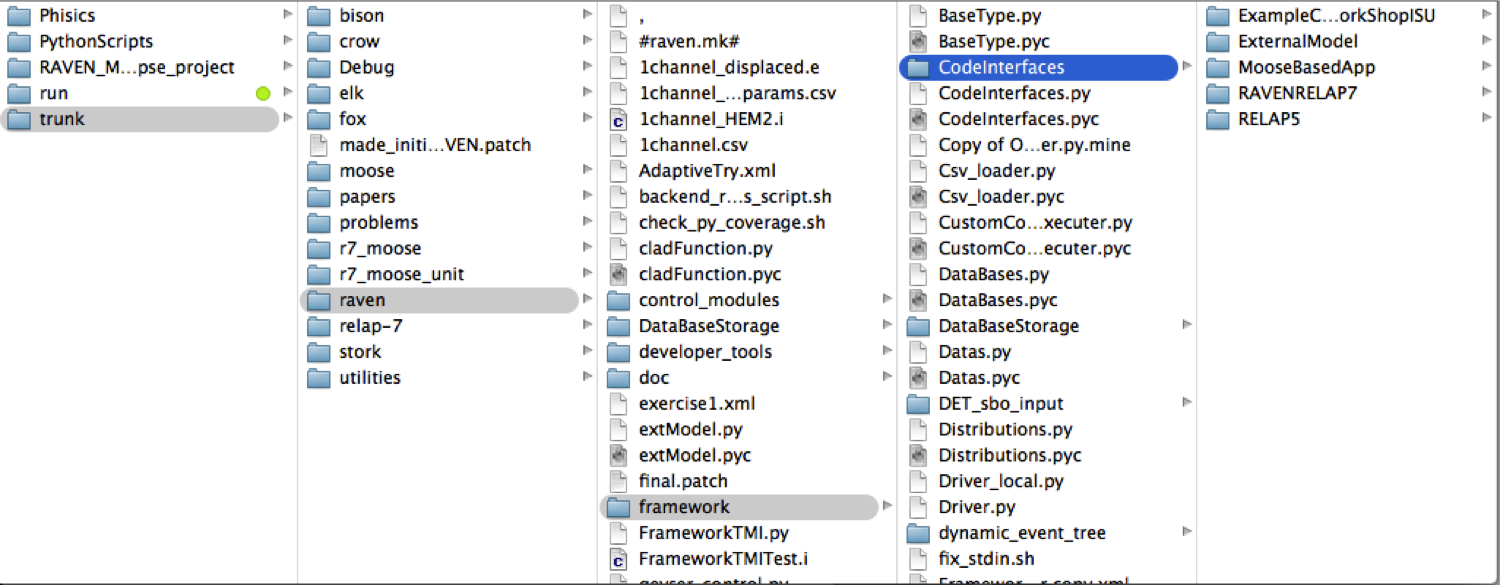
\includegraphics[width=1.0\textwidth]{pics/CodeInterfaceLocation.png}
\caption{Code Interface Location.}
\label{fig:codeinterface}
\end{figure}
The procedure of coupling a new code/application with RAVEN is a straightforward process.
For all the codes currently supported by RAVEN (e.g. RELAP-7, RELAP5-3D,
BISON, MOOSE,etc.), the coupling is performed through a Python interface that interprets the information coming from RAVEN and translates them into the
  input of the driven code.
The coupling procedure does not require modifying RAVEN itself. Instead, the developer creates a new Python interface that is going to be embedded
 in RAVEN at run-time (no need to introduce  hard-coded coupling statements).
 This interface needs to be placed in a folder (whatever name) located in (see figure~\ref{fig:codeinterface}):
\begin{lstlisting}[language=bash]
 path/to/raven/distribution/raven/framework/CodeInterfaces/
\end{lstlisting}
At the initialization stage, RAVEN imports all the Interfaces that are contained in this directory and performs some preliminary cross-checks.
\\It is important to notice that the name of class in the Interface module is the one the user needs to specify when the new interface
needs to be used. For example, if the Interface module contains the class 	``NewCode'', the \textit{subType} in the \xmlNode{Code} block will be 	``NewCode'':
\begin{lstlisting}[language=python]
  class NewCode(CodeInterfaceBase):
    ...
\end{lstlisting}
\begin{lstlisting}[style=XML,morekeywords={name,file}] %moreemph={name,file}]
  <Models>
    ...
    <Code name='whatever' subType='NewCode'>
     ...
    </Code>
    ...
  </Models>
\end{lstlisting}
In the following sub-sections, a step-by-step procedure for coupling a code to RAVEN is outlined.
\subsection{Pre-requisites.}
\label{subsec:prerequisites}
In order to couple a newer application to the RAVEN code, some pre-requisites need to be satisfied.
%%% INPUT %%%
\newline
\\\textbf{\textit{\underline{Input}}}
\newline
\\ The first pre-requisite is the knowledge of the input
syntax of the application the developer wants to couple. Indeed, RAVEN task
 ``ends'' at the Code Interface stage. RAVEN transfers the information needed
 to perturb the input space into the Code interface and expects that the newly
 developed Interface is able to perturb the input files based on the information
 passed through.
\\This means that the developer needs to code a Python-compatible parser of
 the system code input (a module that is able to read and modify the input of
 the code that needs to be coupled).
\\ For example, let's suppose the input syntax of the code the developer needs
to couple is as follows:
\begin{lstlisting}[language=python]
  kewword1 =  aValue1
  kewword2 =  aValue2
  kewword3 =  aValue3
  kewword4 =  aValue4
\end{lstlisting}
The Python input parser would be:
\begin{lstlisting}[language=python]
class simpleInputParser():
  def __init__(self,filename):
    #
    # @ In, string, filename, input file name (with path)
    #
    self.keywordDictionary = {}
    # open the file
    fileobject = open(filename)
    # store all the lines into a list
    lines = fileobject.readlines()
    # parse the list to construct
    # self.keywordDictionary dictionary
    for line in lines:
      # split the line with respect
      # to the symbol "=" and store the
      # outcomes into the dictionary
      # listSplitted[0] is the keword
      # listSplitted[1] is the value
      listSplitted = line.split("=")
      keyword = listSplitted[0]
      value   = listSplitted[1]
      self.keywordDictionary[keyword] = value
    # close the file
    fileobject.close()

  def modifyInternalDictionary(self,inDictionary):
      #
      # @ In, dictionary {keyword:value},
      # inDictionary, dictionary containing
      # the keywords to perturb
      #

    # we just parse the dictionary and replace the
    # matching keywords
    for keyword,newvalue in inDictionary.items():
      self.keywordDictionary[keyword] = newvalue

  def writeNewInput(self,filename):
    #
    # @ In, string, filename, newer input file name (with path)
    #

    # open the file
    fileobject = open(filename)
    # write line by line
    for keyword,newvalue in self.keywordDictionary.items():
      fileobject.write(keyword + ``='' + str(newvalue) + ``\n'')
    # close the file
    fileobject.close()
\end{lstlisting}
It is important to notice that for most of the codes, a wild-card approach can be used. In case this approach fits the user's needs,
the RAVEN developer team suggests to inherit from the $GenericCode$ Interface (see section ~\ref{subsec:genericInterface}).

%%% OUTPUT %%%
\textbf{\textit{\underline{Output}}}
\newline
\\RAVEN is able to handle Comma Separated Value (CSV) files (as outputs
of the system code). In order make RAVEN able to retrieve the information
 from the newly coupled code, these files need to be  either generated by the
 system code itself or the developer needs to code a Python-compatible
module to convert the whatever code output format to a CSV one.
This module can be  directly called in the new code interface (see following section).
\\ Let's suppose that the output format of the code (the same of the previous
input parser example) is as follows:
\begin{lstlisting}[language=python]
  result1 = aValue1
  result2 = aValue2
  result3 = aValue3
\end{lstlisting}
The Python output converter would be as simple as:
\begin{lstlisting}[language=python]
def convertOutputFileToCSV(outputfile):
    keywordDictionary = {}
    # open the original file
    fileobject = open(outputfile)
    outputCSVfile = open (outputfile + '.csv')
    # store all the lines into a list
    lines = fileobject.readlines()
    # parse the list to construct
    # self.keywordDictionary dictionary
    for line in lines:
      # split the line with respect
      # to the symbol "=" and store the
      # outcomes into the dictionary
      # listSplitted[0] is the keword
      # listSplitted[1] is the value
      listSplitted = line.split("=")
      keyword = listSplitted[0]
      value   = listSplitted[1]
      keywordDictionary[keyword] = value
    outputCSVfile.write(','.join(keywordDictionary.keys()))
    outputCSVfile.write(','.join(keywordDictionary.values()))
    outputCSVfile.close()
\end{lstlisting}
And the output CSV becomes:
\begin{lstlisting}[language=python]
  result1, result2, result3
  aValue1, aValue2, aValue3
\end{lstlisting}
Note that in general RAVEN is content with accepting floats or strings as data types in the CSV.
However, if the CSV produced by running the code has a large number of columns (say, over 1000), it
is necessary to include only floats and change the CSV loading utility. See more below (\ref{subsubsec:setCsvLoadUtil})
%%%%%%%
\subsection{Code Interface Creation}
\label{subsec:codeinterfacecreation}
As already mentioned, RAVEN imports all the ``Code Interfaces'' at run-time,
without actually knowing the syntax of the driven codes. In order to make RAVEN
able to drive a newer software, the developer needs to code a Python module
that will contain few methods (with strict syntax) that are called by RAVEN during the simulation.
\\ When loading a ``Code Interface'', RAVEN expects to find, in the class representing the code,
 the following required methods:
\begin{lstlisting}[language=python]
from CodeInterfaceBaseClass import CodeInterfaceBase
class NewCode(CodeInterfaceBase):
  def generateCommand(self, inputFiles, executable, clargs=None, fargs=None, preExec=None)
  def createNewInput(self, currentInputFiles, oriInputFiles,
                                samplerType, **Kwargs)
\end{lstlisting}
In addition, the following optional methods can be specified:
\begin{lstlisting}[language=python]
from CodeInterfaceBaseClass import CodeInterfaceBase
class NewCode(CodeInterfaceBase):
  ...
  def initialize(self, runInfoDict, oriInputFiles)
  def finalizeCodeOutput(self, command, output, workingDir)
  def getInputExtension(self)
  def checkForOutputFailure(self, output, workingDir)
\end{lstlisting}
In the following sub-sections all the methods are fully explained, providing examples
 (referring to the simple code used as example for the previous sections)
\subsubsection{Method: \texttt{generateCommand}}
\label{subsubsec:generateCommand}
\begin{lstlisting}[language=python]
def generateCommand(self, inputFiles, executable, clargs=None, fargs=None, preExec=None)
\end{lstlisting}
The \textbf{generateCommand} method is used to generate the commands
(in \texttt{string} format) needed to launch the driven Code, as well as the root name of the output of the perturbed inputs (in \texttt{string} format).
The return for this command is a two-part \texttt{Python} tuple.  The first entry is a list of two-part tuples, each
which specifies whether the corresponding command
should be run exclusively in serial, or whether it can be run in parallel, as well as the command itself.
For example, for a command where
two successive commands are called, the first in serial and the second in parallel,

\begin{lstlisting}[language=python]
  def generateCommand(self,inputFiles,executable,clargs=None,fargs=None, preExec=None):
    . . .
    commands = [('serial',first_command), ('parallel',second_command)]
    return (commmands,outFileRoot)
\end{lstlisting}
For each command, the second entry in the tuple is a string containing the full command
that the internal JobHandler is going to use to run the Code this interface refers to.
The return data type must be a Python \texttt{tuple} with a list of tuples and a string: (\texttt{commands, outfileRoot}).
Note that in most cases, only a single command needs to be run, so only a single command tuple is necessary.
At run time, RAVEN will string together commands attached by double ampersands (\&\&), and each command
labeled as parallel-compatible will be prepended with appropriate mpi arguments.  For the example above, the
command executed will be (with \xmlNode{NumMPI} equal to 4)

\begin{lstlisting}[language=bash]
$  first_command && mpiexec -n 4 second_command
\end{lstlisting}

RAVEN is going to call the \texttt{generateCommand} function passing in the following arguments:
\begin{itemize}
  \item \textbf{\texttt{inputFiles}}, data type = list: List of input files (length of the list depends on the
           number of inputs listed in the Step which is running this code);
  \item \textbf{\texttt{executable}}, data type = string, executable name with absolute
            path \\(e.g. /home/path\_to\_executable/code.exe);
  \item  \textbf{\texttt{clargs}}, \emph{optional}, data type = dictionary, a dictionary containing the command-line flags the
               user can specify in the input (e.g. under the node $<Code><clargs type='input' arg='-i' extension='.inp'/></Code>$).
  \item  \textbf{\texttt{fargs}}, \emph{optional}, data type = dictionary, a dictionary containing the axuiliary input file variables the
               user can specify in the input (e.g. under the node $<Code><clargs type='input' arg='aux' extension='.aux'/></Code>$).
             \item \textbf{\texttt{preExec}}, \emph{optional}, data type = string, a string the command that needs to be
               pre-executed before the actual command. The user can specify in the input
               (e.g. under the node $<Code><preexec>pre-execution command</preexec></Code>$)
               \default{None}
\end{itemize}
For the example referred to in the previous section, this method would be implemented as follows:
\newline
\begin{lstlisting}[language=python]
  def generateCommand(self,inputFiles,executable,clargs=None,fargs=None, preExec=None):
    found = False
    for index, inputFile in enumerate(inputFiles):
      if inputFile.endswith(self.getInputExtension()):
        found = True
        break
    if not found: raise IOError(
          `None of the input files has one of the following extensions: ` +
           ` `.join(self.getInputExtension()))
    outputfile = 'out~'+os.path.split(inputFiles[index])[1].split('.')[0]
    executeCommand = [('parallel',executable+ ` -i ` +os.path.split(inputFiles[index])[1])]
    return executeCommand,outputfile
\end{lstlisting}


\subsubsection{Method: \texttt{createNewInput}}
\label{subsubsec:createNewInput}
\begin{lstlisting}[language=python]
def createNewInput(self,currentInputFiles,oriInputFiles, samplerType,**Kwargs)
\end{lstlisting}
The \textbf{createNewInput} method is used to generate an input based
on the information RAVEN passes in. In this function the developer needs to
call the driven code input parser in order to modify the input file, accordingly with
respect to the variables RAVEN is providing. This method needs to return a list containing
the path and filenames of the modified input files. \nb RAVEN expects that at least one input
file of the original list gets modified.

RAVEN is going to call this function passing in the following arguments:
\begin{itemize}
  \item \textbf{\texttt{currentInputFiles}}, data type = list: List of current
              input files. This list of files is the one the code interface needs to use to print the new perturbed list of files.
              Indeed, RAVEN already changes the file location in sub-directories and the Code Interface does not need to
              change the filename or location of the files. For example, the files are going to have a absolute path as following:
              $.\\ path\_to\_working\_directory\\stepName\\anUniqueIdentifier\\filename.extension$. In case of sampling, the
              ``\textit{anUniqueIdentifier}'' is going to be an integer (e.g. 1).
  \item \textbf{\texttt{oriInputFiles}} , data type = list, List of the original input files;
  \item  \textbf{\texttt{samplerType}} , data type = string, Sampler type (e.g. MonteCarlo,
               Adaptive, etc.). \nb None if no Sampler has been used;
  \item  \textbf{\texttt{Kwargs}} , data type = kwarded dictionary, dictionary of parameters.
               In this dictionary there is another dictionary
               called "SampledVars" where RAVEN stores the
               variables that got sampled
               (Kwargs['SampledVars'] = \{'var1':10,'var2':40\});
\end{itemize}
For the example referred in the previous section, this method would implemented as follows:
\newline
\begin{lstlisting}[language=python]
  def createNewInput(self,currentInputFiles,
        oriInputFiles,samplerType,**Kwargs):
    for index, inputFile in enumerate(oriInputFiles):
      if inputFile.endswith(self.getInputExtension()):
        break
    parser = simpleInputParser(currentInputFiles[index])
    parser.modifyInternalDictionary(**Kwargs['SampledVars'])
    parser.writeNewInput(newInputFiles[index])
    return newInputFiles
\end{lstlisting}


\subsubsection{Method: \texttt{getInputExtension}}
\label{subsubsec:getInputExtension}
\begin{lstlisting}[language=python]
def getInputExtension(self)
\end{lstlisting}
The \textbf{getInputExtension} function is an optional method. If present, it is called
by RAVEN code at run time.  This function can be considered an utility method, since its
main goal is to return a tuple of strings, where the developer can place all the input extensions
the code interface needs to support (i.e. the extensions of the input(s) the code interface
is going to ``perturb''). If this method is not implemented, the default extensions are  \textbf{(".i", ".inp", ".in"')}.
This function does not accept any input argument.
For the example referred in the previous section, this method would implemented as follows:
\newline
\begin{lstlisting}[language=python]
def getInputExtension(self):
    return (".i",".input")
\end{lstlisting}

\subsubsection{Method: \texttt{initialize}}
\label{subsubsec:codeInterfaceinitialize}
\begin{lstlisting}[language=python]
def initialize(self, runInfoDict, oriInputFiles)
\end{lstlisting}
The \textbf{initialize} function is an optional method. If present, it is called
by RAVEN code at the begin of each Step (once per step) involving the particular Code Interface.
This method is generally indicated to retrieve information from the RunInfo and/or the Input files.
\\RAVEN is going to call this function passing in the following arguments:
\begin{itemize}
  \item \textbf{\texttt{runInfoDict}}, data type = dictionary: dictionary of the info stored in the run info XML block;
  \item \textbf{\texttt{oriInputFiles}}, data type = list, list of the original input files.
\end{itemize}


\subsubsection{Method: \texttt{finalizeCodeOutput}}
\label{subsubsec:finializeCodeOutput}
\begin{lstlisting}[language=python]
def finalizeCodeOutput(self, command, output, workingDir)
\end{lstlisting}
The \textbf{finalizeCodeOutput} function is an optional method. If present, it is called
by RAVEN code at the end of each run. It can be used for those codes, that do not create CSV
files as output to convert the whatever output format into a CSV. RAVEN checks if a string is returned;
if so, RAVEN interprets that string as the new output file name (CSV).
\\RAVEN is going to call this function passing in the following arguments:
\begin{itemize}
  \item \textbf{\texttt{command}}, data type = string: the command used to run
                    the just ended job;
  \item \textbf{\texttt{output}}, data type = string, the Output name root;
  \item  \textbf{\texttt{workingDir}}, data type = string, current working directory.
\end{itemize}
For the example referred in the previous section, this method would implemented as follows:
\newline
\begin{lstlisting}[language=python]
def finalizeCodeOutput(self, command, output, workingDir):
    outfile = os.path.join(workingDir,output+".o")
    convertOutputFileToCSV(outfile)
 \end{lstlisting}

 \subsubsection{Method: \texttt{checkForOutputFailure}}
\label{subsubsec:checkForOutputFailure}
\begin{lstlisting}[language=python]
def checkForOutputFailure(self, output, workingDir)
\end{lstlisting}
The \textbf{checkForOutputFailure} function is an optional method. If present, it is called
by RAVEN code at the end of each run. This method needs to be implemented by the codes that, if a run fails, return a ``returncode'' = 0.
This can happen in those codes that record the failure of a run (e.g. not converged, etc.) as normal termination (returncode == 0)
This method can be used, for example, to parse the outputfile looking for a special keyword that testifies that a particular job  failed
 (e.g. in RELAP5 would be the keyword "********"). This method MUST return a boolean (True if failed, False otherwise).
\\RAVEN is going to call this function passing in the following arguments:
\begin{itemize}
  \item \textbf{\texttt{output}}, data type = string,the Output name root;
  \item  \textbf{\texttt{workingDir}}, data type = string, current working directory.
\end{itemize}
For the example referred in the previous section, this method would implemented as follows:
\newline
\begin{lstlisting}[language=python]
def checkForOutputFailure(self, command, output, workingDir):
    from  __builtin__ import any
    errorWord = "ERROR"
    return any(errorWord in x for x in
      open(os.path.join(workingDir,output+'.o'),"r").readlines())
 \end{lstlisting}

\subsubsection{Method: \texttt{setRunOnShell}}
\label{subsubsec:setRunOnShell}
\begin{lstlisting}[language=python]
self.setRunOnShell(shell=True)
\end{lstlisting}
The \textbf{setRunOnShell} function is an optional method. The default for shell is ``True''.
In RAVEN, the \textit{subprocess} module from Python is used to spawn new processes, connect
to their input/output/error pipes, and obtain their return codes. To support a wide variety of
use cases, the \textit{Popen} constructor from \textit{subprocess} is used to accept a large number
of optional arguments. For most typical use cases, RAVEN will set these arguments automatically,
and the code interface developers should not worry about the values for these arguments. However, in
some specific use cases, the following argument may need to be setted by the code interface developers:
\begin{itemize}
  \item{shell}, the default value is \textbf{True}. If shell is \textbf{True}, the specified command
    generated by RAVEN will be executed through the shell. This will allow RAVEN to have an enhanced
    control flow with convenient access to other shell features such as shell pipes, filename wildcards,
    environment variable expansion, and expansion of ``~'' to a user's home directory. If shell is
    \textbf{False}, all the shell based features are disabled. In other words, the users could not use the
    shell features in the code inteface to generate the commands that are needed to lauch the driven code,
    i.e. the \textbf{generateCommand} method mentioned before should not use any shell features when constructs
    the commands. For more detailed description, please refer to the Python subprocess page
    \url{https://docs.python.org/2/library/subprocess.html}
    \nb If external codes can not run through ``Shell'', the code interface developers should call this
    function with ``shell=False'' in the ``\_\_init\_\_'' method. For example:
    \begin{lstlisting}[language=python,showstringspaces=false]
    def __init__(self):
      self.setRunOnShell(shell=False)
    \end{lstlisting}
\end{itemize}

\subsubsection{Method: \texttt{setCsvLoadUtil}}
\label{subsubsec:setCsvLoadUtil}
\begin{lstlisting}[language=python]
self.setCsvLoadUtil('pandas')
\end{lstlisting}
The default CSV loader in RAVEN is pandas, which allows arbitrary data types in the CSV, generally
strings and floats. However, arbitrary data can be challenging to load if there are a large number
of columns in the code's output CSV that RAVEN attempts to read in. As a rule of thumb, if there are
over 1000 columns in a typical output CSV for your Code, the resulting values should only be floats
and integers (not strings), and this method should be called during the CodeInterface construction
or initialization
to set the loading utility to \texttt{numpy}. While RAVEN's \texttt{numpy} CSV loading is notably
faster than RAVEN's \texttt{pandas} CSV loading, it does not allow the flexibility of string entries
except in the CSV header.

\subsection{Tools for Developing Code Interfaces}
To make generating a code interface as simple as possible, there are several tools RAVEN makes available within the Code Interface objects.

\subsubsection{File Objects}
RAVEN has created a wrapper for files within Python in order to carry along some additional information.  This allows the user to tag particular files for reference in the Code Interface, using the \xmlAttr{type} XML attribute in \xmlNode{Files} nodes.  To differentiate, RAVEN file objects will use the capital Files, whereas typical files will use the lowercase files.

When the Files are passed in to \texttt{createNewInput}, they are passed in as Files objects. To access the xmlAttr{type} of a file, use the method \texttt{getType}.  For instance, instead of looking for an extension, a Code Interface might identify an input file by looking for a particular type, as shown in the example below. \nb RAVEN does not access a File's \xmlAttr{type}; it is exclusively an optional tool for Code Interface developers.

\begin{lstlisting}[language=python,showstringspaces=false]
found = False
for inFile in inputFiles:
  if inFile.getType()=='mainInput':
    found = True
    break
if not found:
  raise IOError('Desired file with type ``mainInput'' not found!')
\end{lstlisting}
Using Files \xmlAttr{type} attributes can especially help when multiple input files have the same extension.  For example, say a Code execution command normally has the following appearance on the command line:
\begin{lstlisting}[language=bash]
/home/path/to/executable/myexec.sh -i mainInp.xml -a auxInp.xml --mesh cube.e
\end{lstlisting}
The \xmlNode{Files} block in the RAVEN XML might appear as follows:
\begin{lstlisting}[language=XML]
<Files>
  <Input name='main' type='base'>mainInp.xml</Input>
  <Input name='two'  type='aux' >auxInp.xml</Input>
  <Input name='cube' type='mesh' perturbable='False'>cube.e</Input>
</Files>
\end{lstlisting}
The search for these files in the Code Interface might then look like the example below, assuming one file per type:
\begin{lstlisting}[language=python,showstringspaces=false]
# populate a type dictionary
typesDict={}
for inFile in inputFiles:
  typesDict[inFile.getType()]=inFile
# check all the necessary files are there
if 'base' not in typesDict.keys():
  raise IOError('File type ``base'' not listed in input file!')
if 'aux' not in typesDict.keys():
  raise IOError('File type ``aux'' not listed in input file!')
if 'mesh' not in typesDict.keys():
  raise IOError('File type ``mesh'' not listed in input file!')
mainFile = typesDict['base']
# do operations on file, etc.
\end{lstlisting}

Additionally, a Code Interface developer can access the \xmlAttr{perturbable} through the \texttt{getPerturbable()} method of a Files object.  This can be useful, for example, in preventing searching binary files for variable names when creating new input. For example,
\begin{lstlisting}[language=python]
for inFile in inputFiles:
  if not inFile.getPerturbable(): continue
  # etc
\end{lstlisting}

\section{Advanced Users: How and When to create a RAVEN Template}
\label{sec:newTemplate}

One of the great strengths of the RAVEN input is its flexibility; an enormous number of different types of workflows can
%
be constructed with the components outlined in this manual. Sometimes, this flexibility is not required when standard or
%
predefined workflows need to be employed changing just few settings. For example, in classical uncertainty
%
quantification, sometimes only a few variables or the model needs to be changed, while the rest of the workflow stays
%
the same.
\\

As a tool to focus RAVEN on particular workflows, we introduce the RAVEN Templated Input Files. The intention of this
%
system is to allow a single user to develop a template RAVEN input file along with a template interface, thereby
%
simplifying inputs for any number of users that only need to make minor changes to the templated workflow in order to
%
perform their analysis.
\\

\nb A RAVEN Template is a wrapper for creating RAVEN input files; it is not part of the RAVEN core code and is usually s
%
specific to a particular application.

\subsection{When to use a RAVEN Template}
%
By design, a RAVEN Template simplifies the user experience at the cost of flexibility. The amount of streamlining is
%
adjustable and specific to each template. At one extreme, a Template takes no modifications at all and always produces
%
the same workflow; at the other extreme the Template duplicates entirely the RAVEN input syntax. Neither of those
%
options is desirable; Templates should find ground in-between.
\\

There are some times where using a RAVEN Template can be highly beneficial:
%
\begin{itemize}
  \item The workflow in question is highly complex, involving some advanced RAVEN usage to perform unorthodox calculations,
  %
  \item The workflow is mostly the same for each user, requiring only a small number of changes to use repeatedly.
\end{itemize}

There are some times when using a RAVEN Template is unlikely to be useful:
%
\begin{itemize}
  \item The workflow needs to be flexible enough to accommodate many unpredictable changes,
  %
  \item The workflow has few entries and can be changed manually quite easily.
\end{itemize}

\subsection{How to create a RAVEN Template}
%
A RAVEN Template consists of three main pieces: a Templated Workflow, a Template Class, and a Template Interface. The
%
Interface is the main driver, and uses an input file to inform the Template Class on how to modify the Templated
%
Workflow in order to create a new RAVEN input file.

\begin{figure}[h!]
 \centering
 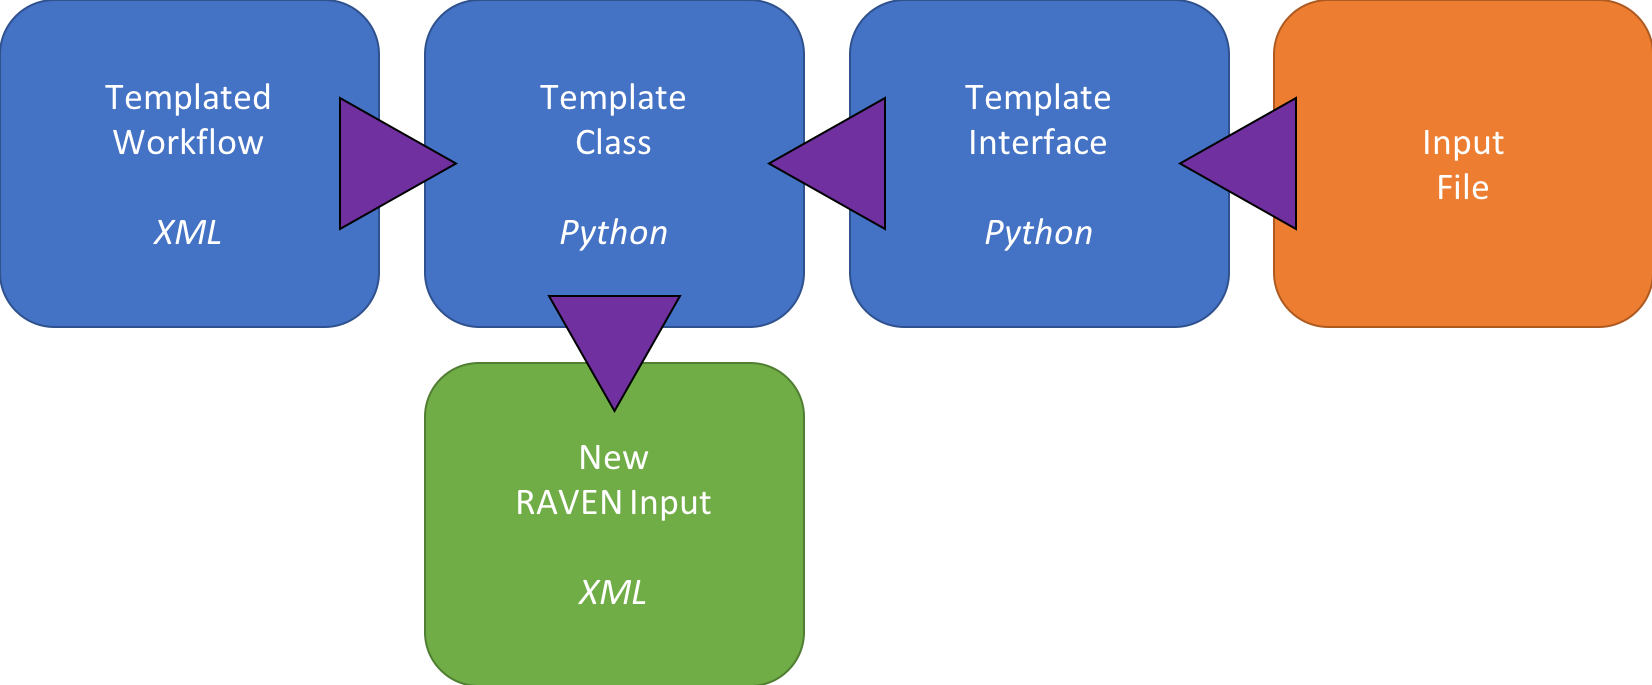
\includegraphics[width=\textwidth]{pics/TemplateWorkflow.png}
 \caption{Information Flow for RAVEN Templates}
 \label{fig:raven template workflow}
\end{figure}

Refer to Figure \ref{fig:raven template workflow}. Each box represents a file in a RAVEN template system. The three
%
boxes in blue (Templated Workflow, Template Class, and Template Interface) are developed collectively as the Template
%
by a designer familiar with RAVEN input files and Python. The development of this template only needs to occur once. The
%
orange box (Input File) is in a format determined by the Template Interface, and is the only portion of the Template
%
that a user will interact with repeatedly for any given workflow. The green box (New RAVEN Input) is the result of
%
reading a particular input file with the Template and is written by the Template. This new input can either be run
%
automatically with RAVEN or left to run at the user's convenience, based on what the Template Interface is designed to
%
do. Note that running RAVEN from within a python script on Windows within MinGW is particularly tricky.
\\

The three portions of the Template are discussed individually in the following sections.

\subsubsection{Templated Workflows}
%
A Templated Workflow begins with a traditional RAVEN input file that is run to do a particular analysis. It is highly
%
recommended that this workflow is run with RAVEN and the inputs and outputs are well understood before beginning
%
templating. Keep a copy of the original workflow before modifying the Templated Workflow.
\\

Next, consider the parts of the workflow that are common to anyone who will want to perform a similar analysis, and
%
which are specific to individual runs. For example, perhaps the \xmlNode{Sequence} and \xmlNode{Steps} are always the
%
same, but the \xmlNode{Model} and sampled \xmlNode{variable} nodes may change for each analysis. Note those parts of the
%
original workflow that need to be flexible, and remove them from the Templated Workflow. These will be filled in by the
%
Template Class for this workflow when the Template Interface is run.



\subsubsection{Template Class}
%
The Template Class is a bridge between the template designer and the Templated Workflow. The Template Class knows every
%
detail about the Templated Workflow and knows how to modify it to create a working RAVEN input.  It does so through a
%
set of standardized calls from the Template Interface.

A Template Base Class is provided in the RAVEN repository to be inherited by your new Template Class. It is located in
%
\begin{lstlisting}[language=bash]
 raven/framework/InputTemplates/TemplateBaseClass.py
\end{lstlisting}
%
We recommend you locate your new Template Class near your project where the workflows are run, and not in the RAVEN
%
repository.

There are several required methods in the API of the Template Base Class that are important.
%
\begin{lstlisting}[language=python]
 loadTemplate(self, filename, path)
\end{lstlisting}
%
The \texttt{loadTemplate} method is how the Template Class knows how to load the Template Workflow. The default
%
implementation in the Template Base Class is probably sufficient for most Template Classes, where given the filename and
%
path to the file, the template is loaded into \texttt{self.\_template}. Of course, this behavior can be modified however
%
suits a project by overloading this method in the Template Class.

\begin{lstlisting}[language=python]
 createWorkflow(self, **kwargs)
\end{lstlisting}
%
The \texttt{createWorkflow} method is the main method of the Template Class. The Template Interface calls this method
%
when it wants to use a series of modifications to write a new RAVEN input file. Note the Template Base Class
%
implementation of \texttt{createWorkflow} accepts arbitrary keyword arguments as \texttt{**kwargs}. This allows the
%
inheriting Template Class to define its own required arguments necessary to write a new input file. These may be lists,
%
dictionaries, or any other Python object. All of the necessary information for the Template Class to convert a Template
%
Workflow into a valid RAVEN input file should be passed through these arguments.
\\

The rest of \texttt{createWorkflow} is open to do any operations necessary to modify the XML in the Template Workflow
%
until it becomes a valid RAVEN input that performs the desired analysis. RAVEN offers a plethora of handy XML tools in
%
\texttt{raven/framework/xmlUtils}, which is imported in the base class and can be imported in your Template Class as
%
well. In addition, the Python standard library has an excellent \texttt{xml.etree.ElementTree} package for manipulating
%
XML.  Note that any \texttt{createWorkflow} should start by deepcopying the template XML, to assure a clean copy is
%
available each time it is called. The \texttt{createWorkflow} ends by returning the modified XML element.

\begin{lstlisting}[language=python]
 writeWorkflow(self, template, destination, run=False)
\end{lstlisting}
%
Once \texttt{createWorkflow} is called, the resulting XML element can be supplied to the \texttt{writeWorkflow} method,
%
which writes the XML to a file. The Template Base Class implementation will likely cover the needs of most Template
%
Classes, and shouldn't require significant modification. Note that an optional argument \texttt{run} instructs the
%
Template Class to attempt to run the workflow in RAVEN once it is written to file. Note this currently works on Mac
%
and Linux systems, but is not yet consistent on Windows.
\\

Other optional methods also exist in the Template Base Class and may be of use to individual templates.
%
\begin{lstlisting}[language=python]
 addNamingTemplates(cls, templates)
\end{lstlisting}
%
Note that the Template Base Class has a class-level dictionary member called \texttt{namingTemplates}. The intention of
%
this method is to store common ways to name items in the RAVEN input in a format method so that later they are always
%
consistent. To extend this method, call \texttt{BaseClass.addNamingTemplates} at the class level in the inheriting
%
Template Class.
\\

Finally, commonly-used shortcuts are included at the end of the Template Base Class to perform actions that are
%
repetitively used in modifying RAVEN inputs. We recommend you add your own to your Template Class to help keep
%
\texttt{createWorkflow} clean and easily maintainable.



\subsubsection{Template Interface}
%
The Template Interface is the code that actually gets called by users once the Template Class and Template Workflow are
%
complete. In its simplest form, the Template Interface is a Python script that reads the data needed for the
%
\texttt{createWorkflow} method and calls the methods on the Template Class in order:
%
\begin{enumerate}
  \item \texttt{loadTemplate}
  \item \texttt{createWorkflow}
  \item \texttt{writeWorkflow}
\end{enumerate}
%
Template Interfaces read a simplified input file so that users can provide their parameters for the Templated Workflow
%
in an easy manner. Whatever enables the use of the RAVEN workflow with minimal effort on the part of the users is ideal
%
for the Template Interface.





\subsection{Example}
%
For testing and as an example of implementation, a simple Template was created to perform basic uncertainty
%
quantification (UQ) analysis on external models. The example can be found in
%
\begin{lstlisting}[language=bash]
 raven/tests/framework/TemplateInputs
\end{lstlisting}
%
The following files are part of this template under the directory given above:
%
\begin{itemize}
  \item Templated Workflow: \texttt{TemplateInputs/UQTemplate/uq\_template.xml}
  %
  \item Template Class: \texttt{TemplateInputs/UQTemplate/UQTemplate.py}
  %
  \item Template Interface: \texttt{TemplateInputs/uq\_maker.py}
  %
  \item Input File: \texttt{TemplateInputs/UQTemplate/uq\_template\_input.i}
\end{itemize}
%
The original workflow from which the Templated Workflow was created involved a simple Monte Carlo sampling of an
%
external model and then postprocessing with BasicStatistics to find the mean, standard deviation, skewness, and kurtosis
%
of the results. The Template designer determined that this workflow could be used for many similar analyses with only
%
small changes, and decided to template it. The designer determined that things that could be changed include the model
%
sampled, the outputs of the model, the inputs to the model (with their distributions), and the number of Monte Carlo
%
samples to take. The designer also decided that each case should have its own WorkingDir to keep analyses separate. We
%
will consider the resulting Template files that the designer wrote one at a time in the following sections.



\subsubsection{Example Templated Workflow}
%
The file \texttt{uq\_template.xml} looks much like a typical RAVEN input file with some key pieces missing. The
%
\xmlNode{Sequence} shows that the two steps are \xmlString{sample} and \xmlString{stats}, which are for sampling a model
%
using Monte Carlo sampling and then performing some statistics on the results. Note however the missing contents in the
%
\xmlNode{WorkingDir}, the empty nodes in the \xmlNode{DataObjects}, the lack of any \xmlNode{Distributions}, and the
%
missing variable lists in the xmlNode{PostProcessor}. All the missing contents are filled in by the Template Class. For
%
the results of the filled-in workflow, see in
%
\begin{lstlisting}[language=bash]
 raven/tests/framework/TemplateInputs/gold/UQTemplate/new_uq.xml
\end{lstlisting}



\subsubsection{Example Template Class}
%
The file \texttt{UQTemplate.py} demonstrates inheritance of the Template Base Class and customization for the logic to
%
fill in the Templated Workflow.
\\

Note that the Template Class adds three formatted strings to the class-level name templates, one each for step names,
%
distributions, and metric variables. These are called later in the code to assure the naming conventions are always the
%
same. These formatted strings employ Python's inherent string formatting tools.
\\

The Template Base Class implementation of \texttt{loadWorfklow} does everything this Template needs to load the
%
Templated Workflow, so there is no need to modify it in the custom Template Class. Similarly, the \texttt{writeWorkflows}
%
does everything this Template needs to write a newly-created input, so there is no need to modify it in the custom
%
Template Class.  Since there was no need to overload the Template Base Class implementations of \texttt{loadWorfklow}
%
and \texttt{writeWorkflows}, the only main method changed in the Template Class is the essential \texttt{createWorkflow}
%
method. Note that we've added several keywords to the argument list:
%
\begin{lstlisting}[language=python]
  def createWorkflow(self, model=None, variables=None, samples=None, case=None, **kwargs):
\end{lstlisting}
%
In order to correctly modify the Templated Workflow, the Template Class needs to know about what model is being sampled,
%
the input variables to the model and how they're distributed, how many Monte Carlo samples to take, and the name of the
%
case being run. It requires all of these to be provided by the Template Interface in order to write a new RAVEN input.
%
In this case, the method arguments \texttt{model} and \texttt{variables} are dictionaries, while the \texttt{samples}
%
are an integer and the \texttt{case} is a string.
\\

Note that \texttt{UQTemplate.createWorkflow} calls the Template Base Class's implementation first in order to preserve
%
inheritance. Since the deepcopy happens in the base class, we don't perform it again in the custom Template Class.
\\

Throughout the remainder of the workflow creation, a series of XML manipulations are performed based on the inputs
%
provided from the Template Interface. For example, the module to load for the Model is changed, the working directory is
%
set, and the input and output variables are propagated throughout the input file. Note also that several input
%
construction shortcut methods have been added for this particular template to simplify maintenance of the template.


\subsubsection{Example Template Interface}
%
The file \texttt{uq\_maker.py} contains the basic logic needed to read a user input file, load the Template Class, and
%
generate new inputs. It follows the sequence of events outlined above, first instructing the Template Class to load the
%
template, then reading in the user input, then instructing the Template Class to create the workflow, then to write the
%
workflow.
\\

Beause the input needs for this Template are simple, we use Python's standard library \texttt{configparser} to read in
%
the user input file, \texttt{uq\_template\_input.i}. This simple input structure uses sections (model, variables, and
%
settings) with keyword and value pairs in each section. In order to change the RAVEN workflow created, the user only
%
needs to make changes to the existing input file and run the interface, then run RAVEN on the new input.
\\

Note that we chose to provide the information to the Template Class mostly through dictionaries, where the essential
%
pieces of information can be provided. In particular note that the variables provide only a mean and standard deviation;
%
one reduction in flexibility is that we assume the variables are normally distributed, disallowing other distributions.
\\

The Template can be run with Python from the command line:
%
\begin{lstlisting}[language=bash]
 > python uq_maker.py
 > cd UQTemplate
 > ~/projects/raven/raven_framework new_uq.xml
\end{lstlisting}
%
It reads in the user input, modifies the template, writes the new input file, and finally runs RAVEN. Note that, if
%
desired, the interface can be extended to perform additional operations after RAVEN has finished creating the workflow.

\appendix
\section{Appendix: Example Primer}
\label{sec:examplePrimer}
In this Appendix, a set of examples are reported. In order to be as general as possible, the \textit{Model} type ``ExternalModel'' has been used.
%%%% EXAMPLE 1
\subsection{Example 1.}
\label{subsec:ex1}
This simple example is about the construction of a ``Lorentz attractor'', sampling the relative input space. The parameters that are sampled represent the initial coordinate (x0,y0,z0) of the attractor origin.

\begin{lstlisting}[style=XML,morekeywords={debug,re,seeding,class,subType,limit}]
<?xml version="1.0" encoding="UTF-8"?>
<Simulation verbosity="debug">
<!-- RUNINFO -->
<RunInfo>
    <WorkingDir>externalModel</WorkingDir>
    <Sequence>FirstMRun</Sequence>
    <batchSize>3</batchSize>
</RunInfo>
<!-- Files -->
<Files>
    <Input name='lorentzAttractor.py' type=''>lorentzAttractor</Input>
</Files>
<!-- STEPS -->
<Steps>
    <MultiRun name='FirstMRun'  re-seeding='25061978'>
        <Input   class='Files'     type=''               >lorentzAttractor.py</Input>
        <Model   class='Models'    type='ExternalModel'  >PythonModule</Model>
        <Sampler class='Samplers'  type='MonteCarlo'     >MC_external</Sampler>
        <Output  class='DataObjects'     type='HistorySet'      >testPrintHistorySet</Output>
        <Output  class='Databases' type='HDF5'           >test_external_db</Output>
        <Output  class='OutStreams' type='Print'   >testPrintHistorySet_dump</Output>
    </MultiRun >
</Steps>
<!-- MODELS -->
<Models>
    <ExternalModel name='PythonModule' subType='' ModuleToLoad='externalModel/lorentzAttractor'>
       <variables>sigma,rho,beta,x,y,z,time,x0,y0,z0</variables>
    </ExternalModel>
</Models>
<!-- DISTRIBUTIONS -->
<Distributions>
    <Normal name='x0_distrib'>
        <mean>4</mean>
        <sigma>1</sigma>
    </Normal>
    <Normal name='y0_distrib'>
        <mean>4</mean>
        <sigma>1</sigma>
    </Normal>
    <Normal name='z0_distrib'>
        <mean>4</mean>
        <sigma>1</sigma>
    </Normal>
</Distributions>
<!-- SAMPLERS -->
<Samplers>
    <MonteCarlo name='MC_external'>
      <samplerInit>
        <limit>3</limit>
      </samplerInit>
      <variable name='x0' >
        <distribution  >x0_distrib</distribution>
      </variable>
      <variable name='y0' >
        <distribution  >y0_distrib</distribution>
      </variable>
      <variable name='z0' >
        <distribution  >z0_distrib</distribution>
      </variable>
    </MonteCarlo>
</Samplers>
<!-- DATABASES -->
<Databases>
  <HDF5 name="test_external_db"/>
</Databases>
<!-- OUTSTREAMS -->
<OutStreams>
  <Print name='testPrintHistorySet_dump'>
    <type>csv</type>
    <source>testPrintHistorySet</source>
  </Print>
</OutStreams>
<!-- DATA OBJECTS -->
<DataObjects>
    <HistorySet name='testPrintHistorySet'>
        <Input>x0,y0,z0</Input>
        <Output>time,x,y,z</Output>
   </HistorySet>
</DataObjects>
</Simulation>
\end{lstlisting}
The Python \textit{ExternalModel} is reported below:
\begin{lstlisting}[language=python]
import numpy as np

def run(self,Input):
  max_time = 0.03
  t_step = 0.01

  numberTimeSteps = int(max_time/t_step)

  self.x = np.zeros(numberTimeSteps)
  self.y = np.zeros(numberTimeSteps)
  self.z = np.zeros(numberTimeSteps)
  self.time = np.zeros(numberTimeSteps)

  self.x0 = Input['x0']
  self.y0 = Input['y0']
  self.z0 = Input['z0']

  self.x[0] = Input['x0']
  self.y[0] = Input['y0']
  self.z[0] = Input['z0']
  self.time[0]= 0

  for t in range (numberTimeSteps-1):
    self.time[t+1] = self.time[t] + t_step
    self.x[t+1]    = self.x[t] +  self.sigma*
                      (self.y[t]-self.x[t]) * t_step
    self.y[t+1]    = self.y[t] + (self.x[t]*
                      (self.rho-self.z[t])-self.y[t]) * t_step
    self.z[t+1]    = self.z[t] + (self.x[t]*
                          self.y[t]-self.beta*self.z[t]) * t_step
\end{lstlisting}
%%%% EXAMPLE 2
\subsection{Example 2.}
\label{subsec:ex1}
This example shows a slightly more complicated example, that employs the usage of:
\begin{itemize}
    \item \textit{Samplers:} Grid and Adaptive;
    \item \textit{Models:} External, Reduce Order Models and Post-Processors;
    \item \textit{OutStreams:} Prints and Plots;
    \item \textit{Data Objects:} PointSets;
    \item \textit{Functions:} ExternalFunctions.
\end{itemize}
The goal of this input is to compute the ``SafestPoint''.
It provides the coordinates of the farthest
point from the limit surface that is given as an input.
%
The safest point coordinates are expected values of the coordinates of the
farthest points from the limit surface in the space of the ``controllable''
variables based on the probability distributions of the ``non-controllable''
variables.

The term ``controllable'' identifies those variables that are under control
during the system operation, while the ``non-controllable'' variables are
stochastic parameters affecting the system behavior randomly.

The ``SafestPoint'' post-processor requires the set of points belonging to the
limit surface, which must be given as an input.

\begin{lstlisting}[style=XML,morekeywords={debug,re,seeding,class,subType,limit}]
<Simulation verbosity='debug'>

<!-- RUNINFO -->
<RunInfo>
  <WorkingDir>SafestPointPP</WorkingDir>
  <Sequence>pth1,pth2,pth3,pth4</Sequence>
  <batchSize>50</batchSize>
</RunInfo>

<!-- STEPS -->
<Steps>
  <MultiRun name = 'pth1' pauseAtEnd = 'False'>
    <Sampler  class = 'Samplers'  type = 'Grid'           >grd_vl_ql_smp_dpt</Sampler>
    <Input    class = 'DataObjects'     type = 'PointSet'   >grd_vl_ql_smp_dpt_dt</Input>
    <Model    class = 'Models'    type = 'ExternalModel'  >xtr_mdl</Model>
    <Output   class = 'DataObjects'     type = 'PointSet'   >nt_phy_dpt_dt</Output>
  </MultiRun >

  <MultiRun name = 'pth2' pauseAtEnd = 'True'>
    <Sampler          class = 'Samplers'  type = 'Adaptive'      >dpt_smp</Sampler>
    <Input            class = 'DataObjects'     type = 'PointSet'  >bln_smp_dt</Input>
    <Model            class = 'Models'    type = 'ExternalModel' >xtr_mdl</Model>
    <Output           class = 'DataObjects'     type = 'PointSet'  >nt_phy_dpt_dt</Output>
    <SolutionExport   class = 'DataObjects'     type = 'PointSet'  >lmt_srf_dt</SolutionExport>
  </MultiRun>

  <PostProcess name='pth3' pauseAtEnd = 'False'>
    <Input    class = 'DataObjects'          type = 'PointSet'       >lmt_srf_dt</Input>
    <Model    class = 'Models'         type = 'PostProcessor'  >SP</Model>
    <Output   class = 'DataObjects'          type = 'PointSet'     >sfs_pnt_dt</Output>
  </PostProcess>

  <OutStreamStep name = 'pth4' pauseAtEnd = 'True'>
  	<Input  class = 'DataObjects'            type = 'PointSet'  >lmt_srf_dt</Input>
  	<Output class = 'OutStreams' type = 'Print'         >lmt_srf_dmp</Output>
    <Input  class = 'DataObjects'            type = 'PointSet'  >sfs_pnt_dt</Input>
  	<Output class = 'OutStreams' type = 'Print'         >sfs_pnt_dmp</Output>
  </OutStreamStep>
</Steps>

<!-- DATA OBJECTS -->
<DataObjects>
  <PointSet name = 'grd_vl_ql_smp_dpt_dt'>
    <Input>x1,x2,gammay</Input>
    <Output>OutputPlaceHolder</Output>
  </PointSet>

  <PointSet name = 'nt_phy_dpt_dt'>
    <Input>x1,x2,gammay</Input>
    <Output>g</Output>
  </PointSet>

  <PointSet name = 'bln_smp_dt'>
    <Input>x1,x2,gammay</Input>
    <Output>OutputPlaceHolder</Output>
  </PointSet>

  <PointSet name = 'lmt_srf_dt'>
    <Input>x1,x2,gammay</Input>
    <Output>g_zr</Output>
  </PointSet>

  <PointSet name = 'sfs_pnt_dt'>
    <Input>x1,x2,gammay</Input>
    <Output>p</Output>
  </PointSet>
</DataObjects>

<!-- DISTRIBUTIONS -->
<Distributions>
  <Normal name = 'x1_dst'>
    <upperBound>10</upperBound>
    <lowerBound>-10</lowerBound>
  	<mean>0.5</mean>
    <sigma>0.1</sigma>
  </Normal>

  <Normal name = 'x2_dst'>
    <upperBound>10</upperBound>
    <lowerBound>-10</lowerBound>
    <mean>-0.15</mean>
    <sigma>0.05</sigma>
  </Normal>

  <Normal name = 'gammay_dst'>
    <upperBound>20</upperBound>
    <lowerBound>-20</lowerBound>
    <mean>0</mean>
    <sigma>15</sigma>
  </Normal>
</Distributions>

<!-- SAMPLERS -->
<Samplers>
  <Grid name = 'grd_vl_ql_smp_dpt'>
    <variable name = 'x1' >
      <distribution>x1_dst</distribution>
      <grid type = 'value' construction = 'equal' steps = '10' upperBound = '10'>2</grid>
    </variable>
    <variable name='x2' >
      <distribution>x2_dst</distribution>
      <grid type = 'value' construction = 'equal' steps = '10' upperBound = '10'>2</grid>
    </variable>
    <variable name='gammay' >
      <distribution>gammay_dst</distribution>
      <grid type = 'value' construction = 'equal' steps = '10' lowerBound = '-20'>4</grid>
    </variable>
  </Grid>

  <Adaptive name = 'dpt_smp' verbosity='debug'>
    <ROM              class = 'Models'    type = 'ROM'           >accelerated_ROM</ROM>
    <Function         class = 'Functions' type = 'External'      >g_zr</Function>
    <TargetEvaluation class = 'DataObjects'     type = 'PointSet'  >nt_phy_dpt_dt</TargetEvaluation>
    <Convergence limit = '3000' forceIteration = 'False' weight = 'none' persistence = '5'>1e-2</Convergence>
      <variable name = 'x1'>
        <distribution>x1_dst</distribution>
      </variable>
      <variable name = 'x2'>
        <distribution>x2_dst</distribution>
      </variable>
      <variable name = 'gammay'>
        <distribution>gammay_dst</distribution>
      </variable>
  </Adaptive>
</Samplers>

<!-- MODELS -->
<Models>
  <ExternalModel name = 'xtr_mdl' subType = '' ModuleToLoad = 'SafestPointPP/safest_point_test_xtr_mdl'>
    <variables>x1,x2,gammay,g</variables>
  </ExternalModel>

  <ROM name = 'accelerated_ROM' subType = 'SciKitLearn'>
    <Features>x1,x2,gammay</Features>
    <Target>g_zr</Target>
    <SKLtype>svm|SVC</SKLtype>
    <kernel>rbf</kernel>
    <gamma>10</gamma>
    <tol>1e-5</tol>
    <C>50</C>
  </ROM>

  <PostProcessor name='SP' subType='SafestPoint'>
    <!-- List of Objects (external with respect to this PP) needed by this post-processor -->
    <Distribution     class = 'Distributions'  type = 'Normal'>x1_dst</Distribution>
    <Distribution     class = 'Distributions'  type = 'Normal'>x2_dst</Distribution>
    <Distribution     class = 'Distributions'  type = 'Normal'>gammay_dst</Distribution>
    <!- end of the list -->
    <controllable>
    	<variable name = 'x1'>
    		<distribution>x1_dst</distribution>
    		<grid type = 'value' steps = '20'>1</grid>
    	</variable>
    	<variable name = 'x2'>
    		<distribution>x2_dst</distribution>
    		<grid type = 'value' steps = '20'>1</grid>
    	</variable>
    </controllable>
    <non-controllable>
    	<variable name = 'gammay'>
    		<distribution>gammay_dst</distribution>
    		<grid type = 'value' steps = '20'>2</grid>
    	</variable>
    </non-controllable>
  </PostProcessor>
</Models>

<!-- FUNCTIONS -->
<Functions>
  <External name='g_zr' file='SafestPointPP/safest_point_test_g_zr.py'>
    <variable>g</variable>
  </External>
</Functions>

<!-- OUT-STREAMS -->
<OutStreams>
  <Print name = 'lmt_srf_dmp'>
  	<type>csv</type>
  	<source>lmt_srf_dt</source>
  </Print>

  <Print name = 'sfs_pnt_dmp'>
  	<type>csv</type>
  	<source>sfs_pnt_dt</source>
  </Print>
</OutStreams>

</Simulation>
\end{lstlisting}
The Python \textit{ExternalModel} is reported below:
\begin{lstlisting}[language=python]
def run(self,Input):
  self.g = self.x1+4*self.x2-self.gammay
\end{lstlisting}
The ``Goal Function'',the function that defines the transitions with respect the input space coordinates, is as follows:
\begin{lstlisting}[language=python]
def __residuumSign(self):
  if self.g<0 : return  1
  else        : return -1
\end{lstlisting}

%%%%% EXAMPLE 3
%\subsection{Example3}
%\label{subsec:ex1}
%example 3

\section*{Document Version Information}
\input{../version.tex}


    % ---------------------------------------------------------------------- %
    % References
    %
    \clearpage
    % If hyperref is included, then \phantomsection is already defined.
    % If not, we need to define it.
    \providecommand*{\phantomsection}{}
    \phantomsection
    \addcontentsline{toc}{section}{References}
    \bibliographystyle{ieeetr}
    \bibliography{raven_user_manual}


    % ---------------------------------------------------------------------- %
    %

    % \printindex

    %\include{distribution}

\end{document}
